%%%%%%%%%%%%%%%%%%%%%%%%%%%%%%%%%%%%%%%%%%%%%%%%%%%%%%%%%%%%%%%%%%%%%%
%%  
%%  UT-THESIS.TEX
%%
%% This program can be redistributed and/or modified under the terms
%% of the LaTeX Project Public License Distributed from CTAN archives
%% in directory CTAN:/macros/latex/base/lppl.txt.
%%
%%  Copyright (c) 1999 by Francois Pitt
%%  Last Update: 1999 May 13
%%  
%%%%%%%%%%%%%%%%%%%%%%%%%%%%%%%%%%%%%%%%%%%%%%%%%%%%%%%%%%%%%%%%%%%%%%
%%  
%%  This file is distributed in the hope that it will be useful but
%%  without any warranty (without even the implied warranty of
%%  fitness for a particular purpose).  For a description of this
%%  file's purpose, and instructions on its use, see below.
%%  
%%  Feel free to copy and redistribute this file, as long as this
%%  copyright notice remains intact and this file is distributed
%%  along with the companion file `ut-thesis.cls'.
%%  
%%  (Thanks to Robert Bernecky for his suggestions on improving the
%%  usefulness and readability of this file.)
%%  
%%  Send all bugs, questions, comments, suggestions, etc. to the
%%  author, at <fpitt@cs.utoronto.ca>.
%%  
%%%%%%%%%%%%%%%%%%%%%%%%%%%%%%%%%%%%%%%%%%%%%%%%%%%%%%%%%%%%%%%%%%%%%%
%%  
%%  Skeleton LaTeX2e file for the preparation of theses at UofT;
%%  conforms to the School of Graduate Studies' guidelines of 07/97.
%%  To be used in conjunction with class file `ut-thesis.cls', whose
%%  features it illustrates.
%%  
%%  To comment out parts of a file, use the macro \ignore{...}
%%  around the entire block of text you want to ignore.
%%  
%%  To explicitly set the pagestyle of any inserted blank page when
%%  \cleardoublepage occurs, use one of \clearemptydoublepage or
%%  \clearplaindoublepage instead.
%%  
%%  For single-spaced quotes or quotations, use the `longquote' and
%%  `longquotation' environments.  For single-spaced, 1 1/2-spaced,
%%  or double-spaced paragraphs, use one of the environments
%%  `singlespaced', `oneandahalfspaced', or `doublespaced'.  More
%%  generally, for paragraphs with a line spacing of `n', use
%%  `\begin{newspacing}{n}...\end{newspacing}'.
%%  
%%  All other environments, commands, and options provided by the
%%  `ut-thesis' class will be described below, at the point where
%%  they should appear in the document.
%%  
%%  See the companion file `ut-thesis.cls' for more details.
%%  
%%%%%%%%%%%%%%%%%%%%%%%%%%%%%%%%%%%%%%%%%%%%%%%%%%%%%%%%%%%%%%%%%%%%%%


%%%%%%%%%%%%         PREAMBLE         %%%%%%%%%%%%

%% Default settings format a final copy (12pt font, single-sided,
%% double-spaced, normal margins, single-spaced notes).  For a rough
%% copy (10pt font, double-sided, double-spaced, normal margins, with
%% the word "DRAFT" printed at each corner of every page), use the
%% `draft' option.  The default line spacing can be changed with one
%% of the following options: `singlespaced', `oneandahalfspaced', or
%% `doublespaced'.  The notes are always single-spaced by default, but
%% can be made to have the same spacing as the rest of the document by
%% using the option `spacednotes'.  The size of the margins can be
%% changed with one of the following options: `narrowmargins' (1 1/4"
%% left, 3/4" others), `normalmargins' (1 1/4" left, 1" others),
%% `widemargins' (1 1/4" all), `extrawidemargins' (1 1/2" all).  Any
%% other standard option for the `report' document class can be used
%% to override the default or draft settings. 

%% ***   Add any desired options.   ***
\documentclass[doublespaced]{sty/ut-thesis}

%% ***   Add \usepackage declarations here.   ***
%\usepackage[OT1]{fontenc}
\usepackage{fancyhdr,color,mathrsfs}
%\usepackage{hep}
%\usepackage[loftdepth,lofdepth]{subfig}
\usepackage{graphicx}
\usepackage{subfigure}
\graphicspath{{figs/}}
\usepackage[bf,hang]{caption}
\usepackage{feynmp}

%\usepackage[normalem]{ulem}
%\usepackage{epsfig,psfrag,geometry,amssymb,amsmath,amsthm,amsbsy,setspace}
\usepackage{epsfig,psfrag,amssymb,amsmath,amsthm,amsbsy,setspace, hyperref}
\usepackage{xspace}
\usepackage[titletoc]{appendix}
\usepackage{afterpage}
\usepackage{multirow}
\usepackage{footnpag}
%\usepackage{biblatex}
%\usepackage{bibtex}

%\bibliography{petes_thesis.bib}


%% The line spacing of the document should be specified using one of
%% the document options given above, but if you need a line spacing
%% that is not provided by the options, you can override the default
%% line spacing for the entire document with the command
%%   `\linespacing{...}'.
%% Note that in order to get the correct appearance, the argument to
%% `\linespacing' must be equal to 1/3 + 2/3 times the desired line
%% spacing (for example, single-spaced = \linespacing{1},
%%                        1 1/2-spaced = \linespacing{1.33}, and
%%                       double-spaced = \linespacing{1.66}).

%% ***   Uncomment and fill in a value, if needed.    ***
%% ***   REMEMBER: You should NOT need to use this.  Use one of   ***
%% ***   the document class options mentionned above instead.     ***
%\linespacing{}

%%%%%%%%%%%%%%%%%%%%%%%%%%%%%%%%%%%%%%%%%%%%%%%%%%%%%%%%%%%%%%%%%%%%%%
%%                                                                  %%
%%                  ***   I M P O R T A N T   ***                   %%
%%                                                                  %%
%%  Fill in the following fields with the required information:     %%
%%   - \degree{...}       name of the degree obtained               %%
%%   - \department{...}   name of the graduate department           %%
%%   - \gradyear{...}     year of graduation                        %%
%%   - \author{...}       name of the author                        %%
%%   - \title{...}        title of the thesis                       %%
%%%%%%%%%%%%%%%%%%%%%%%%%%%%%%%%%%%%%%%%%%%%%%%%%%%%%%%%%%%%%%%%%%%%%%

%% ***   Change this example to appropriate values.   ***
\degree{Doctor of Philosophy}
\department{Physics}
\gradyear{2013}
\author{Peter Thompson}
%\title{Pete's Thesis}
\title{Measurement of the inclusive jet and dijet cross sections using 2010 data from the ATLAS detector and calibration studies and simulation of the ATLAS forward calorimeter}

%% ***   NOTE   ***
%% Put here all other formatting commands that belong in the preamble.


%% For example, to list only down to subsections in table of contents
%% (-1=part, 0=chapter, 1=section, 2=subsection, 3=subsubsection,
%%  4=paragraph, 5=subparagraph, 6=subsubparagraph).
%
\setcounter{tocdepth}{2}
\setcounter{secnumdepth}{3}

%%%%%%%%%%%%      MAIN  DOCUMENT      %%%%%%%%%%%%

\begin{document}
\begin{fmffile}{petes_thesis_mp}
\renewcommand{\thefootnote}{\fnsymbol{footnote}}

\newcommand{\ud}{\mathrm{d}}
\newcommand{\m}{\mathrm{m}}
\newcommand{\lqcd}{\ensuremath{\Lambda_{QCD} }}
\newcommand{\red}[1]{ \textcolor{red}{#1} }
\newcommand{\blue}[1]{\textcolor{blue}{#1}}
%\newcommand{\red}[1]{}
%\newcommand{\blue}[1]{}
\setlength{\unitlength}{1cm}
\newcommand{\cmt}[1]{}
 \def\intL{\ensuremath{{\cal L}}} %\mathcal{L}}
 
 \newcommand{\su}[1]{\ensuremath{SU(#1)}}
 \newcommand{\so}[1]{\ensuremath{SO(#1)}}
 \newcommand{\uu}[1]{\ensuremath{U(#1)}}
% \newcommand{\su2}{\ensuremath{SU(2)}}
\newcommand{\qcd}{QCD}  
\newcommand{\alphas}{\ensuremath{\alpha_s}} 
%\newcommand{\alpgen}{ALPGEN\xspace}
%\newcommand{\jimmy}{JIMMY\xspace}
\newcommand{\NLOJET}{NLOJET++\xspace}
\newcommand\powheg{{\tt P\scalebox{0.9}{OWHEG}}\xspace}
\newcommand\pythia{{\tt P\scalebox{0.9}{YTHIA}}\xspace}
\newcommand\herwig{{\tt H\scalebox{0.9}{ERWIG}}\xspace}
\newcommand\alpgen{{\tt A\scalebox{0.9}{LPGEN}}\xspace}

\newcommand\POWHEG{{\tt P\scalebox{0.9}{OWHEG}}\xspace}
\newcommand\PYTHIA{{\tt P\scalebox{0.9}{YTHIA}}\xspace}
\newcommand\HERWIG{{\tt H\scalebox{0.9}{ERWIG}}\xspace}
\newcommand\jimmy{{\tt J\scalebox{0.9}{IMMY}}\xspace}
\newcommand\athena{{\tt A\scalebox{0.9}{thena}}\xspace}
\newcommand\atlas{{\tt A\scalebox{0.9}{TLAS}}\xspace}
\newcommand\cms{{\tt C\scalebox{0.9}{MS}}\xspace}
\newcommand\geant{{\tt G\scalebox{0.9}{EANT4}}\xspace}

\newcommand{\mass}{$m_{12}$}
 % cribbed from atlasphysics.sty
\def\pt{\ensuremath{p_{\mathrm{T}}}} % Subscript roman not italic (EE)
\def\pT{\ensuremath{p_{\mathrm{T}}}} % Subscript roman not italic (EE)
\def\et{\ensuremath{E_{\mathrm{T}}}} % Subscript roman not italic (EE)
\def\eT{\ensuremath{E_{\mathrm{T}}}} % Subscript roman not italic (EE)
\def\ET{\ensuremath{E_{\mathrm{T}}}} % Subscript roman not italic (EE)
\def\HT{\ensuremath{H_{\mathrm{T}}}} % Subscript roman not italic (EE)
\def\ptsq{\ensuremath{p^2_{\mathrm{T}}}} % Fixed so it works correctly (EE)
%\def\akt{anti-kt}
\def\akt{\hbox{anti-${k_t}$}\xspace}
\def\kt{$k_t$\xspace}
 
 \def\moliere{Moli\`ere }


%% ***   NOTE   ***
%% You should put all of your `\newcommand', `\newenvironment', and
%% `\newtheorem's (in other words, all the global definitions that
%% you will need throughout your thesis) in a separate file and use
%% "\input{filename}" to input it here.


%% This sets the page style and numbering for preliminary sections.
\begin{preliminary}

%% This generates the title page from the information given above.
\maketitle

%% There should be NOTHING between the title page and abstract.

%% This generates the abstract page, with the line spacing adjusted
%% according to SGS guidelines.
\begin{abstract}
%% ***   Put your Abstract here.   ***
Data collected during the 2003 beam test of the \atlas Forward Calorimeter has been analysed, and results for the energy resolution and response of the calorimeter are presented. The effect of inactive material placed in the beamline on the detector performance has also been studied. A Monte Carlo simulation of the Forward Calorimeter has also been constructed, and results obtained from this simulation are compared to data, with generally good agreement found between the two. 
The inclusive jet and dijet cross sections have also been measured using 37 $\mathrm{pb}^{-1}$ of data collected at \atlas during 2010. The kinematic reach of this measurement extends into the forward region of the \atlas detector, covering rapidities that have not previously been studied at a hadron-hadron collider. This is accomplished through a sophisticated triggering scheme, in which jets in the transition region were selected provided they satisfied either the forward jet trigger or the central jet trigger conditions. The results are compared to theoretical predictions obtained using NLO event generators (NLOJet++ and \powheg), which generally agree with the measured data.
%\cmt{peace out, bitches}
%abstract abstract abstractical abstract.
%this is where my abstract goes.
\end{abstract}

%% Anything placed between the abstract and table of contents will
%% appear on a separate page since the abstract ends with \newpage
%% and the table of contents starts with \clearpage.

%% This generates a "dedication" section, if needed.
%% (uncomment to have it appear in the document)
%\begin{dedication}
%% ***   Put your Dedication here.   ***
%\end{dedication}

%% The `dedication' and `acknowledgements' sections do not create new
%% pages so if you want the two sections to appear on separate pages,
%% you should put an explicit \newpage between them.

%% This generates an "acknowledgements" section, if needed.
%% (uncomment to have it appear in the document)
\begin{acknowledgements}
% ***   Put your Acknowledgements here.   ***
First of all, I would like to express my gratitude to my supervisor, Peter Krieger, for providing me with this opportunity. I have found his insights, guidance and feedback to be extremely valuable, and have enjoyed working with him during this time. 

I would also like to thank members of the Carleton TB03 group: J.P. Archambault, Dag Gillberg, Louise Heelan, Tom McCarthy, Gerald Oakham and Manuella Vincter. There are many intricacies associated with the FCal, the testbeam, and its simulation, and I've had many fruitful discussions about these things with all of you.

I have also enjoyed working with members of the 2010 inclusive jet analysis, especially Eric, Mario, Chris, Justin and Dag. While it was fairly hectic trying to get things done before the numerous deadlines, it was extremely satisfying to see the results at the end of it.

I've also enjoyed spending this time in the company of other ATLAS Toronto students: Behi, Bin, Cristen, Dominique, Gabe, Hass, Pier-Olivier, Reyhanneh, Saminder, Sing, Teresa, Travis, and Trisha. You've all been very helpful over the years.

I would also like to thank my family, especially my parents, my sister, Ted and Smudge. The regular care packages from all of you have been greatly appreciated. I'd also like to thank my Toronto family: Anne, Duncan, Hailey, Hannah, Heather and Hugh. You've made me feel very welcome here, and I've enjoyed spending time with all of you.

Finally, I would like to thank Heather, for all her love and support (and tolerance). This would not have been possible without you.






\end{acknowledgements}

%PK
%
%toronto professors/group
%
%Carleton, Gerald, Louise, Dag, JP
%
%Inclusive Jets 
%
%guys
%
%Family
%
%Heather





%% This generates the Table of Contents (on a separate page).
\tableofcontents

%% This generates the List of Tables (on a separate page), if needed.
%% (uncomment to have it appear in the document)
\listoftables

%% This generates the List of Figures (on a separate page), if needed.
%% (uncomment to have it appear in the document)
\listoffigures

%% End of the preliminary sections: reset page style and numbering.
\end{preliminary}

%%%%%%%%%%%%%%%%%%%%%%%%%%%%%%%%%%%%%%%%%%%%%%%%%%%%%%%%%%%%%%%%%%%%%%
%%  Put your Chapters here; the easiest way to do this is to keep   %%
%%  each chapter in a separate file and `\include' all the files    %%
%%  right here.  Note that each chapter file should start with the  %%
%%  line "\chapter{ChapterName}".  Note that using `\include'       %%
%%  instead of `\input' makes each chapter start on a new page.     %%
%%%%%%%%%%%%%%%%%%%%%%%%%%%%%%%%%%%%%%%%%%%%%%%%%%%%%%%%%%%%%%%%%%%%%%

%% ***   Include chapter files here.   ***


%

%\chapter{Introduction}
%\section{LHC}
%%Large Hardon Collider. TeeHee.
%\section{Standard model}
%%10-15 pages
%
%\chapter{The LHC and the ATLAS Detector}
\label{chap_detector}

%Hi Pete,
%
%   A scan of my marked-up version is attached. I have some general comments as 
%well, which I will just write here.
%
%   To start, let me remark that there are a number of places where you describe things 
%in terms of design parameters (luminosity, EF output rate in the trigger discussion, 
%number of bunches in the LHC etc) but don't also make reference to what the current 
%values are (or what they were for the 2010 data taking that you are discussing).   
%

%   Next, while I think for completeness you do need to mention the overall structure
%of the detector, unless I'm forgetting some aspect of your jet analysis, there seems to
%be no real motivation for detailed discussions of the ID or MS.  Your discussion of 
%each of these are indeed currently brief, but have details that I think are unnecessary 
%in the context of your thesis. The things you need to focus on are the calorimeters and 
%the trigger system. While you do spend more time on each of these,  they both need 
%work. (I don't recall if you have any systematic studies using track jets. If that were the
%case then perhaps you would need more on the ID).
%
%   For the calorimeter section, you don't address fairly basic issues like why liquid argon
%is chosen as the active material for most of the calorimeter (and why you can get away
%with scintillating tiles in the barrel hadronic calorimeter). I may be wrong, but it seems
%as if the details that are provided in the section are somewhat random. What you need 
%to focus on are those details of  the calorimeter that are most important to the jet analysis.
%And of course you do need a special focus on the FCal, since it is the most relevant 
%detector for both of the topics in your thesis. But as another example of where relevant
%detail is lacking, on page 12 you give a reason for why the FCal LAr gaps are so small,
%but don't say why the positive ion buildup is a problem.  You will need to decide what 
%part of the FCal description goes here and what can been discussed in the testbeam 
%chapters.  But I think you need more discussion of the FCal than you have here.
%
%   For the trigger discussion, I again think this needs to focus on the issues most relevant
%to your analysis. Maybe this is already the case, but I would like to see a somewhat more
%detailed discussion than you have in the 2+ pages you currently have on this topic.
%
%   That's all for now.
%
%        - Peter


%todo:
% - add "many references"
% - MBTS
%
%things to add
%precision measurements up to 2.5 in eta, but coverage up to ~5
%hardware/software of the trigger. capable of >200Hz now


\section{The Large Hadron Collider}

%%%%%%%%%%%%%%%%%%%%%%%%%%%%%%%%%%%%%%%
%%%%%%%%%%%%%%%%%%%%%%%%%%%%%%%%%%%%%%%
%comments from PK:
%quoted design parameters, quote values of luminosity, etc for 2010
%check trigger rate, 200 Hz at EF, PK says 400 HZ+
%
%
%more stuff in calorimeter section. 
%motivate design choices, why the accordion shape in the barrel/emec
%why scintillator in the Tile?
%why copper/LAr in the HEC?
%why is positive ion build up bad ? (interferes with the field in the electrode/messes up drift?)
%
%more detail in trigger section, specifically related to jets.
%L1 algorithms /L2 algorithms
%
%L1_FJ10 looks for 10 GeV forward jets, seeds l2_fj25, 25 GeV forward jets., etc.


%%%%%%%%%%%%%%%%%%%%%%%%%%%%%%%%%%%%%%%%%
%%%%%%%%%%%%%%%%%%%%%%%%%%%%%%%%%%%%%%%%%

%The Large Hadron \cmt{change this} Collider (LHC)
%LHC, big accelerator
%
%feeds beam to ATLAS, CMS, LHCb, ALICE
%
%
%27km circumference
%
%between 45m and 170m underground
%
%crosses swiss-french border four times
%
%
%designed for 7 TeV/beam, protons
%
%
%2808 bunches, 10^11 protons/bunch
%
%design luminosity
%
%luminosity at the end of 2011
%
%
%linac2 - 50 MeV
%
%PSB (proton Synchrotron booster) 1.4 GeV
%
%PS (Proton synchrotron) 25 GeV
%
%SPS Super Proton Synchrotron 450 GeV
%
%LHC  design 7 TeV/beam, currently 3.5 TeV/beam
%
%at design luminosity of 10^34 cm^-2 s^-1, expect about 19 interactions per bunch crossing
%
%bunches cross every 25ns, interactions at a rate of 40 MHz
%
%currently running at a luminosity of XX cm ^-2 s^-1

%%%%%%%%%%%%%%%%%%%%%%%%%%%%%%%%%%%%%%%%%
%to do
%
%tidy LHC bit
%
%tidy coordinates bit
%
%pics:
%
%TiLE
%HEC







%%%%%%%%%%%%%%%%%%%%%%%%%%%%%%%%%%%%%%%%%%



%emmitance/acceptance?
%superconducting rf cavities
%pile up/ scatters per bunch crossing
%
%feeds a bunch of experiments, LHCb, ALICE, CMS, ATLAS
%
%fed by SPS, which is fed by PS, which is fed by ...
%luminosity still ramping up to design 
%presently at 3.5 TeV/beam with luminosity of ZZ

%when did it start?
%when is 7 TeV/beam expected?


The Large Hardon Collider (LHC)\cite{LHC_paper} is a particle collider situated near Geneva, Switzerland. It is  27km in circumference and is located between 45m and 170m underground, crossing the Swiss-French border four times. It is designed to accelerate two beams of protons to energies of 7 TeV, and to collide these beams at four points along its circumference with  instantaneous luminosities of up to $10^{34} \mathrm{cm}^{-2} \mathrm{s}^{-1}$. At present protons in the LHC are being accelerated to 4 TeV per beam, which is a slightly more than half of the design energy, while the maximum instantaneous luminosity being achieved is currently around $\sim 8\times 10^{33} \mathrm{cm}^{-2} \mathrm{s}^{-1}$ . The LHC is also capable of accelerating heavy ions to high energy. The ALICE experiment is focused on analysing these heavy ion collisions, while both \atlas and \cms also have heavy ion programs. % \blue{However, at the end of 2011 the LH an instantaneous luminosity }

\begin{figure}[tb]
\begin{center}
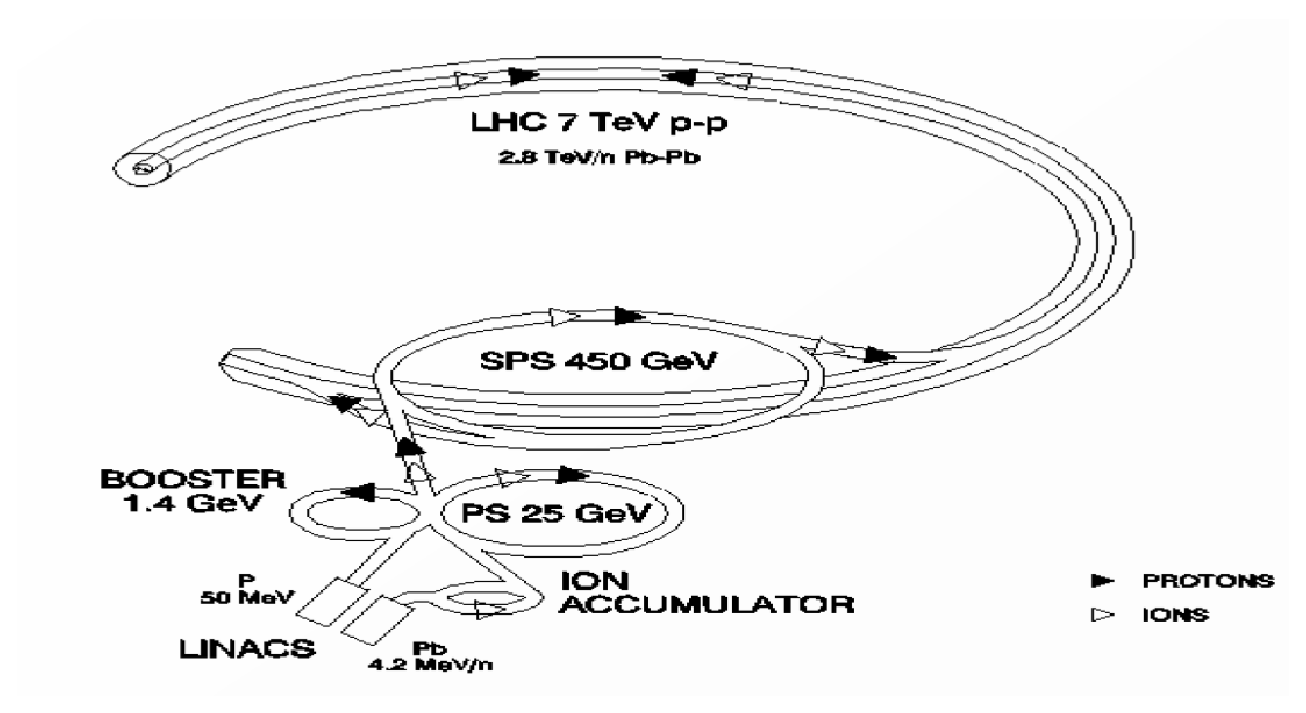
\includegraphics[width=0.6\linewidth,angle=0]{Detector/LHC_injection}
\end{center}
%\centerline{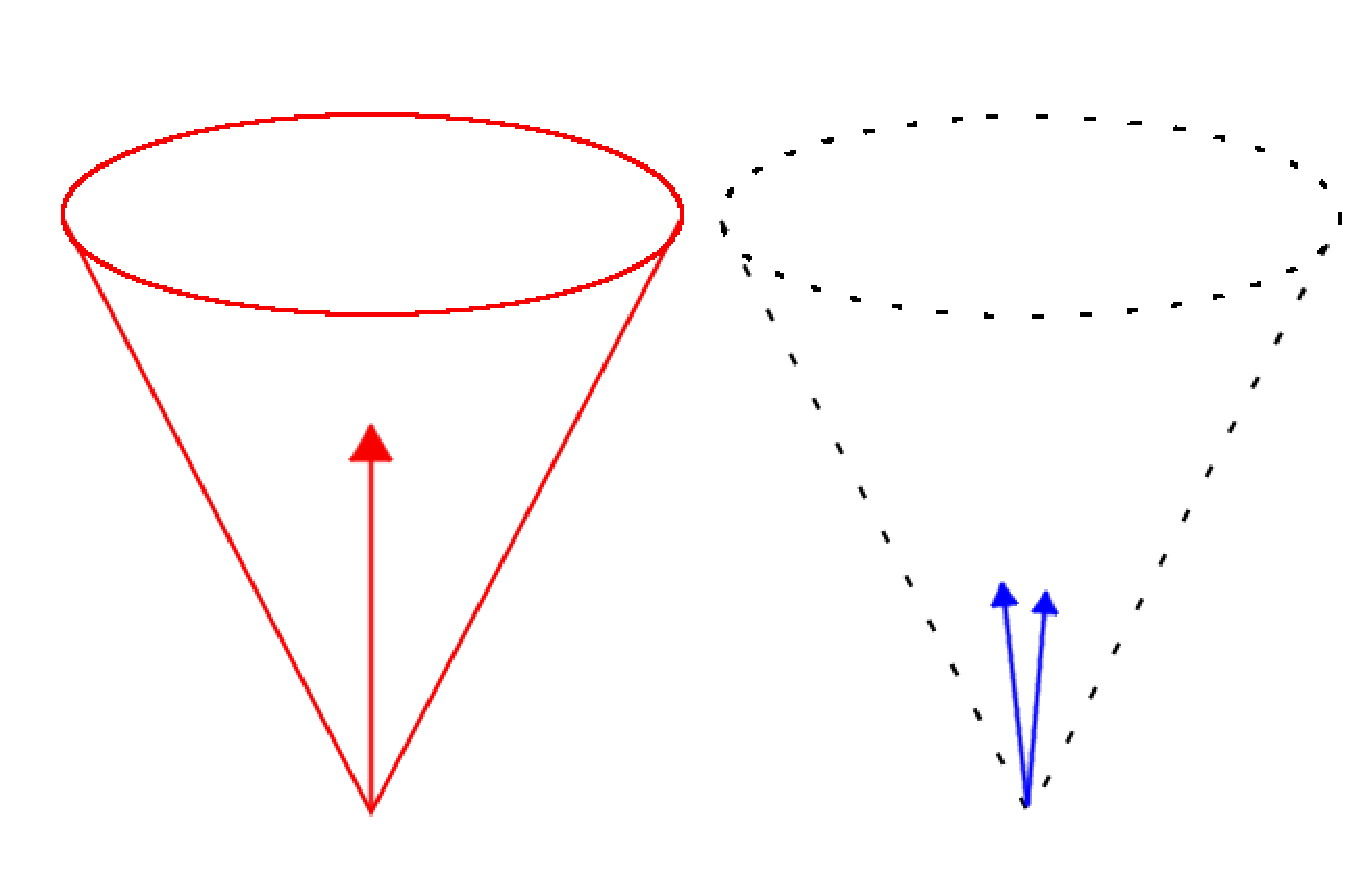
\epsfig{file=./figs/collinear.eps  , width=0.95\textwidth}}
\caption{Injection chain for protons and ions feeding the LHC. }
\label{LHC_inject}
\end{figure}

The injection chain for beam particles is shown in Figure~\ref{LHC_inject}. Hydrogen gas is used as a source of protons. Gas molecules are ionised in a duoplasmotron\cite{LHC_proton_source}, which emits protons at an energy of 90 keV. The protons are then accelerated to 750 KeV in a Radio Frequency Quadrupole (RFQ) before being accelerated to 50 MeV in a linear accelerator (LINAC2). A series of synchrotrons (the Proton Synchrotron Booster (PSB), Proton Synchrotron (PS), and Super Proton Synchrotron (SPS))  are then used to accelerate protons to energies of 1.4 GeV, 25 GeV and 450 GeV, respectively. After acceleration by the SPS, beams are injected into the LHC. Superconducting Radio-Frequency (RF) cavities are then used to accelerate the protons to their final energy.  Each LHC beam is designed to hold up to 2808 bunches\footnote{Currently only half of these bunches are being filled, such that bunch crossings are seperated by 50 ns.}, each containing $\sim 10^{11}$ protons, which are separated in time by 25 ns. 

%integrated/instantaneous relative to design
%
%expected to be operating at design parameters by 
%
%The proton beams are then injected into the LHC, 


\section{The ATLAS Detector}
The \atlas detector\cite{detector_paper} (shown in Figure~\ref{fig_ATLAS}) is a multi-purpose detector used to analyse collisions at the LHC. It is one of two multi-purpose detectors, the other being the Compact Muon Solenoid (CMS)\cite{CMSdetector}. \atlas consists of sophisticated particle tracking systems, a system of calorimeters, and a Muon Spectrometer, each of which will be discussed below. The Inner Detector (ID) and Muon Spectrometer (MS) will be discussed only briefly, as they play little role in the analyses discussed in this thesis. This chapter will focus on the calorimeters of \atlas, as these are used to reconstruct jets. Particular attention is paid to the forward calorimeters, as one of these was the subject of the beam test discussed in Chapter~\ref{chapTB}, and also because the forward calorimeters are responsible for the large kinematic coverage achieved in the inclusive jet and dijet cross-section measurements that are described in Chapter~\ref{INCJETCHAPTER}.
\begin{figure}[tb]
\begin{center}
\includegraphics[width=0.8\linewidth,angle=0]{Detector/ATLAS_overview}
\end{center}
%\centerline{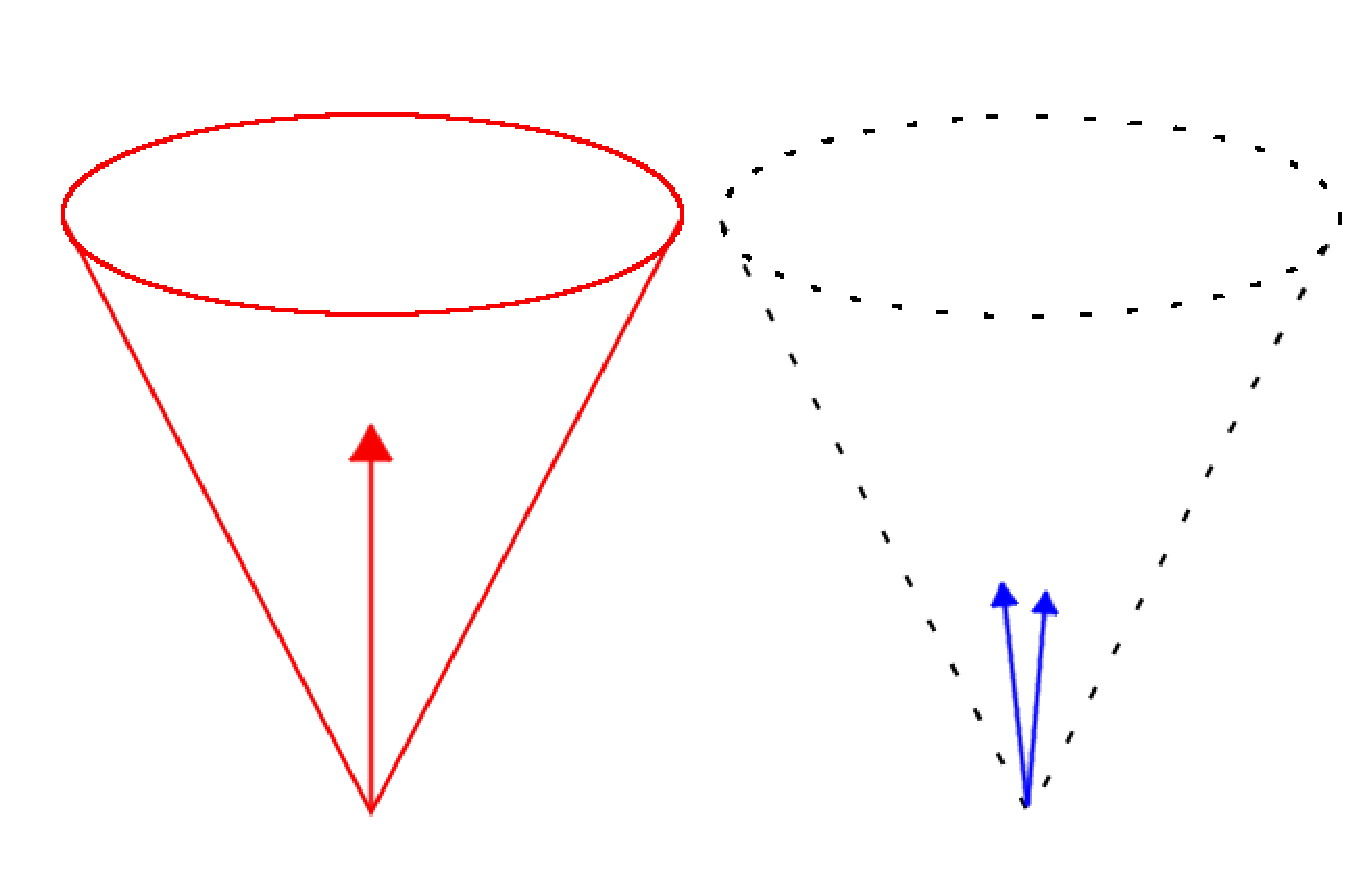
\epsfig{file=./figs/collinear.eps  , width=0.95\textwidth}}
\caption{Diagram of the ATLAS detector.}
\label{fig_ATLAS}
\end{figure}

\subsection{Coordinates}

\atlas uses a right-handed Cartesian coordinate system. The nominal interaction point at the centre of \atlas is defined to be the origin of this coordinate system, with the beams running along the $z$ axis. The positive $x$ axis points towards the centre of the LHC ring, while the positive $y$ axis is perpendicular to the other two, and points upwards. Parts of the detector are labelled according to which side of the interaction point they are located on. The ``A-side'' refers to objects located at positive values of $z$, while objects located at negative $z$ are said to be on the ``C-side''\cmt{which is especially nice during the summer}. \atlas is divided into a barrel and two end-cap sections. Each of these sections contains a cryostat, as (most of) the \atlas calorimetry is based on liquid argon technology.


The polar angle $\theta$ defines the angle from the beam axis, while the azimuthal angle $
\phi$ defines the angle around the beam axis. The direction $\theta = 0$ points along the positive $z$ axis, while $\phi = 0$ corresponds to the positive $x$ axis. The pseudorapidity, $\eta$, is defined using the polar angle $\theta$, such that 
\begin{equation}
\eta = - \log \left( \tan \left( \frac{\theta}{2} \right) \right).
\label{eqn_pseudorapidity}
\end{equation}
Pseudorapidity is an approximation to rapidity, $y$. The rapidity of an object with energy $E$ is given by
\begin{equation}
y = \frac{1}{2} \log \left(\frac{E+p_z}{E - p_z}\right),
\label{eqn_rapidity}
\end{equation}
where $p_z$ is the $z$ component of the objects momentum. The rapidity may be used to define a boost along the $z$ axis, such that in the boosted frame of reference the object's momentum will be perpendicular to the beam direction. In the limit where the mass of the object is negligible, pseudorapidity and rapidity are equivalent. Detector regions are typically described in terms of $\eta$, due to the one-to-one correspondence with $\theta$. Rapidity is often used when discussing kinematics, as differences in rapidity are invariant with respect to boosts in the direction of the beam.




 

%blah blah \atlas is blah blah



%\section{Coordinates}
%
%nominal interaction point defined as origin
%
%beam runs along z axis
%
%A side is positive z, C side negative
%
%positive x points towards centre of LHC ring
%
%positive y points up
%
%azimuthal angle, phi = 0 means in the x-z plane
%
%pseudorapidity defined as
%
%rapidity is ..., in the case of massive objects


%maybe?
\subsection{Inner Detector}
The Inner Detector (ID) is used to reconstruct the trajectories (tracks) of charged particles produced during proton-proton collisions. It is comprised of three systems: the pixel detector, the SemiConductor Tracker (SCT), and the Transition Radiation Tracker (TRT). These three components are contained within a cylindrical region of length 3.5m and radius 1.15m centred on the \atlas interaction point. The \atlas solenoid is a superconducting magnet located just outside of the ID, in the barrel cryostat, and generates a 2T magnetic field oriented along the $z$ axis in the region occupied by the ID. The applied field gives rise to curvature in the trajectories of charged particles, such that measurements of particle trajectories can be used to determine the transverse momentum (\pt) of those particles. The ID is also used for vertex reconstruction at \atlas. The primary vertex is associated with the location of the hard inelastic collision, while other soft collisions may produce additional secondary vertices. The accuracy with which a given vertex position may be reconstructed is dependent on the number of tracks associated with the vertex and the \pt~of those tracks. In cases where there are at least 70 tracks emerging from the primary vertex and the quadratic sum of track \pt~ values\cmt{when added in quadrature} exceeds 8 GeV, the primary vertex can be determined with an accuracy of $\sim$30 $\mu$m in the transverse plane and $\sim$50 $\mu$m in the longitudinal direction\cite{vertex_ref}.

%primary vertex -> hard inelastic collision location
%accuracy dependant on tracks.
%resolution

%which can then be used to obtain measurements the transverse momentum (\pt) of the track.

The inner detector consists of a barrel section (shown in Figure ~\ref{fig_ID_barrel}) and two end-cap sections (Figure \ref{fig_ID_EC}). 
\begin{figure}[p]
\begin{center}
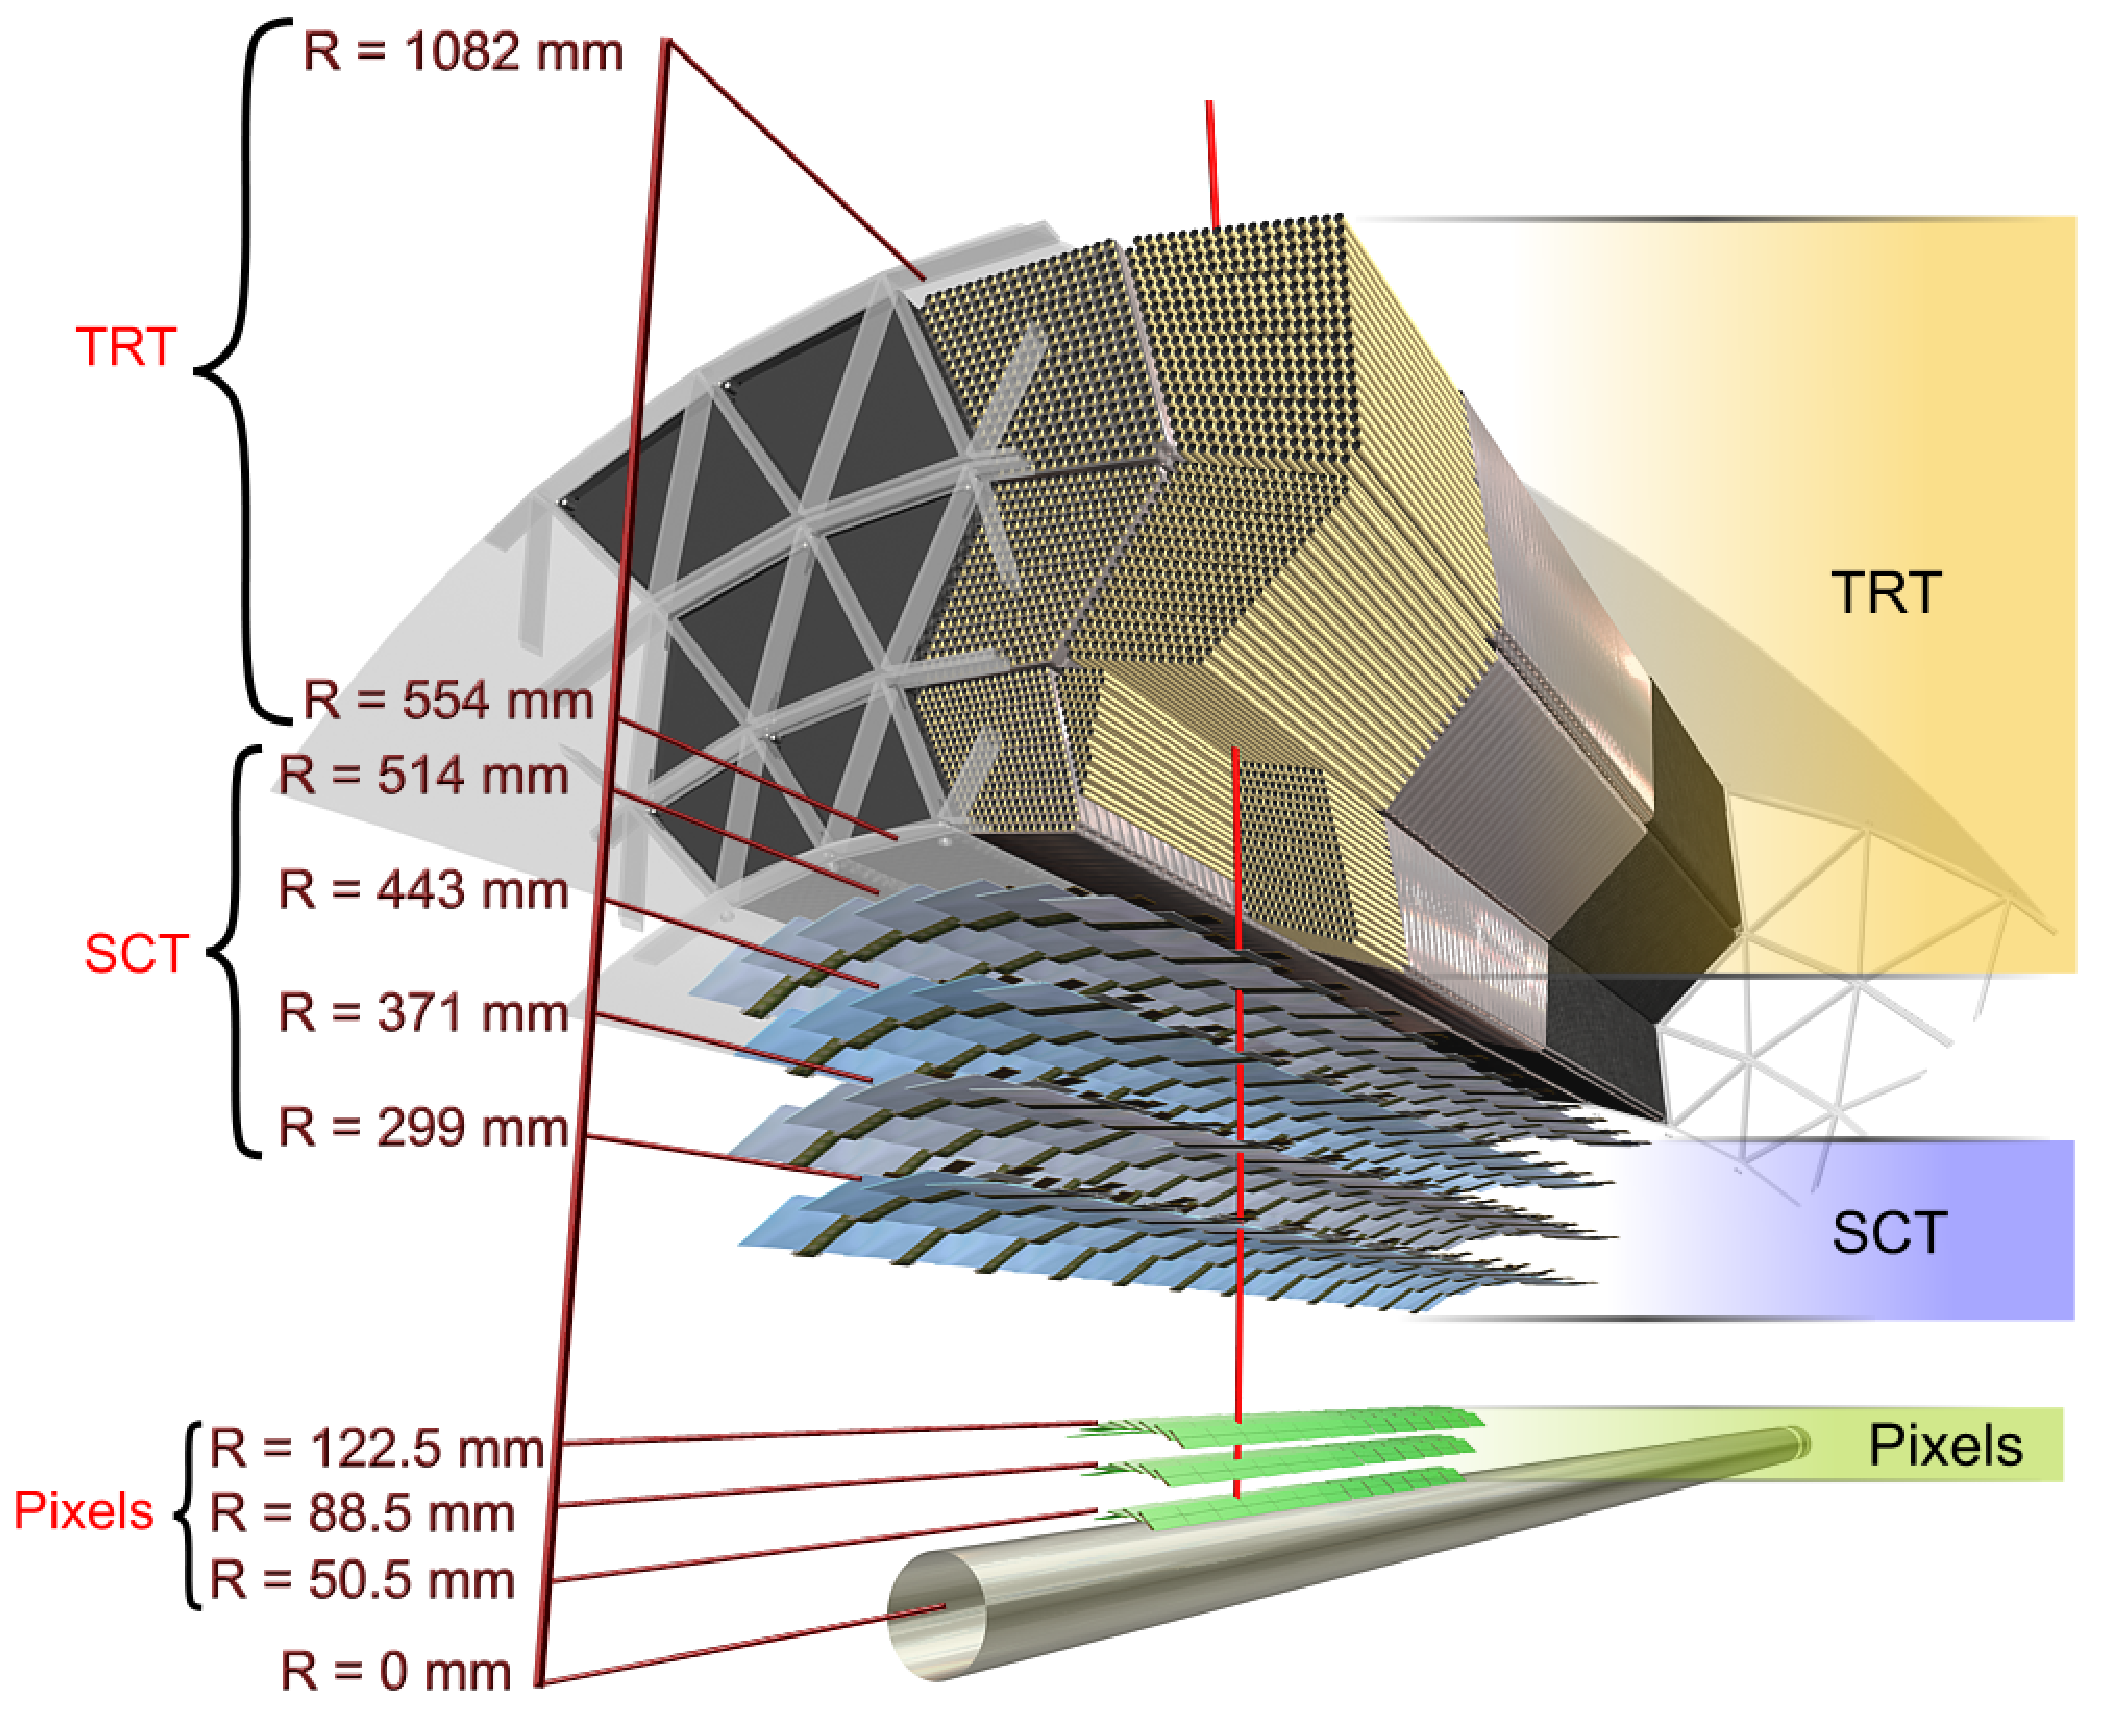
\includegraphics[width=0.8\linewidth,angle=0]{Detector/ID_barrel}
\end{center}
%\centerline{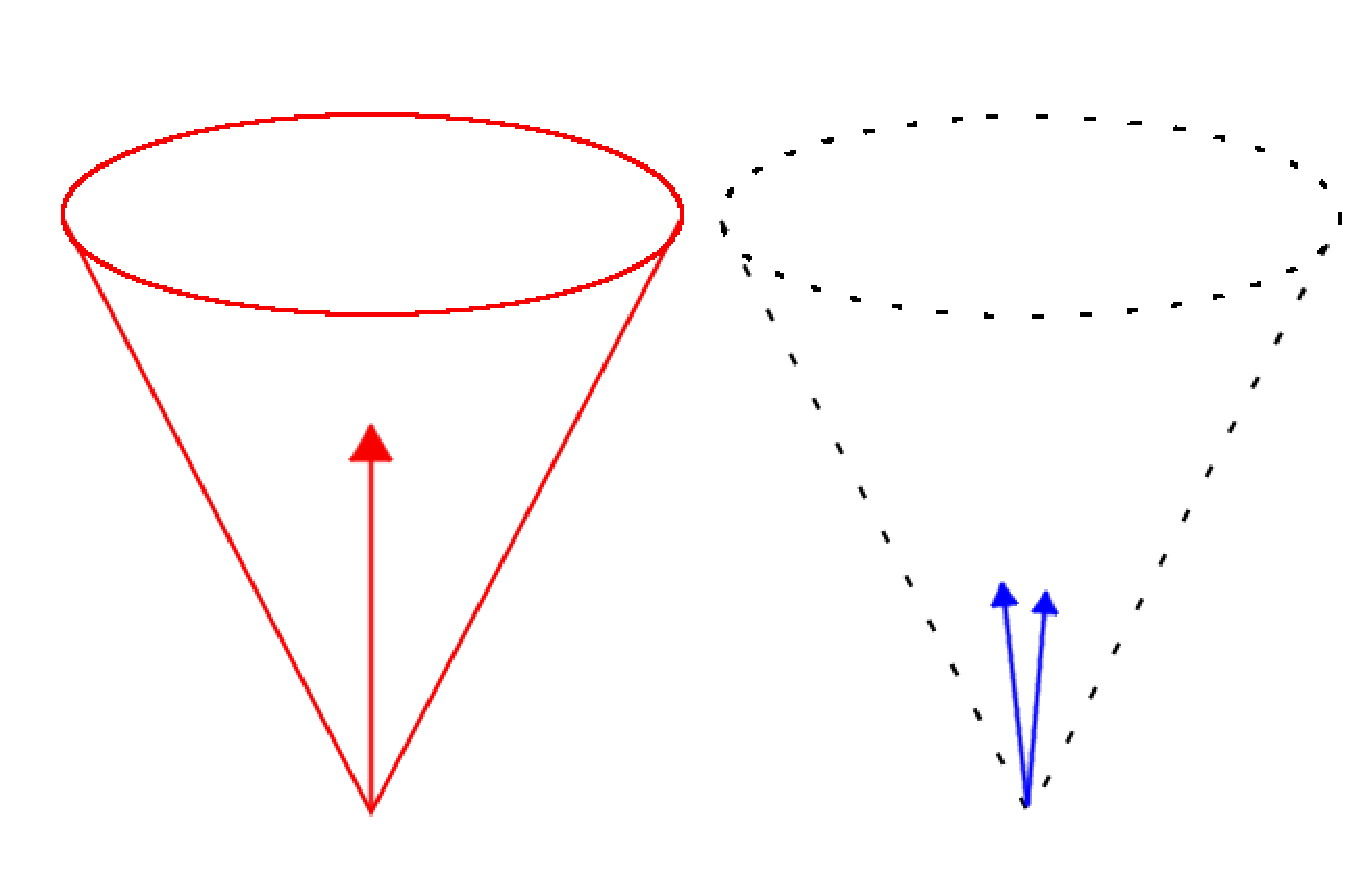
\epsfig{file=./figs/collinear.eps  , width=0.95\textwidth}}
\caption{Diagram of the barrel section of the inner detector.}
\label{fig_ID_barrel}
\end{figure}

\begin{figure}[p]
\begin{center}
\includegraphics[width=0.6\linewidth,angle=0]{Detector/ID_endcap}
\end{center}
%\centerline{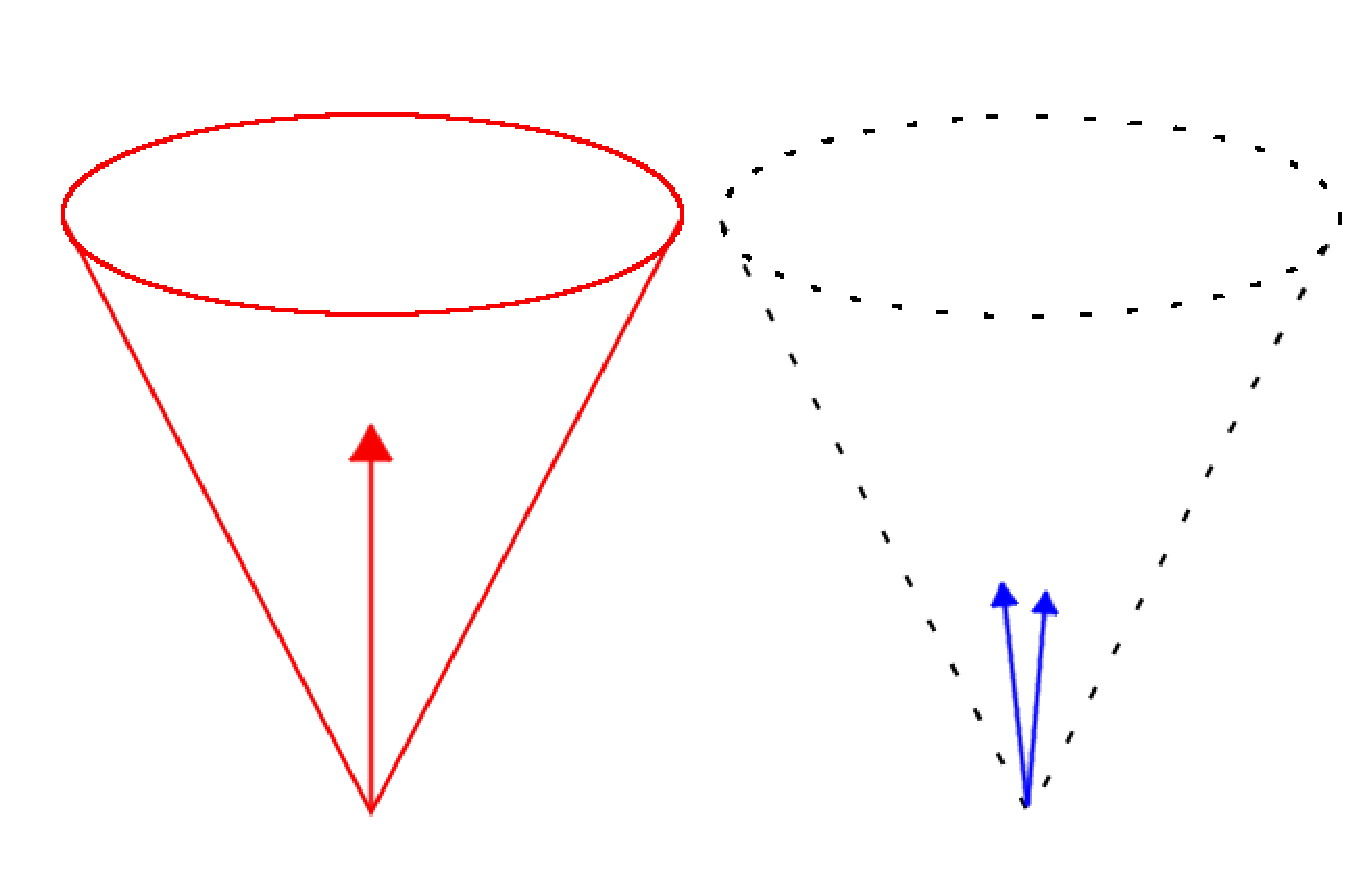
\epsfig{file=./figs/collinear.eps  , width=0.95\textwidth}}
\caption[Diagram of the inner detector]{Diagram of the inner detector, showing the elements traversed by particles at pseudorapidities of 1.4 and 2.2.}
\label{fig_ID_EC}
\end{figure}
%Each component of the inner detector is comprised of one barrel and two end-cap sections, as shown in figure~\ref{}

The pixel detector uses sensors formed from 250$\mu$m thick wafers of silicon. The barrel section consists of three cylindrical layers, and three disc-like layers are used to form each end-cap. All together there are $\sim 8 \times 10^7$ pixel channels, which are designed to provide a hit resolution of 10 $\mu$m in the $R-\phi$ plane and 115 $\mu$m in the $z$ direction in the barrel section. \cmt{something about radiation hardness}

The SCT is located beyond the pixel detector, and consists of 4 cylindrical layers in the barrel section and 9 disc layers in each end-cap. Each SCT module has semiconducting microstrip sensors mounted on both sides that are oriented at an angle of 40 mrad to each other. As a single microstrip sensor only provides a position measurement in one dimension, orienting two at a slight angle allows the position of the hit to be measured in two dimensions, by correlating hits in the two sensors. The SCT is designed to have a resolution of 17 $\mu$m in the $R-\phi$ plane and 580 $\mu$m in $z$.

The TRT is the outermost section of the inner detector, and is formed from straw-shaped drift tubes. The barrel section contains $\sim$52,500 tubes, while $\sim$123,000 tubes are contained in each end-cap section. Straws are made from layers of polyimide, aluminium, polyurethane and graphite-polyimide. Each straw is 4mm in diameter, with a gold-plated tungsten wire (of diameter 31$\mu$m) located in the centre of the tube that serves as an anode. The gas in the tubes is 70\% Xe, 27\% $\mathrm{CO}_2$ and 3\% $\mathrm{O}_2$. Charged particles entering the tube ionise the gas, with the resulting electrons drifting towards the anode in the centre. Measurement of the electron drift time allows the distance of the particle track from the wire to be determined with a resolution of 130$\mu$m. 
The straw tubes are housed within a volume filled with $\mathrm{CO}_2$ and a matrix of polypropylene fibres (in the barrel section) or foils (in the end-caps). Electrons moving between the $\mathrm{CO}_2$/polypropylene interfaces emit transition radiation. This radiation (and the original electron) will then ionise the gas inside the tubes, inducing a signal on the tube anodes. Xenon is used because it efficiently absorbs the transition radiation photons, emitting photoelectrons in the process. Charged pions produce less transition radiation than electrons, and thus generate smaller signals. This difference in signal size allows the TRT to perform particle identification, discriminating electrons from charged pions.

%\red{Inner detector can also determine the vertex of the collisions and shit.}
%provides resolution (distance from wire) of 130 $\mu$m 

%27% CO2, 3%O2 70% Xe


%also used to reconstruct vertices
%
%The pixel detector is innermost, consists of X layers containing Y channels. Resolution of X $\mu$m.
%Consists of layers of semiconducting silicon wafers.
%
%
%n type silicon wafers, oxygenated in order to improve radiation tolerance. Pixel is right next to the IP, so it needs to be radiation hard, to last 10 years or so.
%
%
%
%SCT lies beyond the pixel, covering (dimensions in xyz / eta phi). Consists of 4 cylindrical layers in the barrel section and 9 disks in each side of the end-cap.
%sort out what exactly the stereo deal is.
%
%inner detector covers up to 2.5, tracks charged particles
%
%
%pixel, SCT, TRT
%pic
%
%pixel has X number of strips, dimensions, channels, resolution
%
%SCT, semiconductor tracker (?)
%
%TRT transition radiation tracker - how does this work (exactly)?
%
%
%materials/gasses




%I know nothing about the inner detector
%
%good fig on page 56 of detector paper
%
%ID coverage up to |eta|< 2.5
%electron id for |eta < 2.0, 0.5 GeV < E < 150 GeV
%
%+- 3512mm, r = 1150mm
%solenoid field 2T
%
%pixel, SCT, TRT (dimensions on p55 of Detector paper)
%innermost pixel replaced every three years of running at design luminosity
%3 layers of pixel, 4 layers of SCT
%
%
%
%pixel
%250um thick, ``oxygenated n-type wafers"



%\clearpage
\subsection{Muon Spectrometer}

The Muon Spectrometer is the outermost system of the \atlas detector, and is illustrated in Figure~\ref{fig_Muon_bits}. It is designed to measure muons in the region $|\eta| < 2.7$ with a momentum resolution of $\sim 10\%$ at 1 TeV. However, during 2010 running muons were measured with a resolution of $\sim 5\%$ at 100 GeV in the barrel region\cite{muon_bs}: when the fit to this data is extrapolated, it corresponds to a resolution of $\sim$25\% at 1 TeV. The Muon Spectrometer is also capable of triggering on muons in the region $|\eta| <2.4$. The Muon Spectrometer is comprised of four types of detectors: Monitored Drift Tubes (MDTs), Cathode Strip Chambers (CSCs), Resistive Plate Chambers (RPCs) and Thin Gap Chambers (TGCs). The MDTs and CSCs are referred to as ``precision chambers'' and are used to measure the kinematics of muons, while the TGCs and RPCs are used for triggering and measuring the $\phi$ coordinates of muon tracks.

\begin{figure}[tb]
\begin{center}
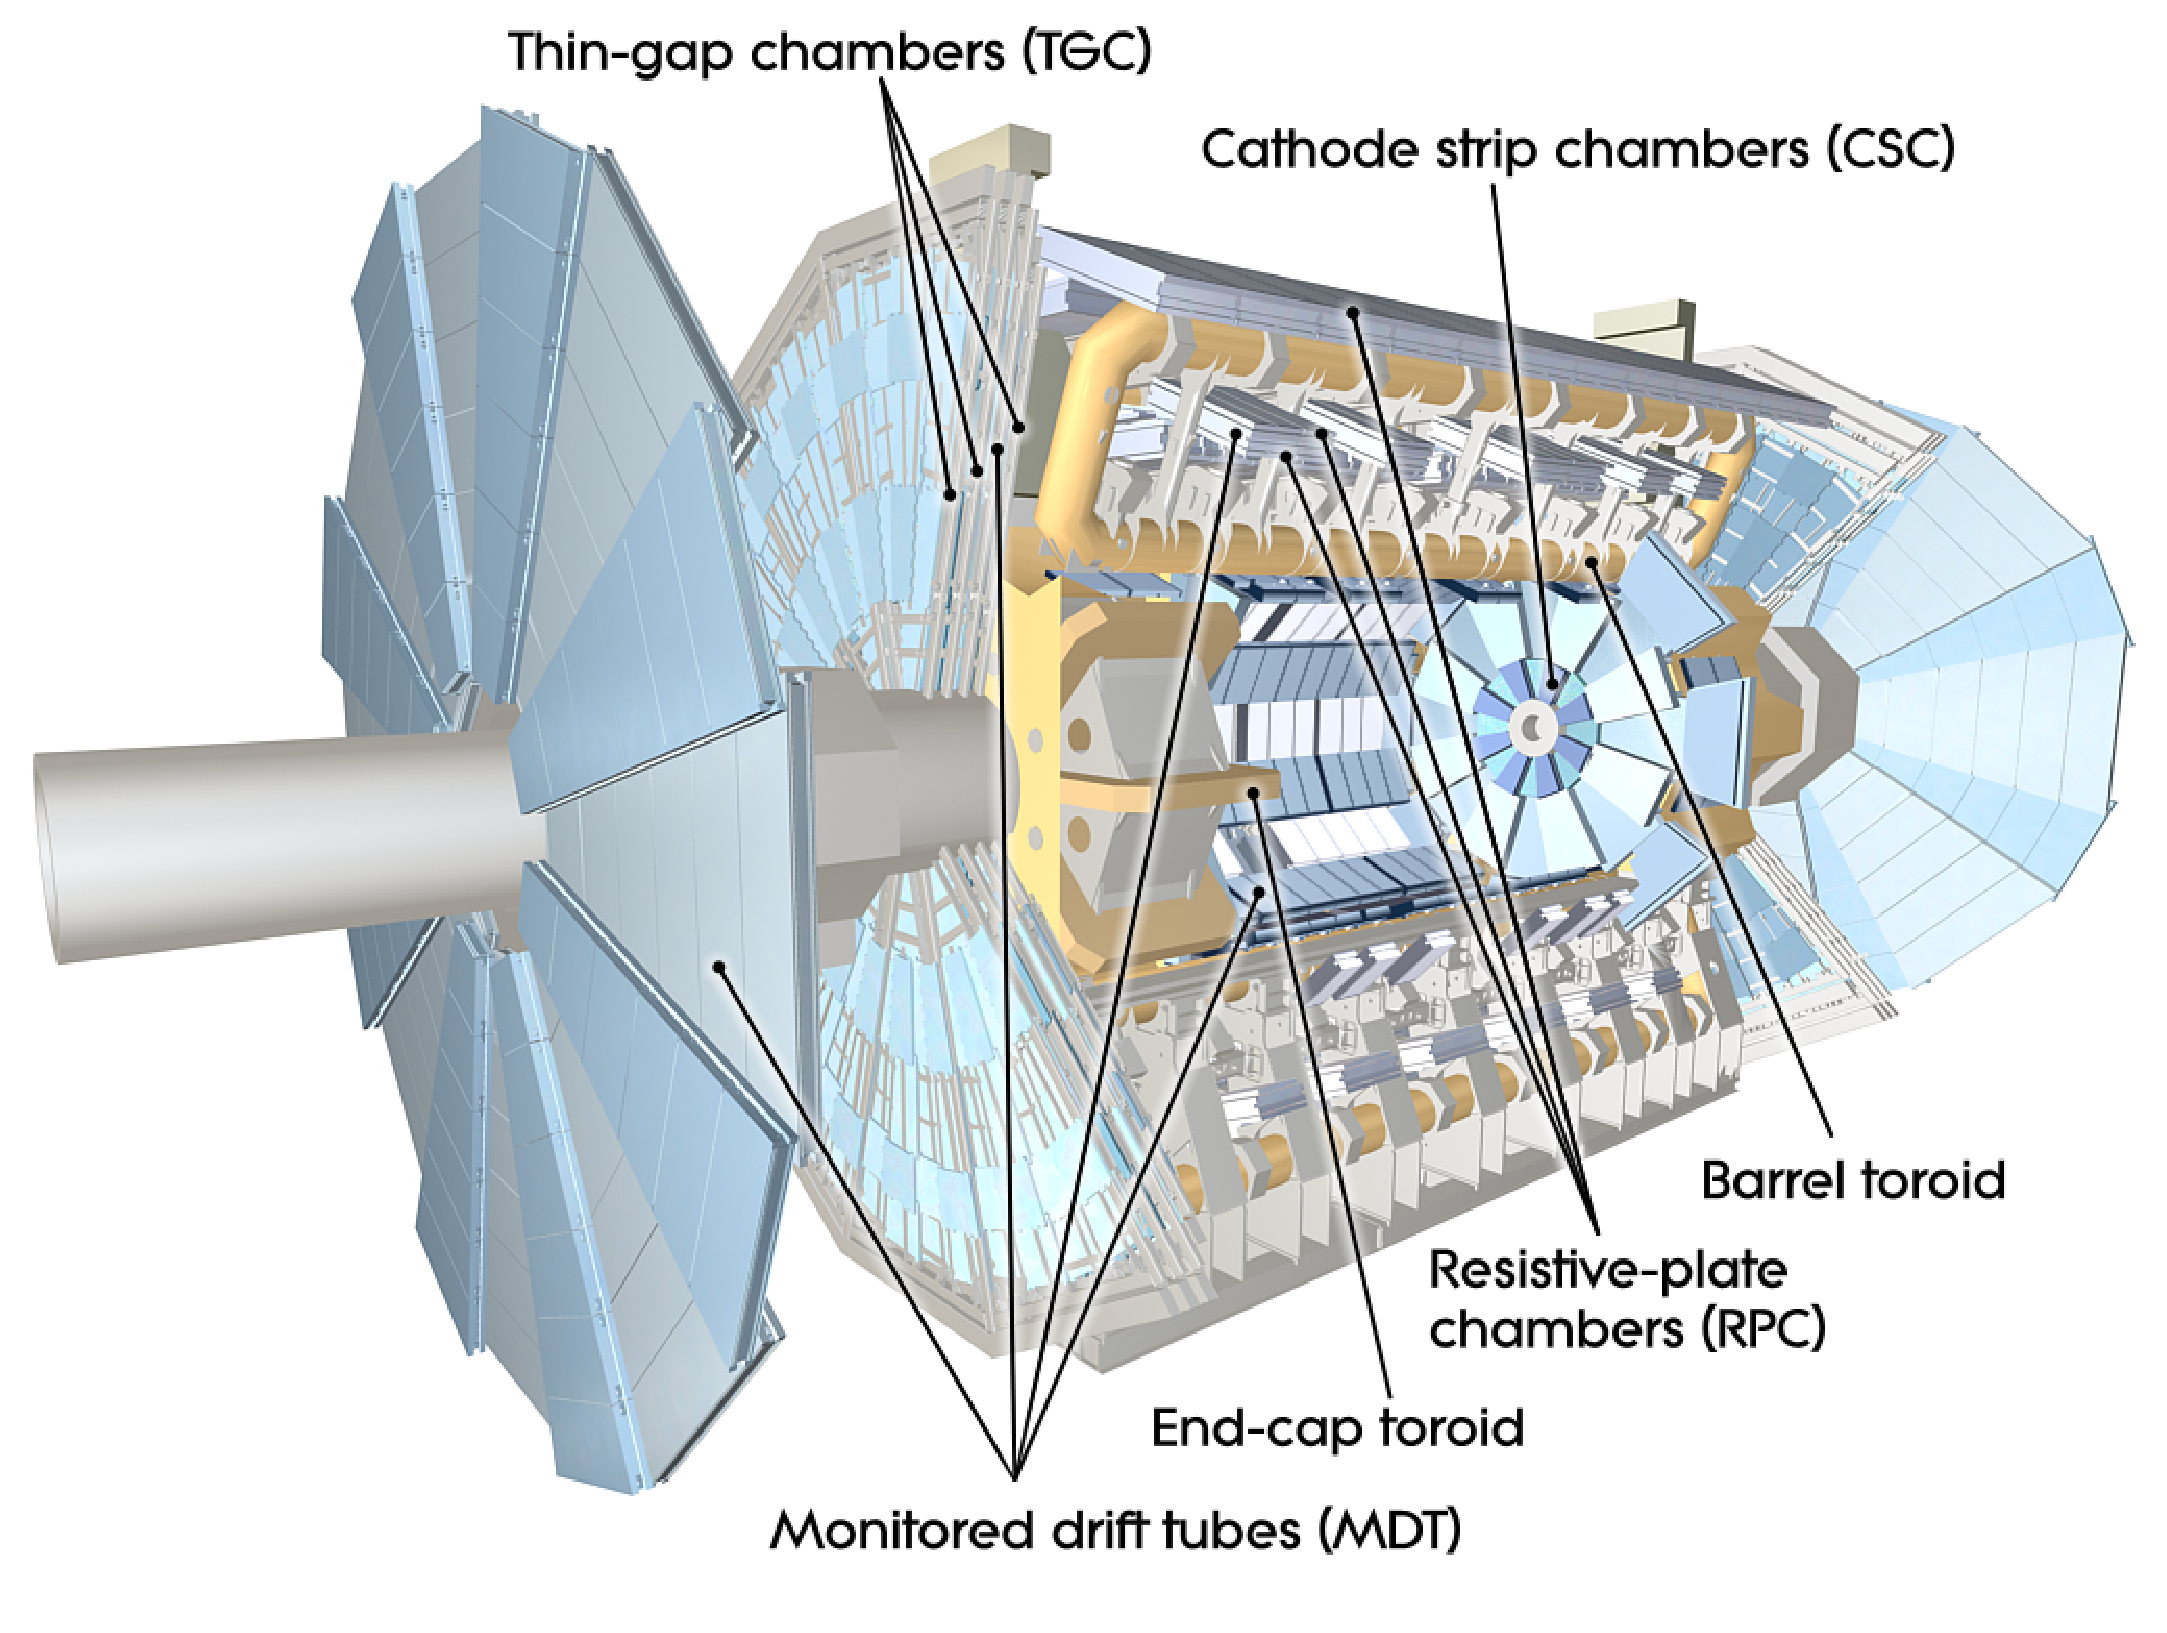
\includegraphics[width=0.8\linewidth,angle=0]{Detector/Muon_bits}
\end{center}
%\centerline{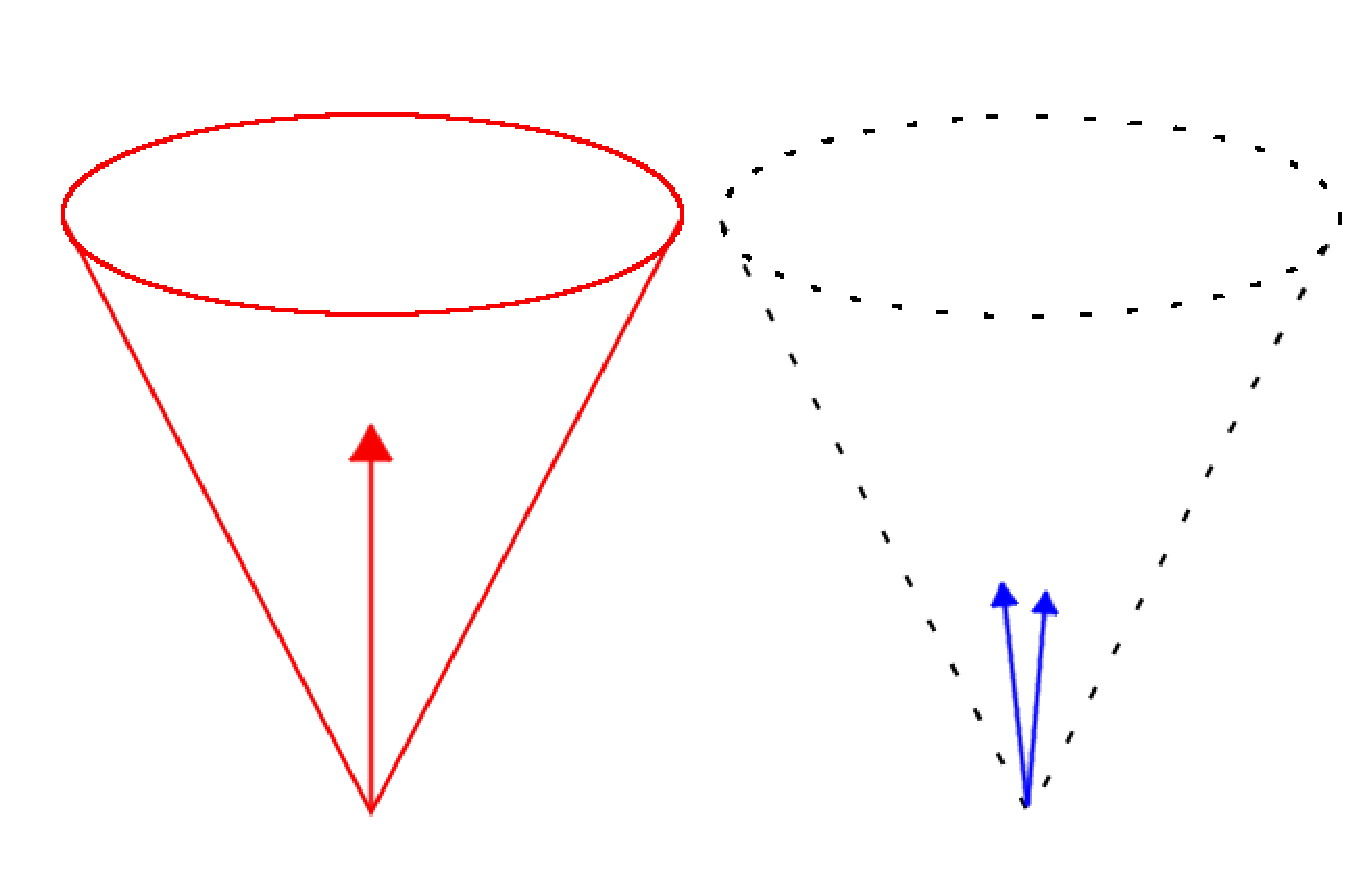
\epsfig{file=./figs/collinear.eps  , width=0.95\textwidth}}
\caption[Components of the Muoin Spectrometer.]{The different components of the Muon Spectrometer. The MDT and CSC components are used for measuring muon momenta, while the RPCs and TGCs are used primarily for triggering.}
\label{fig_Muon_bits}
\end{figure}


Superconducting toroidal magnets (the barrel toroid and two end-cap toroids) are located beyond the calorimeters. 
These produce a toroidal field (i.e. one in which the field lines run in the azimuthal direction), which causes charged particles to bend in the $R-z$ plane. In order to measure track momenta with high resolution, the relative alignment of the MDT and CSC chambers must be well known. A high precision optical system is used to monitor the positions and mechanical deformations of the measurement chambers, which must be known to within 30 $\mu$m in order to achieve the desired momentum resolution.

MDTs are comprised of cylindrical drift tubes of diameter 29.97mm, with a central anode wire of diameter 50$\mu$m. A mixture of Argon (93\%) and $\mathrm{CO}_2$ (7\%) is used to fill the tubes. Each drift tube is capable of measuring the distance of a muon track from the anode wire with a resolution of 80$\mu$m. The tubes are grouped together to form chambers. There are three (roughly) cylindrical layers of chambers in the barrel (at radii of 5 m, 7.5 m and 10 m), and four layers in each end-cap.

%tubes are grouped together into chambers. Three layers of chambers in the barrel section, and two layers in each end-cap


MDTs are used in all four layers of the end-cap sections. However, in the forward region ($|\eta | > 2.0$) of the innermost layer (located at $z \approx 7.4$ m) CSCs are used instead, as the MDTs are unable to operate in the high levels of radiation present in this region. The CSCs are multi-wire proportional chambers (MWPCs), filled with a mixture of Argon (80\%) and $\mathrm{CO}_2$ (20\%), and are capable of measuring hit positions to within 60 $\mu$m in the bending plane.

For triggering purposes, RPCs are used in the barrel region ($|\eta| < 1.05$) while TGCs (which are a form of MWPC) are used in the end-cap region ($1.05 > |\eta| > 2.4$). The intrinsic response time of these detectors is on the order of a few nanoseconds, enabling them to reliably identify the bunch crossing in which any detected muons were produced.
\subsection{Calorimetry}

\subsubsection{Sampling Calorimeters}

All of the calorimeters used at \atlas are sampling calorimeters, which consist of active regions and passive (absorbing) regions. The active layers are sensitive: energy deposited in these regions produces a signal which is then read out. The passive regions are made from a denser absorbing material, which is used to regulate the shower size. Sampling calorimeters are less expensive to produce than homogenous calorimeters\cmt{, and tend to occupy less space: If a homogenous calorimeter can completely contain a shower in a given volume, then a sampling calorimeter made using the same active material will be able to contain the shower in a smaller volume}.

 Sampling calorimeters may be characterised by their sampling fraction, which is defined as the energy deposited in the active regions by a minimum ionising particle (MIP) divided by the total energy deposited in the active and passive regions by the MIP~\cite{wigmans2000calorimetry}.
%
%calorimeter designs consist of active layers and a passive layers of absorbing material. Absorbing material dense, there to reduce shower size, active layers sensitive: energy deposited in these regions produces a signal that is read out.

Most of the \atlas calorimeters are based on liquid argon (LAr) technology, i.e. LAr is used to form the active regions of the calorimeter. Charged particles passing through these active regions ionise the liquid argon. The liberated electrons then drift in an applied electric field, resulting in an induced current pulse. This current is then used as a signal.

The \atlas Tile calorimeter uses tiles of scintillating polystyrene as the active material. These are positioned between layers of steel (the passive material). Charged particles passing through these tiles excite the scintillating material, which then produces photons. This scintillation light is then wavelength shifted in order to prevent it from being reabsorbed by the scintillating material, and then carried by optical fibres to photomultiplier tubes (PMTs), which absorb the light and produce an electrical signal.

%Sampling fraction. defined as the visible (signal-producing) energy deposited in active region divided by the total energy deposited in the calorimeter.
%Sampling calorimeters are characterised by their sampling fraction, which is defined as the total energy  


\subsubsection{Electromagnetic Shower Development}

Photons and electrons interact with the calorimeter via electromagnetic (EM) processes. The dominant processes by which electrons (or positrons) lose energy while traversing the material of the calorimeter are ionisation and Bremsstrahlung. At high energies Bremsstrahlung dominates, while at lower energies ionisation is the dominant process. The critical energy, $\epsilon_c$, is defined as the value of an electron's energy at which the rate of energy loss via ionisation is equal to the rate of energy loss from Bremsstrahlung. This value  is material dependent, but an approximation for solids and liquids is given by\cite{wigmans2000calorimetry}

\begin{equation}
\epsilon_c = \frac{610 \mathrm{MeV}}{Z + 1.24}
\end{equation}
where $Z$ is the atomic number of the element being traversed.

The longitudinal extent of an EM shower may be expressed in terms of the radiation length, which is the distance over which an electron loses $\sim63\%$  ($1- e^{-1}$) of its energy via Bremsstrahlung. The radiation length of a material may be approximated by\cite{ReviewPP98}
\begin{equation}
X_0 = \frac{716.4 \,A }{Z(Z+1) \log(287/\sqrt{Z})} \quad \mathrm{g cm}^{-2},
\end{equation}
where $Z$ is the atomic number of the element. Note that the expression has units of $\mathrm{g~cm}^{-2}$, and so should be divided by the density of the material in order to obtain a value with dimensions of length. In cases where the material is comprised of multiple elements, then the radiation length of the compound is given by
\begin{equation}
\frac{1}{X_0} = \sum_j \frac{w_j}{X_{0,j}},
\end{equation}
where the $X_{0,j}$ and $w_j$ are, respectively, the radiation length and fraction (by mass) of the $j$-th element.

A similar quantity exists to describe the lateral extent of an EM shower. The \moliere radius, $\rho_M$, is given by 
\begin{equation}
\rho_M = X_0 \frac{21.2 \mathrm{MeV}}{\epsilon_c}.
\end{equation}
Unlike the radiation length, the \moliere radius doesn't have a strict physical meaning, although roughly $80-90\%$ of an EM shower's energy is generally deposited within a cylinder of radius $\rho_M$~\cite{wigmans2000calorimetry}.


The dominant processes for photons are pair production, Compton scattering and the photoelectric effect. At higher energies ( $  \gtrsim 10$ MeV) pair production is the most likely, though as the photon's energy decreases Compton scattering becomes more prevalent, while the photoelectric effect dominates at the lowest energies ( $\lesssim 1$ MeV). The average distance that a high energy photon travels before undergoing pair production is 9/7 $X_0$.

Typically, EM showers consist of successive Bremsstrahlung and pair production interactions. An initial electron will radiate, producing a photon. The photon will then undergo pair production, yielding an electron-positron pair in addition to the original electron. This process then repeats, with electrons and positrons radiating photons that then convert into additional electron-positron pairs. This continues until the electron/positron energies fall below the critical energy, at which point they are more likely to lose energy via ionisation than through further radiation. The energy of the initial electron is thus divided between all the electrons and photons produced during the shower, with the electrons then depositing their energy in the calorimeter via ionisation. Ionisation in the active layers of a calorimeter is used to generate a signal: in the LAr calorimeters the ionisation induces a current in the electrode, which is used as a signal, while in the Tile it produces photons via scintillation, which are then guided to a photomultiplier tube and used to produce an electrical signal.
%
% 
% in which the the electric field of the passing electron causes another electron to be ejected from an atom of the material,and Bremsstrahlung radiation. Brems
%
%Electrons passing through a calorimeter will lose energy via Bremsstrahlung radiation or by ionising the calorimeter material. 
%explain these
%
%EM showers characterised by radiation length. For a given material ..
%
%
%radiation length is defined as the average length an electron will travel before losing $63\% (1-e^-1) $of its energy via Bremsstrahlung radiation. an approximation for this is given by 


\subsubsection{Hadronic Shower Development}
\label{detector_had_showers}
While EM showers tend to be dominated by only a few processes, there are many more processes that may take place in a hadronic shower, making them more complex. 

The longitudinal development of hadronic showers is characterised by the nuclear interaction length, $\lambda_\mathrm{int}$, which describes the average distance that a hadron will travel in a material before interacting with a nucleus. In general, $\lambda_\mathrm{int}$ scales as $A^{1/3}$, where $A$ is the mass number of the element being traversed.

Hadronic showers have an EM component and a non-EM component. Of the $\pi$ mesons produced in hadronic interactions, roughly 1/3 are $\pi^0$ mesons. The decay $\pi^0 \rightarrow \gamma \gamma$ occurs very quickly (at rest, the $\pi^0$ has a lifetime of $8.5 \times 10^{-17}$s), with a branching fraction of 99\%~\cite{reviewPP2012}. Thus, almost all the $\pi^0$'s produced in hadronic showers go on to induce EM showers. At each interaction, some of the energy carried by the non-EM component is redirected into the EM component. As the energy of the initial hadron increases, the number of interactions (and thus the fraction of energy carried by the EM component) increases also. The energy carried by the EM component thus scales non-linearly with the energy of the initial hadron. 

A feature of the non-EM component of hadronic showers is that some of the energy deposited in the active layers is invisible to the calorimeter. For instance, when a showering hadron interacts with a nucleus and frees a number of nucleons, the binding energy required to release those nucleons is essentially lost: it is invisible to the calorimeter. Neutrons are produced in large quantities during nuclear interactions, and while these may undergo further nuclear interactions they will not ionise the active region of the calorimeter, and so in that sense are invisible. Furthermore, hadronic interactions with nuclei may produce particles that decay to muons and/or neutrinos. Muons (unlike electrons) deposit a minimal amount of energy via ionisation before leaving the calorimeter, while neutrinos (almost always) leave the calorimeter without interacting at all.

A calorimeter will have a lower response to a hadronic shower than it would to an EM shower of the same initial energy, unless it somehow corrects for this invisible energy. This correction is referred to as compensation.
%  Compensation may be achieved by boosting the response to the non_em component of the shower, diminishing the EM response, or both. 
 The most effective way to achieve compensation is by increasing the calorimeter's response to the non-EM shower component. This response may be boosted if the active material contains hydrogen (as is the case with scintillating materials). In this case, the neutrons produced in nuclear interactions can scatter off hydrogen nuclei. The active material is then sensitive to the recoiling proton~\cite{wigmans2008calorimetry}. Alternatively, using fissile material as an absorbing material can boost the non-EM response. Energy released in fission reactions can compensate for invisible energy losses. The ZEUS\cite{zeus} calorimeter is based on uranium/scintillator technology, and is an example of a compensating calorimeter.\cmt{However, most of the energy released in fission carried by neutrons, so still need H in the active material.}
 
 
% nuclear interaction length, lambda_int, average distance hadrons travel before having a nuclear interaction. scales as A^1/3 (mass number)
  
The \atlas calorimeters are all non-compensating, and thus the response of the calorimeters to hadrons is lower than for electrons of the same energy. Software-based methods are used during offline reconstruction to correct for this effect, as described in sections~\ref{section_TB_hadron_results} and~\ref{section_JES}

\subsubsection{Calorimeter Energy Resolution}

%fluctuations. certain things can cause variations in the measured energy. 
The performance of a sampling calorimeter may be characterised in terms of its resolution, $\sigma/\bar{E}$, where $\bar{E}$ is the mean reconstructed energy and $\sigma$ is the RMS of the calorimeter response. The resolution is typically parameterised by a function of the form
\begin{equation}
\frac{\sigma}{\bar{E}} = \frac{A}{\sqrt{\bar{E}}} \oplus B \oplus \frac{C}{\bar{E}},
\label{eqn_resolution_general}
\end{equation}
where $A$, $B$, and $C$ are called the stochastic, constant, and noise terms, respectively, and $\oplus$ denotes addition in quadrature.

The stochastic term arises from variations in the sampled energy, for example, an incident particle may shower in a way that deposits a large amount of energy in the active regions of the calorimeter, or in a way that deposits less energy in these regions. These sampling fluctuations are governed by Poisson statistics, and thus give rise to a term proportional to $\bar{E}^{-1/2}$ in the resolution\cite{fabiola_calorimetry}.

The constant term arises from effects that are independent of energy deposited in the detector, such as non-uniformities in the calorimeter response. These non-uniformities may be caused by uninstrumented material in front of the calorimeter, irregularities in the calorimeter structure, or damage caused by radiation or aging, or a calorimeter design in which the response is dependent on the impact point of the incident particle. This impact point dependence forms the dominant contribution to the constant term for the forward calorimeters of \atlas, which is discussed further in section~\ref{TB_results_electrons}.

The noise term is associated with electronic noise in the readout chain. For the liquid argon calorimeters used at \atlas, the majority of this noise is introduced in the preamplifiers which are located on the front end boards. The noise contribution is independent of the signal being read out of the channel, and so the noise term in the resolution scales as $\bar{E}^{-1}$.


%Sampling calorimeter performance characterised by its resolution, sigma/e, where E is the mean reconstructed energy and sigma is the rms of the calorimeter response.
%
%calorimeter resolution may typically be parameterised by a function of the form
%
%
%A, B and C are the stochastic, constant, and noise terms, respectively, and $\oplus$ denotes that the terms should be added in quadrature.
%
%stochastic term arises from variations in the sampled energy, that is, incident particle may shower in a way that deposits a large amount of energy in the active regions of the calorimeter, or in a way that deposits less energy in these regions. these fluctuations are governed by Poisson statistics, and thus give rise to a term proportional to 1/sqrt E in the resolution.
%
%noise term - electronic noise in the readout chain. For the liquid argon calorimeters discussed below, the majority of this noise is introduced in the preamplifiers. noise independent of the energy  being read out from a given channel, and so contribution to the resolution proportional to 1/E
%
%constant term - energy independent things, like detector nonuniformities, etc. 
%
%
%Sampling calorimeters typically have 
%X0 =
%
%ec?

%length scale that characterises longitudinal development of EM showers.
%radiation length describes the mean distance that an electron travels before 
%
%Also, there is the Moliere radius
%
%describes the lateral development.
%
%
%
%
%Fucking Wigmans motherfucker
%
%or Em shower development
%
%hadronic shower development
%
%sampling calorimeters
%
%
%
%sampling calorimeters
%sampling fraction
%
%Em showers
%brems, pair production
%radiation length, Moliere radius
%
%hadronic showers
%invisible energy
%compensation
%(E dependence of EM component)
%
%
%hadronic showers
%
%hadronic showers deposit less visible energy in calorimeter than EM showers

\subsection{The ATLAS Calorimeters}



%The precision electromagnetic calorimeters are lead-liquid0
\atlas contains five distinct calorimeters, shown in Figure~\ref{fig_calorimeters}. The Electromagnetic Barrel (EMB) Calorimeter is located in the central ``barrel'' section of \atlas, while the Electromagnetic End-cap Calorimeter (EMEC), Hadronic End-cap Calorimeter (HEC) and Forward Calorimeters (FCal) are located within the end-caps at either end. The Tile calorimeter consists of barrel section, and two extended barrel sections that surround the end-cap cryostats.
\begin{figure}[tb]
\begin{center}
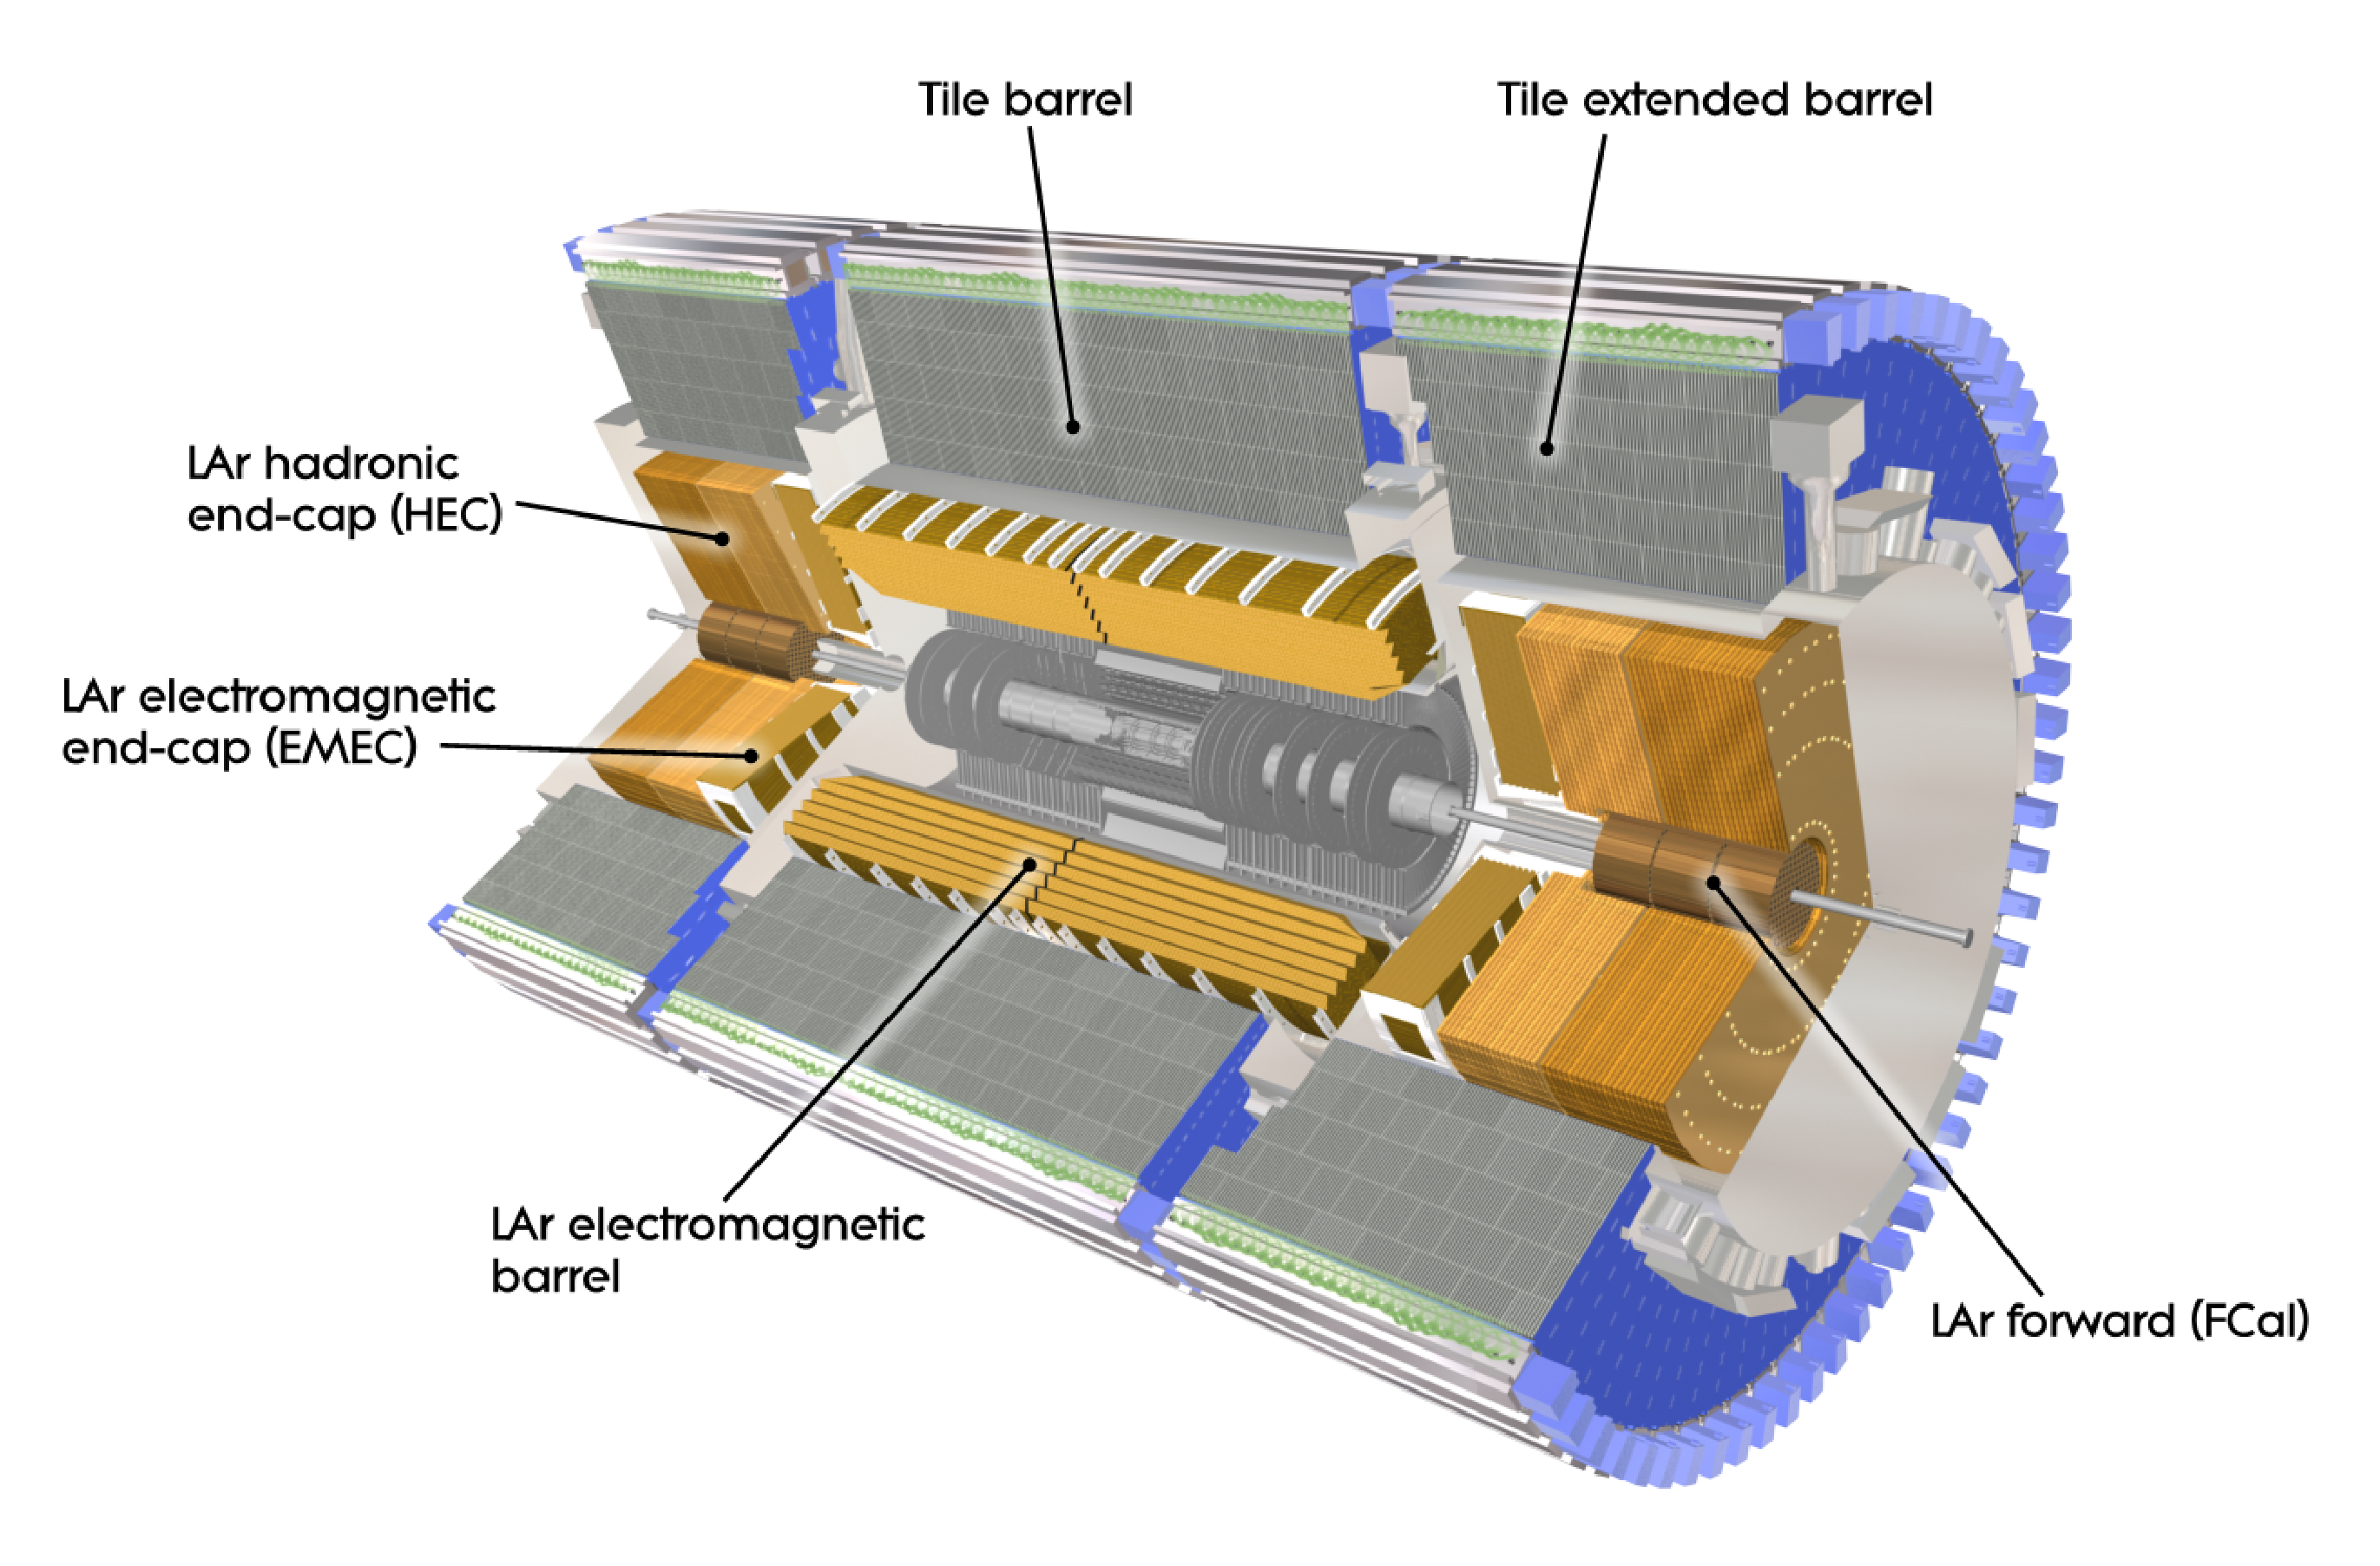
\includegraphics[width=0.8\linewidth,angle=0]{Detector/calorimeters}
\end{center}
%\centerline{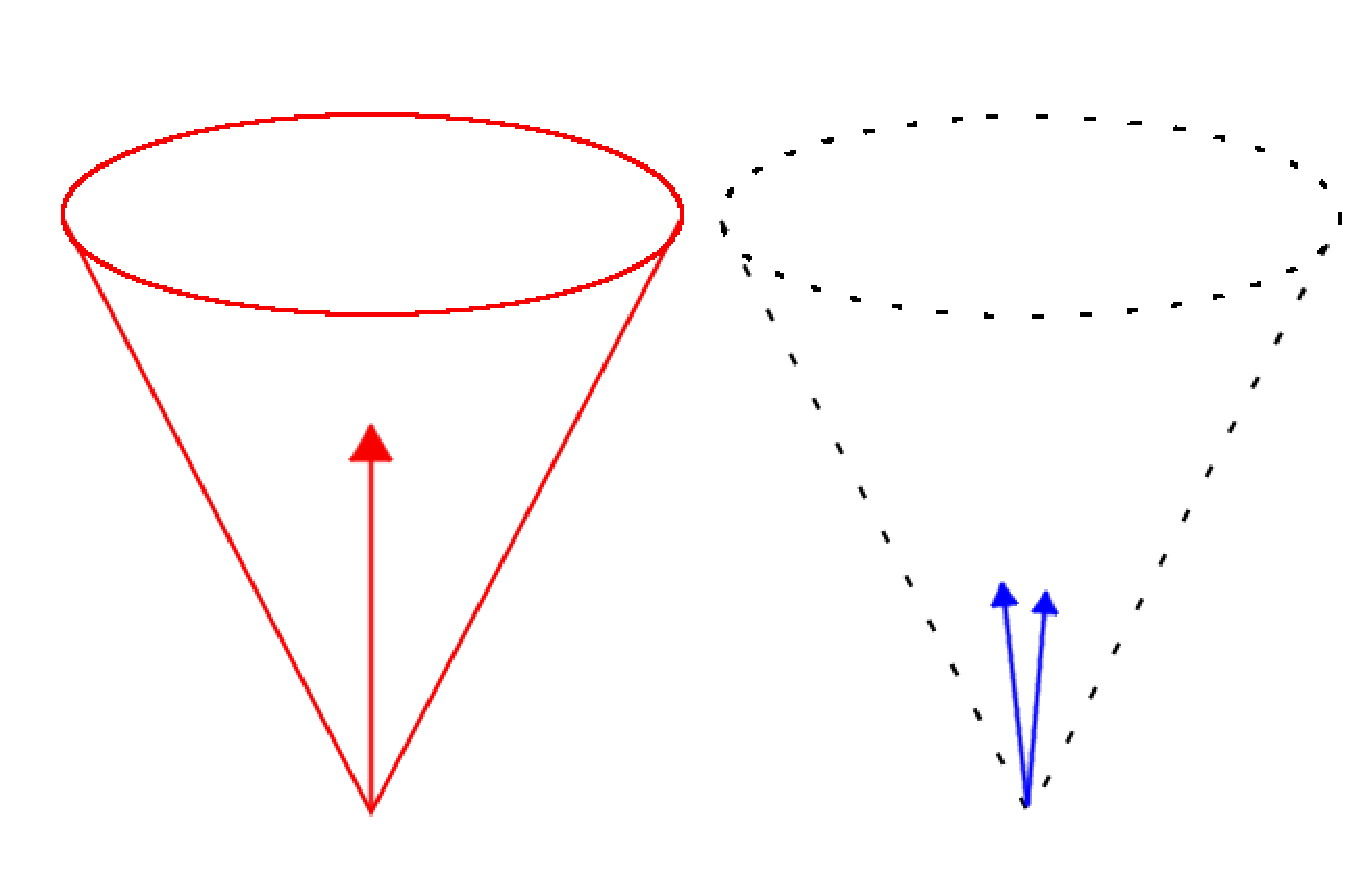
\epsfig{file=./figs/collinear.eps  , width=0.95\textwidth}}
\caption{The calorimeters of the ATLAS detector.}
\label{fig_calorimeters}
\end{figure}
\subsubsection{Barrel Calorimeters}
%\red{All these calorimeters use liquid argon as the active detector medium; liquid argon has been chosen for its intrinsic linear behaviour, its stability of response over time and its intrinsic radiation-hardness. }

%\red{ok, need to discuss why LAr is used, and why its accordion shaped}
%The EM Barrel (EMB) calorimeter is a lead/liquid argon calorimeter covering the ps with a distinctive accordion-shaped geometry. 
%
%
%It is made up of two half barrel sections ($z < 0$ and $z > 0$), each divided azimuthally into 16 modules. It covers the pseudorapidity range $0< |\eta| < 1.475$, and is completely symmetric in $\phi$.

% consists of three layers, plus presampler. 
The EMB calorimeter is a lead/liquid argon sampling calorimeter covering the pseudorapidity range $|\eta| < 1.475$. Liquid argon \cmt{(LAr)} was chosen for the active medium because it can be used to obtain a fast, linear response while also being resistant to radiation~\cite{detector_paper}. The absorber plates are folded into a distinctive accordion shape, as shown in Figure ~\ref{fig_EMB_section}. The shape of the absorber plates gives the EMB calorimeter a structure that is completely symmetric in the azimuthal direction, with no gaps in detector coverage. The linearity and resolution of the response are thus uniform in $\phi$.


%The absorber plates are made of lead, and are 1.5mm thick for $|\eta| < 0.8$ and 1.1 m thick for $|\eta| > 0.8$.  

The absorber plates are made of lead, with stainless steel sheets glued on each side in order to increase their mechanical strength. The plates are then folded into the accordion shape, with the folding angle increasing with depth (radius) in order to maintain the size of the LAr gap (and hence the sampling fraction) throughout the calorimeter. The lead plates are 1.5mm thick for $|\eta| < 0.8$ and 1.1 m thick for $|\eta| > 0.8$. Thinner sheets are used at higher $|\eta|$ in order to control the depth of the calorimeter\cite{TDR_LAR}, which varies from 22 - 30 $X_0$ in the region $0 < |\eta|<0.8$, and from 24 to 33 $X_0$ in the region $0.8 < |\eta|<1.3$. 

%The depth of the calorimeter increases with $\eta$, as particles at higher values of $\eta$ will travel a longer distance in order to traverse the same radial depth. 
% 
%
%change thickness, reduces depth. More LAr, so better response/resolution
%
%
% An 0.2mm sheet of stainless steel is glued onto each side of the lead plate in order to increase the mechanical strength of the absorber sheets. These sheets are then folded into the accordion shape. The folding angle increases with depth (radius) in order to maintain the size of the LAr gap throughout the calorimeter. 

%, which is 2.1mm on either side of the electrodes.
\begin{figure}[tb]
\begin{center}
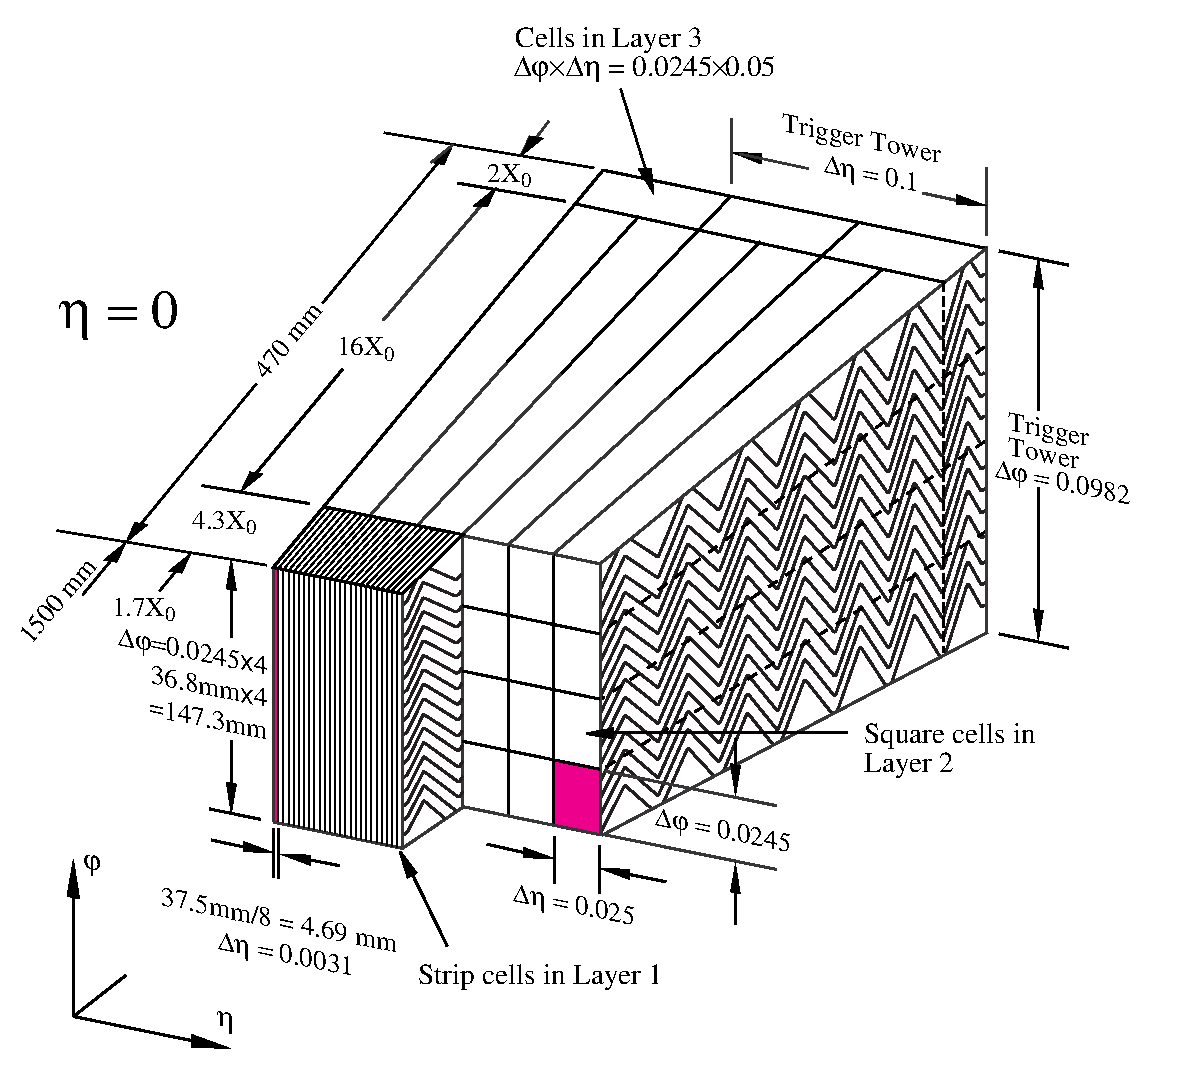
\includegraphics[width=0.5\linewidth,angle=0]{Detector/EMB_section}
\end{center}
%\centerline{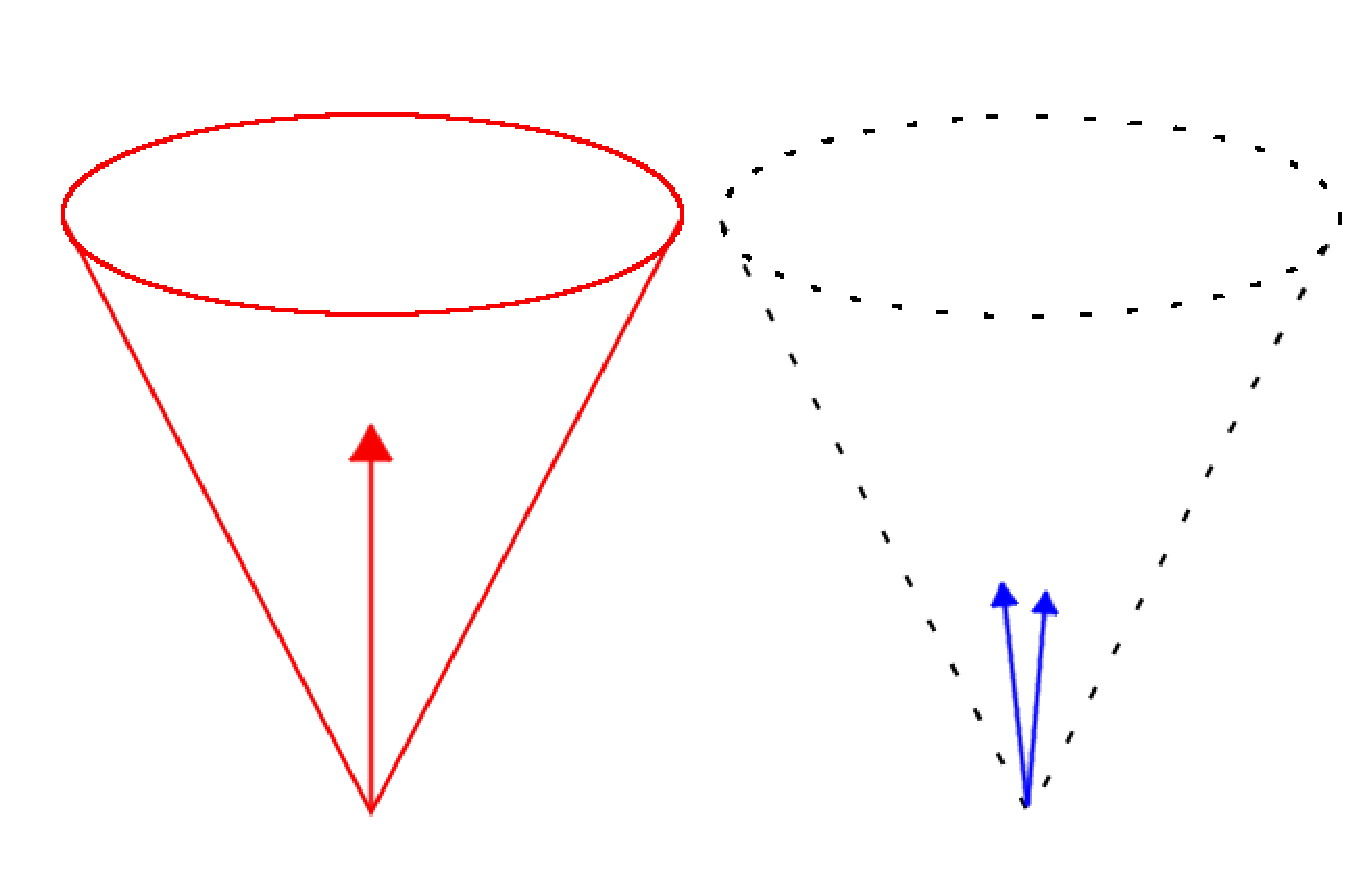
\epsfig{file=./figs/collinear.eps  , width=0.95\textwidth}}
\caption[Section of the EMB calorimeter]{Section of the electromagnetic barrel calorimeter, showing the accordion shape of the absorber plates.}
\label{fig_EMB_section}
\end{figure}

Flexible Printed Circuit Boards (PCBs) are used to form the electrodes, which consist of three layers of copper separated by polyimide. The electrodes are positioned in between layers of the absorber, with honeycomb spacers being used to keep the electrodes in the centre of these gaps. The absorber layers are grounded, while the two outer layers of copper on each electrode are connected to an HV supply at +2kV~\cite{detector_paper}. This creates two active liquid argon gaps of thickness 2.1 mm on either side of the electrode. The inner layer of copper on each electrode is used to read out the signal, as it is capacitively coupled to both the outer layers.


The readout of the EM Barrel calorimeter~\cite{ATLAS_barrel_electrode} is divided longitudinally (i.e. in depth) into three layers. The first and third layers are each a few $X_0$ in depth and only contain the beginning and end of the shower, while most of the energy is deposited in the second layer which has a depth of $\sim$17-20 $X_0$. The readout granularity in $\Delta \eta \times \Delta \phi$ is 0.003 $\times$ 0.1, 0.025 $\times$ 0.0245, and 0.05 $\times$ 0.0245 in layers 1, 2 and 3, respectively. A diagram of the readout layer of the electrode is shown in Figure~\ref{fig_EMB_electrode}, in which the different readout granularities are visible. The first layer has a very fine segmentation in $\eta$, which allows decaying $\pi^0$ particles to be distinguished from individual photons.\cmt{cite tdr}

\begin{figure}[tb]
\begin{center}
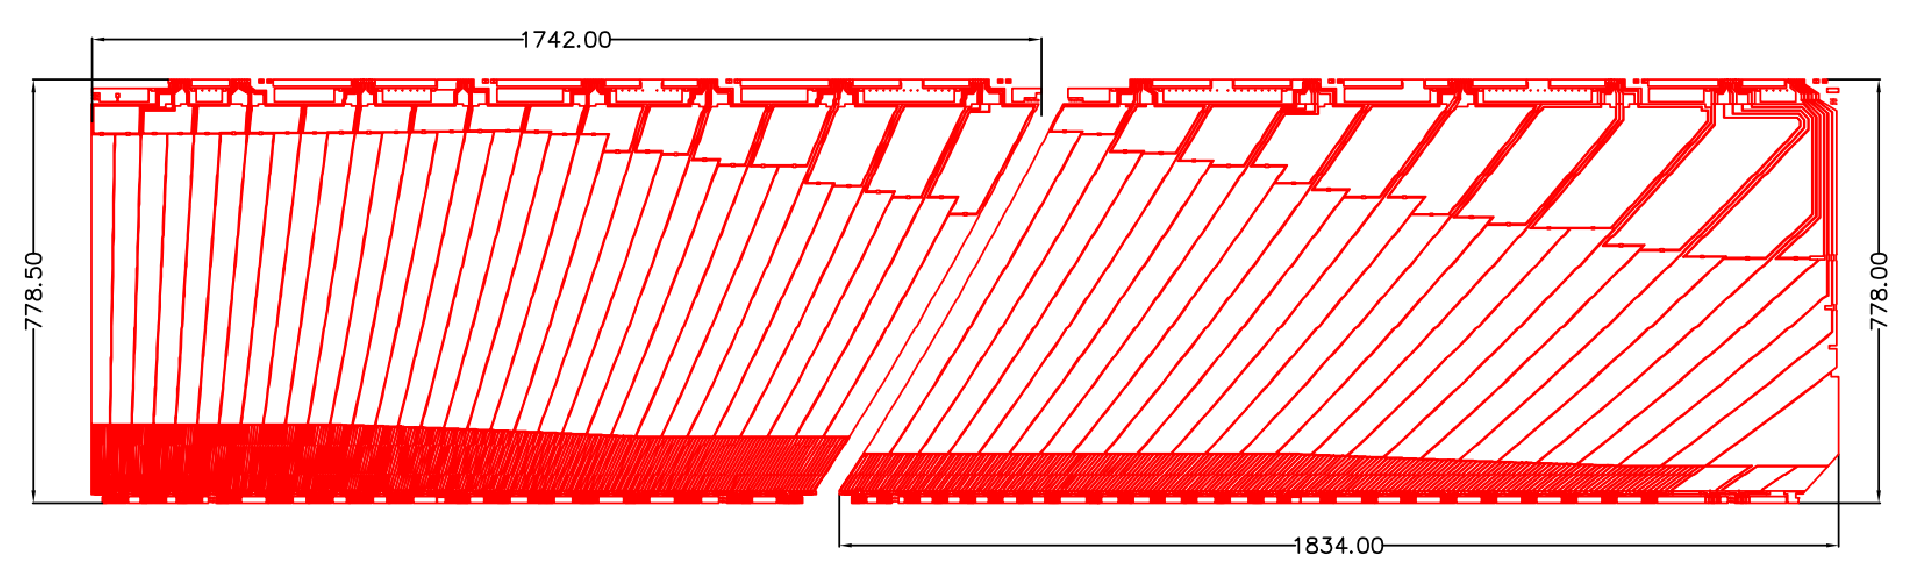
\includegraphics[width=0.95\linewidth,angle=0]{Detector/EMB_electrode}
\end{center}
%\centerline{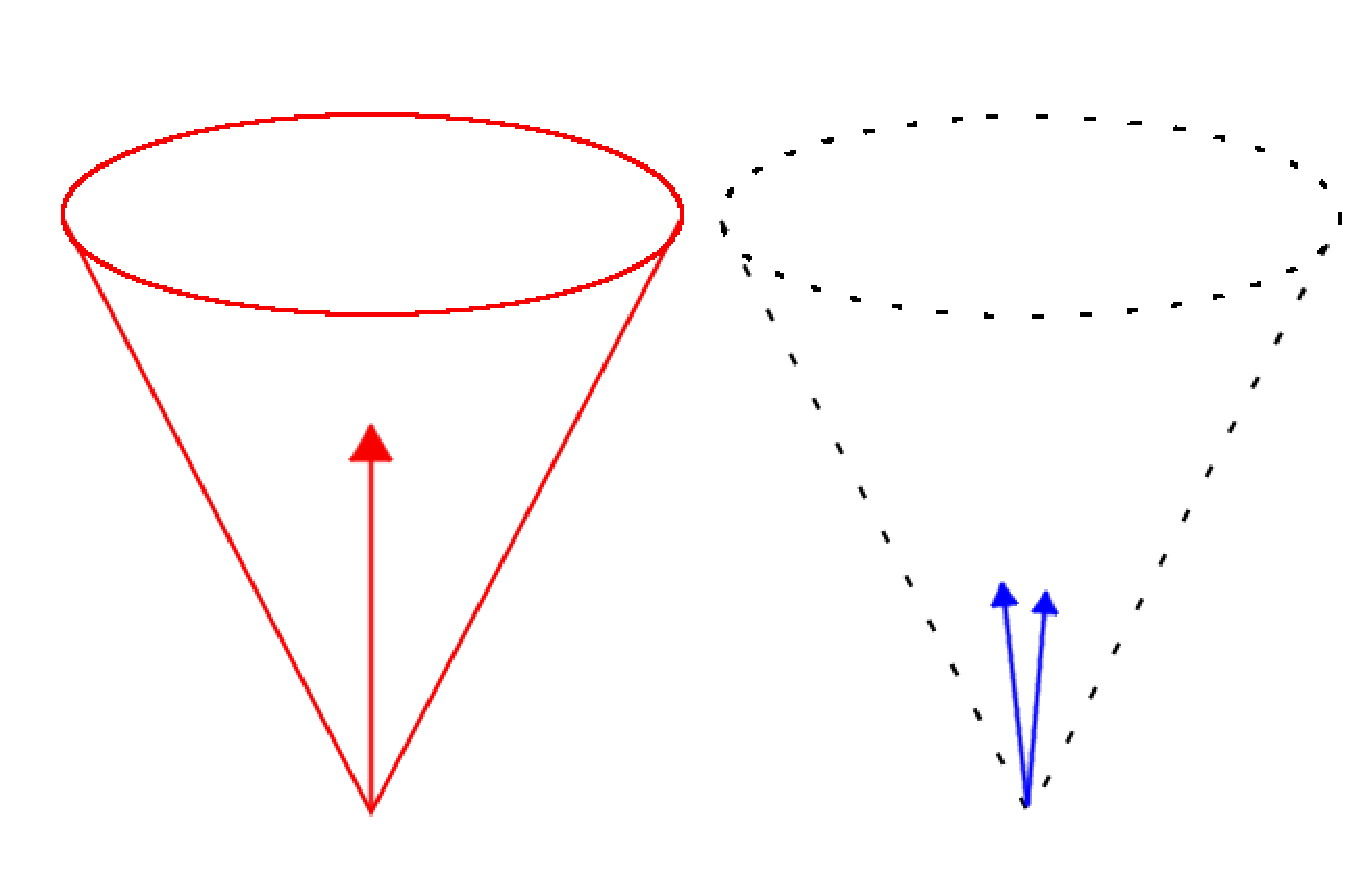
\epsfig{file=./figs/collinear.eps  , width=0.95\textwidth}}
\caption[Readout layer of EMB electrode]{Schematic view of the readout layer of an EM Barrel electrode, prior to folding. The piece on the left is used to read out signals from $0 < \eta < 0.8$, while the piece on the right covers the region $0.8 < \eta < 1.475$~\cite{ATLAS_barrel_electrode}.}
\label{fig_EMB_electrode}
\end{figure}






%TILE
%\red{The choice of this technology provides maximum radial depth for the least cost for ATLAS}
A steel/scintillator ``Tile'' calorimeter~\cite{ATLAS_TILE_TDR} is used to measure the energy of hadronic particles in the barrel region. It consists of a central barrel section covering the pseudorapidity range $|\eta| < 0.8$, and two extended barrel sections that enclose the LAr end-caps. 
The Tile calorimeter receives less radiation than the EM Barrel, and so alternatives to liquid argon based calorimetry are viable in this region. A steel/scintillator calorimeter was chosen as it was the most cost effective way of building a hadronic calorimeter with a large depth\cite{detector_paper}. The total depth of the Tile calorimeter is about 7.4 interaction lengths.

Each section of the Tile calorimeter is divided into 64 modules, each of which covers an azimuthal angle of $5.625^\circ$.
The absorbing material of the calorimeter is formed from a series of steel ``master'' plates, which are 5mm thick and run the full radial depth of the Tile calorimeter (2.0m). A series of smaller, 4mm thick spacer plates are positioned in between layers of master plates. The spacer plates are used to create gaps between adjacent master plates, and it is within these gaps that the scintillating tiles are located, as shown in Figure~\ref{fig_tile_module}.
\begin{figure}[tb]
\begin{center}
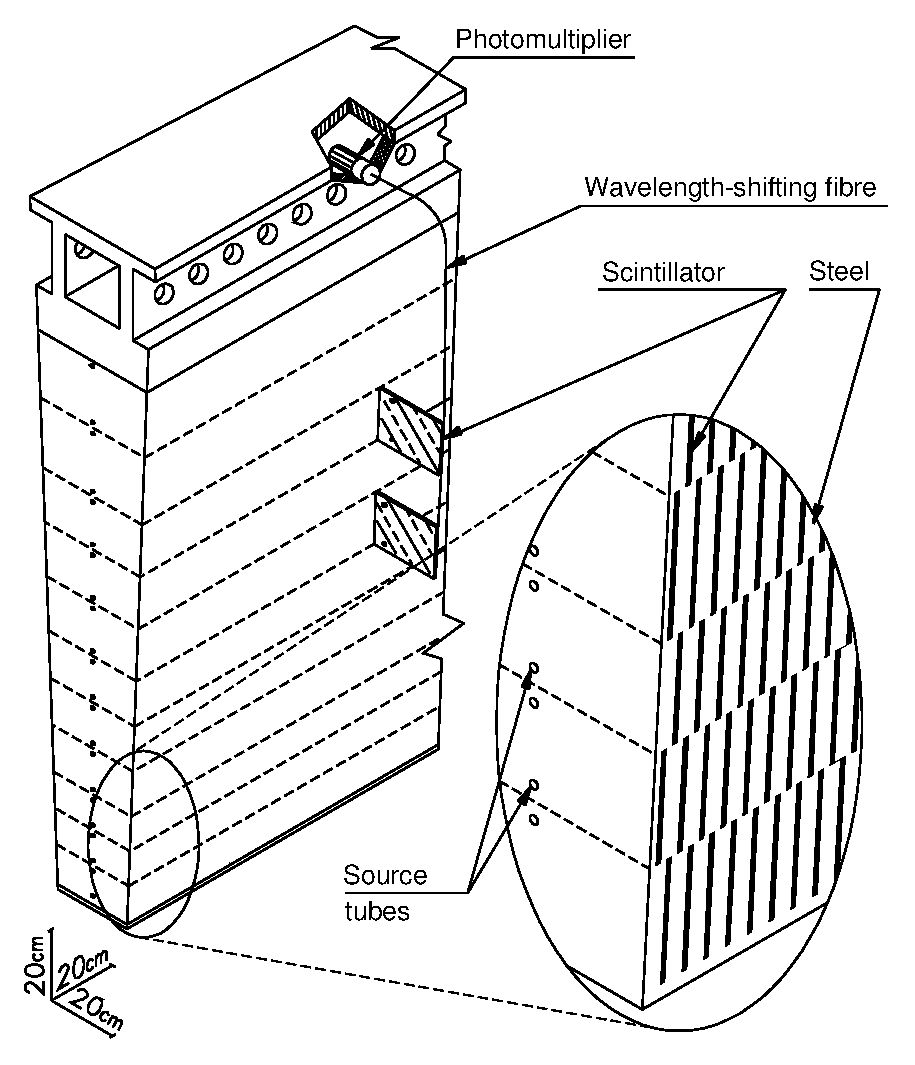
\includegraphics[width=0.5\linewidth,angle=0]{Detector/TileCal_Module3}
\end{center}
%\centerline{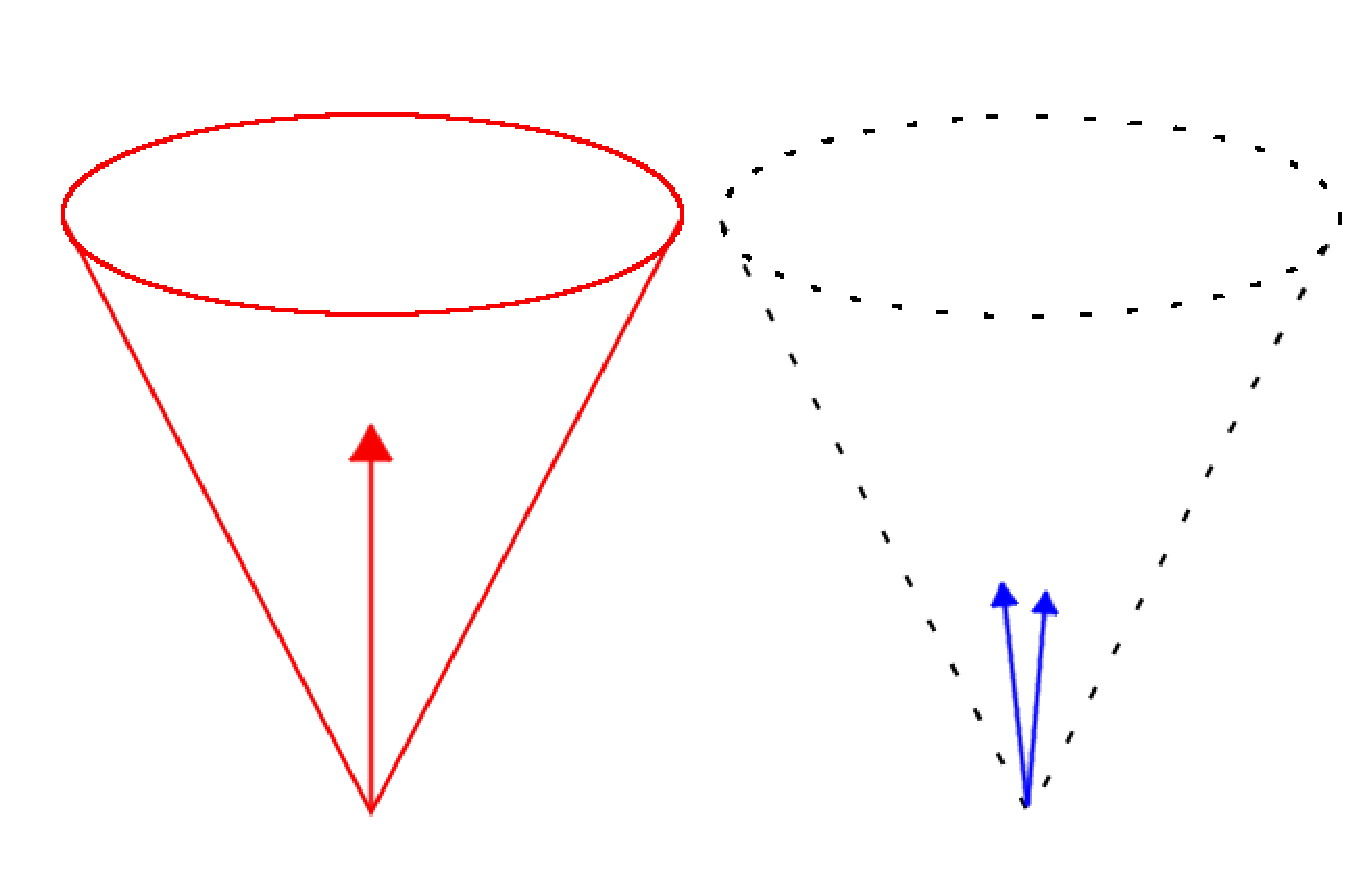
\epsfig{file=./figs/collinear.eps  , width=0.95\textwidth}}
\caption[Schematic of a tile calorimeter module]{Schematic of a tile calorimeter module. Alternating layers of master plates and spacer plates are glued together, with scintillating tiles positioned in the gaps in this structure.}
\label{fig_tile_module}
\end{figure}
The scintillating tiles are made of polystyrene, which produces scintillation light in the ultra-violet range when excited by the passage of showering particles. The polystyrene is doped with fluors that shift the wavelength of this light into the visible spectrum. Optical fibres are coupled to two sides of each scintillator tile, and are used to carry light from the tiles to the Photomultiplier tubes (PMTs), which are housed within the mechanical support structure of the calorimeter. The PMTs then convert the scintillation light to an electronic signal.


%central barrel (5.8 metres long) and two extended barrel regions that are located outside the end-caps
%
%has a depth of $\sim 7.4 \lambda$.
%
%
%
%tile steel/scintillator
%scintillators are polystyrene based, scintillation light is UV, but polystyrene doped with wavelength shifting fluors that move the wavelength into the visible spectrum.

\subsubsection{End-Cap Calorimeters}

The Electromagnetic End-Cap  (EMEC) and Hadronic End-Cap (HEC) Calorimeters are liquid argon calorimeters housed within the end-cap cryostats at either end of the detector.

The EMEC covers the pseudorapidity range $1.375 < |\eta| < 3.2$, and has a similar design to the EM Barrel calorimeter. As with the barrel, the absorber is formed from accordion shaped layers of lead sheets, while the active regions consist of the liquid argon gaps between these layers. Honeycomb spacers are used to keep the electrodes positioned in the centres of these gaps. A module of the EMEC is shown in Figure~\ref{fig_EMEC_module}.

The EMEC consists of two coaxial wheels, with the boundary between wheels located at $|\eta| = 2.5$, matching the acceptance of the ID. The inner wheel uses absorber sheets of thickness 2.2mm, giving the calorimeter a depth of $26 - 36 X_0$ in the region $2.5 < | \eta| < 3.2 $, while the absorber plates in the outer wheel are thinner (1.7mm) giving the calorimeter a depth of $24 -34 X_0$ in this region. Each wheel is subdivided into eight wedge-shaped modules. Due to the accordion shape of the absorber layers, there are no discontinuities in the calorimeter between adjacent modules. As with the EM barrel, the structure of the EMEC is completely symmetric with respect to azimuthal angle. The number of readout layers and their granularities are dependant on pseudorapidity; this information is summarised in Table~\ref{table_gran_emec}. 

\begin{figure}[tb]
\begin{center}
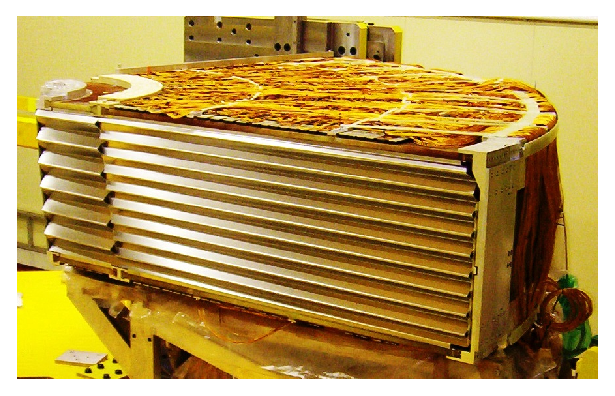
\includegraphics[width=0.8\linewidth,angle=0]{Detector/EMEC_module}
\end{center}
%\centerline{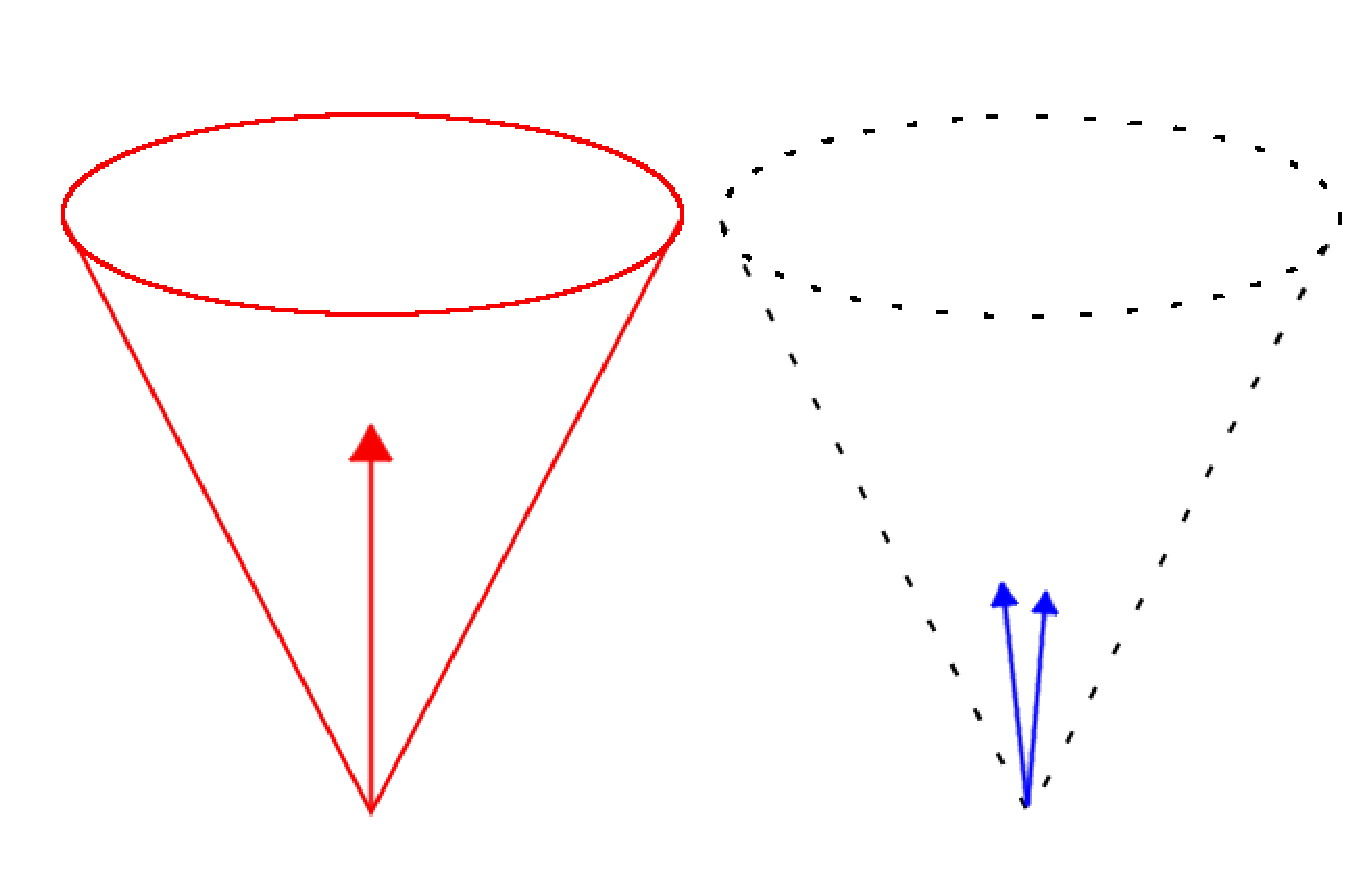
\epsfig{file=./figs/collinear.eps  , width=0.95\textwidth}}
\caption[Photograph of an EMEC module.]{photograph of an EMEC module, showing the accordion structure of the absorbers. The boundary between the inner wheel and the outer wheel can be seen towards the left, where the shape of the absorber plate changes.}
\label{fig_EMEC_module}
\end{figure}

\begin{table}[!htbp]
\begin{center}
\begin{tabular}{|l|l|l|l|}
\hline
pseudorapidity & layer 1 & layer 2& layer 3\\
\hline
$1.375 < |\eta| < 1.425$ &  $0.050 \times 0.1$ & $0.050 \times 0.025$ & \multirow{2}{*}{-} \\
\cline{1-3}
$1.425 < |\eta| < 1.5$ & $0.025 \times 0.1$    & \multirow{5}{*}{$0.025 \times 0.025$} & \\
\cline{1-2} \cline{4-4}
$1.5 < |\eta| < 1.8$ &   $0.0031 \times 0.1$   & &\multirow{4}{*}{$0.050 \times 0.025$} \\
\cline{1-2}
$1.8 < |\eta| < 2.0$ &  $0.0042 \times 0.1$    & & \\
\cline{1-2}
$2.0 < |\eta| < 2.4$ &  $0.0063 \times 0.1$    & &\\
\cline{1-2}
$2.4 < |\eta| < 2.5$ &  $0.025 \times 0.1$     & &\\
\hline
$2.5 < |\eta| < 3.2$ &  $0.1 \times 0.1$       & $0.1 \times 0.1$ & - \\
\hline
\end{tabular}
\end{center}
\caption[Readout granularity for the EMEC]{Readout granularity for the EMEC~\cite{detector_paper}, expressed as $\Delta \eta \times \Delta \phi$.}
\label{table_gran_emec}
\end{table}




% The inner wheel ($2.5 < | \eta | < 3.2$) consists of two layers, both of which have granularity $\Delta \eta \times \Delta \phi = 0.1 \times 0.1$. The inner part of the outer wheel ( $1.5 < |\eta| < 2.5$) consists of three layers, with the second layer having a granularity of $0.025 \times 0.025$ and the third having a granularity of $0.05 \times 0.025$. The granularity of the first layer increases from $\sim 0.003 \times 0.1$ at $|\eta| = 1.5$ to $0.025 \times 0.1$ at $|\eta| = 2.5$. 
%
%thickness of lead in inner and outer wheels.
%
%The readout of inner wheel has a granularity of $0.1 \times 0.1$ in $\Delta \eta \times \Delta \phi$. The granularity of the outer wheel varies with pseudorapidity, but is at its finest ($0.003 \times 0.1$) in the region $ 1.5 < | \eta | < 1.8$.
%\red{more detail about layers, granularity}







%HEC

%\red{why copper?}
The HEC calorimeters~\cite{HEC_construction} utilise a parallel plate geometry, which consists of alternating layers of copper and liquid argon oriented at right angles to the beam. Each side of the HEC consists of front wheel and a rear wheel, each of which is divided azimuthally into 32 wedge-shaped modules. The front wheel is comprised of a front plate which is 12.5 mm thick, as well as 24 copper plates, each of which is 25mm thick. The rear wheel contains a front plate that is 25mm thick, and is followed by 16 plates of thickness 50mm. 

In both wheels, the liquid argon gaps formed between the absorber plates have a depth of 8.5mm. These gaps are divided into four sub-gaps of thickness $\sim$2mm by a set of three parallel electrodes, forming an electrostatic transformer~\cite{1990NIMPA}. This makes it easier to match the impedance of the calorimeter channel to the readout electronics. The signal is read off a central pad in the middle electrode, with shapes etched into these pads determining the read-out structure. Cells in the HEC have a granularity of 0.1 $\times$ 0.1 in $\Delta\eta \times\Delta\phi$ for $|\eta| < 2.5$, and  0.2 $\times$ 0.2 at higher $|\eta|$.
%\red{why copper?}

\begin{figure}[tb]
\begin{center}
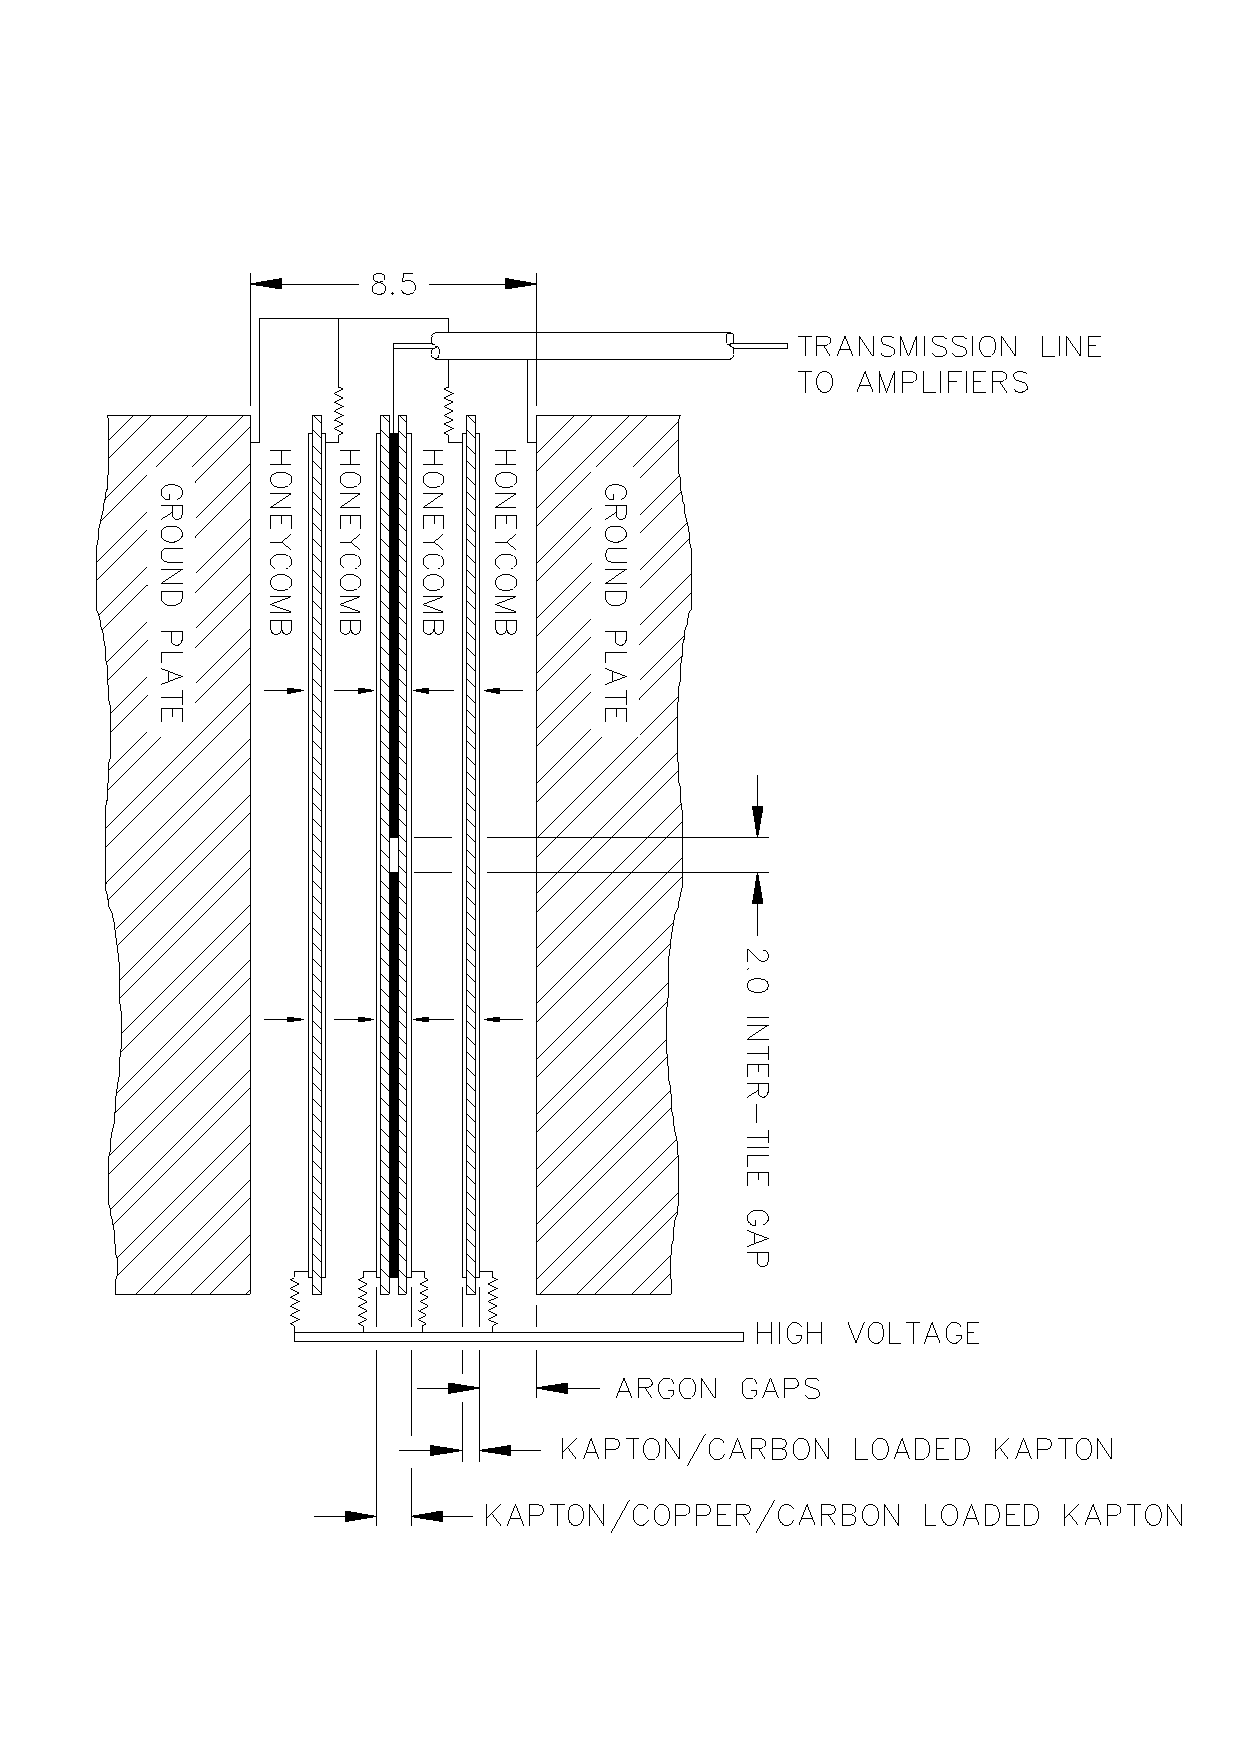
\includegraphics[width=0.5\linewidth,angle=0]{Detector/HEC_estM}
\end{center}
%\centerline{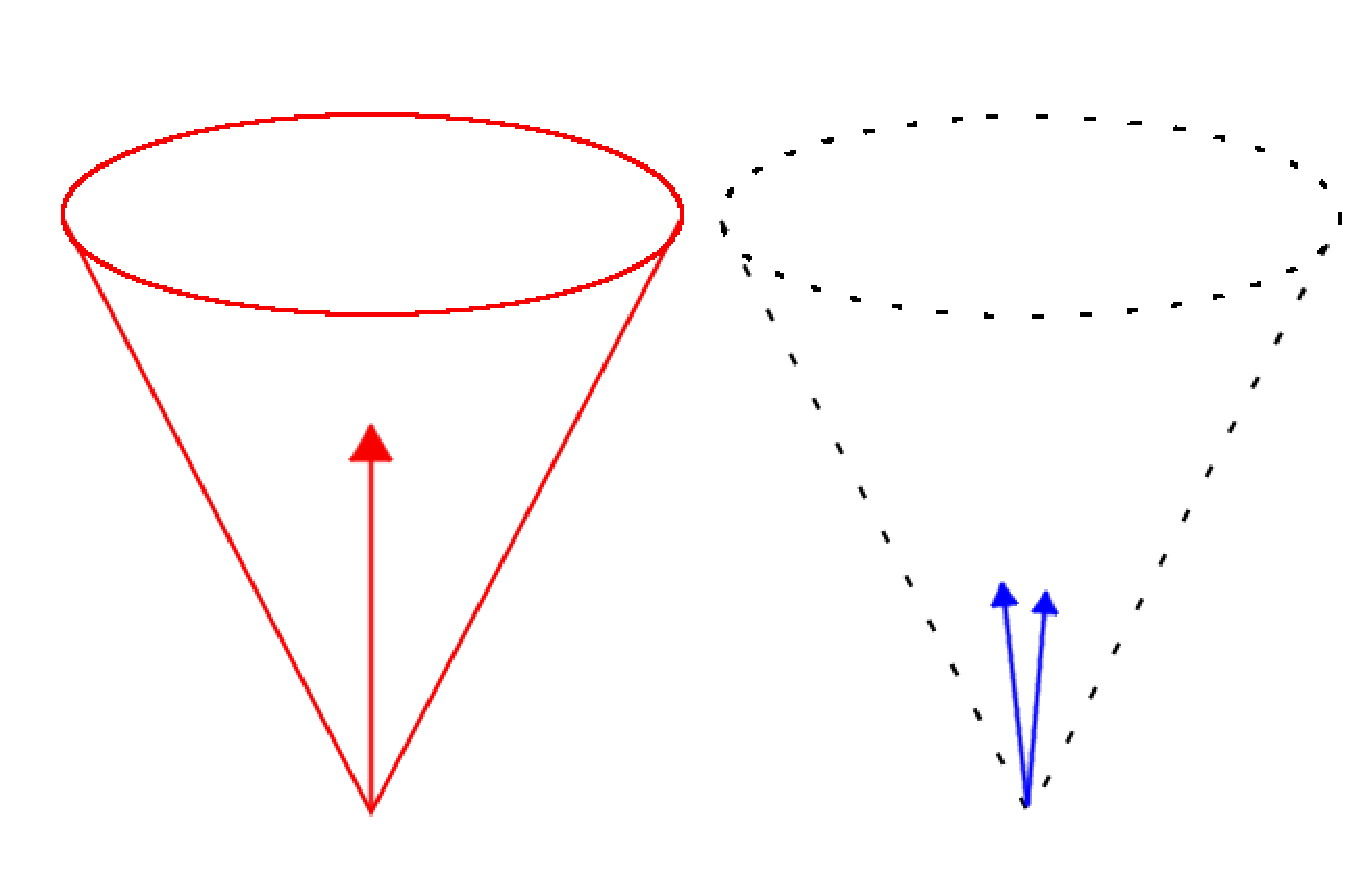
\epsfig{file=./figs/collinear.eps  , width=0.95\textwidth}}
\caption[Electrode structure in the HEC]{Electrode structure in the HEC. Electrodes are arranged to form an electrostatic transformer}
\label{hec_electrode_fig}
\end{figure}
%Central plate used to read out signal, readout structure is embedded/etched on this plate. granularities.
%
%
%Each gap is divided into 
%
% 
%HEC,  cu / LAr
%
%hec consists of two wheels, Hec 1 and Hec2, each wheel has two longitudinal sections
%
%made of alternating layers of Cu and LAr. Cu consists of flat plates normal to the beam.



%%Em barrel
%rapidity range (central barrel, extended barrel - tile)
%
%
%Tile
%
%End cap (EMEC/HEC)



%Tile
%
%LAR
%EM barrel
%EMEC
%HEC
%\clearpage
\subsection{Forward Calorimeters}
\label{chap_Detector_FCal}
%Be Consistent - specify cold dimensions

%figures to add:
%FCal in support tube
%electrode with tungsten slugs



The \atlas Forward Calorimeters (FCal) are located just outside the beampipe, with their front faces situated 4.7~m on either side of the \atlas interaction point. These are liquid argon based calorimeters, and are located within a support tube inside the end-cap cryostat (Figure~\ref{fig_cut}). They cover the pseudorapidity region $3.1 < |\eta| < 4.9$.

\begin{figure}[tb]
\begin{center}
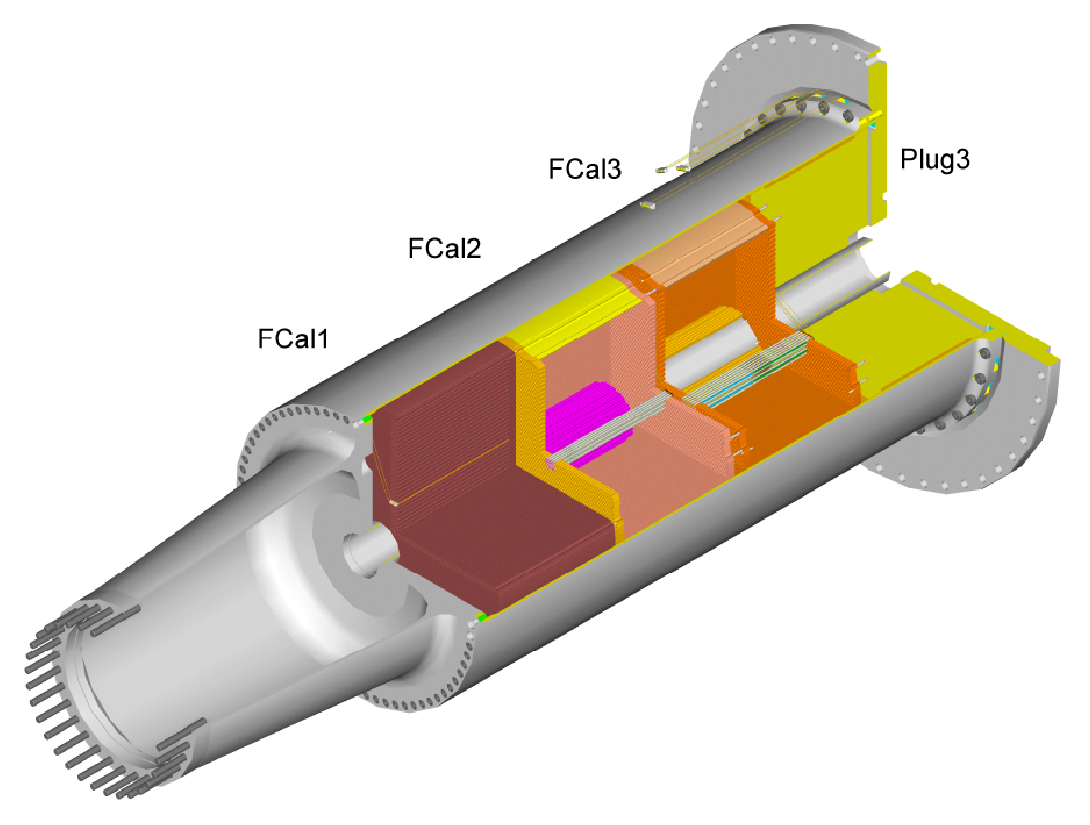
\includegraphics[width=0.8\linewidth,angle=0]{TBoverview/FCal_support_cutaway.eps}
\end{center}
%\centerline{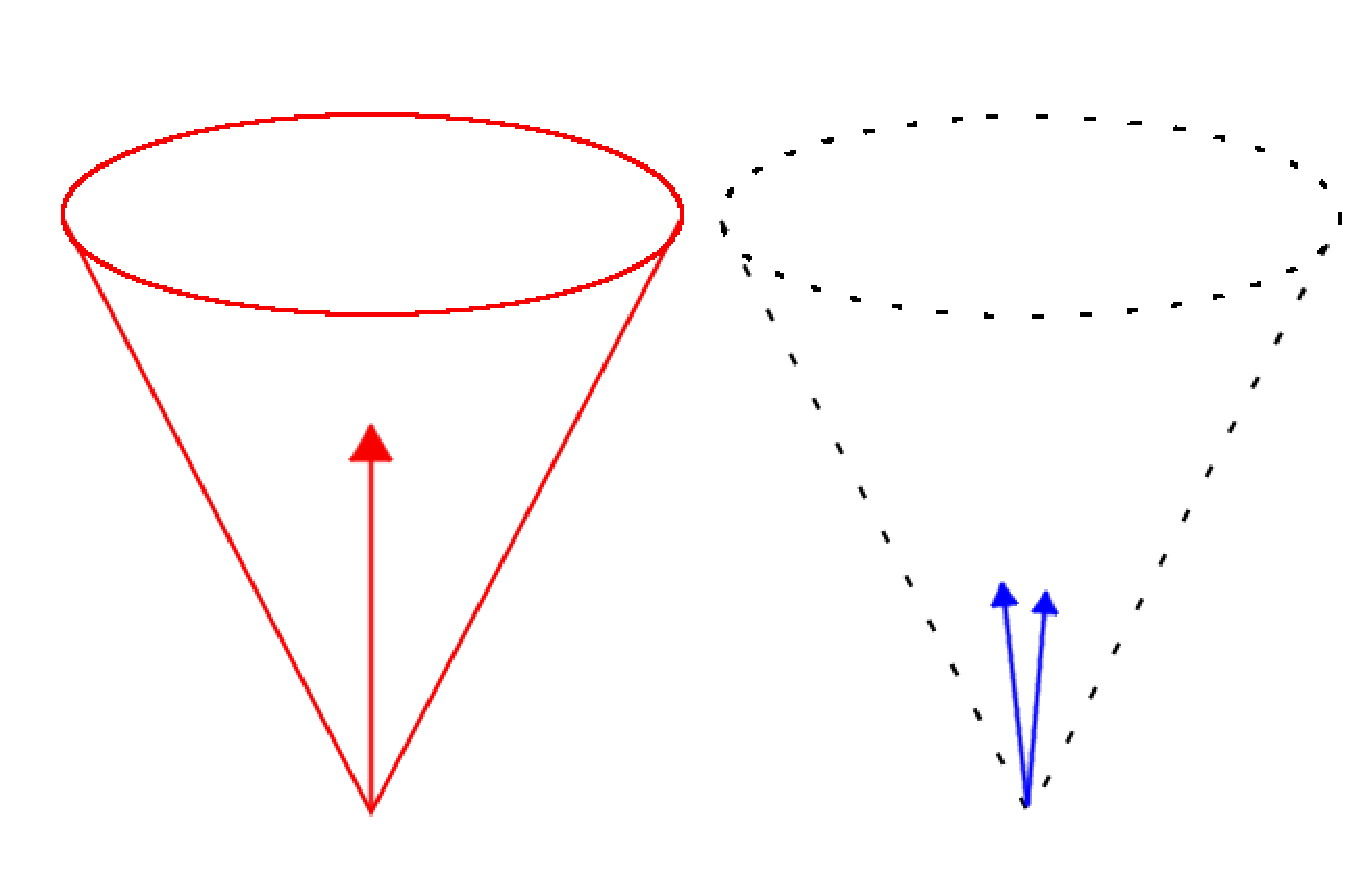
\epsfig{file=./figs/collinear.eps  , width=0.95\textwidth}}
\caption[Cut-away view showing the FCal within its support tube]{Cut-away view showing the FCal within its support tube\cite{FCal_jinst_2010}. The region inside the support tube and just upstream of the calorimeter is evacuated in ATLAS.}
\label{fig_cut}
\end{figure}


Each FCal consists of three modules, one electromagnetic module (FCal1) and two hadronic modules (FCal2 and FCal3). Each module has a cylindrical shape, with an outer radius of 449~mm and a depth of 444~mm. A plug made of a brass alloy has a similar shape and is located behind the hadronic modules in order to provide additional shielding for the muon chambers behind it. As the FCal operates at a temperature just below 90K in \atlas, ``cold'' values will be used in the following when quoting dimensions, densities, or other temperature-dependent quantities. %\red{ radiation and interaction lengths}.

The electromagnetic modules of the FCal were produced by the University of Arizona. Each module consists of a stack of circular copper plates with an inner radius of 72 mm and an outer radius of 449~mm.\cmt{On the ``A'' side, the FCal 1 module consists of 18 plates of thickness 24 mm, whereas on the ``C'' side 19 slightly thinner plates are used.}  Each plate is drilled with a hexagonal array of holes into which the electrodes were inserted. This was done in a way that established a good electrical connection between the outside of the electrode and one of the copper end-plates. Each electrode consists of a copper tube (the cathode) containing a copper rod (anode) around which a radiation-hard PEEK fibre is wrapped. The inner radius of the copper tubes is 2.62~mm while the radius of the copper rods is 2.35mm, thus leaving a gap of 267~$\mu$m which is filled with liquid argon. The PEEK fibre has a diameter of 250~$\mu$m, and is present to keep the rod positioned in the centre of the tube, thus maintaining the uniformity of the LAr gap throughout the electrode and keeping the rod electrically isolated from the tube. Typical gap sizes used in traditional LAr calorimeters are on the order of a few millimetres, as is the case for the EM Barrel, EMEC and HEC calorimeters. However, as the FCal is located at high pseudorapidity, minimum bias events will deposit energy in it at a very high rate. The smaller gap size is required in order to reduce the drift time across the gap, and thus preventing the high rate of ionisation from causing a build-up of positive ions in the liquid argon. Positive ion buildup can distort the electric field in the LAr gap, thus distorting the signal from the electrode.
The distance between electrodes in FCal1 is similar to the \moliere radius  for copper. EM showers in the FCal should thus spread across several electrodes, allowing the calorimeter to sample the shower effectively. Copper also allows the FCal1 module to conduct heat efficiently. The cryostat temperature is kept at about 88.5K, while the boiling point for liquid argon within the cryostat is 92.7K. With the LHC running at design luminosity, minimum bias events are expected to heat the FCal at a rate of about 45W, with about half of that power going into FCal1. A finite element analysis estimated that this heating would cause a temperature increase within the FCal of no more that 1.5K, which is not enough to cause the liquid argon to boil\cite{FCal_jinst_2010}.

% This is important, as it prevents the energy deposited within the FCal from raising the %temperature of the liquid argon above its boiling point. 
%
%
%%maintained below 90K
%%boils at 92,7K
%
%
%%drift time of 61ns in FCal1, compared to 450 ns for a 2mm gap
%%energy density lower in hadronic modules, so can have a larger gap
%FCal1 28X0 deep, 2.7 lambda
%FCal2 and 3 are 3.6 and 3.7
%
% build up from occurring in the LAr due to  the high rate of ionisation. Moliere radius similar size to electrode spacing

The hadronic modules of the FCal were produced at the University of Toronto (FCal2) and at Carleton University in Ottawa (FCal3). They have a similar design to the electromagnetic module, however tungsten is used as the absorber material instead of copper. Each of the hadronic modules uses two copper end plates drilled with a hexagonal array of holes, each of which holds an electrode. The electrodes use copper tubes for their cathodes and rods made of pure tungsten (with density 19.2 $\mathrm{g}/\mathrm{cm}^3$) for the anodes. The absorber matrix is formed from small slugs of tungsten alloy (``WFeNi'' - 97\% Tungsten/2\% Iron/1\% Nickel) positioned in the gaps between the electrode tubes, as shown in Figure~\ref{slugfig}. The material composition and density of the calorimeter components are important factors when establishing a description of the calorimeter to be used by simulations. By themselves, the WFeNi slugs have a measured mean density of 18.3~$\mathrm{g}/\mathrm{cm}^3$. When considering the WFeNi slugs, the copper electrode tubes, and any spaces in the absorber matrix that are filled with liquid argon, the average density of absorbing material (excluding electrode rods) in the hadronic modules is estimated to be 14.33 $\mathrm{g}/\mathrm{cm}^3$ for FCal2 and 14.45 $\mathrm{g}/\mathrm{cm}^3$ for FCal3~\cite{Archambault:2009zza}. 
%A diagram showing the way in which the WFeNi slugs are positioned amongst the electrodes is shown in figure~\ref{slugfig}

\begin{figure}[tb]
\begin{center}
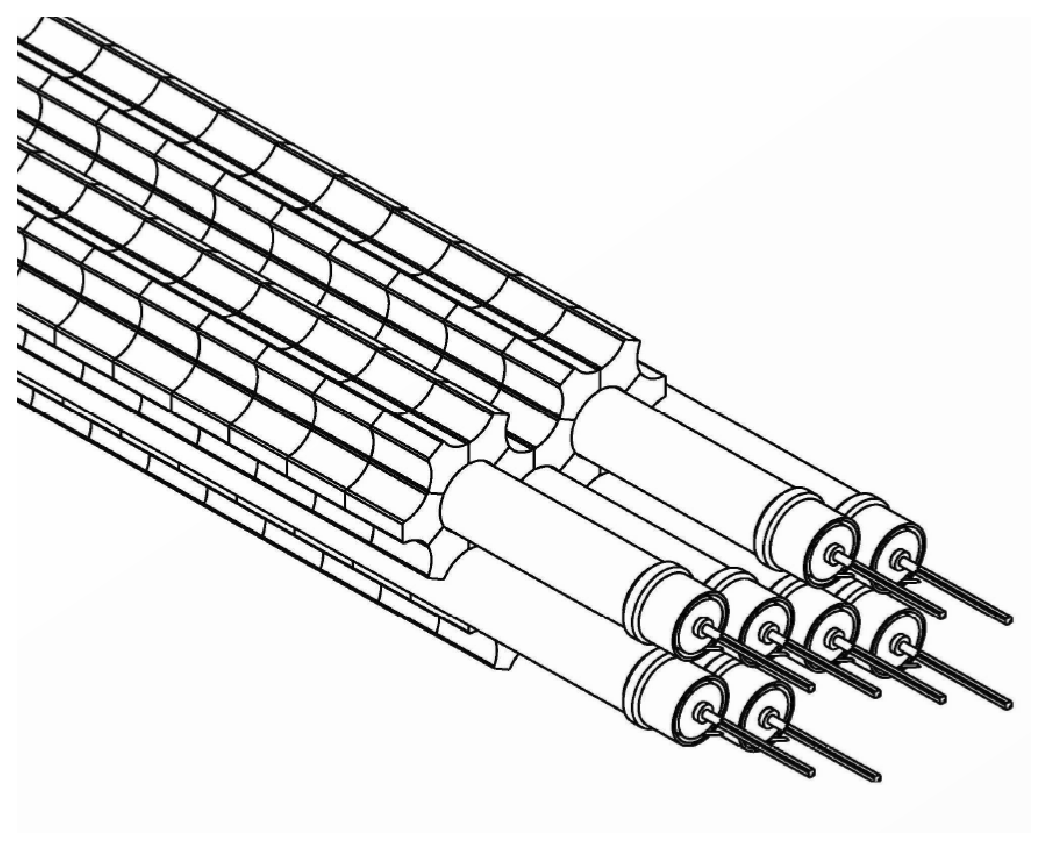
\includegraphics[width=0.5\linewidth,angle=0]{TBoverview/rods_slugs}
\end{center}
%\centerline{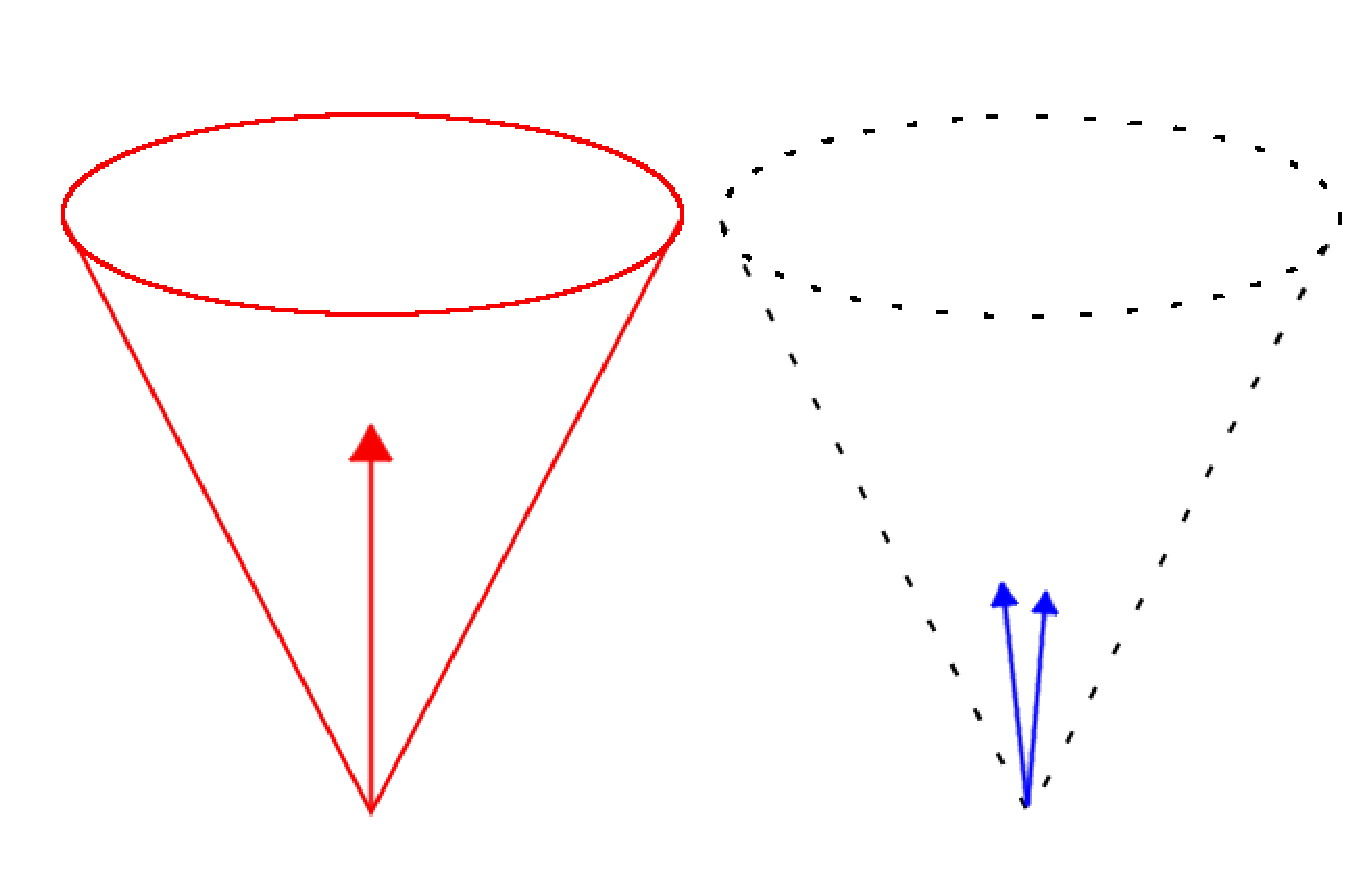
\epsfig{file=./figs/collinear.eps  , width=0.95\textwidth}}
\caption[Electrode/slug arrangement in the FCal.]{Diagram showing the arrangement of electrodes and slugs in the hadronic modules~\cite{FCal_jinst_2010}.}
\label{slugfig}
\end{figure}



%As charge is deposited in the liquid argon, it drifts due to the electric field present in the electrode, causing a current which is used as a signal. The electronics chain used to read out and process this signal is discussed in detail in section~\ref{sec_FCal_electronics}.




%pic of FCal 1/Moliere radius
%pic of FCal in support tube
%pic of FCal2/3 matrix with electrode


%little bit about electronics, which bits are summed, etc.
%dimensions, some photos.
%
%
%table
%module, material, electrode separation, no electrodes, rod diameter, tube inner diameter, lar gap, average absorber density


%rotate the table
%
%\begin{table}[h!bp]
%\begin{center}
%\begin{tabular}{|l|l|l|l|l|l|l|l|}
%\hline
%module & absorber material & module inner diameter & electrode separation & rod diameter & tube  inner diameter & LAr Gap & distance from IP \\
%% module inner radius
%\hline
%\hline
%FCal1 (EM) & Copper & 720 $mm$ & 7.5 $mm$ & 2.35 $mm$ & 2.62 $mm$ & 267 $\mu m$ & 4668.5 $mm$ \\
%\hline
%FCal2 (Had) & Tungsten & 790 $mm$ & 8.2 $mm$ & 2.47 $mm$ & 2.84 $mm$ & 375 $\mu m$ & 5128.3 $mm$\\
%\hline
%FCal3 (Had) & Tungsten & 860 $mm$ & 9.0 $mm$ & 2.75 $mm$ & 3.25 $mm$ & 500 $\mu m$ &  5602.8 $mm$\\
%\hline
%\end{tabular}
%\end{center}
%\caption{Dimensions of the FCal modules.}
%\end{table}
%
%
%
\begin{table}[tb]
\begin{center}
\begin{tabular}{|l|l|l|l||}
\hline
Quantity & FCal1 & FCal2 & FCal3 \\
\hline
\hline
Absorber material & Copper & Tungsten & Tungsten\\
\hline
Module inner diameter & 72 mm & 79 mm & 86 mm\\
\hline
Electrode Separation & 7.5mm & 8.62 mm &9.0mm \\
\hline
Rod Diameter & 2.35 mm & 2.47 mm & 2.75 mm\\
\hline
Tube inner diameter & 2.62 mm & 2.84 mm & 3.25 mm \\
\hline 
LAr Gap & 267 $\mu$m & 375 $\mu$m & 500 $\mu$m \\
\hline
Distance from IP to front face & 4668.5mm & 5128.3 mm & 5602.8 \\
\hline
Number of electrodes & $\sim$ 12,000 & $\sim$ 10,000 & $\sim$ 8000 \\
\hline
\end{tabular}
\end{center}
\caption{Dimensions of the FCal modules.}
\end{table}

\subsubsection{FCal Electronics}
\label{sec_FCal_electronics}
%maybe move this to the detector chapter

%
%An electric field of \~ 1KV/mm is desired for liquid argon calorimeters. In The FCal, the rods in each electrode are connected to a high voltage supply while the electrode tubes are grounded. 
%
%In FCal1, Electrodes are ganged together in groups of four. The four rods are connected to an interconnect board which is supplied by a single HV line \red{(coax?)}. 

%The high voltage is supplied to the electrodes through interconnect boards. In FCal1, electrodes are ganged together in groups of four to form a "tube group". The rods from these electrodes are connected to the interconnect board, which is supplied with HV via a coaxial cable. The cable supplying the HV is also used to read out the signal from the calorimeter, and so the signal (a current pulse) from the electrodes are summed together at the interconnect board.


An electric field of  $\sim$1KV/mm is conventional for liquid argon calorimeters. In order to provide this the rods of each electrode are supplied with high voltage while the tubes are grounded. Showering particles ionise the liquid argon, leaving free electrons and $\mathrm{Ar}^+$ ions in the gap. The electric field in the gap then causes this charge to drift resulting in a current pulse. This pulse is triangular in shape, having a fast rise time ($\sim$1 ns) and taking $\sim$61 ns (in FCal1) to return to zero~\cite{FCal_jinst_2010}. The height of the pulse peak depends on the amount of charge deposited in the liquid argon, and is thus proportional to the amount of energy deposited in the liquid argon \footnote{The energy required to ionise an atom of argon is 15.8 eV.}.
 
% Charge is deposited \cmt{liberated?} in the gap as showering particles ionise the liquid argon.
%Showering particles ionise the liquid argon, leaving free electrons and $\mathrm{Ar}^+$ ions in the gap.

 

%In FCal1, electrodes are ganged together in groups of four to form a "tube group". 

\begin{figure}[tb]
\begin{center}
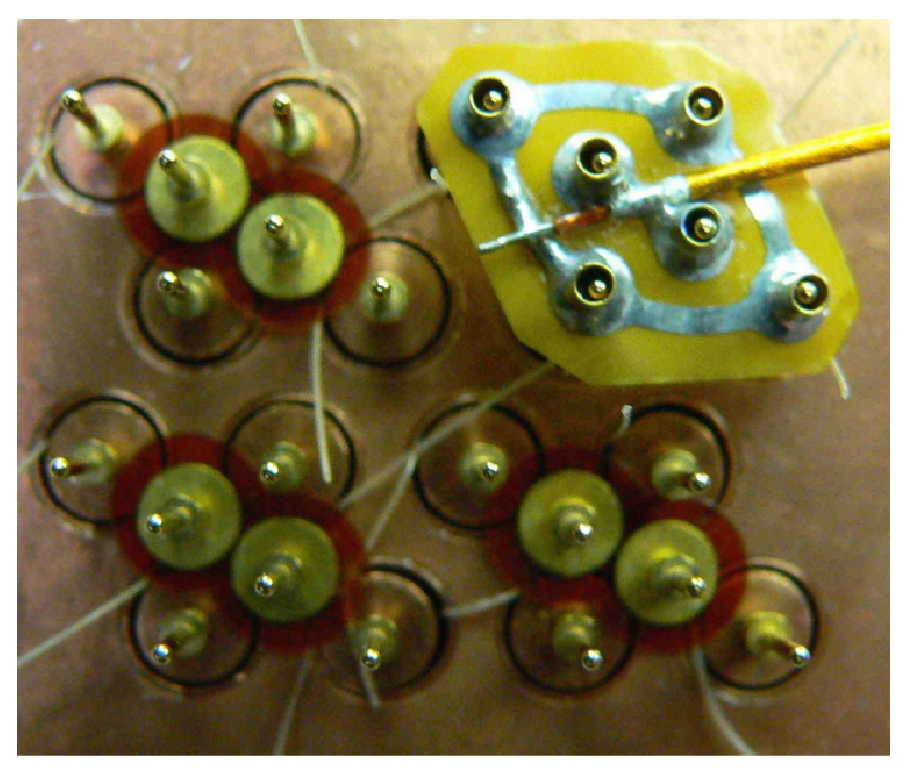
\includegraphics[width=0.6\linewidth,angle=0]{TBoverview/ICB.eps}
\end{center}
%\centerline{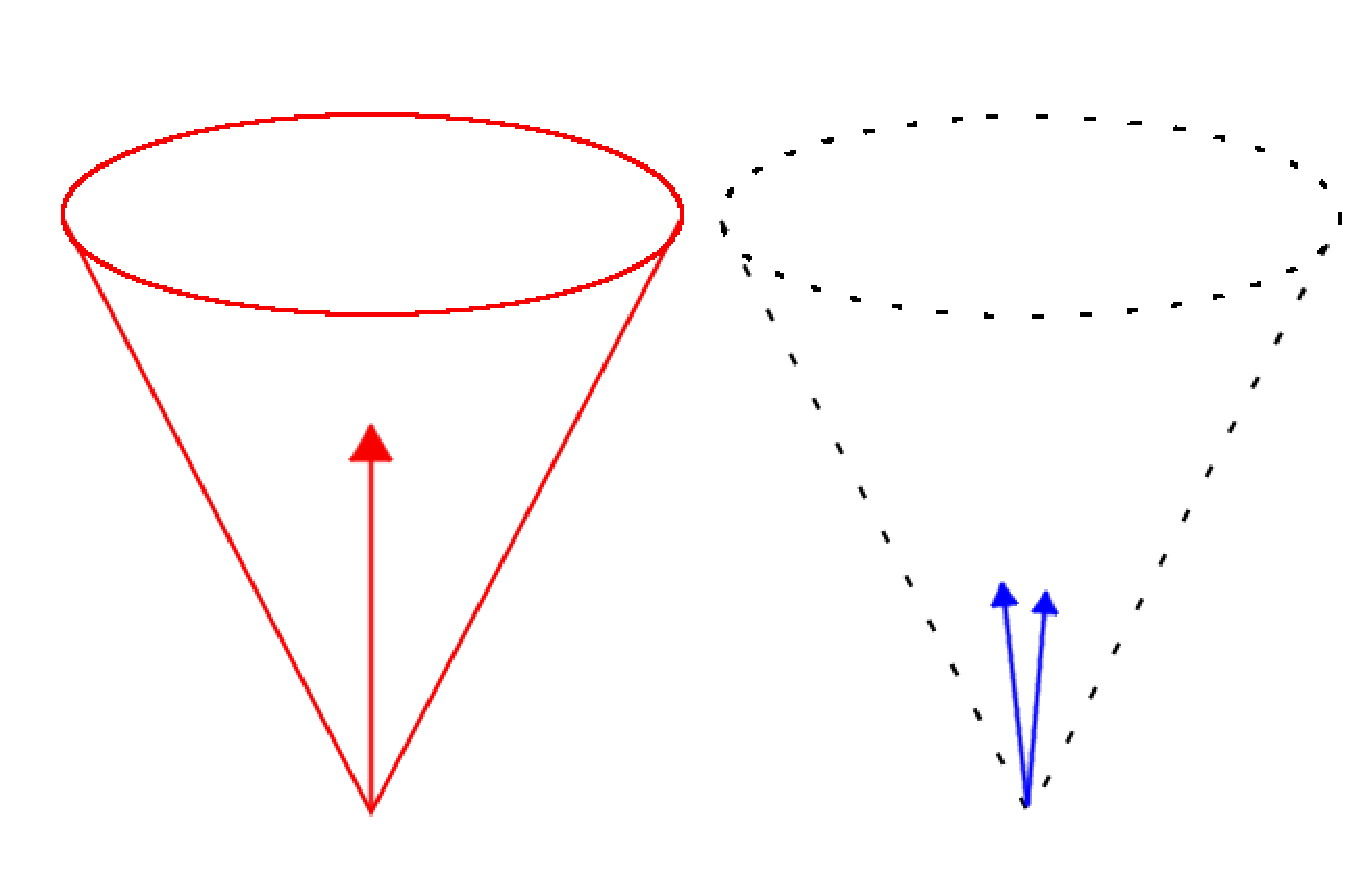
\epsfig{file=./figs/collinear.eps  , width=0.95\textwidth}}
\caption[Photograph of an FCal endplate]{Photo of an endplate of FCal1, taken during assembly, showing the interconnect board and the coaxial cable used for HV delivery and readout~\cite{FCal_jinst_2010}. Also visible are the PEEK fibres used to keep the rods centred within the tubes. The two central pins in each group are used to ground the end plate, and thus the tubes, while the four exterior pins provide HV to the rods and carry the signal off the electrode.}
\label{interconnect_fig}
\end{figure}

The signal is read out via a coaxial cable that also supplies the electrodes with high voltage. Electrodes in the FCal are ganged together on interconnect boards to form ``tube groups''. Tube groups are formed from four electrodes in FCal1, six electrodes in FCal2, and nine electrodes in FCal3. Gold-plated signal pins connect the rods from these electrodes to the interconnect board, which is supplied with HV via a coaxial cable as shown in Figure~\ref{interconnect_fig}. The tubes are also grounded through this coax: each interconnect board is connected (via grounding pins) to the FCal end plate. \cmt{The line supplying HV to the tube group also serves as a readout line, carrying the signal off the interconnect board.}As the interconnect board connects electrodes in parallel, the signal carried off the interconnect board is the sum of the current pulses in each electrode of that tube group.

%As the HV line supplying a tube group is also used to read out the signal, the current pulses from each electrode are summed together on the interconnect board to form one signal for the entire tube group. 

%
%
%
%HV line is also read out line
%
%signal is read off the interconnect board
%
%pulses in all tubes summed on the interconnect board.
%
%
%
%signal read off the interconnect board is the sum of the current pulses in each electrode.

%\blue{Impedance matching (lack of) between electrodes and cable}
 \begin{figure}[tb]
\begin{center}
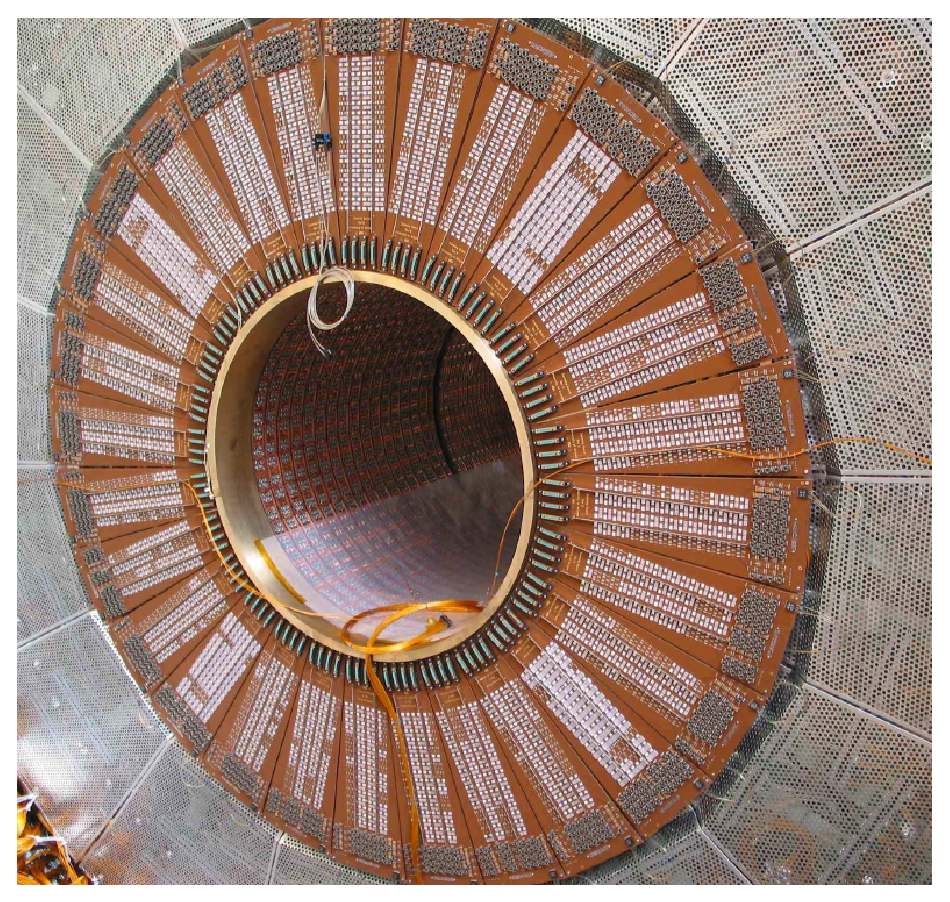
\includegraphics[width=0.8\linewidth,angle=0]{TBoverview/summingboards.eps}
\end{center}
\caption[Summing boards for the FCal.]{The FCal summing boards mounted on the rear of the HEC\cite{FCal_jinst_2010}}
\label{fig_summing_board_hec}
\end{figure}
%In \atlas, the signal from is read out from the end plate closest to the interaction point, whereas signals from FCal2 and FCal3 are read out from the end plate furthest from the interaction point. The shower maximum tends to be located between FCal1 and FCal2, and so the readouts are arranged in this way to minimise exposure of the electronics to radiation. 
\begin{figure}[tb]
\begin{center}
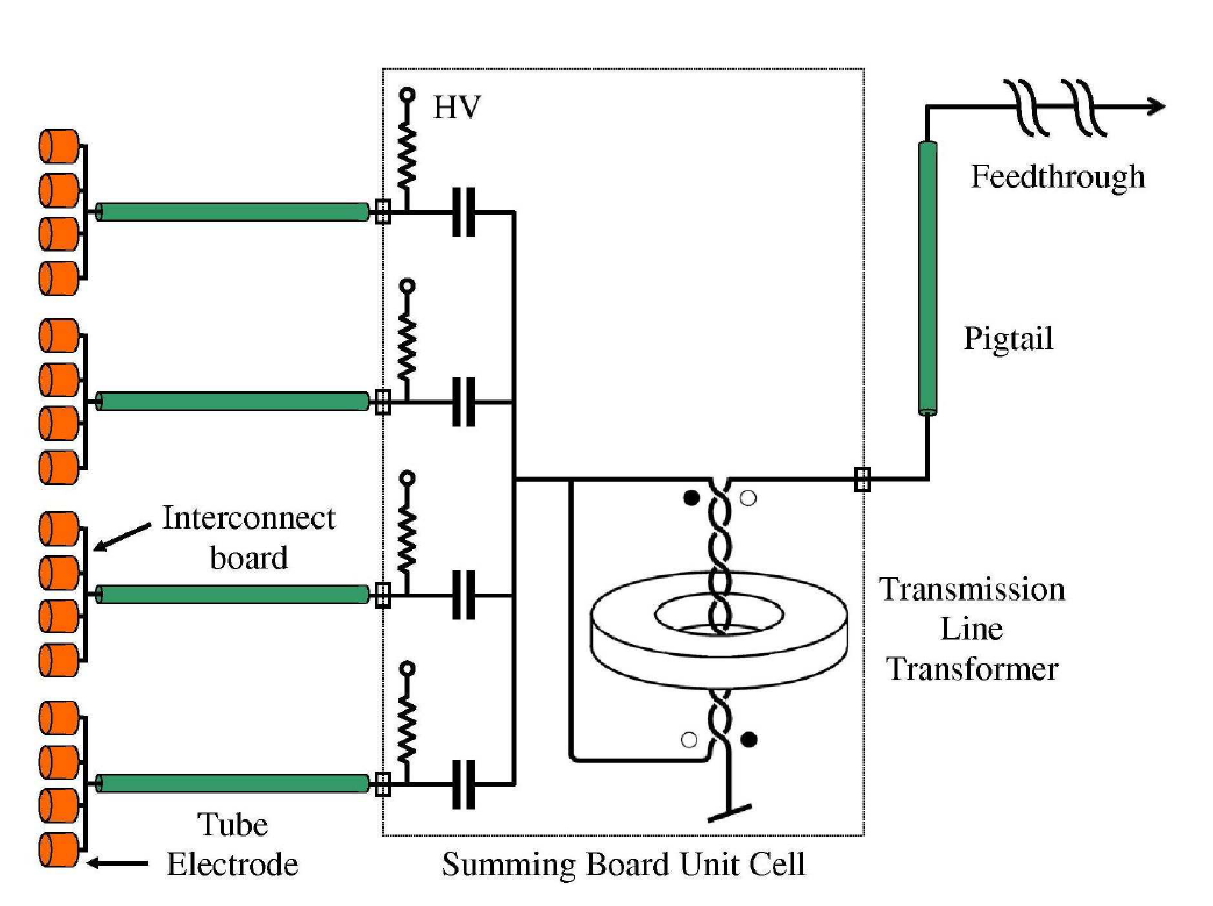
\includegraphics[width=0.8\linewidth,angle=0]{TBoverview/summing_board.eps}
\end{center}
\caption[Readout chain for a single summed FCal channel.]{Diagram of the FCal readout chain for a single summed channel. Summed channels are composed of four tube groups, which each consist of 4/6/9 electrodes in FCal1/FCal2/FCal3.}
\label{fig_sum_board}
\end{figure}

The readout lines are then fed out to summing boards, which are located on the rear of the HEC (i.e. inside the end-cap cryostats) as shown in Figure~\ref{fig_summing_board_hec}. On each summing board, signals from four interconnect boards are further combined to form a single readout channel. A typical FCal channel thus corresponds to four tube groups, which is equivalent to 16/24/36 electrodes in FCal1/FCal2/FCal3. The summing is carried out through a transmission line transformer, which serves to match the impedance of the readout coax to that of the ``pigtail'' cable used to carry the signal away from the summing board (Figure~\ref{fig_sum_board}). A different HV source is used to supply each tube group in a given channel, so that if one source fails then the other three tube groups in the channel should still be powered. This has occurred in \atlas: one of the lines supplying HV to the A-side FCal was severed during installation. This line supplies HV to one quadrant of FCal3, leaving one quarter of the tube groups in the affected area without HV. The remaining tube groups still contribute signal to the channels in this area, and so the effect of the severed HV line is corrected for during reconstruction.

Near the inner and outer edges of the FCal the tube groups are irregularly shaped. It is not practical to sum these channels in a coherent manner, and these ``unsummed'' channels also provide better readout granularity at high $|\eta|$.  
%The unsummed channels located near the inner edge (high $\eta$) also provide a readout with finer $\eta-\phi$ granularity than summed channels would in this region.

%\red{febs used by all LAr electronics?}

``Pigtail'' cables are  used to carry the signal from the summing boards to the cryostat feedthrough. Outside the cryostat, a stripline cable is used to carry the signal from the feedthrough to the Front End Boards.

\subsubsection{Front End Boards}
\label{sec_FEB}
Front End Boards (FEBs)\cite{ATLAS_FEB_design} are used in the electronics chains of all liquid argon calorimeters. Much of the following discussion applies to the electronics associated with all of these calorimeters, however some of the details mentioned here are specific to the electronics chain of the FCal. \cmt{The FEBs used during the beam test were prototypes, and had a similar design to those currently being used in \atlas. }

On the FEB, the signal is amplified and then shaped. The shaping consists of one differentiation and two integration steps (CR-${\rm RC}^2$) resulting in a bipolar pulse shape. This is done in order to optimise the signal with respect to pileup and electronics noise\cite{TDR_LAR,ATLAS_FEB_design}. In the other LAr calorimeters it takes much longer for the triangular current pulse to drop from its peak value back to zero due to the larger gap size\footnote{This time is $\sim$400~ns in the EM barrel but only $\sim 60$ ns in FCal1~\cite{FCal_jinst_2010}}. In these cases the shaping also allows the signal to be read out much faster, as the relevant information can be obtained from the first $\sim 125$ ns of the shaped pulse. 
%shaped pulse can be read out in , can be read out much faster allows the EM barrel calorimeter it takes $\sim 400$ns for the current pulse to drop from its peak value back to zero. In this case, the shaping allows for the  \blue{and also to reduce the signal collection time. In the EM barrel, triangular pulse takes ~400ns to drop to zero. Charge present in the LAr is proportional to the height of this pulse, and so it is unnecessary to measure the entire pulse to obtain this information. Shaped pulse can be read out in ~100ns }. 
Three different gains (low, medium, and high) are used when amplifying the signal. The amplification used for high gain is about 10 times as much as that used for medium gain, which in turn is about 10 times higher than that used for low gain. Each shaping chip processes the signals from four channels. An additional output on this chip sums the four inputs and then shapes the result. This output is used in the formation of trigger towers, which are discussed in section~\ref{sec_triggers}.

Timing on the FEB is managed by a Trigger Timing Control (TTC) chip, which distributes clock pulses every  25ns. The signal (at each gain) is sampled at every 25ns, and stored (as an analog voltage) on a Switched Capacitor Array (SCA) circuit. The pulse shapes for the three FCal modules are illustrated in Figure~\ref{fig_pulsehape}, showing the times at which the signals are sampled. Each pulse consists of an initial positive lobe followed by a longer negative lobe, the start of which can be seen in the Figure. \cmt{Note that the first sample is taken before the pulse starts to rise}

\begin{figure}[tb]
\begin{center}
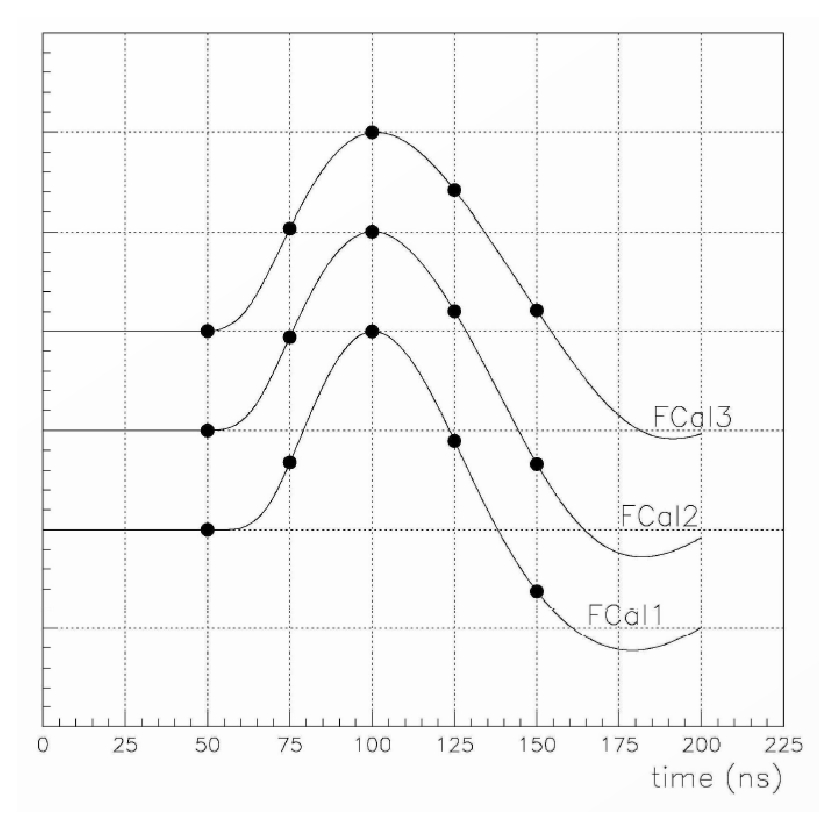
\includegraphics[width=0.6\linewidth,angle=0]{TBoverview/pulse_shapes.eps}
\end{center}
\caption[Pulse shapes for the FCal modules.]{Pulse shapes for each module. The dots indicate the times at which they are sampled and digitised.}
\label{fig_pulsehape}
\end{figure}

When a trigger signal indicates that an event should be read out, the pulse samples are read off the SCA and fed to an ADC (Analog to Digital Converter). For each sample the ADC then outputs a 12-bit signal\cmt{, which is a discretised voltage capable of taking one of 4,096 distinct levels}. Under normal operation only a single gain is read out of the SCA and digitised; a gain selector chip is used to determine which gain will yield the largest pulse height without saturating the ADC output. This is done by digitising a sample near the peak of the pulse at medium gain, and comparing the result to two pre-defined thresholds. If the value of the digitised sample lies between the thresholds then medium gain is used for the digitisation, otherwise low gain is used if the sample exceeds the upper threshold or high gain is used if the sample is smaller than the lower threshold.
%As the pulse shape has a negative lobe, a ``pedestal'' value must be subtracted from the digitised output in order to represent a negative value. 
In order to allow for negative values, e.g. samples taken on the negative lobe of the pulse, a ``pedestal'' value is subtracted from the digitised output. An offset voltage is added to the samples read from the SCA just prior to their digitisation~\cite{ATLAS_FEB_design}. This offset voltage is chosen such that the pedestal value is around 1,000 ADC counts, leaving around 3,000 ADC counts to represent the positive lobe of the pulse. For example, the negative lobe of a pulse may be sampled, and stored as a negative voltage in the SCA. Prior to digitisation, the sample is read from the SCA, and the offset voltage is added, such that the voltage to be digitised is positive. The digitised sample will then have a value of less than 1,000 ADC counts. When used to compute the channel energy (as discussed below), the pedestal value ($\sim$1,000 ADC counts) is first subtracted, such that the value associated with this sample is negative.

For the testbeam studies discussed in chapter~\ref{chapTB} the pedestal values were obtained from physics data on a run by run basis. For each channel, the first sample of each pulse was averaged over the entire run, and this value was used as the pedestal during reconstruction. Note that the first sample is taken before the pulse starts to rise, as illustrated in figure~\ref{fig_pulsehape}. In \atlas, the pedestal values for each channel are obtained from electronic calibration runs.


%The pedestal value During data taking the pedestal value was estimated \red{data taking pedestal monitored, reconstruction used average of first sample over a run.} 

%After shaping, the pulse has a bipolar shape. in order to obtain a pulse like that shown in figure~\ref{}.
%
%Febs used were prototypes, similar to final \atlas design
%trigger timing control TTC on FEB controls when data sampled/read out (every 25 ns)
%beam triggers not synched to this (unlike LHC)
%signal 

%The pulse is bipolar, prevents electronics being charged (?). Sampled at 25ns intervals, digitised. Pedestals. gains. 





%
% TTC every 25 ns.
%S1 random with respect to this, so LeCroy TDC used to measure time shift/phase between TTC and S1 with 50ps resolution. Second TDC used to remove phase ambiguity at 0/25 ns (are things exactly in time or 25ns off?) 
%
%because things arrive asynchronously, OFCs computed for 1ns bins of phase difference, i.e. 25 different sets of OFCs derived. timing phase used to select OFCs used for signal reconstruction.
%
%Pedestal - physics triggers, first (of seven) sample used for pedestal studies. Pedestal subtracted from pulse. 
%
%Pedestal value calculated for each channel, run by run. Noise for each sample taken as RMS of pedestal - 3.2 ADC on average.
%










%preamplified, converted to voltage, shaped (gains), sampled every 25 ns (held in pipeline), digitised by ADC (when L1 decides to read out). 
%
%Mention timing? don't mention timing
%
%summing boards inside cryostat (inner/outer walls of bathtub)




%transmission line transformer used to sum the signals from the readout cables and match them to the impedance of the "pigtail" coax. Pigtail has impedance of 25 ohm, in parallel the readout cables have an impedance of 6.25, so a 4:1 transformer is used. voltage of signal is doubled? no noise penalty - same noise as for one tube group.
%
%
%HV applied through resistors, so limit the current in case of a short.
%signals a.c. coupled through capacitors to 
%


\subsubsection{Signal Reconstruction/Optimal Filtering Method}
%\subsection{Optimal Filtering method}
\label{sec_signal_rec_OFC}
Offline reconstruction of the energy deposited in the calorimeter is done through the use of optimal filtering coefficients (OFCs)~\cite{OFC_paper}. These coefficients are used to reconstruct the amplitude of the signal pulse and its timing in such a way that the effect of the noise on the reconstruction is minimised. 
%
%For a signal pulse sampled at at regular intervals, the pulse height A and the time shift t may be found by forming the linear combinations

The OFC method produces two sets of coefficients, $a_i$ and $b_i$, which on average correctly produce the pulse amplitude $A$ and time shift $\tau$:
\begin{eqnarray}
A & = & \left \langle \sum_i a_i S_i  \right \rangle \label{eq_ofc_A} \\
A \tau & = & \left \langle \sum_i b_i S_i \right \rangle , \label{eq_ofc_AT}
\end{eqnarray}
where $S_i$ is the value of the $i$-th signal sample, after pedestal subtraction. Given that the pulse shape, $g(t)$  is known, these samples may be expressed as
\begin{equation}
\label{eq_OFC_taylor}
 S_i = A g(t_i - \tau) + n_i = A g(t_i) - A \tau g^\prime(t_i) +n_i, 
\end{equation}
where $g^\prime$ is the derivative of the pulse shape and $n_i$ is the noise present in the $i$-th sample. Equations \ref{eq_ofc_A} and \ref{eq_ofc_AT} may then be rewritten as 
 \begin{eqnarray}
A & = &  \sum_i a_i A g(t_i) -  a_i A \tau g^\prime(t_i)  + a_i \langle n_i \rangle  \label{eq_ofc_a2}\\
A \tau & = &  \sum_i b_i A g(t_i) -  b_i A \tau g^\prime(t_i)  + b_i \langle n_i \rangle \label{eq_ofc_at2}
\end{eqnarray}

The coefficients should be chosen in such a way that the variances of $A$ and $A \tau$ are minimised. As the mean value of the noise is zero, these variances may be written as
\begin{eqnarray}
{\rm Var} (A) = \sum_{i,j} a_i a_j \langle n_i n_j\rangle \\
{\rm Var} (A \tau) = \sum_{i,j} b_i b_j \langle n_i n_j\rangle ,
\end{eqnarray}
where $\langle n_i n_j \rangle$ is simply the autocorrelation matrix of the noise between samples. This minimisation may be carried out using the method of Lagrange multipliers, with constraints 
%\begin{eqnarray}
%
%
%\end{eqnarray}
\begin{displaymath}
\begin{array}{lll}
\sum_i a_i g_i = 1, & &\sum_i a_i g^\prime_i = 0\\
\sum_i b_i g_i = 0, & &\sum_i b_i g^\prime_i = -1
\end{array}
\end{displaymath}
obtained from equations~\ref{eq_ofc_a2} and \ref{eq_ofc_at2}.

For the testbeam studies discussed in chapter~\ref{chapTB}, a SPICE~\cite{SPICE_paper} simulation of the FCal electronics chain was used to obtain an initial estimate of the pulse shape used in the OFC calculation. This estimate was then improved using an iterative procedure that incorporated data taken from testbeam runs. The data used in this procedure are taken from events in which have a large pulse amplitude, in order to ensure that the signal is coming from a physical energy deposit. 
%In \atlas, the pulse shapes used to derive the OFCs for the EMB, EMEC and HEC are obtained using a method described below. For the FCal, 


%\clearpage


\subsubsection{Electronic Calibration}
\label{ECal}
After reconstructing the pulse amplitude, an ``ADC2MeV'' factor is applied in order to convert the pulse amplitude (in ADC counts) to the energy deposited in the calorimeter cell. For the FCal, the ADC2MeV value used during reconstruction is based on testbeam measurements (see section~\ref{TB_results_electrons}), and will be discussed further on page~\pageref{FCal_ecal_page}. For the other LAr calorimeters (EMB, EMEC and HEC), the ADC2MeV factor is obtained using an electronic calibration procedure. The ADC2MeV factor may be written as the following product:
\begin{equation}
F_{\mathrm{ADC}\rightarrow\mathrm{MeV}} = F_{\mu \mathrm{A}\rightarrow\mathrm{MeV}} \, F_{\mathrm{DAC}\rightarrow\mu\mathrm{A}} \, \frac{1}{M_\mathrm{phys}/M_\mathrm{calib}}  \, R.
\label{ECal_equation}
\end{equation}
%The factor $F_{\mu\mathrm{A}\rightarrow\mathrm{GeV}}$ describes the amount of energy that must be deposited in the calorimeter cell in order for the signal current in the calorimeter electrodes to have a peak value of 1 $\mu$A, while the factors R, FDAC and 1/M are derived from obtained from electronic calibration studies of the calorimeter, and will be discussed below.
The factors $F_{\mathrm{DAC}\rightarrow\mu\mathrm{A}}$, $R$, and $\frac{1}{M_\mathrm{phys}/M_\mathrm{calib}}$ are derived from electronic calibration studies of the calorimeter, and will be discussed below. The factor $F_{\mu\mathrm{A}\rightarrow\mathrm{MeV}}$ describes the amount of energy that must be deposited in the calorimeter cell in order for the signal current in the calorimeter electrodes to have a peak value of 1 $\mu$A. Note that $F_{\mu\mathrm{A}\rightarrow\mathrm{MeV}}$ is related to the sampling fraction, $f_\mathrm{samp}$, of the calorimeter, such that
\begin{equation}
\frac{1}{F_{\mu\mathrm{A}\rightarrow\mathrm{MeV}}} = \frac{f_\mathrm{samp}}{\tau_\mathrm{drift} E_\mathrm{ion}},
\end{equation}
where $E_\mathrm{ion}$ is the ionisation energy of argon (15.8 eV) and $\tau_\mathrm{drift}$ is the electron drift time in the calorimeter cell. 



All of the liquid argon calorimeters in \atlas make use of a calibration board, which injects a calibration pulse into the readout chain. In the FCal, this pulse is injected at the input to the FEB\cite{FCal_jinst_2010}, and so serves to monitor the electronic gain. In the EMEC, EM Barrel and HEC the pulse is injected at the calorimeter electrodes, and is also used to predict pulse shapes, channel by channel. 

Between LHC fills, electronic calibration studies of the LAr calorimeters may be performed. There are three types of calibration runs that may be undertaken during these studies: delay runs, ramp runs, and pedestal runs. Pedestal runs are used to record samples in the absence of any signal, and thus can be used to obtain the RMS of the electronics noise in the channel and the autocorrelation function of the noise. The noise autocorrelation function is used in the derivation of the OFCs, while the noise RMS is taken as the pedestal value, which is subtracted from pulse samples during reconstruction of the pulse peak.

 The calibration pulse is controlled by a 16-bit Digital-to-Analog Converter (DAC)\cite{LAr_Electronics}. In ramp runs, the amplitude of the injected calibration pulse is varied (``ramped''), and OFCs are then applied in order to reconstruct the pulse peak. This allows the relationship between the input current signal (in DAC) and the reconstructed pulse peak (in ADC) to be measured. A linear fit is performed to the (ADC,DAC) data, and the slope, $R$ (in units of DAC/ADC), is extracted. Thus, the factor of $R$ in equation~\ref{ECal_equation} functions as an ADC$\rightarrow$DAC conversion factor. The amplitude of the DAC signal and the peak value of the injected current pulse are related by the factor $F_{\mathrm{DAC}\rightarrow\mu\mathrm{A}}$, which depends on the specifics of the calibration board. The product $F_{\mathrm{DAC}\rightarrow\mu\mathrm{A}} \, R$ thus acts as an ADC$\rightarrow \mu$A conversion factor for calibration pulses.

%FCal CAL pulse goes into FEB input. other LAr calorimeters injected into calorimeter electrodes.
%
%For LAr electronics, a signal pulse resulting from ionisation has a triangular shape, whereas the calibration pulse may be described by a decaying exponential. 
%
%
%pulse delivered using DAC. Ramp runs get the R, which is 1/DAC->ADC. Delay runs mean that the shaped pulse may be measured. This gives DAC->muA. NO
%
%So, For a calibration pulse, the reconstructed pulse peak in ADC counts, A_{cal,ADC} and the amplitude of the injected current pulse in muA, A_inj, are related by
%
%A_inj = F_DAC_>mu_a \times R \times A_ADC.

However, signal pulses arising from ionisation have different shapes to the injected calibration pulses. Ionisation pulses are triangular, having a peak proportional to the number of ionisation electrons produced in the active region of the calorimeter cell and dropping to zero after the drift time has elapsed. The injected calibration pulses are shaped like decaying exponentials in order to approximate this triangular shape. This difference has an effect during the shaping. For example, in the case where an injected calibration pulse and an ionisation pulse both have the same initial peak current, the amplitude of the calibration pulse after shaping will be slightly lower than that of the ionisation pulse (as illustrated in Figure~\ref{fig_calibpulsehape}). 
\begin{figure}[tb]
\begin{center}
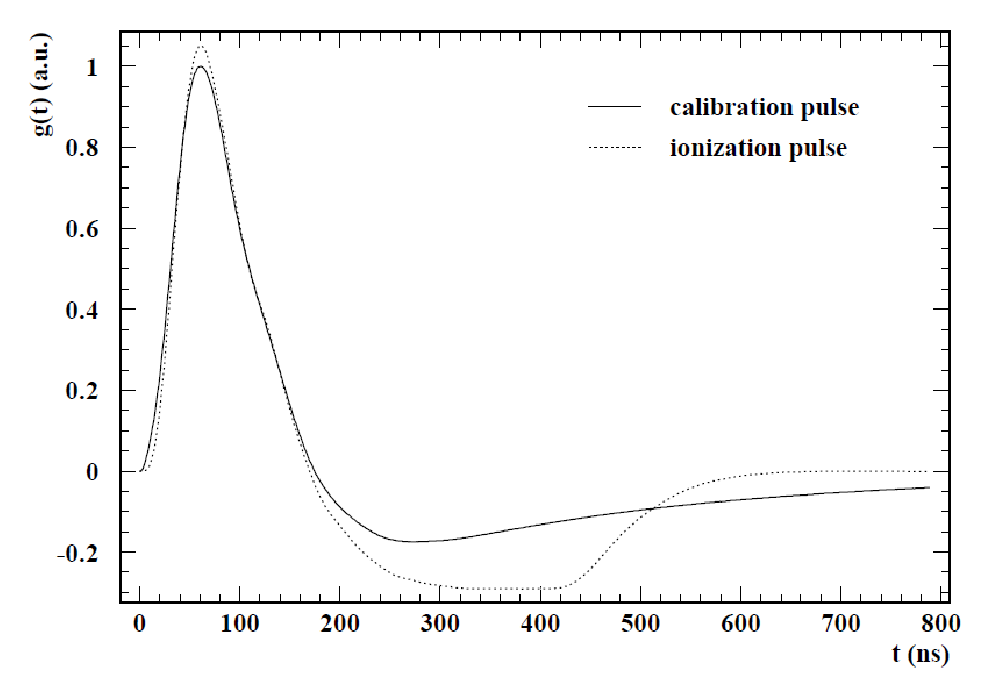
\includegraphics[width=0.6\linewidth,angle=0]{Detector/calibration_pulse_shape}
\end{center}
\caption[Calibration and ionisation pulses in the EMB.]{Calibration and ionisation pulse shapes for an EMB channel, after shaping. Prior to shaping, the peak current of the two pulses were equal~\cite{cell_equal}.}
\label{fig_calibpulsehape}
\end{figure}

Delay runs allow the pulse shapes to be measured. In delay runs, the calibration pulse is delayed (with respect to the TTC clock) by multiples of 1 ns. This effectively allows the shaped calibration pulse to be sampled at 1 ns intervals, which gives an accurate measurement of the shape of the calibration pulse. This information may then be used to infer the final shape of pulses originating from ionisation\cite{cell_equal}, which may then be used (together with the noise autocorrelation information obtained from pedestal runs) to derive the OFCs used for data taking at \atlas. The factor $M_\mathrm{phys}/M_\mathrm{calib}$ describes the ratio of the shaped ionisation pulse amplitude to that of the shaped calibration pulse amplitude, for cases in which both pulses have the same peak current prior to shaping. This factor corrects for the effect of pulse shaping, and thus allows the calibration factors (which are derived from calibration pulses) to be used for the calibration of ionisation pulses. 

For the FCal\label{FCal_ecal_page}, the calibration is based on testbeam studies rather than derived using calibration pulses. The factor $F_{\mu\mathrm{A}\rightarrow\mathrm{MeV}}$ may be calculated for each module from the geometry of the FCal electrodes and the other properties of the detector. The ADC2MeV value obtained from testbeam can then be used to derive a value of $F_{\mathrm{DAC} \rightarrow \mu\mathrm{A}}$ that is appropriate for the electronics used in \atlas. As the calibration is not derived from calibration pulses, the factor $\frac{1}{M_\mathrm{phys}/M_\mathrm{calib}}$ is not needed. Pedestal runs are used to measure noise in the electronics, but pulse shapes from testbeam data are used in the calculation of the OFCs (delay runs are not taken for the FCal). Ramp runs are still used to obtain $R$, and can thus be used to correct for any variations in the electronic gains.

%fuck you

%
% however the ramp runs are used to calculate the value of $R$.
%
% only pedestal runs and ramp runs are taken during electronic calibration.
%The OFCs are computed using the noise measured during pedestal runs with pulse shapes obtained from testbeam data. The factors 





  

%The factor 1/M/M corrects for this effect, thus allowing values of F derived from calibration pulses to be used to calibrate pulses caused by ionisation in the calorimeter. \red{mention that this requires knowledge of the ionisation pulse shape. But calibration data allows certain electrical properties of the readout chain to be measured, and analysis of the readout electronics then allows the shape of an ionisation pulse to be inferred from the (measured) calibration pulse shape.Cite cell response equal}
%
%So, for equation \ref{}, the factors R\times F_dac->muA equate to an ADC->muA factor appropriate for calibration pulses, while the M/M factor corrects this such that it may be used for ionisation pulses. Finally, the FmuA->GeV converts the electrode current into the ionisation energy deposited in the active region of the calorimeter, and scales this value by the sampling fraction of the calorimeter. 
%
%cite cell response equal, electronic_calibration, LAr_electronics
%
%%liquid argon electronics, electrode current is triangular peak so signal current is just charge deposited in active region via ionisation divided by the maximum electron drift time. the factor F may thus be obtained from geant4 simulations of the calorimeter, comparing the amount of energy deposited in the active regions via ionisation to the total amount of energy deposited in the calorimeter.
%%
%This factor must be determined from either 
%
%need an ADC2GEV factor.
%find this from calibration runs. 
%
%

%\clearpage


%
%
%TGCs
%
%RPCs
%
%
%
%
%toroidal magnets, barrel and two end-caps
%
%four systems Monitored Drift Tubes, Cathode Strip Chambers, Resistive Plate Chambers, Thin Gap Chambers
%
%TGC's and RPC's used for triggering, MDT's and CSC's used for measurement




\subsection{Trigger and Data Acquisition}
\label{sec_triggers}
%Do electron triggers work the same way as jet triggers?
%
%talk about jet triggers, or just triggers in general. Don't go into specifics about electrons and muons.
%
%% forward jet triggers - split in phi into two ``pseudo'' jet elements, then algorithm is run. Equivalent to requiring trigger tower to pass the threshold.
%
%at design, bunches cross every 25ns. need trigger to decide which events to write out.
%Three levels, L1, L2, and EF. L2 and EF make up the HLT. L1 is hardware, L2 is hardware/software.
%
%L1 has to make a decision within XX. 
%
%definitely need some data quality


%interactions occur at a rate of 40 MHZ. too often to record every event
%
%trigger used to determine which events are interesting and should thus be written out
%
%maximum accept rate at L1 is 75 kHz

\cmt{simple/complex deadtime?}

Collisions between proton bunches occur at \atlas at a design rate of 40 MHz, however, the maximum rate at which events can be recorded is limited by computing resources and is presently $\sim 400$ Hz\cmt{\footnote{The trigger system was originally designed to record events at $\sim 200$Hz, but is currently functioning at a much higher rate}}. The trigger system is designed to ensure that as many interesting events are recorded as possible, while rejecting less interesting events that occur at high rates, as shown in Figure~\ref{SMxsec}.\cmt{\red{could put the cross section plot of SM processes in here}} The \atlas trigger system consists of three consecutive levels: level one (L1), level 2 (L2), and the Event Filter (EF). The L1 trigger selects candidate events at a maximum rate of 75 kHz. Most of these events are subsequently rejected at L2, reducing the acceptance rate to 3.5 kHz. The final level of event rejection is done by the EF, which accepts events at the desired rate of $\sim 400$ Hz. 

%The L2 and EF together form the High Level Trigger, however until recently only the L1 trigger has been used for selecting forward jet events. 

The L1 trigger utilises custom-built hardware that is located off the detector, and needs to decide whether to accept or reject the event within 2.5 $\mu$s of the corresponding bunch crossing. While this decision is being made, information from detector channels is stored in pipeline memories, which are located on or near the detector.  The level 1 trigger consists of three of three parts, L1 Calo, L1 Muon, and the Central Trigger Processor (CTP). The L1 Calo trigger is used to select electrons, jets, taus, and other high \pt~ objects (excluding muons), while the L1 muon trigger processes signals from the RPCs and TGCs of the Muon Spectrometer. 

The CTP decides whether an event is accepted or rejected at L1. Trigger conditions are specified in a ``menu",  each item of which is some combination of trigger items from L1 Calo and/or L1 Muon. The CTP also handles the ``prescales'' on these menu items, which are used to control the bandwidth allowed for each item and keep the L1 acceptance rate at the desired level. For a menu item with a prescale of 50, one event will be accepted at L1 for every fifty events that satisfy the trigger conditions associated with that menu item. Menu items associated with a rare or particularly interesting event topology may be given a prescale of one, in which case the event is accepted every time the trigger conditions are met. Frequently occurring or less interesting topologies (such as those containing low-\pt~ jets) are given higher prescales.  
%
%
%
%%
%%Note that while the maximum rate at which events can be accepted at L1 is 75 kHz, during 2010 running this rate did not exceed 30kHz~\cite{trigger_2010}.
%%
%%things to add
%%detector data stored in buffers while waiting for L1A signal
%%L1A max latency of 2.5 us. nominally 2.1us. ``Large Fraction of this'' is in transmission time for signals to and from detector electronics.
%%L1 calo - custom electronics located off detector - decision made in less than 1us
%
%trigger towers - analogue sums 


The CTP also receives input from specialised detectors, such as ALFA (Absolute Luminosity For ATLAS), LUCID (Luminosity measurement using a Cherenkov Integrating Detector), the Beam Conditions Monitor (BCM) and the Minimum Bias Trigger Scintillators (MBTS). LUCID~\cite{LUCID} and ALFA~\cite{ALFA} are luminosity detectors located 17m and 240m from the \atlas interaction point, respectively, and were used to measure the luminosity delivered to \atlas during 2010. The BCM~\cite{BCM} is designed to monitor the condition of the beams and identify situations in which beams may be harmful to \atlas detectors (triggering a beam abort). It also provides a real time measurement of the luminosity at \atlas. The MBTS is used to select ``minimum bias'' events: the thresholds required to accept these events are very low, and so collision events are selected with minimal bias. These events are typically soft inelastic scatterings. The MBTS consists of tiles of scintillating polystyrene that are 2cm thick. There are 16 of these tiles mounted on the outer wall of each end-cap cryostat (on the side closest to the interaction point), covering the pseudorapidity range $2.09 < |\eta| < 3.84$. Early studies of the MBTS showed it to be very efficient, with an efficiency of over 99\% for selecting events in which there were at least 3 tracks with $\pt > 100$MeV~\cite{Tompkins_minbias}. Because of its high efficiency and low bias, the MBTS trigger was used as a reference when determining the efficiency of the jet triggers used in the inclusive jet and dijet cross section measurements, as discussed in section~\ref{incjet_triggers}. The distribution of charged particles obtained from minimum bias events recorded at \atlas is plotted in Figure~\ref{minbiasplot}~\cite{atlas_minbias}. Note that the distribution is roughly uniform in $\eta$. Due to the nonlinear relationship between $\eta$ and the polar angle, $\theta$, a fixed interval $\Delta \eta$ corresponds to a smaller angular interval at high $|\eta|$ than at low $|\eta|$. For example, one side of the EM Barrel has a length of 3.2 metres and covers the region $0<\eta<1.475$, while the FCal has an outer radius of $\sim450$mm and covers the region $3.2<\eta<4.9$: the FCal covers a larger pseudorapidity interval in a much smaller area. As the distribution of particles produced in minimum bias events varies slowly in $\eta$, detectors covering higher values of $\eta$ will be subject to a higher flux of particles than detectors located at low $\eta$. The effects of pile up are thus more significant for the FCal and end-cap calorimeters than for the barrel calorimeters.

\begin{figure}[tb]
\begin{center}
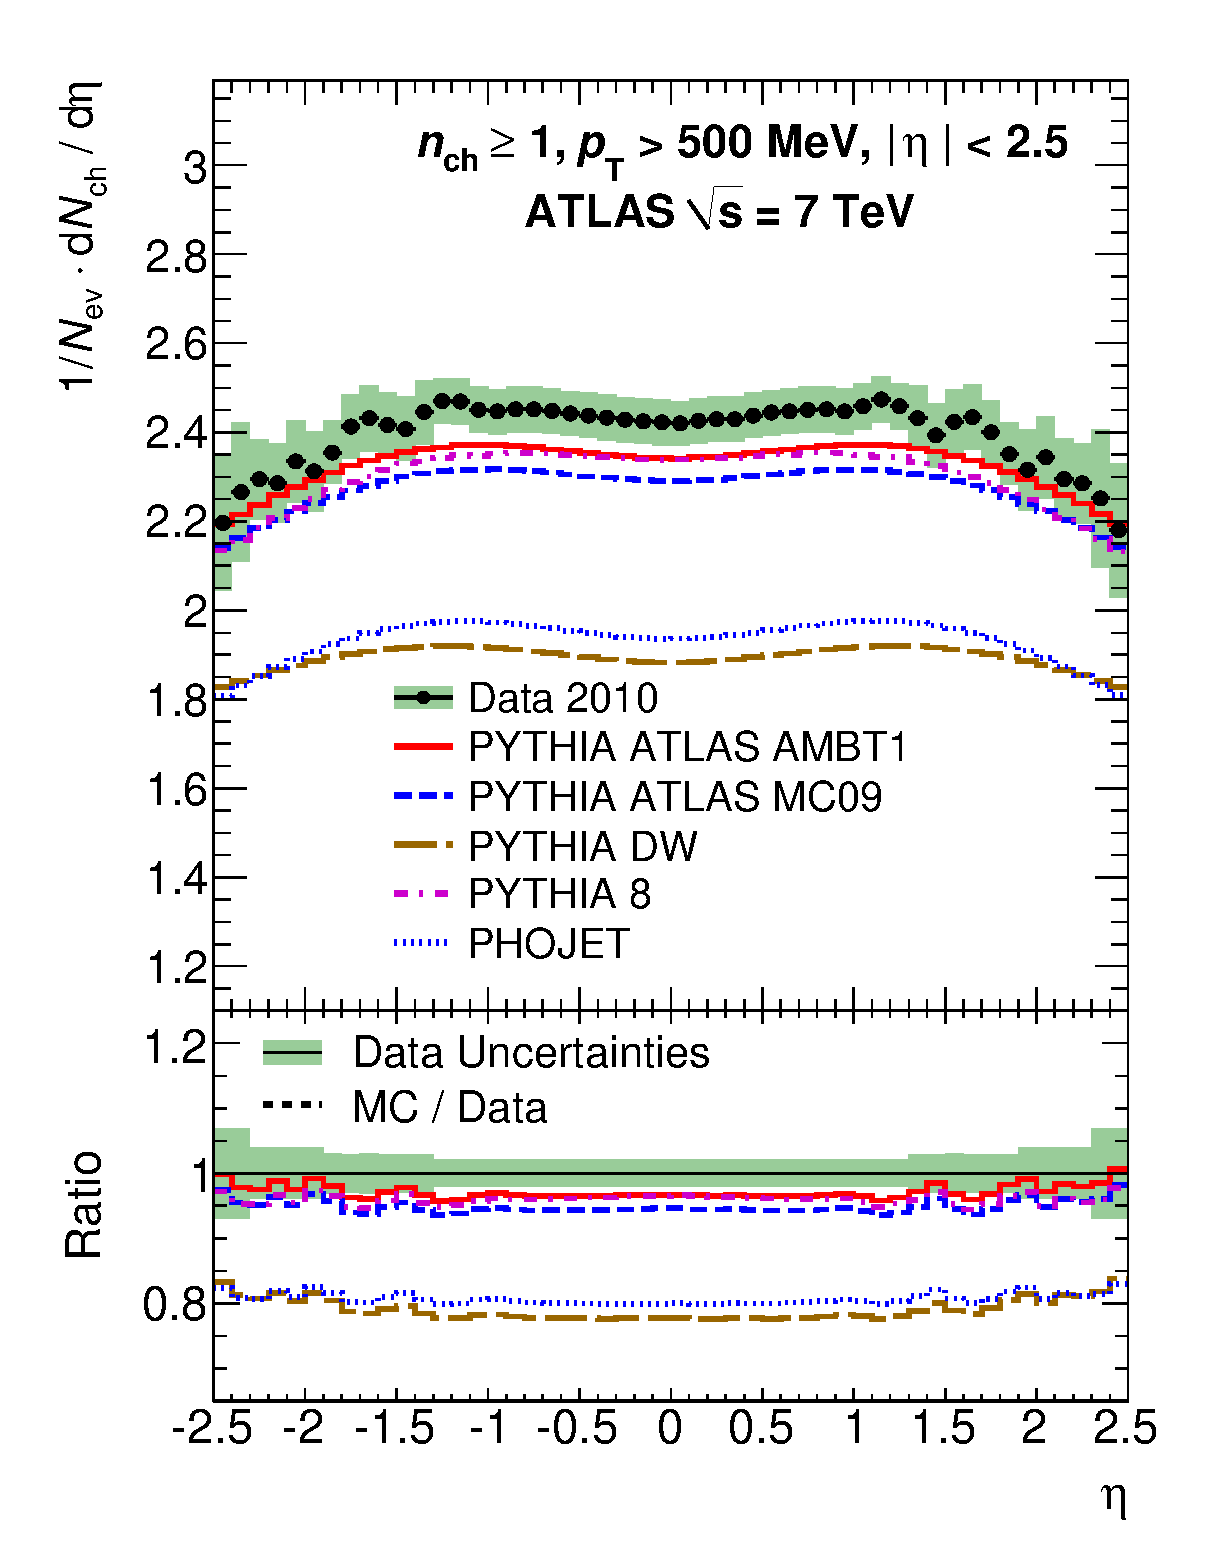
\includegraphics[width=0.6\linewidth,angle=0]{atlas_7tev_minbias.eps}
\end{center}
\caption[Distribution of charged particles in minimum-bias events.]{Distribution of charged particles produced in minimum bias events\cite{atlas_minbias}. The plot shows data measured at ATLAS, as well as predictions obtained from Monte Carlo simulations using a variety of tunes. Note that the plot only covers the region $-2.5 < \eta < 2.5$, as Inner Detector coverage is limited to this interval.}
\label{minbiasplot}
\end{figure}

The time available for the L1 decision is too short for L1 Calo to consider the information from individual calorimeter cells. Cell information is stored in the detector electronics, and only read out when an L1 accept signal is received from the CTP. Of the 2.5 $\mu$s available at L1, the decision is usually made within 2.1$\mu$s. However, a large fraction of this time is taken up by the transit time for signals to propagate between the trigger hardware and the detector, while L1 Calo processes events in less than 1 $\mu$s. Instead of relying on cell information, calorimeter signals are instead processed into ``trigger towers'', which are then sent as input to L1 Calo. Trigger towers are formed from analog sums of readout channel signals, as discussed in Section~\ref{sec_FEB}. In the Tile calorimeter, a trigger tower is formed by summing the signals from five channels. In the LAr calorimeters, the first two stages of summation are carried out on the FEBs, while the remaining addition is carried out on dedicated Tower Builder Boards (for the EMB and EMEC) or Tower Driver Boards (for the HEC and FCal)\cite{ATLAS_front_end_electronics}. In the barrel and end-cap regions $(|\eta| < 3.2)$, the trigger towers have a granularity 0.1$\times$0.1 in $\eta$ and $\phi$, whereas in the FCal the trigger towers have a granularity of approximately 0.4 $\times$ 0.4.

\subsubsection{Jet Triggers}

The level 1 central jet trigger combines 2$\times$2 blocks of trigger towers to form ``jet elements", which then have a granularity of  0.2$\times$0.2 in $\eta - \phi$ space. A sliding window algorithm\cite{ATLAS_L1Calo} is then used to identify jets. The window consists of a 4$\times$4 grid of jet elements, and a jet is identified if the total transverse energy within the window exceeds a given threshold. For example, the ``L1\_J10'' algorithm requires the transverse energy (at the EM scale) in the window to exceed 10 GeV. Additionally, the $2 \times 2$ cluster of jet elements in the centre of the window is required to be a local maximum; that is, the central cluster must have a transverse energy greater than that of any other $2\times2$ block of jet elements within the window.\cmt{ higher than any other cluster on two sides, equal or greater on other two}. If these criteria are met, then the event is accepted by the jet algorithm. The $0.4\times0.4$ area of $\eta-\phi$ at the centre of the window is then identified as a ``Region of Interest'' (ROI), and is passed on to any relevant L2 trigger algorithms. 

The forward jet trigger is used to identify jets in the region $|\eta| > 3.2$, and operates independently of the central jet trigger. While the central jet trigger uses information from the EM Barrel, Tile, EMEC and HEC calorimeters, only the forward jet trigger uses information from the FCal. Trigger towers in the FCal have a granularity of $\sim$0.4 $\times$ 0.4 in $\eta-\phi$, which is coarser than in other calorimeters. A jet element is then formed by summing all FCal trigger towers in $\eta$, such that the jet element has dimensions 1.6 $\times$ 0.4 in $\eta$ and $\phi$, respectively\cite{ATLAS_L1Calo}. Jets are then identified using the same sliding window algorithm that is used by the central jet trigger\cite{JEM_spec}.


At L2, the trigger decision needs to be made within 40ms. This interval is sufficient for cell-based methods to be used, although only cells within the region of interest (typically about 2\% of the detector) are read out. A cone-based algorithm is used for jet identification: a cone of fixed radius $\Delta R = \sqrt{\Delta \eta^2 + \Delta \phi^2}$ is positioned at the centre of the RoI. Energy weighted values of $\eta$ and $\phi$ are obtained by summing cells within the cone, and the centre of the cone is then moved to these coordinates. This process is carried out a predetermined number of times.

At the EF level, 4.0s of processing time is available, and so algorithms similar to those used for offline reconstruction (described in section~\ref{incjets_jetfinding}) may be used at the trigger level. Note that EF algorithms for jet triggers were not online while the data used in this thesis were being recorded, and so the trigger studies presented in section~\ref{incjet_triggers} focus on jet triggers at L1 and L2.



%At level 2

%The level 1 trigger is built on custom hardware utilising FPGAs, and needs to decide whether to accept or reject the event within 2.5 $\mu$s of the corresponding bunch crossing. 
%calo trigger

%L1 uses trigger towers. if accepted, identifies a RoI and passes this to L2. L2 looks at cells in the RoI, and has access to muon chambers and inner detector information. 
%
%Jet triggers blah blah. central Jet trigger covers uses up to eta < 3.2, while dedicated forward jet trigger uses information solely from the FCal. handy to use for triggering on events with forward jets, such VBF, where forward jets may be used to tag VBF event. 
%
%jet algorithms work like this at L1. Central trigger towers have this granularity.
%
%forward jet towers have this granularity, and so the L1 trigger does this.
%
%at L2 a cone algorithm is used.


%The level one trigger system is comprised of custom built hardware, and must decide whether to accept or reject an event within 2.5 $\mu s$ of the bunch crossing. This time interval is too short to look at detailed calorimeter cell information, and so the calorimeters are divided into trigger towers. In the central region, these have a granularity of 0.1$\times$0.1 in $\eta$ and $\phi$. The L1 jet trigger forms jet elements by summing 2$\times$2 blocks of trigger towers, thus giving an $\eta-\phi$ granularity of $0.2\times0.2$\cite{ATLASTrigger}. A sliding window algorithm is then run on the jet elements, and a jet is found if the transverse energy of a 2x2 cluster of elements from within the window passes a certain threshold. If so, the area is flagged as a region of interest and passed to the level two trigger. 
%
%Trigger towers in the FCal are more coarsely grained than in the central region, having a width of $0.4\times 0.4$ in $\eta-\phi$. Here the jet elements are formed by summing all towers in a phi slice, giving no granularity in $\eta$. 


%%\chapter{The ATLAS Detector}
%%\section{Inner Detector}
%%\section{Calorimeters}
%%\subsection{FCal?}
%%\section{Muon Spectrometer}
%
%%20 pages
%
%\chapter{The Standard Model/QCD}
%%15-20 pages
%\chapter{Calorimetry?}
%%%%10-15 pages
%%5-10
%



%testbeams - module 0 1998


%TODO:
%
%
%
% 
%%pulse figure - lots of figures

% references

% FLOWCHART.


%HV - one quadrant of FCal 3A  (upper left if looking from IP?)



\chapter{TestBeam Overview}
\label{chap_TB_intro}
\section{Introduction}

%\red{ test test} this should reference the CT10 fig \cite{CT10fig}.


%\red{intro to Testbeam studies here. 95, 98, 2000?, 2004, etc.}

%93 BNL - short depth EM module prototype -proof of principal, basic performance parameters
%95 CERN - full depth EM prototype - full depth - EM response
%98 CERN - FCAL1 and FCAL2 full depth module 0 prototype. - ratio of FCAL1/FCAL2 response/SF
%full depth 1/4 segments
%2003 - actual ATLAS FCAL C side
%2004 - ctb - uses module 0's from 1998

\red{purpose of TB}

The first testbeam studies of the ATLAS Forward Calorimeter were carried out in 1993, using an early prototype of the FCal1 module\cite{TB93_prototype}. This study provided proof of principle of the calorimeter design, and based on the results the design was adopted by the ATLAS collaboration \cite{TB93_prototype}. The prototype used in these studies was made of brass instead of copper and had a depth of 25cm, which is approximately half the depth of the FCal1 module presently being used in ATLAS. A subsequent beam test was carried out in 1995 using a full-depth FCal1 prototype \cite{TB95_prototype}. In 1998 further beam tests were carried out at CERN using full-depth ``module 0'' prototypes of FCal1 and FCal2, which allowed the response of the hadronic modules to be investigated for the first time \cite{TB98_testbeam_results,TB98_electron_signals}. The 2003 testbeam utilised all three of the C-side FCal modules presently operating in ATLAS, and will be discussed in detail in the following chapters. Following this, a 2004 combined testbeam studied the behaviour of the end cap calorimeters\cite{TB2004pub}. This included the refurbished ``module 0'' FCal1 and FCal2 prototypes used in the 1998 testbeam, as well as modules from the EMEC testbeam and purpose-built HEC modules.
%
%\red{add citations}
%
%% studies investigated the response of the module to electrons, using beam energies between 2 and 200 GeV. The results of these studies provided proof of principle 

The 2003 testbeam studies were carried out in the H6 beamline at CERN, which is fed by the Super Proton Synchrotron (SPS). Protons from the SPS were directed at fixed targets in order to produce secondary beams of the desired particles (electrons/positrons or charged pions) at the required energy.  

\begin{figure}[tbh]
\begin{center}
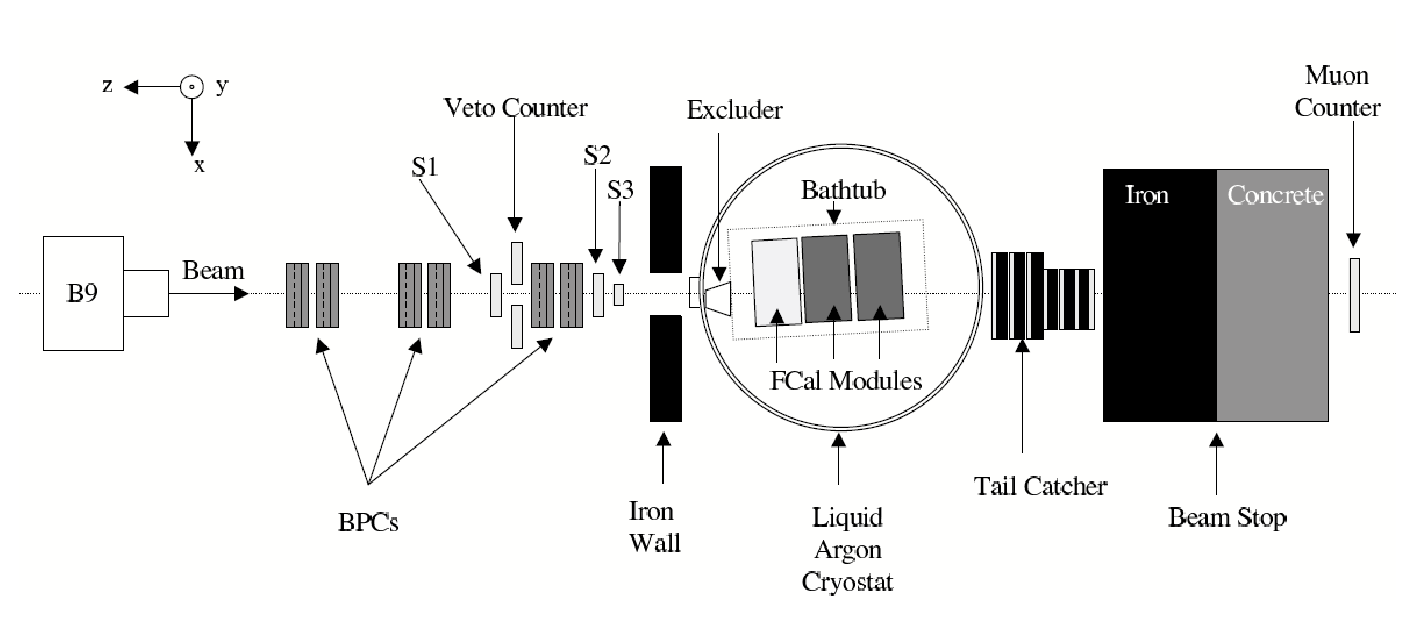
\includegraphics[width=0.8\linewidth,angle=0]{TB_Beamline}
\end{center}
%\centerline{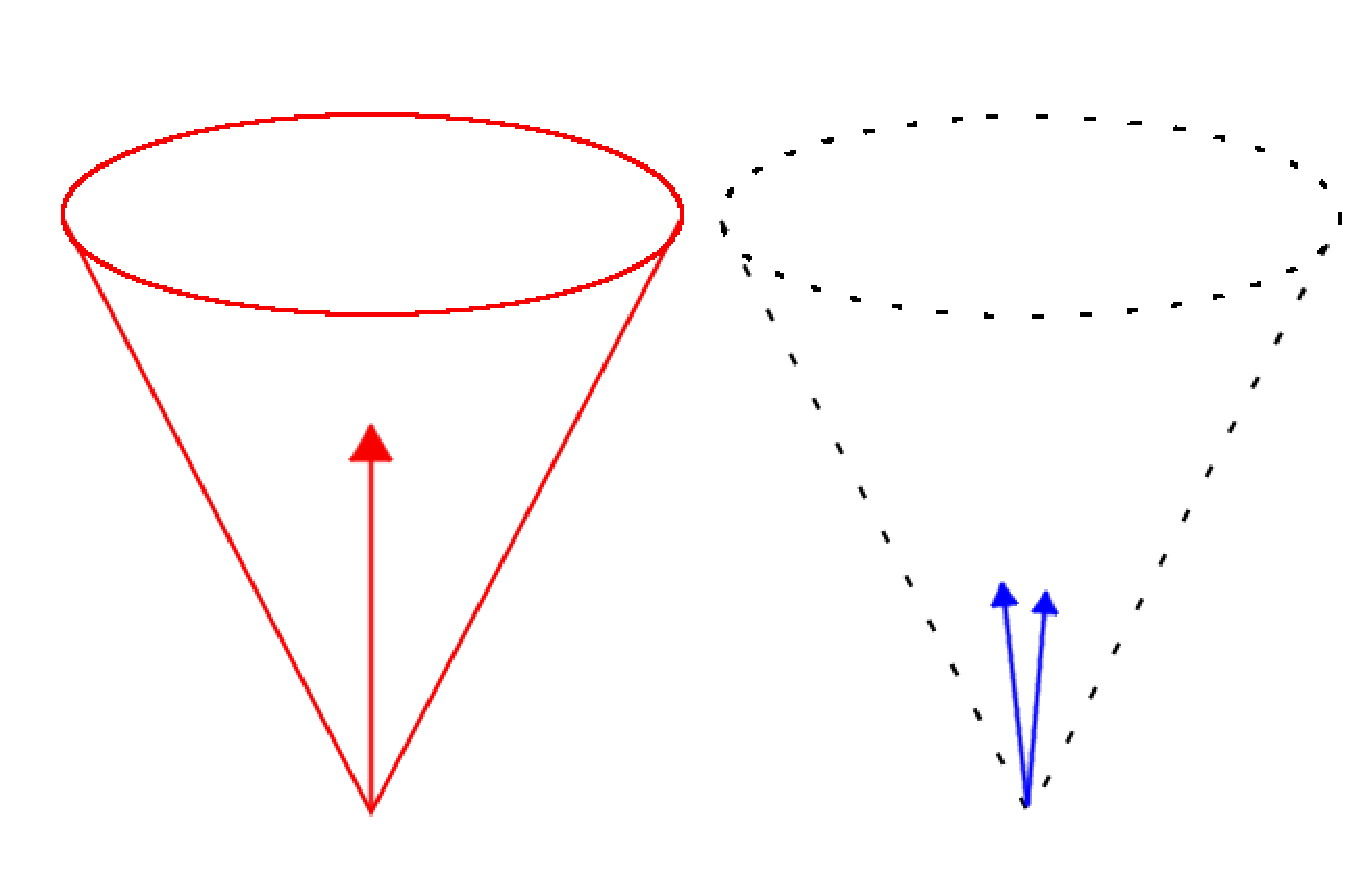
\epsfig{file=./figs/collinear.eps  , width=0.95\textwidth}}
\caption{Diagram showing the setup used for the 2003 FCal beam test (not to scale).}
\label{fig_TB_beamline}
\end{figure}

\begin{figure}[htb]
\begin{center}
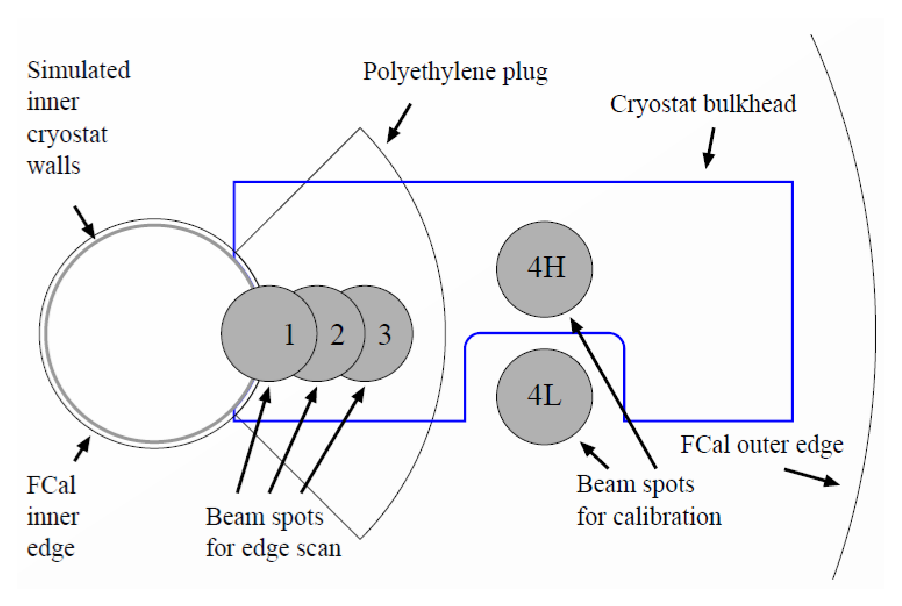
\includegraphics[width=0.8\linewidth,angle=0]{TB_beamspots}
\end{center}
%\centerline{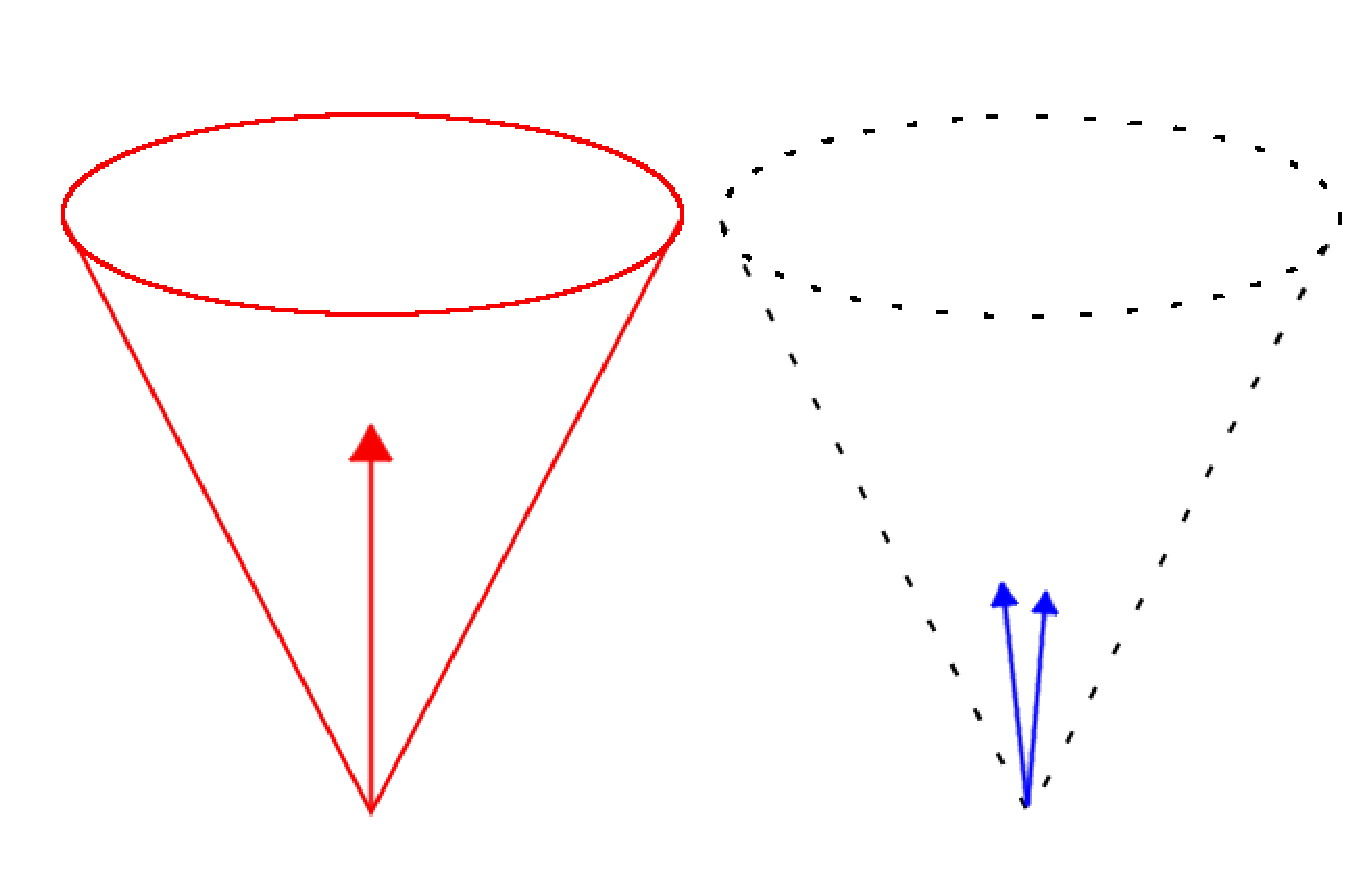
\epsfig{file=./figs/collinear.eps  , width=0.95\textwidth}}
\caption{Beamspots studied in the testbeam.}
\label{fig_TB_beamspots}
\end{figure}

A diagram of the beamline is shown in figure~\ref{fig_TB_beamline}. Beam particles emerge from the B9 magnet, traveling a distance of 32 metres and passing through several sets of instruments before reaching the FCal. The B9 magnet was used to control the vertical inclination of the beam, and thus the vertical position of the beamspot on the FCal face could be controlled via manipulation of the currents in the B9 magnet. The cryostat containing the FCal was able to be translated horizontally and rotated, which provided control over the horizontal position of the beamspot and the angle at which the beam particles struck the front face of the calorimeter. A total of 5 beamspots were used, numbered 1,2,3, 4L and 4H. The locations of these beamspots are depicted in figure~\ref{fig_TB_beamspots}. Positions 1,2 and 3 were used to study the effects of energy leakage down the beampipe from particles impacting close to the inner diameter. High energy ($\sim$200 GeV) beams of electrons and pions were used to provide data at these positions, and the results of these studies can be found in \cite{LouiseThesis,TB03_tbp}. Position 4L was used to study the intrinsic response of the FCal with a minimal amount of material between the calorimeter and the incoming particles, whereas position 4H was used to simulate a more \atlas-like environment with additional dead material introduced into the beamline. Electrons and pions at energies from 10-200GeV were used at these beamspots. This thesis will focus on the analysis of data taken at positions 4L and 4H, and the comparison of this data to results obtained from Monte Carlo simulations.
 



\section{Beamline Instrumentation}
%beam instrumentation and upstream material 
\label{sec_TBoverview_beamline}
\cmt{bpcs: positioning or profile? positioning in FCal paper}
Eight beam positioning chambers (BPCs) were used to provide tracking information on beam particles.
Four of these BPCs were of a more sophisticated design, one pair of which was located about 1.6 metres downstream from the B9 magnet while the other pair was situated 3m upstream from the FCal, on an adjustable table described below. These chambers each contain two readout planes, oriented at right angles such that measurements of both transverse coordinates may be made. Each readout plane covers an area of $120mm \times 120mm$, and has an average resolution of around $130 \mu m$. The other four BPCs were of an older design and were able to measure a single track coordinate with a resolution of about $325 \mu m$. These were positioned in the middle of the beamline (about 20m from the FCal), with two BPCs measuring the X coordinate of the beam particles and the other two the Y coordinate. In total, the eight BPCs provide six independent measurements of the X and Y coordinates of the beam particle tracks.

%\red{should talk about alignment here, or in results}
A mapping between BPC and calorimeter coordinates was established through analysis of electron data. The track measured by the BPCs was projected on to the calorimeter in order to obtain the beam impact point in the BPC coordinate system. This was then associated with the barycentre of the energy deposited in FCal1 using the calorimeter coordinate system. However, the finite granularity of the calorimeter readout tended to bias the position of the energy barycentres towards the centre of the readout cells. This was corrected for by considering the ratio $E_\mathrm{max}/E_1$, where $E_1$ was the total energy deposited in FCal1 and $E_\mathrm{max}$ was the largest energy value contained in a single channel. This ratio was plotted as a function of (BPC) $x$ and $y$, with minimal values in the ratio corresponding to cases where energy was shared evenly between multiple channels. The positions of the minima could thus be associated with cell boundaries in the calorimeter coordinate system, which then allowed the mapping between BPC and calorimeter coordinate systems to be determined with greater precision.
%
%
%Emax - max channel energy
%E1 - total FCal1 energy
%scan accross cell boundaries. 



The adjustable table was positioned about 2 metres upstream from the cryostat, on which three scintillators (S1, S2, S3) were positioned. These scintillators were polystyrene-based, and were used for triggering and ``beam cleaning'', which is discussed in section~\ref{sec_event_selection}. All three scintillators were 1 cm thick, with S1 and S2 having cross-sectional dimensions of 10cm $\times$ 10cm, while S3 had dimensions 7cm $\times$ 7cm. A veto counter was also present on the table, consisting of rectangular piece of scintillator (63cm $\times$ 63cm $\times$ 5cm) with a circular hole 65mm in diameter that the beam passed through. The height of this table could be varied such that the beam instruments were in the appropriate position for the beamspot under study. 

As the liquid argon gaps in the FCal are much smaller than those used in typical liquid argon calorimeters, FCal channels are susceptible to shorts should any conductive debris find its way into the liquid argon. Because the cryostat was not a particularly clean environment, the FCal was housed inside a ``bathtub'' which sat inside the cryostat. The bathtub was made from stainless steel 1.5 mm thick, and had a rectangular shape. Holes were present on its sides to allow the liquid argon to flow in as the cryostat was filled, but these were covered with a fine mesh to keep any debris out. 

\begin{figure}[h]
\begin{center}
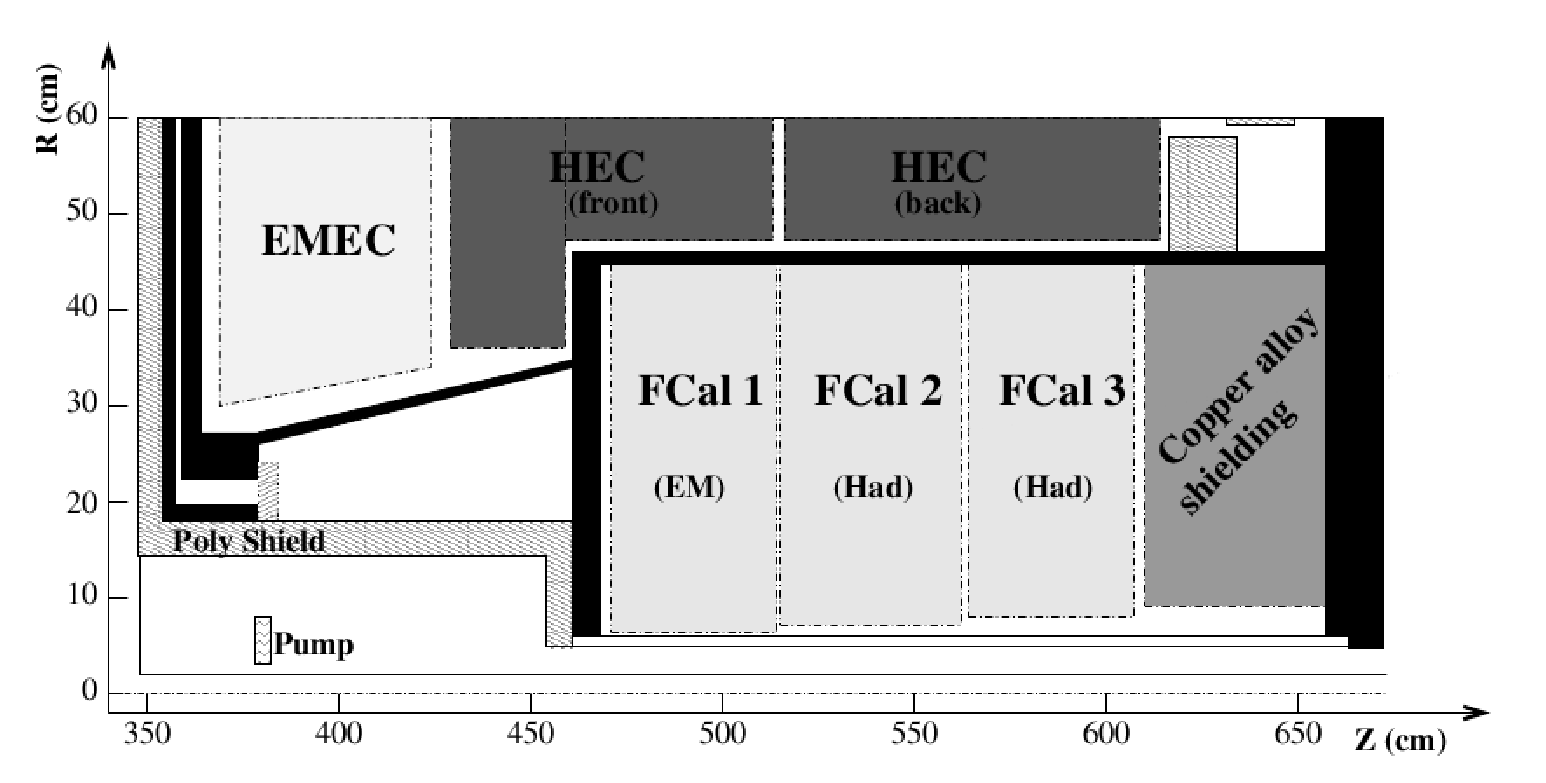
\includegraphics[width=0.8\linewidth,angle=0]{TBoverview/ECxsec_nolines.eps}
\end{center}

\caption{Cross section of FCal positioned within the end-cap cryostat, showing the inactive material laying between the calorimeter and the interaction point. The material in black is associated with the end-cap cryostat.}
\label{end_cap_xsec_2}
\end{figure}

In order to simulate a more \atlas-like environment for data taken at positions 1,2,3 and 4H, additional material was inserted into the beamline. A cross section of part of the \atlas end-cap is shown in figure~\ref{end_cap_xsec_2}, showing the uninstrumented (or ``dead'') material present in the end-cap. An aluminium plate 50.8mm thick was bolted to the inside of the bathtub to model the cryostat bulkhead, with a slot cut out of the plate such that the additional aluminium would not affect beams directed at position 4L. The area covered by this plate is shown in figure~\ref{fig_TB_beamspots}.

The JM shielding (labelled ``Poly Shield'' in figure~\ref{end_cap_xsec_2}) is made of boronated polyethylene and is present in \atlas to prevent albedo radiation from scattering back into the inner detector. This was modelled in the beam test by placing a wedge shaped piece of polyethylene on the outside of the bathtub such that it covered positions 1,2, and 3, simulating the toroidal ``plug'' part of the shielding that lies close to the beam pipe and adjacent to the cryostat bulkhead. An iron wall was located between the adjustable table and the cryostat. This wall had a 10cm x 10cm slot cut into it to allow the beam to pass through. When taking data at position 4H, a rectangularly shaped piece of polyethylene with dimensions 5cm x 20cm x 1m was placed at an angle in this slot. This was done in order to model the tube shaped part of the JM shielding that ran parrallel to the beam axis. When running at position 1, a small piece of aluminium was instead placed in this slot, simulating the ion pump present close to the beampipe in \atlas.

%An ``excluder'' made of RohaCell was also attached to the outside of the bathtub.
In \atlas, there is an evacuated area within the support tube, just in front of the FCal(as shown figure~\ref{}). The support tube used in \atlas was not present during the testbeam, and the FCal was instead mounted on a purpose-built stand within the cryostat. An ``excluder'' made of RohaCell was attached to the outside of the bathtub, in order to prevent the region of space correponding to the evacuated region in \atlas from being filled with liquid argon.
% In \atlas the area between the FCal support tube and the beampipe is evacuated, and so the excluder was placed inside the cryostat to prevent this space from being occupied by liquid argon.
 The density of RohaCell is 0.011 $\mathrm{g}/\mathrm{cm}^3$ whereas that of liquid argon is 1.43 $\mathrm{g}/\mathrm{cm}^3$, so the RohaCell provides a relatively good approximation of a vacuum. A hollow stainless steel cylinder was also placed inside the FCal during the beam test to simulate the beampipe.

A tail-catcher calorimeter comprised of layers of steel and scintillator was positioned downstream of the cryostat. Behind this was a beamstop of iron and concrete, and beyond that a muon counter was located. The tail-catcher and muon counter were only used for muon identification: energy deposited in the tail catcher is not considered when measuring the response of the FCal, or in the derivation of any weights presented in this analysis.

A CEDAR (Cherenkov Differential counter with Achromatic Ring focus, \cite{CEDAR_note}) detector was located upstream of the B9 magnet and used for particle identification. The CEDAR detector consisted of a chamber filled with gas (He) at high pressure. As beam particles passed through this chamber, they would emit Cherenkov radiation at an angle that depended on their velocity and mass. The optics of the CEDAR would then collect this light and focus it into a ring-shaped image, with different types of particles giving rings of different radii. An adjustable annular aperture was positioned in front of a series of photomultipliers, such that they would only detect light from rings of a given radius. The radius selected by the aperture could be tuned such that signal from the photomultipliers corresponded to a beam particle of the desired mass.

% As beam particles passed through a series of chambers filled with gas (He or $\mathrm{N}_2$) at high pressure, and emit Cherenkov radiation at an angle that is dependant on their velocity and mass. The optics of the detector then focus this into a ring, with different types of particles producing rings of differing radii. 

%
%
%
%
%
%
%
%
%\begin{figure}[h]
%\begin{center}
%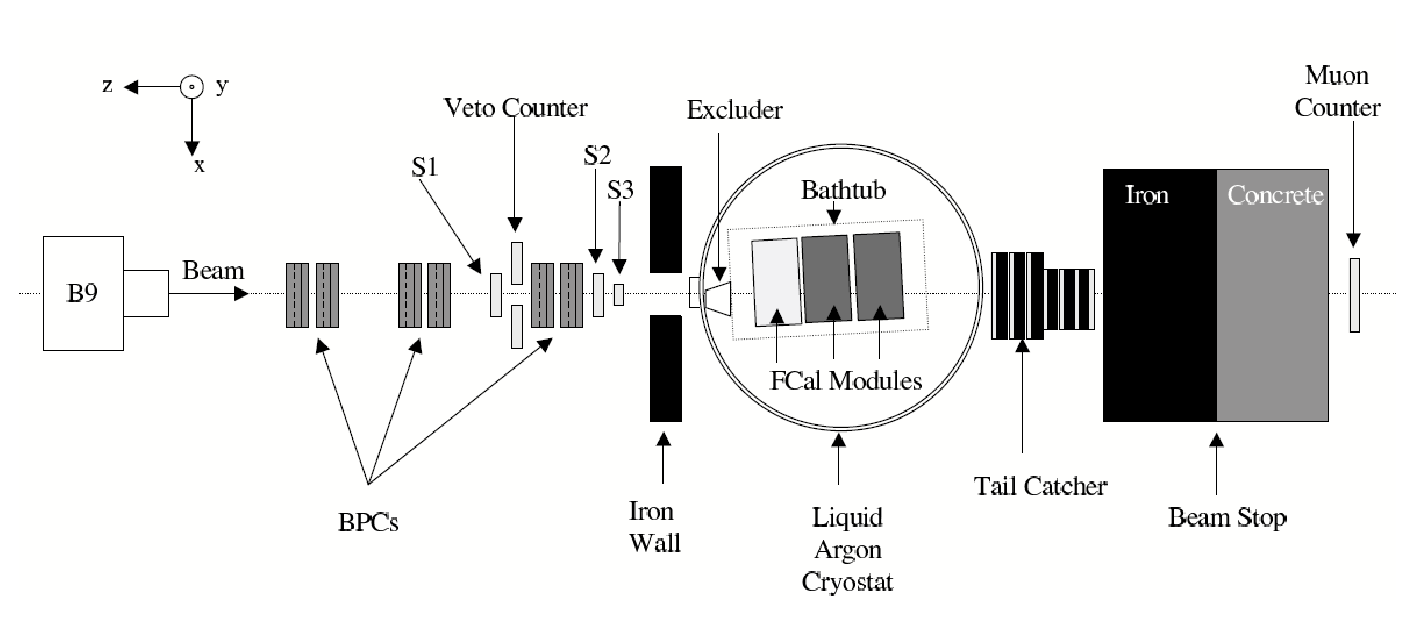
\includegraphics[width=0.8\linewidth,angle=0]{TB_Beamline}
%\end{center}
%%\centerline{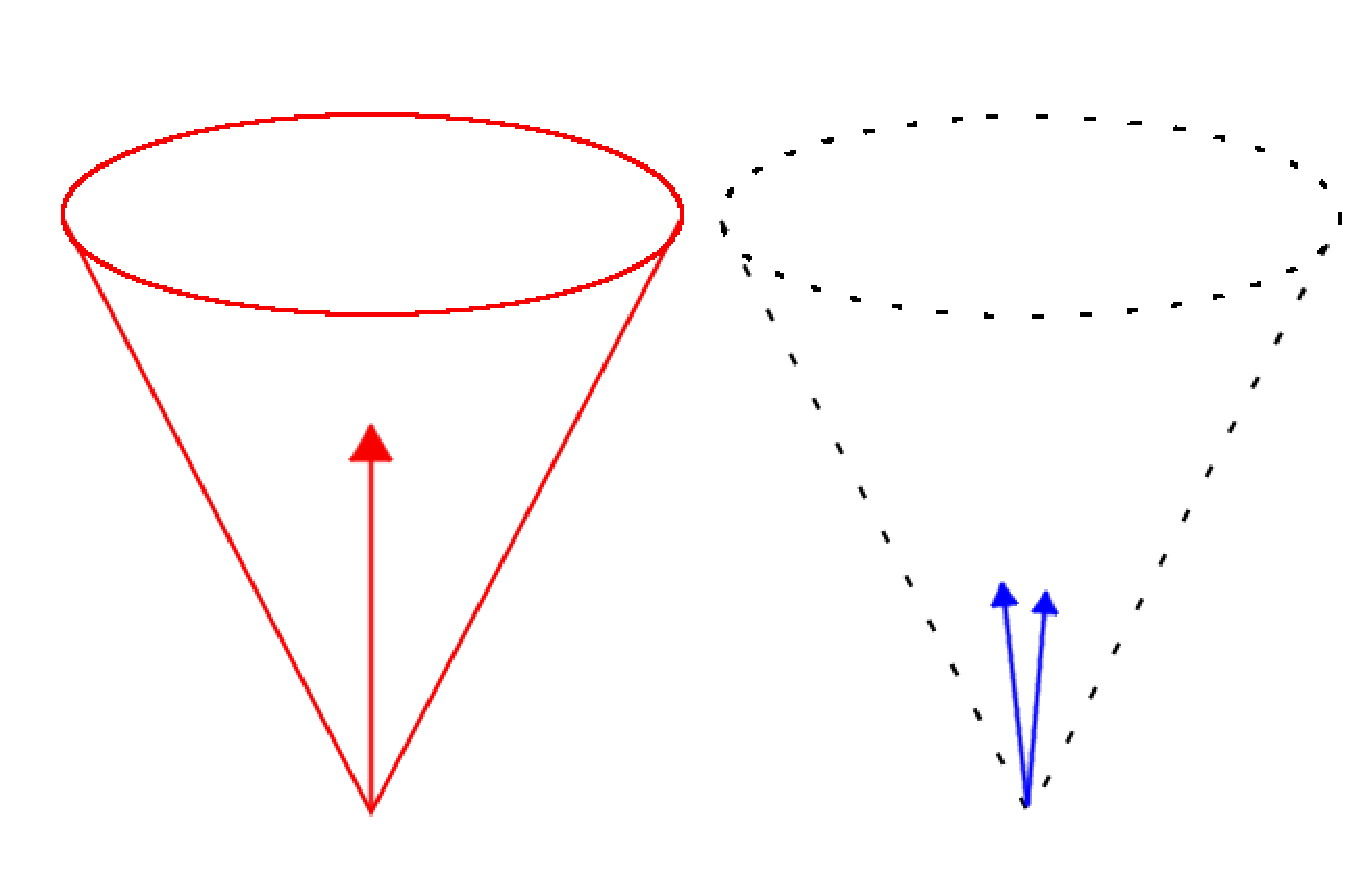
\epsfig{file=./figs/collinear.eps  , width=0.95\textwidth}}
%\caption{Diagram showing the setup used for the 2003 FCal beam test (not to scale).}
%\label{fig_TB_beamline}
%\end{figure}
%
%\begin{figure}[h]
%\begin{center}
%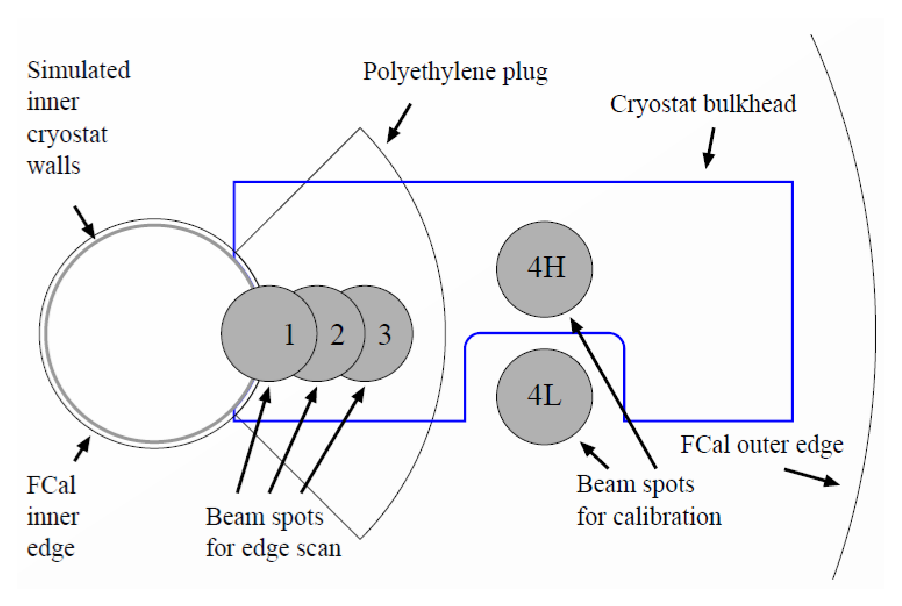
\includegraphics[width=0.8\linewidth,angle=0]{TB_beamspots}
%\end{center}
%%\centerline{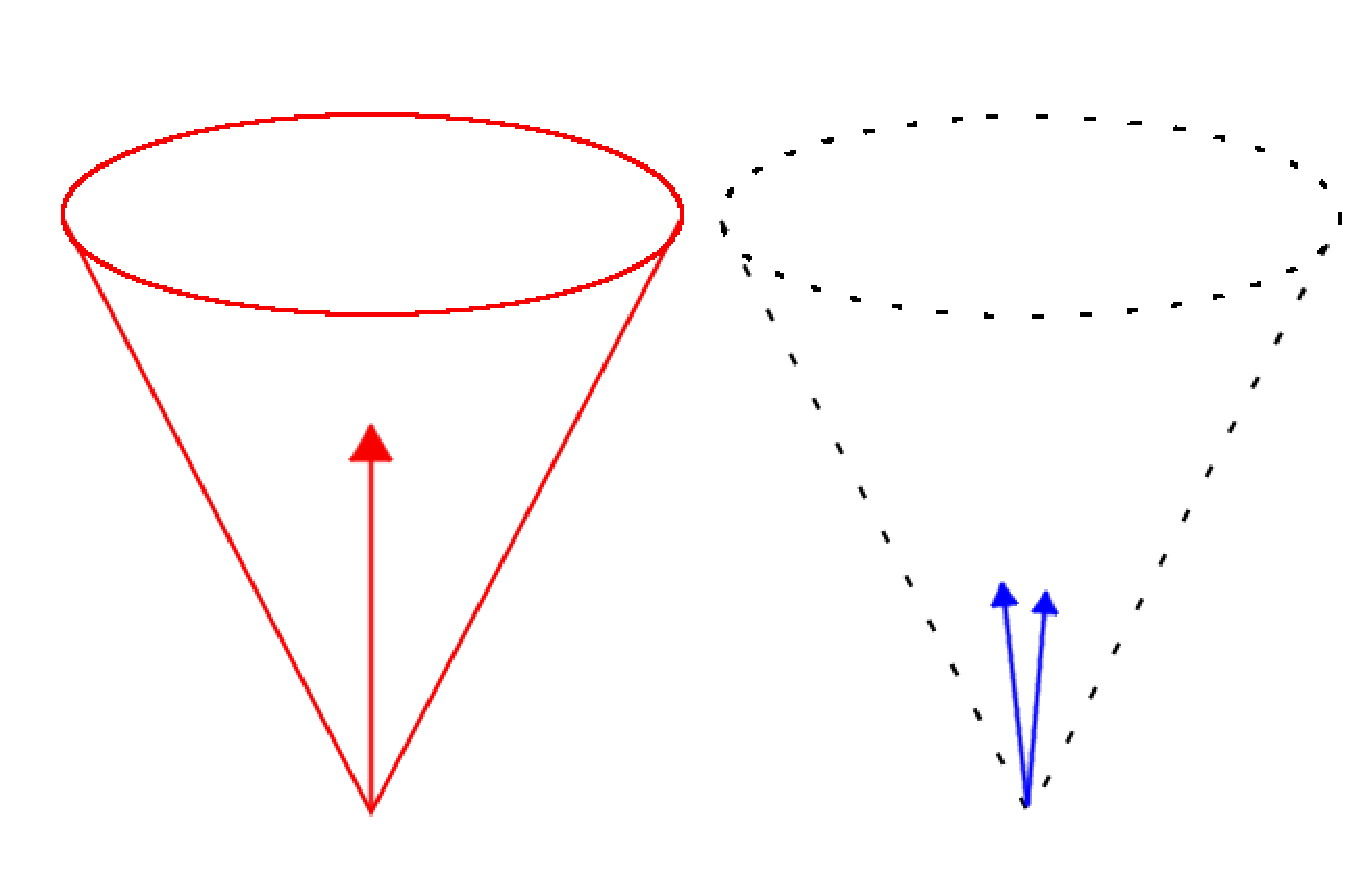
\epsfig{file=./figs/collinear.eps  , width=0.95\textwidth}}
%\caption{Beamspots studied in the testbeam.}
%\label{fig_TB_beamspots}
%\end{figure}
%
%


%
% 
%
% 
%
% Protons from the SPS beam were directed onto targets of in order to produce a secondadary/tertiary beam of the desired particle type.\red{(which targets for which particles?)} . \red{Then a magnet (velocity selector) was used to select particles of the desired type and energy}. 
%maybe skip the details here. secondary/tertiary beam emerges from B9, then stuff happens.
%
%
%
%
%This secondary beam of particles then passed through a bending magnet ("B9"), which controlled the vertical inclination of the beam. The vertical position of the beamspot on the FCal face could thus be manipuilated by varying the currents in the B9 magnet. 
%
%
%The cryostat containing the FCal was positioned 32 metres away from the B9 magnet. The 
%
%
%
%Six Beam Profile Chambers (BPCs) are used to obtain information on the trajectory of the beam particles. The 
%
%BPCs
%
%table scintillators, veto counter
%
%Iron wall, upstream material
%
%Cryostat
%aluminium plate, excluder
%bathtub
%FCal
%
%Tail Catcher
%
%
%\red{move FCal electronics and LAr signal reconstruction to Detector chapter. Keep Timing and offline reconstruction here.}



\subsection{Timing and Pulse Shapes}
\label{sec_TBoverview_timing}
%done using ofc method described in section~\ref{sec_signal_rec_OFC}.\cmt{\red{Test beam studies pulse shapes\ldots}} 
Reconstruction of the calorimeter signal was carried out using the OFC method described in section~\ref{sec_signal_rec_OFC} A SPICE \cite{SPICE_paper} simulation of the electronics chain was used to obtain an initial estimate of the pulse shape used in the OFC calculation. This estimate was then improved using an iterative procedure that incorporated data taken from physics runs. The data used in this procedure was taken from events in which the signal pulses had large amplitudes, in order to ensure that the signal was coming from a physical energy deposit.

Pulse shapes were sampled in time with the TTC clock on the FEBs (described in section~\ref{sec_FCal_electronics}). Seven samples were recorded for each pulse during physics runs, with the timing adjusted such that, on average, the fourth sample was coincident with the pulse peak. In \atlas the timing is synchronised to the LHC clock, such that samples are taken in time with each bunch crossing. This was not the case during the beam test, as beam particles arrived at random phases with respect to the TTC clock. In this case, timing for the event was taken from the S1 scintillator. A LeCroy 2228A Time to Digital Converter (TDC)  with a timing resolution of 50 ps was used to measure the phase difference between the event trigger and the TTC clock, with the trigger from the S1 scintillator used as a start signal and the clock pulse from the TTC used as a stop signal. The TDC only measured a phase difference between the start and stop signals, and so readings close to 0 or 25 ns were ambiguous. To resolve this a second TDC was used in which the stop signal was delayed by 10 ns, which allowed the time interval between the beam trigger and the TTC pulse to be determined uniquely. 

While the OFC method is capable of handling time differences between pulse peaks and sample times, the Taylor expansion used in equation \ref{eq_OFC_taylor} becomes invalid when this time, $\tau$, becomes large. To avoid this issue, events are binned according to the TDC phase time, using 25 bins of width 1 ns. A set of OFCS is calculated for each bin using a pulse shape that has been shifted in time by the relevant amount. During event reconstruction, the amplitude of each pulse is obtained by using the set of OFCs corresponding to the TDC phase time for that event. Only a single set of OFCs is required at \atlas, as in this case the TTC clocks are synchronised with that of the LHC, and so the samples are taken in time with the bunch crossings.

%
%For each of the 25 bins, a set of OFCs are calculated using a pulse shape shifted in time by the relevant amount. During signal reconstruction, the TDC phase time is used to look up the correct set
%
%
%
% 
%
%A SPICE simulation of the electronics chain is used to obtain an initial estimate of the pulse shape used in the OFC calculation. This estimate was then improved using an iterative procedure that incorporated data taken from physics runs. 
%
%To avoid this issue, 
%
%%The pulse shapes used in deriving the OFCs are taken from physics data, using events which had a large peak and were thus due to physical energy deposits.
%A SPICE simulation of the electronics chain is used to obtain an initial estimate of the pulse shape used in the OFC calculation. This estimate was then improved using an iterative procedure that incorporated data taken from physics runs.   
%
%
%The samples were fitted to a pulse shape prediction obtained through simulation of the electronics chain in order to find the time and amplitude of the pulse peak. Each pulse was then shifted and scaled so that the peak occured at time zero and had unit height. 
%
%
%
%
%
%
%OFC calculation.
%
%
%
%
%
% TTC every 25 ns.
%S1 random with respect to this, so LeCroy TDC used to measure time shift/phase between TTC and S1 with 50ps resolution. Second TDC used to remove phase ambiguity at 0/25 ns (are things exactly in time or 25ns off?) 
%
%because things arrive asynchronously, OFCs computed for 1ns bins of phase difference, i.e. 25 different sets of OFCs derived. timing phase used to select OFCs used for signal reconstruction.
%
%Pedestal - physics triggers, first (of seven) sample used for pedestal studies. Pedestal subtracted from pulse. 
%
%Pedestal value calculated for each channel, run by run. Noise for each sample taken as RMS of pedestal - 3.2 ADC on average.
%
%random trigger data used for noise autocorrelation?
%
%
%
%
%
%
%
%
%
%
%

\subsection{Offline Reconstruction}
\label{TBoverview_offline}
Offline reconstruction of testbeam data is carried out in \athena. A flowchart depicting the data structures and algorithms used in the reconstruction of data and simulation events is shown in Figure~\ref{TB_data_flowchart} For each event, the LArRawChannelBuilder algorithm retrieves the pulse samples (which are stored as LArDigits), and fetches the OFCs from a database. The pedestal is then subtracted from these samples and the OFCs are applied, giving the amplitude of the pulse in ADC counts. This amplitude is then converted to an energy using a factor (the ``ADC2MeV'' value) that depends on the channel and gain. The energy of the channel, in MeV, is then stored as a LArRawChannel object. Another algorithm is then used to create  CaloCell object from this LArRawChannel. From the CaloCell the position, time, energy, quality, and four-momentum of the channel may be retrieved, making CaloCells suitable objects to be used in data analysis. Because of this, CaloCell information is recorded by default in Event Summary Data (ESD) files, which are one of the standard formats used by \atlas. CaloCells are also used as input for topoclustering algorithms, which in turn are used as input for jet-finding and missing energy algorithms.

For initial studies of the testbeam data, the ADC2MeV factors used in the reconstruction were set to 1, so that the final energies were obtained in terms of ADC counts. This was done so that the actual ADC2MeV values could be extracted from the data more easily. However, the LArRawChannel class used in \athena stores channel energys as an integer number of MeV, as energies less than 1 MeV are deemed insignificant. An unforeseen consequence of this was that in earlier versions of the testbeam analysis, cell energies were truncated (rounded down) to an integer number of ADC counts. This rounding meant that energy was effectively lost during the reconstruction proccess, up to $\sim$80 MeV per cell in FCal1 and $\sim$160 ($\sim$185) MeV in FCal2 (FCal3). This had some effect on the electron results but a more significant effect on the hadron results, due to broader showers and higher ADC2MeV factors associated with the hadronic modules. The bug has since been fixed, and none of the results presented here are affected by it.


\begin{figure}[h]
\begin{center}
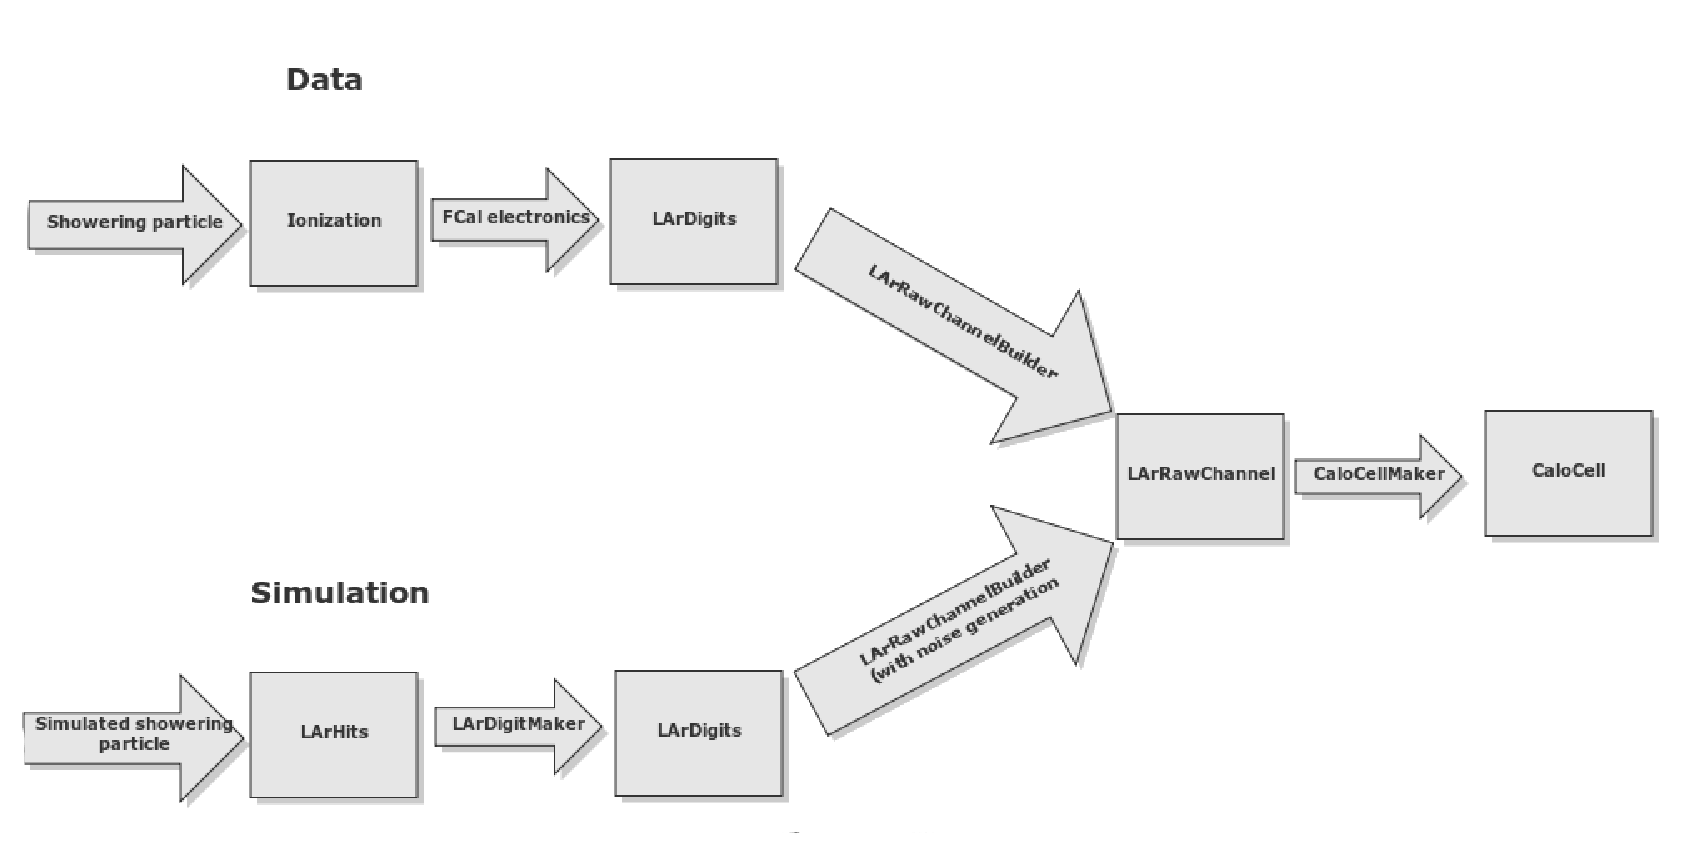
\includegraphics[width=0.9\linewidth,angle=0]{TBoverview/TB_data_flowchart.eps}
\end{center}

\caption{Flowchart showing the processes/algorithms and data structures involved in the reconstruction of testbeam data and simulation results.}
\label{TB_data_flowchart}
\end{figure}

\section{Monte Carlo Simulation}
%\subsection{Monte Carlo}
%\subsection{reconstruction}
%\subsection{noise}
%athena/G4/geometry
%digi/reco
%noise


A Monte Carlo simulation of the testbeam setup has been developed within the \athena framework. \cmt{The simulation describes all elements of the beamline from the B9 magnet to the tailcatcher.} Geant 4.9.2 \cite{geant4} is used to simulate interactions of the beam particles with beamline elements. The results of this simulation are then reconstructed and analyzed in the same manner as the data.

\subsection{Geant4 Simulation of the Forward Calorimeter and Testbeam Environment}
\label{TB_overview_g4}
Geometry in \geant is described in terms of volumes. A ``solid volume'' is first created to describe the shape of a given object. This is then used to derive a logical volume, which inherits the shape of the solid and is associated with a material. A material type is defined by specifying the relative mass fractions \cmt{of the elements of which it is composed} of its constituent elements and the density of the material. Logical volumes are then used to construct physical volumes \cmt{(PhysVols)}, which inherit the shape and material information from the logical volume. A physical volume also has a position and orientation assigned to it, and it is by positioning these physical volumes that the geometry of the simulation is defined. A special physical volume, the world volume, is created first. All subsequent physical volumes are then placed either inside the world, or inside another physical volume. 
%The position and orientation of a physical volume are specified through transformations: rotations and translations. A physical volume is placed at the origin of the volume it is inserted into, and transformation operations are then applied to reposition it. 

The description of the beamline used in the simulation contains all the beamline elements from the B9 magnet to the tailcatcher, including all scintillators, BPCs, cryostat material and beampipes. Most of these objects are defined from scratch, however the description of the FCal is taken from that used in the full \atlas simulation while the cryostat description has been taken from another testbeam simulation. Elements upstream of the B9 magnet, such as the CEDAR detector, have not been included. 

The description of the FCal has been modified in some respects, to improve some aspects of the material description. In the default FCal definition the rods in the hadronic modules are made of WFeNi whereas they are actually pure tungsten, which has a slightly higher density. The density of the absorber matrix was also corrected, as an updated estimate of this value was obtained. The correct materials and densities (given in section~\ref{chap_Detector_FCal}) have been used in the testbeam simulation.

%The abstract way in which positions are defined can also lead to errors. \geant uses matrices to represent transformations, and so the order of operations are important. When a physical volume is inserted into the world (or another physical volume), it is placed at the origin of that volume's coordinate system, and must be repositioned by applying transformations. These transformations are not commutative, so care must be taken to ensure the operations are applied in the correct order. The last operation specified prior to the creation of a physical volume is the first operation applied to it once it is placed in the world, which can be counterintuitive if these transformations are not thought of as matrix operations. 

%For example, the Cryostat description takes the z axis to be vertical, whereas in the geometry used by \atlas and the testbeam the z axis is the beamline (i.e. horizontal). The cryostat is thus rotated $90^\deg$ before being inserted into the world. Consequently, the 

In \geant, physics is defined in terms of processes. Particles are propagated through the simulation in a step by step fashion, with continuous processes (such as ionisation) acting on the particle during the step while discrete processes (such as decays, pair production) take place at the end of a step. After each step, the particle's kinematics are updated. Secondary particles are only produced if their energy exceeds a ``range cut''. If a process would produce a secondary particle with energy less than the range cut, this energy is instead deposited in the material. Range cuts are specified as a distance, but \geant converts this distance to an energy based on the material the particle is travelling through at the time. A range cut of $30 \mu m$ has been used for testbeam simulations, which is appropriate given the narrow width of the active liquid argon gaps. In the full \atlas simulation, range cuts of 100$\mu$m are used in the EM barrel and EMEC calorimeters, while a cut value of 1mm is used in the HEC. The full \atlas simulation also uses a range cut of $30 \mu m$ for the FCal.

%Interactions of particles with matter are done in a step by step manner. At each step, particles in the simulation are moved forward by an amount dependant on their kinematics and any physical processes that may be relevant.  
%
%http://geant4.web.cern.ch/geant4/UserDocumentation/UsersGuides/ForApplicationDeveloper/html/ch05.html#sect.Track
%
%Electromagnetic showers only consist of a relatively small number of  processes (e.g. Bremstrahlung, pair production, ionisation), and so are relatively straightforward to model.

Electromagnetic showers are generally well understood and relatively straightforward to model. Hadronic showers are more complex, and a variety of processes are used to describe the shower development. Hadronic ``physics lists'' are used to define the specific set of processses available and the energy ranges in which they are used. Three physics lists have been used in the simulation of the test beam, and are outlined below:

\begin{itemize}
\item{QGSP-BERT:} Quark Gluon String Precompound with Bertini cascade. This is the default physics list used for \atlas simulations. The Quark Gluon String model \cite{QGSP_paper} is used to simulate hard inelastic scattering for hadrons in with energies from 12 GeV to 100 TeV. One or more strings are formed between between partons of the colliding hadrons, and these strings are then ``cut'' by inserting quark/anti-quark pairs. One member of the pair becomes the new ``end'' of the string, while the other forms a hadron with the parton that was the old end. This process repeats until the string has insufficient energy to form new pairs. The precompound model is then used to de-excite what remains of the nucleus.
Between 9.5 and 25 GeV, a Low Energy Paramaterization (LEP) is used to describe inelastic scattering \cite{LEP_paper}. 
For particles with energy less than 10 GeV, a Bertini intra-nuclear cascade model \cite{ Bertini_paper, Bertini2} is used to describe inelastic scattering with nuclei. The incoming hadron is classically scattered within the nucleus, using cross sections and angular distributions taken from experiment. 
\item{QGSP-BERT-HP:} This physics list is essentially the same as QGSP\_BERT, but includes high precision modeling for low energy neutrons ( $<$20MeV). This method relies extensively on cross sections obtained from experiment. It was reported in \cite{QGSP_HP_note} that the high precision neutron tracking had a significant effect on the development of hadronic showers in tungsten, and so it was considered worthwhile to investigate this physics list.
\item{FTFP-BERT:} This physics list uses the Fritiof string model \cite{Fritiof_string_paper} to model high energy inelastic interactions, which is similar to the Quark-Gluon String model described above. The Fritiof model can be applied over a wide range of energies, and is used for hadrons with energies between 4 GeV and 100TeV. As with QGSP\_BERT, the precompound model is used to de-excite the nucleus following the Fritiof interaction. The Bertini Cascade model is also used at energies below 5 GeV.
\end{itemize}





%geometry - uses volumes. solid volumes for shape logical volumes for material/density,  physical for position within world.
%
%positioning carried out through transformations - translations and rotations. physical volumes placed within physical volumes.
%
%Some parts FCal, "based of descriptions used..."taken from \atlas or other simulations of beam tests of other detector components.
%need to be careful here. small errors were found in the densities and materials used in default \atlas simulation. For example, the rods used in the default simulation are made of WFeNi material rather than pure tungsten, which is of a slightly higher density. The density of the default absorber matrix was also found to be too high/low, whereas the correct value (14.39g/cm3, c.f. section XX) has been used in the testbeam simulation.
%
%Abstract way in which positions are defined can also lead to errors. Transformations (translations/rotations) are defined in terms of matrices, and the order of operations are important. When a physical volume is inserted into the world (or another physical volume), it is placed at the origin of that volume's coordinate system, and must be repositioned by applying transformations. These transformations are not commutative, so care must be taken to ensure the operations are applied in the correct order. The last operation specified prior to the creation of a physical volume is the first operation applied to it once it is placed in the world, which can be counterintuitive if these transformations are not thought of as matrix operations.
%
%The representation of the cryostat takes z direction as being vertical, whereas \atlas and the beam test use z to be the beamline. This kinda fucks everything up.
 
%Interactions of particles with matter (i.e. physical volumes) are carried out in a step by step fashion. 
%How does G4 work, exactly?
%
%kinematics ->get step size from processes
%move by the step
%update kinematics (all active processes used
%maybe decay?
%continue
%
%particles tracked untill they have no energy, but not produced unless they have enough energy to travel a certain distance, range cut.
%
%Electromagnetic showers pretty straightforward, consist of a few processes. Hadronic showers more complex, and various processes/models are used in the shower development. A Hadronic physics list is used to define the specific set of processes available and then energy ranges in which they may be used. Simulations have been run using the three physics lists described below
%
%QGSP\_BERT quark Gluon String Precompound with Bertini cascade QGString, fragments, interacts with precompund. Bertini used at lower energy
%
%FTFP\_BERT Fritiof string model, with bertini
%
%QGSP\_BERT\_HP. like QGSP\_BERT, but uses tables of data from neutron scattering. Investigated this physics list after it was noted in \cite{} that slow neutrons are important for showers in tungsten. generally gives results similar to QGSP\_BERT, but takes a lot longer to run.
%
%%http://geant4.cern.ch/support/proc_mod_catalog/physics_lists/hadronic/FTFP_BERT.html
%%http://geant4.cern.ch/support/proc_mod_catalog/physics_lists/hadronic/QGSP_BERT.html
%
%hits - showering particles deposit energy via ionisation in active region (LAr Gaps of FCal), information is stored as a G4 hit from which the energy, time, and location of the deposited energy can be accessed. A vector of these hits is stored for each FCal channel, and used as an input for the reconstruction. 
%%If desired, calibration hits can also be enabled, in which case information is stored for energy deposited in dead/inactive areas of the beamline, including the absorbing material of the calorimeters. This is useful for determing the sampling fraction of the calorimeter.






%simulation uses geant 4.9.2 within \athena
%
%geometry - everything in the beamline from the B9 magnet to the muon counter (TC?) - not the CEDAR
%geant 4 uses shapes, logical volumes, physical volumes
%
%processes - particles take steps, looks at available processes, rolls dice and does something.
%
%Hadronic processes and physics lists




%
%mention volumes used, solid defined by shape, logical volume made from a solid, associated with a material. Physical volumes is an instance of a logical volume given a position in the MC "World". Position defined w.r.t world or another physical volume.
% The geometry used in the simulation describes all instrumentation and material from the B9 magnet to the tail catcher calorimeter, covering a length of over 30 metres. Material upstream of the B9 magnet, including the CEDAR detector and large air gaps traveresed by the beam, was not simulated. 
% sell this, over years description has been refined, errors corrected. try to emphasise how complex and abstract geometry definition in G4 is.
% maybe talk about how geometry done, defining solids, logical and physical volumes, transformations, etc.





\subsection{Reconstruction of Simulation Results}
The reconstruction chain used for Monte Carlo simulations is, with a few exceptions, the same as that used for reconstruction of the test beam data. In \geant, when a showering particle deposits energy through ionization in a liquid argon gap, a ``hit'' is produced. The hit describes the size, time and location of the energy deposited in the liquid argon. A digitization step then collects these hits and simulates the electronics chain to in order to produce digitized samples of the pulse shape, which are again stored as LArDigits. These are then processed into LArRawChannels and CaloCells in the same manner as is used for data, as shown in figure~\ref{TB_data_flowchart}.


Electronic noise must also be modeled in the simulation. For the FCal, most of this noise arises in the preamplifiers on the summing boards. Noise can be quantified by studying the rms of the pedestal values, which gives a value of 3.2 ADC counts per sample when averaged over all channels and all runs. In addition to physics data, some randomly triggered events were recorded during data taking. The data taken by these random triggers is essentially all noise, and allows correlations in the noise between channels to be studied.

\begin{figure}[bht]
\begin{center}
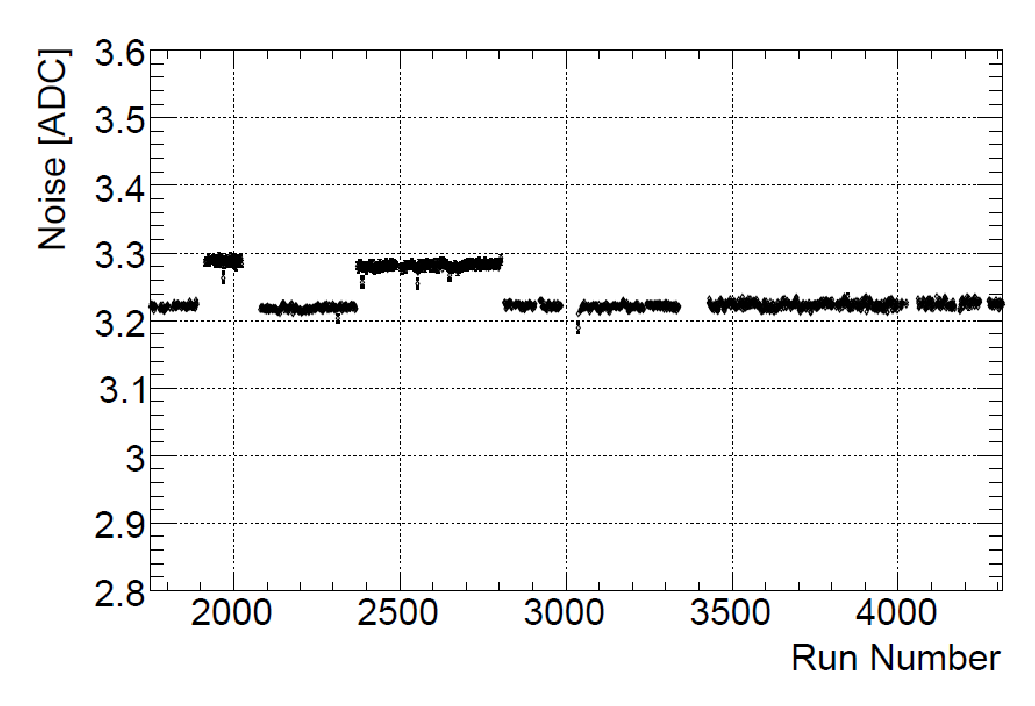
\includegraphics[width=0.8\linewidth,angle=0]{TBoverview/noise_v_run.eps}
\end{center}
\caption{Plot showing variation in the pedestal RMS, as a function of run number. The pedestal RMS is an indication of the level of noise present in the electronics, showing that this varied with time.}
\label{pedestal_variation}
\end{figure}

The default method for modeling noise in the simulation is done during the digitization step, where the autocorrelation matrix for the noise is retrieved from a database. It is then used to randomly generate the noise contributions that are added to each sample. However, during data taking the level of electronic noise present was seen to vary, as can be seen \cmt{the pedestal values }in figure~\ref{pedestal_variation}. Data for different beam configurations was taken at various times, so the average noise present for runs at a specific particle/beamspot/energy differs from that for runs with another beam configuration. 

To account for this, randomly triggered data taken from the same runs as the physics data is used to generate the noise added into the simulation, using a procedure discussed below. This method allows different beam configurations to be reconstructed with different levels of noise, whereas the default method of generating noise lacks this functionality.


%
%
%
%
%
%The default method for modeling this noise is done during the digitization step, where a randomly generated noise contribution is added to each sample. 
%
% The default method for applying this noise is to add a random amount 
%
%The default method for modeling this noise is done during the digitization step, where a randomly generated noise contribution is added to each sample. 
%
%In addition to physics data, some randomly triggered events were recorded during data taking. 
%
%
%Noise can be quantified by studying the rms of the pedestal values, which gives a value of of 3.2 ADC counts per sample when averaged over all channels and all runs. In addition to physics data, some randomly triggered events were recorded during data taking. The data taken by these random triggers is essentially all noise, and allows the correlations between samples to be studied. 
%
%
%
%
%
%Default: noise autocorrelation retrieved from database, which is used to randomly generate the noise that is added to each sample. 
%
%
%However, during data taking the level of electronic noise present was seen to vary, as can be seen from the pedestal values in figure~\ref{}.
%Runs for different beam configurations done at various times, so average noise present for specific particle/beamspot/energy will be different to that for another beam configuration. 
%To account for this, randomly triggered data taken from same runs as the physics data is used to generate noise added into the simulation, using a procedure discussed below. Default method generating noise lacks this functionality.
%
%
%
%
%
%noise observed to vary
%
%
%
%
%after event simulated, reconstruction done the same way as data, with some exceptions
%First, LarDigitMaker used to simulate electronics and turn hits into digits., which are then fed to LarRawChannelMaker.
%second is the way in which noise is handled. noise needs to be simulated in Monte Carlo. By default, this is done in digitization, random amount added to each sample. Testbeam case this is not done, instead the noise is added to the LArRawChannelBuilder algorithm.  

\subsection{Noise Generation and Application}


%As data-taking progressed, the level of noise observed in the FCal electronics was seen to vary from %run to run. \red{cause?}. Data for a different sets of run conditions (beam energy, particle type, beamspot position) taken with different level of noise present. 
%
%The RMS of the electronics noise over all runs is 3.2 ADC counts per sample for summed channels \red{and unsummed attenuated channels}. The simulation initially used this value when modeling the electronics noise during the digitization process, by adding or subtracting a random amount to each sample. However, as the level of the noise varied during data taking it was decided that the simulation should model this, and that the noise used in the simulation should reflect the noise present in the data.
%
%For a given set of data, e.g. 200GeV electrons at position 4L, data taken from randomly triggered events is used to calculate the properties of the electronics noise and model this in the simulation. The random data is used to generate a covariance matrix, describing the correlations between channels


The noise added into the simulation is derived from the randomly triggered data. A covariance matrix is generated by running over the randomly triggered data taken with a specific beam configuration (e.g. 200GeV pions directed at position 4L), such that 
\begin{equation}
M_{ij} = \frac{1}{N_\mathrm{events}}\sum_n^{N_\mathrm{events}} e_{i,n} \, e_{j,n}
\end{equation}
where $e_{i,n}$ is the noise reconstructed from the $i$-th channel of the $n$-th event, in ADC counts. The matrix $M_{ij}$ is then diagonalised, such that it can be written as
\begin{equation}
\mathbf{M} = \mathbf{U}^T \, \mathbf{D} \, \mathbf{U}
\end{equation}
where $\mathbf{U}$ is a unitary matrix with columns equal to the eigenvectors of $\mathbf{M}$, and $\mathbf{D}$ is a diagonal matrix which has the eigenvalues of $\mathbf{M}$ as its entries. The matrix $\mathbf{U}^T$ thus acts as a transformation matrix, transforming information from the ``channel'' basis to the eigenvector basis. The eigenvectors and eigenvalues are written to file, and then retrieved during the reconstruction.

The noise is applied in the LArRawChannelBuilder algorithm, after the pulse peak has been found through application of the OFCs. \cmt{sensible, as this method makes no use of information on individual samples.}The matrix $U_{ij}$ and eigenvalues $D_{ii}$ are first read from file. For each event a vector of noise, $N_i$ is then generated. This is done in the eigenvector basis using a normal distribution, such that $sigma (N_i) = D_ii$. This noise is then transformed back into channel basis, such that 
\begin{equation}
N^\prime_i = \sum_j U_{ij} \, N_j
\end{equation} 
which builds in all the correlations between channels. The noise $N^\prime_i$ is then added to the reconstructed pulse peak of the $i$-th channel.

The default method relies on an autocorrelation matrix, such that a correlations between samples are present but each channel is considered independently. The alternative method described above avoids dealing with the noise on individual samples and instead considers the total noise on the reconstructed pulse peak, while also incorporating correlations in the noise between different channels. These correlations are significant, as without them the estimations of the noise contribution in a given cluster are too low. This is important when studying the energy resolution of the FCal, which will be discussed later.


%
%
%
%
%
%
%
%
%
%
%
%
%store eigenvectors and eigen values. (check this).
%
%in ChannelBuilder, vector of noise generated in eigenvector basis. This vector is then multiplied by matrix of eigenvectors in order to transform back into the channel basis. noise then applied to each channel.
%
%method ensures that correlations in noise between channels are preserved, which does not happen in default method. Initial attempts at implement noise only focused on using the correct RMS for each channel, neglecting correlations. Clustered noise was subsequently found to be too low.
%
%
%
%diagonal
%
%   




%%\chapter{TestBeam Overview}
%%\section{Motivation}
%%\section{Beamline Setup}
%%\section{FCal Electronics}
%%10-15 pages
%
%\chapter{MC Simulation} 
%\section{Athena?}
%\section{Geometry?/G4/Simulation}
%\section{Digitization and Reconstruction}
%\subsection{Noise}
%%10-15 pages
%
%\chapter{Testbeam results}
%\section{Analysis}
%\section{Data Results}
%\section{MC Results}
%%20 pages
%HTTP://inspirehep.net/record/1082936
%
%figures are here:
%https://atlas.web.CERN.ch/Atlas/GROUPS/PHYSICS/PAPERS/STDM-2011-02/

\cmt{
todo:

2010 atlas running 

DQ - in detector chapter?

define coordinates in detector. do rapidity there too.


JP thesis

http://proquest.umi.com/pqdlink?did=1891734781&Fmt=2&VType=PQD&VInst=PROD&RQT=309&VName=PQD&TS=1338239857&clientId=79356
}





\chapter{Inclusive Jet and Dijet Cross-Sections}
\label{INCJETCHAPTER}
\section{Introduction}
\cmt{red To Do: check some things, make sure we understand stuff
choice of scale for dijets - avoids negative cross-sections. These come from negative weights, whats the deal here.

make sure we say why 0.4 and 0.6 are used - sensitivity to pileup/UE effects.

dijets - why different pt cuts for leading and subleading - (easier for theory)
}
%inclusive jet cross-section, any jet in ATLAS. Final result is a double differential cross-section for jet production, binned in rapidity and Jet \pt. Early measurement consisted of $17 nb^{-1}$, covering \pt~from x to x, and rapidity from x to x. In early 2011 the measurement was repeated, using full dataset, increasing the kinematic range covered from x to x. Extending measurement to forward rapidity meant using forward triggers, required knowledge of their behaviour. In addition, trigger scheme for transition region involved some additional complexities. (Discussed in forward trigger Section. )

%
%will first talk about jets in ATLAS and Jet calibration. Then discuss the event selection and data quality used for the analysis. Then talk about TRIGGERS, with emphasis on the forward jet triggers. Data correction talks about unfolding, then discuss results and uncertainties.
The inclusive jet cross-section refers to the cross-section for jet production with no discrimination based on the final state, i.e. all jets in each event are considered. The cross-section measurement is binned in terms of the transverse momentum, \pt, and the jet rapidity, $y$. The cross-sections studied in this chapter are significant as they represent a precise measurement of QCD in a region of phase space that has not previously been explored\footnote{The inclusive jet cross-section measurement made by CDF covers $|y| < 2.1$ and in jet rapidity and 62~GeV~$ < \pt < $~700~GeV in jet \pt~\cite{CDF_incjets}.}. Because QCD is the dominant process at the LHC, the inclusive jet and dijet cross-sections also allow jet production to be properly understood as a source of background in searches for more exotic processes, such as those presented in \cite{monojets,dijets}.
% The jet rapidity is given by
%\begin{equation}
%y = \frac{1}{2} \log \frac{E +p_z}{E - p_z}, 
%\end{equation}
%which reduces to the pseudorapidity in the limit where the jet is massless.% defined rapidity in detector chapter

The first \atlas measurement of the inclusive jet and dijet cross-sections was made in 2010 \cite{InclusivePaperAtlas1,inclusive_confnote_1}, using $17\mathrm{nb}^{-1}$ of early data collected from 7 TeV collisions. The jet production cross-section was measured for jets with \pt~from 60 to 600 GeV and with rapidities less than 2.8 in magnitude. This measurement was updated in early 2011 using the full 2010 \atlas dataset ($37\,\mathrm{pb}^{-1}$) to extend those results. This update expanded the kinematic coverage of the measurement to include jets with \pt~from 20 GeV to 1.2 TeV, and the rapidity range was extended into the forward region to include jets with $|y| < 4.4$\footnote{The FCal coverage extends out to $|\eta| < 4.9$, however an upper limit of 4.4 on the rapidity ensures that the jets under consideration were fully contained within the calorimeter}.   Figure~\ref{fig_kinematic_range} shows the kinematic region covered by the initial measurement compared to that described in this analysis. The dijet mass spectrum has also been measured using 2010 data, and the rapidity coverage of this measurement has also been expanded to include the forward region. The results discussed here have been presented as a conference note \cite{IncJetConf} and were published in 2012 \cite{InclusivePaper2010}. The inclusive jet cross-section has also been measured with the CMS detector using two independent analyses for 2010 data; the first of which covers the region $|y| < 3$ and uses  a ``particle flow'' method to reconstruct jets~\cite{CMSincjet}, while the second covers the region $3.2 < |\eta| < 4.7$ and uses jets reconstructed from the CMS forward calorimeter~\cite{CMSincjetForward}. The \atlas measurement of the inclusive jet cross-section discussed in this chapter coherently uses the same jet reconstruction technique throughout the analysis, with no gaps in the rapidity coverage. The dijet mass spectrum has also been measured at CMS, though only for jets in the region $|y| < 2.5$ \cite{CMS_dijet},whereas the \atlas dijet analysis presented here has the same rapidity coverage as the inclusive analysis ($|y| < 4.4$). 

%\cite{CMSincjet,CMSincjetForward},

Section~\ref{sec_2010_overview} gives a brief overview of the operation of \atlas and the LHC during 2010, while Section~\ref{sec::jetsinatlas} describes how jets are defined and calibrated in \atlas data. The event selection and triggers used for data collection are described in Section~\ref{sec::eventselection}, while Section \ref{sec::unfolding} describes the method used to correct for detector resolution effects in the measured data (``unfolding''). The treatment of experimental uncertainties is described in Section~\ref{sec::uncertainties}, and results are presented in Section~\ref{sec::results}. 

%
%
%
%%\red{something about dijets here}
%%
%%\red{mention dijets}
%%\red{theoretical predictions}
%
%%Initial measurement, extension, cross-section binned in terms of rapidity and Jet \pt
%%motivation, probe QCD in new kinematic regime, understanding jet backgrounds in other analyses.
%
%%will talk about Jet Reconstruction in atlas, discussing the anti-kt algorithm used. Also calibrating jets to the et Energy scale and uncertainties associated with this.
%%Will then talk about the trigger strategy used for the analysis. There are some complexities relating to jet triggers in the rapidity region from $2.8 < |y| < 3.6$, referred to as the ``transition bin'', which will be discussed in detailed in Section~\ref{IncJets_transbin}.

\begin{figure}[tbp]
\begin{center}
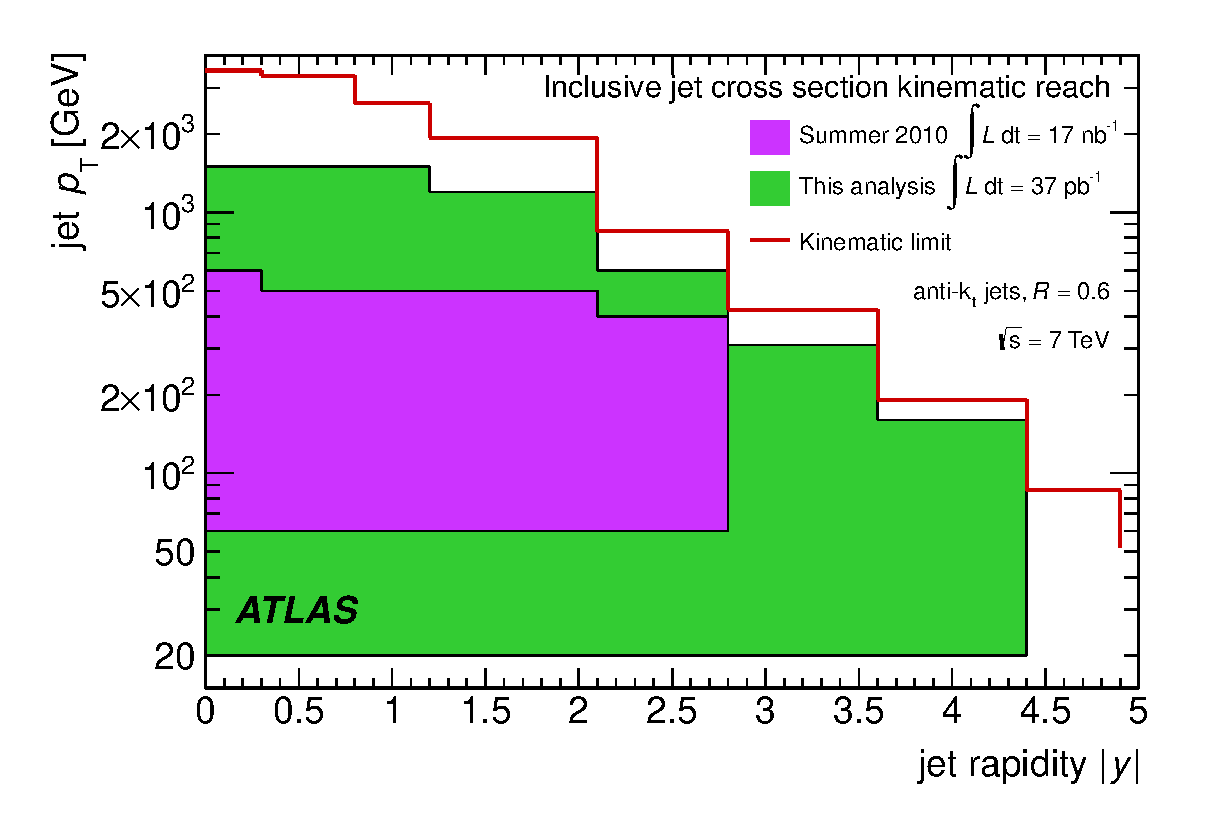
\includegraphics[width=0.8\linewidth,angle=0]{inclusive_results/figs_new/fig_01.eps}%KinematicRange}
\end{center}
%\centerline{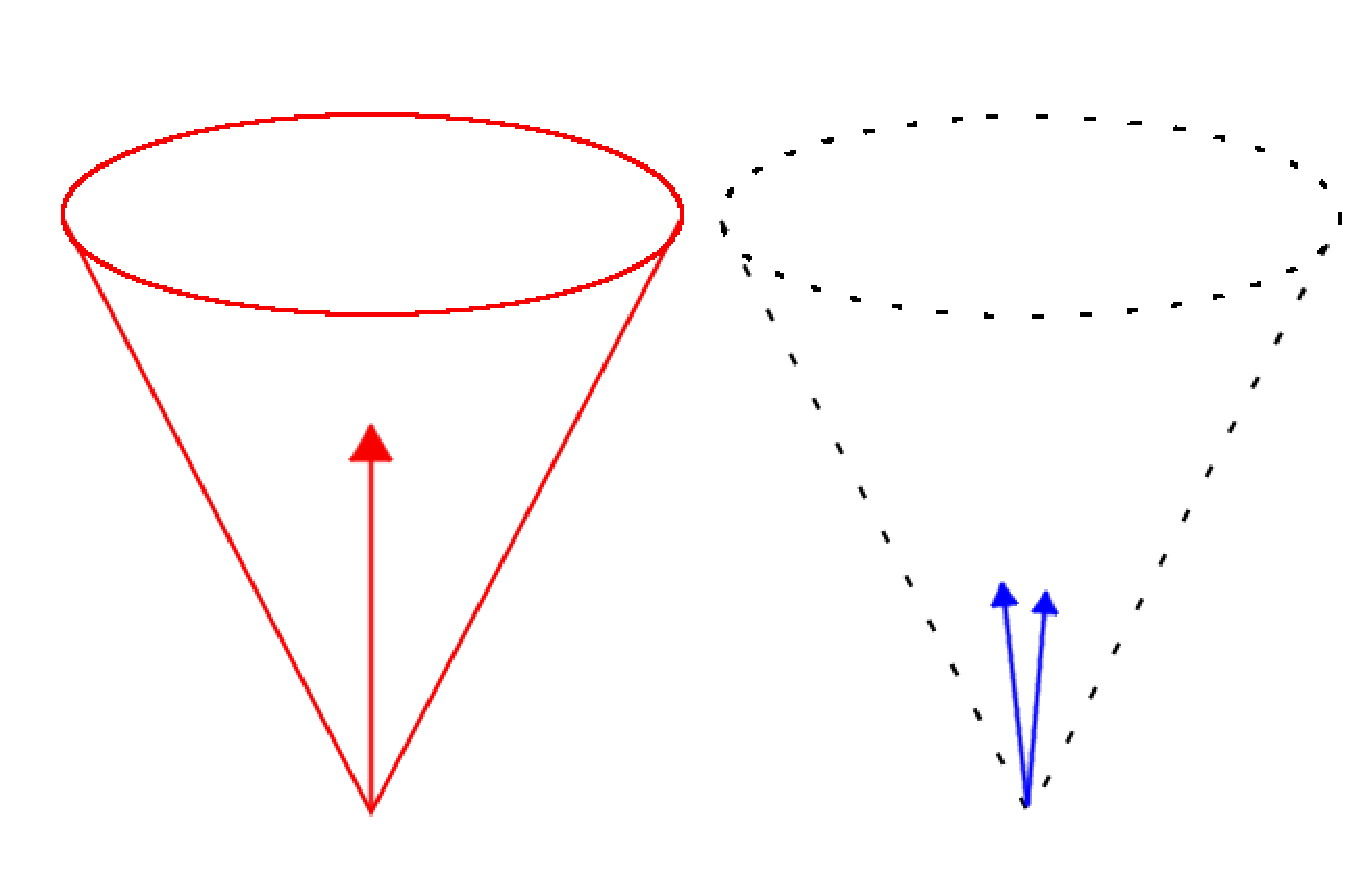
\epsfig{file=./figs/collinear.eps  , width=0.95\textwidth}}
\caption[Kinematic range of inclusive jet cross-section measurements]{Diagram showing the kinematic range covered by the first inclusive jet cross-section measurement (purple) using $17\mathrm{nb}^{-1}$ of early data, and that covered when using the full $37\mathrm{pb}^{-1}$ from the 2010 dataset (green).}
\label{fig_kinematic_range}
\end{figure}
\clearpage

\section{Overview of 2010 Running}
\label{sec_2010_overview}
%\red{took x amount of data. nine run periods (a-I), further divided into sub-periods. 2010 was the start of 7 TeV collisions, so systems were commissioned as data taking progressed. luminosity also improved over the course of the year., from XIX to YYY. size of these luminosity increases significant, as a t several points during the year the size of the 2010 was doubled within a single %run of duration $\sim$20 hours.} data taken in lumi blocks. data quality - good detector status


Data taken during 2010 has been divided into nine data periods, A-I. Each period represents an interval during which there were no major changes to the configuration of the detector and trigger, or to that of the LHC.  Each run is subdivided into a number of luminosity blocks (LB), each of which corresponds to $\sim$2 minutes worth of recorded data.
The instantaneous luminosity achieved by the LHC improved over the course of the year as the accelerator was commissioned, from $2 \times 10^{27} \mathrm{cm}^{-2} \mathrm{s}^{-1}$ early in the year to $2 \times 10^{31} \, \mathrm{cm}^{-2}\, \mathrm{s}^{-1}$ by the end of $pp$ running. \cmt{At present (Fall 2012), the LHC is running with an instantaneous luminosity is around $7 \times 10^{33}\, \mathrm{cm}^{-2}\, \mathrm{s}^{-1}$, which slightly less than the design luminosity of $10^{34} \,\mathrm{cm}^{-2} \,\mathrm{s}^{-1}$.}



%The total integrated luminosity recorded by ATLAS from $pp$ collisions in 2010 was 45$\mathrm{nb}^{-1}$. 
%, as can be seen in Figure~\ref{luminosity_fig}. Instantaneous luminosity delivered increased from $2 \times 10^{27}\, \mathrm{cm}^{-2} \,\mathrm{s}^{-1}$ initially to $2 \times 10^{31}\, \mathrm{cm}^{-2} \,\mathrm{s}^{-1}$. 

The amount of data delivered by the LHC and recorded by \atlas throughout 2010 is shown in Figure~\ref{luminosity_fig}. In total \atlas recorded 45 $\mathrm{pb}^{-1}$ of data from $pp$ collisions. Note that this value is slightly lower than the integrated luminosity delivered by the LHC (48.1 $\mathrm{pb}^{-1}$). The Inner Detector contains sensitive electronics, and so is only supplied with high voltage after stable running conditions have been established. This is the main reason for the discrepancy between the amount of data delivered and that recorded.

Certain data quality (DQ) requirements were put in place to ensure that the data used in this analysis was recorded when all relevant systems were functioning correctly. These criteria will be described in detail in Section~\ref{sec::eventselection}.  After imposing these conditions, the analysis is carried out using the remaining 37 $\mathrm{pb}^{-1}$ of data. 

%were all functioning normally. Muons not used, don't care about muons. Because of these DQ requirements, only 37$\mathrm{nb}^{-1}$ of data is used in the analysis.
%
%L1ctp solenoid, inner detector (pixel, sct, trt), calorimeters, luminosity, and tracking, jet, and missing Et reconstruction performance. Also HLT when it was in operation

%lhc stablebeams T
%725 ptag data10_7TeV
%726 dq ATLGL LBSUMM#DetStatus-v03-repro05-01 g
%727 dq L1CTP LBSUMM#DetStatus-v03-repro05-01 g
%728 dq L1CAL LBSUMM#DetStatus-v03-repro05-01 g
%729 dq atltor LBSUMM#DetStatus-v03-repro05-01 g
%730 dq atlsol LBSUMM#DetStatus-v03-repro05-01 g
%731 dq pix LBSUMM#DetStatus-v03-repro05-01 g
%732 dq sct LBSUMM#DetStatus-v03-repro05-01 g
%733 dq trtb,trte LBSUMM#DetStatus-v03-repro05-01 g
%734 dq CP_TRACKING LBSUMM#DetStatus-v03-repro05-01 g
%735 dq CP_MET_METCALO LBSUMM#DetStatus-v03-repro05-01 g
%736 dq CP_JET_JETEC LBSUMM#DetStatus-v03-repro05-01 g
%737 dq CP_JET_JETEA LBSUMM#DetStatus-v03-repro05-01 g
%738 dq CP_JET_JETB LBSUMM#DetStatus-v03-repro05-01 g
%739 dq CP_JET_JETFC LBSUMM#DetStatus-v03-repro05-01 g
%740 dq CP_JET_JETFA LBSUMM#DetStatus-v03-repro05-01 g
%741 dq LUMI LBSUMM#DetStatus-v03-repro05-01 g
%742 dq IDBS LBSUMM#DetStatus-v03-repro05-01 y+

% were put in place to ensure that all detectors and triggers relevant to this analysis were functioning properly. 
%
%quality requirements put in place to ensure that the data used in this analysis was recorded when all relevant detectors and triggers were functioning correctly.
%
%
%
%However data quality requirements meant that only 37$\mathrm{nb}^{-1}$ is used for the analysis.




\begin{figure}[tbp]
\begin{center}
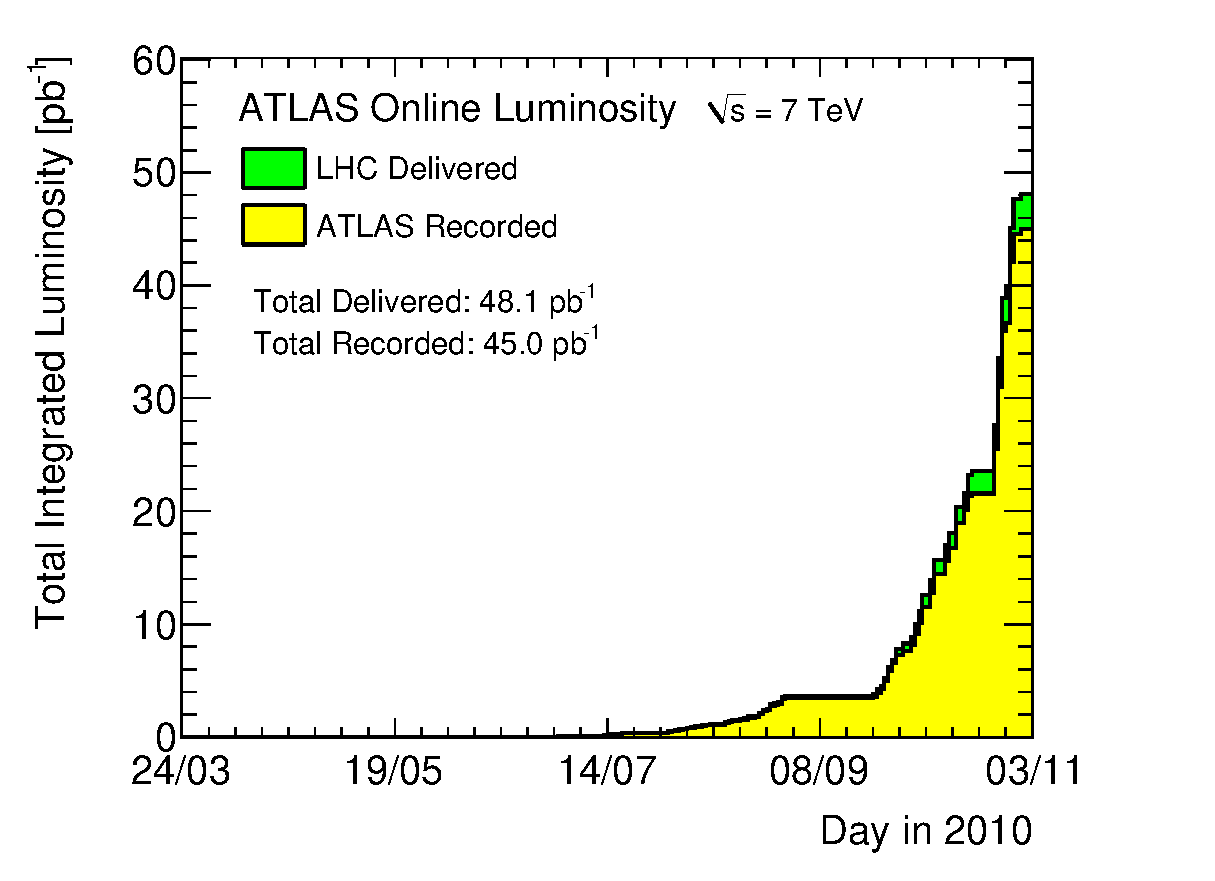
\includegraphics[width=0.8\linewidth,angle=0]{Lumi_2010.eps}
\end{center}
\caption[Integrated luminosity at ATLAS in 2010]{Integrated luminosity recorded by ATLAS over the course of 2010. }
\label{luminosity_fig}
\end{figure}

\section{Jets in ATLAS}
\label{sec::jetsinatlas}
%Jets are built from calorimeter data. 
For the inclusive jet cross-section and dijet analyses, jets were reconstructed using the \akt algorithm running on (EM scale) topological clusters of calorimeter cells. In this Section, jet finding algorithms will be presented, followed by a discussion of the jet calibration method and the uncertainty on the jet energy scale.
%\red{moved topoclusters to FCalTB chap}

\cmt{
\subsection{Topological Clustering}
\label{sec::jetsinatlas_topo}
Topological clusters (or topoclusters)  are formed by grouping neighbouring calorimeter cells based on their signal to noise ratio \cite{Lampl:1099735}. Cluster seeds are found by searching for calorimeter cells that have an energy greater than some multiple, $t_\mathrm{seed}$, of their noise RMS. The noise value used is obtained by adding in quadrature the contributions from electronics noise and pile-up. 

Neighbour cells are then added to the cluster provided they are adjacent to the seed cell and that their signal to noise ratio exceeds the neighbour threshold, $t_\mathrm{neighbour}$. This step is then repeated, with additional neighbour cells being added to the cluster if they are adjacent to an existing neighbour cell and their signal to noise ratio exceeds $t_\mathrm{neighbour}$. This is done until no new neighbour cells are found. Finally, boundary or perimeter cells are added to the cluster by taking all cells that are adjacent to neighbour or seed cells and that have a significance greater than $t_\mathrm{cell}$. 

Hadronic clusters use a ``420'' scheme, where $t_\mathrm{seed}$, $t_\mathrm{neighbour}$ and $t_\mathrm{cell}$ have values of 4,2 and 0, respectively. In this case, the signal is defined as the absolute value of the energy deposited in the calorimeter cell when searching for seed and neighbour cells. This ensures that the contribution from noise is handled symmetrically. A high value of $t_\mathrm{seed}$ makes it unlikely that a cluster will be seeded purely from noise, while a  low $t_\mathrm{cell}$  means that low  energy cells around the periphery of the shower are still clustered. A ``633'' scheme is also used in ATLAS to cluster electromagnetic objects, while other schemes have been investigated using testbeam data \cite{LouiseThesis}. Topoclusters created using the 420 scheme are used as inputs for the jet algorithms considered in this analysis.
}


\subsection{Jet Finding Algorithms}
%\red{ Italicize kt??}
\label{incjets_jetfinding}
Jet finding algorithms are run on a set of input objects, which are referred to as constituents. In general any object with an associated four-vector may be used as a constituent; however for this analysis topoclusters (discussed in Section~\ref{FCALTB_topoclusters}) are the only constituents considered\footnote{ Although ``track jets'' are used for some systematic studies and ``truth jets'' are used in the derivation of the jet calibration and in the unfolding. These use tracks and ``truth particles'', respectively, as their constituents, and will be discussed later}. The jets considered in this analysis are reconstructed using the \akt algorithm \cite{Cacciari:2008gp}. The family of \kt-like jet algorithms operate by forming a list of all the constituents in the event. For all constituents and pairs of constituents, the jet resolution quantities 
\begin{equation}
d_{ij} = \min(k_{ti}^{2p},k_{tj}^{2p}) \frac{(y_i - y_j)^2 + (\phi_i - \phi_j)^2}{R^2}
\end{equation}
and
\begin{equation}
d_i  = k_{ti}^{2p}
\end{equation}
%\end{eqnarray}
are computed, where $k_{ti}$, $\phi_i$ and $y_i$ are the transverse momentum, azimuthal angle and rapidity of the $i$-th constituent, respectively. The distance parameter $R$ is related to the desired size of the jets being found, such that the reconstructed jets will be separated by no less than $R$ in $(y,\phi)$-space. In this analysis, jets with $R =0.4$ and $R=0.6$ are studied. The parameter $p$ defines the jet-finding algorithm: $p=1$ corresponds to the \kt algorithm \cite{Catani1993187}, $p=-1$ gives the \akt algorithm, and $p=0$ corresponds to the Cambridge-Aachen cone algorithm \cite{CA_cone}. %such that found jets will be separated by no less than D in rapidity and azimuth

%\red{we use values of R=04 and R=0.6, WHY??? - larger radius, get more of the QCD radiation, but also more sensitive to underlying event.}

Once the $d_{ij}$ and $d_i$ have been computed, the values are sorted. If the smallest value present corresponds to a $d_{ij}$, then the $i$-th and $j$-th constituents are formed into a proto-jet by summing their four momenta. The proto-jet is then added to the list of constituents and its components are removed. The $d_{ij}$ and $d_i$ values are then recomputed for all remaining constituents and proto-jets. This process is repeated, with each iteration either adding constituents to an existing proto-jet or merging constituents to form a new one. In the case where a $d_i$ value is smaller than any $d_{ij}$ value, this proto-jet is taken as a complete, final jet and is removed from the list. The process continues until the constituent list is empty, with all constituents having been used to form complete jets. The four momentum of a jet is obtained by summing the four momenta of its constituents. A jet mass may then be defined by calculating the invariant mass of the jet's four momentum.


%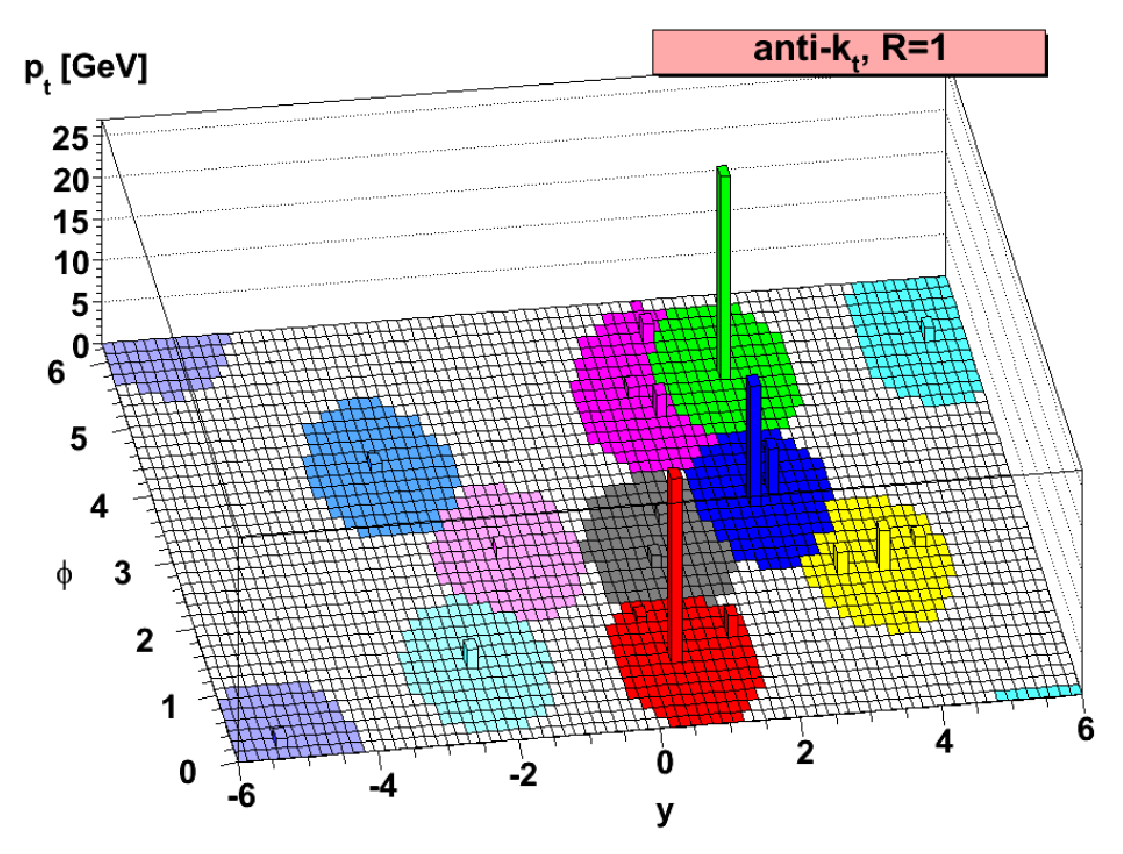
\includegraphics[scale=1]{./figs/akt_finding.eps}
%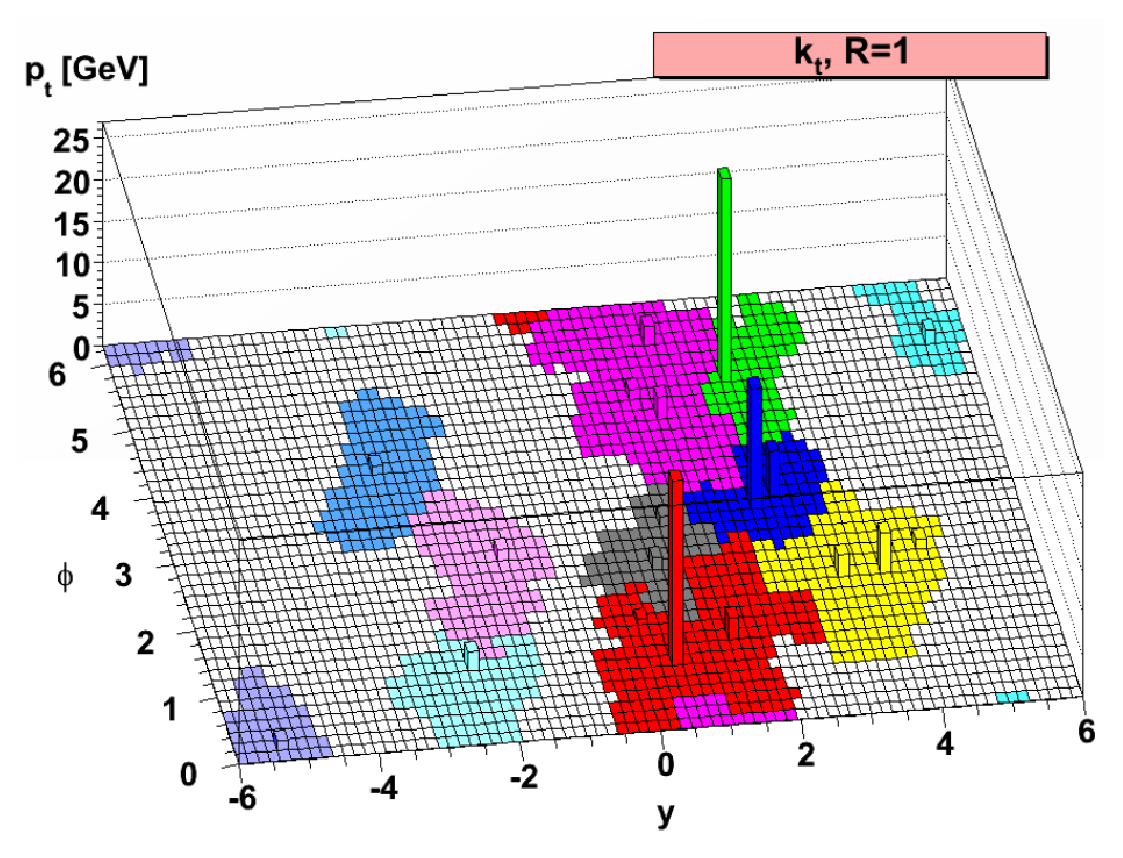
\includegraphics[scale=1]{./figs/kt_finding.eps}
%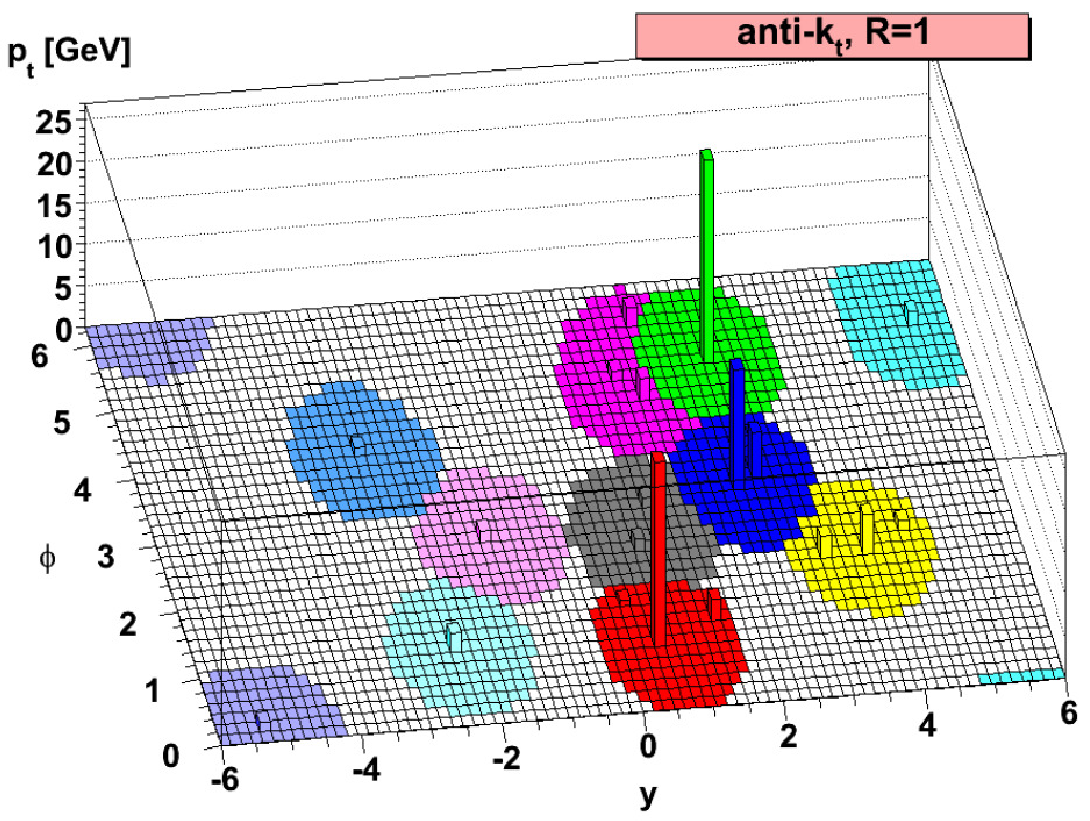
\epsfig{file=./figs/akt_finding.pdf}
\begin{figure}[hbt]
\begin{centering}
\subfigure[]{
\includegraphics[width=0.4\linewidth,angle=0]{kt_finding}
\label{fig_ktfinding}
}
\subfigure[]{
\includegraphics[width=0.4\linewidth,angle=0]{akt_finding}
\label{fig_aktfinding}
}
\caption[Comparison of \kt and \akt jet finding algorithms]{Jets found by the \kt algorithm (a) and the \akt algorithm (b). The event was generated using HERWIG \cite{Herwig}, and contains some soft radiation in addition to the high-\pt~constituents\cite{Cacciari:2008gp}.} 
%\label{fig_ktfinding}
\end{centering}
\end{figure}

In the \kt algorithm, $d_{ij}$ is approximately equal to the relative difference in transverse momentum between the two constituents $i$ and $j$, in the limit where the angle between them is small. The \kt algorithm thus clusters together constituents with similar momenta. As showering partons tend to radiate collinearly, the \kt algorithm thus acts to collect all of these radiated constituents and recombine them into a single jet. However, this procedure clusters constituents with the smallest transverse momenta first, such that high \pt~constituents may be clustered around groups of low \pt~constituents. This results in jets with irregularly shaped boundaries, as shown in Figure~\ref{fig_ktfinding}. Conversely, the \akt algorithm considers the highest \pt~constituents first and builds the proto-jets around those, resulting in conically-shaped jets (as shown in Figure~\ref{fig_aktfinding}). This also means that jets found by the \akt algorithm tend to be less sensitive to the effects of pile-up and the underlying event\cite{Cacciari:2008gp}, as the jet is first built around high \pt~constituents and the low \pt~constituents are added to it later, whereas the \kt algorithm would do the opposite.

%
%kt gathers things with similar transverse momenta, undoes QCD hadronisation/branching
%
%deals with smallest differences first. Clusters high \pt~constituents around (groups of) low ones. can give irregularly shaped jet boundaries.
%
%anti-kt similar behaviour to \kt, but clusters big things first, then adds small things to them. Produces very nice, cone shaped jets. Also tends to be insensitive to pile-up and underlying event effects.
\begin{figure}[tbp]
%\label{ir_fig}
%\includegraphics[scale=1]{./figs/ir_safety.eps}

%\centerline{\epsfig{file=./figs/ir_safety.eps  , width=0.95\textwidth}}
\begin{center}
\includegraphics[width=0.8\linewidth,angle=0]{ir_safety}
\end{center}
\caption[IR safety in jet finding algorithms]{Illustration of a jet algorithm which is not IR safe. In the Figure on the left, two distinct jets are found around the high-\pt~constituents. In the presence of soft radiation (right), the algorithm finds only a single jet.}
\label{fig_irsafety}
\end{figure}

\begin{figure}[tbp]
\begin{center}
\includegraphics[width=0.8\linewidth, height=0.3\linewidth]{collinear}
\end{center}
%\centerline{\epsfig{file=./figs/collinear.eps  , width=0.95\textwidth}}
\caption[Collinear safety in jet finding algorithms]{Illustration of an algorithm which is not collinear safe. On the left, a jet is found around a single high-\pt~constituent. On the right, the single constituent is replaced by two constituents, each with half the \pt~of the original. In this case, the algorithm fails to find a jet.}
\label{collinear_fig}
\end{figure}

%\begin{figure}[tbp]
%\begin{center}
%\subfigure[Illustration of a jet algorithm which is not IR safe. In the Figure on the left, two distinct jets are found around the high-pt constituents. In the presence of soft radiation (right), The algorithm finds only a single jet.]{\includegraphics[width=0.8\linewidth,angle=0]{ir_safety}
%\label{fig_irsafety}
%}\\
%\subfigure[Illustration of an algorithm which is not collinear safe. On the left, a jet is found around a single high-pt constituent. On the right, the single constituent is replaced by two constituents, each with half the \pt~of the original. In this case, the algorithm fails to find a jet.]{\includegraphics[width=0.8\linewidth, height=0.3\linewidth]{collinear}
%\label{collinear_fig}
%}
%\end{center}
%\end{figure}


The \kt-like jet algorithms are favored because they are both infrared (IR) and collinear safe. IR safety means that the jets found are stable with respect to the presence of low \pt~constituents arising from pile-up or the underlying event.  For an algorithm to be IR safe,  the presence of soft particles can not ``confuse'' the algorithm into mistaking two separate jets for a single large jet, as illustrated in Figure~\ref{fig_irsafety}. Collinear safety requires that the algorithm will still find a jet if, for instance, a single high-\pt~constituent is replaced by two (or more) close together constituents with lower \pt~(Figure~\ref{collinear_fig}). The \kt-like algorithms have these properties, whereas most iterative cone algorithms (such as those presented in~\cite{cones}) tend not to.


%\begin{figure}[tbp]
%\centerline{\epsfig{file=./eps_4_6_2010/Electron_resolution_4L.eps  , width=0.95\textwidth}}
%\caption{Electron Resolution at 4L }
%\end{figure}


%Anti-kt works by taking list of all constituents, and considering the quantities
%
%\begin{eqnarray}
%d_{ij} &=& \min(k_{ti}^{-2},k_{tj}^{-2}) \frac{(y_i - y_j)^2 + (\phi_i - \phi_j)^2}{R^2}\\
%d_i  &=& k_{ti}^{-2}\\
%\end{eqnarray}
%where $k_{ti}$, $\phi_i$ and $y_i$ are, respectively, the transverse momentum, azimuthal angle and rapidity of the $i$-th constituent, and $R$ is a distance parameter describing the desired size of the jets being sought after. \red{Some motivation for doing this}.


%\begin{figure}[tbp]
%\includegraphics[width=0.8\linewidth,angle=0]{jet_jetsch}
%\end{figure}
%
%\begin{figure}[tbp]
%\centerline{\epsfig{file=./figs/ir_safety.eps  , width=0.95\textwidth}}
%\end{figure}
%
%
%
%\begin{figure}%[ptb]
%  \begin{center}
%    \includegraphics[width=0.8\linewidth]{jet_jetsch}
%  \end{center}
%  \caption[Schematic view of a hard proton-proton interaction]
%          {Schematic view of a hard proton-proton interaction.\label{fig:qcdjet}}
%\end{figure}

\subsection{Jet Energy Scale Calibration}
\label{section_JES}
%
%%\blue{when saying reconstructed, do I mean before or after calibration? be consistent. Also mention why numerical inversion is used.}
%
Once a jet has been reconstructed, its energy must be calibrated to the Jet Energy Scale (JES). For this analysis, this is done  through an ``EM+JES'' scheme~\cite{JES_pub}, whereby the EM scale energy of the jet is multiplied by a calibration factor to obtain the energy at the JES.\cmt{mention EM scale? testbeam = z->ee correction?} The calibration is derived from Monte Carlo simulations using a numerical inversion process. \cmt{The jet finding algorithm is run on the final state particles produced by the event generator to form ``truth jets'', which are then compared to the reconstructed jets in the event. The calibration is chosen to maximise the agreement between the truth jets and the reconstructed jets.} %The JES calibration accounts for the following effects:
%\begin{itemize}
%\item{} \red{corrects for pile up effects.}
%\item{} non-compensation of the calorimeter, i.e. the energy is calibrated to the hadronic scale.
%\item{} energy deposited in inactive (uninstrumented) regions of the detector
%\item{} leakage effects from particle showers not fully contained in the calorimeters
%\item{} particles contained in the truth jet but not in the reco jet
%\item{} energy from showering particles that is not collected by the topoclustering algorithm. (out of cluster corrections).
%\end{itemize}
%\cmt{``Calibration'' corrects for pile up. EM+JES does not, it takes the (pile-up corrected) EM scale energy as input, and outputs the calibrated jet}

The calibration is done in three steps. First, the EM scale energy of the jet is adjusted in order to correct for pile-up effects. Additional proton-proton interactions from the same event can deposit energy in the calorimeter, affecting the energy of the high \pt~objects from the hard scattering. Minimum bias data are used to determine the average energy deposited in the calorimeter as a function of pseudorapidity and the number of primary vertices reconstructed from the event. This information is used to subtract the average EM scale energy added to the jet as a result of pileup.

The second step is to correct the kinematics of the jet, still at the EM scale, based on the location of the hard scattering. Initially, jet kinematics are computed using the geometrical centre of \atlas as the origin of the jet. The luminous region of \atlas has a width of $\sim 40-70 \mu \mathrm{m}$ in the transverse directions and $\sim 22$ mm longitudinally \cite{beamspot_2010}, and it is within this volume that the hard scatterings occur. The vertex with the highest sum of squared transverse momenta from tracks ($\sum p_{\mathrm{T},track}^2$) is taken as the position of the hard scatter, and all jet kinematic quantities ($p_\mathrm{T},y,\phi$, etc.) are recomputed using this vertex as the origin. \cmt{ improves angular resolution, improved \pt~response}

Finally, the JES correction is applied. The correction is derived exclusively from Monte Carlo, using samples generated without the inclusion of pile-up. An event generator is used to simulate a hard parton-parton scattering typical of proton-proton collisions, which outputs a set of final state particles and their four momenta. \geant is then used to simulate the interactions of these particles with the detector. The event is then reconstructed using the same methods that are used for the data: calorimeter cells are reconstructed and used to form topological clusters, on which jet finding algorithms are run. ``Truth'' jets are formed by running the jet finding algorithms on the final state particles output by the event generator. 

The JES calibration accounts for the following effects:
\begin{itemize}
%\item{} \red{corrects for pile up effects.}
\item{} non-compensation of the calorimeter, i.e. the energy is calibrated to the hadronic scale;
\item{} energy deposited in inactive (uninstrumented) regions of the detector, such as cryostat walls or support structures;
\item{} leakage effects from particle showers not fully contained in the calorimeters;
\item{} particles contained in the truth jet but not in the reconstructed jet;
\item{} energy from showering particles that is not collected by the topoclustering algorithm (out of cluster corrections).
\end{itemize}
\cmt{EM+JES is the whole thing. JES is the final step. Offset (pileup) and origin are part of EM JES. the JES part corrects for the above things.}

The calibration is derived by comparing the jets reconstructed from the (simulated) calorimeter information to the truth jets. A reconstructed jet is matched to a truth jet if the distance between them satisfies $\Delta R < 0.3$, where $\Delta R = ( \Delta \eta^2 + \Delta \phi^2 )^{1/2}$.
%  is less than 0.3 in $(y,\phi)$. 
%To avoid mis-matching jets, only isolated jets are matched:
Jets are only considered if they are isolated in order to avoid mis-matching in cases where multiple jets are close together. A reconstructed/truth jet must have no other jets with $p_\mathrm{T,EM} > 7 $GeV within $2.5R$, or it is not used in the derivation of the calibration. 

The matched reconstructed-truth jet pairs are then used to define the response $R$, such that 
\begin{equation}
R = \frac{E_\mathrm{reco}^\mathrm{EM}}{E_\mathrm{truth}},
\end{equation}
where $E_\mathrm{reco}^\mathrm{EM}$ is the EM scale energy of the reconstructed jet and $E_\mathrm{truth}$ is the energy of the truth jet. The response is binned in $E_\mathrm{truth}$ and $\eta_\mathrm{det}$, the pseudorapidity of the reconstructed jet at the EM scale. 
For each $(E_\mathrm{truth},\eta_\mathrm{det})$ bin, the mean reconstructed jet energy, $\langle E_\mathrm{reco}^\mathrm{EM} \rangle$, is found, and a Gaussian fit is used to extract the mean response, $\langle R \rangle$. 

The response is then parameterised as a function of $E_\mathrm{reco}^\mathrm{EM}$ for each $\eta_\mathrm{det}$ bin. 
%This is done
For the $k$-th $\eta_\mathrm{det}$ bin, a fit is performed on the $(\langle E_\mathrm{reco}^\mathrm{EM} \rangle,\langle R \rangle)$ points obtained from each $E_\mathrm{truth}$ bin. The fitted function is of the form

\begin{equation}
F_{\mathrm{calib},k}(E_\mathrm{reco}^\mathrm{EM}) = \sum_{j=0}^{N_\mathrm{max}} a_j \left(\log E_\mathrm{reco}^\mathrm{EM}\right)^j,
\end{equation}
where the $a_j$ are free parameters and $N_\mathrm{max}$ is an integer between 1 and 6, depending on $\eta_\mathrm{det}$.

The correction factor is then found by inverting $F_{\mathrm{calib},k}$, so the final EM+JES energy of a jet lying in the $k$-th $\eta_\mathrm{det}$ bin is given by

\begin{equation}
E_\mathrm{reco}^\mathrm{JES} = \frac{E_\mathrm{reco}^\mathrm{EM}}{F_{\mathrm{calib},k}(E_\mathrm{reco}^\mathrm{EM})}.
\end{equation}




\cmt{

mention this:
The present calibration scheme, EM+JES, calibrates the reconstructed jets using energy and  dependent
correction factors derived from simulated Pythia events.4 To derive the correction factors, particle
jets, reconstructed using the Monte Carlo (MC) event record, are matched with jets reconstructed in the
calorimeter, and the correction is calculated by dividing the true particle jet energy by the EM-scale
energy of the matching calorimeter jet.5 Following this, a small -dependent correction is applied to remove
a bias in the reconstructed  of jets that occurs when jets fall in specific regions of the calorimeter
that have a much lower response than the regions around it. The reason for this bias is that jet directions
are reconstructed using the \pt-weighted sum of the constituents directions. The bias occurs when some
of the constituent particles fall into a crack region with low response, and the jet is pulled toward the
region with the higher response.
 }

%A Gaussian fit is made for each $(E,\eta)$ bin from which the mean response, $\langleR\rangle$ is extracted.  


\cmt{
compare truth and reco
ratio R = Ereco/Etruth, binned in Etruth and ndet (reco)
for each bin, mean response <R> is derived from a Gaussian fit and mean <Ereco> is found. 

for each ndet bin, function F is fit to the (<Ereco>,<R>) points( i.e. 1 point for each Etruth bin)

fit function F has form F(Ereco) = \sum_i^Nmax a_i (\log Ecalo)^i 
Nmax chosen between 1 and 6 to maximise goodness of fit.

Final calibration is then just 1/F, i.e.

E_reco(EM+JES) = E_reco(EM)/F|ndet

}


 



\cmt{ 

 Only isolated jets are considered when deriving the calibration, where a jet is considered isolated if no other jets with Em \pt~above 7GeV lie within $2.5R$, where $R$ is the jet radius. Reconstructed jets are then matched to truth jets

 Only isolated jets are considered when deriving the calibration, If two or more jets with EM scale \pt~above 7GeV lie within 2.5R then they are ignored.

Only isolated jets are used when deriving the calibration, so that jets excluded if another jet lies within 2.5R in y,phiOnly isolated jets are considered, A reconstructed jet and truth jet that are separated by $Delta R < 0.3$ are considered to be matched, provided there are no other . 


Truth jets and reconstructed jets within $\DeltaR < 0.3$ of each other are considered to be matched, provided the jets are isolated. A jet is considered isolated if there are no other jets with an EM scale energy above 7 GeV within 2.5$R$ in ($y,\phi$), where $R$ is the radius used in the jet-finding algorithm.  

Then take the ratio of \pt_reco/PT_truth

Calorimeter Jets?

isolated jets nothing over 7 GeV (EM) within 2.5R
matched DR< 0.3
}




\cmt{

Use EM+JES scheme
start at EM, then apply weight
weight comes from MC (numerical inversion)
EM scale originally derived from testbeam
updated/corrected using z->ee data.


weight accounts for 

calorimeter non-compensation (hadronic scale)
dead material
leakage (particles out the back)
particles in truth jet but not in reco jet (out of cone?)
out of cluster corrections/out of jet corrections? (different from above?)

before weighting is carried out, correction is applied to jet energy at EM scale in order to take into account pile up. This correction is parameterised as a function of the number of primary vertices measured in the event and the pseudorapidity of the jet.



\^
1. correct for pileup
2. correct jet kinematics - rapidity and phi recalculated from primary vertex, rather than centre of ATLAS.
3. Numerical inversion

origin correction improves jet angular resolution - improves \pt~response 


Mention Global Cell weighting/local hadronic weighting?

}




\subsection{JES uncertainty}
\label{JES_uncertainty_section}
The systematic uncertainty on the JES is an important quantity, and one of the dominant sources of uncertainty in the inclusive jet and dijet cross-section analyses. There are several sources that contribute to this uncertainty, outlined below:

\begin{itemize}
\item{\bf Relative calibration of uncertainties between forward and central regions.} Contributions to the JES uncertainty from the sources discussed below have been calculated in the central region, $0.3 < |\eta | < 0.8$. This uncertainty is used as a baseline, and an intercalibration method \cite{ATLAS-CONF-2011-014} is used to extend the estimate of the JES systematic into other pseudorapidity regions. This method uses a \pt~balancing technique applied to dijet events in order to obtain the ratio of the calibrated jet responses in different regions of pseudorapidity. This response was calculated for data and simulation, using several different MC event generators. The RMS of the differences in response between MC and data is then added in quadrature to the baseline uncertainty, yielding the uncertainty in higher pseudorapidity regions.
\item{\bf Uncertainty from the calibration method} The EM+JES method calibrates jets by applying a correction factor to the EM scale energy of the jet. This treats all of the jets constituents equally, i.e. each constituent is effectively scaled by the same calibration factor. Additionally, this same correction factor is used for both the energy and transverse momenta of the jet, which may bias the calibrated \pt~in cases where the calibrated jet mass differs from the mass of the truth jet. The uncertainty arising from the calibration method is estimated by comparing the reconstructed jets at the EM+JES scale to their truth jet counterparts. The responses $\langle R_E \rangle = \langle E_\mathrm{reco}^{EM+JES} / E_{truth} \rangle$ and $\langle R_P \rangle = \langle p_\mathrm{T,reco}^{EM+JES} / p_\mathrm{T,truth} \rangle$ are computed, and binned in terms of $p_\mathrm{T,reco}^{EM+JES}$ and $|\eta|$. Any deviation of $\langle R_E \rangle$ or $\langle R_P \rangle$ from unity suggests that the kinematics of the reconstructed jets after calibration are not equal to those of the truth level jets (this is called ``non-closure'')\cmt{, for the reasons mentioned above}. The estimated uncertainty associated with the calibration method is taken as the largest deviation of $\langle R_E \rangle$ or $\langle R_P \rangle$ from unity, and is found to be less than 1\% for $p_\mathrm{T,reco}^{EM+JES} > 30$ GeV and less than 2\% for 30 GeV $> p_\mathrm{T,reco}^{EM+JES} >$ 20 GeV \cite{ATLAS_JES_2010}.

\item{ \bf Uncertainty from calorimeter response} The contribution to the JES systematic from the uncertainty in the calorimeter response is derived from single particle measurements. The uncertainty in the response to charged hadrons is measured in $E/p$ studies \cite{ATLAS-CONF-2011-028} and in testbeam data \cite{Khramov:1172156}. The simulation framework allows the particles in the truth jet to be associated with the energy they deposit in the calorimeter, and thus the single particle response uncertainties can be propagated to obtain an uncertainty for the response of the jet. When estimating this uncertainty, effects relating to the calorimeter acceptance, charged particles with $E> 400GeV$\footnote{Charged particles at these energies could not be studied in beam tests, and so the uncertainties associated with particularly high energy densities or longitudinal leakage must be estimated.}, and energy deposited by neutral hadrons are also considered. Effects related to the calorimeter response are found to contribute $1.5\% -  4\%$ to the JES systematic uncertainty.

\item{\bf Uncertainty due to noise thresholds in detector simulation} The noise present in the calorimeter electronics can change over time, whereas the noise used in the simulation is fixed when the MC sample is generated. The value of the noise RMS used influences which cells are grouped into topoclusters, and thus contribute energy to the jet. The effect of the noise threshold in the simulation was studied by increasing and decreasing the noise thresholds for the topoclustering algorithm by amounts of 5-10\%. The uncertainty assigned to this effect was found to be negligible for jets with \pt~$>$ 45 GeV, and is estimated as 1\% for jets with momentum in the range 30 GeV $\leq \pt \leq$ 45 GeV. For jets with 20~GeV~$\leq \pt \leq 30$~GeV, the uncertainty was estimated as 1\% (2\%) for jets with radius 0.4 (0.6).

%The noise RMS for each cell was measured from data, and these values were then used to define the noise thresholds when reconstructing topoclusters in the simulation. Using the noise thresholds obtained from data had a similar effect to that seen when increasing the default simulation noise thresholds by 7\%. 
%
%
%The effect of the noise threshold in the simulation was measured by \red{increasing} the noise thresholds for the topoclustering algorithm by amounts of 5-10\%. This influences which cells are grouped into topoclusters, and thus contribute energy to the jet. The uncertainty assigned to this effect was found to be negligible for jets with \pt~$>$ 45 GeV, and is estimated as 1-2\% for jets with lower \pt. \red{down to 20 GeV or 30 GeV?}
%
%re-read this as
%
%use noise RMS from data in simulation, reconstruct jets using this noise threshold for topoclusters
%
%increase noise thresholds by 7\% this has the same effect as using data. Symmetric, raising/lowering by 7\% suggests the effect is symmetric.
%
%
%
%\red{1\% (2\%) for jets with $R$ = 0.4 (0.6) with 20 GeV< \pt~< 30GeV, 1\% for 30 < \pt~< 45 GeV.}

\item{ \bf Effect of additional material in simulation} As the JES calibration is intended to correct for the effects of inactive material, it is sensitive to the material description of the detector in the simulation. The effects of this were estimated by adding additional material to the simulation geometry in several places, and comparing the response obtained with the modified geometry to that obtained using the nominal geometry. 
%The variation of the energy response was found to be within 3\%, while that of the $p_T$ response was within 2\%. 
\item{ \bf MC event generators}
The nominal MC sample used in the derivation of the JES was generated using \pythia, using the AMBT1 tune. Samples were also produced using \alpgen~\cite{alpgen} interfaced with \herwig and \jimmy, and using the Perugia2010 tune for \pythia. The \alpgen sample used the CTEQ6.1 PDF set, and treated parton showering and hadronisation effects differently than the nominal \pythia sample, whereas the Perugia2010 sample provided a different treatment of the underlying event. Deviations between the response obtained from the Perugia2010 and \alpgen+\herwig+\jimmy samples with respect to the nominal \pythia sample were used to estimate the uncertainty arising from the choice of physics models. \cmt{define these in QCD chapter, event generators}

%Pythia with Perugia2010 -> underlying event uncertainty
%
%alpgen+herwig+jimmy with CTEQ6.1 -> parton showering,hadronisation,pdfs 




\end{itemize}

The total JES uncertainty, and its components, are plotted in Figure~\ref{JES_uncertainty_figs} for $R=0.6$ jets. The uncertainty in the calorimeter response is the dominant contribution to the JES uncertainty for jets with \pt~$\geq$ 100 GeV. In the central region ($0.3 < |\eta| < 0.8$), the uncertainties associated with alternative MC generators dominate below 100 GeV, while in other pseudorapidity regions intercalibration effects dominate at low \pt. At high \pt~(near the kinematic limit) the JES uncertainty is around 3-5\% in each rapidity region. The uncertainty associated with jets of radius $R=0.4$ is generally similar to that associated with jets of radius $R=0.6$.

% The dominant contribution to the JES uncertainty for in the central region ($0.3 < |\eta| < 0.8$) is from the uncertainty in the calorimeter response. In other pseudorapidity regions the intercalibration uncertainty dominates at low \pt.
 
 
%\begin{figure}[tbp]
%\begin{centering}
%\includegraphics[width=0.45\linewidth,angle=0]{JES_fig_10} 
%\end{centering}
%\caption{}
%\label{JES_uncertainty_1_fig}
%\end{figure}
%
%\begin{figure}[tbp]
%\begin{centering}
%\subfigure{
%\includegraphics[width=0.45\linewidth,angle=0]{JES_fig_10}
%\label{JES_uncertainty_2_fig}
%}
%\subfigure{
%\includegraphics[width=0.45\linewidth,angle=0]{JES_fig_11}
%\label{JES_uncertainty_3_fig}
%}
%\end{centering}
%\label{JES_uncertainty_figs}
%\end{figure}
% \red{ update these plots, see int note}
%\begin{figure}[tbp]
%\centering
%\includegraphics[width=0.85\linewidth,angle=0]{JESUncertainty_AntiKt6Topo_EMJES03-08.eps} 
%
%\caption{JES uncertainty in the central barrel region ($0.3 < |\eta | < 0.8$)}
%\label{JES_uncertainty_1_fig}
%\end{figure}
%
%\begin{figure}[tbp]
%\centering
%%\subfigure[caption 1]{
%%\includegraphics[width=0.85\linewidth,angle=0]{JES_fig_09}
%%\label{JES_uncertainty_1_fig}
%%}\\
%\subfigure{
%\includegraphics[width=0.85\linewidth,angle=0]{JESUncertainty_AntiKt6Topo_EMJES21-28.eps}
%\label{JES_uncertainty_2_fig}
%}\\
%
%\subfigure{
%\includegraphics[width=0.85\linewidth,angle=0]{JESUncertainty_AntiKt6Topo_EMJES36-45.eps}
%\label{JES_uncertainty_3_fig}
%}
%\caption{ JES uncertainty for  the end-cap  ($2.1 < |\eta | < 2.8$)  and FCal ($3.1 < |\eta | < 4.5$). At low \pt, the intercalibration provides the dominant source of uncertainty.} 
%\label{JES_uncertainty_figs}
%\end{figure}

%\begin{figure}[tbp]
%\begin{center}
%\subfigure[]{\includegraphics[width=0.6\linewidth,angle=0]{inclusive_results/figs_new/JES_3_8.eps}
%\label{JES_uncertainty_1_fig}} \\
%\subfigure[]{
%\includegraphics[width=0.6\linewidth,angle=0]{inclusive_results/figs_new/JES_21_28.eps}
%\label{JES_uncertainty_2_fig}
%}\\
%\subfigure[]{
%\includegraphics[width=0.6\linewidth,angle=0]{inclusive_results/figs_new/JES_36_45.eps}
%\label{JES_uncertainty_3_fig}
%}
%\end{center}
%\caption[Jet Energy Scale systematic uncertainty]{Systematic uncertainty on the Jet Energy Scale for jets in the regions (a) $0.3 < |\eta| < 0.8$, (b) $2.1 < |\eta| < 2.8$, (c) and $3.6 < |\eta| < 4.5$ \cite{ATLAS_JES_2010} }
%\label{JES_uncertainty_figs}
%\end{figure}
\begin{figure}[tbp]
\begin{center}
\subfigure[]{\includegraphics[width=0.6\linewidth,angle=0]{JES_new/fig_22a.eps}
\label{JES_uncertainty_1_fig}} \\
\subfigure[]{
\includegraphics[width=0.6\linewidth,angle=0]{JES_new/fig_22b.eps}
\label{JES_uncertainty_2_fig}
}\\
\subfigure[]{
\includegraphics[width=0.6\linewidth,angle=0]{JES_new/fig_22c.eps}
\label{JES_uncertainty_3_fig}
}
\end{center}
\caption[Jet Energy Scale systematic uncertainty]{Systematic uncertainty on the Jet Energy Scale for jets in the regions (a) $0.3 < |\eta| < 0.8$, (b) $2.1 < |\eta| < 2.8$, (c) and $3.6 < |\eta| < 4.5$ \cite{JES_pub} }
\label{JES_uncertainty_figs}
\end{figure}


%\caption{JES uncertainty in the central barrel region ($0.3 < |\eta | < 0.8$)}
%\label{JES_uncertainty_1_fig}
%\end{figure}
%
%\begin{figure}[tbp]
%\centering
%%\subfigure[caption 1]{
%%\includegraphics[width=0.85\linewidth,angle=0]{JES_fig_09}
%%\label{JES_uncertainty_1_fig}
%%}\\
%\subfigure{
%\includegraphics[width=0.85\linewidth,angle=0]{JESUncertainty_AntiKt6Topo_EMJES21-28.eps}
%\label{JES_uncertainty_2_fig}
%}\\
%
%\subfigure{
%\includegraphics[width=0.85\linewidth,angle=0]{JESUncertainty_AntiKt6Topo_EMJES36-45.eps}
%\label{JES_uncertainty_3_fig}
%}
%\caption{ JES uncertainty for  the end-cap  ($2.1 < |\eta | < 2.8$)  and FCal ($3.1 < |\eta | < 4.5$). At low \pt, the intercalibration provides the dominant source of uncertainty.} 
%\label{JES_uncertainty_figs}
%\end{figure}




\cmt{


There are a number of contributions to the systematic uncertainty on the JES. 

comparison of in situ and single pion testbeam measurements

dead material budget (and uncertainty)

noise?

Monte Carlo


effects of these things are estimated using MC, by varying the item in question and observing how things vary.


1. uncertainty from the calibration method
2. uncertainty in calorimeter response
3. uncertainty in detector simulation (dead material)
4. uncertainty due to event generator/physics model
5. uncertainty in relative calibration

1. looking at nominal sample in eta, \pt, response (calibrated/truth) shows small deviations from unity (non-closure). 
method assumes that every constituent requires same average correction.
same correction factor for energy and \pt~is used. In cases where the calibrated jet mass is not equal to the truth jet mass, this correction results in a bias in \pt~calibration.

uncertainty taken as largest deviation of response (in \pt~and energy) from unity,
 is ~ 2\% for jets at low \pt~in barrel, less than 1\% for jets with \pt~> 30GeV elsewhere 

non-closure and non-unity of the response are treated as different things???

uncertainty in calorimeter response. E/P measurement propagated to JES. 1.5-4\%, depending on jet \pt.

Detector simulation:
*noise
1\% (2\%) for \akt jets with R=0.4 (R=0.6) for 20 GeV < \ptJet < 30 GeV
1\% for 30 GeV <ptjet<  45 GeV
negligible above 45 GeV

*dead material
vary amount of dead material, measure effect on jet response.
uncertainties due to relative calibration between barrel and end-cap/forward region


inter calibration for forward jets??
}

\subsection{Jet Selection}

%After jets have been calibrated, there are some criteria that they need to meet before being included in the analysis. Certain detector issues are capable of causing a jet to be reconstructed even if there were no physical particles depositing energy in that region of the calorimeter. Alternatively, other particles such as electrons or cosmic muons may be mistakenly reconstructed as jets. Jet ``cleaning'' cuts were made to address these issues, and remove from the analysis as many ``fake'' jets as possible. The jet cleaning cuts, and the problems they are intended to address, are listed below

%After jets have been calibrated, they are required to pass ``cleaning cuts'' before being included in the analysis. These criteria are intended to reject ``fake'' jets that do not originate from physical energy deposits resulting from proton-proton collisions.

After jets have been calibrated, they are required to pass ``cleaning cuts'' before being included in the cross-section analysis. The cleaning cuts are intended to reject ``fake'' jets, which can be reconstructed from calorimeter signals that do not originate from proton proton collisions.  The most significant sources of these fake jets are coherent noise in the EMB, noise bursts in the HEC, cosmic rays, and beam background events. The cleaning cuts used to reject fake jets are summarised below:




%There were several detector issues that occurred during data taking which could cause the and adversely effected the The cleaning cuts are summarised below.


%	// EM coherent noise
%	//medium
%	if ((myemf>0.90) &&(fabs(myLArQuality) >0.8) && (fabs(EMscale_JetEta) <2.8)) clean = false;
%	
%	// HEC spike
%	//loose
%	if ((myhecf > 0.5 )&& (fabs(myHECQuality)>0.5) ) clean = false;
%	if (fabs(myNegativeE) >60000.0) clean = false;
%	//medium
%	if ((1 - fabs(myHECQuality) )< myhecf) clean = false;
%	
%	
%	//cosmics / beam background
%	if (fabs(myTiming)>10) clean = false;
%	if ((myemf < 0.05 )&& (mychf < 0.1)&& (fabs(EMscale_JetEta) < 2.0)) clean = false; // medium
%	if ((myemf < 0.05 )&& (fabs(EMscale_JetEta) > 2.0)) clean = false;
%	if (myfMax > 0.99 && fabs(EMscale_JetEta) < 2.0) clean = false;
%	// medium
%	if ((myemf > 0.95 )&& (mychf < 0.05)&& (fabs(EMscale_JetEta) < 2.0)) clean = false;

\begin{itemize}
\item{\bf Coherent noise in the EM calorimeter:} Jet candidates with $|\eta| < 2.8$ were rejected if \cmt{$EM_\mathrm{f}$} $f_\mathrm{em}$, the fraction of the jet energy deposited in the EM calorimeter, exceeded 0.9 while the LAr quality variable exceeded 0.8. The LAr quality is defined as the fraction of jet cells located in the EM calorimeter that have a pulse shape significantly different to that expected.
\item{\bf Noise bursts (``spikes'') in the HEC:} Jet candidates were rejected if the fraction of the jet energy deposited in the HEC was greater than $1 - HECQ$, where $HECQ$ is the HEC quality variable, defined as the fraction of the jets cells located in the HEC that have a pulse shape significantly different to that expected. Jets were also rejected if the sum of negative energy cells exceeded 60 GeV in magnitude.
\item{\bf Cosmics rays/beam background:} Jet candidates were rejected if the average timing for jet cells was greater than 10ns from the average event time, or if 99\% of the jet energy was deposited in a single layer of the calorimeter. For jets with $|\eta| < 2.0$, tracking information can be used to define the charged fraction, \cmt{$Chf$}$f_\mathrm{ch}$, which is the fraction of the jet \pt~associated with tracks in the inner detector. In this case, jets were rejected if $f_\mathrm{ch} < 0.1$ and $f_\mathrm{em} < 0.05$ or if $f_\mathrm{em} > 0.95$ and $f_\mathrm{ch} < 0.05$. Jets with $|\eta| > 2.0$ were rejected if $f_\mathrm{em} < 0.05$.
\end{itemize}

Jet candidates which failed these cleaning cuts were excluded from the analysis. The efficiency of these cleaning cuts for real jets was at least 96\% for jets with \pt~$> 20$~GeV, and greater than 99\% for jets with \pt~$>$~60~GeV. In kinematic regions where the jet cleaning efficiency was less than 99\%, the inefficiency is corrected for in the inclusive jet and dijet cross-section measurements.

%\clearpage
\section{Event Selection and Data Quality}
\label{sec::eventselection}
%%used full 2010 dataset, $45pb^{-1}$ before DQ, 37 after. Dq cuts require stable beams, all systems go, flag bad lumi blocks from noise bursts(\red{in HEC?}). SM GRL
%\red{DATA QUALITY DATA QUALITY DATA QUALITY}
%https://twiki.cern.ch/twiki/bin/viewauth/AtlasProtected/SMJetAnalysis2010#Good_Runs_List
%%lhc stablebeams T
%%725 ptag data10_7TeV
%%726 dq ATLGL LBSUMM#DetStatus-v03-repro05-01 g
%%727 dq L1CTP LBSUMM#DetStatus-v03-repro05-01 g
%%728 dq L1CAL LBSUMM#DetStatus-v03-repro05-01 g
%%729 dq atltor LBSUMM#DetStatus-v03-repro05-01 g
%%730 dq atlsol LBSUMM#DetStatus-v03-repro05-01 g
%%731 dq pix LBSUMM#DetStatus-v03-repro05-01 g
%%732 dq sct LBSUMM#DetStatus-v03-repro05-01 g
%%733 dq trtb,trte LBSUMM#DetStatus-v03-repro05-01 g
%%734 dq CP_TRACKING LBSUMM#DetStatus-v03-repro05-01 g
%%735 dq CP_MET_METCALO LBSUMM#DetStatus-v03-repro05-01 g
%%736 dq CP_JET_JETEC LBSUMM#DetStatus-v03-repro05-01 g
%%737 dq CP_JET_JETEA LBSUMM#DetStatus-v03-repro05-01 g
%%738 dq CP_JET_JETB LBSUMM#DetStatus-v03-repro05-01 g
%%739 dq CP_JET_JETFC LBSUMM#DetStatus-v03-repro05-01 g
%%740 dq CP_JET_JETFA LBSUMM#DetStatus-v03-repro05-01 g
%%741 dq LUMI LBSUMM#DetStatus-v03-repro05-01 g
%
%find run 166466-166964 and
%partition ATLAS
% and db DATA
%  and 
%  lhc stablebeams T and 
%  ptag data10_7TeV
%dq ATLGL LBSUMM#DetStatus-v03-repro05-01 g // someone looked at DQ stuff
%dq L1CTP LBSUMM#DetStatus-v03-repro05-01 g // no clock/data header problems
%dq L1CAL LBSUMM#DetStatus-v03-repro05-01 g  // trigger good
%dq atltor LBSUMM#DetStatus-v03-repro05-01 g //toroid
%dq atlsol LBSUMM#DetStatus-v03-repro05-01 g // solenoid
%dq pix LBSUMM#DetStatus-v03-repro05-01 g //pixel
%dq sct LBSUMM#DetStatus-v03-repro05-01 g // sct
%dq trtb,trte LBSUMM#DetStatus-v03-repro05-01 g /trt 
%dq CP_TRACKING LBSUMM#DetStatus-v03-repro05-01 g // tracking (vertex reconstruction?)
%dq CP_MET_METCALO LBSUMM#DetStatus-v03-repro05-01 g // missing ET from calo (not muons)
%dq CP_JET_JETEC LBSUMM#DetStatus-v03-repro05-01 g //
%dq CP_JET_JETEA LBSUMM#DetStatus-v03-repro05-01 g //
%dq CP_JET_JETB LBSUMM#DetStatus-v03-repro05-01 g //
%dq CP_JET_JETFC LBSUMM#DetStatus-v03-repro05-01 g //
%dq CP_JET_JETFA LBSUMM#DetStatus-v03-repro05-01 g // jet reconstruction good
%dq LUMI LBSUMM#DetStatus-v03-repro05-01 g // luminosity monitoring
%dq TRJET LBSUMM#DetStatus-v03-repro05-01 g // jet trigger slice good
%dq TRCAL LBSUMM#DetStatus-v03-repro05-01 g  // calo trigger
%dq IDBS LBSUMM#DetStatus-v03-repro05-01 y+   
%
%
%In order for an event to be considered in the inclusive jet cross-section analysis, it was required to meet certain data quality criteria. 
%These criteria are contained in a good run list (GRL), which specifies DQ requirements
%
% status of various atlas subsystems specified in terms of flags, GRL contains a list of flags that must be required. Given flag may be green, functioning normally, yellow flawed but perhaps recoverable, red bad. 
% For inclusive jet and dijet analysis, required
% 
% Trigger (L1 Calo and L1 CTP) operating normally
% Good operation of HLT also required for periods G-I
% magnets (toroid and solenoid) both operating normally
% inner detector (pixel, sct, TRT barrel, trt end cap) operating normally
% track reconstruction green
% missing ET reconstruction green - from Calo
% jet reconstruction green in barrel, end-cap, and FCal regions. end cap (EMEC & HEC calorimeters), FCal, EM barrel, TILE, (all calorimeters)
% LUMI??

%status of various atlas subsystems specified in terms of flags, GRL contains a list of flags that must be required. Given flag may be green, functioning normally, yellow flawed but perhaps recoverable, red bad. 
% For inclusive jet and dijet analysis, required

%In order to ensure that the detector was operating normally 
In order for an event to be considered in the inclusive jet and dijet cross-section measurements, it was required to meet certain Data Quality (DQ) criteria. These criteria were expressed in terms of DQ flags. A green flag indicated that the corresponding system was operating normally, whereas a yellow flag indicated an issue that could be corrected for offline, or data that could be used with caution. Red flags were used to indicate data that had some problems and should not be used.

In order for an event to be included in the inclusive jet and dijet cross-section measurements, the following DQ flags were required:
\begin{itemize}
\item Trigger (L1Calo and L1 CTP) were required to be green. For periods G-I, the HLT flag was also required to be green.
\item Magnets (toroid and solenoid) were required to be green.
\item Inner Detector subsystems (pixel, SCT and TRT) were required to be green.
\item Track, Missing $E_\mathrm{T}$ (from calorimeters), and Jet reconstruction performance were required to be green.
\item Luminosity monitoring was required to be green.
\end{itemize}



% Certain problems, such as noise bursts or high voltage issues, could occur from time to time. The data quality criteria were established to ensure that the detector was operating normally when the event was recorded, and to exclude events in which there was a known problem with the detector. \red{MORE ABOUT THIS}

 The event was also required to have a primary vertex with at least 5 tracks. Events were also required to pass a trigger condition, which is discussed below.
% Each \pt-$y$ bin in the analysis was associated with a particular trigger. The trigger condition for a given bin was required to be satisfied before an event could contribute jets to that bin.

These criteria were required for both the inclusive jet  and dijet cross-section measurements. Both of these analyses considered jets in the rapidity range $|y| < 4.4$. The inclusive jet cross-section measurement considered jets with $\pt > 20$ GeV, while the measurement of the dijet mass spectrum required that the leading jet in the event have $\pt > 30$ GeV and the subleading jet have $\pt > 20$ GeV.


\subsection{Triggers used for the inclusive jet analysis}
%The measurement is divided into 7 bins of rapidity. The 
\label{incjet_triggers}

The inclusive jet cross-section measurement is performed in 7 bins of rapidity and 16 bins of \pt. A dedicated, fully efficient trigger is used to collect jets in each bin in order to maximise statistics. Each bin has an associated  trigger condition that the event needed to satisfy before jets from the event could contribute to that bin. The three lowest \pt~bins are populated using data taken from the MBTS1 (minimum bias) trigger, which required a hit signal from at least one of the MBTS tiles (described in Section~\ref{sec_triggers}). Minimum bias data from only the three earliest periods of running (A-C) were used for this purpose, as in these periods this trigger had a lower prescale (and so more data was recorded) and there was a minimal amount of pile-up. At higher \pt~(above 60 GeV), data was taken using the central jet trigger for jets with $|y| < 2.8$. The rapidity bin from $2.8 < |y| < 3.6$ is referred to as the ``transition bin'', as it covers the transition region between the end-cap calorimeters and the FCal (Figure~\ref{end_cap_xsec_2}). In this region both the central and forward jet triggers were used, whereas in the forward region ($3.6 < |y| < 4.4$) only the forward jet trigger was used. 

%\begin{figure}
%\centering \includegraphics[width=0.8\linewidth]{atlas_EC_xsec}
%\caption{diagram showing cross-section of part of an end-cap in ATLAS. The forward bin corresponds approximately to the region $2.8 < |\eta| < 3.6$, and is completely contained within the FCal. The transition bin covers the area between $|\eta| = 2.8$ and $|\eta| = 3.6$, which is partially occupied by both the end-cap calorimeters and the FCal.}
%\label{transition_xsec}
%\end{figure}





%\red{MORE DETAIL HERE. this is the stuff I did, so I can talk more about it. per jet efficiency, inclusive efficiency / jet by jet versus event level efficiency. binning in pt, reference, triggers studied. L1, L2 chains.}

The performance of the jet trigger system needs to be understood before it can be used effectively in the analysis. This \cmt{understanding} is achieved by measuring the trigger efficiency. The per-jet efficiency of a trigger represents the probability that the trigger condition will be satisfied by a given jet. It is defined as 
\begin{equation}
\epsilon_\mathrm{per-jet} = \frac{N_\mathrm{triggered}}{N_\mathrm{reference}} ,
\end{equation}
where $N_\mathrm{reference}$ is the number of reconstructed jets obtained from a reference sample and $N_\mathrm{triggered}$ is the number of reconstructed jets from this reference sample that satisfy the trigger condition. These quantities are binned in terms of the \pt~and rapidity of the reconstructed jets, which allows the efficiency to be determined as a function of these variables. For the trigger studies presented here, data taken from the MBTS1 trigger was used to obtain the reference sample.

In order to count $N_\mathrm{triggered}$, the reconstructed jets that satisfy the trigger condition need to be identified. L1 jet triggers are satisfied provided that the transverse energy deposited in a given ROI exceeds a certain threshold (as discussed in Section~\ref{sec_triggers}). In order to determine whether a given jet satisfies the trigger condition, it must be matched to an ROI that is above the trigger threshold. A reconstructed jet is matched to an ROI from the central jet trigger if the jet lies within $\Delta R \leq 0.4$ of the ROI in $\eta-\phi$ space. The forward jet trigger relies only on data from the FCal, and the trigger towers in the FCal are summed such that there is no granularity in $\eta$. Reconstructed jets are matched to a forward jet trigger ROI if the jet lies within $\Delta \phi \leq 0.4$ of the ROI, provided the two are on the same side of the detector.

The per-jet efficiency describes the probability that the trigger will be satisfied by a given jet.
However, for events containing multiple jets, only one jet needs to satisfy the trigger condition in order for all of the jets\footnote{ That is, all of the jets that have passed the jet selection criteria described earlier.} to count towards the inclusive cross-section measurement. Consider an event in which there are two jets with equal and opposite momenta. If the relevant trigger has a per-jet efficiency of 90\%, then each jet has a 10\% chance of not satisfying the trigger condition. There is thus only a 1\% chance that neither jet satisfies the trigger condition, and thus a 99\% probability that the trigger condition is satisfied by one or both jets. For this reason, it is more appropriate to use the inclusive efficiency, $\epsilon_\mathrm{inc}$, which is defined as
\begin{equation}
\epsilon_\mathrm{inc} = \frac{N_\mathrm{triggered,inc}}{N_\mathrm{reference}}.
\end{equation}
In this case, $N_\mathrm{triggered,inc}$ is the number of jets contained in events (taken from the reference sample) in which the trigger condition is satisfied. The inclusive efficiency describes the efficiency of the trigger at the event level: if any jet in the event satisfies the trigger condition, then all jets in the event are counted. The inclusive efficiency is thus used to determine the \pt~range in which data collected by a given trigger will be used. 


% note that no matching needs to be done for the inclusive efficiency





%reference sample unbiased
%
%trigger condition - et in ROI
%
%matching

%bin jet numbers in terms of pt and rapidity, measure efficiency as a function of these variables.





%The inclusive efficiency of a trigger is defined as 
%
%\begin{equation}
%\epsilon_\mathrm{inclusive} = \frac{N_\mathrm{triggered}}{N_\mathrm{reference}} ,
%\end{equation}
%
%where $N_{reference}$ is the total number of jets reconstructed offline from a reference sample, and $N_{triggered}$ is the number of reconstructed jets coming from events in the reference sample which pass the trigger condition. This efficiency is then binned in the \pt~of the reconstructed jets to produce a turn-on curve. Trigger efficiencies for the transition and forward bins are plotted in Figures~\ref{figures_trans} and~\ref{figures_forward}, respectively. 



In order to reduce the uncertainties on the cross-section related to the trigger efficiency, data are only used when collected above the trigger's ``plateau'' point. The plateau point is defined by integrating bins of $N_\mathrm{triggered,inc}$ and $N_\mathrm{reference}$ from high \pt~towards low \pt, until reaching the point where the ratio of these sums drops below 99\%. The high edge of this bin is then taken as the plateau point, as the trigger is at least 99\% efficient at \pt~values above it. On the plateau, the trigger is treated as fully efficient, and is used to collect data for the appropriate \pt~bins. 

While studying the forward jet triggers, it was observed that events containing high \pt~jets in the region $3.4 < \eta<3.9$ and $-\pi/8 < \phi < 0$ were not being selected by the trigger.\cmt{The L1 trigger tower in this region was producing very little signal, and was effectively dead} The L1 trigger tower in this region was found to be producing no signal. This reduced the geometrical acceptance of the forward jet trigger by $\frac{1}{128}$\footnote{The dead region consists of one of the four trigger towers in one of the sixteen $\phi$-slices of one of the two forward calorimeters.}, which is corrected for in the cross-section calculation. Consequently, the plateau points in the forward and transition bins are defined at an efficiency of 98\%. It should be noted that while the trigger tower is considered ``dead'', the calorimeter cells (and hence jet reconstruction) are unaffected in this region, as the cell information is read off the FEB separately from the trigger signal (as described in Section \ref{sec_FEB}).

%As data taking progressed, the trigger system was commissioned further. An error was found during early running which meant that the forward jet trigger was unreliable before period E5 ( run 161118). For the remainder of periods E and F the forward trigger was active at L1, and so data collected by it during these periods was used in the analysis. For periods G through I, the HLT was enabled, and so trigger decisions were also made at level 2. The trigger algorithms used for each bin during different data taking periods are shown in table XX.

The forward jet triggers were not commissioned when data taking began in 2010, however as the year progressed, the trigger system was commissioned further. The forward jet triggers were commissioned after run 161118 (during period E), and were used to collect data in the forward and transition regions from then on. The HLT system was commissioned from period G on, which allowed event rejection to occur at L2. The EF remained in ``pass-through'' mode throughout the remainder of 2010, meaning that all events selected at L2 were recorded. Triggers at L1 were used to collect data until the HLT was commissioned, after which L2 triggers were used (periods G-I). 

The inclusive efficiencies for the transition and forward bins are plotted in Figures~\ref{figures_forward} and~\ref{figures_trans}, respectively, for several trigger thresholds at L1 and at L2. At L1, the trigger thresholds are based on the EM scale transverse energy reconstructed at L1, L1 $E_\mathrm{T}^\mathrm{EM}$. For the forward bin (Figures~\ref{fig_forward4_eff} and \ref{fig_forward6_eff}) the efficiencies of the L1\_FJ10, L1\_FJ30, and L1\_FJ55 triggers are plotted, which require L1~$E_\mathrm{T}^\mathrm{EM}$ to be greater than 10 GeV, 30 GeV, and 55 GeV, respectively. The lowest threshold, L1\_FJ10, reaches its plateau point at 21 GeV for (calibrated) jets with $R$ = 0.4 and at 23 GeV for jets with $R$ = 0.6, and is thus used to collect data for the 30-45 GeV, 45-60 GeV, and 60-80 GeV \pt~bins in the forward rapidity bin. \cmt{L1 triggers were used in the forward regions for periods E (after run 161118) and F, after which the L2 triggers were commisioned and used to collect data (i.e. for periods G-I).} For periods G-I, trigger thresholds at L2 were used instead of L1. The lowest threshold forward jet trigger at L2, L2\_fj25, requires the L2 jet to have an EM scale transverse energy (L2 $E_\mathrm{T}^\mathrm{EM}$) of at least 25 GeV, while the higher thresholds, L2\_fj45 and L2\_fj70, require 45 GeV and 70 GeV, respectively. The L2\_fj25 threshold reaches its plateau point at 43 (45) GeV for jets with $R$ = 0.4 ($R$=  0.6), and is used to collect data for the 60-80 GeV and 80-110 GeV \pt~bins of the forward rapidity bin during periods G-I. Triggers for the transition bin use an ``OR'' method that will be discussed below, such that the event may be accepted by either the forward jet or the central jet trigger. For example, the lowest threshold used at L1 in the transition bin (Figures~\ref{fig_trans4_eff} and \ref{fig_trans6_eff}) requires that the event be selected by either the L1\_FJ10 or the L1\_J10 trigger, both of which require L1 $E_\mathrm{T}^\mathrm{EM} > 10$ GeV.

\begin{figure}[tbp]
\begin{centering}
\subfigure[]{
\includegraphics[width=0.45\linewidth,angle=0]{L1_triggers_forward_bin_akt4.eps}
\label{fig_forward4_eff}
}
\subfigure[]{
\includegraphics[width=0.45\linewidth,angle=0]{L1_triggers_forward_bin_akt6.eps}
\label{fig_forward6_eff}
}\\
\subfigure[]{
\includegraphics[width=0.45\linewidth,angle=0]{L1L2_triggers_forward_binm_akt4.eps}
\label{fig_forward4_effL2}
}
\subfigure[]{
\includegraphics[width=0.45\linewidth,angle=0]{L1L2_triggers_forward_binm_akt6.eps}
\label{fig_forward6_effL2}
}
\caption[Trigger efficiencies in the forward bin]{Efficiencies for  L1 triggers (top) and L2 triggers (bottom) in the forward bin, for \akt jets with R=0.4 (left) and R=0.6 (right).} 
\label{figures_forward}
\end{centering}
\end{figure}

\begin{figure}[tbp]
\begin{centering}
\subfigure[]{
\includegraphics[width=0.45\linewidth,angle=0]{L1_triggers_transition_bin_akt4.eps}
\label{fig_trans4_eff}
}
\subfigure[]{
\includegraphics[width=0.45\linewidth,angle=0]{L1_triggers_transition_bin_akt6.eps}
\label{fig_trans6_eff}
}\\
\subfigure[]{
\includegraphics[width=0.45\linewidth,angle=0]{L1L2_triggers_transition_binm_akt4.eps}
\label{fig_trans4_effL2}
}
\subfigure[]{
\includegraphics[width=0.45\linewidth,angle=0]{L1L2_triggers_transition_binm_akt6.eps}
\label{fig_trans6_effL2}
}
\caption[Trigger efficiencies in the transition bin]{Efficiencies for L1 triggers (top) and L2 triggers (bottom) in the transition bin, for \akt jets with R=0.4 (left) and R=0.6 (right).} 
\label{figures_trans}
\end{centering}
\end{figure}
% Trigger commissioning continued as data taking progressed during 2010. Initially only the L1 trigger was active, although for the later periods with higher luminosity the HLT was incorporated into the trigger decision. For periods G through I level 2 trigger algorithms were used to select events. 



% When the trigger system detects a jet with Et above some threshold, it will pass the event. However, as the detector has a nonzero resolution, jets will be mis-measured by some amount. Because of this, the 
%
%For the three lowest \pt~bins, the MBTS trigger is used to collect data at all rapidities. 



\subsection{Trigger strategy for the Transition Bin}
\label{section_transbin}
The transition bin covers the difficult region between the end-cap calorimeters and the FCal. The central jet trigger only uses information from the EMEC and HEC (which covers the region $|\eta|< 3.2$), while information from the FCal is only used by the forward jet trigger ($|\eta| > 3.2)$. Note that as jets have a finite radius, jets in the transition region may deposit energy in both the FCal and in the EMEC/HEC. Thus, in order for the analysis to be sensitive to all jets in this region of rapidity, both the central and forward jet triggers need to be considered when collecting data. This is done by taking the logical ``OR'' of the two triggers, such that jets in the event are counted if either the central or forward trigger condition is met. The per-jet efficiency of each trigger throughout this rapidity range is shown in Figure~\ref{fig_transbin_rapidity_coverage}. The ``OR'' of the two triggers is fully efficient throughout the rapidity range of the transition bin, although the individual triggers are not. 

\begin{figure}[tb]
\centering 
\subfigure{\includegraphics[width=0.45\linewidth]{eta_efficiency_akt4}}
\subfigure{\includegraphics[width=0.45\linewidth]{eta_efficiency_akt6}}
\caption[Trigger efficiency vs. $y$]{Per-jet efficiency of Level 1 forward (red) and central (blue) jet triggers as a function of jet rapidity for jets with \pt~$>$ 45 GeV in the transition bin ($2.8 < |y| < 3.6$), for jets with $R$ = 0.4 (a) and $R$ = 0.6 (b). Note that the OR of the two triggers remains fully efficient throughout the rapidity range.}
\label{fig_transbin_rapidity_coverage}
\end{figure}

When only a single trigger is used, the measured cross-section is given by
\begin{equation}
%\sigma = \frac{N_{jets}}{\intL /S},
\sigma = N_{jets}\left(\sum_i\frac{\intL_i}{S_i}\right)^{-1},
\end{equation}
where $N_{jets}$ is the number of jets observed and $\intL_i$ and $S_i$ are the integrated luminosity and trigger prescale for the $i$th luminosity block, respectively.\cmt{is the integrated luminosity seen by the detector} The situation is more complex in the case where two triggers are employed~\cite{combining_triggers}. In this situation events are classified as belonging to one of three classes, based on whether the event passed the forward trigger condition but not the central (case 10), the central trigger condition but not the forward (case 01), or both trigger conditions (case 11). When making these distinctions, it is important to consider whether the event satisfied a trigger condition before the prescale was applied, as events should be classified according to the triggers that they could potentially be accepted by rather than the triggers that actually selected the event. For L1 triggers the ``Trigger Before Prescale'' flag can be checked in \athena, but for L2 triggers the jets found at L2 must be checked to see if any exceed the trigger threshold.

Once the events have been divided into their respective classes, the cross-section may be written as \begin{equation}
\sigma =  \frac{N_\mathrm{01}}{\intL_\mathrm{01}} + \frac{N_\mathrm{10}}{\intL_\mathrm{10}} +\frac{N_\mathrm{11}}{\intL_\mathrm{11}},
\end{equation}
where the integrated luminosities are given by
%\begin{equation}
%\intL_\mathrm{01(10)} = \sum_i\frac{\intL_i}{S_i\mathrm{,01(10)}}\right)^{-1}
%\end{equation}
\begin{eqnarray}
\intL_\mathrm{01} &=& \sum_i\frac{\intL_i}{S_{i\mathrm{,01}}}\\
\intL_\mathrm{10} &=& \sum_i\frac{\intL_i}{S_{i\mathrm{,10}}}\\
\intL_\mathrm{11} &=& \sum_i\frac{\intL_i \left(S_{i\mathrm{,01}} + S_{i\mathrm{,10}} - 1\right) }{ S_{i\mathrm{,01}} \, S_{i\mathrm{,10}}}
\end{eqnarray}
where $S_{i\mathrm{,10}}$ ($S_{i\mathrm{,01}}$) is the prescale of the forward (central) jet trigger for the $i$-th lumiblock.



%Add Dijets in here
% use paper for unfolding/results
% talk about dijet triggers - talk about work I did - initially were going to use y_max, switched to delta_y, because...


\subsection{Dijet Triggers}

For the initial measurements made using data from \atlas \cite{InclusivePaperAtlas1,inclusive_confnote_1} the dijet mas spectrum was binned in terms of the dijet mass, \mass, and the maximum rapidity of the two jets, $y_\mathrm{max} = \max (|y_1|,|y_2|)$. Dijet events were selected by triggering on the leading jet, using the same trigger thresholds as for inclusive analysis. These first measurements only considered cases where both jets were in the central region, with $y_\mathrm{max} < 2.8$.

For extension of the dijet analysis to the transition and forward regions, a new trigger scheme was initially considered. The intent was to bin the trigger efficiency in terms of the observables of interest. The central jet trigger would be used for $y_{max} < 2.8$, the forward jet trigger for $3.6 < y_{max} < 4.4$, and the OR of the two for $2.8 < y_{max} < 3.6$, with the trigger efficiency being described by a turn-on curve in \mass. Each trigger could then be considered fully efficient above some threshold value for the dijet mass, and used to collect data above this point. 
This trigger scheme was later abandoned, as the trigger system is based on jet \pt~and thus  inflates the minimum dijet mass at which the trigger becomes unbiased.
Consider the case where both jets in the dijet system have transverse momenta well above the trigger threshold, but the separation between jets is small. The small separation between jets will yield a small mass, and the trigger will efficiently accept dijet events in this configuration.
However, in cases where the separation between jets is large and the jet momenta are close to the trigger threshold, the resulting value for the dijet mass can still be quite large while the trigger is not fully efficient. 
%
For this reason, the observables of interest were changed to $m_{12}$ and half of the jet rapidity separation\footnote{In the parton-parton centre of mass frame, the scattered partons each have \pt = $m_{12}/\mathrm{cosh}(y^*)$ and rapidity $\pm y^*$. For this reason $y^*$ is considered a more desirable variable than $y_\mathrm{max}$.}, $y^* = |y_1 - y_2|/2$. The  trigger scheme then reverted back to that used for earlier versions of the analysis wherein the leading jet was used to trigger the event, although this was extended to cover the forward and transition regions. The L1 trigger efficiencies obtained when using this method are plotted in Figures~\ref{trig_dijet_L1_T} and \ref{trig_dijet_L1_F}, for the transition bin and forward bin respectively, and are plotted as a function of the leading jet \pt. The trigger scheme was then expanded to consider the subleading jet, utilising a method similar to that used for the transition bin in the inclusive analysis. The kinematic region was divided into a number of bins in \pt~and rapidity, each of which was associated with a trigger threshold.  Events were then divided into categories based on whether the trigger condition associated with the leading jet was met, or that for the subleading jet, or if both trigger conditions were satisfied. As there is some overlap between the forward and central jet triggers for jets in the region $3.0 < |y| < 3.2$ (Figure~\ref{fig_transbin_rapidity_coverage}), jets in this region were matched to ROIs at L1 or trigger jets at L2 in order to determine whether the jet should be associated with the forward or central trigger. Events are then weighted based on the prescales of the triggers, using a generalised version of the method described in Section~\ref{section_transbin}, in order to account for the larger number of trigger categories.

\begin{figure}[tbp]
\subfigure{\includegraphics[width=0.45\linewidth,angle=0]{my_dijet/L1_T4.eps}}
\subfigure{\includegraphics[width=0.45\linewidth,angle=0]{my_dijet/L1_T6.eps}}
\caption[Dijet trigger efficiency, transition bin]{L1 trigger efficiencies for dijet events in which the leading jet lies in the transition bin, for \akt jets with $R=0.4$ (left) and $R=0.6$ (right).}
\label{trig_dijet_L1_T}
\end{figure}

\begin{figure}[tbp]
\subfigure{\includegraphics[width=0.45\linewidth,angle=0]{my_dijet/L1_F4.eps}}
\subfigure{\includegraphics[width=0.45\linewidth,angle=0]{my_dijet/L1_F6.eps}}
\caption[Dijet trigger efficiency, forward bin]{L1 trigger efficiencies for dijet events in which the leading jet lies in the forward bin, for \akt jets with $R=0.4$ (left) and $R=0.6$ (right). Note that the 10 GeV trigger threshold is alwasy satisfied by the leading jet as dijet events are required to have a leading jet with \pt~$>$ 30 GeV, which is greater than the plateau point for the 10 GeV trigger threshold.}
\label{trig_dijet_L1_F}
\end{figure}






 
 






%transition bin complicated as it covers the region of rapidity between the HEC and FCAL.
%
%pic of cross-section
%plot showing per jet efficiency
%talk about the or
%talk about cross-section measurement.


%\label{IncJets_transbin}
\section{Unfolding}
\label{sec::unfolding}
 % unfolding
\cmt{
after cross-section calculations are carried out in Section above, data needs to be corrected in order to account for (acceptance) and detector effects

done using Monte Carlo, matching truth and reco to obtain a folding matrix A

inverting matrix bad if condition number is not close to one/ negative correlations between bins.

for small eigenvalues, corresponding components (and their stat. fluctuations) magnified  by 1/lambda. This produces large fluctuations in unfolded spectrum. unfolded spectrum dominated by a few components with small evalues and large statistical errors, not good.

Solution dominated by components with large (small?) eigenvalues. with eigenvalues not close to one, small statistical fluctuations are magnified leading to solution that is not smooth, undesirable.

small coefficients tend to correspond to high frequency components, i.e. rapid oscillations from bin to bin. These are the ones most affected by statistical fluctuations, 
}



After the cross-section calculations have been carried out as described above, the data need to be corrected for acceptance and detector effects before it can be compared to any theoretical predictions. As the jet cross-section falls sharply with \pt, the non-zero resolution of the detector causes the measured spectrum to be skewed towards higher \pt~relative to the ``true'' spectrum. Monte Carlo may be used to compare the \pt~of truth jets with reconstructed jets in order to understand the effects of the detector resolution. These effects can then be ``unfolded'' from the measured spectrum in order to obtain the spectrum of jets prior to their interaction with the detector.

%that is, infer the spectrum of jets 

%Simplest method is bin by bin, not great if there are large fluctuations or correlations

Information on detector related effects is contained in the transfer matrix, $A_{ij}$, which describes the influence that detector effects have on the measured results, and must be derived from simulation. The entry $A_{ij}$ is equal to the number of truth jets in the $j$-th \pt~bin which are reconstructed in the $i$-th \pt~bin.  This may be normalised to produce the folding matrix of probabilities, $P_{ij}$, given by
\begin{equation}
P_{ij} = \frac{A_{ij}}{\sum_{k=0}^{N_b} A_{kj}}
\end{equation}
The spectrum at truth level, $t_j$, and the reconstructed spectrum $r_j$, are then related by
\begin{equation}
r_j = \sum_{k=0}^{N_b} P_{jk} t_k.
\end{equation}
An unfolded result, $u_j$, may then be obtained from the measured data $d_j$, by solving the matrix equation
\begin{equation}
d_j = \sum_{k=0}^{N_b} P_{jk} u_k.
\label{eqn_fold_1}
\end{equation}
The solution to this may be found by inverting $P_{ij}$, such that $u_j = \sum_k P^{-1}_{ik} d_k$. However, this is undesirable as it yields large fluctuations in $u_j$ \cite{Blobel:2002pu}. Transfer matrices tend to have large condition numbers, meaning that the solution is sensitive to slight changes in the input. Small variations in $d_j$, which may be due to statistical fluctuations, can produce large spurious fluctuations in $u_j$. 

In order to avoid this, the unfolding method must incorporate some form of regularisation. Typically equation~\ref{eqn_fold_1} is solved numerically, and regularisation may be done, for example, by incorporating the smoothness of $u_j$ into the optimisation method \cite{Blobel:2002pu}. In this analysis, the unfolding is carried out using the Iterative, Dynamically Stabilised (IDS) method \cite{Malaescu:2009dm,Malaescu:2011yg}, which is described below. \cmt{\blue{successively reweight Mont Carlo to better match data}}

\subsection{The Iterative, Dynamically Stabilised Unfolding Method}
%Consider the case where the reconstructed MC matches the measured data exactly. In this (unlikely) %scenario, the truth level MC could be taken as the unfolded data.

In the IDS method, the MC is re-weighted at each iteration such that the reconstructed MC spectrum is brought closer to that of the measured data, with the truth level spectrum and the transfer matrix adjusted accordingly. As the reconstructed MC is brought closer to the measured data spectrum through re-weighting, the truth level spectrum approaches the desired unfolded result. Any differences between the measured data spectrum and the reweighted reconstructed MC spectrum are then unfolded.
%For features present in the measured data which were not simulated by the MC, the difference between data and reconstructed MC is then unfolded.

\cmt{In the IDS method, the r}Regularisation is implemented through the use of a regularisation function, $f(\Delta x,\sigma,\lambda)$. This function determines how much unfolding should be carried out in a given iteration based on the difference between data and Monte Carlo, $\Delta x$, the uncertainty in this difference, $\sigma$, and a regularisation parameter $\lambda$. The regularisation function should take the ratio $\Delta x/\sigma \lambda$ as an argument, and return a value near zero at small values of this argument and approach one at higher values. \cmt{There are many types of function which meet these criteria, some of which are plotted \red{below}.}  

As the regularisation function depends on the difference between data and Monte Carlo, it is important that the Monte Carlo be normalised appropriately. The discrepancy is defined as 
\begin{equation}
\Delta d_k = d_k - \frac{N_{\mathrm{dSmc}}}{N_\mathrm{MC}} r_{k}
\end{equation}
where $N_\mathrm{MC}$ is the total number of jets in the MC sample and $N_{\mathrm{dSmc}}$ is the number of jets in the data spectrum that correspond to structures/shapes present in the MC spectrum. Normalising the MC in this way enables the unfolding to preserve features in the data, such as new physics signals, which were not simulated in the MC, while correctly scaling the MC in regions where it has a similar shape to the data. The total number of jets in the data sample may be taken as an initial estimate for $N_{\mathrm{dSmc}}$. A better estimate may then be obtained using

\begin{equation}
N_{\mathrm{dSmc}}^\prime = N_{\mathrm{dSmc}} + \sum_{k=1}^{N_B} \left ( 1 - f\left(\Delta d,\sigma,\lambda \right )\right) \Delta d_k .
\label{unfold_norm_eq}
\end{equation}
This procedure may be repeated until the relative change in $N_{\mathrm{dSmc}}$ is less than a desired threshold.

%\red{uncertainty on $d_k$}


\subsection{Matching Efficiency}
In order to obtain the transfer matrix from the Monte Carlo, reconstructed jets need to be matched with a corresponding truth jet. Jets are matched if they lie within a distance $\Delta R < 0.3$ in $y-\phi$ space. The spectrum of matched truth (or reconstructed) jets may be obtained by projecting the transfer matrix onto the appropriate axis. The matched spectrum may then be compared to the unmatched spectrum to obtain the matching efficiency for truth jets and for reconstructed jets. As the transfer matrix is derived using only matched pairs of jets, the effect of the matching efficiency should be taken into consideration. Prior to the unfolding, the measured data is multiplied by the matching efficiency for reconstructed jets, and after unfolding the result is divided by the matching efficiency for truth jets. 


%A similar difference, $\Delta u_k$, may be defined for the unfolded data at an intermediate iteration:
%\begin{equation}
%\Delta u_k = u_k - \frac{N_{\mathrm{dSmc}}}{N_\mathrm{MC}} t_{k}.
%\end{equation}

 
 
% For the measured data, the difference is taken with respect to the reconstructed MC, whereas for the unfolded data the difference is with respect to MC at the truth level.
 
 
 
An initial unfolding may then be performed on the data, yielding the result
\begin{equation}
u_j =  t_j \cdot \frac{N_{\mathrm{dSmc}}}{N_\mathrm{MC}} + \left [1 - f\left ( \Delta d_k, \sigma d_k, \lambda_M\right )\right ] \cdot \Delta d_j  + \sum_{k=1}^{N_B} f\left ( \Delta d_k, \sigma d_k, \lambda_M\right ) \cdot  \tilde{P_{kj}} \cdot \Delta d_k 
\label{unfold_unfolding_eq}
\end{equation}
where the unfolding matrix $\tilde{P_{ij}}$ is obtained from the transfer matrix:
\begin{equation}
\tilde{P_{ij}} = \frac{A_{ij}}{\sum_{k=0}^{N_b} A_{ik}}
\end{equation}
The regularisation functions determine how much unfolding is done in a given bin, based on the regularisation parameter $\lambda$ and significance of $\Delta d_k$. Only the difference between measured data and reconstructed MC is unfolded: in bins where $\Delta d_k$ is small, the unfolded result is dominated by the truth level MC spectrum. In those bins where the discrepancy is significant, the regularisation parameter $\lambda$ determines how much unfolding is carried out. For larger values of $\lambda$, less unfolding is performed on the data. 

Once an initial estimate of $u_j$ has been obtained, this may be used to reweight the MC at truth level, and thus improve the transfer matrix. The updated transfer matrix is given by
\begin{equation}
A^\prime_{ij} = A_{ij} + f(|\Delta u_j|, \sigma u_j, \lambda) \cdot \frac{N_\mathrm{MC}}{N_\mathrm{dSmc}} \cdot P_{ij} \cdot \Delta u_j, 
\end{equation}
where 
\begin{equation}
\Delta u_j = u_j - \frac{N_{\mathrm{dSmc}}}{N_\mathrm{MC}} \cdot t_{j}.
\end{equation}
 The new transfer matrix can then be used to update the folding and unfolding matrices, $P_{ij}$ and $\tilde{P}_{ij}$. The procedure may then be carried out iteratively in the following sequence:
\begin{itemize}
\item Update the normalisation factor, $N_\mathrm{dSmc}$, according to~\ref{unfold_norm_eq};
\item Perform the unfolding;
\item Use the unfolded data to update the transfer matrix, and the folding/unfolding matrices.
\end{itemize}


\cmt{ things left to do for unfolding:

say something about uncertainties, sigma dj, sigma uj. When do we stop unfolding?
add plot of transfer matrix
discuss matching efficiency
talk about how optimal values of lambda/ number of iterations are obtained.
}


\cmt{ things to do for this chapter:

JES uncertainty
jet selection
event selection / DQ

results and discussion
(can include discussion of MC for comparison in this Section)

dijet stuff. (dijet scale issues can be in results and discussion)

}

\section{Treatment of uncertainties}
\label{sec::uncertainties}
\subsection{Statistical uncertainties}

The statistical uncertainties on the final (unfolded) cross-section measurement are obtained using ``toy'' Monte Carlos. For each toy, Poisson fluctuations are applied to the measured data spectrum and to the transfer matrix. The fluctuated data is then unfolded using the fluctuated transfer matrix. The unfolded spectra from the toys are then used to compute a covariance matrix, from which the statistical uncertainty on the unfolded data is taken.

\subsection{Systematic Uncertainties}

%The uncertainty on the JES has been discussed in Section~\ref{JES_uncertainty_section}.

The JES uncertainty is the dominant source of systematic uncertainty. Its effect on the final cross-section result is found by propagating each of the JES components listed in Section~\ref{JES_uncertainty_section} through the unfolding procedure. 

The uncertainty  on the cross-section associated with a given component is obtained using Monte Carlo. For each rapidity bin of the MC spectrum, a modified spectrum is obtained by shifting the jet \pt~up by one standard deviation of the JES uncertainty component being considered. A second modified spectrum is obtained by shifting jets down in \pt~by the same amount. These modified spectra are then unfolded using the same technique as for data. The relative difference between the modified and nominal spectra (after unfolding) is then taken as the uncertainty on the cross-section associated with this JES component.
%
%The uncertainty on the cross-section associated with this JES component is then taken as the relative difference between the modified and unmodified spectra.
%
%
%
%
%For each rapidity bin, a modified jet spectrum is obtained by shifting all jets up in \pt by one standard deviation of the JES uncertainty component being considered. A second modified spectrum is obtained by shifting jets down in \pt by the same amount. These modified spectra are then unfolded using the same technique as for data. The relative differences between the modified and 
%
%take a rapidity bin
%shift all jets up by 1 sd in pt
%
%
%For each component,
%
%
%done using MC
%
%shift MC up/down, unfold
%relative difference between unfolded shifted spectra and unfolded nominal spectra taken as uncertainty on cross-section.
%
%
% the measured data spectrum is shifted up and down in \pt~by one standard deviation. The shifted spectra are then unfolded, and the uncertainty associated with that component is taken as the difference between the shifted and unshifted spectra, after unfolding.

The effect of the jet energy resolution (JER) uncertainty is propagated through the unfolding in a similar fashion to the JES uncertainty. A modified Monte Carlo sample is produced by smearing the \pt~of the reconstructed jets in the nominal MC sample. The reconstructed jets have their \pt~smeared by a factor $\Delta$, where $\Delta$ is a random variable with standard deviation $\sigma_\Delta$ and a mean of one. The standard deviation of $\Delta$ is chosen to satisfy
\begin{equation}
 \sigma_\Delta^2 + \sigma_{\mathrm{nom}}^2 = \left ( \sigma_{\mathrm{nom}}  + \sigma_\mathrm{JER} \right )^2,
 \end{equation}
where $\sigma_{\mathrm{nom}}$ is the nominal JER and $\sigma_\mathrm{JER}$ is its uncertainty. The additional smearing is thus applied in such a way as to increase the effective JER by one standard deviation. The data are then unfolded using the modified transfer matrix, and the difference between this result and that unfolded with the nominal transfer matrix is taken as the systematic uncertainty. 

The matching between truth and reconstructed jets is another source of systematic uncertainty. As mentioned earlier, the transfer matrix is constructed by matching truth and reconstructed jets within $\Delta R < 0.3$ in rapidity and azimuthal angle. Transfer matrices are also constructed by matching jets within $\Delta R < 0.4$ and $\Delta R < 0.2$. The unfolding is carried out using these matrices, and the largest difference between either result and that obtained from the nominal transfer matrix is taken as the uncertainty.

Shape variations between the MC spectrum and the data will also introduce systematic uncertainties during the unfolding procedure. To estimate this effect, the truth level MC spectrum is reweighted in such a way to improve the agreement between the reconstructed MC and the measured data. The reweighted MC is then unfolded using the original transfer matrix (i.e., the one used to unfold the data). The difference between the result of this \cmt{(reweighted truth MC unfolded with original transfer matrix)} and the reweighted truth level MC is taken as a systematic uncertainty, as it reflects the effect of the MC shape on the unfolded spectrum.

%\red{mention jet reconstruction efficiency in data correction?}
The efficiency with which jets are reconstructed has also been considered. In Monte Carlo, this is equivalent to the matching efficiency. In data, the reconstruction efficiency may be estimated by matching reconstructed jets to track jets, which are formed by running jet-finding algorithms on tracks reconstructed using the inner detector. These two efficiencies may be compared in order to estimate the degree to which the jet reconstruction efficiency is mis-modelled by the simulation. The difference is taken as a systematic uncertainty, and is 2\% for jets with $20 $ GeV $< \pt < 30 $GeV and less than $1\%$ for jets with $\pt > 30$ GeV.

%A plot of the relative systematic uncertainty is shown in Figure~\ref{fig_systematics} systematic for certain rapidity regions is shown in Figure~\ref{fig_systematics}, showing the contributions from various components.
The relative systematic uncertainties for selected rapidity regions are plotted in Figure~\ref{fig_systematics}, showing the contributions from various components. In addition to these components, there is an additional uncertainty of 3.4\% on the cross-section measurements due to the uncertainty associated with the luminosity measurement at \atlas.

%\begin{figure}
%\begin{centering}
%%\subfigure{
%\includegraphics[width=0.3\linewidth,angle=0]{InclusivePtSysIDS_AntiKt06_03_08.eps}
%\includegraphics[width=0.3\linewidth,angle=0]{InclusivePtSysIDS_AntiKt06_21_28.eps}
%\includegraphics[width=0.3\linewidth,angle=0]{InclusivePtSysIDS_AntiKt06_36_44.eps}
%\label{fig_systematics}
%\caption{Systematic uncertainty on the inclusive jet cross-section for \akt jets with $R=0.6$}
%\end{centering}
%\end{figure}
\begin{figure}
\begin{centering}
%\subfigure{
\includegraphics[width=0.3\linewidth,angle=0]{inclusive_results/figs_new/fig_08a_cs_systematic_0_03.eps}
\includegraphics[width=0.3\linewidth,angle=0]{inclusive_results/figs_new/fig_08c_cs_systematic_21_28.eps}
\includegraphics[width=0.3\linewidth,angle=0]{inclusive_results/figs_new/fig_08e_cs_systematic_36_44.eps}
\end{centering}
\caption[Inclusive jet cross-section systematic uncertainty]{Systematic uncertainty on the inclusive jet cross-section for \akt jets with $R=0.6$, for jets in three rapidity regions.}
\label{fig_systematics}
\end{figure}


%BAM!

\section{Results and discussion}
\label{sec::results}
%compared to theory

%\subsection{theoretical predictions}
%
%
%% may not need to mention scales
%Two event generators, NLOJet++ and \powheg, have been used to obtain theoretical predictions for the cross-section at next to leading order (NLO) in perturbative QCD (pQCD). the CT10 PDF set is used as a baseline, although several others (MSTW2008, HERAPDF 1.5, NNPDF 2.1) are considered. 
%For the inclusive jet cross-section, the renormalisation and factorisation scales are both set to the leading jet \pt,
%\begin{equation}
%  \mu_R = \mu_F = p_T^{max}.
%  \end{equation}
%For the dijet results, the cross-section obtained from NLOJet++ was found to be unstable at large values of y^*, yielding negative cross-sections in some cases. Because of this, the scale
%
%\begin{equation}
% \mu_R = \mu_F = \frac{m_{12}}{2 \cosh (0.7 y^*)}
%\end{equation}
%has been used with NLOJet++ for the dijet mass spectrum. This choice of scale give stable results. The dijet results obtained through \powheg are well behaved, and so use the same scale as that for the inclusive cross-section. 
%The uncertainties on the theoretical results arising from the choices of scale are assessed by varying the scales (by factors of two) and observing the effect on the cross-section. The variations on the cross-section are then taken as a systematic uncertainty. The dominant uncertainty associated with the theoretical results is due to the uncertainties associated with the PDF sets. The uncertainties in the theoretical results are due to uncertainties associated with the PDF set, scale variations and non-perturbative corrections.
%
%in Figures~\ref{} and~\ref{}, the cross-section is plotted as a ratio to that obtained 





\cmt{



theoretical predictions calculated at pQCD NLO using NLOJet++ and \powheg packages, with non-perturbative corrections. CT10 pdfs. leading jet \pt~used for normalisation and factorisation scale.

good for inclusive jets. good for central dijets.
large rapidity separations NLOJet++ is bad

dijets the scale used is \mass/(
2*cosh(0.7 y^*))


NLOJet++ with CT10 used as baseline.
also considered MSTW2008, HERAPDF 1.5, NNPDF 2.1.

dominant uncertainty from theory is due to pdf.  varied scales 
}

\subsection{Inclusive Jet Cross-Section}
\label{incjet_results}
%Results for the inclusive jet cross-section are shown in Figures~\ref{} for jets with $R=0.6$ and 

%The final results for the inclusive jet cross-section are shown below, with the result from $R=0.4$ jets plotted in Figure~\ref{} and while $R=0.6$ results are plotted in Figure~\ref{}.

Results for the inclusive jet cross-section are plotted in Figure~\ref{result_incjet_xsec_4} for $R=0.4$ jets and Figure~\ref{result_incjet_xsec_6} for $R=0.6$. The overlaid theoretical predictions are obtained using NLOJet++ with the CT10 PDF set. Two of the parameters used by the event generator are the factorisation scale $\mu_f$ and the renormalisation scale $\mu_r$. The renormalisation scale is the scale at which $\alpha_s$ is evaluated, while the factorisation scale is the scale at which the PDFs are sampled. For the theoretical predictions of the inclusive jet cross-section, both of these scales have been set to the \pt~of the leading jet: 
\begin{equation}
\mu_r = \mu_f = p_\mathrm{T}^\mathrm{max}.
\label{bad_dijet_scale}
\end{equation}
The choice of scale is taken as a source of systematic uncertainty in the theoretical predictions. This uncertainty was estimated by varying $\mu_r$ and $\mu_f$ independently by factors of 2\footnote{Scenarios in which one scale is reduced by half while the other is doubled were not considered, in order to avoid introducing large logarithms.}, with the resulting variation in the observables taken as the systematic uncertainty associated with the scale choice.

The NLOJet++ event generator calculates (at NLO) the cross-section for partons produced in the hard scattering. Before this may be compared to data, it must be corrected for non-perturbative QCD effects (i.e. hadronisation and underlying event effects). These corrections are derived from \pythia. \pythia is run normally, using an LO matrix element for the hard scattering before showering the incoming/outgoing partons and incorporating hadronisation and UE effects. It is also run with the hadronisation and UE calculations turned off, essentially giving a parton level cross-section at LO. A correction factor, $C_\mathrm{NP}$ is then obtained by taking the ratio of these two results, such that
\begin{equation}
C_\mathrm{NP} = \frac{\sigma_\mathrm{full}}{\sigma_\mathrm{sans-UE/had}},
\end{equation}
where $\sigma_\mathrm{sans-UE/had}$ is the cross-section obtained from \pythia with hadronisation and UE calculations turned off and $\sigma_\mathrm{full}$ is the cross-section obtained from \pythia with these effects enabled. The correction factor $C_\mathrm{NP}$ is computed bin by bin in \pt~and $y$, and used to scale the NLOJet++ result to obtain the theoretical prediction for the cross-section with non-perturbative effects included. The agreement between data and theory is generally good.






%
%Normally, Pythia uses a LO matrix element to describe the hard scattering, and then a LL model to shower the incoming and outgoing partons. 
%
%Pythia is run normally, using a LO matrix element before showering the incoming/outgoing partons and incorporating UE effects. It is also run with the showering and UE calculations turned off, giving essentially a parton level cross-section at LO. Correction factor CNP then given by sigma_pythiafull/sigma_pythiaLOME, computed bin by bin and multiplied by the parton-level cross-section obtained from NLOJet++
%
%
%
%
%
%The agreement between data and theory is generally good. 
%%The PDF set, non-perturbative corrections and and scale variations all contribute to the uncertainty on the theoretical results.
%%pythia with perugia2010 -> underlying event uncertainty
%%
%%alpgen+herwig+jimmy with CTEQ6.1 -> parton showering,hadronisation,pdfs 
%
%Three sets of results + MC
%first is NLOJet++ with CT10 x non perturbative corrections. Get an NLOJet++ used to get cross-section at NLO. 
%pretty much just a hard scattering. Pythia then used to apply nonperturbative corrections. Run pythia with




In Figures~\ref{fig_xsec_rat_akt4} ($R=0.4$) and~\ref{fig_xsec_rat_akt6} ($R=0.6$), the ratios of the data and theory results are plotted as a function of \pt~in bins of $|y|$. The CT10 PDF set is used as a baseline, such that cross-sections are plotted relative to those obtained from NLOJet++ with CT10 PDFs. Theoretical results obtained using NLOJet++ with other PDF sets (MSTW2008, NNPDF 2.1, and HERAPDF 1.5) are also shown. NLOJet++ tends to predict a higher cross-section than seen in data when using any of the PDF sets considered here, with the discrepancy becoming worse at high \pt~or high rapidity. Of the PDF sets considered, MSTW2008 follows the data best in these regions. In all cases, the differences between data and theory are similar in magnitude to the combined systematic uncertainties from theory and data.

Figures~\ref{fig_xsec_rat_akt4p} and~\ref{fig_xsec_rat_akt6p} again show the ratios of the data and theory results, but also include theoretical predictions obtained from \powheg. In these cases, \powheg is used to compute the matrix element for the hard scattering at NLO using the CT10 PDF set, and is interfaced to either \pythia (with either the AUET2B or Perugia2011 tune) or \herwig (AUET2 tune). In these cases, \powheg interacts with the parton shower event generators in such a way that NLO accuracy is maintained throughout the calculation. The pink curves in Figures ~\ref{fig_xsec_rat_akt4p} and~\ref{fig_xsec_rat_akt6p} show the results obtained from \powheg when it is run with the hadronisation and underlying event calculations switched off, with non-perturbative corrections applied in the same manner used for NLOJet++ as discussed above. The \powheg results vary significantly depending on the method used for parton showering and UE effects. These variations are on the order of 30\%, whereas the theoretical uncertainty due to non-perturbative effects is less than 10\% for jets with $R=0.4$. The results obtained by interfacing \powheg with the AUET2B tune of \pythia show fairly good agreement with the data over the entire kinematic range studied.



%\begin{figure}
%\begin{centering}
%\includegraphics[width=0.85\linewidth,angle=0]{inclusive_results/InclusivePtIDS_CT10_AntiKt04.eps}
%\caption{Inclusive jet cross-section for ant-kt jets with $R = 0.4$.}
%\label{result_incjet_xsec_4}
%\end{centering}
%\end{figure}
%
%\begin{figure}
%\begin{centering}
%\includegraphics[width=0.85\linewidth,angle=0]{inclusive_results/InclusivePtIDS_CT10_AntiKt04.eps}
%\caption{Inclusive jet cross-section for ant-kt jets with $R = 0.6$.}
%\label{result_incjet_xsec_6}
%\end{centering}
%\end{figure}

\begin{figure}
\begin{centering}
\includegraphics[width=0.85\linewidth,angle=0]{inclusive_results/figs_new/fig_09_inc_cross_section_akt4.eps}
\caption[Inclusive jet cross-section, $R$= 0.4]{Inclusive jet cross-section for \akt jets with $R = 0.4$.}
\label{result_incjet_xsec_4}
\end{centering}
\end{figure}

\begin{figure}
\begin{centering}
\includegraphics[width=0.85\linewidth,angle=0]{inclusive_results/figs_new/fig_10_inc_cross_section_akt6.eps}
\caption[Inclusive jet cross-section, $R$= 0.6]{Inclusive jet cross-section for \akt jets with $R = 0.6$.}
\label{result_incjet_xsec_6}
\end{centering}
\end{figure}


\begin{figure}[tbp]
\begin{centering}
\subfigure{
\includegraphics[width=0.45\linewidth,angle=0]{inclusive_results/figs_new/fig_12a_inc_ratio_akt4_central.eps}
\label{fig_xsec_rat_akt4_c}
}
\subfigure{
\includegraphics[width=0.45\linewidth,angle=0]{inclusive_results/figs_new/fig_12b_inc_ratio_akt4_forawrd.eps}

}
\caption[Data/theory cross-section ratio, $R$= 0.4]{Ratio of the inclusive jet cross-section to the NLOJet++/CT10 prediction, for different rapidity bins using \akt jets with $R=0.4$. Other PDFs are also shown.} 
\label{fig_xsec_rat_akt4}
\end{centering}
\end{figure}

\begin{figure}[tbp]
\begin{centering}
\subfigure{
\includegraphics[width=0.45\linewidth,angle=0]{inclusive_results/figs_new/fig_12c_inc_ratio_akt6_central.eps}
\label{fig_xsec_rat_akt6_c}
}
\subfigure{
\includegraphics[width=0.45\linewidth,angle=0]{inclusive_results/figs_new/fig_12d_inc_ratio_akt6_forward.eps}
\label{fig_xsec_rat_akt6_f}

}
\caption[Data/theory cross-section ratio, $R$= 0.6]{Ratio of the inclusive jet cross-section to the NLOJet++/CT10 prediction, for different rapidity bins using \akt jets with $R=0.6$. Other PDFs are also shown.}
\label{fig_xsec_rat_akt6}
\end{centering}
\end{figure}

%\begin{figure}[tbp]
%\begin{centering}
%\subfigure{
%\includegraphics[width=0.45\linewidth,angle=0]{inclusive_results/InclusivePtIDSRatioPDF1_CT10_AntiKt06.eps}
%\label{fig_xsec_rat_akt6_c}
%}
%\subfigure{
%\includegraphics[width=0.45\linewidth,angle=0]{inclusive_results/InclusivePtIDSRatioPDF2_CT10_AntiKt06.eps}
%\label{fig_xsec_rat_akt6_f}
%
%}
%\caption{Ratio of the inclusive jet cross-section to the NLOJet++/CTEQ10 prediction, for different rapidity bins using \akt jets with $R=0.6$. Other pdfs also shown.}
%\label{fig_xsec_rat_akt6}
%\end{centering}
%\end{figure}

%\begin{figure}[tbp]
%\begin{centering}
%\subfigure{
%\includegraphics[width=0.45\linewidth,angle=0]{inclusive_results/InclusivePtIDSRatioPowheg1_CT10_AntiKt04.eps}
%\label{fig_xsec_rat_akt4_pc}
%}
%\subfigure{
%\includegraphics[width=0.45\linewidth,angle=0]{inclusive_results/InclusivePtIDSRatioPowheg2_CT10_AntiKt04.eps}
%\label{fig_xsec_rat_akt4_pf}
%
%}
%\caption{Ratio of the inclusive jet cross-section to the CTEQ10 prediction, for different rapidity bins using \akt jets with $R=0.4$. Theoretical predictions made using \powheg are also shown.} 
%\label{fig_xsec_rat_akt4p}
%\end{centering}
%\end{figure}
%
%
%
%\begin{figure}[tbp]
%\begin{centering}
%\subfigure{
%\includegraphics[width=0.45\linewidth,angle=0]{inclusive_results/InclusivePtIDSRatioPowheg1_CT10_AntiKt06.eps}
%\label{fig_xsec_rat_akt6_pc}
%}
%\subfigure{
%\includegraphics[width=0.45\linewidth,angle=0]{inclusive_results/InclusivePtIDSRatioPowheg2_CT10_AntiKt06.eps}
%\label{fig_xsec_rat_akt6_pf}
%
%}
%\caption{Ratio of the inclusive jet cross-section to the CTEQ10 prediction, for different rapidity bins using \akt jets with $R=0.6$. Theoretical predictions made using \powheg are also shown.} 
%\label{fig_xsec_rat_akt6p}
%\end{centering}
%\end{figure}

\begin{figure}[tbp]
\begin{centering}
\subfigure{
\includegraphics[width=0.45\linewidth,angle=0]{inclusive_results/figs_new/fig_13a_ratio_powheg_akt4a.eps}
\label{fig_xsec_rat_akt4_pc}
}
\subfigure{
\includegraphics[width=0.45\linewidth,angle=0]{inclusive_results/figs_new/fig_13b_ratio_powheg_akt4b.eps}
\label{fig_xsec_rat_akt4_pf}

}
\caption[Data/theory cross-section ratio, $R$= 0.4]{Ratio of the inclusive jet cross-section to the NLOJet++/CT10 prediction, for different rapidity bins using \akt jets with $R=0.4$. Theoretical predictions made using \powheg are also shown.} 
\label{fig_xsec_rat_akt4p}
\end{centering}
\end{figure}



\begin{figure}[tbp]
\begin{centering}
\subfigure{
\includegraphics[width=0.45\linewidth,angle=0]{inclusive_results/figs_new/fig_13c_ratio_powheg_akt6a.eps}
\label{fig_xsec_rat_akt6_pc}
}
\subfigure{
\includegraphics[width=0.45\linewidth,angle=0]{inclusive_results/figs_new/fig_13d_ratio_powheg_akt6b.eps}
\label{fig_xsec_rat_akt6_pf}

}
\caption[Data/theory cross-section ratio, $R$= 0.6]{Ratio of the inclusive jet cross-section to the NLOJet++/CT10 prediction, for different rapidity bins using \akt jets with $R=0.6$. Theoretical predictions made using \powheg are also shown.} 
\label{fig_xsec_rat_akt6p}
\end{centering}
\end{figure}

\clearpage

\subsection{Dijet Mass Spectrum}
\label{dijet_results}
The dijet mass spectrum, after unfolding, is plotted in Figures~\ref{result_dijet_mass_4} for jets with $R=0.4$, and~\ref{result_dijet_mass_6} for $R=0.6$. The overlaid theoretical results are again obtained using NLOJet++ with the CT10 PDF set and non-perturbative corrections obtained from \pythia. In this case, the scales
\begin{equation}
%\mu_r = \mu_f = \frac{m_{12}}{2 \cosh (0.7 y^*)}
%\mu_r = \mu_f = \frac{m_{12}}{2 \cosh (0.7 y^*)}
\mu_r = \mu_f = p_\mathrm{T}^\mathrm{max} e^{0.3y^*},
\label{good_dijet_scale}
\end{equation}
(motivated in Reference \cite{dijet_scale_ref}), were chosen for renormalisation and factorisation. For the scale choice given in equation~\ref{bad_dijet_scale}, NLOJet++ and \powheg gave results that agreed with each other and were consistent with the data for small values of $y^*$. However for $y^* \gtrsim 3$ the cross-sections obtained from NLOJet++ were unstable and significantly smaller (in some cases negative) than those obtained from \powheg. When using the scales given in equation~\ref{good_dijet_scale}, NLOJet++ gave stable results that were in agreement with those obtained from \powheg.


Theoretical results obtained using NLOJet++ with different PDF sets are plotted in Figures~\ref{dijet_ratio_4} and~\ref{dijet_ratio_6}, shown as a ratio to the result obtained using CT10. Data and theory are seen to agree well at small values of $y^*$. At larger values of $y^*$, fluctuations appear in the data/theory ratio. The data spectrum is smooth in this region, and fluctuations are due to lack of statistics in the theoretical predictions. As with the inclusive jet cross-section, the best agreement between data and NLOJet++ is obtained with the MSTW2008 PDF set.

Results obtained from \powheg are plotted in Figures~\ref{dijet_ratio_4p} and~\ref{dijet_ratio_6p}. \powheg did not exhibit the instabilities seen in the NLOJet++ results at high values of $y^*$, and so the scales $\mu_r = \mu_f = p_\mathrm{T}^\mathrm{max}$ are again used with \powheg. The best agreement between data and the \powheg results is seen when using the AUET2B tune of \pythia (as was also seen in the inclusive jet cross-section), with Perugia2011 and the AUET2 tune of \herwig yielding cross-sections higher than that seen in data.







%For the dijet case, NLOJet++ was found to give small (sometimes negative) values for the cross-section at larger values of $y^*$ when the scales were set using the leading jet $p_T$. 
%
%
%For the dijet case, NLOJet++ was found to be unstable at large values of $y^*$ when using scales determined by the leading jet $p_T$, and in some cases. In this case, the normalisation and factorisation scales are set to 
%\begin{equation}
%\mu_r = \mu_f = \frac{m_{12}}{2 \cosh (0.7 y^*)},
%\end{equation}
%as 
%For the dijet results, the cross-section obtained from NLOJet++ was found to be unstable at large values of y^*, yielding negative cross-sections in some cases. Because of this, the scale
%
%\begin{equation}
% \mu_R = \mu_F = \frac{m_{12}}{2 \cosh (0.7 y^*)}
%\end{equation}
%has been used with NLOJet++ for the dijet mass spectrum. This choice of scale give stable results. The dijet results obtained through \powheg are well behaved, and so use the same scale as that for the inclusive cross-section. 

%\begin{figure}
%\begin{centering}
%\includegraphics[width=0.85\linewidth,angle=0]{dijet_results/DijetMassSummary04.eps}
%\caption{Dijet mass spectrum for ant-kt jets with $R = 0.4$.}
%\label{result_dijet_mass_4}
%\end{centering}
%\end{figure}
%
%\begin{figure}
%\begin{centering}
%\includegraphics[width=0.85\linewidth,angle=0]{dijet_results/DijetMassSummary06.eps}
%\caption{Dijet mass spectrum for ant-kt jets with $R = 0.6$.}
%\label{result_dijet_mass_6}
%\end{centering}
%\end{figure}

\begin{figure}[tbp]
\begin{centering}
\includegraphics[width=0.85\linewidth,angle=0]{inclusive_results/figs_new/fig_14.eps}
\caption[Dijet mass spectrum, $R$ = 0.4]{Dijet mass spectrum for \akt jets with $R = 0.4$.}
\label{result_dijet_mass_4}
\end{centering}
\end{figure}

\begin{figure}[tbp]
\begin{centering}
\includegraphics[width=0.85\linewidth,angle=0]{inclusive_results/figs_new/fig_15.eps}
\caption[Dijet mass spectrum, $R$ = 0.6]{Dijet mass spectrum for \akt jets with $R = 0.6$.}
\label{result_dijet_mass_6}
\end{centering}
\end{figure}


%\begin{figure}[tbp]
%\begin{centering}
%\subfigure{
%\includegraphics[width=0.45\linewidth,angle=0]{dijet_results/DijetMassPDF04_A.eps}
%\label{fig_dijet_ratio_4c}
%}
%\subfigure{
%\includegraphics[width=0.45\linewidth,angle=0]{dijet_results/DijetMassPDF04_B.eps}
%\label{fig_dijet_ratio_4f}
%
%}
%\caption{Ratio of measured dijet mass spectrum to theoretical prediction obtained using \powheg, for \akt jets with $R=0.4$.} 
%\label{dijet_ratio_4}
%\end{centering}
%\end{figure}
%
%
%\begin{figure}[tbp]
%\begin{centering}
%\subfigure{
%\includegraphics[width=0.45\linewidth,angle=0]{dijet_results/DijetMassPDF06_A.eps}
%\label{fig_dijet_ratio_6c}
%}
%\subfigure{
%\includegraphics[width=0.45\linewidth,angle=0]{dijet_results/DijetMassPDF06_B.eps}
%\label{fig_dijet_ratio_6f}
%
%}
%\caption{Ratio of measured dijet mass spectrum to theoretical prediction obtained using \powheg, for \akt jets with $R=0.6$.} 
%\label{dijet_ratio_6}
%\end{centering}
%\end{figure}
%
%
%
%\begin{figure}[tbp]
%\begin{centering}
%\subfigure{
%\includegraphics[width=0.45\linewidth,angle=0]{dijet_results/DijetMassPowheg04_A.eps}
%\label{fig_dijet_ratio_p4c}
%}
%\subfigure{
%\includegraphics[width=0.45\linewidth,angle=0]{dijet_results/DijetMassPowheg04_B.eps}
%\label{fig_dijet_ratio_p4f}
%
%}
%\caption{Ratio of measured dijet mass spectrum to theoretical prediction obtained using \powheg, for \akt jets with $R=0.4$.} 
%\label{dijet_ratio_4p}
%\end{centering}
%\end{figure}
%
%
%\begin{figure}[tbp]
%\begin{centering}
%\subfigure{
%\includegraphics[width=0.45\linewidth,angle=0]{dijet_results/DijetMassPowheg06_A.eps}
%\label{fig_dijet_ratio_p6c}
%}
%\subfigure{
%\includegraphics[width=0.45\linewidth,angle=0]{dijet_results/DijetMassPowheg06_B.eps}
%\label{fig_dijet_ratio_p6f}
%
%}
%\caption{Ratio of measured dijet mass spectrum to theoretical prediction obtained using \powheg, for \akt jets with $R=0.6$.} 
%\label{dijet_ratio_6p}
%\end{centering}
%\end{figure}


\begin{figure}[tbp]
\begin{centering}
\subfigure{
\includegraphics[width=0.45\linewidth,angle=0]{inclusive_results/figs_new/fig_16a.eps}
\label{fig_dijet_ratio_4c}
}
\subfigure{
\includegraphics[width=0.45\linewidth,angle=0]{inclusive_results/figs_new/fig_16b.eps}
\label{fig_dijet_ratio_4f}

}
\caption[Dijet data/theory ratio, $R$ = 0.4]{Ratio of measured dijet mass spectrum to theoretical prediction obtained using NLOJet++ with various PDF sets, for \akt jets with $R=0.4$.} 
\label{dijet_ratio_4}
\end{centering}
\end{figure}


\begin{figure}[tbp]
\begin{centering}
\subfigure{
\includegraphics[width=0.45\linewidth,angle=0]{inclusive_results/figs_new/fig_17a.eps}
\label{fig_dijet_ratio_6c}
}
\subfigure{
\includegraphics[width=0.45\linewidth,angle=0]{inclusive_results/figs_new/fig_17b.eps}
\label{fig_dijet_ratio_6f}

}
\caption[Dijet data/theory ratio, $R$ = 0.6]{Ratio of measured dijet mass spectrum to theoretical prediction obtained using NLOJet++ with various PDF, for \akt jets with $R=0.6$.} 
\label{dijet_ratio_6}
\end{centering}
\end{figure}



\begin{figure}[tbp]
\begin{centering}
\subfigure{
\includegraphics[width=0.45\linewidth,angle=0]{inclusive_results/figs_new/fig_18a.eps}
\label{fig_dijet_ratio_p4c}
}
\subfigure{
\includegraphics[width=0.45\linewidth,angle=0]{inclusive_results/figs_new/fig_18b.eps}
\label{fig_dijet_ratio_p4f}

}
\caption[Dijet data/theory ratio, $R$ = 0.4]{Ratio of measured dijet mass spectrum to theoretical prediction obtained using \powheg, for \akt jets with $R=0.4$.} 
\label{dijet_ratio_4p}
\end{centering}
\end{figure}


\begin{figure}[tbp]
\begin{centering}
\subfigure{
\includegraphics[width=0.45\linewidth,angle=0]{inclusive_results/figs_new/fig_19a.eps}
\label{fig_dijet_ratio_p6c}
}
\subfigure{
\includegraphics[width=0.45\linewidth,angle=0]{inclusive_results/figs_new/fig_19b.eps}
\label{fig_dijet_ratio_p6f}

}
\caption[Dijet data/theory ratio, $R$ = 0.6]{Ratio of measured dijet mass spectrum to theoretical prediction obtained using \powheg, for \akt jets with $R=0.6$.} 
\label{dijet_ratio_6p}
\end{centering}
\end{figure}

%Jet Reconstruction
%Jet Calibration
%Event Selection/Data quality
%Trigger/Transition Bin
%cross-section/Data Correction
%Results


\section{Summary}
The inclusive jet and dijet cross-sections have been measured with 37$\mathrm{pb}^{-1}$ of data recorded in 2010. For the most part the theoretical predictions agree with the measured data, although there are some discrepencies at high \pt~and high $|y|$ (i.e. in the kinematic regions where the cross-section has not been previosuly measured). Of the theoretical predictions obtained using NLOJet++, those using the MSTW2008 PDF set have the best agreement with the measured data. Of the predictions obtained from \powheg interfaced to \pythia or \herwig, the AUET2B tune of \pythia yields the best agreement with the measured data; this agreement persists in regions of high \pt~and/or $|y|$. These measurements represent a coherent QCD measurement made over a large kinematic region, which seamlessly covers forward rapidities that have not previously been studied at a hadron-hadron collider. These measurements are suitable for use in the computation of next-generation PDF sets, and thus may provide some insight into the non-perturbative structure of the proton. Similar studies have been made using the CMS detector; however separate analyses using different jet definitions were used for the central and forward regions, and a gap exists in the rapidity regions covered by these analyses. 



%\chapter{Inclusive Jet Cross Section}
%\section{Introduction}
%\subsection{Dijets}
%\section{Jet Reconstruction}
%\subsection{JES, Calibration}
%\section{Triggers}
%\section{Unfolding}
%\section{Results}
%20-30pages
%\chapter{Conclusion}
%1-2 pages

%total: 115-150 pages
 
%% temp.

%\chapter{Introduction}
%\section{LHC}
%%Large Hardon Collider. TeeHee.
%\section{Standard model}
%%10-15 pages
%\chapter{The LHC and the ATLAS Detector}
\label{chap_detector}

%Hi Pete,
%
%   A scan of my marked-up version is attached. I have some general comments as 
%well, which I will just write here.
%
%   To start, let me remark that there are a number of places where you describe things 
%in terms of design parameters (luminosity, EF output rate in the trigger discussion, 
%number of bunches in the LHC etc) but don't also make reference to what the current 
%values are (or what they were for the 2010 data taking that you are discussing).   
%

%   Next, while I think for completeness you do need to mention the overall structure
%of the detector, unless I'm forgetting some aspect of your jet analysis, there seems to
%be no real motivation for detailed discussions of the ID or MS.  Your discussion of 
%each of these are indeed currently brief, but have details that I think are unnecessary 
%in the context of your thesis. The things you need to focus on are the calorimeters and 
%the trigger system. While you do spend more time on each of these,  they both need 
%work. (I don't recall if you have any systematic studies using track jets. If that were the
%case then perhaps you would need more on the ID).
%
%   For the calorimeter section, you don't address fairly basic issues like why liquid argon
%is chosen as the active material for most of the calorimeter (and why you can get away
%with scintillating tiles in the barrel hadronic calorimeter). I may be wrong, but it seems
%as if the details that are provided in the section are somewhat random. What you need 
%to focus on are those details of  the calorimeter that are most important to the jet analysis.
%And of course you do need a special focus on the FCal, since it is the most relevant 
%detector for both of the topics in your thesis. But as another example of where relevant
%detail is lacking, on page 12 you give a reason for why the FCal LAr gaps are so small,
%but don't say why the positive ion buildup is a problem.  You will need to decide what 
%part of the FCal description goes here and what can been discussed in the testbeam 
%chapters.  But I think you need more discussion of the FCal than you have here.
%
%   For the trigger discussion, I again think this needs to focus on the issues most relevant
%to your analysis. Maybe this is already the case, but I would like to see a somewhat more
%detailed discussion than you have in the 2+ pages you currently have on this topic.
%
%   That's all for now.
%
%        - Peter


%todo:
% - add "many references"
% - MBTS
%
%things to add
%precision measurements up to 2.5 in eta, but coverage up to ~5
%hardware/software of the trigger. capable of >200Hz now


\section{The Large Hadron Collider}

%%%%%%%%%%%%%%%%%%%%%%%%%%%%%%%%%%%%%%%
%%%%%%%%%%%%%%%%%%%%%%%%%%%%%%%%%%%%%%%
%comments from PK:
%quoted design parameters, quote values of luminosity, etc for 2010
%check trigger rate, 200 Hz at EF, PK says 400 HZ+
%
%
%more stuff in calorimeter section. 
%motivate design choices, why the accordion shape in the barrel/emec
%why scintillator in the Tile?
%why copper/LAr in the HEC?
%why is positive ion build up bad ? (interferes with the field in the electrode/messes up drift?)
%
%more detail in trigger section, specifically related to jets.
%L1 algorithms /L2 algorithms
%
%L1_FJ10 looks for 10 GeV forward jets, seeds l2_fj25, 25 GeV forward jets., etc.


%%%%%%%%%%%%%%%%%%%%%%%%%%%%%%%%%%%%%%%%%
%%%%%%%%%%%%%%%%%%%%%%%%%%%%%%%%%%%%%%%%%

%The Large Hadron \cmt{change this} Collider (LHC)
%LHC, big accelerator
%
%feeds beam to ATLAS, CMS, LHCb, ALICE
%
%
%27km circumference
%
%between 45m and 170m underground
%
%crosses swiss-french border four times
%
%
%designed for 7 TeV/beam, protons
%
%
%2808 bunches, 10^11 protons/bunch
%
%design luminosity
%
%luminosity at the end of 2011
%
%
%linac2 - 50 MeV
%
%PSB (proton Synchrotron booster) 1.4 GeV
%
%PS (Proton synchrotron) 25 GeV
%
%SPS Super Proton Synchrotron 450 GeV
%
%LHC  design 7 TeV/beam, currently 3.5 TeV/beam
%
%at design luminosity of 10^34 cm^-2 s^-1, expect about 19 interactions per bunch crossing
%
%bunches cross every 25ns, interactions at a rate of 40 MHz
%
%currently running at a luminosity of XX cm ^-2 s^-1

%%%%%%%%%%%%%%%%%%%%%%%%%%%%%%%%%%%%%%%%%
%to do
%
%tidy LHC bit
%
%tidy coordinates bit
%
%pics:
%
%TiLE
%HEC







%%%%%%%%%%%%%%%%%%%%%%%%%%%%%%%%%%%%%%%%%%



%emmitance/acceptance?
%superconducting rf cavities
%pile up/ scatters per bunch crossing
%
%feeds a bunch of experiments, LHCb, ALICE, CMS, ATLAS
%
%fed by SPS, which is fed by PS, which is fed by ...
%luminosity still ramping up to design 
%presently at 3.5 TeV/beam with luminosity of ZZ

%when did it start?
%when is 7 TeV/beam expected?


The Large Hardon Collider (LHC)\cite{LHC_paper} is a particle collider situated near Geneva, Switzerland. It is  27km in circumference and is located between 45m and 170m underground, crossing the Swiss-French border four times. It is designed to accelerate two beams of protons to energies of 7 TeV, and to collide these beams at four points along its circumference with  instantaneous luminosities of up to $10^{34} \mathrm{cm}^{-2} \mathrm{s}^{-1}$. At present protons in the LHC are being accelerated to 4 TeV per beam, which is a slightly more than half of the design energy, while the maximum instantaneous luminosity being achieved is currently around $\sim 8\times 10^{33} \mathrm{cm}^{-2} \mathrm{s}^{-1}$ . The LHC is also capable of accelerating heavy ions to high energy. The ALICE experiment is focused on analysing these heavy ion collisions, while both \atlas and \cms also have heavy ion programs. % \blue{However, at the end of 2011 the LH an instantaneous luminosity }

\begin{figure}[tb]
\begin{center}
\includegraphics[width=0.6\linewidth,angle=0]{Detector/LHC_injection}
\end{center}
%\centerline{\epsfig{file=./figs/collinear.eps  , width=0.95\textwidth}}
\caption{Injection chain for protons and ions feeding the LHC. }
\label{LHC_inject}
\end{figure}

The injection chain for beam particles is shown in Figure~\ref{LHC_inject}. Hydrogen gas is used as a source of protons. Gas molecules are ionised in a duoplasmotron\cite{LHC_proton_source}, which emits protons at an energy of 90 keV. The protons are then accelerated to 750 KeV in a Radio Frequency Quadrupole (RFQ) before being accelerated to 50 MeV in a linear accelerator (LINAC2). A series of synchrotrons (the Proton Synchrotron Booster (PSB), Proton Synchrotron (PS), and Super Proton Synchrotron (SPS))  are then used to accelerate protons to energies of 1.4 GeV, 25 GeV and 450 GeV, respectively. After acceleration by the SPS, beams are injected into the LHC. Superconducting Radio-Frequency (RF) cavities are then used to accelerate the protons to their final energy.  Each LHC beam is designed to hold up to 2808 bunches\footnote{Currently only half of these bunches are being filled, such that bunch crossings are seperated by 50 ns.}, each containing $\sim 10^{11}$ protons, which are separated in time by 25 ns. 

%integrated/instantaneous relative to design
%
%expected to be operating at design parameters by 
%
%The proton beams are then injected into the LHC, 


\section{The ATLAS Detector}
The \atlas detector\cite{detector_paper} (shown in Figure~\ref{fig_ATLAS}) is a multi-purpose detector used to analyse collisions at the LHC. It is one of two multi-purpose detectors, the other being the Compact Muon Solenoid (CMS)\cite{CMSdetector}. \atlas consists of sophisticated particle tracking systems, a system of calorimeters, and a Muon Spectrometer, each of which will be discussed below. The Inner Detector (ID) and Muon Spectrometer (MS) will be discussed only briefly, as they play little role in the analyses discussed in this thesis. This chapter will focus on the calorimeters of \atlas, as these are used to reconstruct jets. Particular attention is paid to the forward calorimeters, as one of these was the subject of the beam test discussed in Chapter~\ref{chapTB}, and also because the forward calorimeters are responsible for the large kinematic coverage achieved in the inclusive jet and dijet cross-section measurements that are described in Chapter~\ref{INCJETCHAPTER}.
\begin{figure}[tb]
\begin{center}
\includegraphics[width=0.8\linewidth,angle=0]{Detector/ATLAS_overview}
\end{center}
%\centerline{\epsfig{file=./figs/collinear.eps  , width=0.95\textwidth}}
\caption{Diagram of the ATLAS detector.}
\label{fig_ATLAS}
\end{figure}

\subsection{Coordinates}

\atlas uses a right-handed Cartesian coordinate system. The nominal interaction point at the centre of \atlas is defined to be the origin of this coordinate system, with the beams running along the $z$ axis. The positive $x$ axis points towards the centre of the LHC ring, while the positive $y$ axis is perpendicular to the other two, and points upwards. Parts of the detector are labelled according to which side of the interaction point they are located on. The ``A-side'' refers to objects located at positive values of $z$, while objects located at negative $z$ are said to be on the ``C-side''\cmt{which is especially nice during the summer}. \atlas is divided into a barrel and two end-cap sections. Each of these sections contains a cryostat, as (most of) the \atlas calorimetry is based on liquid argon technology.


The polar angle $\theta$ defines the angle from the beam axis, while the azimuthal angle $
\phi$ defines the angle around the beam axis. The direction $\theta = 0$ points along the positive $z$ axis, while $\phi = 0$ corresponds to the positive $x$ axis. The pseudorapidity, $\eta$, is defined using the polar angle $\theta$, such that 
\begin{equation}
\eta = - \log \left( \tan \left( \frac{\theta}{2} \right) \right).
\label{eqn_pseudorapidity}
\end{equation}
Pseudorapidity is an approximation to rapidity, $y$. The rapidity of an object with energy $E$ is given by
\begin{equation}
y = \frac{1}{2} \log \left(\frac{E+p_z}{E - p_z}\right),
\label{eqn_rapidity}
\end{equation}
where $p_z$ is the $z$ component of the objects momentum. The rapidity may be used to define a boost along the $z$ axis, such that in the boosted frame of reference the object's momentum will be perpendicular to the beam direction. In the limit where the mass of the object is negligible, pseudorapidity and rapidity are equivalent. Detector regions are typically described in terms of $\eta$, due to the one-to-one correspondence with $\theta$. Rapidity is often used when discussing kinematics, as differences in rapidity are invariant with respect to boosts in the direction of the beam.




 

%blah blah \atlas is blah blah



%\section{Coordinates}
%
%nominal interaction point defined as origin
%
%beam runs along z axis
%
%A side is positive z, C side negative
%
%positive x points towards centre of LHC ring
%
%positive y points up
%
%azimuthal angle, phi = 0 means in the x-z plane
%
%pseudorapidity defined as
%
%rapidity is ..., in the case of massive objects


%maybe?
\subsection{Inner Detector}
The Inner Detector (ID) is used to reconstruct the trajectories (tracks) of charged particles produced during proton-proton collisions. It is comprised of three systems: the pixel detector, the SemiConductor Tracker (SCT), and the Transition Radiation Tracker (TRT). These three components are contained within a cylindrical region of length 3.5m and radius 1.15m centred on the \atlas interaction point. The \atlas solenoid is a superconducting magnet located just outside of the ID, in the barrel cryostat, and generates a 2T magnetic field oriented along the $z$ axis in the region occupied by the ID. The applied field gives rise to curvature in the trajectories of charged particles, such that measurements of particle trajectories can be used to determine the transverse momentum (\pt) of those particles. The ID is also used for vertex reconstruction at \atlas. The primary vertex is associated with the location of the hard inelastic collision, while other soft collisions may produce additional secondary vertices. The accuracy with which a given vertex position may be reconstructed is dependent on the number of tracks associated with the vertex and the \pt~of those tracks. In cases where there are at least 70 tracks emerging from the primary vertex and the quadratic sum of track \pt~ values\cmt{when added in quadrature} exceeds 8 GeV, the primary vertex can be determined with an accuracy of $\sim$30 $\mu$m in the transverse plane and $\sim$50 $\mu$m in the longitudinal direction\cite{vertex_ref}.

%primary vertex -> hard inelastic collision location
%accuracy dependant on tracks.
%resolution

%which can then be used to obtain measurements the transverse momentum (\pt) of the track.

The inner detector consists of a barrel section (shown in Figure ~\ref{fig_ID_barrel}) and two end-cap sections (Figure \ref{fig_ID_EC}). 
\begin{figure}[p]
\begin{center}
\includegraphics[width=0.8\linewidth,angle=0]{Detector/ID_barrel}
\end{center}
%\centerline{\epsfig{file=./figs/collinear.eps  , width=0.95\textwidth}}
\caption{Diagram of the barrel section of the inner detector.}
\label{fig_ID_barrel}
\end{figure}

\begin{figure}[p]
\begin{center}
\includegraphics[width=0.6\linewidth,angle=0]{Detector/ID_endcap}
\end{center}
%\centerline{\epsfig{file=./figs/collinear.eps  , width=0.95\textwidth}}
\caption[Diagram of the inner detector]{Diagram of the inner detector, showing the elements traversed by particles at pseudorapidities of 1.4 and 2.2.}
\label{fig_ID_EC}
\end{figure}
%Each component of the inner detector is comprised of one barrel and two end-cap sections, as shown in figure~\ref{}

The pixel detector uses sensors formed from 250$\mu$m thick wafers of silicon. The barrel section consists of three cylindrical layers, and three disc-like layers are used to form each end-cap. All together there are $\sim 8 \times 10^7$ pixel channels, which are designed to provide a hit resolution of 10 $\mu$m in the $R-\phi$ plane and 115 $\mu$m in the $z$ direction in the barrel section. \cmt{something about radiation hardness}

The SCT is located beyond the pixel detector, and consists of 4 cylindrical layers in the barrel section and 9 disc layers in each end-cap. Each SCT module has semiconducting microstrip sensors mounted on both sides that are oriented at an angle of 40 mrad to each other. As a single microstrip sensor only provides a position measurement in one dimension, orienting two at a slight angle allows the position of the hit to be measured in two dimensions, by correlating hits in the two sensors. The SCT is designed to have a resolution of 17 $\mu$m in the $R-\phi$ plane and 580 $\mu$m in $z$.

The TRT is the outermost section of the inner detector, and is formed from straw-shaped drift tubes. The barrel section contains $\sim$52,500 tubes, while $\sim$123,000 tubes are contained in each end-cap section. Straws are made from layers of polyimide, aluminium, polyurethane and graphite-polyimide. Each straw is 4mm in diameter, with a gold-plated tungsten wire (of diameter 31$\mu$m) located in the centre of the tube that serves as an anode. The gas in the tubes is 70\% Xe, 27\% $\mathrm{CO}_2$ and 3\% $\mathrm{O}_2$. Charged particles entering the tube ionise the gas, with the resulting electrons drifting towards the anode in the centre. Measurement of the electron drift time allows the distance of the particle track from the wire to be determined with a resolution of 130$\mu$m. 
The straw tubes are housed within a volume filled with $\mathrm{CO}_2$ and a matrix of polypropylene fibres (in the barrel section) or foils (in the end-caps). Electrons moving between the $\mathrm{CO}_2$/polypropylene interfaces emit transition radiation. This radiation (and the original electron) will then ionise the gas inside the tubes, inducing a signal on the tube anodes. Xenon is used because it efficiently absorbs the transition radiation photons, emitting photoelectrons in the process. Charged pions produce less transition radiation than electrons, and thus generate smaller signals. This difference in signal size allows the TRT to perform particle identification, discriminating electrons from charged pions.

%\red{Inner detector can also determine the vertex of the collisions and shit.}
%provides resolution (distance from wire) of 130 $\mu$m 

%27% CO2, 3%O2 70% Xe


%also used to reconstruct vertices
%
%The pixel detector is innermost, consists of X layers containing Y channels. Resolution of X $\mu$m.
%Consists of layers of semiconducting silicon wafers.
%
%
%n type silicon wafers, oxygenated in order to improve radiation tolerance. Pixel is right next to the IP, so it needs to be radiation hard, to last 10 years or so.
%
%
%
%SCT lies beyond the pixel, covering (dimensions in xyz / eta phi). Consists of 4 cylindrical layers in the barrel section and 9 disks in each side of the end-cap.
%sort out what exactly the stereo deal is.
%
%inner detector covers up to 2.5, tracks charged particles
%
%
%pixel, SCT, TRT
%pic
%
%pixel has X number of strips, dimensions, channels, resolution
%
%SCT, semiconductor tracker (?)
%
%TRT transition radiation tracker - how does this work (exactly)?
%
%
%materials/gasses




%I know nothing about the inner detector
%
%good fig on page 56 of detector paper
%
%ID coverage up to |eta|< 2.5
%electron id for |eta < 2.0, 0.5 GeV < E < 150 GeV
%
%+- 3512mm, r = 1150mm
%solenoid field 2T
%
%pixel, SCT, TRT (dimensions on p55 of Detector paper)
%innermost pixel replaced every three years of running at design luminosity
%3 layers of pixel, 4 layers of SCT
%
%
%
%pixel
%250um thick, ``oxygenated n-type wafers"



%\clearpage
\subsection{Muon Spectrometer}

The Muon Spectrometer is the outermost system of the \atlas detector, and is illustrated in Figure~\ref{fig_Muon_bits}. It is designed to measure muons in the region $|\eta| < 2.7$ with a momentum resolution of $\sim 10\%$ at 1 TeV. However, during 2010 running muons were measured with a resolution of $\sim 5\%$ at 100 GeV in the barrel region\cite{muon_bs}: when the fit to this data is extrapolated, it corresponds to a resolution of $\sim$25\% at 1 TeV. The Muon Spectrometer is also capable of triggering on muons in the region $|\eta| <2.4$. The Muon Spectrometer is comprised of four types of detectors: Monitored Drift Tubes (MDTs), Cathode Strip Chambers (CSCs), Resistive Plate Chambers (RPCs) and Thin Gap Chambers (TGCs). The MDTs and CSCs are referred to as ``precision chambers'' and are used to measure the kinematics of muons, while the TGCs and RPCs are used for triggering and measuring the $\phi$ coordinates of muon tracks.

\begin{figure}[tb]
\begin{center}
\includegraphics[width=0.8\linewidth,angle=0]{Detector/Muon_bits}
\end{center}
%\centerline{\epsfig{file=./figs/collinear.eps  , width=0.95\textwidth}}
\caption[Components of the Muoin Spectrometer.]{The different components of the Muon Spectrometer. The MDT and CSC components are used for measuring muon momenta, while the RPCs and TGCs are used primarily for triggering.}
\label{fig_Muon_bits}
\end{figure}


Superconducting toroidal magnets (the barrel toroid and two end-cap toroids) are located beyond the calorimeters. 
These produce a toroidal field (i.e. one in which the field lines run in the azimuthal direction), which causes charged particles to bend in the $R-z$ plane. In order to measure track momenta with high resolution, the relative alignment of the MDT and CSC chambers must be well known. A high precision optical system is used to monitor the positions and mechanical deformations of the measurement chambers, which must be known to within 30 $\mu$m in order to achieve the desired momentum resolution.

MDTs are comprised of cylindrical drift tubes of diameter 29.97mm, with a central anode wire of diameter 50$\mu$m. A mixture of Argon (93\%) and $\mathrm{CO}_2$ (7\%) is used to fill the tubes. Each drift tube is capable of measuring the distance of a muon track from the anode wire with a resolution of 80$\mu$m. The tubes are grouped together to form chambers. There are three (roughly) cylindrical layers of chambers in the barrel (at radii of 5 m, 7.5 m and 10 m), and four layers in each end-cap.

%tubes are grouped together into chambers. Three layers of chambers in the barrel section, and two layers in each end-cap


MDTs are used in all four layers of the end-cap sections. However, in the forward region ($|\eta | > 2.0$) of the innermost layer (located at $z \approx 7.4$ m) CSCs are used instead, as the MDTs are unable to operate in the high levels of radiation present in this region. The CSCs are multi-wire proportional chambers (MWPCs), filled with a mixture of Argon (80\%) and $\mathrm{CO}_2$ (20\%), and are capable of measuring hit positions to within 60 $\mu$m in the bending plane.

For triggering purposes, RPCs are used in the barrel region ($|\eta| < 1.05$) while TGCs (which are a form of MWPC) are used in the end-cap region ($1.05 > |\eta| > 2.4$). The intrinsic response time of these detectors is on the order of a few nanoseconds, enabling them to reliably identify the bunch crossing in which any detected muons were produced.
\subsection{Calorimetry}

\subsubsection{Sampling Calorimeters}

All of the calorimeters used at \atlas are sampling calorimeters, which consist of active regions and passive (absorbing) regions. The active layers are sensitive: energy deposited in these regions produces a signal which is then read out. The passive regions are made from a denser absorbing material, which is used to regulate the shower size. Sampling calorimeters are less expensive to produce than homogenous calorimeters\cmt{, and tend to occupy less space: If a homogenous calorimeter can completely contain a shower in a given volume, then a sampling calorimeter made using the same active material will be able to contain the shower in a smaller volume}.

 Sampling calorimeters may be characterised by their sampling fraction, which is defined as the energy deposited in the active regions by a minimum ionising particle (MIP) divided by the total energy deposited in the active and passive regions by the MIP~\cite{wigmans2000calorimetry}.
%
%calorimeter designs consist of active layers and a passive layers of absorbing material. Absorbing material dense, there to reduce shower size, active layers sensitive: energy deposited in these regions produces a signal that is read out.

Most of the \atlas calorimeters are based on liquid argon (LAr) technology, i.e. LAr is used to form the active regions of the calorimeter. Charged particles passing through these active regions ionise the liquid argon. The liberated electrons then drift in an applied electric field, resulting in an induced current pulse. This current is then used as a signal.

The \atlas Tile calorimeter uses tiles of scintillating polystyrene as the active material. These are positioned between layers of steel (the passive material). Charged particles passing through these tiles excite the scintillating material, which then produces photons. This scintillation light is then wavelength shifted in order to prevent it from being reabsorbed by the scintillating material, and then carried by optical fibres to photomultiplier tubes (PMTs), which absorb the light and produce an electrical signal.

%Sampling fraction. defined as the visible (signal-producing) energy deposited in active region divided by the total energy deposited in the calorimeter.
%Sampling calorimeters are characterised by their sampling fraction, which is defined as the total energy  


\subsubsection{Electromagnetic Shower Development}

Photons and electrons interact with the calorimeter via electromagnetic (EM) processes. The dominant processes by which electrons (or positrons) lose energy while traversing the material of the calorimeter are ionisation and Bremsstrahlung. At high energies Bremsstrahlung dominates, while at lower energies ionisation is the dominant process. The critical energy, $\epsilon_c$, is defined as the value of an electron's energy at which the rate of energy loss via ionisation is equal to the rate of energy loss from Bremsstrahlung. This value  is material dependent, but an approximation for solids and liquids is given by\cite{wigmans2000calorimetry}

\begin{equation}
\epsilon_c = \frac{610 \mathrm{MeV}}{Z + 1.24}
\end{equation}
where $Z$ is the atomic number of the element being traversed.

The longitudinal extent of an EM shower may be expressed in terms of the radiation length, which is the distance over which an electron loses $\sim63\%$  ($1- e^{-1}$) of its energy via Bremsstrahlung. The radiation length of a material may be approximated by\cite{ReviewPP98}
\begin{equation}
X_0 = \frac{716.4 \,A }{Z(Z+1) \log(287/\sqrt{Z})} \quad \mathrm{g cm}^{-2},
\end{equation}
where $Z$ is the atomic number of the element. Note that the expression has units of $\mathrm{g~cm}^{-2}$, and so should be divided by the density of the material in order to obtain a value with dimensions of length. In cases where the material is comprised of multiple elements, then the radiation length of the compound is given by
\begin{equation}
\frac{1}{X_0} = \sum_j \frac{w_j}{X_{0,j}},
\end{equation}
where the $X_{0,j}$ and $w_j$ are, respectively, the radiation length and fraction (by mass) of the $j$-th element.

A similar quantity exists to describe the lateral extent of an EM shower. The \moliere radius, $\rho_M$, is given by 
\begin{equation}
\rho_M = X_0 \frac{21.2 \mathrm{MeV}}{\epsilon_c}.
\end{equation}
Unlike the radiation length, the \moliere radius doesn't have a strict physical meaning, although roughly $80-90\%$ of an EM shower's energy is generally deposited within a cylinder of radius $\rho_M$~\cite{wigmans2000calorimetry}.


The dominant processes for photons are pair production, Compton scattering and the photoelectric effect. At higher energies ( $  \gtrsim 10$ MeV) pair production is the most likely, though as the photon's energy decreases Compton scattering becomes more prevalent, while the photoelectric effect dominates at the lowest energies ( $\lesssim 1$ MeV). The average distance that a high energy photon travels before undergoing pair production is 9/7 $X_0$.

Typically, EM showers consist of successive Bremsstrahlung and pair production interactions. An initial electron will radiate, producing a photon. The photon will then undergo pair production, yielding an electron-positron pair in addition to the original electron. This process then repeats, with electrons and positrons radiating photons that then convert into additional electron-positron pairs. This continues until the electron/positron energies fall below the critical energy, at which point they are more likely to lose energy via ionisation than through further radiation. The energy of the initial electron is thus divided between all the electrons and photons produced during the shower, with the electrons then depositing their energy in the calorimeter via ionisation. Ionisation in the active layers of a calorimeter is used to generate a signal: in the LAr calorimeters the ionisation induces a current in the electrode, which is used as a signal, while in the Tile it produces photons via scintillation, which are then guided to a photomultiplier tube and used to produce an electrical signal.
%
% 
% in which the the electric field of the passing electron causes another electron to be ejected from an atom of the material,and Bremsstrahlung radiation. Brems
%
%Electrons passing through a calorimeter will lose energy via Bremsstrahlung radiation or by ionising the calorimeter material. 
%explain these
%
%EM showers characterised by radiation length. For a given material ..
%
%
%radiation length is defined as the average length an electron will travel before losing $63\% (1-e^-1) $of its energy via Bremsstrahlung radiation. an approximation for this is given by 


\subsubsection{Hadronic Shower Development}
\label{detector_had_showers}
While EM showers tend to be dominated by only a few processes, there are many more processes that may take place in a hadronic shower, making them more complex. 

The longitudinal development of hadronic showers is characterised by the nuclear interaction length, $\lambda_\mathrm{int}$, which describes the average distance that a hadron will travel in a material before interacting with a nucleus. In general, $\lambda_\mathrm{int}$ scales as $A^{1/3}$, where $A$ is the mass number of the element being traversed.

Hadronic showers have an EM component and a non-EM component. Of the $\pi$ mesons produced in hadronic interactions, roughly 1/3 are $\pi^0$ mesons. The decay $\pi^0 \rightarrow \gamma \gamma$ occurs very quickly (at rest, the $\pi^0$ has a lifetime of $8.5 \times 10^{-17}$s), with a branching fraction of 99\%~\cite{reviewPP2012}. Thus, almost all the $\pi^0$'s produced in hadronic showers go on to induce EM showers. At each interaction, some of the energy carried by the non-EM component is redirected into the EM component. As the energy of the initial hadron increases, the number of interactions (and thus the fraction of energy carried by the EM component) increases also. The energy carried by the EM component thus scales non-linearly with the energy of the initial hadron. 

A feature of the non-EM component of hadronic showers is that some of the energy deposited in the active layers is invisible to the calorimeter. For instance, when a showering hadron interacts with a nucleus and frees a number of nucleons, the binding energy required to release those nucleons is essentially lost: it is invisible to the calorimeter. Neutrons are produced in large quantities during nuclear interactions, and while these may undergo further nuclear interactions they will not ionise the active region of the calorimeter, and so in that sense are invisible. Furthermore, hadronic interactions with nuclei may produce particles that decay to muons and/or neutrinos. Muons (unlike electrons) deposit a minimal amount of energy via ionisation before leaving the calorimeter, while neutrinos (almost always) leave the calorimeter without interacting at all.

A calorimeter will have a lower response to a hadronic shower than it would to an EM shower of the same initial energy, unless it somehow corrects for this invisible energy. This correction is referred to as compensation.
%  Compensation may be achieved by boosting the response to the non_em component of the shower, diminishing the EM response, or both. 
 The most effective way to achieve compensation is by increasing the calorimeter's response to the non-EM shower component. This response may be boosted if the active material contains hydrogen (as is the case with scintillating materials). In this case, the neutrons produced in nuclear interactions can scatter off hydrogen nuclei. The active material is then sensitive to the recoiling proton~\cite{wigmans2008calorimetry}. Alternatively, using fissile material as an absorbing material can boost the non-EM response. Energy released in fission reactions can compensate for invisible energy losses. The ZEUS\cite{zeus} calorimeter is based on uranium/scintillator technology, and is an example of a compensating calorimeter.\cmt{However, most of the energy released in fission carried by neutrons, so still need H in the active material.}
 
 
% nuclear interaction length, lambda_int, average distance hadrons travel before having a nuclear interaction. scales as A^1/3 (mass number)
  
The \atlas calorimeters are all non-compensating, and thus the response of the calorimeters to hadrons is lower than for electrons of the same energy. Software-based methods are used during offline reconstruction to correct for this effect, as described in sections~\ref{section_TB_hadron_results} and~\ref{section_JES}

\subsubsection{Calorimeter Energy Resolution}

%fluctuations. certain things can cause variations in the measured energy. 
The performance of a sampling calorimeter may be characterised in terms of its resolution, $\sigma/\bar{E}$, where $\bar{E}$ is the mean reconstructed energy and $\sigma$ is the RMS of the calorimeter response. The resolution is typically parameterised by a function of the form
\begin{equation}
\frac{\sigma}{\bar{E}} = \frac{A}{\sqrt{\bar{E}}} \oplus B \oplus \frac{C}{\bar{E}},
\label{eqn_resolution_general}
\end{equation}
where $A$, $B$, and $C$ are called the stochastic, constant, and noise terms, respectively, and $\oplus$ denotes addition in quadrature.

The stochastic term arises from variations in the sampled energy, for example, an incident particle may shower in a way that deposits a large amount of energy in the active regions of the calorimeter, or in a way that deposits less energy in these regions. These sampling fluctuations are governed by Poisson statistics, and thus give rise to a term proportional to $\bar{E}^{-1/2}$ in the resolution\cite{fabiola_calorimetry}.

The constant term arises from effects that are independent of energy deposited in the detector, such as non-uniformities in the calorimeter response. These non-uniformities may be caused by uninstrumented material in front of the calorimeter, irregularities in the calorimeter structure, or damage caused by radiation or aging, or a calorimeter design in which the response is dependent on the impact point of the incident particle. This impact point dependence forms the dominant contribution to the constant term for the forward calorimeters of \atlas, which is discussed further in section~\ref{TB_results_electrons}.

The noise term is associated with electronic noise in the readout chain. For the liquid argon calorimeters used at \atlas, the majority of this noise is introduced in the preamplifiers which are located on the front end boards. The noise contribution is independent of the signal being read out of the channel, and so the noise term in the resolution scales as $\bar{E}^{-1}$.


%Sampling calorimeter performance characterised by its resolution, sigma/e, where E is the mean reconstructed energy and sigma is the rms of the calorimeter response.
%
%calorimeter resolution may typically be parameterised by a function of the form
%
%
%A, B and C are the stochastic, constant, and noise terms, respectively, and $\oplus$ denotes that the terms should be added in quadrature.
%
%stochastic term arises from variations in the sampled energy, that is, incident particle may shower in a way that deposits a large amount of energy in the active regions of the calorimeter, or in a way that deposits less energy in these regions. these fluctuations are governed by Poisson statistics, and thus give rise to a term proportional to 1/sqrt E in the resolution.
%
%noise term - electronic noise in the readout chain. For the liquid argon calorimeters discussed below, the majority of this noise is introduced in the preamplifiers. noise independent of the energy  being read out from a given channel, and so contribution to the resolution proportional to 1/E
%
%constant term - energy independent things, like detector nonuniformities, etc. 
%
%
%Sampling calorimeters typically have 
%X0 =
%
%ec?

%length scale that characterises longitudinal development of EM showers.
%radiation length describes the mean distance that an electron travels before 
%
%Also, there is the Moliere radius
%
%describes the lateral development.
%
%
%
%
%Fucking Wigmans motherfucker
%
%or Em shower development
%
%hadronic shower development
%
%sampling calorimeters
%
%
%
%sampling calorimeters
%sampling fraction
%
%Em showers
%brems, pair production
%radiation length, Moliere radius
%
%hadronic showers
%invisible energy
%compensation
%(E dependence of EM component)
%
%
%hadronic showers
%
%hadronic showers deposit less visible energy in calorimeter than EM showers

\subsection{The ATLAS Calorimeters}



%The precision electromagnetic calorimeters are lead-liquid0
\atlas contains five distinct calorimeters, shown in Figure~\ref{fig_calorimeters}. The Electromagnetic Barrel (EMB) Calorimeter is located in the central ``barrel'' section of \atlas, while the Electromagnetic End-cap Calorimeter (EMEC), Hadronic End-cap Calorimeter (HEC) and Forward Calorimeters (FCal) are located within the end-caps at either end. The Tile calorimeter consists of barrel section, and two extended barrel sections that surround the end-cap cryostats.
\begin{figure}[tb]
\begin{center}
\includegraphics[width=0.8\linewidth,angle=0]{Detector/calorimeters}
\end{center}
%\centerline{\epsfig{file=./figs/collinear.eps  , width=0.95\textwidth}}
\caption{The calorimeters of the ATLAS detector.}
\label{fig_calorimeters}
\end{figure}
\subsubsection{Barrel Calorimeters}
%\red{All these calorimeters use liquid argon as the active detector medium; liquid argon has been chosen for its intrinsic linear behaviour, its stability of response over time and its intrinsic radiation-hardness. }

%\red{ok, need to discuss why LAr is used, and why its accordion shaped}
%The EM Barrel (EMB) calorimeter is a lead/liquid argon calorimeter covering the ps with a distinctive accordion-shaped geometry. 
%
%
%It is made up of two half barrel sections ($z < 0$ and $z > 0$), each divided azimuthally into 16 modules. It covers the pseudorapidity range $0< |\eta| < 1.475$, and is completely symmetric in $\phi$.

% consists of three layers, plus presampler. 
The EMB calorimeter is a lead/liquid argon sampling calorimeter covering the pseudorapidity range $|\eta| < 1.475$. Liquid argon \cmt{(LAr)} was chosen for the active medium because it can be used to obtain a fast, linear response while also being resistant to radiation~\cite{detector_paper}. The absorber plates are folded into a distinctive accordion shape, as shown in Figure ~\ref{fig_EMB_section}. The shape of the absorber plates gives the EMB calorimeter a structure that is completely symmetric in the azimuthal direction, with no gaps in detector coverage. The linearity and resolution of the response are thus uniform in $\phi$.


%The absorber plates are made of lead, and are 1.5mm thick for $|\eta| < 0.8$ and 1.1 m thick for $|\eta| > 0.8$.  

The absorber plates are made of lead, with stainless steel sheets glued on each side in order to increase their mechanical strength. The plates are then folded into the accordion shape, with the folding angle increasing with depth (radius) in order to maintain the size of the LAr gap (and hence the sampling fraction) throughout the calorimeter. The lead plates are 1.5mm thick for $|\eta| < 0.8$ and 1.1 m thick for $|\eta| > 0.8$. Thinner sheets are used at higher $|\eta|$ in order to control the depth of the calorimeter\cite{TDR_LAR}, which varies from 22 - 30 $X_0$ in the region $0 < |\eta|<0.8$, and from 24 to 33 $X_0$ in the region $0.8 < |\eta|<1.3$. 

%The depth of the calorimeter increases with $\eta$, as particles at higher values of $\eta$ will travel a longer distance in order to traverse the same radial depth. 
% 
%
%change thickness, reduces depth. More LAr, so better response/resolution
%
%
% An 0.2mm sheet of stainless steel is glued onto each side of the lead plate in order to increase the mechanical strength of the absorber sheets. These sheets are then folded into the accordion shape. The folding angle increases with depth (radius) in order to maintain the size of the LAr gap throughout the calorimeter. 

%, which is 2.1mm on either side of the electrodes.
\begin{figure}[tb]
\begin{center}
\includegraphics[width=0.5\linewidth,angle=0]{Detector/EMB_section}
\end{center}
%\centerline{\epsfig{file=./figs/collinear.eps  , width=0.95\textwidth}}
\caption[Section of the EMB calorimeter]{Section of the electromagnetic barrel calorimeter, showing the accordion shape of the absorber plates.}
\label{fig_EMB_section}
\end{figure}

Flexible Printed Circuit Boards (PCBs) are used to form the electrodes, which consist of three layers of copper separated by polyimide. The electrodes are positioned in between layers of the absorber, with honeycomb spacers being used to keep the electrodes in the centre of these gaps. The absorber layers are grounded, while the two outer layers of copper on each electrode are connected to an HV supply at +2kV~\cite{detector_paper}. This creates two active liquid argon gaps of thickness 2.1 mm on either side of the electrode. The inner layer of copper on each electrode is used to read out the signal, as it is capacitively coupled to both the outer layers.


The readout of the EM Barrel calorimeter~\cite{ATLAS_barrel_electrode} is divided longitudinally (i.e. in depth) into three layers. The first and third layers are each a few $X_0$ in depth and only contain the beginning and end of the shower, while most of the energy is deposited in the second layer which has a depth of $\sim$17-20 $X_0$. The readout granularity in $\Delta \eta \times \Delta \phi$ is 0.003 $\times$ 0.1, 0.025 $\times$ 0.0245, and 0.05 $\times$ 0.0245 in layers 1, 2 and 3, respectively. A diagram of the readout layer of the electrode is shown in Figure~\ref{fig_EMB_electrode}, in which the different readout granularities are visible. The first layer has a very fine segmentation in $\eta$, which allows decaying $\pi^0$ particles to be distinguished from individual photons.\cmt{cite tdr}

\begin{figure}[tb]
\begin{center}
\includegraphics[width=0.95\linewidth,angle=0]{Detector/EMB_electrode}
\end{center}
%\centerline{\epsfig{file=./figs/collinear.eps  , width=0.95\textwidth}}
\caption[Readout layer of EMB electrode]{Schematic view of the readout layer of an EM Barrel electrode, prior to folding. The piece on the left is used to read out signals from $0 < \eta < 0.8$, while the piece on the right covers the region $0.8 < \eta < 1.475$~\cite{ATLAS_barrel_electrode}.}
\label{fig_EMB_electrode}
\end{figure}






%TILE
%\red{The choice of this technology provides maximum radial depth for the least cost for ATLAS}
A steel/scintillator ``Tile'' calorimeter~\cite{ATLAS_TILE_TDR} is used to measure the energy of hadronic particles in the barrel region. It consists of a central barrel section covering the pseudorapidity range $|\eta| < 0.8$, and two extended barrel sections that enclose the LAr end-caps. 
The Tile calorimeter receives less radiation than the EM Barrel, and so alternatives to liquid argon based calorimetry are viable in this region. A steel/scintillator calorimeter was chosen as it was the most cost effective way of building a hadronic calorimeter with a large depth\cite{detector_paper}. The total depth of the Tile calorimeter is about 7.4 interaction lengths.

Each section of the Tile calorimeter is divided into 64 modules, each of which covers an azimuthal angle of $5.625^\circ$.
The absorbing material of the calorimeter is formed from a series of steel ``master'' plates, which are 5mm thick and run the full radial depth of the Tile calorimeter (2.0m). A series of smaller, 4mm thick spacer plates are positioned in between layers of master plates. The spacer plates are used to create gaps between adjacent master plates, and it is within these gaps that the scintillating tiles are located, as shown in Figure~\ref{fig_tile_module}.
\begin{figure}[tb]
\begin{center}
\includegraphics[width=0.5\linewidth,angle=0]{Detector/TileCal_Module3}
\end{center}
%\centerline{\epsfig{file=./figs/collinear.eps  , width=0.95\textwidth}}
\caption[Schematic of a tile calorimeter module]{Schematic of a tile calorimeter module. Alternating layers of master plates and spacer plates are glued together, with scintillating tiles positioned in the gaps in this structure.}
\label{fig_tile_module}
\end{figure}
The scintillating tiles are made of polystyrene, which produces scintillation light in the ultra-violet range when excited by the passage of showering particles. The polystyrene is doped with fluors that shift the wavelength of this light into the visible spectrum. Optical fibres are coupled to two sides of each scintillator tile, and are used to carry light from the tiles to the Photomultiplier tubes (PMTs), which are housed within the mechanical support structure of the calorimeter. The PMTs then convert the scintillation light to an electronic signal.


%central barrel (5.8 metres long) and two extended barrel regions that are located outside the end-caps
%
%has a depth of $\sim 7.4 \lambda$.
%
%
%
%tile steel/scintillator
%scintillators are polystyrene based, scintillation light is UV, but polystyrene doped with wavelength shifting fluors that move the wavelength into the visible spectrum.

\subsubsection{End-Cap Calorimeters}

The Electromagnetic End-Cap  (EMEC) and Hadronic End-Cap (HEC) Calorimeters are liquid argon calorimeters housed within the end-cap cryostats at either end of the detector.

The EMEC covers the pseudorapidity range $1.375 < |\eta| < 3.2$, and has a similar design to the EM Barrel calorimeter. As with the barrel, the absorber is formed from accordion shaped layers of lead sheets, while the active regions consist of the liquid argon gaps between these layers. Honeycomb spacers are used to keep the electrodes positioned in the centres of these gaps. A module of the EMEC is shown in Figure~\ref{fig_EMEC_module}.

The EMEC consists of two coaxial wheels, with the boundary between wheels located at $|\eta| = 2.5$, matching the acceptance of the ID. The inner wheel uses absorber sheets of thickness 2.2mm, giving the calorimeter a depth of $26 - 36 X_0$ in the region $2.5 < | \eta| < 3.2 $, while the absorber plates in the outer wheel are thinner (1.7mm) giving the calorimeter a depth of $24 -34 X_0$ in this region. Each wheel is subdivided into eight wedge-shaped modules. Due to the accordion shape of the absorber layers, there are no discontinuities in the calorimeter between adjacent modules. As with the EM barrel, the structure of the EMEC is completely symmetric with respect to azimuthal angle. The number of readout layers and their granularities are dependant on pseudorapidity; this information is summarised in Table~\ref{table_gran_emec}. 

\begin{figure}[tb]
\begin{center}
\includegraphics[width=0.8\linewidth,angle=0]{Detector/EMEC_module}
\end{center}
%\centerline{\epsfig{file=./figs/collinear.eps  , width=0.95\textwidth}}
\caption[Photograph of an EMEC module.]{photograph of an EMEC module, showing the accordion structure of the absorbers. The boundary between the inner wheel and the outer wheel can be seen towards the left, where the shape of the absorber plate changes.}
\label{fig_EMEC_module}
\end{figure}

\begin{table}[!htbp]
\begin{center}
\begin{tabular}{|l|l|l|l|}
\hline
pseudorapidity & layer 1 & layer 2& layer 3\\
\hline
$1.375 < |\eta| < 1.425$ &  $0.050 \times 0.1$ & $0.050 \times 0.025$ & \multirow{2}{*}{-} \\
\cline{1-3}
$1.425 < |\eta| < 1.5$ & $0.025 \times 0.1$    & \multirow{5}{*}{$0.025 \times 0.025$} & \\
\cline{1-2} \cline{4-4}
$1.5 < |\eta| < 1.8$ &   $0.0031 \times 0.1$   & &\multirow{4}{*}{$0.050 \times 0.025$} \\
\cline{1-2}
$1.8 < |\eta| < 2.0$ &  $0.0042 \times 0.1$    & & \\
\cline{1-2}
$2.0 < |\eta| < 2.4$ &  $0.0063 \times 0.1$    & &\\
\cline{1-2}
$2.4 < |\eta| < 2.5$ &  $0.025 \times 0.1$     & &\\
\hline
$2.5 < |\eta| < 3.2$ &  $0.1 \times 0.1$       & $0.1 \times 0.1$ & - \\
\hline
\end{tabular}
\end{center}
\caption[Readout granularity for the EMEC]{Readout granularity for the EMEC~\cite{detector_paper}, expressed as $\Delta \eta \times \Delta \phi$.}
\label{table_gran_emec}
\end{table}




% The inner wheel ($2.5 < | \eta | < 3.2$) consists of two layers, both of which have granularity $\Delta \eta \times \Delta \phi = 0.1 \times 0.1$. The inner part of the outer wheel ( $1.5 < |\eta| < 2.5$) consists of three layers, with the second layer having a granularity of $0.025 \times 0.025$ and the third having a granularity of $0.05 \times 0.025$. The granularity of the first layer increases from $\sim 0.003 \times 0.1$ at $|\eta| = 1.5$ to $0.025 \times 0.1$ at $|\eta| = 2.5$. 
%
%thickness of lead in inner and outer wheels.
%
%The readout of inner wheel has a granularity of $0.1 \times 0.1$ in $\Delta \eta \times \Delta \phi$. The granularity of the outer wheel varies with pseudorapidity, but is at its finest ($0.003 \times 0.1$) in the region $ 1.5 < | \eta | < 1.8$.
%\red{more detail about layers, granularity}







%HEC

%\red{why copper?}
The HEC calorimeters~\cite{HEC_construction} utilise a parallel plate geometry, which consists of alternating layers of copper and liquid argon oriented at right angles to the beam. Each side of the HEC consists of front wheel and a rear wheel, each of which is divided azimuthally into 32 wedge-shaped modules. The front wheel is comprised of a front plate which is 12.5 mm thick, as well as 24 copper plates, each of which is 25mm thick. The rear wheel contains a front plate that is 25mm thick, and is followed by 16 plates of thickness 50mm. 

In both wheels, the liquid argon gaps formed between the absorber plates have a depth of 8.5mm. These gaps are divided into four sub-gaps of thickness $\sim$2mm by a set of three parallel electrodes, forming an electrostatic transformer~\cite{1990NIMPA}. This makes it easier to match the impedance of the calorimeter channel to the readout electronics. The signal is read off a central pad in the middle electrode, with shapes etched into these pads determining the read-out structure. Cells in the HEC have a granularity of 0.1 $\times$ 0.1 in $\Delta\eta \times\Delta\phi$ for $|\eta| < 2.5$, and  0.2 $\times$ 0.2 at higher $|\eta|$.
%\red{why copper?}

\begin{figure}[tb]
\begin{center}
\includegraphics[width=0.5\linewidth,angle=0]{Detector/HEC_estM}
\end{center}
%\centerline{\epsfig{file=./figs/collinear.eps  , width=0.95\textwidth}}
\caption[Electrode structure in the HEC]{Electrode structure in the HEC. Electrodes are arranged to form an electrostatic transformer}
\label{hec_electrode_fig}
\end{figure}
%Central plate used to read out signal, readout structure is embedded/etched on this plate. granularities.
%
%
%Each gap is divided into 
%
% 
%HEC,  cu / LAr
%
%hec consists of two wheels, Hec 1 and Hec2, each wheel has two longitudinal sections
%
%made of alternating layers of Cu and LAr. Cu consists of flat plates normal to the beam.



%%Em barrel
%rapidity range (central barrel, extended barrel - tile)
%
%
%Tile
%
%End cap (EMEC/HEC)



%Tile
%
%LAR
%EM barrel
%EMEC
%HEC
%\clearpage
\subsection{Forward Calorimeters}
\label{chap_Detector_FCal}
%Be Consistent - specify cold dimensions

%figures to add:
%FCal in support tube
%electrode with tungsten slugs



The \atlas Forward Calorimeters (FCal) are located just outside the beampipe, with their front faces situated 4.7~m on either side of the \atlas interaction point. These are liquid argon based calorimeters, and are located within a support tube inside the end-cap cryostat (Figure~\ref{fig_cut}). They cover the pseudorapidity region $3.1 < |\eta| < 4.9$.

\begin{figure}[tb]
\begin{center}
\includegraphics[width=0.8\linewidth,angle=0]{TBoverview/FCal_support_cutaway.eps}
\end{center}
%\centerline{\epsfig{file=./figs/collinear.eps  , width=0.95\textwidth}}
\caption[Cut-away view showing the FCal within its support tube]{Cut-away view showing the FCal within its support tube\cite{FCal_jinst_2010}. The region inside the support tube and just upstream of the calorimeter is evacuated in ATLAS.}
\label{fig_cut}
\end{figure}


Each FCal consists of three modules, one electromagnetic module (FCal1) and two hadronic modules (FCal2 and FCal3). Each module has a cylindrical shape, with an outer radius of 449~mm and a depth of 444~mm. A plug made of a brass alloy has a similar shape and is located behind the hadronic modules in order to provide additional shielding for the muon chambers behind it. As the FCal operates at a temperature just below 90K in \atlas, ``cold'' values will be used in the following when quoting dimensions, densities, or other temperature-dependent quantities. %\red{ radiation and interaction lengths}.

The electromagnetic modules of the FCal were produced by the University of Arizona. Each module consists of a stack of circular copper plates with an inner radius of 72 mm and an outer radius of 449~mm.\cmt{On the ``A'' side, the FCal 1 module consists of 18 plates of thickness 24 mm, whereas on the ``C'' side 19 slightly thinner plates are used.}  Each plate is drilled with a hexagonal array of holes into which the electrodes were inserted. This was done in a way that established a good electrical connection between the outside of the electrode and one of the copper end-plates. Each electrode consists of a copper tube (the cathode) containing a copper rod (anode) around which a radiation-hard PEEK fibre is wrapped. The inner radius of the copper tubes is 2.62~mm while the radius of the copper rods is 2.35mm, thus leaving a gap of 267~$\mu$m which is filled with liquid argon. The PEEK fibre has a diameter of 250~$\mu$m, and is present to keep the rod positioned in the centre of the tube, thus maintaining the uniformity of the LAr gap throughout the electrode and keeping the rod electrically isolated from the tube. Typical gap sizes used in traditional LAr calorimeters are on the order of a few millimetres, as is the case for the EM Barrel, EMEC and HEC calorimeters. However, as the FCal is located at high pseudorapidity, minimum bias events will deposit energy in it at a very high rate. The smaller gap size is required in order to reduce the drift time across the gap, and thus preventing the high rate of ionisation from causing a build-up of positive ions in the liquid argon. Positive ion buildup can distort the electric field in the LAr gap, thus distorting the signal from the electrode.
The distance between electrodes in FCal1 is similar to the \moliere radius  for copper. EM showers in the FCal should thus spread across several electrodes, allowing the calorimeter to sample the shower effectively. Copper also allows the FCal1 module to conduct heat efficiently. The cryostat temperature is kept at about 88.5K, while the boiling point for liquid argon within the cryostat is 92.7K. With the LHC running at design luminosity, minimum bias events are expected to heat the FCal at a rate of about 45W, with about half of that power going into FCal1. A finite element analysis estimated that this heating would cause a temperature increase within the FCal of no more that 1.5K, which is not enough to cause the liquid argon to boil\cite{FCal_jinst_2010}.

% This is important, as it prevents the energy deposited within the FCal from raising the %temperature of the liquid argon above its boiling point. 
%
%
%%maintained below 90K
%%boils at 92,7K
%
%
%%drift time of 61ns in FCal1, compared to 450 ns for a 2mm gap
%%energy density lower in hadronic modules, so can have a larger gap
%FCal1 28X0 deep, 2.7 lambda
%FCal2 and 3 are 3.6 and 3.7
%
% build up from occurring in the LAr due to  the high rate of ionisation. Moliere radius similar size to electrode spacing

The hadronic modules of the FCal were produced at the University of Toronto (FCal2) and at Carleton University in Ottawa (FCal3). They have a similar design to the electromagnetic module, however tungsten is used as the absorber material instead of copper. Each of the hadronic modules uses two copper end plates drilled with a hexagonal array of holes, each of which holds an electrode. The electrodes use copper tubes for their cathodes and rods made of pure tungsten (with density 19.2 $\mathrm{g}/\mathrm{cm}^3$) for the anodes. The absorber matrix is formed from small slugs of tungsten alloy (``WFeNi'' - 97\% Tungsten/2\% Iron/1\% Nickel) positioned in the gaps between the electrode tubes, as shown in Figure~\ref{slugfig}. The material composition and density of the calorimeter components are important factors when establishing a description of the calorimeter to be used by simulations. By themselves, the WFeNi slugs have a measured mean density of 18.3~$\mathrm{g}/\mathrm{cm}^3$. When considering the WFeNi slugs, the copper electrode tubes, and any spaces in the absorber matrix that are filled with liquid argon, the average density of absorbing material (excluding electrode rods) in the hadronic modules is estimated to be 14.33 $\mathrm{g}/\mathrm{cm}^3$ for FCal2 and 14.45 $\mathrm{g}/\mathrm{cm}^3$ for FCal3~\cite{Archambault:2009zza}. 
%A diagram showing the way in which the WFeNi slugs are positioned amongst the electrodes is shown in figure~\ref{slugfig}

\begin{figure}[tb]
\begin{center}
\includegraphics[width=0.5\linewidth,angle=0]{TBoverview/rods_slugs}
\end{center}
%\centerline{\epsfig{file=./figs/collinear.eps  , width=0.95\textwidth}}
\caption[Electrode/slug arrangement in the FCal.]{Diagram showing the arrangement of electrodes and slugs in the hadronic modules~\cite{FCal_jinst_2010}.}
\label{slugfig}
\end{figure}



%As charge is deposited in the liquid argon, it drifts due to the electric field present in the electrode, causing a current which is used as a signal. The electronics chain used to read out and process this signal is discussed in detail in section~\ref{sec_FCal_electronics}.




%pic of FCal 1/Moliere radius
%pic of FCal in support tube
%pic of FCal2/3 matrix with electrode


%little bit about electronics, which bits are summed, etc.
%dimensions, some photos.
%
%
%table
%module, material, electrode separation, no electrodes, rod diameter, tube inner diameter, lar gap, average absorber density


%rotate the table
%
%\begin{table}[h!bp]
%\begin{center}
%\begin{tabular}{|l|l|l|l|l|l|l|l|}
%\hline
%module & absorber material & module inner diameter & electrode separation & rod diameter & tube  inner diameter & LAr Gap & distance from IP \\
%% module inner radius
%\hline
%\hline
%FCal1 (EM) & Copper & 720 $mm$ & 7.5 $mm$ & 2.35 $mm$ & 2.62 $mm$ & 267 $\mu m$ & 4668.5 $mm$ \\
%\hline
%FCal2 (Had) & Tungsten & 790 $mm$ & 8.2 $mm$ & 2.47 $mm$ & 2.84 $mm$ & 375 $\mu m$ & 5128.3 $mm$\\
%\hline
%FCal3 (Had) & Tungsten & 860 $mm$ & 9.0 $mm$ & 2.75 $mm$ & 3.25 $mm$ & 500 $\mu m$ &  5602.8 $mm$\\
%\hline
%\end{tabular}
%\end{center}
%\caption{Dimensions of the FCal modules.}
%\end{table}
%
%
%
\begin{table}[tb]
\begin{center}
\begin{tabular}{|l|l|l|l||}
\hline
Quantity & FCal1 & FCal2 & FCal3 \\
\hline
\hline
Absorber material & Copper & Tungsten & Tungsten\\
\hline
Module inner diameter & 72 mm & 79 mm & 86 mm\\
\hline
Electrode Separation & 7.5mm & 8.62 mm &9.0mm \\
\hline
Rod Diameter & 2.35 mm & 2.47 mm & 2.75 mm\\
\hline
Tube inner diameter & 2.62 mm & 2.84 mm & 3.25 mm \\
\hline 
LAr Gap & 267 $\mu$m & 375 $\mu$m & 500 $\mu$m \\
\hline
Distance from IP to front face & 4668.5mm & 5128.3 mm & 5602.8 \\
\hline
Number of electrodes & $\sim$ 12,000 & $\sim$ 10,000 & $\sim$ 8000 \\
\hline
\end{tabular}
\end{center}
\caption{Dimensions of the FCal modules.}
\end{table}

\subsubsection{FCal Electronics}
\label{sec_FCal_electronics}
%maybe move this to the detector chapter

%
%An electric field of \~ 1KV/mm is desired for liquid argon calorimeters. In The FCal, the rods in each electrode are connected to a high voltage supply while the electrode tubes are grounded. 
%
%In FCal1, Electrodes are ganged together in groups of four. The four rods are connected to an interconnect board which is supplied by a single HV line \red{(coax?)}. 

%The high voltage is supplied to the electrodes through interconnect boards. In FCal1, electrodes are ganged together in groups of four to form a "tube group". The rods from these electrodes are connected to the interconnect board, which is supplied with HV via a coaxial cable. The cable supplying the HV is also used to read out the signal from the calorimeter, and so the signal (a current pulse) from the electrodes are summed together at the interconnect board.


An electric field of  $\sim$1KV/mm is conventional for liquid argon calorimeters. In order to provide this the rods of each electrode are supplied with high voltage while the tubes are grounded. Showering particles ionise the liquid argon, leaving free electrons and $\mathrm{Ar}^+$ ions in the gap. The electric field in the gap then causes this charge to drift resulting in a current pulse. This pulse is triangular in shape, having a fast rise time ($\sim$1 ns) and taking $\sim$61 ns (in FCal1) to return to zero~\cite{FCal_jinst_2010}. The height of the pulse peak depends on the amount of charge deposited in the liquid argon, and is thus proportional to the amount of energy deposited in the liquid argon \footnote{The energy required to ionise an atom of argon is 15.8 eV.}.
 
% Charge is deposited \cmt{liberated?} in the gap as showering particles ionise the liquid argon.
%Showering particles ionise the liquid argon, leaving free electrons and $\mathrm{Ar}^+$ ions in the gap.

 

%In FCal1, electrodes are ganged together in groups of four to form a "tube group". 

\begin{figure}[tb]
\begin{center}
\includegraphics[width=0.6\linewidth,angle=0]{TBoverview/ICB.eps}
\end{center}
%\centerline{\epsfig{file=./figs/collinear.eps  , width=0.95\textwidth}}
\caption[Photograph of an FCal endplate]{Photo of an endplate of FCal1, taken during assembly, showing the interconnect board and the coaxial cable used for HV delivery and readout~\cite{FCal_jinst_2010}. Also visible are the PEEK fibres used to keep the rods centred within the tubes. The two central pins in each group are used to ground the end plate, and thus the tubes, while the four exterior pins provide HV to the rods and carry the signal off the electrode.}
\label{interconnect_fig}
\end{figure}

The signal is read out via a coaxial cable that also supplies the electrodes with high voltage. Electrodes in the FCal are ganged together on interconnect boards to form ``tube groups''. Tube groups are formed from four electrodes in FCal1, six electrodes in FCal2, and nine electrodes in FCal3. Gold-plated signal pins connect the rods from these electrodes to the interconnect board, which is supplied with HV via a coaxial cable as shown in Figure~\ref{interconnect_fig}. The tubes are also grounded through this coax: each interconnect board is connected (via grounding pins) to the FCal end plate. \cmt{The line supplying HV to the tube group also serves as a readout line, carrying the signal off the interconnect board.}As the interconnect board connects electrodes in parallel, the signal carried off the interconnect board is the sum of the current pulses in each electrode of that tube group.

%As the HV line supplying a tube group is also used to read out the signal, the current pulses from each electrode are summed together on the interconnect board to form one signal for the entire tube group. 

%
%
%
%HV line is also read out line
%
%signal is read off the interconnect board
%
%pulses in all tubes summed on the interconnect board.
%
%
%
%signal read off the interconnect board is the sum of the current pulses in each electrode.

%\blue{Impedance matching (lack of) between electrodes and cable}
 \begin{figure}[tb]
\begin{center}
\includegraphics[width=0.8\linewidth,angle=0]{TBoverview/summingboards.eps}
\end{center}
\caption[Summing boards for the FCal.]{The FCal summing boards mounted on the rear of the HEC\cite{FCal_jinst_2010}}
\label{fig_summing_board_hec}
\end{figure}
%In \atlas, the signal from is read out from the end plate closest to the interaction point, whereas signals from FCal2 and FCal3 are read out from the end plate furthest from the interaction point. The shower maximum tends to be located between FCal1 and FCal2, and so the readouts are arranged in this way to minimise exposure of the electronics to radiation. 
\begin{figure}[tb]
\begin{center}
\includegraphics[width=0.8\linewidth,angle=0]{TBoverview/summing_board.eps}
\end{center}
\caption[Readout chain for a single summed FCal channel.]{Diagram of the FCal readout chain for a single summed channel. Summed channels are composed of four tube groups, which each consist of 4/6/9 electrodes in FCal1/FCal2/FCal3.}
\label{fig_sum_board}
\end{figure}

The readout lines are then fed out to summing boards, which are located on the rear of the HEC (i.e. inside the end-cap cryostats) as shown in Figure~\ref{fig_summing_board_hec}. On each summing board, signals from four interconnect boards are further combined to form a single readout channel. A typical FCal channel thus corresponds to four tube groups, which is equivalent to 16/24/36 electrodes in FCal1/FCal2/FCal3. The summing is carried out through a transmission line transformer, which serves to match the impedance of the readout coax to that of the ``pigtail'' cable used to carry the signal away from the summing board (Figure~\ref{fig_sum_board}). A different HV source is used to supply each tube group in a given channel, so that if one source fails then the other three tube groups in the channel should still be powered. This has occurred in \atlas: one of the lines supplying HV to the A-side FCal was severed during installation. This line supplies HV to one quadrant of FCal3, leaving one quarter of the tube groups in the affected area without HV. The remaining tube groups still contribute signal to the channels in this area, and so the effect of the severed HV line is corrected for during reconstruction.

Near the inner and outer edges of the FCal the tube groups are irregularly shaped. It is not practical to sum these channels in a coherent manner, and these ``unsummed'' channels also provide better readout granularity at high $|\eta|$.  
%The unsummed channels located near the inner edge (high $\eta$) also provide a readout with finer $\eta-\phi$ granularity than summed channels would in this region.

%\red{febs used by all LAr electronics?}

``Pigtail'' cables are  used to carry the signal from the summing boards to the cryostat feedthrough. Outside the cryostat, a stripline cable is used to carry the signal from the feedthrough to the Front End Boards.

\subsubsection{Front End Boards}
\label{sec_FEB}
Front End Boards (FEBs)\cite{ATLAS_FEB_design} are used in the electronics chains of all liquid argon calorimeters. Much of the following discussion applies to the electronics associated with all of these calorimeters, however some of the details mentioned here are specific to the electronics chain of the FCal. \cmt{The FEBs used during the beam test were prototypes, and had a similar design to those currently being used in \atlas. }

On the FEB, the signal is amplified and then shaped. The shaping consists of one differentiation and two integration steps (CR-${\rm RC}^2$) resulting in a bipolar pulse shape. This is done in order to optimise the signal with respect to pileup and electronics noise\cite{TDR_LAR,ATLAS_FEB_design}. In the other LAr calorimeters it takes much longer for the triangular current pulse to drop from its peak value back to zero due to the larger gap size\footnote{This time is $\sim$400~ns in the EM barrel but only $\sim 60$ ns in FCal1~\cite{FCal_jinst_2010}}. In these cases the shaping also allows the signal to be read out much faster, as the relevant information can be obtained from the first $\sim 125$ ns of the shaped pulse. 
%shaped pulse can be read out in , can be read out much faster allows the EM barrel calorimeter it takes $\sim 400$ns for the current pulse to drop from its peak value back to zero. In this case, the shaping allows for the  \blue{and also to reduce the signal collection time. In the EM barrel, triangular pulse takes ~400ns to drop to zero. Charge present in the LAr is proportional to the height of this pulse, and so it is unnecessary to measure the entire pulse to obtain this information. Shaped pulse can be read out in ~100ns }. 
Three different gains (low, medium, and high) are used when amplifying the signal. The amplification used for high gain is about 10 times as much as that used for medium gain, which in turn is about 10 times higher than that used for low gain. Each shaping chip processes the signals from four channels. An additional output on this chip sums the four inputs and then shapes the result. This output is used in the formation of trigger towers, which are discussed in section~\ref{sec_triggers}.

Timing on the FEB is managed by a Trigger Timing Control (TTC) chip, which distributes clock pulses every  25ns. The signal (at each gain) is sampled at every 25ns, and stored (as an analog voltage) on a Switched Capacitor Array (SCA) circuit. The pulse shapes for the three FCal modules are illustrated in Figure~\ref{fig_pulsehape}, showing the times at which the signals are sampled. Each pulse consists of an initial positive lobe followed by a longer negative lobe, the start of which can be seen in the Figure. \cmt{Note that the first sample is taken before the pulse starts to rise}

\begin{figure}[tb]
\begin{center}
\includegraphics[width=0.6\linewidth,angle=0]{TBoverview/pulse_shapes.eps}
\end{center}
\caption[Pulse shapes for the FCal modules.]{Pulse shapes for each module. The dots indicate the times at which they are sampled and digitised.}
\label{fig_pulsehape}
\end{figure}

When a trigger signal indicates that an event should be read out, the pulse samples are read off the SCA and fed to an ADC (Analog to Digital Converter). For each sample the ADC then outputs a 12-bit signal\cmt{, which is a discretised voltage capable of taking one of 4,096 distinct levels}. Under normal operation only a single gain is read out of the SCA and digitised; a gain selector chip is used to determine which gain will yield the largest pulse height without saturating the ADC output. This is done by digitising a sample near the peak of the pulse at medium gain, and comparing the result to two pre-defined thresholds. If the value of the digitised sample lies between the thresholds then medium gain is used for the digitisation, otherwise low gain is used if the sample exceeds the upper threshold or high gain is used if the sample is smaller than the lower threshold.
%As the pulse shape has a negative lobe, a ``pedestal'' value must be subtracted from the digitised output in order to represent a negative value. 
In order to allow for negative values, e.g. samples taken on the negative lobe of the pulse, a ``pedestal'' value is subtracted from the digitised output. An offset voltage is added to the samples read from the SCA just prior to their digitisation~\cite{ATLAS_FEB_design}. This offset voltage is chosen such that the pedestal value is around 1,000 ADC counts, leaving around 3,000 ADC counts to represent the positive lobe of the pulse. For example, the negative lobe of a pulse may be sampled, and stored as a negative voltage in the SCA. Prior to digitisation, the sample is read from the SCA, and the offset voltage is added, such that the voltage to be digitised is positive. The digitised sample will then have a value of less than 1,000 ADC counts. When used to compute the channel energy (as discussed below), the pedestal value ($\sim$1,000 ADC counts) is first subtracted, such that the value associated with this sample is negative.

For the testbeam studies discussed in chapter~\ref{chapTB} the pedestal values were obtained from physics data on a run by run basis. For each channel, the first sample of each pulse was averaged over the entire run, and this value was used as the pedestal during reconstruction. Note that the first sample is taken before the pulse starts to rise, as illustrated in figure~\ref{fig_pulsehape}. In \atlas, the pedestal values for each channel are obtained from electronic calibration runs.


%The pedestal value During data taking the pedestal value was estimated \red{data taking pedestal monitored, reconstruction used average of first sample over a run.} 

%After shaping, the pulse has a bipolar shape. in order to obtain a pulse like that shown in figure~\ref{}.
%
%Febs used were prototypes, similar to final \atlas design
%trigger timing control TTC on FEB controls when data sampled/read out (every 25 ns)
%beam triggers not synched to this (unlike LHC)
%signal 

%The pulse is bipolar, prevents electronics being charged (?). Sampled at 25ns intervals, digitised. Pedestals. gains. 





%
% TTC every 25 ns.
%S1 random with respect to this, so LeCroy TDC used to measure time shift/phase between TTC and S1 with 50ps resolution. Second TDC used to remove phase ambiguity at 0/25 ns (are things exactly in time or 25ns off?) 
%
%because things arrive asynchronously, OFCs computed for 1ns bins of phase difference, i.e. 25 different sets of OFCs derived. timing phase used to select OFCs used for signal reconstruction.
%
%Pedestal - physics triggers, first (of seven) sample used for pedestal studies. Pedestal subtracted from pulse. 
%
%Pedestal value calculated for each channel, run by run. Noise for each sample taken as RMS of pedestal - 3.2 ADC on average.
%










%preamplified, converted to voltage, shaped (gains), sampled every 25 ns (held in pipeline), digitised by ADC (when L1 decides to read out). 
%
%Mention timing? don't mention timing
%
%summing boards inside cryostat (inner/outer walls of bathtub)




%transmission line transformer used to sum the signals from the readout cables and match them to the impedance of the "pigtail" coax. Pigtail has impedance of 25 ohm, in parallel the readout cables have an impedance of 6.25, so a 4:1 transformer is used. voltage of signal is doubled? no noise penalty - same noise as for one tube group.
%
%
%HV applied through resistors, so limit the current in case of a short.
%signals a.c. coupled through capacitors to 
%


\subsubsection{Signal Reconstruction/Optimal Filtering Method}
%\subsection{Optimal Filtering method}
\label{sec_signal_rec_OFC}
Offline reconstruction of the energy deposited in the calorimeter is done through the use of optimal filtering coefficients (OFCs)~\cite{OFC_paper}. These coefficients are used to reconstruct the amplitude of the signal pulse and its timing in such a way that the effect of the noise on the reconstruction is minimised. 
%
%For a signal pulse sampled at at regular intervals, the pulse height A and the time shift t may be found by forming the linear combinations

The OFC method produces two sets of coefficients, $a_i$ and $b_i$, which on average correctly produce the pulse amplitude $A$ and time shift $\tau$:
\begin{eqnarray}
A & = & \left \langle \sum_i a_i S_i  \right \rangle \label{eq_ofc_A} \\
A \tau & = & \left \langle \sum_i b_i S_i \right \rangle , \label{eq_ofc_AT}
\end{eqnarray}
where $S_i$ is the value of the $i$-th signal sample, after pedestal subtraction. Given that the pulse shape, $g(t)$  is known, these samples may be expressed as
\begin{equation}
\label{eq_OFC_taylor}
 S_i = A g(t_i - \tau) + n_i = A g(t_i) - A \tau g^\prime(t_i) +n_i, 
\end{equation}
where $g^\prime$ is the derivative of the pulse shape and $n_i$ is the noise present in the $i$-th sample. Equations \ref{eq_ofc_A} and \ref{eq_ofc_AT} may then be rewritten as 
 \begin{eqnarray}
A & = &  \sum_i a_i A g(t_i) -  a_i A \tau g^\prime(t_i)  + a_i \langle n_i \rangle  \label{eq_ofc_a2}\\
A \tau & = &  \sum_i b_i A g(t_i) -  b_i A \tau g^\prime(t_i)  + b_i \langle n_i \rangle \label{eq_ofc_at2}
\end{eqnarray}

The coefficients should be chosen in such a way that the variances of $A$ and $A \tau$ are minimised. As the mean value of the noise is zero, these variances may be written as
\begin{eqnarray}
{\rm Var} (A) = \sum_{i,j} a_i a_j \langle n_i n_j\rangle \\
{\rm Var} (A \tau) = \sum_{i,j} b_i b_j \langle n_i n_j\rangle ,
\end{eqnarray}
where $\langle n_i n_j \rangle$ is simply the autocorrelation matrix of the noise between samples. This minimisation may be carried out using the method of Lagrange multipliers, with constraints 
%\begin{eqnarray}
%
%
%\end{eqnarray}
\begin{displaymath}
\begin{array}{lll}
\sum_i a_i g_i = 1, & &\sum_i a_i g^\prime_i = 0\\
\sum_i b_i g_i = 0, & &\sum_i b_i g^\prime_i = -1
\end{array}
\end{displaymath}
obtained from equations~\ref{eq_ofc_a2} and \ref{eq_ofc_at2}.

For the testbeam studies discussed in chapter~\ref{chapTB}, a SPICE~\cite{SPICE_paper} simulation of the FCal electronics chain was used to obtain an initial estimate of the pulse shape used in the OFC calculation. This estimate was then improved using an iterative procedure that incorporated data taken from testbeam runs. The data used in this procedure are taken from events in which have a large pulse amplitude, in order to ensure that the signal is coming from a physical energy deposit. 
%In \atlas, the pulse shapes used to derive the OFCs for the EMB, EMEC and HEC are obtained using a method described below. For the FCal, 


%\clearpage


\subsubsection{Electronic Calibration}
\label{ECal}
After reconstructing the pulse amplitude, an ``ADC2MeV'' factor is applied in order to convert the pulse amplitude (in ADC counts) to the energy deposited in the calorimeter cell. For the FCal, the ADC2MeV value used during reconstruction is based on testbeam measurements (see section~\ref{TB_results_electrons}), and will be discussed further on page~\pageref{FCal_ecal_page}. For the other LAr calorimeters (EMB, EMEC and HEC), the ADC2MeV factor is obtained using an electronic calibration procedure. The ADC2MeV factor may be written as the following product:
\begin{equation}
F_{\mathrm{ADC}\rightarrow\mathrm{MeV}} = F_{\mu \mathrm{A}\rightarrow\mathrm{MeV}} \, F_{\mathrm{DAC}\rightarrow\mu\mathrm{A}} \, \frac{1}{M_\mathrm{phys}/M_\mathrm{calib}}  \, R.
\label{ECal_equation}
\end{equation}
%The factor $F_{\mu\mathrm{A}\rightarrow\mathrm{GeV}}$ describes the amount of energy that must be deposited in the calorimeter cell in order for the signal current in the calorimeter electrodes to have a peak value of 1 $\mu$A, while the factors R, FDAC and 1/M are derived from obtained from electronic calibration studies of the calorimeter, and will be discussed below.
The factors $F_{\mathrm{DAC}\rightarrow\mu\mathrm{A}}$, $R$, and $\frac{1}{M_\mathrm{phys}/M_\mathrm{calib}}$ are derived from electronic calibration studies of the calorimeter, and will be discussed below. The factor $F_{\mu\mathrm{A}\rightarrow\mathrm{MeV}}$ describes the amount of energy that must be deposited in the calorimeter cell in order for the signal current in the calorimeter electrodes to have a peak value of 1 $\mu$A. Note that $F_{\mu\mathrm{A}\rightarrow\mathrm{MeV}}$ is related to the sampling fraction, $f_\mathrm{samp}$, of the calorimeter, such that
\begin{equation}
\frac{1}{F_{\mu\mathrm{A}\rightarrow\mathrm{MeV}}} = \frac{f_\mathrm{samp}}{\tau_\mathrm{drift} E_\mathrm{ion}},
\end{equation}
where $E_\mathrm{ion}$ is the ionisation energy of argon (15.8 eV) and $\tau_\mathrm{drift}$ is the electron drift time in the calorimeter cell. 



All of the liquid argon calorimeters in \atlas make use of a calibration board, which injects a calibration pulse into the readout chain. In the FCal, this pulse is injected at the input to the FEB\cite{FCal_jinst_2010}, and so serves to monitor the electronic gain. In the EMEC, EM Barrel and HEC the pulse is injected at the calorimeter electrodes, and is also used to predict pulse shapes, channel by channel. 

Between LHC fills, electronic calibration studies of the LAr calorimeters may be performed. There are three types of calibration runs that may be undertaken during these studies: delay runs, ramp runs, and pedestal runs. Pedestal runs are used to record samples in the absence of any signal, and thus can be used to obtain the RMS of the electronics noise in the channel and the autocorrelation function of the noise. The noise autocorrelation function is used in the derivation of the OFCs, while the noise RMS is taken as the pedestal value, which is subtracted from pulse samples during reconstruction of the pulse peak.

 The calibration pulse is controlled by a 16-bit Digital-to-Analog Converter (DAC)\cite{LAr_Electronics}. In ramp runs, the amplitude of the injected calibration pulse is varied (``ramped''), and OFCs are then applied in order to reconstruct the pulse peak. This allows the relationship between the input current signal (in DAC) and the reconstructed pulse peak (in ADC) to be measured. A linear fit is performed to the (ADC,DAC) data, and the slope, $R$ (in units of DAC/ADC), is extracted. Thus, the factor of $R$ in equation~\ref{ECal_equation} functions as an ADC$\rightarrow$DAC conversion factor. The amplitude of the DAC signal and the peak value of the injected current pulse are related by the factor $F_{\mathrm{DAC}\rightarrow\mu\mathrm{A}}$, which depends on the specifics of the calibration board. The product $F_{\mathrm{DAC}\rightarrow\mu\mathrm{A}} \, R$ thus acts as an ADC$\rightarrow \mu$A conversion factor for calibration pulses.

%FCal CAL pulse goes into FEB input. other LAr calorimeters injected into calorimeter electrodes.
%
%For LAr electronics, a signal pulse resulting from ionisation has a triangular shape, whereas the calibration pulse may be described by a decaying exponential. 
%
%
%pulse delivered using DAC. Ramp runs get the R, which is 1/DAC->ADC. Delay runs mean that the shaped pulse may be measured. This gives DAC->muA. NO
%
%So, For a calibration pulse, the reconstructed pulse peak in ADC counts, A_{cal,ADC} and the amplitude of the injected current pulse in muA, A_inj, are related by
%
%A_inj = F_DAC_>mu_a \times R \times A_ADC.

However, signal pulses arising from ionisation have different shapes to the injected calibration pulses. Ionisation pulses are triangular, having a peak proportional to the number of ionisation electrons produced in the active region of the calorimeter cell and dropping to zero after the drift time has elapsed. The injected calibration pulses are shaped like decaying exponentials in order to approximate this triangular shape. This difference has an effect during the shaping. For example, in the case where an injected calibration pulse and an ionisation pulse both have the same initial peak current, the amplitude of the calibration pulse after shaping will be slightly lower than that of the ionisation pulse (as illustrated in Figure~\ref{fig_calibpulsehape}). 
\begin{figure}[tb]
\begin{center}
\includegraphics[width=0.6\linewidth,angle=0]{Detector/calibration_pulse_shape}
\end{center}
\caption[Calibration and ionisation pulses in the EMB.]{Calibration and ionisation pulse shapes for an EMB channel, after shaping. Prior to shaping, the peak current of the two pulses were equal~\cite{cell_equal}.}
\label{fig_calibpulsehape}
\end{figure}

Delay runs allow the pulse shapes to be measured. In delay runs, the calibration pulse is delayed (with respect to the TTC clock) by multiples of 1 ns. This effectively allows the shaped calibration pulse to be sampled at 1 ns intervals, which gives an accurate measurement of the shape of the calibration pulse. This information may then be used to infer the final shape of pulses originating from ionisation\cite{cell_equal}, which may then be used (together with the noise autocorrelation information obtained from pedestal runs) to derive the OFCs used for data taking at \atlas. The factor $M_\mathrm{phys}/M_\mathrm{calib}$ describes the ratio of the shaped ionisation pulse amplitude to that of the shaped calibration pulse amplitude, for cases in which both pulses have the same peak current prior to shaping. This factor corrects for the effect of pulse shaping, and thus allows the calibration factors (which are derived from calibration pulses) to be used for the calibration of ionisation pulses. 

For the FCal\label{FCal_ecal_page}, the calibration is based on testbeam studies rather than derived using calibration pulses. The factor $F_{\mu\mathrm{A}\rightarrow\mathrm{MeV}}$ may be calculated for each module from the geometry of the FCal electrodes and the other properties of the detector. The ADC2MeV value obtained from testbeam can then be used to derive a value of $F_{\mathrm{DAC} \rightarrow \mu\mathrm{A}}$ that is appropriate for the electronics used in \atlas. As the calibration is not derived from calibration pulses, the factor $\frac{1}{M_\mathrm{phys}/M_\mathrm{calib}}$ is not needed. Pedestal runs are used to measure noise in the electronics, but pulse shapes from testbeam data are used in the calculation of the OFCs (delay runs are not taken for the FCal). Ramp runs are still used to obtain $R$, and can thus be used to correct for any variations in the electronic gains.

%fuck you

%
% however the ramp runs are used to calculate the value of $R$.
%
% only pedestal runs and ramp runs are taken during electronic calibration.
%The OFCs are computed using the noise measured during pedestal runs with pulse shapes obtained from testbeam data. The factors 





  

%The factor 1/M/M corrects for this effect, thus allowing values of F derived from calibration pulses to be used to calibrate pulses caused by ionisation in the calorimeter. \red{mention that this requires knowledge of the ionisation pulse shape. But calibration data allows certain electrical properties of the readout chain to be measured, and analysis of the readout electronics then allows the shape of an ionisation pulse to be inferred from the (measured) calibration pulse shape.Cite cell response equal}
%
%So, for equation \ref{}, the factors R\times F_dac->muA equate to an ADC->muA factor appropriate for calibration pulses, while the M/M factor corrects this such that it may be used for ionisation pulses. Finally, the FmuA->GeV converts the electrode current into the ionisation energy deposited in the active region of the calorimeter, and scales this value by the sampling fraction of the calorimeter. 
%
%cite cell response equal, electronic_calibration, LAr_electronics
%
%%liquid argon electronics, electrode current is triangular peak so signal current is just charge deposited in active region via ionisation divided by the maximum electron drift time. the factor F may thus be obtained from geant4 simulations of the calorimeter, comparing the amount of energy deposited in the active regions via ionisation to the total amount of energy deposited in the calorimeter.
%%
%This factor must be determined from either 
%
%need an ADC2GEV factor.
%find this from calibration runs. 
%
%

%\clearpage


%
%
%TGCs
%
%RPCs
%
%
%
%
%toroidal magnets, barrel and two end-caps
%
%four systems Monitored Drift Tubes, Cathode Strip Chambers, Resistive Plate Chambers, Thin Gap Chambers
%
%TGC's and RPC's used for triggering, MDT's and CSC's used for measurement




\subsection{Trigger and Data Acquisition}
\label{sec_triggers}
%Do electron triggers work the same way as jet triggers?
%
%talk about jet triggers, or just triggers in general. Don't go into specifics about electrons and muons.
%
%% forward jet triggers - split in phi into two ``pseudo'' jet elements, then algorithm is run. Equivalent to requiring trigger tower to pass the threshold.
%
%at design, bunches cross every 25ns. need trigger to decide which events to write out.
%Three levels, L1, L2, and EF. L2 and EF make up the HLT. L1 is hardware, L2 is hardware/software.
%
%L1 has to make a decision within XX. 
%
%definitely need some data quality


%interactions occur at a rate of 40 MHZ. too often to record every event
%
%trigger used to determine which events are interesting and should thus be written out
%
%maximum accept rate at L1 is 75 kHz

\cmt{simple/complex deadtime?}

Collisions between proton bunches occur at \atlas at a design rate of 40 MHz, however, the maximum rate at which events can be recorded is limited by computing resources and is presently $\sim 400$ Hz\cmt{\footnote{The trigger system was originally designed to record events at $\sim 200$Hz, but is currently functioning at a much higher rate}}. The trigger system is designed to ensure that as many interesting events are recorded as possible, while rejecting less interesting events that occur at high rates, as shown in Figure~\ref{SMxsec}.\cmt{\red{could put the cross section plot of SM processes in here}} The \atlas trigger system consists of three consecutive levels: level one (L1), level 2 (L2), and the Event Filter (EF). The L1 trigger selects candidate events at a maximum rate of 75 kHz. Most of these events are subsequently rejected at L2, reducing the acceptance rate to 3.5 kHz. The final level of event rejection is done by the EF, which accepts events at the desired rate of $\sim 400$ Hz. 

%The L2 and EF together form the High Level Trigger, however until recently only the L1 trigger has been used for selecting forward jet events. 

The L1 trigger utilises custom-built hardware that is located off the detector, and needs to decide whether to accept or reject the event within 2.5 $\mu$s of the corresponding bunch crossing. While this decision is being made, information from detector channels is stored in pipeline memories, which are located on or near the detector.  The level 1 trigger consists of three of three parts, L1 Calo, L1 Muon, and the Central Trigger Processor (CTP). The L1 Calo trigger is used to select electrons, jets, taus, and other high \pt~ objects (excluding muons), while the L1 muon trigger processes signals from the RPCs and TGCs of the Muon Spectrometer. 

The CTP decides whether an event is accepted or rejected at L1. Trigger conditions are specified in a ``menu",  each item of which is some combination of trigger items from L1 Calo and/or L1 Muon. The CTP also handles the ``prescales'' on these menu items, which are used to control the bandwidth allowed for each item and keep the L1 acceptance rate at the desired level. For a menu item with a prescale of 50, one event will be accepted at L1 for every fifty events that satisfy the trigger conditions associated with that menu item. Menu items associated with a rare or particularly interesting event topology may be given a prescale of one, in which case the event is accepted every time the trigger conditions are met. Frequently occurring or less interesting topologies (such as those containing low-\pt~ jets) are given higher prescales.  
%
%
%
%%
%%Note that while the maximum rate at which events can be accepted at L1 is 75 kHz, during 2010 running this rate did not exceed 30kHz~\cite{trigger_2010}.
%%
%%things to add
%%detector data stored in buffers while waiting for L1A signal
%%L1A max latency of 2.5 us. nominally 2.1us. ``Large Fraction of this'' is in transmission time for signals to and from detector electronics.
%%L1 calo - custom electronics located off detector - decision made in less than 1us
%
%trigger towers - analogue sums 


The CTP also receives input from specialised detectors, such as ALFA (Absolute Luminosity For ATLAS), LUCID (Luminosity measurement using a Cherenkov Integrating Detector), the Beam Conditions Monitor (BCM) and the Minimum Bias Trigger Scintillators (MBTS). LUCID~\cite{LUCID} and ALFA~\cite{ALFA} are luminosity detectors located 17m and 240m from the \atlas interaction point, respectively, and were used to measure the luminosity delivered to \atlas during 2010. The BCM~\cite{BCM} is designed to monitor the condition of the beams and identify situations in which beams may be harmful to \atlas detectors (triggering a beam abort). It also provides a real time measurement of the luminosity at \atlas. The MBTS is used to select ``minimum bias'' events: the thresholds required to accept these events are very low, and so collision events are selected with minimal bias. These events are typically soft inelastic scatterings. The MBTS consists of tiles of scintillating polystyrene that are 2cm thick. There are 16 of these tiles mounted on the outer wall of each end-cap cryostat (on the side closest to the interaction point), covering the pseudorapidity range $2.09 < |\eta| < 3.84$. Early studies of the MBTS showed it to be very efficient, with an efficiency of over 99\% for selecting events in which there were at least 3 tracks with $\pt > 100$MeV~\cite{Tompkins_minbias}. Because of its high efficiency and low bias, the MBTS trigger was used as a reference when determining the efficiency of the jet triggers used in the inclusive jet and dijet cross section measurements, as discussed in section~\ref{incjet_triggers}. The distribution of charged particles obtained from minimum bias events recorded at \atlas is plotted in Figure~\ref{minbiasplot}~\cite{atlas_minbias}. Note that the distribution is roughly uniform in $\eta$. Due to the nonlinear relationship between $\eta$ and the polar angle, $\theta$, a fixed interval $\Delta \eta$ corresponds to a smaller angular interval at high $|\eta|$ than at low $|\eta|$. For example, one side of the EM Barrel has a length of 3.2 metres and covers the region $0<\eta<1.475$, while the FCal has an outer radius of $\sim450$mm and covers the region $3.2<\eta<4.9$: the FCal covers a larger pseudorapidity interval in a much smaller area. As the distribution of particles produced in minimum bias events varies slowly in $\eta$, detectors covering higher values of $\eta$ will be subject to a higher flux of particles than detectors located at low $\eta$. The effects of pile up are thus more significant for the FCal and end-cap calorimeters than for the barrel calorimeters.

\begin{figure}[tb]
\begin{center}
\includegraphics[width=0.6\linewidth,angle=0]{atlas_7tev_minbias.eps}
\end{center}
\caption[Distribution of charged particles in minimum-bias events.]{Distribution of charged particles produced in minimum bias events\cite{atlas_minbias}. The plot shows data measured at ATLAS, as well as predictions obtained from Monte Carlo simulations using a variety of tunes. Note that the plot only covers the region $-2.5 < \eta < 2.5$, as Inner Detector coverage is limited to this interval.}
\label{minbiasplot}
\end{figure}

The time available for the L1 decision is too short for L1 Calo to consider the information from individual calorimeter cells. Cell information is stored in the detector electronics, and only read out when an L1 accept signal is received from the CTP. Of the 2.5 $\mu$s available at L1, the decision is usually made within 2.1$\mu$s. However, a large fraction of this time is taken up by the transit time for signals to propagate between the trigger hardware and the detector, while L1 Calo processes events in less than 1 $\mu$s. Instead of relying on cell information, calorimeter signals are instead processed into ``trigger towers'', which are then sent as input to L1 Calo. Trigger towers are formed from analog sums of readout channel signals, as discussed in Section~\ref{sec_FEB}. In the Tile calorimeter, a trigger tower is formed by summing the signals from five channels. In the LAr calorimeters, the first two stages of summation are carried out on the FEBs, while the remaining addition is carried out on dedicated Tower Builder Boards (for the EMB and EMEC) or Tower Driver Boards (for the HEC and FCal)\cite{ATLAS_front_end_electronics}. In the barrel and end-cap regions $(|\eta| < 3.2)$, the trigger towers have a granularity 0.1$\times$0.1 in $\eta$ and $\phi$, whereas in the FCal the trigger towers have a granularity of approximately 0.4 $\times$ 0.4.

\subsubsection{Jet Triggers}

The level 1 central jet trigger combines 2$\times$2 blocks of trigger towers to form ``jet elements", which then have a granularity of  0.2$\times$0.2 in $\eta - \phi$ space. A sliding window algorithm\cite{ATLAS_L1Calo} is then used to identify jets. The window consists of a 4$\times$4 grid of jet elements, and a jet is identified if the total transverse energy within the window exceeds a given threshold. For example, the ``L1\_J10'' algorithm requires the transverse energy (at the EM scale) in the window to exceed 10 GeV. Additionally, the $2 \times 2$ cluster of jet elements in the centre of the window is required to be a local maximum; that is, the central cluster must have a transverse energy greater than that of any other $2\times2$ block of jet elements within the window.\cmt{ higher than any other cluster on two sides, equal or greater on other two}. If these criteria are met, then the event is accepted by the jet algorithm. The $0.4\times0.4$ area of $\eta-\phi$ at the centre of the window is then identified as a ``Region of Interest'' (ROI), and is passed on to any relevant L2 trigger algorithms. 

The forward jet trigger is used to identify jets in the region $|\eta| > 3.2$, and operates independently of the central jet trigger. While the central jet trigger uses information from the EM Barrel, Tile, EMEC and HEC calorimeters, only the forward jet trigger uses information from the FCal. Trigger towers in the FCal have a granularity of $\sim$0.4 $\times$ 0.4 in $\eta-\phi$, which is coarser than in other calorimeters. A jet element is then formed by summing all FCal trigger towers in $\eta$, such that the jet element has dimensions 1.6 $\times$ 0.4 in $\eta$ and $\phi$, respectively\cite{ATLAS_L1Calo}. Jets are then identified using the same sliding window algorithm that is used by the central jet trigger\cite{JEM_spec}.


At L2, the trigger decision needs to be made within 40ms. This interval is sufficient for cell-based methods to be used, although only cells within the region of interest (typically about 2\% of the detector) are read out. A cone-based algorithm is used for jet identification: a cone of fixed radius $\Delta R = \sqrt{\Delta \eta^2 + \Delta \phi^2}$ is positioned at the centre of the RoI. Energy weighted values of $\eta$ and $\phi$ are obtained by summing cells within the cone, and the centre of the cone is then moved to these coordinates. This process is carried out a predetermined number of times.

At the EF level, 4.0s of processing time is available, and so algorithms similar to those used for offline reconstruction (described in section~\ref{incjets_jetfinding}) may be used at the trigger level. Note that EF algorithms for jet triggers were not online while the data used in this thesis were being recorded, and so the trigger studies presented in section~\ref{incjet_triggers} focus on jet triggers at L1 and L2.



%At level 2

%The level 1 trigger is built on custom hardware utilising FPGAs, and needs to decide whether to accept or reject the event within 2.5 $\mu$s of the corresponding bunch crossing. 
%calo trigger

%L1 uses trigger towers. if accepted, identifies a RoI and passes this to L2. L2 looks at cells in the RoI, and has access to muon chambers and inner detector information. 
%
%Jet triggers blah blah. central Jet trigger covers uses up to eta < 3.2, while dedicated forward jet trigger uses information solely from the FCal. handy to use for triggering on events with forward jets, such VBF, where forward jets may be used to tag VBF event. 
%
%jet algorithms work like this at L1. Central trigger towers have this granularity.
%
%forward jet towers have this granularity, and so the L1 trigger does this.
%
%at L2 a cone algorithm is used.


%The level one trigger system is comprised of custom built hardware, and must decide whether to accept or reject an event within 2.5 $\mu s$ of the bunch crossing. This time interval is too short to look at detailed calorimeter cell information, and so the calorimeters are divided into trigger towers. In the central region, these have a granularity of 0.1$\times$0.1 in $\eta$ and $\phi$. The L1 jet trigger forms jet elements by summing 2$\times$2 blocks of trigger towers, thus giving an $\eta-\phi$ granularity of $0.2\times0.2$\cite{ATLASTrigger}. A sliding window algorithm is then run on the jet elements, and a jet is found if the transverse energy of a 2x2 cluster of elements from within the window passes a certain threshold. If so, the area is flagged as a region of interest and passed to the level two trigger. 
%
%Trigger towers in the FCal are more coarsely grained than in the central region, having a width of $0.4\times 0.4$ in $\eta-\phi$. Here the jet elements are formed by summing all towers in a phi slice, giving no granularity in $\eta$. 


%
%%\chapter{The ATLAS Detector}
%%\section{Inner Detector}
%%\section{Calorimeters}
%%\subsection{FCal?}
%%\section{Muon Spectrometer}
%
%%20 pages - 35
%
%%\chapter{The Standard Model/QCD}
%%15-20 pages
%%\chapter{Calorimetry?}
%%%%10-15 pages
%%5-10
%



%testbeams - module 0 1998


%TODO:
%
%
%
% 
%%pulse figure - lots of figures

% references

% FLOWCHART.


%HV - one quadrant of FCal 3A  (upper left if looking from IP?)



\chapter{TestBeam Overview}
\label{chap_TB_intro}
\section{Introduction}

%\red{ test test} this should reference the CT10 fig \cite{CT10fig}.


%\red{intro to Testbeam studies here. 95, 98, 2000?, 2004, etc.}

%93 BNL - short depth EM module prototype -proof of principal, basic performance parameters
%95 CERN - full depth EM prototype - full depth - EM response
%98 CERN - FCAL1 and FCAL2 full depth module 0 prototype. - ratio of FCAL1/FCAL2 response/SF
%full depth 1/4 segments
%2003 - actual ATLAS FCAL C side
%2004 - ctb - uses module 0's from 1998

\red{purpose of TB}

The first testbeam studies of the ATLAS Forward Calorimeter were carried out in 1993, using an early prototype of the FCal1 module\cite{TB93_prototype}. This study provided proof of principle of the calorimeter design, and based on the results the design was adopted by the ATLAS collaboration \cite{TB93_prototype}. The prototype used in these studies was made of brass instead of copper and had a depth of 25cm, which is approximately half the depth of the FCal1 module presently being used in ATLAS. A subsequent beam test was carried out in 1995 using a full-depth FCal1 prototype \cite{TB95_prototype}. In 1998 further beam tests were carried out at CERN using full-depth ``module 0'' prototypes of FCal1 and FCal2, which allowed the response of the hadronic modules to be investigated for the first time \cite{TB98_testbeam_results,TB98_electron_signals}. The 2003 testbeam utilised all three of the C-side FCal modules presently operating in ATLAS, and will be discussed in detail in the following chapters. Following this, a 2004 combined testbeam studied the behaviour of the end cap calorimeters\cite{TB2004pub}. This included the refurbished ``module 0'' FCal1 and FCal2 prototypes used in the 1998 testbeam, as well as modules from the EMEC testbeam and purpose-built HEC modules.
%
%\red{add citations}
%
%% studies investigated the response of the module to electrons, using beam energies between 2 and 200 GeV. The results of these studies provided proof of principle 

The 2003 testbeam studies were carried out in the H6 beamline at CERN, which is fed by the Super Proton Synchrotron (SPS). Protons from the SPS were directed at fixed targets in order to produce secondary beams of the desired particles (electrons/positrons or charged pions) at the required energy.  

\begin{figure}[tbh]
\begin{center}
\includegraphics[width=0.8\linewidth,angle=0]{TB_Beamline}
\end{center}
%\centerline{\epsfig{file=./figs/collinear.eps  , width=0.95\textwidth}}
\caption{Diagram showing the setup used for the 2003 FCal beam test (not to scale).}
\label{fig_TB_beamline}
\end{figure}

\begin{figure}[htb]
\begin{center}
\includegraphics[width=0.8\linewidth,angle=0]{TB_beamspots}
\end{center}
%\centerline{\epsfig{file=./figs/collinear.eps  , width=0.95\textwidth}}
\caption{Beamspots studied in the testbeam.}
\label{fig_TB_beamspots}
\end{figure}

A diagram of the beamline is shown in figure~\ref{fig_TB_beamline}. Beam particles emerge from the B9 magnet, traveling a distance of 32 metres and passing through several sets of instruments before reaching the FCal. The B9 magnet was used to control the vertical inclination of the beam, and thus the vertical position of the beamspot on the FCal face could be controlled via manipulation of the currents in the B9 magnet. The cryostat containing the FCal was able to be translated horizontally and rotated, which provided control over the horizontal position of the beamspot and the angle at which the beam particles struck the front face of the calorimeter. A total of 5 beamspots were used, numbered 1,2,3, 4L and 4H. The locations of these beamspots are depicted in figure~\ref{fig_TB_beamspots}. Positions 1,2 and 3 were used to study the effects of energy leakage down the beampipe from particles impacting close to the inner diameter. High energy ($\sim$200 GeV) beams of electrons and pions were used to provide data at these positions, and the results of these studies can be found in \cite{LouiseThesis,TB03_tbp}. Position 4L was used to study the intrinsic response of the FCal with a minimal amount of material between the calorimeter and the incoming particles, whereas position 4H was used to simulate a more \atlas-like environment with additional dead material introduced into the beamline. Electrons and pions at energies from 10-200GeV were used at these beamspots. This thesis will focus on the analysis of data taken at positions 4L and 4H, and the comparison of this data to results obtained from Monte Carlo simulations.
 



\section{Beamline Instrumentation}
%beam instrumentation and upstream material 
\label{sec_TBoverview_beamline}
\cmt{bpcs: positioning or profile? positioning in FCal paper}
Eight beam positioning chambers (BPCs) were used to provide tracking information on beam particles.
Four of these BPCs were of a more sophisticated design, one pair of which was located about 1.6 metres downstream from the B9 magnet while the other pair was situated 3m upstream from the FCal, on an adjustable table described below. These chambers each contain two readout planes, oriented at right angles such that measurements of both transverse coordinates may be made. Each readout plane covers an area of $120mm \times 120mm$, and has an average resolution of around $130 \mu m$. The other four BPCs were of an older design and were able to measure a single track coordinate with a resolution of about $325 \mu m$. These were positioned in the middle of the beamline (about 20m from the FCal), with two BPCs measuring the X coordinate of the beam particles and the other two the Y coordinate. In total, the eight BPCs provide six independent measurements of the X and Y coordinates of the beam particle tracks.

%\red{should talk about alignment here, or in results}
A mapping between BPC and calorimeter coordinates was established through analysis of electron data. The track measured by the BPCs was projected on to the calorimeter in order to obtain the beam impact point in the BPC coordinate system. This was then associated with the barycentre of the energy deposited in FCal1 using the calorimeter coordinate system. However, the finite granularity of the calorimeter readout tended to bias the position of the energy barycentres towards the centre of the readout cells. This was corrected for by considering the ratio $E_\mathrm{max}/E_1$, where $E_1$ was the total energy deposited in FCal1 and $E_\mathrm{max}$ was the largest energy value contained in a single channel. This ratio was plotted as a function of (BPC) $x$ and $y$, with minimal values in the ratio corresponding to cases where energy was shared evenly between multiple channels. The positions of the minima could thus be associated with cell boundaries in the calorimeter coordinate system, which then allowed the mapping between BPC and calorimeter coordinate systems to be determined with greater precision.
%
%
%Emax - max channel energy
%E1 - total FCal1 energy
%scan accross cell boundaries. 



The adjustable table was positioned about 2 metres upstream from the cryostat, on which three scintillators (S1, S2, S3) were positioned. These scintillators were polystyrene-based, and were used for triggering and ``beam cleaning'', which is discussed in section~\ref{sec_event_selection}. All three scintillators were 1 cm thick, with S1 and S2 having cross-sectional dimensions of 10cm $\times$ 10cm, while S3 had dimensions 7cm $\times$ 7cm. A veto counter was also present on the table, consisting of rectangular piece of scintillator (63cm $\times$ 63cm $\times$ 5cm) with a circular hole 65mm in diameter that the beam passed through. The height of this table could be varied such that the beam instruments were in the appropriate position for the beamspot under study. 

As the liquid argon gaps in the FCal are much smaller than those used in typical liquid argon calorimeters, FCal channels are susceptible to shorts should any conductive debris find its way into the liquid argon. Because the cryostat was not a particularly clean environment, the FCal was housed inside a ``bathtub'' which sat inside the cryostat. The bathtub was made from stainless steel 1.5 mm thick, and had a rectangular shape. Holes were present on its sides to allow the liquid argon to flow in as the cryostat was filled, but these were covered with a fine mesh to keep any debris out. 

\begin{figure}[h]
\begin{center}
\includegraphics[width=0.8\linewidth,angle=0]{TBoverview/ECxsec_nolines.eps}
\end{center}

\caption{Cross section of FCal positioned within the end-cap cryostat, showing the inactive material laying between the calorimeter and the interaction point. The material in black is associated with the end-cap cryostat.}
\label{end_cap_xsec_2}
\end{figure}

In order to simulate a more \atlas-like environment for data taken at positions 1,2,3 and 4H, additional material was inserted into the beamline. A cross section of part of the \atlas end-cap is shown in figure~\ref{end_cap_xsec_2}, showing the uninstrumented (or ``dead'') material present in the end-cap. An aluminium plate 50.8mm thick was bolted to the inside of the bathtub to model the cryostat bulkhead, with a slot cut out of the plate such that the additional aluminium would not affect beams directed at position 4L. The area covered by this plate is shown in figure~\ref{fig_TB_beamspots}.

The JM shielding (labelled ``Poly Shield'' in figure~\ref{end_cap_xsec_2}) is made of boronated polyethylene and is present in \atlas to prevent albedo radiation from scattering back into the inner detector. This was modelled in the beam test by placing a wedge shaped piece of polyethylene on the outside of the bathtub such that it covered positions 1,2, and 3, simulating the toroidal ``plug'' part of the shielding that lies close to the beam pipe and adjacent to the cryostat bulkhead. An iron wall was located between the adjustable table and the cryostat. This wall had a 10cm x 10cm slot cut into it to allow the beam to pass through. When taking data at position 4H, a rectangularly shaped piece of polyethylene with dimensions 5cm x 20cm x 1m was placed at an angle in this slot. This was done in order to model the tube shaped part of the JM shielding that ran parrallel to the beam axis. When running at position 1, a small piece of aluminium was instead placed in this slot, simulating the ion pump present close to the beampipe in \atlas.

%An ``excluder'' made of RohaCell was also attached to the outside of the bathtub.
In \atlas, there is an evacuated area within the support tube, just in front of the FCal(as shown figure~\ref{}). The support tube used in \atlas was not present during the testbeam, and the FCal was instead mounted on a purpose-built stand within the cryostat. An ``excluder'' made of RohaCell was attached to the outside of the bathtub, in order to prevent the region of space correponding to the evacuated region in \atlas from being filled with liquid argon.
% In \atlas the area between the FCal support tube and the beampipe is evacuated, and so the excluder was placed inside the cryostat to prevent this space from being occupied by liquid argon.
 The density of RohaCell is 0.011 $\mathrm{g}/\mathrm{cm}^3$ whereas that of liquid argon is 1.43 $\mathrm{g}/\mathrm{cm}^3$, so the RohaCell provides a relatively good approximation of a vacuum. A hollow stainless steel cylinder was also placed inside the FCal during the beam test to simulate the beampipe.

A tail-catcher calorimeter comprised of layers of steel and scintillator was positioned downstream of the cryostat. Behind this was a beamstop of iron and concrete, and beyond that a muon counter was located. The tail-catcher and muon counter were only used for muon identification: energy deposited in the tail catcher is not considered when measuring the response of the FCal, or in the derivation of any weights presented in this analysis.

A CEDAR (Cherenkov Differential counter with Achromatic Ring focus, \cite{CEDAR_note}) detector was located upstream of the B9 magnet and used for particle identification. The CEDAR detector consisted of a chamber filled with gas (He) at high pressure. As beam particles passed through this chamber, they would emit Cherenkov radiation at an angle that depended on their velocity and mass. The optics of the CEDAR would then collect this light and focus it into a ring-shaped image, with different types of particles giving rings of different radii. An adjustable annular aperture was positioned in front of a series of photomultipliers, such that they would only detect light from rings of a given radius. The radius selected by the aperture could be tuned such that signal from the photomultipliers corresponded to a beam particle of the desired mass.

% As beam particles passed through a series of chambers filled with gas (He or $\mathrm{N}_2$) at high pressure, and emit Cherenkov radiation at an angle that is dependant on their velocity and mass. The optics of the detector then focus this into a ring, with different types of particles producing rings of differing radii. 

%
%
%
%
%
%
%
%
%\begin{figure}[h]
%\begin{center}
%\includegraphics[width=0.8\linewidth,angle=0]{TB_Beamline}
%\end{center}
%%\centerline{\epsfig{file=./figs/collinear.eps  , width=0.95\textwidth}}
%\caption{Diagram showing the setup used for the 2003 FCal beam test (not to scale).}
%\label{fig_TB_beamline}
%\end{figure}
%
%\begin{figure}[h]
%\begin{center}
%\includegraphics[width=0.8\linewidth,angle=0]{TB_beamspots}
%\end{center}
%%\centerline{\epsfig{file=./figs/collinear.eps  , width=0.95\textwidth}}
%\caption{Beamspots studied in the testbeam.}
%\label{fig_TB_beamspots}
%\end{figure}
%
%


%
% 
%
% 
%
% Protons from the SPS beam were directed onto targets of in order to produce a secondadary/tertiary beam of the desired particle type.\red{(which targets for which particles?)} . \red{Then a magnet (velocity selector) was used to select particles of the desired type and energy}. 
%maybe skip the details here. secondary/tertiary beam emerges from B9, then stuff happens.
%
%
%
%
%This secondary beam of particles then passed through a bending magnet ("B9"), which controlled the vertical inclination of the beam. The vertical position of the beamspot on the FCal face could thus be manipuilated by varying the currents in the B9 magnet. 
%
%
%The cryostat containing the FCal was positioned 32 metres away from the B9 magnet. The 
%
%
%
%Six Beam Profile Chambers (BPCs) are used to obtain information on the trajectory of the beam particles. The 
%
%BPCs
%
%table scintillators, veto counter
%
%Iron wall, upstream material
%
%Cryostat
%aluminium plate, excluder
%bathtub
%FCal
%
%Tail Catcher
%
%
%\red{move FCal electronics and LAr signal reconstruction to Detector chapter. Keep Timing and offline reconstruction here.}



\subsection{Timing and Pulse Shapes}
\label{sec_TBoverview_timing}
%done using ofc method described in section~\ref{sec_signal_rec_OFC}.\cmt{\red{Test beam studies pulse shapes\ldots}} 
Reconstruction of the calorimeter signal was carried out using the OFC method described in section~\ref{sec_signal_rec_OFC} A SPICE \cite{SPICE_paper} simulation of the electronics chain was used to obtain an initial estimate of the pulse shape used in the OFC calculation. This estimate was then improved using an iterative procedure that incorporated data taken from physics runs. The data used in this procedure was taken from events in which the signal pulses had large amplitudes, in order to ensure that the signal was coming from a physical energy deposit.

Pulse shapes were sampled in time with the TTC clock on the FEBs (described in section~\ref{sec_FCal_electronics}). Seven samples were recorded for each pulse during physics runs, with the timing adjusted such that, on average, the fourth sample was coincident with the pulse peak. In \atlas the timing is synchronised to the LHC clock, such that samples are taken in time with each bunch crossing. This was not the case during the beam test, as beam particles arrived at random phases with respect to the TTC clock. In this case, timing for the event was taken from the S1 scintillator. A LeCroy 2228A Time to Digital Converter (TDC)  with a timing resolution of 50 ps was used to measure the phase difference between the event trigger and the TTC clock, with the trigger from the S1 scintillator used as a start signal and the clock pulse from the TTC used as a stop signal. The TDC only measured a phase difference between the start and stop signals, and so readings close to 0 or 25 ns were ambiguous. To resolve this a second TDC was used in which the stop signal was delayed by 10 ns, which allowed the time interval between the beam trigger and the TTC pulse to be determined uniquely. 

While the OFC method is capable of handling time differences between pulse peaks and sample times, the Taylor expansion used in equation \ref{eq_OFC_taylor} becomes invalid when this time, $\tau$, becomes large. To avoid this issue, events are binned according to the TDC phase time, using 25 bins of width 1 ns. A set of OFCS is calculated for each bin using a pulse shape that has been shifted in time by the relevant amount. During event reconstruction, the amplitude of each pulse is obtained by using the set of OFCs corresponding to the TDC phase time for that event. Only a single set of OFCs is required at \atlas, as in this case the TTC clocks are synchronised with that of the LHC, and so the samples are taken in time with the bunch crossings.

%
%For each of the 25 bins, a set of OFCs are calculated using a pulse shape shifted in time by the relevant amount. During signal reconstruction, the TDC phase time is used to look up the correct set
%
%
%
% 
%
%A SPICE simulation of the electronics chain is used to obtain an initial estimate of the pulse shape used in the OFC calculation. This estimate was then improved using an iterative procedure that incorporated data taken from physics runs. 
%
%To avoid this issue, 
%
%%The pulse shapes used in deriving the OFCs are taken from physics data, using events which had a large peak and were thus due to physical energy deposits.
%A SPICE simulation of the electronics chain is used to obtain an initial estimate of the pulse shape used in the OFC calculation. This estimate was then improved using an iterative procedure that incorporated data taken from physics runs.   
%
%
%The samples were fitted to a pulse shape prediction obtained through simulation of the electronics chain in order to find the time and amplitude of the pulse peak. Each pulse was then shifted and scaled so that the peak occured at time zero and had unit height. 
%
%
%
%
%
%
%OFC calculation.
%
%
%
%
%
% TTC every 25 ns.
%S1 random with respect to this, so LeCroy TDC used to measure time shift/phase between TTC and S1 with 50ps resolution. Second TDC used to remove phase ambiguity at 0/25 ns (are things exactly in time or 25ns off?) 
%
%because things arrive asynchronously, OFCs computed for 1ns bins of phase difference, i.e. 25 different sets of OFCs derived. timing phase used to select OFCs used for signal reconstruction.
%
%Pedestal - physics triggers, first (of seven) sample used for pedestal studies. Pedestal subtracted from pulse. 
%
%Pedestal value calculated for each channel, run by run. Noise for each sample taken as RMS of pedestal - 3.2 ADC on average.
%
%random trigger data used for noise autocorrelation?
%
%
%
%
%
%
%
%
%
%
%

\subsection{Offline Reconstruction}
\label{TBoverview_offline}
Offline reconstruction of testbeam data is carried out in \athena. A flowchart depicting the data structures and algorithms used in the reconstruction of data and simulation events is shown in Figure~\ref{TB_data_flowchart} For each event, the LArRawChannelBuilder algorithm retrieves the pulse samples (which are stored as LArDigits), and fetches the OFCs from a database. The pedestal is then subtracted from these samples and the OFCs are applied, giving the amplitude of the pulse in ADC counts. This amplitude is then converted to an energy using a factor (the ``ADC2MeV'' value) that depends on the channel and gain. The energy of the channel, in MeV, is then stored as a LArRawChannel object. Another algorithm is then used to create  CaloCell object from this LArRawChannel. From the CaloCell the position, time, energy, quality, and four-momentum of the channel may be retrieved, making CaloCells suitable objects to be used in data analysis. Because of this, CaloCell information is recorded by default in Event Summary Data (ESD) files, which are one of the standard formats used by \atlas. CaloCells are also used as input for topoclustering algorithms, which in turn are used as input for jet-finding and missing energy algorithms.

For initial studies of the testbeam data, the ADC2MeV factors used in the reconstruction were set to 1, so that the final energies were obtained in terms of ADC counts. This was done so that the actual ADC2MeV values could be extracted from the data more easily. However, the LArRawChannel class used in \athena stores channel energys as an integer number of MeV, as energies less than 1 MeV are deemed insignificant. An unforeseen consequence of this was that in earlier versions of the testbeam analysis, cell energies were truncated (rounded down) to an integer number of ADC counts. This rounding meant that energy was effectively lost during the reconstruction proccess, up to $\sim$80 MeV per cell in FCal1 and $\sim$160 ($\sim$185) MeV in FCal2 (FCal3). This had some effect on the electron results but a more significant effect on the hadron results, due to broader showers and higher ADC2MeV factors associated with the hadronic modules. The bug has since been fixed, and none of the results presented here are affected by it.


\begin{figure}[h]
\begin{center}
\includegraphics[width=0.9\linewidth,angle=0]{TBoverview/TB_data_flowchart.eps}
\end{center}

\caption{Flowchart showing the processes/algorithms and data structures involved in the reconstruction of testbeam data and simulation results.}
\label{TB_data_flowchart}
\end{figure}

\section{Monte Carlo Simulation}
%\subsection{Monte Carlo}
%\subsection{reconstruction}
%\subsection{noise}
%athena/G4/geometry
%digi/reco
%noise


A Monte Carlo simulation of the testbeam setup has been developed within the \athena framework. \cmt{The simulation describes all elements of the beamline from the B9 magnet to the tailcatcher.} Geant 4.9.2 \cite{geant4} is used to simulate interactions of the beam particles with beamline elements. The results of this simulation are then reconstructed and analyzed in the same manner as the data.

\subsection{Geant4 Simulation of the Forward Calorimeter and Testbeam Environment}
\label{TB_overview_g4}
Geometry in \geant is described in terms of volumes. A ``solid volume'' is first created to describe the shape of a given object. This is then used to derive a logical volume, which inherits the shape of the solid and is associated with a material. A material type is defined by specifying the relative mass fractions \cmt{of the elements of which it is composed} of its constituent elements and the density of the material. Logical volumes are then used to construct physical volumes \cmt{(PhysVols)}, which inherit the shape and material information from the logical volume. A physical volume also has a position and orientation assigned to it, and it is by positioning these physical volumes that the geometry of the simulation is defined. A special physical volume, the world volume, is created first. All subsequent physical volumes are then placed either inside the world, or inside another physical volume. 
%The position and orientation of a physical volume are specified through transformations: rotations and translations. A physical volume is placed at the origin of the volume it is inserted into, and transformation operations are then applied to reposition it. 

The description of the beamline used in the simulation contains all the beamline elements from the B9 magnet to the tailcatcher, including all scintillators, BPCs, cryostat material and beampipes. Most of these objects are defined from scratch, however the description of the FCal is taken from that used in the full \atlas simulation while the cryostat description has been taken from another testbeam simulation. Elements upstream of the B9 magnet, such as the CEDAR detector, have not been included. 

The description of the FCal has been modified in some respects, to improve some aspects of the material description. In the default FCal definition the rods in the hadronic modules are made of WFeNi whereas they are actually pure tungsten, which has a slightly higher density. The density of the absorber matrix was also corrected, as an updated estimate of this value was obtained. The correct materials and densities (given in section~\ref{chap_Detector_FCal}) have been used in the testbeam simulation.

%The abstract way in which positions are defined can also lead to errors. \geant uses matrices to represent transformations, and so the order of operations are important. When a physical volume is inserted into the world (or another physical volume), it is placed at the origin of that volume's coordinate system, and must be repositioned by applying transformations. These transformations are not commutative, so care must be taken to ensure the operations are applied in the correct order. The last operation specified prior to the creation of a physical volume is the first operation applied to it once it is placed in the world, which can be counterintuitive if these transformations are not thought of as matrix operations. 

%For example, the Cryostat description takes the z axis to be vertical, whereas in the geometry used by \atlas and the testbeam the z axis is the beamline (i.e. horizontal). The cryostat is thus rotated $90^\deg$ before being inserted into the world. Consequently, the 

In \geant, physics is defined in terms of processes. Particles are propagated through the simulation in a step by step fashion, with continuous processes (such as ionisation) acting on the particle during the step while discrete processes (such as decays, pair production) take place at the end of a step. After each step, the particle's kinematics are updated. Secondary particles are only produced if their energy exceeds a ``range cut''. If a process would produce a secondary particle with energy less than the range cut, this energy is instead deposited in the material. Range cuts are specified as a distance, but \geant converts this distance to an energy based on the material the particle is travelling through at the time. A range cut of $30 \mu m$ has been used for testbeam simulations, which is appropriate given the narrow width of the active liquid argon gaps. In the full \atlas simulation, range cuts of 100$\mu$m are used in the EM barrel and EMEC calorimeters, while a cut value of 1mm is used in the HEC. The full \atlas simulation also uses a range cut of $30 \mu m$ for the FCal.

%Interactions of particles with matter are done in a step by step manner. At each step, particles in the simulation are moved forward by an amount dependant on their kinematics and any physical processes that may be relevant.  
%
%http://geant4.web.cern.ch/geant4/UserDocumentation/UsersGuides/ForApplicationDeveloper/html/ch05.html#sect.Track
%
%Electromagnetic showers only consist of a relatively small number of  processes (e.g. Bremstrahlung, pair production, ionisation), and so are relatively straightforward to model.

Electromagnetic showers are generally well understood and relatively straightforward to model. Hadronic showers are more complex, and a variety of processes are used to describe the shower development. Hadronic ``physics lists'' are used to define the specific set of processses available and the energy ranges in which they are used. Three physics lists have been used in the simulation of the test beam, and are outlined below:

\begin{itemize}
\item{QGSP-BERT:} Quark Gluon String Precompound with Bertini cascade. This is the default physics list used for \atlas simulations. The Quark Gluon String model \cite{QGSP_paper} is used to simulate hard inelastic scattering for hadrons in with energies from 12 GeV to 100 TeV. One or more strings are formed between between partons of the colliding hadrons, and these strings are then ``cut'' by inserting quark/anti-quark pairs. One member of the pair becomes the new ``end'' of the string, while the other forms a hadron with the parton that was the old end. This process repeats until the string has insufficient energy to form new pairs. The precompound model is then used to de-excite what remains of the nucleus.
Between 9.5 and 25 GeV, a Low Energy Paramaterization (LEP) is used to describe inelastic scattering \cite{LEP_paper}. 
For particles with energy less than 10 GeV, a Bertini intra-nuclear cascade model \cite{ Bertini_paper, Bertini2} is used to describe inelastic scattering with nuclei. The incoming hadron is classically scattered within the nucleus, using cross sections and angular distributions taken from experiment. 
\item{QGSP-BERT-HP:} This physics list is essentially the same as QGSP\_BERT, but includes high precision modeling for low energy neutrons ( $<$20MeV). This method relies extensively on cross sections obtained from experiment. It was reported in \cite{QGSP_HP_note} that the high precision neutron tracking had a significant effect on the development of hadronic showers in tungsten, and so it was considered worthwhile to investigate this physics list.
\item{FTFP-BERT:} This physics list uses the Fritiof string model \cite{Fritiof_string_paper} to model high energy inelastic interactions, which is similar to the Quark-Gluon String model described above. The Fritiof model can be applied over a wide range of energies, and is used for hadrons with energies between 4 GeV and 100TeV. As with QGSP\_BERT, the precompound model is used to de-excite the nucleus following the Fritiof interaction. The Bertini Cascade model is also used at energies below 5 GeV.
\end{itemize}





%geometry - uses volumes. solid volumes for shape logical volumes for material/density,  physical for position within world.
%
%positioning carried out through transformations - translations and rotations. physical volumes placed within physical volumes.
%
%Some parts FCal, "based of descriptions used..."taken from \atlas or other simulations of beam tests of other detector components.
%need to be careful here. small errors were found in the densities and materials used in default \atlas simulation. For example, the rods used in the default simulation are made of WFeNi material rather than pure tungsten, which is of a slightly higher density. The density of the default absorber matrix was also found to be too high/low, whereas the correct value (14.39g/cm3, c.f. section XX) has been used in the testbeam simulation.
%
%Abstract way in which positions are defined can also lead to errors. Transformations (translations/rotations) are defined in terms of matrices, and the order of operations are important. When a physical volume is inserted into the world (or another physical volume), it is placed at the origin of that volume's coordinate system, and must be repositioned by applying transformations. These transformations are not commutative, so care must be taken to ensure the operations are applied in the correct order. The last operation specified prior to the creation of a physical volume is the first operation applied to it once it is placed in the world, which can be counterintuitive if these transformations are not thought of as matrix operations.
%
%The representation of the cryostat takes z direction as being vertical, whereas \atlas and the beam test use z to be the beamline. This kinda fucks everything up.
 
%Interactions of particles with matter (i.e. physical volumes) are carried out in a step by step fashion. 
%How does G4 work, exactly?
%
%kinematics ->get step size from processes
%move by the step
%update kinematics (all active processes used
%maybe decay?
%continue
%
%particles tracked untill they have no energy, but not produced unless they have enough energy to travel a certain distance, range cut.
%
%Electromagnetic showers pretty straightforward, consist of a few processes. Hadronic showers more complex, and various processes/models are used in the shower development. A Hadronic physics list is used to define the specific set of processes available and then energy ranges in which they may be used. Simulations have been run using the three physics lists described below
%
%QGSP\_BERT quark Gluon String Precompound with Bertini cascade QGString, fragments, interacts with precompund. Bertini used at lower energy
%
%FTFP\_BERT Fritiof string model, with bertini
%
%QGSP\_BERT\_HP. like QGSP\_BERT, but uses tables of data from neutron scattering. Investigated this physics list after it was noted in \cite{} that slow neutrons are important for showers in tungsten. generally gives results similar to QGSP\_BERT, but takes a lot longer to run.
%
%%http://geant4.cern.ch/support/proc_mod_catalog/physics_lists/hadronic/FTFP_BERT.html
%%http://geant4.cern.ch/support/proc_mod_catalog/physics_lists/hadronic/QGSP_BERT.html
%
%hits - showering particles deposit energy via ionisation in active region (LAr Gaps of FCal), information is stored as a G4 hit from which the energy, time, and location of the deposited energy can be accessed. A vector of these hits is stored for each FCal channel, and used as an input for the reconstruction. 
%%If desired, calibration hits can also be enabled, in which case information is stored for energy deposited in dead/inactive areas of the beamline, including the absorbing material of the calorimeters. This is useful for determing the sampling fraction of the calorimeter.






%simulation uses geant 4.9.2 within \athena
%
%geometry - everything in the beamline from the B9 magnet to the muon counter (TC?) - not the CEDAR
%geant 4 uses shapes, logical volumes, physical volumes
%
%processes - particles take steps, looks at available processes, rolls dice and does something.
%
%Hadronic processes and physics lists




%
%mention volumes used, solid defined by shape, logical volume made from a solid, associated with a material. Physical volumes is an instance of a logical volume given a position in the MC "World". Position defined w.r.t world or another physical volume.
% The geometry used in the simulation describes all instrumentation and material from the B9 magnet to the tail catcher calorimeter, covering a length of over 30 metres. Material upstream of the B9 magnet, including the CEDAR detector and large air gaps traveresed by the beam, was not simulated. 
% sell this, over years description has been refined, errors corrected. try to emphasise how complex and abstract geometry definition in G4 is.
% maybe talk about how geometry done, defining solids, logical and physical volumes, transformations, etc.





\subsection{Reconstruction of Simulation Results}
The reconstruction chain used for Monte Carlo simulations is, with a few exceptions, the same as that used for reconstruction of the test beam data. In \geant, when a showering particle deposits energy through ionization in a liquid argon gap, a ``hit'' is produced. The hit describes the size, time and location of the energy deposited in the liquid argon. A digitization step then collects these hits and simulates the electronics chain to in order to produce digitized samples of the pulse shape, which are again stored as LArDigits. These are then processed into LArRawChannels and CaloCells in the same manner as is used for data, as shown in figure~\ref{TB_data_flowchart}.


Electronic noise must also be modeled in the simulation. For the FCal, most of this noise arises in the preamplifiers on the summing boards. Noise can be quantified by studying the rms of the pedestal values, which gives a value of 3.2 ADC counts per sample when averaged over all channels and all runs. In addition to physics data, some randomly triggered events were recorded during data taking. The data taken by these random triggers is essentially all noise, and allows correlations in the noise between channels to be studied.

\begin{figure}[bht]
\begin{center}
\includegraphics[width=0.8\linewidth,angle=0]{TBoverview/noise_v_run.eps}
\end{center}
\caption{Plot showing variation in the pedestal RMS, as a function of run number. The pedestal RMS is an indication of the level of noise present in the electronics, showing that this varied with time.}
\label{pedestal_variation}
\end{figure}

The default method for modeling noise in the simulation is done during the digitization step, where the autocorrelation matrix for the noise is retrieved from a database. It is then used to randomly generate the noise contributions that are added to each sample. However, during data taking the level of electronic noise present was seen to vary, as can be seen \cmt{the pedestal values }in figure~\ref{pedestal_variation}. Data for different beam configurations was taken at various times, so the average noise present for runs at a specific particle/beamspot/energy differs from that for runs with another beam configuration. 

To account for this, randomly triggered data taken from the same runs as the physics data is used to generate the noise added into the simulation, using a procedure discussed below. This method allows different beam configurations to be reconstructed with different levels of noise, whereas the default method of generating noise lacks this functionality.


%
%
%
%
%
%The default method for modeling this noise is done during the digitization step, where a randomly generated noise contribution is added to each sample. 
%
% The default method for applying this noise is to add a random amount 
%
%The default method for modeling this noise is done during the digitization step, where a randomly generated noise contribution is added to each sample. 
%
%In addition to physics data, some randomly triggered events were recorded during data taking. 
%
%
%Noise can be quantified by studying the rms of the pedestal values, which gives a value of of 3.2 ADC counts per sample when averaged over all channels and all runs. In addition to physics data, some randomly triggered events were recorded during data taking. The data taken by these random triggers is essentially all noise, and allows the correlations between samples to be studied. 
%
%
%
%
%
%Default: noise autocorrelation retrieved from database, which is used to randomly generate the noise that is added to each sample. 
%
%
%However, during data taking the level of electronic noise present was seen to vary, as can be seen from the pedestal values in figure~\ref{}.
%Runs for different beam configurations done at various times, so average noise present for specific particle/beamspot/energy will be different to that for another beam configuration. 
%To account for this, randomly triggered data taken from same runs as the physics data is used to generate noise added into the simulation, using a procedure discussed below. Default method generating noise lacks this functionality.
%
%
%
%
%
%noise observed to vary
%
%
%
%
%after event simulated, reconstruction done the same way as data, with some exceptions
%First, LarDigitMaker used to simulate electronics and turn hits into digits., which are then fed to LarRawChannelMaker.
%second is the way in which noise is handled. noise needs to be simulated in Monte Carlo. By default, this is done in digitization, random amount added to each sample. Testbeam case this is not done, instead the noise is added to the LArRawChannelBuilder algorithm.  

\subsection{Noise Generation and Application}


%As data-taking progressed, the level of noise observed in the FCal electronics was seen to vary from %run to run. \red{cause?}. Data for a different sets of run conditions (beam energy, particle type, beamspot position) taken with different level of noise present. 
%
%The RMS of the electronics noise over all runs is 3.2 ADC counts per sample for summed channels \red{and unsummed attenuated channels}. The simulation initially used this value when modeling the electronics noise during the digitization process, by adding or subtracting a random amount to each sample. However, as the level of the noise varied during data taking it was decided that the simulation should model this, and that the noise used in the simulation should reflect the noise present in the data.
%
%For a given set of data, e.g. 200GeV electrons at position 4L, data taken from randomly triggered events is used to calculate the properties of the electronics noise and model this in the simulation. The random data is used to generate a covariance matrix, describing the correlations between channels


The noise added into the simulation is derived from the randomly triggered data. A covariance matrix is generated by running over the randomly triggered data taken with a specific beam configuration (e.g. 200GeV pions directed at position 4L), such that 
\begin{equation}
M_{ij} = \frac{1}{N_\mathrm{events}}\sum_n^{N_\mathrm{events}} e_{i,n} \, e_{j,n}
\end{equation}
where $e_{i,n}$ is the noise reconstructed from the $i$-th channel of the $n$-th event, in ADC counts. The matrix $M_{ij}$ is then diagonalised, such that it can be written as
\begin{equation}
\mathbf{M} = \mathbf{U}^T \, \mathbf{D} \, \mathbf{U}
\end{equation}
where $\mathbf{U}$ is a unitary matrix with columns equal to the eigenvectors of $\mathbf{M}$, and $\mathbf{D}$ is a diagonal matrix which has the eigenvalues of $\mathbf{M}$ as its entries. The matrix $\mathbf{U}^T$ thus acts as a transformation matrix, transforming information from the ``channel'' basis to the eigenvector basis. The eigenvectors and eigenvalues are written to file, and then retrieved during the reconstruction.

The noise is applied in the LArRawChannelBuilder algorithm, after the pulse peak has been found through application of the OFCs. \cmt{sensible, as this method makes no use of information on individual samples.}The matrix $U_{ij}$ and eigenvalues $D_{ii}$ are first read from file. For each event a vector of noise, $N_i$ is then generated. This is done in the eigenvector basis using a normal distribution, such that $sigma (N_i) = D_ii$. This noise is then transformed back into channel basis, such that 
\begin{equation}
N^\prime_i = \sum_j U_{ij} \, N_j
\end{equation} 
which builds in all the correlations between channels. The noise $N^\prime_i$ is then added to the reconstructed pulse peak of the $i$-th channel.

The default method relies on an autocorrelation matrix, such that a correlations between samples are present but each channel is considered independently. The alternative method described above avoids dealing with the noise on individual samples and instead considers the total noise on the reconstructed pulse peak, while also incorporating correlations in the noise between different channels. These correlations are significant, as without them the estimations of the noise contribution in a given cluster are too low. This is important when studying the energy resolution of the FCal, which will be discussed later.


%
%
%
%
%
%
%
%
%
%
%
%
%store eigenvectors and eigen values. (check this).
%
%in ChannelBuilder, vector of noise generated in eigenvector basis. This vector is then multiplied by matrix of eigenvectors in order to transform back into the channel basis. noise then applied to each channel.
%
%method ensures that correlations in noise between channels are preserved, which does not happen in default method. Initial attempts at implement noise only focused on using the correct RMS for each channel, neglecting correlations. Clustered noise was subsequently found to be too low.
%
%
%
%diagonal
%
%   




%%\chapter{TestBeam Overview}
%%\section{Motivation}
%%\section{Beamline Setup}
%%\section{FCal Electronics}
%%10-15 pages
%
%%%\chapter{MC Simulation} 
%%%\section{Athena?}
%%%\section{Geometry?/G4/Simulation}
%%%\section{Digitization and Reconstruction}
%%%\subsection{Noise}
%%10-15 pages
%\chapter{Testbeam Results}
\label{chap_TB_results}

%v1.1.
%todo:
%add some of the MC studies in, relate Tb03 to TB04
%mention 98,99 testbeams also
%electron plot of clustered energy vs clustering radius
%maybe more cluster moment plots?



% pion topocluster plots, data and MC (appendix) - need to make both.
%noise vs beam plots - think these are sorted

%more discussion of simulation
%energy loss upstream/refer to JP's thesis
%
%check weights/relative energy amounts.

\red{some kind of overview}


\section{Event Selection}
\label{sec_event_selection}
The three scintillators located on the adjustable table (labelled S1, S2, and S3 in Figure~\ref{fig_TB_beamline}) were used for triggering. Coincident signals were required from all three in order for the event to be accepted. Any signal from the veto counter indicated that the beam particle had scattered off the upstream material, and in these cases the event was rejected. When analysing data taken from electron beams events were rejected if there was any signal in either the tail-catcher or the muon counter, as this implied that a muon was present in the event. Showering electrons should have been fully contained within the FCal, so any energy present in the tail-catcher was attributed to muons. It was possible for muons to be produced during hadronic showers, and so these cuts were not applied to data taken from pion beams. 

A series of ``Beam Cleaning'' cuts were also applied, which used information from the scintillators as well as the BPCs. The beam cleaning cuts were implemented in order to remove events in which  multiple beam particles were present and events in which the beam particle had scattered off the upstream material. In order to remove events in which multiple particles were present, the signal from each scintillator was compared to that expected for a minimum ionizing particle (MIP). If a single scintillator produced a signal consistent with 5 times that of a MIP, or at least two scintillators gave signals over twice the MIP threshold, the event was rejected. 

While the primary purpose of the BPCs was to provide tracking information on the beam particles, they were also used in the beam cleaning in a similar way to the scintillators. A key feature of MWPCs is that the total charge arriving at an anode is proportional to the total number of electron-ion pairs produced in the chamber, and from this the number of ionizing particles that passed through the active areas could be inferred. Events were rejected if a single BPC produced a signal five times greater than that expected for a single MIP, or if at least two BPCs generated a signal twice that expected for a single MIP.


%BPCs used to reconstruct track. fit made in xz and yz plane, and event rejected if chi2 (40) is bad (indicating a particle that has scattered). 

%These tracks were then used to make ``beam envelope'' cuts, which were intended to remove events containing undesired particles. The magnet systems in the H6 beamline tended to place electrons and hadrons into different areas of phase space, due to differences in their charge to mass ratios.


% The $x$ intercept of the track is measured from the BPC closest to the FCal, and an "ideal" slope (in the $x-z$ plane) is determined for a track of the desired particle type which has the intercept. This procedure is then repeated in the $y-z$ plane. For each direction, the difference between the measured track slope and the ideal track slope is computed. The sum of the squares of these differences are then computed, and if this total exceeds a specified threshold the track is deemed to lie outside the beam envelope, and the event is rejected.

Particle tracks were reconstructed by performing a linear fit to the data from the BPCs. The $x-z$ and $y-z$ planes are reconstructed separately, with the BPCs providing six measurements of the track in each plane. If the sum of the $\chi^2$ values for these fits exceeded 40.0 (for 8 degrees of freedom), the event was rejected. These tracks were then used to make ``beam-envelope'' cuts, which were intended to remove events containing undesired particles. The beams delivered to the testing area were not completely pure, and so hadrons were sometimes present in the electron beams and protons sometimes present in the pion beams. The magnet systems in the H6 beamline tended to separate electrons and hadrons into different areas of phase space, due to differences in their charge to mass ratios. The $x$ intercept of the track, $c_x$, is measured using the BPC closest to the FCal (``BPC 5''). This is used to determine an ``ideal'' slope in the $x-z$ plane for the desired particle type, $m_{x,\mathrm{ideal}}(c_x)$, as well as a width parameter, $\Delta m_x (c_x)$. Similarly, the intercept $c_y$, is used to define an ideal slope, $m_{y,\mathrm{ideal}}(c_y)$, and width, $\Delta m_y (c_y)$, in the $y-z$ plane.
%
% procedure is then repeated to obtain the intercept, ideal slope, and width parameter in the $y-z$ plane, denoted as $c_y$, $m_{y,\mathrm{ideal}(c_y)$, and $\sigma_y (c_y)$ respectively. 
% 
The quantity 
\begin{equation}
\Delta S = \left(\left( \frac{ m_{x,\mathrm{ideal}}(c_x) - m_{x,\mathrm{measured}} }{ \Delta m_x (c_x)} \right)^2 + \left( \frac{ m_{y,\mathrm{ideal}}(c_x) - m_{y,\mathrm{measured}} }{ \Delta m_y (c_y)} \right)^2 \right)^{1/2}
\end{equation}
is then calculated, where $m_{x,\mathrm{measured}}$ and $m_{y,\mathrm{measured}}$ are the measured track slopes in the $x$ and $y$ directions, respectively. The quantity $\Delta S$ describes how much the measured track direction deviates from the ideal track direction for the desired particle type. If $\Delta S$ exceeded a specified threshold (1.25 in this analysis), the measured track was deemed to lie outside the beam-envelope for the desired particle type, and the event was rejected. Particle trajectories and the beam envelope from a 193 GeV electron run are plotted in figure~\ref{envelope_fig}.

%%%%%%%%%%%%%%%%%%%%%%%%%%%%%%%%%%%%%%%%%%%%%%%%%%%%%%%%%%%%%%%
\begin{figure}[!htbp]
\begin{centering}
\subfigure{
\includegraphics[width=0.45\linewidth,angle=0]{FCalTB_plots/tracks_x_e_run2324.eps}
\label{envelope_fig_x}
}
\subfigure{

\includegraphics[width=0.45\linewidth,angle=0]{FCalTB_plots/tracks_y_e_run2324.eps}
\label{envelope_fig_y}
}
\caption{Particle trajectories in the $x-z$ plane (left) and the $y-z$ plane (right), taken from a 193 GeV electron run directed at position 4L. The region shaded in blue corresponds to the beam envelope, while the black (red) markers correspond to tracks that pass (fail) the envelope cut. Note that a track must lie within both envelopes in order to pass the beam envelope cut. } 
\label{envelope_fig}
\end{centering}
\end{figure}

%%%%%%%%%%%%%%%%%%%%%%%%%%%%%%%%%%%%%%%%%%%%%%%%%%%%%%%%%%%%%%%


As mentioned in section~\ref{sec_TBoverview_timing}, two TDCs were used to measure the time interval between the trigger signal and the clock pulse from the TTC, at which time the signals from the calorimeter were sampled. Output from the TDC is given as an integer number of TDC counts, between $\sim 300$ and $\sim 800$, which covers a time interval of 25 ns and thus gives the TDC a time resolution of 50 ps. There are three regions where a mismeasurement of the TDC can be problematic: near the TDC's minimum value, its maximum value, and in the ``wrap-around'' region. The wrap-around point is where the phase jump occurs, such that the time interval measured by the TDC jumps suddenly from 0 ns to 25 ns. The TDC phase quality is defined as the smallest difference between the TDC reading and one of the problematic regions. Event timing was determined using the TDC which had the highest phase quality. Events were rejected in cases where the readout from the highest quality TDC TDC was still within 1 ns of a problematic region.
% The event was rejected if the TDC phase quality did not lie in the range 20 $<$ TDcPhaseQuality $<$ 230, as in these cases the better clock choice was still within 1 ns of a problematic region.
%} %not stoked abouot this

%An additional timing cut was implemented using $\tau$, the time of the pulse peak as reconstructed by the OFCs (c.f. equation~\ref{eq_ofc_AT}. 
%
%
%halfling cut goes here.

The CEDAR detector (described in section~\ref{sec_TBoverview_beamline}) was also used to improve the beam purity. It was mainly used to eliminate proton events when analysing data taken with $\pi^+$ beams, by rejecting events containing beam particles that the CEDAR did not identify as charged pions. However, the CEDAR information was also used when recording electron data at 60~GeV, as the electron beams had a low purity at this energy.

%
%also another cut.
%
%The TDC Phase Quality is defined as the 
%
%
%
%Timing cut. 











%The measured slope is then compared to the ideal slope, and the procedure is repeated in the $y-z$ plane. For each direction, the difference between the ideal and measured track slopes in each direction are then summed in quadrature. and if the sum exceeds a specified threshold 
%
%it's chi^2 in track slope.
%
%The same thing is done in the $y$ direction, and in each case the deviation of the measured track from the ideal track is computed.  The difference between the actual track slope and the ideal track slope is then computed, and the process is repeated in the $y-z$ plane
%Beam envelope cuts? they work how?
%
%look at closest bpc to FCal
%if based on it's position, determine ideal slope for this intercept
%envelope of slopes determined around this. difference between actual slope and ideal slope determined. If the significance of this difference exceeds some threshold, event is cut.
%
%actual slope is "allowed" to be 
%
%
%Timing cuts.






%The BPCs were also 
%
%
%Beam cleaning
%- remove multiple particles and those that are scattered
%remove impurities from beam
%
%S1 S2 S3 signal over mip signal
%also BPCS - same deal
%
%
%
%CEDAR used on electron runs to remove pions, and on pi+ runs to remove protons.
%
%Beam envelope cuts - BPCS give good measurement of particle tracks - straight line fit to determine position and direction
%Cut if quality of fit is shit(?)
%Also used beam envelope. (Check this again) particles with different charge/mass ratios tend to occupy different regions of phase space in (x,v). Tracks are analysed, envelopes are defined for pions and electrons. Reject event if track isn't within envelope, or is too far outside it.
%
%
%
%timing - halflings?
%clustering timing cut.
%TBphase quality cut




\section{Cylindrical Cell Clustering}

\subsection{Analysis of Electron Data}

%events taken with electron and positron beam, polarity determined by other experiments
%
%no. of triggers?
%
%final events after all cuts
%
%response plotted goes here

%\red{fancy timing cut should go somewhere}









%
%What is the deal with the beam polarity, exactly. 
%
%cuts used as described earlier. CEDAR is off, except at 60~GeV where its hard to get a good, pure beam.

Using the tracking information obtained from the BPCs, the point at which the beam particles strike the front face of the calorimeter can be determined. Cylindrical clusters are then formed by collecting all cells within a certain distance of the impact point. For the analysis of data taken with electron beams, only calorimeter cells in FCal1 are considered. For the analysis of data taken with pion beams, calorimeter cells from all three FCal modules are included in the cylindrical cluster. As the FCal was oriented at an angle with respect to the incoming beam particles, the beam particle track is projected through the FCal to give a slightly different impact point for each module. In the calorimeter coordinate system, the impact point changes by $~\sim 2cm$ between neighbouring modules.

%Cylindrical clusters are then formed by summing the energy of each cell within a certain radius of this impact point. A clustering radius of 8 cm is used for analysis of the electron data. 
%
%
%The moliere radius is a quantity used to describe the transverse development of electromagnetic showers. It is given by \blue{blah}, and on average $\sim 90\%$ of the shower energy is contained witihin a cylinder of radius $\sim R_M$. \cmt{can cite paper on my desk by fabiola and fabjen, calorimetery in particle physics, reviews of modern physics}.
%either do this here or in detector chapter, where moliere is first mentioned
%
%

On average, about 90\% of the energy deposited by an electromagnetic shower is contained within a cylinder of radius $\rho_M$, the \moliere radius \cite{fabiola_calorimetry}. In FCal1 the \moliere radius is 17mm, and $\sim 99\%$ of the energy is contained within a cylindrical cluster of radius 8cm, as can be seen in Figure~\ref{TBplot_electron_radials}. Clusters with radii 12 cm and 16 cm are also generated during event reconstruction. These larger clusters capture about 1\% more energy than the 8 cm cluster, however the noise contained within the cluster increases by $\sim50 \%$ at a radius of 12 cm and  $\sim100 \%$ at a radius of 16 cm. For this reason 8 cm clusters are used in the analysis of electron data. 



%%%%%%%%%%%%%%%%%%%%%%%%%%%%%%%%%%%%%%%%%%%%%%%%%%%%%%%%%%%%%%%
\begin{figure}[!htbp]
\begin{centering}
\subfigure{
\includegraphics[width=0.45\linewidth,angle=0]{FCalTB_plots/radial_electrons_4L_193GeV_int.eps}
\label{TBplot_electron_rad_4L_int}
}
\subfigure{

\includegraphics[width=0.45\linewidth,angle=0]{FCalTB_plots/radial_electrons_4H_193GeV_int.eps}
\label{TBplot_electron_rad_4H_int}
}\\
\subfigure{
\includegraphics[width=0.45\linewidth,angle=0]{FCalTB_plots/radial_electrons_4L_193GeV_diff.eps}
\label{TBplot_electron_rad_4L_diff}
}
\subfigure{

\includegraphics[width=0.45\linewidth,angle=0]{FCalTB_plots/radial_electrons_4H_193GeV_diff.eps}
\label{TBplot_electron_rad_4H_diff}
}
\caption{Energy contained in cylindrical clusters as a function of the clustering radius. Figures~\ref{TBplot_electron_rad_4L_int} and \ref{TBplot_electron_rad_4H_int} show the fraction of energy contained within a cylindrical cluster of radius $r$ compared to cluster of radius 21cm, for showers initiated by 193.1~GeV electrons at position 4L and 4H, respectively. Figures~\ref{TBplot_electron_rad_4L_diff} and \ref{TBplot_electron_rad_4H_diff} show the fractional energy deposited between $r$ and $r+\ud r$ as a function of $r$, for position 4L and 4H respectively.} 
\label{TBplot_electron_radials}
\end{centering}
\end{figure}

%%%%%%%%%%%%%%%%%%%%%%%%%%%%%%%%%%%%%%%%%%%%%%%%%%%%%%%%%%%%%%%



%\red{halflings}

%. The BPCs present in the beamline are used to obtain the trajectory of the beam particle, which is then projected to a point on the front face of the FCal1 module. A cluster is then created by summing the energy of all FCal1 channels within 8cm of the impact point. 

The energy reconstructed for a given particle is dependent on the position at which that particle impacts the calorimeter, as an electron striking the centre of an electrode rod deposits less visible energy in the calorimeter than one that impacts close to the liquid argon gap \cite{TB98_electron_signals}. As the diameter of the beamspot (65 mm) is an order of magnitude larger than the spacing between adjacent electrodes (7.5 mm in FCal1), many different impact points are sampled. This leads to a non-Gaussian distribution in the response, as the response is essentially the sum of many different Gaussian distributions. A good fit to the data is obtained using a double Gaussian function,

\begin{equation}
F(E) = a_0 \exp \left( - \frac{(E - a_1)^2}{2 a_2^2} \right ) +  a_3 \exp \left( - \frac{(E - a_4)^2}{2 a_5^2} \right)
\label{eqn_dbl_Gaussian}
\end{equation}
%where $A_i$, $\mu_i$, and $\sigma_i$ are the peaks, means and widths of the component Gaussians. The mean response is then found by taking the first moment of $F(E)$, such that
where the parameters $a_0$ and $a_3$ describe the amplitudes, $a_1$ and $a_4$ describe the means, and $a_2$ and $a_5$ describe the widths of the component Gaussians. 
%$A_i$, $m_i$, and $\sigma_i$ are the amplitudes, means and widths of the component Gaussians, respectively. 
When fitting the response distributions with the double Gaussian, some constraints are imposed on the parameters. The non-Gaussian shape of the response is determined by the geometry of the calorimeter, as this determines which impact points are closer to a liquid argon gap (yielding a higher reponse), and which impact points are further from the gap (giving a lower response). This suggests that the shape of the response should be independent of the beam energy, which allows some constraints to be imposed on the fit parameters in equation~\ref{eqn_dbl_Gaussian}. The ratio of the populations and the means of the two Gaussians are held fixed, such that
\begin{eqnarray}
\frac{a_0 a_2}{a_3 a_5} & = & C_1 \label{eqn_constraint_1}\\
\frac{a_1}{a_4} & = & C_2,
\label{eqn_constraint_2}
\end{eqnarray}
where $C_1$ and $C_2$ are constants. These constants are determined by performing an unconstrained double Gaussian fit on the 193 GeV electron data (or 200~GeV hadron data). The values obtained from this unconstrained fit are then used to apply constrained fits to the responses at lower beam energies.
%
%variation in impact point
%variation in response
%due to geometry
%
%two Gaussians used to fit this response
%
%relative populations and means therefore determined by geometry
%independent of energy/constrained.
%
%
%
%
%
%As the variation in the response is due to variations in the beam particle impact point,  These constraints are motivated by the geometry of the calorimeter: as this is responsible for the
%

The mean response, $\overline{E}$, is taken as the first moment of $F(E)$, where the $i$-th moment, $\mu_i$, is given by
\begin{equation}
\label{eqn_moment}
\mu_i = \frac{\int^{E_{\mathrm{max}}}_{E_{\mathrm{min}}}  E^{i} F(E) \ud E }{\int^{E_{\mathrm{max}}}_{E_{\mathrm{min}}}  F(E) \ud E},
\end{equation}
where the limits of the integral, $E_\mathrm{min}$ and $E_\mathrm{max}$, are obtained from the response histogram. The lower limit, $E_\mathrm{min}$, is taken from the low edge of the lowest energy bin that is not empty, while $E_\mathrm{max}$ is the upper edge of the highest non-empty histogram bin. 

The width of the response, $\sigma$, is determined from the first and second moments of $F(E)$, such that
%\begin{equation}
%\mu_2 = \frac{\int^{E_{\mathrm{max}}}_{E_{\mathrm{min}}}  E^2 F(E) \ud E }{\frac{\int^{E_{\mathrm{max}}}_{E_{\mathrm{min}}}  F(E) \ud E},
%\end{equation}
%such that
\begin{equation}
\sigma = \left( \mu_2 - \mu_1^2 \right)^{1/2}.
\label{DG_width_def}
\end{equation}

Statistical uncertainties on these quantities may be written in terms of higher order moments. For simplicity, a (single) Gaussian fit is made to the response, and the moments of this Gaussian are used to compute the statistical uncertainties. The statistical uncertainties on $\overline{E}$ and $\sigma$ are then
\begin{eqnarray}
\Delta \overline{E} = \Delta \mu_1 & = & \frac{\sigma_g}{\sqrt{N_g}} \\
\Delta \sigma & = & \frac{\sigma_g}{\sqrt{2N_g}},
\end{eqnarray}
where $\sigma_g$ and $N_g$ are the width and population of the (single) Gaussian fit.




The response of the FCal to electron beams is plotted in Figures~\ref{TBplot_electron_response_4L_data} and \ref{TBplot_electron_response_4H_data}, for beams directed at positions 4L and 4H, respectively. These results are summarized in Tables \ref{TBres_table_elec_4L} and \ref{TBres_table_elec_4H}. 
%%%%%%%%%%%%%%%%%%%%%%%%%%%%%%%%%%%%%%%%%%%%%%%%%%%%%%%%%%%%%%%
\begin{figure}[p]
\begin{center}
\subfigure{\includegraphics[width=0.45\linewidth,angle=0]{FCalTB_plots/Response_individual_data/Electron_response_193GeV_4L_data.eps}}
\subfigure{\includegraphics[width=0.45\linewidth,angle=0]{FCalTB_plots/Response_individual_data/Electron_response_148GeV_4L_data.eps}}\\
\subfigure{\includegraphics[width=0.45\linewidth,angle=0]{FCalTB_plots/Response_individual_data/Electron_response_100GeV_4L_data.eps}}
\subfigure{\includegraphics[width=0.45\linewidth,angle=0]{FCalTB_plots/Response_individual_data/Electron_response_80GeV_4L_data.eps}}\\
\subfigure{\includegraphics[width=0.45\linewidth,angle=0]{FCalTB_plots/Response_individual_data/Electron_response_60GeV_4L_data.eps}}
\subfigure{\includegraphics[width=0.45\linewidth,angle=0]{FCalTB_plots/Response_individual_data/Electron_response_40GeV_4L_data.eps}}\\
\subfigure{\includegraphics[width=0.45\linewidth,angle=0]{FCalTB_plots/Response_individual_data/Electron_response_20GeV_4L_data.eps}}
\subfigure{\includegraphics[width=0.45\linewidth,angle=0]{FCalTB_plots/Response_individual_data/Electron_response_10GeV_4L_data.eps}}
\end{center}
\caption{Response of the FCal to electrons directed at position 4L. The blue dashed curve shows the fit to the hadron contamination present in the data sample. The red curve is the total fit to the data, which consists of a double Gaussian fit to the electron peak as well as the fit to the hadron contribution.}
\label{TBplot_electron_response_4L_data}
\end{figure}






%%%%%%%%%%%%%%%%%%%%%%%%%%%%%%%%%%%%%%%%%%%%%%%%%%%%%%%%%%%%%%%

%%%%%%%%%%%%%%%%%%%%%%%%%%%%%%%%%%%%%%%%%%%%%%%%%%%%%%%%%%%%%%%

%\begin{figure}[!htb]
%\begin{center}
%\includegraphics[width=1.0\linewidth,angle=0]{FCalTB_plots/electron_response_4H_data.eps}
%\end{center}
%\caption{Response of the FCal to electron beams directed at position 4H. The blue dashed curve double Gaussian fit to the electron peak, while the red curve shows the total fit to the electron peak plus the contaminant hadron contribution.}
%\label{TBplot_electron_response_4H_data}
%\end{figure}
%%%%%%%%%%%%%%%%%%%%%%%%%%%%%%%%%%%%%%%%%%%%%%%%%%%%%%%%%%%%%%%%
\begin{figure}[p]
\begin{center}
\subfigure{\includegraphics[width=0.45\linewidth,angle=0]{FCalTB_plots/Response_individual_data/Electron_response_193GeV_4H_data.eps}}
\subfigure{\includegraphics[width=0.45\linewidth,angle=0]{FCalTB_plots/Response_individual_data/Electron_response_148GeV_4H_data.eps}}\\
\subfigure{\includegraphics[width=0.45\linewidth,angle=0]{FCalTB_plots/Response_individual_data/Electron_response_100GeV_4H_data.eps}}
\subfigure{\includegraphics[width=0.45\linewidth,angle=0]{FCalTB_plots/Response_individual_data/Electron_response_80GeV_4H_data.eps}}\\
\subfigure{\includegraphics[width=0.45\linewidth,angle=0]{FCalTB_plots/Response_individual_data/Electron_response_60GeV_4H_data.eps}}
\subfigure{\includegraphics[width=0.45\linewidth,angle=0]{FCalTB_plots/Response_individual_data/Electron_response_40GeV_4H_data.eps}}\\
\subfigure{\includegraphics[width=0.45\linewidth,angle=0]{FCalTB_plots/Response_individual_data/Electron_response_20GeV_4H_data.eps}}
\subfigure{\includegraphics[width=0.45\linewidth,angle=0]{FCalTB_plots/Response_individual_data/Electron_response_10GeV_4H_data.eps}}
\end{center}
\caption{Response of the FCal to electrons directed at position 4H.}
\label{TBplot_electron_response_4H_data}
\end{figure}

%%%%%%%%%%%%%%%%%%%%%%%%%%%%%%%%%%%%%%%%%%%%%%%%%%%%%%%%%%%%%%%
%electrons at 4L, c8
\begin{table}[p]
\begin{center}
\begin{tabular}{|l|l|l|l|}
\hline
Beam Energy (GeV) & Fitted Mean (ADC)& Fitted Width (ADC)& Noise (ADC) \\
\hline
193.1 GeV  &  2300.6 $\pm$     0.5 &    94.4 $\pm$     0.3 &    15.1 $\pm$     0.1 \\
147.8 GeV  &  1763.4 $\pm$     0.8 &    75.9 $\pm$     0.5 &    17.2 $\pm$     0.1 \\
100 GeV  &  1186.4 $\pm$     0.3 &    56.8 $\pm$     0.2 &    17.5 $\pm$     0.1 \\
80 GeV  &   946.9 $\pm$     0.3 &    47.9 $\pm$     0.2 &    17.4 $\pm$     0.1 \\
60 GeV  &   708.1 $\pm$     0.9 &    36.6 $\pm$     0.7 &    13.9 $\pm$     0.2 \\
40 GeV  &   472.4 $\pm$     0.2 &    29.9 $\pm$     0.1 &    14.6 $\pm$     0.1 \\
20 GeV  &   229.3 $\pm$     0.1 &    21.7 $\pm$     0.1 &    14.53 $\pm$     0.04 \\
10 GeV  &   110.9 $\pm$     0.1 &    17.7 $\pm$     0.1 &    14.5 $\pm$     0.1 \\
\hline
\end{tabular}
\end{center}
\caption{Results for the FCal response to electrons, directed at position 4L. Quoted errors are statistical only.}
\label{TBres_table_elec_4L}
\end{table}
%%%%%%%%%%%%%%%%%%%%%%%%%%%%%%%%%%%%%%%%%%%%%%%%%%%%%%%%%%%%%%%

%%%%%%%%%%%%%%%%%%%%%%%%%%%%%%%%%%%%%%%%%%%%%%%%%%%%%%%%%%%%%%%
\begin{table}[p]
\begin{center}
\begin{tabular}{|l|l|l|l|}
\hline
Beam Energy (GeV) & Fitted Mean (ADC)& Fitted Width (ADC)& Noise (ADC) \\
\hline
193.1 GeV  &  2263.9 $\pm$     0.7 &    90.9 $\pm$     0.5 &    15.7 $\pm$     0.1 \\
147.8 GeV  &  1718.3 $\pm$     0.8 &    72.1 $\pm$     0.5 &    15.6 $\pm$     0.1 \\
100 GeV  &  1150.8 $\pm$     0.3 &    55.1 $\pm$     0.2 &    17.1 $\pm$     0.1 \\
80 GeV  &   912.1 $\pm$     0.3 &    48.8 $\pm$     0.2 &    17.1 $\pm$     0.1 \\
60 GeV  &   680.1 $\pm$     0.4 &    40.5 $\pm$     0.2 &    15.9 $\pm$     0.1 \\
40 GeV  &   448.1 $\pm$     0.2 &    30.9 $\pm$     0.1 &    15.2 $\pm$     0.1 \\
20 GeV  &   215.8 $\pm$     0.1 &    23.1 $\pm$     0.1 &    14.85 $\pm$     0.05 \\
10 GeV  &   102.7 $\pm$     0.1 &    18.5 $\pm$     0.1 &    14.3 $\pm$     0.1 \\
%5 GeV  &    45.9 $\pm$     0.2 &    16.6 $\pm$     0.1 &    14.5 $\pm$     0.1 \\
\hline
\end{tabular}
\end{center}
\caption{Results for the FCal response to electrons, directed at position 4H. Quoted errors are statistical only.}
\label{TBres_table_elec_4H}
\end{table}
%%%%%%%%%%%%%%%%%%%%%%%%%%%%%%%%%%%%%%%%%%%%%%%%%%%%%%%%%%%%%%%


A double Gaussian is fit to the electron peak in the response distribution. While the beam envelope cuts improve the purity of the electron sample, some of these events still contain showers initiated by hadrons. A feature of hadronic showers is that not all of the shower's energy is visible to the calorimeter. For example, when a nucleus breaks up as a result of an interaction with a showering hadron, an amount of nuclear binding energy is lost from the products of the reaction. Alternatively, hadronic interactions may lead to the production of a neutrino, which will carry energy out of the detector. Hadronic showers also produce kaons and charged pions, which may then decay weakly to produce muons. Muons produced in this way will deposit a minimal amount of energy in the active regions before leaving the calorimeter. Energy lost in processes such as these cannot be measured by the calorimeter, resulting in a response lower than that seen for an EM particle with the same energy \footnote{Compensating calorimeters (such as ZEUS\cite{zeus}) are designed to correct for this effect, such that the response to hadrons will be equal to that for electrons of the same energy.}.


% For this reason, the energy reconstructed at the EM scale is some fraction of the energy of the incident hadron, typically around 60-80\% for the beam energies considered in this analysis.
%
%
%
%Hadronic showers deposit less visible energy in the calorimeter than electromagnetic showers. As the FCal is a non-compensating calorimeter, it therefore has a lower response to hadrons than it would to electrons of the same energy.


 

The response plots in Figures~\ref{TBplot_electron_response_4L_data} and \ref{TBplot_electron_response_4H_data} thus contain some events at lower energy due to the hadron contamination in addition to the higher energy peak corresponding to the electron response. The high tail of the hadron distribution overlaps with the low tail of the electron peak, and so this effect is accounted for when analysing the data. This is accomplished by including data taken from hadron runs into the fit for the electron response. The total function fitted to the distributions shown in Figure~\ref{TBplot_electron_response_4L_data} is given by
\begin{equation}
G(E) = F(E) + w \, H_\pi(E),
\end{equation}
where $F(E)$ is the double Gaussian function described in equation~\ref{eqn_dbl_Gaussian}. The ``function'' $H_\pi(E)$ is derived from data taken during pion runs. Cylindrical clusters with radius 8 cm are formed for each pion event, and used to fill a histogram with the same binning as is used for the electron response. The energy $E$ is then converted to a bin number, and the number of entries in this bin is taken as the value of $H_\pi(E)$. The parameter $w$ corresponds to a normalisation for the hadron data and is allowed to freely vary in the fitting. The parameters of the double Gaussian are also allowed to vary, but are subject to the constraints in equations~\ref{eqn_constraint_1} and \ref{eqn_constraint_2}.


The effects of the electronics noise are estimated by creating clusters from randomly triggered events. For each physics event, a randomly triggered event taken from the same run is chosen at random and reconstructed. The beam impact point from the physics event is used in the randomly triggered event, and a cylindrical cluster is formed around this point. As the cluster formed from the randomly triggered event uses the same impact point as is used in the physics event, the same calorimeter cells are clustered in each case.  A Gaussian fit is then performed on the cluster energies obtained from randomly triggered events, and the width of this is used as an estimate of the noise contribution to clusters formed from physics events. This width is used in the computation of the energy resolution, which is described below. 
%%%%%%%%%%%%%%%%%%%%%%%%%%%%%%%%%%%%%%%%%%%%%%%%%%%%%%%%%%%%%%%
%\begin{figure}[!htb]
%\begin{center}
%\includegraphics[width=1.0\linewidth,angle=0]{FCalTB_plots/electron_response_4L_data.eps}
%\end{center}
%\caption{Response of the FCal to electron beams directed at position 4L. The blue dashed curve double Gaussian fit to the electron peak, while the red curve shows the total fit to the electron peak plus the contaminant hadron contribution.}
%\label{TBplot_electron_response_4L_data}
%\end{figure}







The simulated response to electrons is shown in Figure~\ref{TB_electron_MC_response_4L} for position 4L and Figure~\ref{TBplot_electron_response_4H_MC} for position 4H, and these results are summarized in Tables \ref{TBres_table_elec_4LMC} and \ref{TBres_table_elec_4HMC}. All of the physics lists listed in section~\ref{TB_overview_g4} model electromagnetic showers in the same way, so no distinction between physics lists is made for the simulation results presented in this section. 

%noise noise noise.



%%%%%%%%%%%%%%%%%%%%%%%%%%%%%%%%%%%%%%%%%%%%%%%%%%%%%%%%%%%%%%%%
%\begin{figure}[!htb]
%\begin{center}
%\includegraphics[width=1.0\linewidth,angle=0]{FCalTB_plots/electron_response_4L_MC.eps}
%\end{center}
%\caption{Monte Carlo results for electron beams directed at position 4L.}
%\label{TBplot_electron_response_4L_MC}
%\end{figure}
%%%%%%%%%%%%%%%%%%%%%%%%%%%%%%%%%%%%%%%%%%%%%%%%%%%%%%%%%%%%%%%%
%%%%%%%%%%%%%%%%%%%%%%%%%%%%%%%%%%%%%%%%%%%%%%%%%%%%%%%%%%%%%%%
\begin{figure}[p]
\begin{center}
\subfigure{\includegraphics[width=0.45\linewidth,angle=0]{FCalTB_plots/Response_individual_MC/Electron_response_193GeV_4L_MC.eps}}
\subfigure{\includegraphics[width=0.45\linewidth,angle=0]{FCalTB_plots/Response_individual_MC/Electron_response_148GeV_4L_MC.eps}}\\
\subfigure{\includegraphics[width=0.45\linewidth,angle=0]{FCalTB_plots/Response_individual_MC/Electron_response_100GeV_4L_MC.eps}}
\subfigure{\includegraphics[width=0.45\linewidth,angle=0]{FCalTB_plots/Response_individual_MC/Electron_response_80GeV_4L_MC.eps}}\\
\subfigure{\includegraphics[width=0.45\linewidth,angle=0]{FCalTB_plots/Response_individual_MC/Electron_response_60GeV_4L_MC.eps}}
\subfigure{\includegraphics[width=0.45\linewidth,angle=0]{FCalTB_plots/Response_individual_MC/Electron_response_40GeV_4L_MC.eps}}\\
\subfigure{\includegraphics[width=0.45\linewidth,angle=0]{FCalTB_plots/Response_individual_MC/Electron_response_20GeV_4L_MC.eps}}
\subfigure{\includegraphics[width=0.45\linewidth,angle=0]{FCalTB_plots/Response_individual_MC/Electron_response_10GeV_4L_MC.eps}}\\
\end{center}
\caption{Monte Carlo results for electrons directed at position 4L.}
\label{TB_electron_MC_response_4L}
\end{figure}

%%%%%%%%%%%%%%%%%%%%%%%%%%%%%%%%%%%%%%%%%%%%%%%%%%%%%%%%%%%%%%%
%maybe some words go here
%%%%%%%%%%%%%%%%%%%%%%%%%%%%%%%%%%%%%%%%%%%%%%%%%%%%%%%%%%%%%%%

\begin{figure}[p]
\begin{center}
\subfigure{\includegraphics[width=0.45\linewidth,angle=0]{FCalTB_plots/Response_individual_MC/Electron_response_193GeV_4H_MC.eps}}
\subfigure{\includegraphics[width=0.45\linewidth,angle=0]{FCalTB_plots/Response_individual_MC/Electron_response_148GeV_4H_MC.eps}}\\
\subfigure{\includegraphics[width=0.45\linewidth,angle=0]{FCalTB_plots/Response_individual_MC/Electron_response_100GeV_4H_MC.eps}}
\subfigure{\includegraphics[width=0.45\linewidth,angle=0]{FCalTB_plots/Response_individual_MC/Electron_response_80GeV_4H_MC.eps}}\\
\subfigure{\includegraphics[width=0.45\linewidth,angle=0]{FCalTB_plots/Response_individual_MC/Electron_response_60GeV_4H_MC.eps}}
\subfigure{\includegraphics[width=0.45\linewidth,angle=0]{FCalTB_plots/Response_individual_MC/Electron_response_40GeV_4H_MC.eps}}\\
\subfigure{\includegraphics[width=0.45\linewidth,angle=0]{FCalTB_plots/Response_individual_MC/Electron_response_20GeV_4H_MC.eps}}
\subfigure{\includegraphics[width=0.45\linewidth,angle=0]{FCalTB_plots/Response_individual_MC/Electron_response_10GeV_4H_MC.eps}}\\
\end{center}
\caption{Monte Carlo results for electrons directed at position 4H.}
\label{TBplot_electron_response_4H_MC}
\end{figure}
%%%%%%%%%%%%%%%%%%%%%%%%%%%%%%%%%%%%%%%%%%%%%%%%%%%%%%%%%%%%%%%


%%%%%%%%%%%%%%%%%%%%%%%%%%%%%%%%%%%%%%%%%%%%%%%%%%%%%%%%%%%%%%%
\begin{table}[p]
\begin{center}
\begin{tabular}{|l|l|l|l|}
\hline
Beam Energy (GeV) & Fitted Mean (ADC)& Fitted Width (ADC)& Noise (ADC) \\
\hline
193.1 GeV  &  2285.2 $\pm$     0.9 &   114.3 $\pm$     0.7 &    14.2 $\pm$     0.1 \\
147.8 GeV  &  1747.4 $\pm$     0.7 &    91.3 $\pm$     0.5 &    17.0 $\pm$     0.1 \\
100 GeV  &  1180.2 $\pm$     0.5 &    62.5 $\pm$     0.3 &    17.4 $\pm$     0.1 \\
80 GeV  &   942.8 $\pm$     0.4 &    51.7 $\pm$     0.3 &    14.1 $\pm$     0.1 \\
60 GeV  &   705.3 $\pm$     0.3 &    40.9 $\pm$     0.2 &    14.2 $\pm$     0.1 \\
40 GeV  &   467.9 $\pm$     0.3 &    31.6 $\pm$     0.2 &    14.5 $\pm$     0.1 \\
20 GeV  &   230.5 $\pm$     0.2 &    22.2 $\pm$     0.1 &    14.3 $\pm$     0.1 \\
10 GeV  &   112.5 $\pm$     0.2 &    18.0 $\pm$     0.1 &    14.3 $\pm$     0.1 \\
5 GeV  &    53.1 $\pm$     0.1 &    16.9 $\pm$     0.1 &    14.1 $\pm$     0.1 \\
\hline
\end{tabular}
\end{center}
\caption{Simulated response of the FCal to electron beams directed at position 4L. Quoted uncertainties are statistical only.}
\label{TBres_table_elec_4LMC}
\end{table}
%%%%%%%%%%%%%%%%%%%%%%%%%%%%%%%%%%%%%%%%%%%%%%%%%%%%%%%%%%%%%%%

%maybe some words go here




%%%%%%%%%%%%%%%%%%%%%%%%%%%%%%%%%%%%%%%%%%%%%%%%%%%%%%%%%%%%%%%%
%\begin{figure}[!htb]
%\begin{center}
%\includegraphics[width=1.0\linewidth,angle=0]{FCalTB_plots/electron_response_4H_MC.eps}
%\end{center}
%\caption{Monte Carlo results for electron beams directed at position 4H.}
%\label{TBplot_electron_response_4H_MC}
%\end{figure}
%%%%%%%%%%%%%%%%%%%%%%%%%%%%%%%%%%%%%%%%%%%%%%%%%%%%%%%%%%%%%%%%




%%%%%%%%%%%%%%%%%%%%%%%%%%%%%%%%%%%%%%%%%%%%%%%%%%%%%%%%%%%%%%%
\begin{table}[p]
\begin{center}
\begin{tabular}{|l|l|l|l|}
\hline
Beam Energy (GeV) & Fitted Mean (ADC)& Fitted Width (ADC)& Noise (ADC) \\
\hline
193.1 GeV  &  2259.7 $\pm$     0.8 &   103.2 $\pm$     0.6 &    15.9 $\pm$     0.1 \\
147.8 GeV  &  1723.5 $\pm$     0.7 &    82.8 $\pm$     0.5 &    15.6 $\pm$     0.1 \\
100 GeV  &  1159.5 $\pm$     0.4 &    58.4 $\pm$     0.3 &    17.0 $\pm$     0.1 \\
80 GeV  &   923.0 $\pm$     0.4 &    48.2 $\pm$     0.3 &    17.1 $\pm$     0.1 \\
60 GeV  &   687.7 $\pm$     0.3 &    39.3 $\pm$     0.2 &    16.1 $\pm$     0.1 \\
40 GeV  &   452.4 $\pm$     0.2 &    30.7 $\pm$     0.2 &    15.0 $\pm$     0.1 \\
20 GeV  &   218.8 $\pm$     0.2 &    22.3 $\pm$     0.1 &    14.6 $\pm$     0.1 \\
10 GeV  &   103.5 $\pm$     0.1 &    18.4 $\pm$     0.1 &    14.3 $\pm$     0.1 \\
\hline
\end{tabular}
\end{center}
\caption{Simulated response of the FCal to electron beams directed at position 4H. Quoted uncertainties are statistical only.}
\label{TBres_table_elec_4HMC}
\end{table}
%%%%%%%%%%%%%%%%%%%%%%%%%%%%%%%%%%%%%%%%%%%%%%%%%%%%%%%%%%%%%%%

The linearity of the FCal response to electrons is shown in Figures~\ref{TBplot_electron_linearity_4L} (for position 4L) and \ref{TBplot_electron_linearity_4H} (position 4H), depicting the mean reconstructed energy (in ADC counts) as a function of beam energy. The results of a linear fit have been overlaid, the results of which are given in Table \ref{table_electron_c8_linearity}. The $y$ intercept of the fit result was not fixed to zero when performing the fit, and was instead allowed to vary. The negative result for the intercept is attributed to energy losses in the upstream material, with the additional material at 4H resulting in an intercept larger in magnitude than that at 4L. As the simulation only modeled beamline components downstream of the B9 magnet, energy losses in materials upstream of this point would not be reflected in the simulation results. This is a possible explanation as to why the simulation results have a less negative intercept than those obtained from data. The effects of the additional material in front of position 4H appear to be well modelled by the simulation, as can be seen by comparing the values of the intercepts at position 4L and 4H. In data, the intercept at 4H is 8.3 ADC counts lower than that measured at position 4L, while in the simulation results there is a difference of 9.0 ADC counts. 


%The two dominant sources of systematic uncertainty on the linearity arise from the cluster radius and the beam polarity. 
One of the larger sources of systematic uncertainty on the linearity is due to effects related to the beam polarity. The electron beams used in this study were secondary or tertiary beams produced by directing proton beams from the SPS at a fixed target\cmt{lead}. At higher energies a secondary beam was used, the polarity of which ($e^+$ or $e^-$) was determined based on the needs of other experiments in the neighbouring H8 beamline. At lower energies a tertiary beam was used, the polarity of which could be chosen freely. %The magnets used in the beamline \red{ were not} systematically de-gaussed between runs at different beam polarities.
%Data taken at 4L with both e+ beams and e- beams is available at two energy points: 10~GeV and 20~GeV

Data was taken at position 4L using both $e^-$ and $e^+$ beams at energies of 10~GeV and 20~GeV. Electromagnetic showers induced by electrons should on average deposit the same energy as those initiated by positrons. The 10~GeV and 20~GeV results in Figure~\ref{TBplot_electron_response_4L_data} use data obtained from both $e^+$ and $e^-$ beams. When beams of opposite polarity were considered separately, the response to 10~GeV positrons was found to be on average 1.6\% higher than the response to electrons. At 20~GeV, the response to positrons is 1.0\% higher than the response to electrons. This variation in response is attributed to conditions in the magnet systems. The magnets were not systematically de-gaussed during data taking, and so it is possible that hysteresis effects may have led to some small fluctuations in the beam energy. These variations in the beam energy are considered as a source of systematic uncertainty.

% This variation in the response is atrrbuted to variations in the beam conditions. The beam magnets were not systematically de-gaussed, and so .
%
% This difference in response is attributed to variation in the beam conditions, and is considered as a source of systematic uncertainty. 


%e+ 1.6% higher than e- at 10~GeV, 4L
%e+ 1.0% higher than e- at 20~GeV





%%%%%%%%%%%%%%%%%%%%%%%%%%%%%%%%%%%%%%%%%%%%%%%%%%%%%%%%%%%%%%%%
%\begin{figure}[!htb]
%\begin{center}
%\includegraphics[width=0.95\linewidth,angle=0]{FCalTB_plots/electron_linearity_4L.eps}
%\end{center}
%\caption{Linearity of the response to electrons at position 4L. }
%\label{TBplot_electron_linearity_4L}
%\end{figure}
%%%%%%%%%%%%%%%%%%%%%%%%%%%%%%%%%%%%%%%%%%%%%%%%%%%%%%%%%%%%%%%%
%%%%%%%%%%%%%%%%%%%%%%%%%%%%%%%%%%%%%%%%%%%%%%%%%%%%%%%%%%%%%%%%
%\begin{figure}[!htb]
%\begin{center}
%\includegraphics[width=0.95\linewidth,angle=0]{FCalTB_plots/electron_linearity_4H.eps}
%\end{center}
%\caption{Linearity of the response to electrons at position 4H. }
%\label{TBplot_electron_linearity_4H}
%\end{figure}
%%%%%%%%%%%%%%%%%%%%%%%%%%%%%%%%%%%%%%%%%%%%%%%%%%%%%%%%%%%%%%%%
%%%%%%%%%%%%%%%%%%%%%%%%%%%%%%%%%%%%%%%%%%%%%%%%%%%%%%%%%%%%%%%
\begin{figure}[!htb]
\begin{center}
\subfigure[]{\includegraphics[width=0.45\linewidth,angle=0]{FCalTB_plots/electron_linearity_4L.eps}
\label{TBplot_electron_linearity_4L}}
\subfigure[]{
\includegraphics[width=0.45\linewidth,angle=0]{FCalTB_plots/electron_linearity_4H.eps}
\label{TBplot_electron_linearity_4H}
}
\caption{Linearity of the response to electrons at position 4L (left) and 4H (right). }
\end{center}
\label{TBplot_electron_linearity}
\end{figure}
%%%%%%%%%%%%%%%%%%%%%%%%%%%%%%%%%%%%%%%%%%%%%%%%%%%%%%%%%%%%%%%

%%%%%%%%%%%%%%%%%%%%%%%%%%%%%%%%%%%%%%%%%%%%%%%%%%%%%%%%%%%%%%%
\begin{table}[!htb]
\begin{center}
\begin{tabular}{|l|l|l|l|}
\hline
linearity result & slope (ADC/GeV)& Intercept (ADC) \\
\hline
Data (4L) & 11.964 $\pm$ 0.002 & -9.26 $\pm$ 0.07 \\
Simulation (4L) & 11.865 $\pm$ 0.003 & -6.45 $\pm$ 0.13 \\
Data (4H) & 11.693 $\pm$ 0.002 & -17.53 $\pm$ 0.10 \\
Simulation (4H) & 11.747 $\pm$ 0.003 & -15.44 $\pm$ 0.13 \\
\hline
\end{tabular}
\caption{Linearity results for electron data. quoted uncertainties are statistical.}
\label{table_electron_c8_linearity}
\end{center}
\end{table}



%\blue{
%The linearity of the FCal response shown in Figure~\ref{TBplot_electron_linearity_4L} uses events from both $e^+$ and $e^-$ runs at energies of 10~GeV and 20~GeV. which is considered to be the "nominal" case At each of each of these energies, the response may be determined using events from $e+$ runs, events from $e-$ runs, or events from either $e^+$ or $e^-$ runs. A fit to the linearity is performed for each of these cases, and compared to the nominal result. The largest difference observed for each parameter is taken as the systematic uncertainty due to beam polarity effects.


For the 10GeV and 20GeV datapoints in Figure~\ref{TBplot_electron_linearity_4L}, events from both $e^+$ and $e^-$ beams are used. The linear fit obtained in this case is considered the ``nominal'' result. The systematic uncertainty on the linearity due to fluctuations of the beam energy is obtained by varying the data used at 10~GeV and 20~GeV, i.e. using events from only $e^+$ or only $e^-$ runs at each energy. For each of these cases, the linear fit is repeated, and the fit result is compared to the nominal case. The largest difference observed for each parameter is taken as the systematic uncertainty due to fluctuations of the beam energy.
 
 At position 4H only a single beam polarity was used at each energy, with $e^+$ beams being used at 10~GeV and 20~GeV. The response to $e^-$ beams at 4H was estimated by calculating the ratio of the $e^+$ to $e^-$ responses at position 4L, and then scaling the response to $e^+$ beams at 4H by this ratio. Aftering obtaining estimates of the response to $e^-$ beams, the uncertainty associated with variations in the beam energy determined using the same procedure as was done for position 4L.

%To obtain the uncertainty associated with variations in the beam energy, the responses at these points were scaled by the \cmt{$e^+$:$e^-$} ratio of the electron to positron response measured at 4L, in order to estimate the response to $e^-$ beams. 
%
%
%With these estimates of the response to $e^-$ beams at 10GeV and 20GeV, the procedure used at position 4L was repeated in order to obtain the systematic uncertainty on the linearity at position 4H due to fluctuations of the beam energy.


% This yielded four different response combinations, which were then used to estimate the systematic uncertainty.
%}
%%% A fit to the linearity is performed using each response at each energy, giving nine different fit results corresponding to the nine different response combinations. The linearity shown in Figure~\ref{TBplot_electron_linearity_4L} uses events from both $e+$ and $e-$ runs at 10~GeV and 20~GeV, which is considered to be the "nominal" case. For each of the other eight cases, the slope and intercept from the linearity fit are compared to the nominal result, and the largest difference observed for each parameter is taken as the systematic uncertainty due to beam polarity effects. At position 4H, only a single beam polarity was used at each energy, with $e+$ beams being used at 10~GeV and 20~GeV. To obtain the uncertainty due to beam effects the responses at these points was scaled by the $e+$:$e-$ response ratio observed at 4L, in order to estimate the response to $e-$ beams. This yielded four different response combinations, which were then used to estimate the systematic uncertainty.

As mentioned above, a larger clustering radius captures a slightly larger fraction of the showering particle's energy. However, this also significantly increases the amount of noise present in the cluster, as the noise contribution scales with the number of cells present in the cluster. The choice of clustering radius is thus taken as a source of systematic uncertainty on the linearity of the FCal response. This uncertainty was estimated by calculating the linearity of the response using both 12cm and 16cm clusters. The slope obtained using these larger clusters was then compared to the slope obtained using 8cm clusters, with the largest difference being taken as the systematic uncertainty on the slope. The systematic uncertainty on the intercept was obtained the same way.

Other systematic effects considered include the binning used in histograms, inclusion of the pion response in the electron fit, the parameterization used for the fit, and the event selection criteria. These effects were all found to be small, while the beam energy fluctuations and the choice of cluster radius were the most significant sources of systematic uncertainty. Systematic uncertainties from different sources were summed in quadrature in order to obtain the final uncertainty on the results.

%
%\red{fix this}
%Other sources of systematic uncertainty were treated in a similar fashion. For example, the effect of the cluster radius was estimated by using 12cm and 16cm clusters. A fit was performed on the resulting linearity plots, and the fit parameters were compared to those obtained using 8 cm clusters, with the largest difference taken as the uncertainty on that parameter. Systematic uncertainties from different sources were then summed in quadrature to obtain the final uncertainty on the results. 

%At position 4L, the linearity is described by a straight line with slope XX $\pm$ YY and intercept ZZ$\pm$ AA, where the quoted uncertainties are systematic.  

%%With systematic uncertainties taken into account, 


%\blue{deal with the following two paragraphs!}\red{ put results in form XX pm YY (stat) pm YY (sys)}
The linearity at position 4L is best described by a line with slope $12.0 \pm 0.1$  ADC/GeV and intercept -9.3 $\pm$ 1.1 ADC counts, where the quoted uncertainties are dominated by  systematic effects. The statistical uncertainties are listed in Table~\ref{table_electron_c8_linearity}, however these are negligible when compared to the systematic uncertainties. At position 4H, the linearity is described by a line with slope 11.7 $\pm$ 0.2 ADC/GeV and intercept -17.5 $\pm$ 1.6 ADC counts, where the uncertainties are again dominated by systematic effects.

Previous studies of the FCal pulse shapes \cite{Rutherfoord:968060,Rutherfoord:970622} and a SPICE simulation of the FCal electronics chain enabled a prediction of the ADC2GEV calibration factor to be made prior to the beam test. This initial prediction agreed to within 5\% of the measured value, however some impedance mis-matches that had not been accounted for were subsequently identified by analysing calibration data\cite{FCal_paper}. When the simulation was modified to include these effects, the predicted value of the calibration factor became 12.0 ADC/GeV, in good agreement with the results presented here.


% A prediction of the ADC2GeV calibration factor was made prior to the beam test, based on a simulation of the FCal electronics chain and knowledge of the FCal structure.
% 
% prediction based on spice simulation of electronics
% 
% electrical properties of electrodes (capacitance, etc)
% 
% drift time of electrons in LAr gaps
% 
% 
% 
% 
%  The predicted value for FCal1 was found to be 12.0 ADC/GeV \cite{Fcalpaper}, in good agreement with the results obtained here.



The residuals obtained from the linearity fits are plotted in Figure~\ref{TBplot_electron_residuals}. From the plot in Figure ~\ref{TBplot_electron_residuals_4L}, it can be seen that the response at position 4L is linear to within $1\%$. This is also the case at position 4H for energies of 20~GeV and above.

%Systematic uncertainties on the residuals were estimated using the method described above. When performing a fit on the data, the difference between the resulting set of residuals and the nominal residuals is taken as the uncertainty on the residuals due to that particular source of systematic error. The uncertainties from different sources are then summed in quadrature. 
%From the plot in Figure ~\ref{TBplot_electron_residuals_4L}, it can be seen that the response at position 4L is linear to within $1\%$. This is also the case at position 4H for energies of 20~GeV and above.
%% \cmt{something more about the 10~GeV point. Systematics on this point are over 1\%}
%%blahblah
%
%%\clearpage



%%%%%%%%%%%%%%%%%%%%%%%%%%%%%%%%%%%%%%%%%%%%%%%%%%%%%%%%%%%%%%%%
%\begin{figure}[!htb]
%\begin{center}
%\includegraphics[width=0.95\linewidth,angle=0]{FCalTB_plots/electron_residuals_4H_data.eps}
%\end{center}
%\caption{Residuals obtained from the linearity fit for electrons at position 4H. Solid lines in the error bars represent the statistical uncertainties, while the systematic uncertainties are represented by the dotted lines. }
%\label{TBplot_electron_residuals_4H}
%\end{figure}
%%%%%%%%%%%%%%%%%%%%%%%%%%%%%%%%%%%%%%%%%%%%%%%%%%%%%%%%%%%%%%%%
%
%%%%%%%%%%%%%%%%%%%%%%%%%%%%%%%%%%%%%%%%%%%%%%%%%%%%%%%%%%%%%%%%
%\begin{figure}[!htb]
%\begin{center}
%\includegraphics[width=0.95\linewidth,angle=0]{FCalTB_plots/electron_residuals_4L_data.eps}
%\end{center}
%\caption{Residuals obtained from the linearity fit for electrons at position 4L. Solid lines in the error bars represent the statistical uncertainties, while the systematic uncertainties are represented by the dotted lines. }
%\label{TBplot_electron_residuals_4L}
%\end{figure}
%%%%%%%%%%%%%%%%%%%%%%%%%%%%%%%%%%%%%%%%%%%%%%%%%%%%%%%%%%%%%%%%
%%%%%%%%%%%%%%%%%%%%%%%%%%%%%%%%%%%%%%%%%%%%%%%%%%%%%%%%%%%%%%%
\begin{figure}[htb]
\begin{center}
\subfigure[]{\includegraphics[width=0.45\linewidth,angle=0]{FCalTB_plots/electron_residuals_4L_data.eps}
\label{TBplot_electron_residuals_4L}}
\subfigure[]{\includegraphics[width=0.45\linewidth,angle=0]{FCalTB_plots/electron_residuals_4H_data.eps}
\label{TBplot_electron_residuals_4H}}
\end{center}
\caption{Residuals obtained from the linearity fit for electrons at position 4L (left) and 4H (right). Solid lines in the error bars represent the statistical uncertainties, while the systematic uncertainties are represented by the dotted lines. }
\label{TBplot_electron_residuals}
\end{figure}
%%%%%%%%%%%%%%%%%%%%%%%%%%%%%%%%%%%%%%%%%%%%%%%%%%%%%%%%%%%%%%%



The energy resolution of the FCal response to electrons is plotted in Figure~\ref{TBplot_electron_resolution}, for both data and simulation results. As the randomly triggered events provide information on the amount of noise present in the electronics, the contribution of this noise has been subtracted in quadrature from the width of the response. The resolution is thus defined as $\sigma_E/\overline{E}$, where
\begin{equation}
\sigma_E = \sqrt{\sigma^2 - \sigma_N^2}
\end{equation}
where $\sigma_N$ is the width of the noise distribution reconstructed from randomly triggered events. The width of the electron peak, $\sigma$, and the mean response, $\overline{E}$, are obtained from the double Gaussian fit as described by equations~\ref{DG_width_def} and \ref{eqn_moment}. The values of these quantities are listed in in Tables~\ref{TBres_table_elec_4L} and \ref{TBres_table_elec_4H}, for position 4L and position 4H, respectively. As noted earlier, the amount of noise present in the electronics varied over time, but was generally around 14-17 ADC counts (1.2-1.4 GeV). The RMS of the noise contribution to the cluster energy has been plotted as a function of beam energy in Figure~\ref{TBplot_noisevbeam_electrons}.


The resolution is fit to a function of the form
\begin{equation}
%\frac{\sigma_E}{E} = \left ( \frac{A^2}{E/GeV} + B^2\right )^{\frac{1}{2}},
\frac{\sigma_E}{\overline{E}} = \frac{A}{\sqrt{E}} \oplus B
\label{resolution_fit_equation}
\end{equation}
where $A$ is the called the stochastic term, and represents the contribution to the resolution arising from fluctuations in the energy deposited in the liquid argon gaps of the FCal. The constant term, $B$, is due to effects that are independent of the beam energy, such as non-uniformities in the calorimeter structure or energy leakage. A term proportional to $E^{-2}$ is sometimes included in equation~\ref{resolution_fit_equation} to describe the effects of noise on the resolution. However, as the noise present in the testbeam electronics was observed to vary over time, it is not appropriate to parameterize it in this way. Instead, the noise is dealt with by the subtraction procedure described earlier, and so a noise term is not included in equation ~\ref{resolution_fit_equation}. The fit results are listed in Table~\ref{table_resolution_electrons}.


\begin{table}[!htb]
\begin{center}
\begin{tabular}{|l|l|l|l|}
\hline
& Stochastic Term (\% $\mathrm{GeV}^{1/2}$) & Constant Term (\%) \\
\hline
Data (4L) & 27.0 $\pm$ 0.2 & 3.58 $\pm$ 0.02\\
Simulation (4L) & 24.7 $\pm$ 0.3 & 4.56 $\pm$ 0.03\\
Data (4H) & 33.7 $\pm$ 0.2 & 3.11 $\pm$ 0.03\\
Simulation (4H) & 28.1 $\pm$ 0.3 & 3.96 $\pm$ 0.03\\
\hline
\end{tabular}
\end{center}
\caption{Fit parameters for energy resolution to electrons. Quoted uncertainties are statistical only.}
\label{table_resolution_electrons}
\end{table}


\begin{figure}[htb]
\begin{center}
\subfigure[]{\includegraphics[width=0.45\linewidth,angle=0]{FCalTB_plots/electron_resolution_4L.eps}
\label{TBplot_electron_resolution_4L}}
\subfigure[]{\includegraphics[width=0.45\linewidth,angle=0]{FCalTB_plots/electron_resolution_4H.eps}
\label{TBplot_electron_resolution_4H}}
\caption{Energy resolution of the FCal to electrons, using data taken from position 4L (left) and 4H (right). A noise subtraction procedure has been applied, as described in the text.}
\label{TBplot_electron_resolution}
\end{center}
\end{figure}
%%%%%%%%%%%%%%%%%%%%%%%%%%%%%%%%%%%%%%%%%%%%%%%%%%%%%%%%%%%%%%%

%%%%%%%%%%%%%%%%%%%%%%%%%%%%%%%%%%%%%%%%%%%%%%%%%%%%%%%%%%%%%%%
\begin{figure}[htb]
\begin{centering}
\subfigure{
\includegraphics[width=0.45\linewidth,angle=0]{FCalTB_plots/Electron_response_4L_data_noisevbeam.eps}
\label{TBplot_noisevbeam_4L}
}
\subfigure{

\includegraphics[width=0.45\linewidth,angle=0]{FCalTB_plots/Electron_response_4H_data_noisevbeam.eps}
\label{TBplot_noisevbeam_4H}
}
\caption{RMS of the electronics noise clustered at different energies, for electron beams directed at position 4L (left) and position 4H (right).  } 
\label{TBplot_noisevbeam_electrons}
\end{centering}
\end{figure}

%%%%%%%%%%%%%%%%%%%%%%%%%%%%%%%%%%%%%%%%%%%%%%%%%%%%%%%%%%%%%%%



The non-uniformity of the response with respect to the beam particle impact point on the calorimeter forms the dominant contribution to the constant term in the resolution \cite{TB98_electron_signals}. The additional upstream material present for runs directed at position 4H can cause the beam particles to begin showering earlier. The energy in the shower is thus distributed over a larger area by the time it reaches the FCal, decreasing the impact point dependence and resulting in a lower constant term for the resolution measured at position 4H. The simulation results for electrons give a higher (i.e. worse) resolution than that seen in data, although the discrepancy is smaller at position 4H than 4L. Again, the effects of the additional material at position 4H are well modelled by the simulation. The constant term at position 4L is 15\% higher than that seen at 4H, in both data and simulation.

The sources of systematic uncertainty considered for the electron energy resolution are the same as those  considered for the response linearity. Again, the systematic uncertainties are dominated by beam energy fluctuations and the choice of cluster size, with other effects providing a smaller contribution. The resolution at position 4L is best described by a stochastic term of (27.0 $\pm \, 0.9) \% \cdot (\mathrm{GeV})^{1/2}$ and a constant term of (3.58 $\pm \, 0.09) \%$, while the reolution at position 4H is best described by a stochastic term of (33.7 $\pm 0.8) \% \cdot (\mathrm{GeV})^{1/2}$ and a constant term of (3.11 $\pm 0.09) \%$. These uncertainties are again dominated by systematic effects, with the statistical uncertainties being listed in Table~\ref{table_resolution_electrons}.

The resolution at 4L presented here has a stochastic term of 27.0\%$ \cdot \surd{GeV}$, which is slightly lower than the published result of 28.5 \%$ \cdot \surd{GeV}$ \cite{Fcalpaper}. This difference is due to the rounding error discussed in section~\ref{TBoverview_offline}, which has been corrected in these results but was undiscovered at the time of publication. The constant term presented here (3.58\%) is slightly larger than the published value (3.5\%), but these values are consistent within the uncertainties. 
%The agreement between data and Monte Carlo is generally good, a


%\red{FIXFIXFIXFIXFIX systematics on electron resolution}



\cmt{ DONE WITH ELECTORNS WOOOOOO}


%The response of the FCal to electrons directed at position 4L is shown in Figure~\ref{TBplot_electron_response_4L_data}. A beam particle that strikes the calorimeter in the centre of an electrode rod, or in the middle of the absorber, will have a produce a smaller response than a particle that impacts close to the liquid argon gap. As the beamspot has a diameter of 65 mm, which is much greater than the spacing between electrodes (7.5 mm in FCal1), the collected data is derived from many different impact points. 



%geometry-impact point dependence
%double Gaussian used - mean and width taken from the fit
%describe moment calculation used for error in width, mean, etc.
%fit and mean given by 
%6 parameter fit used at 200~GeV, ratio of peak means and populations obtained, used when fitting lower energies - skip this
%
%Results - mean/width Table


%systematic errors - discuss here before linearity stuff.
%Polarity effects.
%
%
%linearity plot, and residuals
%
%
%discussion of linearity,  systematic errors
%- 4L slope of 12.0, agrees with the SPICE simulation.
%intercept allowed to vary, in order to account for upstream material losses.
%c.f. MC - indicates that there is some material not modeled in MC (such as upstream of B9)
%
%
%
%effect of systematics estimated by varying stuff, fitting, and obtaining linearity. systematic uncertainty in slope taken as mac deviation of varied data from nominal analysis.,same for intercept. 
%
%
%
%Noise plot - For each event, a randomly triggered event chosen from the same run. The same channels that are clustered in the "physics" event are summed in the randomly triggered event. In this way a distribution of the clustered noise can be built up, 
%
%Resolution plot
%
%Resolution - noise subtraction method
%
%systematics
%
%quote numbers.













%event selection
%-triggering, scintillators, etc
%-beam cleaning/envelope cuts
%-veto counter
%-timing
%-CEDAR

%analysis
%8cm clustering - relate to moliere radius, XX\% of the energy should be contained (Wigmans)
%response fitting - double Gaussian, impact point dependence
%linearity
%- SPICE predictions of 12.0~GeV/ADC
%- floating intercept - dead material upstream (CEDAR)
%- systematic uncertainties - polarity, clustering
%
%
%comparison between 4L and 4H, data and MC
%
%
%resolution - noise subtraction
%systematics
%
%comparison between 4L and 4H, data and MC
%
%plots - electron response at 4L
%
%
\clearpage

\subsection{Analysis of Hadron Data}
%event selection
%- same as for electrons, but with beam envelope oriented at pions
%- CEDAR

%do radial/ longitudinal profiles first, EM scale.
%weights, weight derivation

%response, linearity, resolution, etc.

%beams of pi+ and pi-. 
%Event selection for hadrons is the same as that for electrons, although the CEDAR cut is applied for $\pi+$ beams at all energies below 200GeV in order to reduce the amount of proton contamination. \blue{halflings}. 

In the analysis of hadron data, the signal from the FCal is first calibrated to the electromagnetic (EM) scale. This is done by applying ADC2MeV factors, which convert the reconstructed pulse peak (in ADC counts) to the corresponding energy deposited in the calorimeter by an electromagnetic particle (i.e. an electron or photon). For the beam test, the ADC2MeV values used to reconstruct signals from the FCal are 83.3 MeV/ADC for FCal1, 163.9 MeV/ADC for FCal2 and 185.2 MeV/ADC for  FCal3. These are the same values used in the published analysis\cite{FCal_paper}, which were originally obtained from a SPICE simulation of the FCal electronics. As discussed above, the predicted value for FCal1 is in good agreement with the value obtained from the linearity of the FCal1 response to electrons. During a previous beam test\cite{TB98_electron_signals}, the response to electrons was studied for prototypes of the FCal1 and FCal2 modules. The ratio of these responses was measured from this data, and used to validate the SPICE predictions for the EM scale factors of the hadronic modules.

%Data taken in a previous beam test \cite{TB98_electron_signals} studied
%
% allowed the ratio of the FCal1 and FCal2 responses to electrons to be studied, and the SPICE results agree with this data to within 5\%.
%\red{fix this}
%\red{CITE THIS}.


%here are the radial profiles and longitudinal profiles, at the EM scale
% %%%%%%%%%%%%%%%%%%%%%%%%%%%%%%%%%%%%%%%%%%%%%%%%%%%%%%%%%%%%%%%
\begin{figure}[!htb]
\begin{center}

\subfigure[]{
\includegraphics[width=0.45\linewidth,angle=0]{FCalTB_plots/pions_4L_radial_int.eps}
\label{pion_radial_4L_int}
}
\subfigure[]{
\includegraphics[width=0.45\linewidth,angle=0]{FCalTB_plots/pions_4L_radial_diff.eps}
\label{pion_radial_4L_diff}
} \\
%\caption{Energy distribution within the FCal as a function of the transverse distance ($r$) from the projected beam impact point. Figure~\ref{pion_radial_4L_diff} shows the differential energy distribution while Figure~\ref{pion_radial_4L_int} shows the cumulative distribution. }
%\label{TBplot_radial_profiles_4L}
\subfigure[]{
\includegraphics[width=0.45\linewidth,angle=0]{FCalTB_plots/pions_4H_radial_int.eps}
\label{pion_radial_4H_int}
}
\subfigure[]{
\includegraphics[width=0.45\linewidth,angle=0]{FCalTB_plots/pions_4H_radial_diff.eps}
\label{pion_radial_4H_diff}
}
\caption{Energy distribution within the FCal as a function of the transverse distance ($r$) from the projected beam impact point. Results obtained from position 4L are shown in the upper row, while results from position 4H are in the lower row. Figures~\ref{pion_radial_4H_int} and \ref{pion_radial_4L_int} shows the cumulative energy distribution while Figures~\ref{pion_radial_4L_diff} and \ref{pion_radial_4H_diff} show the derivatives of these plots. }
\label{TBplot_radial_profiles}
\end{center}
\end{figure}
%%%%%%%%%%%%%%%%%%%%%%%%%%%%%%%%%%%%%%%%%%%%%%%%%%%%%%%%%%%%%%%

Figure~\ref{TBplot_radial_profiles} shows the transverse distribution of energy (at the EM scale) for 200~GeV hadrons showering within the FCal, for beams directed at position 4L and 4H.. \cmt{The projected beam impact point for each module is derived from the tracking information.} 

Figures~\ref{pion_radial_4L_int} and \ref{pion_radial_4H_int} show the energy deposited within a transverse distance $r$ from the impact point. These plots show the integrated energy contained within a cylinder of radius $r$ centred on the impact point, normalised to the energy contained within a cylinder of radius 21cm\footnote{Any energy that propagates (transversely) further than 21cm from the centre of the beamspot is not contained within the FCal. It is either lost beyond the outer diameter of the FCal modules or leaks into the hole at the centre of the FCal.}. As the FCal is oriented at an angle of $2.98^\circ$ with respect to the beam line, an impact point is calculated for each module by projecting the particle track through the calorimeter. The simulation results (for all physics lists studied) show that a slightly larger fraction of the energy is contained within smaller transverse distances, indicating that the simulated showers are narrower than those observed in data. This is consistent with other \atlas simulation results\cite{CTB_localHadCal,calpub2010}. Cylindrical clusters of radius 16cm are used for analysis of the hadron data, which contain $\sim 99\%$ of the energy deposited in the calorimeter. 

Figures~\ref{pion_radial_4L_diff} and \ref{pion_radial_4H_diff} depict the rate at which energy is deposited as a function of $r$, showing in detail the energy deposited at small radii. Each bin shows the amount of energy contained within a cylindrical shell of thickness 0.5cm, again shown as a fraction of the total energy contained within a cylinder of radius 21cm. 


%%%%%%%%%%%%%%%%%%%%%%%%%%%%%%%%%%%%%%%%%%%%%%%%%%%%%%%%%%%%%%%%
%\begin{figure}[!htb]
%\begin{center}
%\subfigure[]{
%\includegraphics[width=0.45\linewidth,angle=0]{FCalTB_plots/pions_4L_radial_diff.eps}
%\label{pion_radial_4L_diff}
%}
%\subfigure[]{
%\includegraphics[width=0.45\linewidth,angle=0]{FCalTB_plots/pions_4L_radial_int.eps}
%\label{pion_radial_4L_int}
%}
%\caption{Energy distribution within the FCal as a function of the transverse distance ($r$) from the projected beam impact point. Figure~\ref{pion_radial_4L_diff} shows the differential energy distribution while Figure~\ref{pion_radial_4L_int} shows the cumulative distribution. }
%\label{TBplot_radial_profiles_4L}
%\end{center}
%\end{figure}
%%%%%%%%%%%%%%%%%%%%%%%%%%%%%%%%%%%%%%%%%%%%%%%%%%%%%%%%%%%%%%%%
%
%%%%%%%%%%%%%%%%%%%%%%%%%%%%%%%%%%%%%%%%%%%%%%%%%%%%%%%%%%%%%%%%
%\begin{figure}[!htb]
%\begin{center}
%\subfigure[]{
%\includegraphics[width=0.45\linewidth,angle=0]{FCalTB_plots/pions_4H_radial_diff.eps}
%\label{pion_radial_4H_diff}
%}
%\subfigure[]{
%\includegraphics[width=0.45\linewidth,angle=0]{FCalTB_plots/pions_4H_radial_int.eps}
%\label{pion_radial_4H_int}
%}
%\caption{Energy distribution within the FCal as a function of the transverse distance ($r$) from the projected beam impact point. Figure~\ref{pion_radial_4H_diff} shows the differential energy distribution while Figure~\ref{pion_radial_4H_int} shows the cumulative distribution. }
%\label{TBplot_radial_profiles_4L}
%\end{center}
%\end{figure}
%%%%%%%%%%%%%%%%%%%%%%%%%%%%%%%%%%%%%%%%%%%%%%%%%%%%%%%%%%%%%%%%
 %%%%%%%%%%%%%%%%%%%%%%%%%%%%%%%%%%%%%%%%%%%%%%%%%%%%%%%%%%%%%%%

The longitudinal shower profiles for 200~GeV hadrons are shown in Figure~\ref{TBplot_long_profiles}. These show the amount of energy (at the EM scale) clustered within each module as a fraction of the total energy clustered in all modules. The simulation  results show more energy deposited in FCal1 and less energy in FCal2, indicating the the simulated showers are shorter than those observed in data. This is also consistent with other \atlas simulation results\cite{calpub2010}.

The shower maximum is the longitudinal depth at which the particle shower contains the largest number of particles, and thus corresponds to the depth at which the energy deposition is greatest. The additional material in front of position 4H causes the shower to start earlier, and thus moves the location of the shower maximum back towards the front of the FCal. This results in a larger fraction of energy being deposited in FCal1 at position 4H compared to position 4L.


%
%% shower max  ~~1.76 \lambda int at 200~GeV
%16 cm cluster
%EM scale energy vs beam energy
%
%hadronic showers/calibration
%


%
%16 cm cluster used, reconstructed energy plotted here, at EM scale Energy clustered in each module, rather than just FCal1. 
%
%Higher energy the EM component of the shower increases, hence the plot for hadrons is not linear, as it is in Figure~\ref{}. ADc2GeV factors. 12.0 seen in electron analysis, ratio of alpha2 to alpha1 obtained from 98 testbeam, which used a prototype of the FCal. 
%%%%%%%%%%%%%%%%%%%%%%%%%%%%%%%%%%%%%%%%%%%%%%%%%%%%%%%%%%%%%%%
\begin{figure}[!htb]
\begin{center}
\subfigure[]{\includegraphics[width=0.45\linewidth,angle=0]{FCalTB_plots/pions_4L_long.eps}
\label{TBplot_long_profile_4L}}
%\caption{Longitudinal distribution of energy deposited in the FCal, for 200GeV hadrons directed at position 4L.}
\subfigure[]{\includegraphics[width=0.45\linewidth,angle=0]{FCalTB_plots/pions_4H_long.eps}
\label{TBplot_long_profile_4H}}
\caption{Longitudinal distributions of energy deposited in the FCal. These show the relative amounts of energy clustered in each module, for beams directed at position 4L (left) and 4H (right).}
\label{TBplot_long_profiles}
\end{center}
\end{figure}
%%%%%%%%%%%%%%%%%%%%%%%%%%%%%%%%%%%%%%%%%%%%%%%%%%%%%%%%%%%%%%%


%%%%%%%%%%%%%%%%%%%%%%%%%%%%%%%%%%%%%%%%%%%%%%%%%%%%%%%%%%%%%%%%
%\begin{figure}[!htb]
%\begin{center}
%\includegraphics[width=0.8\linewidth,angle=0]{FCalTB_plots/pions_4L_long.eps}
%\end{center}
%\caption{Longitudinal distribution of energy deposited in the FCal, for 200GeV hadrons directed at position 4L.}
%\label{TBplot_long_profile_4L}
%\end{figure}
%%%%%%%%%%%%%%%%%%%%%%%%%%%%%%%%%%%%%%%%%%%%%%%%%%%%%%%%%%%%%%%%
%
%
%
%%%%%%%%%%%%%%%%%%%%%%%%%%%%%%%%%%%%%%%%%%%%%%%%%%%%%%%%%%%%%%%%
%\begin{figure}[!htb]
%\begin{center}
%\includegraphics[width=0.8\linewidth,angle=0]{FCalTB_plots/pions_4H_long.eps}
%\end{center}
%\caption{Longitudinal distribution of energy deposited in the FCal, for 200GeV hadrons directed at position 4H.}
%\label{TBplot_long_profile_4H}
%\end{figure}
%%%%%%%%%%%%%%%%%%%%%%%%%%%%%%%%%%%%%%%%%%%%%%%%%%%%%%%%%%%%%%%%

% A feature of hadronic showers is that not all of the shower's energy is visible to the calorimeter. For example, when a nucleus breaks up as a result of an interaction with a showering hadron, an amount of nuclear binding energy is lost from the products of the reaction. Alternatively, hadronic interactions may lead to the production of a neutrino, which will carry energy out of the detector. Muons may also be produced in hadronic showers, which will deposit a minimal amount of energy in the active regions before leaving the calorimeter. Energy lost in processes such as these cannot be measured by the calorimeter, resulting in a response lower than that seen for an EM particle with the same energy \footnote{Compensating calorimeters (such as ZEUS\cite{zeus_detector}) are designed to correct for this effect, such that the response to hadrons will be equal to that for electrons of the same energy.}. For this reason, the energy reconstructed at the EM scale is some fraction of the energy of the incident hadron, typically around 60-80\% for the beam energies considered in this analysis.
 
 
The mean response of the FCal to hadrons is plotted in Figure~\ref{hadron_linearity_EMc16}, as a function of the beam energy. The response here is again taken at the EM scale.
Some particles produced in hadronic interactions, such as $\eta$ and $\pi^0$ mesons, decay to photons which then shower electromagnetically.  Hadronic showers thus have an EM component, and the relative amount of the shower energy that is carried by this EM component increases with the energy of the initial hadron \cite{wigmans2000calorimetry}. This EM component tends to be contained close to the shower axis, giving hadronic showers a narrow EM ``core''. This feature of hadronic showers gives rise to the nonlinear behaviour seen in Figure~\ref{hadron_linearity_EMc16}: as the beam energy increases, the EM component of the shower also increases, giving a higher response at the EM scale.

%The mean response of the FCal to hadrons is plotted in Figure~\ref{hadron_linearity_EMc16}, as a function of the beam energy. The response here is again taken at the EM scale.

% It is this behaviour that gives rise to the non-linear shape seen in Figure ~\ref{hadron_linearity_EMc16}.
%Showering hadrons may 
%
%Not all energy of a hadronic shower is visible 
%
%EM and non-EM components
%
%
%
%
%
%
%The energy in a hadronic shower is carried by an EM component and a non-EM component. 
%
%not all energy visible, Em component and hadronic component. Not all of the energy in the hadronic component is visible, 
%
% Hadronic showers deposit less vis


%%%%%%%%%%%%%%%%%%%%%%%%%%%%%%%%%%%%%%%%%%%%%%%%%%%%%%%%%%%%%%%
\begin{figure}[!htb]
\begin{centering}
\subfigure[]{
\includegraphics[width=0.45\linewidth,angle=0]{FCalTB_plots/hadron_linearity_4L_EMscale.eps}
\label{hadron_linearity_EMc16_4L}
}
\subfigure[]{
\includegraphics[width=0.45\linewidth,angle=0]{FCalTB_plots/hadron_linearity_4H_EMscale.eps}
\label{hadron_linearity_EMc16_4H}
}
\caption{Ratio of energy reconstructed at the EM scale to the beam energy, for hadrons directed at position 4L (left) and 4H (right).} 
\label{hadron_linearity_EMc16}
\end{centering}
\end{figure}




The measured EM scale energy may be calibrated to the hadronic scale through a flat weighting scheme, whereby a single weight is assigned to each module. The calibrated energy is then given by 
%Hadronic calibration is accomplished through a flat weighting scheme, whereby a single weight is assigned to each module. reconstructed energy then given by

\begin{equation}
E_\mathrm{reco} = g_1 E_1^\mathrm{EM} +  g_2 E_2^\mathrm{EM} +  g_3 E_3^\mathrm{EM}
\end{equation}
 where $E_1^\mathrm{EM}$, $E_2^\mathrm{EM}$, and $E_3^\mathrm{EM}$ are the EM scale energies clustered in FCal1, FCal2 and FCal3, respectively,  and $g_1$, $g_2$, and $g_3$ are the flat weights for these modules.
%  is the flat weight associated with the $i$-th FCal module, and $E_i^\mathrm{EM}$ is the EM scale energy clustered in this module.
 
 
 
The weights are derived at a given beam energy, as energy dependent weights can not be used at ATLAS. They are obtained by minimising the function
\begin{equation}
\chi^2 = \sum_i^{N_\mathrm{events}}\left( g_1 E_{1,i}^\mathrm{EM} +  g_2 E_{2,i}^\mathrm{EM} +  g_3 E_{3,i}^\mathrm{EM} - E_\mathrm{beam} \right )^2
\label{weight_chi2}
\end{equation}
where $E_\mathrm{beam}$ is the beam energy and the sum  runs over all events taken at this energy. The weights are constrained such that the mean reconstructed energy is equal to the beam energy. This constraint is implemented by assigning $g_3$ the value
\begin{equation}
\label{hadronic_weight_constraint}
g_3 = \frac{ E_\mathrm{beam}  - g_1 \langle E_{1}^\mathrm{EM}\rangle - g_2 \langle E_{2}^\mathrm{EM}\rangle }{\langle E_{3}^\mathrm{EM}\rangle},
\end{equation}
where the angled brackets denote the average taken over all events. With this constraint applied, the $\chi^2$ in equation~\ref{weight_chi2} becomes equal to the variance of the reconstructed energy, and so minimising $\chi^2$ minimises the width of the distribution of reconstructed energy.


\begin{figure}
\begin{center}
\subfigure[]{
\includegraphics[width=0.45\linewidth,angle=0]{FCalTB_plots/weightfigs/weights_4L_c16_g1.eps}
\label{weight_c16_4L1}
}
\subfigure[]{
\includegraphics[width=0.45\linewidth,angle=0]{FCalTB_plots/weightfigs/weights_4H_c16_g1.eps}
\label{weight_c16_4H1}
}
\\
\subfigure[]{
\includegraphics[width=0.45\linewidth,angle=0]{FCalTB_plots/weightfigs/weights_4L_c16_g2.eps}
\label{weight_c16_4L2}
}
\subfigure[]{
\includegraphics[width=0.45\linewidth,angle=0]{FCalTB_plots/weightfigs/weights_4H_c16_g2.eps}
\label{weight_c16_4H2}
}
\\
\subfigure[]{
\includegraphics[width=0.45\linewidth,angle=0]{FCalTB_plots/weightfigs/weights_4L_c16_g3.eps}
\label{weight_c16_4L3}
}
\subfigure[]{
\includegraphics[width=0.45\linewidth,angle=0]{FCalTB_plots/weightfigs/weights_4H_c16_g3.eps}
\label{weight_c16_4H3}
}
\caption{Flat weights used in hadronic calibration, as a function of the energy at which they are derived. Only the weights derived using 200GeV are used in the analysis.  }
\label{TBplot_c16_weights}
\end{center}
\end{figure}

The flat weights derived at each energy are plotted in Figures~\ref{weight_c16}, for beams directed at position 4L (a,c,e) and 4H (b,d,f). Weights derived using Monte Carlo results are also shown for comparison, but are not used in the analysis: weights derived from 200~GeV data are used to calibrate all data and simulation results to the hadronic scale. As the beam energy decreases the relative amount of energy deposited in FCal1 and FCal2 increases, while that deposited in FCal3 decreases. Consequently, the weights $g_1$ and $g_2$ increase with decreasing beam energy, while $g_3$ decreases. At 10~GeV the relative amount of energy deposited in FCal2 drops abruptly, resulting in large increase of $g_1$ and a sudden drop in $g_2$.  The uncertainty on $g_3$ is found by propagating the statistical uncertainties on $g_1$ and $g_2$. As FCal3 contains only a small fraction of the total energy deposited in the FCal, even at highest beam energies available during the beam test, this results in an uncertainty on $g_3$ that is much larger than the uncertainties on the other two weights.


 % behaviour of weights, 4H vs 4L

%energy dependent weights at ATLAS?

%The hadronic response of the FCal is plotted in Figures~\ref{TBplot_hadron response_4L_data} (4L) and \ref{TBplot_hadron response_4L_data} (4H)

%\newline
\vspace{0.3cm}

The response of the FCal to hadron beams of various energies is plotted in Figure~\ref{TBplot_hadron_response_4L_data} for position 4L and Figure~\ref{TBplot_hadron_response_4H_data} for position 4H. The responses obtained from simulation  are shown in appendix~\ref{appendix_MCresults}, for all three of the physics lists considered. A double Gaussian is fitted to the response and used to extract the mean and width, as was done in the electron analysis. The results obtained from the fitting are summarised in Tables~\ref{TBres_table_hadron_4L} and ~\ref{TBres_table_hadron_4H}. The statistical uncertainties associated with the hadronic weights have been neglected here. When the weights $g_1$ and $g_2$ are varied by their uncertainties and $g_3$ is subsequently determined by the constraint (equation~\ref{hadronic_weight_constraint}), the observed variation in the fit results is negligible. The noise contribution to the clustered energy was estimated from randomly triggered events, using the same method as the electron analysis. This is plotted as a function of beam energy in Figure~\ref{TBplot_hadron_noisevbeam}.

%%%%%%%%%%%%%%%%%%%%%%%%%%%%%%%%%%%%%%%%%%%%%%%%%%%%%%%%%%%%%%%
\begin{table}[!htb]
\begin{center}
\begin{tabular}{|l|l|l|l|}
\hline
Beam Energy (GeV) & Fitted Mean (GeV)& Fitted Width (GeV)& Noise (GeV) \\
\hline
%200 GeV  &   200.1 $\pm$     0.1 &    19.5 $\pm$     0.0 &     6.4 $\pm$     0.0 \\
%150 GeV  &   148.4 $\pm$     0.0 &    16.1 $\pm$     0.0 &     6.5 $\pm$     0.0 \\ %old
%120 GeV  &   118.3 $\pm$     0.0 &    14.2 $\pm$     0.0 &     6.8 $\pm$     0.0 \\
%100 GeV  &    97.7 $\pm$     0.1 &    13.4 $\pm$     0.1 &     7.3 $\pm$     0.0 \\
% 80 GeV  &    77.3 $\pm$     0.1 &    11.3 $\pm$     0.0 &     6.5 $\pm$     0.0 \\
% 60 GeV  &    56.7 $\pm$     0.0 &     9.6 $\pm$     0.0 &     6.1 $\pm$     0.0 \\
% 40 GeV  &    37.2 $\pm$     0.1 &     8.5 $\pm$     0.1 &     6.1 $\pm$     0.0 \\
% 10 GeV  &     8.2 $\pm$     0.1 &     6.6 $\pm$     0.1 &     6.2 $\pm$     0.1 \\
200 GeV  &  200.08 $\pm$    0.06 &   19.46 $\pm$    0.04 &    6.41 $\pm$    0.01 \\
150 GeV  &  148.39 $\pm$    0.04 &   16.05 $\pm$    0.03 &    6.55 $\pm$    0.01 \\
120 GeV  &  118.27 $\pm$    0.05 &   14.24 $\pm$    0.03 &    6.76 $\pm$    0.02 \\
100 GeV  &   97.6 $\pm$    0.1 &   13.37 $\pm$    0.08 &    7.29 $\pm$    0.05 \\
80 GeV  &   77.29 $\pm$    0.06 &   11.31 $\pm$    0.04 &    6.53 $\pm$    0.03 \\
60 GeV  &   56.74 $\pm$    0.03 &    9.59 $\pm$    0.02 &    6.08 $\pm$    0.01 \\
40 GeV  &   37.2 $\pm$    0.1 &    8.49 $\pm$    0.07 &    6.12 $\pm$    0.05 \\
10 GeV  &    8.2 $\pm$    0.1 &    6.60 $\pm$    0.08 &    6.17 $\pm$    0.08 \\
\hline
\end{tabular}
\end{center}
\caption{Results for the FCal response to hadrons directed at position 4L. Quoted errors are statistical only.}
\label{TBres_table_hadron_4L}
\end{table}
%%%%%%%%%%%%%%%%%%%%%%%%%%%%%%%%%%%%%%%%%%%%%%%%%%%%%%%%%%%%%%%
%%%%%%%%%%%%%%%%%%%%%%%%%%%%%%%%%%%%%%%%%%%%%%%%%%%%%%%%%%%%%%%
\begin{table}[!htb]
\begin{center}
\begin{tabular}{|l|l|l|l|}
\hline
Beam Energy (GeV) & Fitted Mean (GeV)& Fitted Width (GeV)& Noise (GeV) \\
\hline
%200 GeV  &   201.0 $\pm$     0.1 &    23.4 $\pm$     0.0 &     6.5 $\pm$     0.0 \\ %old
%150 GeV  &   149.5 $\pm$     0.1 &    19.1 $\pm$     0.1 &     6.4 $\pm$     0.0 \\
%120 GeV  &   118.4 $\pm$     0.1 &    17.1 $\pm$     0.0 &     7.2 $\pm$     0.0 \\
%100 GeV  &    97.5 $\pm$     0.1 &    15.9 $\pm$     0.1 &     7.6 $\pm$     0.0 \\
% 80 GeV  &    76.7 $\pm$     0.1 &    14.1 $\pm$     0.0 &     7.6 $\pm$     0.0 \\
% 60 GeV  &    56.1 $\pm$     0.0 &    11.7 $\pm$     0.0 &     6.7 $\pm$     0.0 \\
% 40 GeV  &    36.1 $\pm$     0.1 &     9.9 $\pm$     0.1 &     6.5 $\pm$     0.1 \\
% 10 GeV  &     7.0 $\pm$     0.1 &     7.2 $\pm$     0.1 &     6.4 $\pm$     0.1 \\
200 GeV  &  200.95 $\pm$    0.07 &   23.41 $\pm$    0.05 &    6.46 $\pm$    0.01 \\
150 GeV  &  149.26 $\pm$    0.05 &   19.20 $\pm$    0.03 &    6.46 $\pm$    0.01 \\
120 GeV  &  118.35 $\pm$    0.05 &   17.10 $\pm$    0.04 &    7.13 $\pm$    0.02 \\
100 GeV  &   97.5 $\pm$    0.1 &   15.88 $\pm$    0.07 &    7.63 $\pm$    0.03 \\
80 GeV  &   76.73 $\pm$    0.06 &   14.12 $\pm$    0.04 &    7.60 $\pm$    0.02 \\
60 GeV  &   56.14 $\pm$    0.03 &   11.73 $\pm$    0.02 &    6.70 $\pm$    0.01 \\
40 GeV  &   36.1 $\pm$    0.1 &    9.93 $\pm$    0.09 &    6.47 $\pm$    0.06 \\
10 GeV  &    7.0 $\pm$    0.1 &    7.23 $\pm$    0.08 &    6.39 $\pm$    0.07 \\
\hline
\end{tabular}
\end{center}
\caption{Results for the FCal response to hadrons directed at position 4H. Quoted errors are statistical only.}
\label{TBres_table_hadron_4H}
\end{table}
%%%%%%%%%%%%%%%%%%%%%%%%%%%%%%%%%%%%%%%%%%%%%%%%%%%%%%%%%%%%%%%
%%%%%%%%%%%%%%%%%%%%%%%%%%%%%%%%%%%%%%%%%%%%%%%%%%%%%%%%%%%%%%%%
%\begin{figure}[!htb]
%\begin{center}
%\includegraphics[width=1.0\linewidth,angle=0]{FCalTB_plots/hadron_response_4L_data.eps}
%\end{center}
%\caption{FCal response to hadron beams directed at position 4L. The lower-right plot shows the clustered noise (in GeV) at each energy.}
%\label{TBplot_hadron response_4L_data}
%\end{figure}
%%%%%%%%%%%%%%%%%%%%%%%%%%%%%%%%%%%%%%%%%%%%%%%%%%%%%%%%%%%%%%%%
%%%%%%%%%%%%%%%%%%%%%%%%%%%%%%%%%%%%%%%%%%%%%%%%%%%%%%%%%%%%%%%
\begin{figure}[p]
\begin{center}
\subfigure{\includegraphics[width=0.45\linewidth,angle=0]{FCalTB_plots/Response_individual_data/Pion_response_200GeV_4L_data.eps}}
\subfigure{\includegraphics[width=0.45\linewidth,angle=0]{FCalTB_plots/Response_individual_data/Pion_response_150GeV_4L_data.eps}}\\
\subfigure{\includegraphics[width=0.45\linewidth,angle=0]{FCalTB_plots/Response_individual_data/Pion_response_120GeV_4L_data.eps}}
\subfigure{\includegraphics[width=0.45\linewidth,angle=0]{FCalTB_plots/Response_individual_data/Pion_response_100GeV_4L_data.eps}}\\
\subfigure{\includegraphics[width=0.45\linewidth,angle=0]{FCalTB_plots/Response_individual_data/Pion_response_80GeV_4L_data.eps}}
\subfigure{\includegraphics[width=0.45\linewidth,angle=0]{FCalTB_plots/Response_individual_data/Pion_response_60GeV_4L_data.eps}}\\
\subfigure{\includegraphics[width=0.45\linewidth,angle=0]{FCalTB_plots/Response_individual_data/Pion_response_40GeV_4L_data.eps}}
\subfigure{\includegraphics[width=0.45\linewidth,angle=0]{FCalTB_plots/Response_individual_data/Pion_response_10GeV_4L_data.eps}}
\end{center}
\caption{FCal response to hadron beams directed at position 4L.}
\label{TBplot_hadron_response_4L_data}
\end{figure}
%%%%%%%%%%%%%%%%%%%%%%%%%%%%%%%%%%%%%%%%%%%%%%%%%%%%%%%%%%%%%%%






%%%%%%%%%%%%%%%%%%%%%%%%%%%%%%%%%%%%%%%%%%%%%%%%%%%%%%%%%%%%%%%
%\begin{figure}[!htb]
%\begin{center}
%\includegraphics[width=0.45\linewidth,angle=0]{FCalTB_plots/hadron_response_4H_data.eps}
%\end{center}
%\caption{FCal response to hadron beams directed at position 4H. The lower-right plot shows the clustered noise (in GeV) at each energy.}
%\label{TBplot_hadron_response_4H_data}
%\end{figure}
%%%%%%%%%%%%%%%%%%%%%%%%%%%%%%%%%%%%%%%%%%%%%%%%%%%%%%%%%%%%%%%%
%%%%%%%%%%%%%%%%%%%%%%%%%%%%%%%%%%%%%%%%%%%%%%%%%%%%%%%%%%%%%%%
\begin{figure}[p]
\begin{center}
\subfigure{\includegraphics[width=0.45\linewidth,angle=0]{FCalTB_plots/Response_individual_data/Pion_response_200GeV_4H_data.eps}}
\subfigure{\includegraphics[width=0.45\linewidth,angle=0]{FCalTB_plots/Response_individual_data/Pion_response_150GeV_4H_data.eps}}\\
\subfigure{\includegraphics[width=0.45\linewidth,angle=0]{FCalTB_plots/Response_individual_data/Pion_response_120GeV_4H_data.eps}}
\subfigure{\includegraphics[width=0.45\linewidth,angle=0]{FCalTB_plots/Response_individual_data/Pion_response_100GeV_4H_data.eps}}\\
\subfigure{\includegraphics[width=0.45\linewidth,angle=0]{FCalTB_plots/Response_individual_data/Pion_response_80GeV_4H_data.eps}}
\subfigure{\includegraphics[width=0.45\linewidth,angle=0]{FCalTB_plots/Response_individual_data/Pion_response_60GeV_4H_data.eps}}\\
\subfigure{\includegraphics[width=0.45\linewidth,angle=0]{FCalTB_plots/Response_individual_data/Pion_response_40GeV_4H_data.eps}}
\subfigure{\includegraphics[width=0.45\linewidth,angle=0]{FCalTB_plots/Response_individual_data/Pion_response_10GeV_4H_data.eps}}
\end{center}
\caption{FCal response to hadron beams directed at position 4H.}
\label{TBplot_hadron_response_4H_data}
\end{figure}
%%%%%%%%%%%%%%%%%%%%%%%%%%%%%%%%%%%%%%%%%%%%%%%%%%%%%%%%%%%%%%%
\begin{figure}[htbp]
\begin{center}
\subfigure{\includegraphics[width=0.45\linewidth,angle=0]{FCalTB_plots/Response_individual_data/Pion_response_4L_data_noisevbeam.eps} \label{TBplot_hadron_noisevbeam_4L}}
\subfigure{\includegraphics[width=0.45\linewidth,angle=0]{FCalTB_plots/Response_individual_data/Pion_response_4H_data_noisevbeam.eps}\label{TBplot_hadron_noisevbeam_4H}}
\end{center}
\caption{RMS of the electronics noise contribution to cylindrical clusters at position 4L (Fig.~\ref{TBplot_hadron_noisevbeam_4L}) and position 4H (Fig.~\ref{TBplot_hadron_noisevbeam_4H}).}
\label{TBplot_hadron_noisevbeam}
\end{figure}
%%%%%%%%%%%%%%%%%%%%%%%%%%%%%%%%%%%%%%%%%%%%%%%%%%%%%%%%%%%%%%%

%\newline


The ratio of the mean reconstructed energy at the hadronic scale to the beam energy is plotted in Figure~\ref{TBplot_hadron_linearity}, for data taken at both 4L and 4H. As most of the energy is deposited in FCal1 and FCal2, which have similar weights at 200~GeV, the shape of these plots are very similar to those shown in Figure~\ref{hadron_linearity_EMc16}, although the data curves now reach a plateau of 100\% at energies of 200~GeV.

%similar shape to EM scale, g1 and g2 weights similar.

%%%%%%%%%%%%%%%%%%%%%%%%%%%%%%%%%%%%%%%%%%%%%%%%%%%%%%%%%%%%%%%
\begin{figure}[!htb]
\begin{center}
\subfigure[]{\includegraphics[width=0.45\linewidth,angle=0]{FCalTB_plots/hadron_linearity_4L.eps}
\label{TBplot_hadron_linearity_4L}}
\subfigure[]{\includegraphics[width=0.45\linewidth,angle=0]{FCalTB_plots/hadron_linearity_4H.eps}
\label{TBplot_hadron_linearity_4H}}
\caption{Ratio of reconstructed energy to beam energy for hadrons directed at position 4L (left) and 4H (right). Hadronic calibration is accomplished through flat weights, which are derived from the 200~GeV data.}
\label{TBplot_hadron_linearity}
\end{center}
\end{figure}
%%%%%%%%%%%%%%%%%%%%%%%%%%%%%%%%%%%%%%%%%%%%%%%%%%%%%%%%%%%%%%%






% \red{comment on this}

%%%%%%%%%%%%%%%%%%%%%%%%%%%%%%%%%%%%%%%%%%%%%%%%%%%%%%%%%%%%%%%%
%\begin{figure}[!htb]
%\begin{center}
%\includegraphics[width=0.95\linewidth,angle=0]{FCalTB_plots/hadron_linearity_4L.eps}
%\end{center}
%\caption{Ratio of reconstructed energy to beam energy for hadrons directed at position 4L. Hadronic calibration is accomplished through flat weights, which are derived from the 200GeV data.  }
%\label{TBplot_hadron_linearity_4L}
%\end{figure}
%%%%%%%%%%%%%%%%%%%%%%%%%%%%%%%%%%%%%%%%%%%%%%%%%%%%%%%%%%%%%%%%
%
%
%%%%%%%%%%%%%%%%%%%%%%%%%%%%%%%%%%%%%%%%%%%%%%%%%%%%%%%%%%%%%%%%
%\begin{figure}[!htb]
%\begin{center}
%\includegraphics[width=0.95\linewidth,angle=0]{FCalTB_plots/hadron_linearity_4H.eps}
%\end{center}
%\caption{Ratio of reconstructed energy to beam energy for hadrons directed at position 4L. Hadronic calibration is accomplished through flat weights, which are derived from the 200GeV data. }
%\label{TBplot_hadron_linearity_4H}
%\end{figure}
%%%%%%%%%%%%%%%%%%%%%%%%%%%%%%%%%%%%%%%%%%%%%%%%%%%%%%%%%%%%%%%%

The energy resolution of the FCal response to hadrons is plotted in Figure~\ref{TBplot_hadron_resolution}. At higher energies the data and simulation results agree to within 1-2\% percent. At lower beam energies the effects of the upstream material are more significant, and so slight differences between data and simulation (or between different simulation physics lists) result in larger differences in the resolution.  The resolution information is fit to the same function used for electrons; the results are listed in Table~\ref{table_resolution_hadrons}. 



Systematic uncertainties on the resolution are dominated by the choice of weights used for hadronic calibration. The weights derived at 100~GeV, 120~GeV and 150~GeV are used to estimate this uncertainty. Each set of weights is used to calibrate the data and obtain information on the resolution, on which a fit is then performed. The largest deviation seen between the resolution fit parameters obtained using these weights and the fit parameters obtained using the nominal set of weights (which are derived from the 200~GeV data) is then taken as the systematic uncertainty. Uncertainties related to the fitting procedure, histogram binning and event selection criteria are also considered, with uncertainties arising from different sources being summed in quadrature. Of these, the uncertainty associated with the choice of weights is the largest, with other sources of uncertainty providing much smaller contributions. The values for the stochastic and constant term of the resolution at position 4L are thus (88 $\pm$ 2) \% $\mathrm{GeV}^{1/2}$ and (6.8 $\pm$ 0.4) \%, respectively, while the stochastic and constant terms describing the resolution at position 4H are (121 $\pm$ 7) $\mathrm{GeV}^{1/2}$ and (7.1 $\pm$ 1.2) \%, respectively. The quoted uncertainties are dominated by systematic effects, with the statistical uncertainties on these parameters being listed in Table~\ref{table_resolution_hadrons}.

The published values for the hadron resolution at position 4L were (94.2 $\pm$ 1.6) $\%\mathrm{GeV}^{1/2}$ for the stochastic term and (7.5 $\pm$ 0.4)$\%$ for the constant term. The resolution presented here is a significant improvement over the published result, which is due to the correction of the rounding error mentioned in section~\ref{TBoverview_offline}. This error was rounding cell energies down to an integer number of ADC counts. The high MeV/ADC factors in the hadronic modules (163.9 MeV/ADC for FCal2 and 185.2 MeV/ADC for FCal3) caused this error to have a larger effect in the hadronic modules than in the EM module (which has a scale factor of 83.3 MeV/ADC). Additionally, hadronic showers  extend further (both longitudinally and transversely) than EM showers, meaning that a greater number of cells were affected. For these reasons, the rounding error had a larger effect in the analysis of hadron data than in the analysis of electron data, and so after correcting the error there is a greater improvement in the hadron resolution than was observed for the electron resolution.




%Data (4L) & 88.0 $\pm$ 0.6 & 6.79 $\pm$ 0.06\\
%Data (4H) & 121.3 $\pm$ 0.6 & 7.13 $\pm$ 0.07\\
%total: 3.13819, 0.370954
%
%total: 6.50253, 1.16694
%%%%%%%%%%%%%%%%%%%%%%%%%%%%%%%%%%%%%%%%%%%%%%%%%%%%%%%%%%%%%%%%
%\begin{figure}[!htb]
%\begin{center}
%\includegraphics[width=0.95\linewidth,angle=0]{FCalTB_plots/hadron_resolution_4L.eps}
%\end{center}
%\caption{Energy resolution of the FCal to hadrons, using data taken at position 4L. A noise subtraction procedure has been applied, as described in the text.}
%\label{TBplot_hadron_resolution_4L}
%\end{figure}
%%%%%%%%%%%%%%%%%%%%%%%%%%%%%%%%%%%%%%%%%%%%%%%%%%%%%%%%%%%%%%%%
%
%%%%%%%%%%%%%%%%%%%%%%%%%%%%%%%%%%%%%%%%%%%%%%%%%%%%%%%%%%%%%%%%
%\begin{figure}[!htb]
%\begin{center}
%\includegraphics[width=0.95\linewidth,angle=0]{FCalTB_plots/hadron_resolution_4H.eps}
%\end{center}
%\caption{Energy resolution of the FCal to hadrons, using data taken from position 4H. A noise subtraction procedure has been applied, as described in the text.}
%\label{TBplot_hadron_resolution_4H}
%\end{figure}
%%%%%%%%%%%%%%%%%%%%%%%%%%%%%%%%%%%%%%%%%%%%%%%%%%%%%%%%%%%%%%%%


%%%%%%%%%%%%%%%%%%%%%%%%%%%%%%%%%%%%%%%%%%%%%%%%%%%%%%%%%%%%%%%
\begin{figure}[!htb]
\begin{center}
\subfigure[]{\includegraphics[width=0.45\linewidth,angle=0]{FCalTB_plots/hadron_resolution_4L.eps}
\label{TBplot_hadron_resolution_4L}}
\subfigure[]{\includegraphics[width=0.45\linewidth,angle=0]{FCalTB_plots/hadron_resolution_4H.eps}
\label{TBplot_hadron_resolution_4H}}
\end{center}
\caption{Energy resolution of the FCal response to hadrons, using data taken at position 4L (left) and 4H (right). A noise subtraction procedure has been applied, as described in the text. The data is fit to the function described in equation~\ref{resolution_fit_equation}, and the resulting fit parameters are listed in table~\ref{table_resolution_hadrons}}
\label{TBplot_hadron_resolution}
\end{figure}
%%%%%%%%%%%%%%%%%%%%%%%%%%%%%%%%%%%%%%%%%%%%%%%%%%%%%%%%%%%%%%%





\begin{table}[!htb]
\begin{center}
\begin{tabular}{|l|l|l|l|}
\hline
& Stochastic Term (\% $\mathrm{GeV}^{1/2}$) & Constant Term (\%) \\
\hline
Data (4L) & 88.0 $\pm$ 0.6 & 6.79 $\pm$ 0.06\\
QGSP\_BERT (4L) & 86.2 $\pm$ 1.1 & 6.54 $\pm$ 0.18\\
QGSP\_BERT\_HP (4L) & 90.5 $\pm$ 1.1 & 6.22 $\pm$ 0.13\\
FTFP\_BERT (4L) & 81.2 $\pm$ 1.1 & 6.04 $\pm$ 0.11\\
Data (4H) & 121.3 $\pm$ 0.6 & 7.13 $\pm$ 0.07\\
QGSP\_BERT (4H) & 127.2 $\pm$ 1.1 & 6.41 $\pm$ 0.17\\
QGSP\_BERT\_HP (4H) & 119.6 $\pm$ 1.2 & 7.71 $\pm$ 0.15\\
FTFP\_BERT (4H) & 115.8 $\pm$ 1.1 & 7.12 $\pm$ 0.14\\
\hline
\end{tabular}
\end{center}
\caption{Fit parameters for energy resolution to hadrons. Quoted uncertainties are statistical only.}
\label{table_resolution_hadrons}
\end{table}

%hadron resolutions, 4H, c16
%
%QGSP fit parameters:
% FCN=67.4751 FROM MIGRAD    STATUS=CONVERGED     119 CALLS         120 TOTAL
%                     EDM=5.79907e-07    STRATEGY= 1      ERROR MATRIX ACCURATE 
%  EXT PARAMETER                                   STEP         FIRST   
%  NO.   NAME      VALUE            ERROR          SIZE      DERIVATIVE 
%   1  p0           1.27181e+02   1.10330e+00   1.76468e-03   1.18696e-03
%   2  p1           6.40692e+00   1.71712e-01   2.74528e-04   1.25012e-02
%QGSP_HP fit parameters:
% FCN=80.6592 FROM MIGRAD    STATUS=CONVERGED      47 CALLS          48 TOTAL
%                     EDM=1.17708e-07    STRATEGY= 1      ERROR MATRIX ACCURATE 
%  EXT PARAMETER                                   STEP         FIRST   
%  NO.   NAME      VALUE            ERROR          SIZE      DERIVATIVE 
%   1  p0           1.19568e+02   1.20040e+00   2.12418e-03  -2.27094e-04
%   2  p1           7.71224e+00   1.49421e-01   2.64378e-04  -4.83495e-03
%FTFP fit parameters:
% FCN=126.085 FROM MIGRAD    STATUS=CONVERGED      42 CALLS          43 TOTAL
%                     EDM=7.65042e-09    STRATEGY= 1      ERROR MATRIX ACCURATE 
%  EXT PARAMETER                                   STEP         FIRST   
%  NO.   NAME      VALUE            ERROR          SIZE      DERIVATIVE 
%   1  p0           1.15763e+02   1.11333e+00   2.45019e-03   2.74629e-04
%   2  p1           7.11578e+00   1.43942e-01   3.16748e-04   2.07848e-03
%data fit parameters:
% FCN=50.1905 FROM MIGRAD    STATUS=CONVERGED      41 CALLS          42 TOTAL
%                     EDM=8.42942e-07    STRATEGY= 1      ERROR MATRIX ACCURATE 
%  EXT PARAMETER                                   STEP         FIRST   
%  NO.   NAME      VALUE            ERROR          SIZE      DERIVATIVE 
%   1  p0           1.21260e+02   5.60366e-01   7.86934e-04  -4.18015e-04
%   2  p1           7.13427e+00   7.18847e-02   1.00892e-04   1.50311e-02



%hadronic calibration done with flat weights, derived thusly:
%
%
%weights plotted here
%
%Response plotted here, and Tables
%
%reconstructed energy ratio at the calibrated scale
%
%Resolution
%
%that is all.
%
%\red{derive weights at various energies using other physics lists}


















%
%c16 clustering
%
%weights, derivation
%
%response
%
%
%
%linearity
%resolution
%systematics
%
%radial profiles
%pions at EM scale (?)
\clearpage
\section{Topologically Clustered Results}
\subsection{Analysis of Electron Data}

In \atlas, the tracking detectors do not cover the pseudorapidity region in which the FCal is located. The cylindrical clustering method thus cannot be used in \atlas, as knowledge of the trajectories of incident particles is required in order to form cylindrical clusters. because.the particle impact point on the calorimeter,   Topological clusters do not require tracking information for their formation, and thus they can be used to measure energy deposited in the FCal during data taking at the LHC. For this reason it is important to understand topological clustering within the context of the FCal. The testbeam provides a suitable environment where this can be studied, and this environment can also be used to validate the use of topological clustering in simulation.   

 In addition to cylindrical clusters, topological clusters (as described in section ~\ref{sec::jetsinatlas_topo}) are formed during the reconstruction of each testbeam event. The clustering is done in \athena using ``420'' thresholds, which are the standard thresholds used when reconstructing hadrons in \atlas. The cell-level noise values used to define these thresholds are obtained from analysis of randomly triggered testbeam data. 

The topoclustering software in \athena contains a splitting step \cite{Lampl:1099735}, which is enabled by default. The splitter is intended to form new clusters within existing clusters, such that there is a single cluster associated with each incident particle. New clusters are formed around local maxima, which are cells that satisfy the following conditions:
\begin{itemize}
\item The cell has an energy that is greater than the energies of any neighbouring cells
\item The cell has at least 4 neighboring cells that also belong to the original cluster
\item The cell has an energy that is greater than 500 MeV
\end{itemize}
As the RMS of the noise in the hadronic modules of the FCal is close to 500 MeV, the splitter was turned off in this analysis in order to prevent noise fluctuations from creating new clusters.

%%%%%%%%%%%%%%%%%%%%%%%%%%%%%%%%%%%%%%%%%%%%%%%%%%%%%%%%%%%%%%%%
%\begin{figure}[!htbp]
%\begin{center}
%\includegraphics[width=1.0\linewidth,angle=0]{FCalTB_plots/electron_response_4L_data_t420.eps}
%\end{center}
%\caption{FCal response to electron beams directed at position 4L. The lower-right plot shows the clustered noise (in GeV) at each energy.}
%\label{TBplot_electron_response_4L_data_t420}
%\end{figure}
%%%%%%%%%%%%%%%%%%%%%%%%%%%%%%%%%%%%%%%%%%%%%%%%%%%%%%%%%%%%%%%%
%
%%%%%%%%%%%%%%%%%%%%%%%%%%%%%%%%%%%%%%%%%%%%%%%%%%%%%%%%%%%%%%%%
%\begin{figure}[!htbp]
%\begin{center}
%\includegraphics[width=1.0\linewidth,angle=0]{FCalTB_plots/electron_response_4H_data_t420.eps}
%\end{center}
%\caption{FCal response to electron beams directed at position 4H, .}
%\label{TBplot_electron_response_4H_data_t420}
%\end{figure}
%%%%%%%%%%%%%%%%%%%%%%%%%%%%%%%%%%%%%%%%%%%%%%%%%%%%%%%%%%%%%%%%
%%%%%%%%%%%%%%%%%%%%%%%%%%%%%%%%%%%%%%%%%%%%%%%%%%%%%%%%%%%%%%%
\begin{figure}[p]
\begin{center}
\subfigure{\includegraphics[width=0.45\linewidth,angle=0]{FCalTB_plots/Response_individual_data/Electron_response_193GeV_4L_data_t420.eps}}
\subfigure{\includegraphics[width=0.45\linewidth,angle=0]{FCalTB_plots/Response_individual_data/Electron_response_148GeV_4L_data_t420.eps}}\\
\subfigure{\includegraphics[width=0.45\linewidth,angle=0]{FCalTB_plots/Response_individual_data/Electron_response_100GeV_4L_data_t420.eps}}
\subfigure{\includegraphics[width=0.45\linewidth,angle=0]{FCalTB_plots/Response_individual_data/Electron_response_80GeV_4L_data_t420.eps}}\\
\subfigure{\includegraphics[width=0.45\linewidth,angle=0]{FCalTB_plots/Response_individual_data/Electron_response_60GeV_4L_data_t420.eps}}
\subfigure{\includegraphics[width=0.45\linewidth,angle=0]{FCalTB_plots/Response_individual_data/Electron_response_40GeV_4L_data_t420.eps}}\\
\subfigure{\includegraphics[width=0.45\linewidth,angle=0]{FCalTB_plots/Response_individual_data/Electron_response_20GeV_4L_data_t420.eps}}
\subfigure{\includegraphics[width=0.45\linewidth,angle=0]{FCalTB_plots/Response_individual_data/Electron_response_10GeV_4L_data_t420.eps}}
\end{center}
\caption{Response of the FCal to electrons directed at position 4L. The blue dashed curve shows the fit to the hadron contamination present in the data sample. The red curve is the total fit to the data, which consists of a double Gaussian fit to the electron peak as well as the fit to the hadron contamination.}
\label{TBplot_electron_response_4L_data_t420}
\end{figure}

%%%%%%%%%%%%%%%%%%%%%%%%%%%%%%%%%%%%%%%%%%%%%%%%%%%%%%%%%%%%%%%
\begin{figure}[p]
\begin{center}
\subfigure{\includegraphics[width=0.45\linewidth,angle=0]{FCalTB_plots/Response_individual_data/Electron_response_193GeV_4H_data_t420.eps}}
\subfigure{\includegraphics[width=0.45\linewidth,angle=0]{FCalTB_plots/Response_individual_data/Electron_response_148GeV_4H_data_t420.eps}}\\
\subfigure{\includegraphics[width=0.45\linewidth,angle=0]{FCalTB_plots/Response_individual_data/Electron_response_100GeV_4H_data_t420.eps}}
\subfigure{\includegraphics[width=0.45\linewidth,angle=0]{FCalTB_plots/Response_individual_data/Electron_response_80GeV_4H_data_t420.eps}}\\
\subfigure{\includegraphics[width=0.45\linewidth,angle=0]{FCalTB_plots/Response_individual_data/Electron_response_60GeV_4H_data_t420.eps}}
\subfigure{\includegraphics[width=0.45\linewidth,angle=0]{FCalTB_plots/Response_individual_data/Electron_response_40GeV_4H_data_t420.eps}}\\
\subfigure{\includegraphics[width=0.45\linewidth,angle=0]{FCalTB_plots/Response_individual_data/Electron_response_20GeV_4H_data_t420.eps}}
\subfigure{\includegraphics[width=0.45\linewidth,angle=0]{FCalTB_plots/Response_individual_data/Electron_response_10GeV_4H_data_t420.eps}}
\end{center}
\caption{Response of the FCal to electrons directed at position 4H. The blue dashed curve shows the fit to the hadron contamination present in the data sample. The red curve is the total fit to the data, which consists of a double Gaussian fit to the electron peak as well as the fit to the hadron contamination.}
\label{TBplot_electron_response_4H_data_t420}
\end{figure}
%%%%%%%%%%%%%%%%%%%%%%%%%%%%%%%%%%%%%%%%%%%%%%%%%%%%%%%%%%%%%%%
%%%%%%%%%%%%%%%%%%%%%%%%%%%%%%%%%%%%%%%%%%%%%%%%%%%%%%%%%%%%%%%
\begin{figure}[htb]
\begin{center}
\subfigure{\includegraphics[width=0.45\linewidth,angle=0]{FCalTB_plots/Response_individual_data/Electron_response_4L_data_noisevbeam_t420.eps} \label{TBplot_electron_4L_noisevbeam_t420}}
\subfigure{\includegraphics[width=0.45\linewidth,angle=0]{FCalTB_plots/Response_individual_data/Electron_response_4H_data_noisevbeam_t420.eps} \label{TBplot_electron_4H_noisevbeam_t420}}
\caption{clustered noise vs beam energy, for topologically clustered electrons directed at position 4L (Fig.~\ref{TBplot_electron_4L_noisevbeam_t420}) and 4H(Fig.~\ref{TBplot_electron_4H_noisevbeam_t420}).}
\label{TBplot_electron_noisevbeam_t420}
\end{center}
\end{figure}
%%%%%%%%%%%%%%%%%%%%%%%%%%%%%%%%%%%%%%%%%%%%%%%%%%%%%%%%%%%%%%%


The response of the FCal to electrons is shown in Figures \ref{TBplot_electron_response_4L_data_t420} and \ref{TBplot_electron_response_4H_data_t420}, for beams directed at position 4L and 4H respectively. As with the results obtained using cylindrical clustering, the response is fit to the sum of a double Gaussian (for the electron peak) and a contribution derived from hadron data in order to account for any residual beam contamination. Quantities obtained from the fit are listed in Tables~\ref{table_electron_response_4L_t420} and \ref{table_electron_response_4H_t420}. The noise contribution to the clusters is plotted as a function of the beam energy in Figure~\ref{TBplot_electron_noisevbeam_t420}, for data taken at both position 4L and position 4H. The noise contribution to a cluster is estimated using randomly triggered events, as was done for the cylindrical clustering. For each physics event, a randomly triggered event is chosen. A cluster is formed in the randomly triggered event from all the cells that are clustered in the physics event. The clustered energy of the randomly triggered event is then taken as an estimate of the noise contribution to the cluster in the physics event. The clustered noise generally increases with the beam energy, as the clusters formed at higher beam energies tend to contain more cells.
%noise thresholds for data and MC come from random data
%
%splitter off - by default athena splits things if an   


%\begin{table}[!htb]
%\begin{center}
%\begin{tabular}{|l|l|l|l|}
%\hline
%& Stochastic Term (\% $\mathrm{GeV}^{1/2}$) & Constant Term (\%) \\
%\hline
%Data (4L) & 88.0 $\pm$ 0.6 & 6.79 $\pm$ 0.06\\
%QGSP\_BERT (4L) & 86.2 $\pm$ 1.1 & 6.54 $\pm$ 0.18\\
%QGSP\_BERT\_HP (4L) & 90.5 $\pm$ 1.1 & 6.22 $\pm$ 0.13\\
%FTFP\_BERT (4L) & 81.2 $\pm$ 1.1 & 6.04 $\pm$ 0.11\\
%Data (4H) & 121.3 $\pm$ 0.6 & 7.13 $\pm$ 0.07\\
%QGSP\_BERT (4H) & 127.2 $\pm$ 1.1 & 6.41 $\pm$ 0.17\\
%QGSP\_BERT\_HP (4H) & 119.6 $\pm$ 1.2 & 7.71 $\pm$ 0.15\\
%FTFP\_BERT (4H) & 115.8 $\pm$ 1.1 & 7.12 $\pm$ 0.14\\
%\hline
%\end{tabular}
%\end{center}
%\caption{Fit parameters for energy resolution to electrons. Quoted uncertainties are statistical only.}
%\label{table_resolution_hadrons}
%\end{table}


\begin{table}[!htb]
\begin{center}
\begin{tabular}{|l|l|l|l|}
\hline
Beam Energy (GeV) & Fitted Mean (ADC)& Fitted Width (ADC)& Noise (ADC) \\
\hline
193.1 GeV  &  2312.4 $\pm$     0.5 &    95.4 $\pm$     0.3 &    18.8 $\pm$     0.1 \\
147.8 GeV  &  1769.8 $\pm$     0.8 &    77.5 $\pm$     0.5 &    21.6 $\pm$     0.1 \\
100 GeV  &  1189.3 $\pm$     0.3 &    58.0 $\pm$     0.2 &    19.7 $\pm$     0.1 \\
80 GeV  &   948.1 $\pm$     0.3 &    49.2 $\pm$     0.2 &    18.6 $\pm$     0.1 \\
%60 GeV  &   707.9 $\pm$     1.0 &    37.0 $\pm$     0.7 &    15.3 $\pm$     0.2 \\
60 GeV  &   708 $\pm$     1 &    37.0 $\pm$     0.7 &    15.3 $\pm$     0.2 \\
40 GeV  &   471.2 $\pm$     0.2 &    30.2 $\pm$     0.1 &    14.1 $\pm$     0.1 \\
%20 GeV  &   227.8 $\pm$     0.1 &    20.9 $\pm$     0.1 &    12.7 $\pm$     0.0 \\
%10 GeV  &   109.6 $\pm$     0.1 &    15.9 $\pm$     0.1 &    11.5 $\pm$     0.0 \\
20 GeV  &   227.8 $\pm$     0.1 &    20.9 $\pm$     0.1 &    12.72 $\pm$     0.03 \\
10 GeV  &   109.6 $\pm$     0.1 &    15.9 $\pm$     0.1 &    11.54 $\pm$     0.04 \\
\hline
\end{tabular}
\end{center}
\caption{Results for the FCal response to electrons, using topologically clustered data from beams directed at position 4L. Quoted uncertainties are statistical only.}
\label{table_electron_response_4L_t420}
\end{table}

\begin{table}[!htb]
\begin{center}
\begin{tabular}{|l|l|l|l|}
\hline
Beam Energy (GeV) & Fitted Mean (ADC)& Fitted Width (ADC)& Noise (ADC) \\
\hline
193.1 GeV  &  2278.5 $\pm$     0.7 &    91.9 $\pm$     0.5 &    20.8 $\pm$     0.1 \\
147.8 GeV  &  1726.5 $\pm$     0.8 &    73.2 $\pm$     0.5 &    19.5 $\pm$     0.1 \\
100 GeV  &  1154.2 $\pm$     0.3 &    56.5 $\pm$     0.2 &    19.8 $\pm$     0.1 \\
80 GeV  &   913.8 $\pm$     0.3 &    50.0 $\pm$     0.2 &    18.7 $\pm$     0.1 \\
60 GeV  &   680.4 $\pm$     0.4 &    41.1 $\pm$     0.3 &    16.8 $\pm$     0.1 \\
40 GeV  &   446.9 $\pm$     0.2 &    31.2 $\pm$     0.1 &    14.8 $\pm$     0.1 \\
%20 GeV  &   214.6 $\pm$     0.1 &    22.1 $\pm$     0.1 &    13.1 $\pm$     0.0 \\
20 GeV  &   214.6 $\pm$     0.1 &    22.1 $\pm$     0.1 &    13.13 $\pm$     0.04 \\
10 GeV  &   101.2 $\pm$     0.1 &    17.0 $\pm$     0.1 &    11.6 $\pm$     0.1 \\
\hline
\end{tabular}
\end{center}
\caption{Results for the FCal response to electrons, using topologically clustered data from beams directed at position 4H. Quoted uncertainties are statistical only.}

\label{table_electron_response_4H_t420}
\end{table}

%%%%%%%%%%%%%%%%%%%%%%%%%%%%%%%%%%%%%%%%%%%%%%%%%%%%%%%%%%%%%%%
\begin{figure}[!htb]
\begin{centering}
\subfigure[]{
\includegraphics[width=0.45\linewidth,angle=0]{FCalTB_plots/electron_linearity_4L_t420.eps}
\label{electron_linearity_t420_4L}
}
\subfigure[]{
\includegraphics[width=0.45\linewidth,angle=0]{FCalTB_plots/electron_linearity_4H_t420.eps}
\label{electron_linearity_t420_4H}
}
\caption{Ratio of reconstructed energy to the beam energy, for electrons directed at position 4L (left) and 4H (right). } 
\label{electron_linearity_t420}
\end{centering}
\end{figure}

%%%%%%%%%%%%%%%%%%%%%%%%%%%%%%%%%%%%%%%%%%%%%%%%%%%%%%%%%%%%%%%

The linearity of the FCal response obtained using topological clusters is shown in Figure~\ref{electron_linearity_t420}. The slopes obtained from these results are marginally higher than those obtained using cylindrical clustering, while the intercepts are slightly lower. Cells containing low amounts of energy may be excluded from the topoclusters in cases where they would be included in a cylindrical cluster, giving the topoclusters a lower energy than the cylindrical clusters. This effect is more significant at lower energies, and may explain the lower intercept and higher slope seen in the topoclustered results. The difference between the intercepts measured at position 4H and position 4L in data is similar to the difference seen in the simulation results. In data, the intercept for position 4L is 8.2 ADC counts higher than the intercept for position 4H, while this difference is 8.8 ADC counts in the simulation results. These differences are similar to those seen in the cylidrically clustered results, and again suggest that the effects of additional upstream material at position 4H are well modelled by the simulation.
%\red{ FIX THIS FIX THIS FIX THIS FIX THIS}
Systematic uncertainties are estimated using the same method employed in the case for cylindrical clustering. To estimate the systematic uncertainty associated with the choice of clustering method, a ``430'' clustering scheme was also used and compared with the results of the ``420'' method. The beam energy fluctuations and choice of clustering are again the dominant effects, with other sources of uncertainty providing much smaller contributions to the uncertainty. The variation between ``420'' and ``430'' clusters is smaller than the variation between cylindrical clusters of radius 8cm and clusters of radius 12cm or 16cm. Consequently, the systematic uncertainties on results that use topoclustering are smaller than those obtained using cylindrical clustering. The slope and intercept for topoclustered data at position 4L are (12.02 $\pm$ 0.04) GeV/ADC and (-11.7 $\pm$ 1.2) ADC counts, respectively, where the quoted uncertainties are dominated by systematic effects. At position 4H, the slope is (11.75 $\pm$ 0.6) GeV/ADC and the intercept is (-19.9 $\pm$ 2.3) ADC counts. Statistical uncertainties on these quantities are given in Table~\ref{table_electron_420_linearity}.
%linearity plots, done same was as with cylindrical clusters, similar results.  Same sources of systematic error considered. For clustering, results obtained from 420 clusters are compared to results obtained using 430 thresholds. final results are XX+yy for slope at position 4L and blah blah for position 4H

\begin{table}[!htb]
\begin{center}
\begin{tabular}{|l|l|l|l|}
\hline
linearity result & slope (ADC/GeV)& Intercept (ADC) \\
\hline
Data (4L) & 12.023 $\pm$ 0.002 & -11.67 $\pm$ 0.07 \\
Simulation (4L) & 11.905 $\pm$ 0.003 & -7.96 $\pm$ 0.12 \\
Data (4H) & 11.751 $\pm$ 0.002 & -19.86 $\pm$ 0.09 \\
Simulation (4H) & 11.789 $\pm$ 0.003 & -16.74 $\pm$ 0.12 \\
\hline
\end{tabular}
\caption{Linearity results for electron data. Quoted uncertainties are statistical.}
\label{table_electron_420_linearity}
\end{center}
\end{table}
%%%%%%%%%%%%%%%%%%%%%%%%%%%%%%%%%%%%%%%%%%%%%%%%%%%%%%%%%%%%%%%
\begin{figure}[!htb]
\begin{centering}
\subfigure[]{
\includegraphics[width=0.45\linewidth,angle=0]{FCalTB_plots/electron_resolution_4L_t420.eps}
\label{electron_resolution_t420_4L}
}
\subfigure[]{
\includegraphics[width=0.45\linewidth,angle=0]{FCalTB_plots/electron_resolution_4H_t420.eps}
\label{electron_resolution_t420_4H}
}
\caption{Energy resolution of the FCal to electrons directed at position 4L (left and position 4H (right).} 
\label{electron_resolution_t420}
\end{centering}
\end{figure}

The energy resolution is plotted in Figure~\ref{electron_resolution_t420}, with fit results listed in Table~\ref{table_resolution_electrons_420}. The noise subtraction procedure is done in the same way as for the cylindrically clustered case. As the seed and neighbour thresholds tend to exclude cells with low energy from topological clusters, this reduces the number of cells sampled and causes a slight increase in the stochastic term compared to the case for cylindrical clustering. 
%\red{ FIX THIS - motivation for electron study, comparison of 4L and 4H, how does MC fare? comment on published results}


%Some words about resolution can go here. Generally things are about the same as with cylindrical clustering. For data, stochastic term a little higher while the constant term is a little lower. MC doesn't do this.
%final results are...




\begin{table}[!htb]
\begin{center}
\begin{tabular}{|l|l|l|}
\hline
& Stochastic Term (\% $\mathrm{GeV}^{1/2}$) & Constant Term (\%) \\
\hline
Data (4L) & 28.8 $\pm$ 0.1 & 3.49 $\pm$ 0.02\\
Simulation (4L) & 25.2 $\pm$ 0.3 & 4.62 $\pm$ 0.02\\
Data (4H) & 34.8 $\pm$ 0.2 & 3.02 $\pm$ 0.03\\
Simulation (4H) & 30.5 $\pm$ 0.3 & 3.82 $\pm$ 0.03\\
\hline
\end{tabular}
\end{center}
\caption{Fit parameters for energy resolution to electrons. Quoted uncertainties are statistical only.}
\label{table_resolution_electrons_420}
\end{table}
%%%%%%%%%%%%%%%%%%%%%%%%%%%%%%%%%%%%%%%%%%%%%%%%%%%%%%%%%%%%%%%

%topoclusters, linearity & resolution
%shower shape moments
%
%conclusions

%topoclusters
%(maybe not response)
%linearity
%resolution
%
%need to do systematics for topoclusters - just data, extract info for different clustering thresholds
%
%
%shower shape moments??
%\clearpage
\subsection{Analysis of Hadron Data}
%%%%%%%%%%%%%%%%%%%%%%%%%%%%%%%%%%%%%%%%%%%%%%%%%%%%%%%%%%%%%%%
\begin{figure}[!htb]
\begin{centering}
\subfigure[]{
\includegraphics[width=0.45\linewidth,angle=0]{FCalTB_plots/hadron_linearity_4L_EMscale_t420.eps}
\label{hadron_linearity_EMt420_4L}
}
\subfigure[]{
\includegraphics[width=0.45\linewidth,angle=0]{FCalTB_plots/hadron_linearity_4H_EMscale_t420.eps}
\label{hadron_linearity_EMt420_4H}
}
\caption{Ratio of energy reconstructed at the EM scale to the beam energy, for hadrons directed at position 4L (left) and 4H (right).} 
\label{hadron_linearity_EMt420}
\end{centering}
\end{figure}

%%%%%%%%%%%%%%%%%%%%%%%%%%%%%%%%%%%%%%%%%%%%%%%%%%%%%%%%%%%%%%%
The ratio of the mean (EM scale) response of the FCal to the beam energy is plotted in Figure~\ref{hadron_linearity_EMt420}, for hadron events in which the response has been obtained using topological clusters. These plots exhibit the same behaviour seen using cylindrical clustering, although there is better agreement between data and simulation at lower energies. This may be due to the shorter and narrower shower shapes seen in the simulation results. The more compact showers give rise to a higher energy density, which leads to a larger fraction of the deposited energy being included in the cluster. At lower beam energies the simulated hadronic showers deposit less energy than showers seen in data, however more of this energy is collected by the topological clustering.


The weights used for hadronic calibration are derived using the same method as for cylindrical clusters, and are plotted in Figure~\ref{TBplot_t420_weights}. At high energy, the weights are very similar to those obtained for cylindrical clusters. At lower energies less energy is contained within the topological clusters, and so the derived weights in FCal1 and FCal2 are larger than for the cylindrically clustered case. 


%%%%%%%%%%%%%%%%%%%%%%%%%%%%%%%%%%%%%%%%%%%%%%%%%%%%%%%%%%%%%%%
\begin{figure}
\begin{center}
\subfigure[]{
\includegraphics[width=0.45\linewidth,angle=0]{FCalTB_plots/weightfigs/weights_4L_t420_g1.eps}
\label{weight_t420_4L1}
}
\subfigure[]{
\includegraphics[width=0.45\linewidth,angle=0]{FCalTB_plots/weightfigs/weights_4H_t420_g1.eps}
\label{weight_t420_4H1}
}
\\
\subfigure[]{
\includegraphics[width=0.45\linewidth,angle=0]{FCalTB_plots/weightfigs/weights_4L_t420_g2.eps}
\label{weight_t420_4L2}
}
\subfigure[]{
\includegraphics[width=0.45\linewidth,angle=0]{FCalTB_plots/weightfigs/weights_4H_t420_g2.eps}
\label{weight_t420_4H2}
}
\\
\subfigure[]{
\includegraphics[width=0.45\linewidth,angle=0]{FCalTB_plots/weightfigs/weights_4L_t420_g3.eps}
\label{weight_t420_4L3}
}
\subfigure[]{
\includegraphics[width=0.45\linewidth,angle=0]{FCalTB_plots/weightfigs/weights_4H_t420_g3.eps}
\label{weight_t420_4H3}
}
\caption{Flat weights used in hadronic calibration, as a function of the energy at which they are derived. Only the weights derived using 200GeV are used in the analysis.  }
\label{TBplot_t420_weights}
\end{center}
\end{figure}



%%%%%%%%%%%%%%%%%%%%%%%%%%%%%%%%%%%%%%%%%%%%%%%%%%%%%%%%%%%%%%%%
%\begin{figure}[!htb]
%\begin{center}
%\includegraphics[width=1.0\linewidth,angle=0]{FCalTB_plots/hadron_response_4L_data_t420.eps}
%\end{center}
%\caption{FCal response to hadron beams directed at position 4L.}
%\label{TBplot_hadron response_4L_data_t420}
%\end{figure}
%%%%%%%%%%%%%%%%%%%%%%%%%%%%%%%%%%%%%%%%%%%%%%%%%%%%%%%%%%%%%%%%

%%%%%%%%%%%%%%%%%%%%%%%%%%%%%%%%%%%%%%%%%%%%%%%%%%%%%%%%%%%%%%%
\begin{figure}[p]
\begin{center}
\subfigure{\includegraphics[width=0.45\linewidth,angle=0]{FCalTB_plots/Response_individual_data/Pion_response_200GeV_4L_data_t420.eps}}
\subfigure{\includegraphics[width=0.45\linewidth,angle=0]{FCalTB_plots/Response_individual_data/Pion_response_150GeV_4L_data_t420.eps}}\\
\subfigure{\includegraphics[width=0.45\linewidth,angle=0]{FCalTB_plots/Response_individual_data/Pion_response_120GeV_4L_data_t420.eps}}
\subfigure{\includegraphics[width=0.45\linewidth,angle=0]{FCalTB_plots/Response_individual_data/Pion_response_100GeV_4L_data_t420.eps}}\\
\subfigure{\includegraphics[width=0.45\linewidth,angle=0]{FCalTB_plots/Response_individual_data/Pion_response_80GeV_4L_data_t420.eps}}
\subfigure{\includegraphics[width=0.45\linewidth,angle=0]{FCalTB_plots/Response_individual_data/Pion_response_60GeV_4L_data_t420.eps}}\\
\subfigure{\includegraphics[width=0.45\linewidth,angle=0]{FCalTB_plots/Response_individual_data/Pion_response_40GeV_4L_data_t420.eps}}
\subfigure{\includegraphics[width=0.45\linewidth,angle=0]{FCalTB_plots/Response_individual_data/Pion_response_10GeV_4L_data_t420.eps}}
\end{center}
\caption{Response of the FCal to hadrons directed at position 4L. The response is obtained using a topological clustering method.}
\label{TBplot_hadron_response_4L_data_t420}
\end{figure}

%%%%%%%%%%%%%%%%%%%%%%%%%%%%%%%%%%%%%%%%%%%%%%%%%%%%%%%%%%%%%%%
\begin{figure}[p]
\begin{center}
\subfigure{\includegraphics[width=0.45\linewidth,angle=0]{FCalTB_plots/Response_individual_data/Pion_response_200GeV_4H_data_t420.eps}}
\subfigure{\includegraphics[width=0.45\linewidth,angle=0]{FCalTB_plots/Response_individual_data/Pion_response_150GeV_4H_data_t420.eps}}\\
\subfigure{\includegraphics[width=0.45\linewidth,angle=0]{FCalTB_plots/Response_individual_data/Pion_response_120GeV_4H_data_t420.eps}}
\subfigure{\includegraphics[width=0.45\linewidth,angle=0]{FCalTB_plots/Response_individual_data/Pion_response_100GeV_4H_data_t420.eps}}\\
\subfigure{\includegraphics[width=0.45\linewidth,angle=0]{FCalTB_plots/Response_individual_data/Pion_response_80GeV_4H_data_t420.eps}}
\subfigure{\includegraphics[width=0.45\linewidth,angle=0]{FCalTB_plots/Response_individual_data/Pion_response_60GeV_4H_data_t420.eps}}\\
\subfigure{\includegraphics[width=0.45\linewidth,angle=0]{FCalTB_plots/Response_individual_data/Pion_response_40GeV_4H_data_t420.eps}}
\subfigure{\includegraphics[width=0.45\linewidth,angle=0]{FCalTB_plots/Response_individual_data/Pion_response_10GeV_4H_data_t420.eps}}
\end{center}
\caption{Response of the FCal to hadrons directed at position 4H. The response is obtained using a topological clustering method.}
\label{TBplot_hadron_response_4H_data_t420}
\end{figure}
%%%%%%%%%%%%%%%%%%%%%%%%%%%%%%%%%%%%%%%%%%%%%%%%%%%%%%%%%%%%%%%%

%%%%%%%%%%%%%%%%%%%%%%%%%%%%%%%%%%%%%%%%%%%%%%%%%%%%%%%%%%%%%%%
\begin{figure}[htb]
\begin{center}
\subfigure{\includegraphics[width=0.45\linewidth,angle=0]{FCalTB_plots/Response_individual_data/Pion_response_noisevbeam_4L_data_t420.eps} \label{TBplot_hadron_4L_noisevbeam}}
\subfigure{\includegraphics[width=0.45\linewidth,angle=0]{FCalTB_plots/Response_individual_data/Pion_response_noisevbeam_4H_data_t420.eps} \label{TBplot_hadron_4H_noisevbeam}}
\caption{clustered noise vs beam energy, for topologically clustered hadrons directed at position 4L (Fig.~\ref{TBplot_hadron_4L_noisevbeam}) and 4H(Fig.~\ref{TBplot_hadron_4H_noisevbeam}).}
\end{center}
\end{figure}
%%%%%%%%%%%%%%%%%%%%%%%%%%%%%%%%%%%%%%%%%%%%%%%%%%%%%%%%%%%%%%%
%%%%%%%%%%%%%%%%%%%%%%%%%%%%%%%%%%%%%%%%%%%%%%%%%%%%%%%%%%%%%%%%
%\begin{figure}[!htb]
%\begin{center}
%\includegraphics[width=1.0\linewidth,angle=0]{FCalTB_plots/hadron_response_4H_data_t420.eps}
%\end{center}
%\caption{FCal response to hadron beams directed at position 4H.}
%\label{TBplot_hadron_response_4H_data_t420}
%\end{figure}
%%%%%%%%%%%%%%%%%%%%%%%%%%%%%%%%%%%%%%%%%%%%%%%%%%%%%%%%%%%%%%%%
%%%%%%%%%%%%%%%%%%%%%%%%%%%%%%%%%%%%%%%%%%%%%%%%%%%%%%%%%%%%%%%%
%\begin{figure}[!htb]
%\begin{center}
%\includegraphics[width=1.0\linewidth,angle=0]{FCalTB_plots/hadron_response_4H_data_t420.eps}
%\end{center}
%\caption{FCal response to hadron beams directed at position 4H.}
%\label{TBplot_hadron_response_4H_data_t420}
%\end{figure}
%%%%%%%%%%%%%%%%%%%%%%%%%%%%%%%%%%%%%%%%%%%%%%%%%%%%%%%%%%%%%%%%




The calibrated responses are plotted in Figures~\ref{TBplot_hadron_response_4L_data_t420} and \ref{TBplot_hadron_response_4H_data_t420} and summarised in Tables~\ref{table_hadron_response_t420_4L} and \ref{table_hadron_response_t420_4H}. When compared to the cylindrically clustered results, the mean responses obtained using topological clustering are slightly lower. The noise contribution to the topological clusters is significantly lower than that seen for cylindrical clusters, due to the noise suppressing properties of the topological clustering procedure.


%hadrons 4L t420 response
\begin{table}
\begin{center}
\begin{tabular}[!htb]{|l|l|l|l|}
\hline
Beam Energy (GeV) & Fitted Mean (GeV)& Fitted Width (GeV)& Noise (GeV) \\
\hline
%200 GeV  &   200.1 $\pm$     0.1 &    19.6 $\pm$     0.0 &     5.1 $\pm$     0.0 \\% old
%150 GeV  &   147.1 $\pm$     0.0 &    16.0 $\pm$     0.0 &     4.7 $\pm$     0.0 \\
%120 GeV  &   116.1 $\pm$     0.1 &    13.9 $\pm$     0.0 &     4.3 $\pm$     0.0 \\
%100 GeV  &    95.6 $\pm$     0.1 &    13.0 $\pm$     0.1 &     4.8 $\pm$     0.0 \\
% 80 GeV  &    75.1 $\pm$     0.1 &    11.0 $\pm$     0.0 &     4.1 $\pm$     0.0 \\
% 60 GeV  &    54.3 $\pm$     0.0 &     9.1 $\pm$     0.0 &     3.6 $\pm$     0.0 \\
% 40 GeV  &    34.9 $\pm$     0.1 &     7.6 $\pm$     0.1 &     3.1 $\pm$     0.0 \\
% 10 GeV  &     7.0 $\pm$     0.1 &     3.3 $\pm$     0.0 &     1.9 $\pm$     0.0 \\
200 GeV  &  200.07 $\pm$    0.06 &   19.57 $\pm$    0.04 &    5.13 $\pm$    0.01 \\
150 GeV  &  147.15 $\pm$    0.05 &   16.01 $\pm$    0.03 &    4.72 $\pm$    0.01 \\
120 GeV  &  116.09 $\pm$    0.06 &   13.88 $\pm$    0.05 &    4.31 $\pm$    0.01 \\
100 GeV  &   95.6 $\pm$    0.1 &   12.95 $\pm$    0.08 &    4.76 $\pm$    0.03 \\
 80 GeV  &   75.06 $\pm$    0.06 &   10.97 $\pm$    0.04 &    4.09 $\pm$    0.02 \\
 60 GeV  &   54.33 $\pm$    0.03 &    9.10 $\pm$    0.02 &    3.58 $\pm$    0.01 \\
 40 GeV  &   34.89 $\pm$    0.09 &    7.59 $\pm$    0.06 &    3.13 $\pm$    0.03 \\
 10 GeV  &    7.03 $\pm$    0.06 &    3.27 $\pm$    0.04 &    1.91 $\pm$    0.03 \\
\hline
\end{tabular}
\caption{FCal response to hadrons at position 4L, obtained from fits to topologically clustered data.}
\label{table_hadron_response_t420_4L}
\end{center}
\end{table}


\begin{table}
\begin{center}
\begin{tabular}[!htb]{|l|l|l|l|}
\hline
Beam Energy (GeV) & Fitted Mean (GeV)& Fitted Width (GeV)& Noise (GeV) \\
\hline
%200 GeV  &   200.2 $\pm$     0.1 &    22.5 $\pm$     0.0 &     5.2 $\pm$     0.0 \\ %old
%150 GeV  &   147.5 $\pm$     0.0 &    18.6 $\pm$     0.0 &     4.9 $\pm$     0.0 \\
%120 GeV  &   116.0 $\pm$     0.1 &    16.1 $\pm$     0.1 &     4.6 $\pm$     0.0 \\
%100 GeV  &    95.0 $\pm$     0.1 &    15.2 $\pm$     0.1 &     4.9 $\pm$     0.0 \\
% 80 GeV  &    74.0 $\pm$     0.1 &    13.3 $\pm$     0.0 &     4.6 $\pm$     0.0 \\
% 60 GeV  &    53.5 $\pm$     0.0 &    10.8 $\pm$     0.0 &     3.8 $\pm$     0.0 \\
% 40 GeV  &    33.8 $\pm$     0.1 &     8.6 $\pm$     0.1 &     3.1 $\pm$     0.0 \\
% 10 GeV  &     6.5 $\pm$     0.1 &     3.4 $\pm$     0.0 &     1.9 $\pm$     0.0 \\
200 GeV  &  200.24 $\pm$    0.07 &   22.53 $\pm$    0.05 &    5.21 $\pm$    0.01 \\
150 GeV  &  147.51 $\pm$    0.05 &   18.63 $\pm$    0.03 &    4.87 $\pm$    0.01 \\
120 GeV  &  116.05 $\pm$    0.05 &   16.54 $\pm$    0.04 &    4.94 $\pm$    0.01 \\
100 GeV  &   94.99 $\pm$    0.09 &   15.23 $\pm$    0.06 &    4.85 $\pm$    0.02 \\
 80 GeV  &   74.03 $\pm$    0.05 &   13.28 $\pm$    0.04 &    4.60 $\pm$    0.01 \\
 60 GeV  &   53.54 $\pm$    0.03 &   10.82 $\pm$    0.02 &    3.83 $\pm$    0.01 \\
 40 GeV  &   33.8  $\pm$    0.1  &    8.62 $\pm$    0.08 &    3.13 $\pm$    0.03 \\
 10 GeV  &    6.52 $\pm$    0.06 &    3.41 $\pm$    0.04 &    1.91 $\pm$    0.02 \\

\hline
\end{tabular}
\caption{FCal response to hadrons at position 4H, obtained from fits to topologically clustered data.}
\label{table_hadron_response_t420_4H}
\end{center}
\end{table}

The mean response at the hadronic scale is plotted in Figure~\ref{hadron_linearity_t420} as a function of beam energy. Again, as most of the energy is deposited in FCal1 and FCal2, which have similar weights, the shape of this plot is very similar to that seen at the EM scale in Figure~\ref{hadron_linearity_EMt420}. 

At lower beam energies, the mean response obtained using topological clusters is significantly lower than that obtained using cylindrical clusters, as can be seen by comparing figures~\ref{TBplot_hadron_linearity} and ~\ref{hadron_linearity_t420}. The topological clustering algorithm excludes cells from the cluster if their energy is lower than the relevent cell threshold. Because of this, at lower beam energies a significantly larger fraction of the shower's energy is excluded from the topocluster. This results in the mean response being somewhat lower at energies below 200GeV when compared to the cylindrically clustered case. 




%%%%%%%%%%%%%%%%%%%%%%%%%%%%%%%%%%%%%%%%%%%%%%%%%%%%%%%%%%%%%%%
\begin{figure}[!htb]
\begin{centering}
\subfigure[]{
\includegraphics[width=0.45\linewidth,angle=0]{FCalTB_plots/hadron_linearity_4L_t420.eps}
\label{hadron_linearity_t420_4L}
}
\subfigure[]{
\includegraphics[width=0.45\linewidth,angle=0]{FCalTB_plots/hadron_linearity_4H_t420.eps}
\label{hadron_linearity_t420_4H}
}
\caption{Ratio of reconstructed energy to the beam energy, for hadrons directed at position 4L (left) and 4H (right). Flat weights have been applied to calibrate the reconstructed energy to the hadronic scale.} 
\label{hadron_linearity_t420}
\end{centering}
\end{figure}

%%%%%%%%%%%%%%%%%%%%%%%%%%%%%%%%%%%%%%%%%%%%%%%%%%%%%%%%%%%%%%%


%%%%%%%%%%%%%%%%%%%%%%%%%%%%%%%%%%%%%%%%%%%%%%%%%%%%%%%%%%%%%%%
\begin{figure}[!htb]
\begin{centering}
\subfigure[]{
\includegraphics[width=0.45\linewidth,angle=0]{FCalTB_plots/hadron_resolution_4L_t420.eps}
\label{hadron_resolution_t420_4L}
}
\subfigure[]{
\includegraphics[width=0.45\linewidth,angle=0]{FCalTB_plots/hadron_resolution_4H_t420.eps}
\label{hadron_resolution_t420_4H}
}
\caption{Energy resolution of the FCal to hadrons directed at position 4L (left and position 4H (right). Flat weights have been applied to calibrate the reconstructed energy to the hadronic scale.} 
\label{hadron_resolution_t420}
\end{centering}
\end{figure}

%%%%%%%%%%%%%%%%%%%%%%%%%%%%%%%%%%%%%%%%%%%%%%%%%%%%%%%%%%%%%%%

The resolution is plotted in Figure~\ref{hadron_resolution_t420}, and fit results are listed in Table~\ref{table_resolution_hadrons_t420}. Again, as less energy is included in the topological clusters the stochastic term is substantially increased compared to the resolutions obtained from cylindrical clustering. The stochastic term increases by $\sim 20 \%$ at position 4L and by 10-20 $\%$ at position 4H. In spite of this large increase in the stochastic term, the resolution at 200GeV is relatively unchanged. \cmt{correlations in the fit}

The systematic effects considered here are the same as those that were considered for the resolution to hadrons obtained using cylindrical clustering.  These uncertainties are again dominated by the choice of hadronic weights, giving values of (114 $\pm$ 2) $\% \cdot \mathrm{GeV}^{1/2}$ for the stochastic term and (4.9 $\pm$ 0.3\%) for the constant term at position 4L. At position 4H the stochastic term is (137 $\pm$ 6) $\% \cdot \mathrm{GeV}^{1/2}$while the constant term is (3.8 $\pm$ 1.3\%).




%~20\% at 4L
%4H topo: 143, 136, 130, 126
%121, 127, 120, 116

%resolution fits 4L hadrons, t420
%
%
%QGSP fit parameters:
% FCN=252.68 FROM MIGRAD    STATUS=CONVERGED     110 CALLS         111 TOTAL
%                     EDM=1.72247e-09    STRATEGY= 1      ERROR MATRIX ACCURATE 
%  EXT PARAMETER                                   STEP         FIRST   
%  NO.   NAME      VALUE            ERROR          SIZE      DERIVATIVE 
%   1  p0           1.06965e+02   6.52082e-01   2.38911e-03   1.71341e-04
%   2  p1           4.96726e+00   1.24728e-01   5.28830e-05   5.02849e-03
%QGSP_HP fit parameters:
% FCN=168.679 FROM MIGRAD    STATUS=CONVERGED      41 CALLS          42 TOTAL
%                     EDM=3.96012e-09    STRATEGY= 1      ERROR MATRIX ACCURATE 
%  EXT PARAMETER                                   STEP         FIRST   
%  NO.   NAME      VALUE            ERROR          SIZE      DERIVATIVE 
%   1  p0           1.07586e+02   6.65894e-01   1.99766e-03   1.82143e-04
%   2  p1           5.18083e+00   1.24179e-01   4.25211e-05   1.23563e-02
%FTFP fit parameters:
% FCN=95.8498 FROM MIGRAD    STATUS=CONVERGED      44 CALLS          45 TOTAL
%                     EDM=4.86647e-07    STRATEGY= 1      ERROR MATRIX ACCURATE 
%  EXT PARAMETER                                   STEP         FIRST   
%  NO.   NAME      VALUE            ERROR          SIZE      DERIVATIVE 
%   1  p0           1.00665e+02   6.17384e-01   1.40206e-03   3.33887e-03
%   2  p1           4.58734e+00   1.19390e-01   3.22672e-05   1.17006e-01
%data fit parameters:
% FCN=67.4296 FROM MIGRAD    STATUS=CONVERGED      61 CALLS          62 TOTAL
%                     EDM=1.92927e-10    STRATEGY= 1      ERROR MATRIX ACCURATE 
%  EXT PARAMETER                                   STEP         FIRST   
%  NO.   NAME      VALUE            ERROR          SIZE      DERIVATIVE 
%   1  p0           1.13526e+02   4.43585e-01   7.04470e-04   1.00303e-04
%   2  p1           4.85712e+00   7.59751e-02   1.40682e-05   3.60936e-03

%resolution
%Stochastic term higher (not capturing all the energy). Constant term lower.
\begin{table}[!htb]
\begin{center}
\begin{tabular}{|l|l|l|l|}
\hline
& Stochastic Term (\% $\mathrm{GeV}^{1/2}$) & Constant Term (\%) \\
\hline
Data (4L) & 113.5 $\pm$ 0.4 & 4.86 $\pm$ 0.08\\
QGSP\_BERT (4L) & 107.0 $\pm$ 0.7 & 4.97 $\pm$ 0.12\\
QGSP\_BERT\_HP (4L) & 107.6 $\pm$ 0.7 & 5.18 $\pm$ 0.12\\
FTFP\_BERT (4L) & 100.7 $\pm$ 0.6 & 4.59 $\pm$ 0.12\\
Data (4H) & 143.6 $\pm$ 0.4 & 3.80 $\pm$ 0.12\\
QGSP\_BERT (4H) & 136.6 $\pm$ 0.8 & 5.30 $\pm$ 0.17\\
QGSP\_BERT\_HP (4H) & 130.1 $\pm$ 0.8 & 7.77 $\pm$ 0.12\\
FTFP\_BERT (4H) & 126.4 $\pm$ 0.7 & 6.62 $\pm$ 0.13\\
\hline
\end{tabular}
\end{center}
\caption{Fit parameters for energy resolution to hadrons, obtained using topologically clustered data. Quoted uncertainties are statistical only.}
\label{table_resolution_hadrons_t420}
\end{table}
\subsection{Cluster moments}
%\red{reference the nim paper, compare our results to theirs (generally agree)}
Local Hadronic Calibration is another method for calibrating energy deposits to the hadronic scale \cite{localHadronicCalibration}. This method is applied to topological clusters, and makes use of various moments that describe the shape of the shower in order to distinguish between electromagnetic and hadronic energy deposits. Weights are then applied to clusters that are classified as hadronic, in order to calibrate their energy to the hadronic scale. Two of the most important of these moments are the energy density, $\rho$, and $\lambda_c$, which describes the depth of the energy deposit within the calorimeter. 

These moments are plotted in Figure~\ref{LC_moments_electrons} for electrons and Figure~\ref{LC_moments_hadrons} for hadrons. The data and simulation results for electrons agree very well at both position 4L and 4H. These results are also consistent with those obtained from analysis of the 2004 combined testbeam\cite{nim_tbp}. 

For hadrons, the energy density moment is slightly lower in data than in simulation, whereas $\lambda_c$ is slightly lower in simulation than in data. Both of these effects can be attributed to the observed size of the hadronic showers in simulation. As can be seen from Figures~\ref{TBplot_radial_profiles} and \ref{TBplot_long_profiles}, the simulated hadronic showers tend to be shorter and narrower than showers seen in data. Again, these results are also in agreement with those obtained from 2004 testbeam data\cite{nim_tbp}. 

%For the hadron results, the energy density 
%The agreement between data and simulation is generally good for the hadron results also. 
%
%The data and simulation are generally in agreement for the electron results, however the simulation results for the cluster depth have a tail at high $\lambda_c$ which significantly enhanced compared to that seen in data.
%
%For hadrons, the data and simulation agree quite well. The simulation results for the energy density are a little higher than that seen in data, while for the cluster depth the simulation results are a little lower. These results are expected given that the simulation generates showers that are shorter and narrower than those seen in data (c.f. Figures~\ref{TBplot_long_profiles} and \ref{TBplot_radial_profiles}). 

%resolution fits 4H t420
% FCN=51.4658 FROM MIGRAD    STATUS=CONVERGED     144 CALLS         145 TOTAL
%                     EDM=8.19871e-08    STRATEGY= 1      ERROR MATRIX ACCURATE 
%  EXT PARAMETER                                   STEP         FIRST   
%  NO.   NAME      VALUE            ERROR          SIZE      DERIVATIVE 
%   1  p0           1.36643e+02   7.60518e-01   1.23062e-03   1.15819e-03
%   2  p1           5.30362e+00   1.69148e-01   2.73647e-04   4.39535e-03
%QGSP_HP fit parameters:
% FCN=39.3256 FROM MIGRAD    STATUS=CONVERGED      57 CALLS          58 TOTAL
%                     EDM=1.15388e-11    STRATEGY= 1      ERROR MATRIX ACCURATE 
%  EXT PARAMETER                                   STEP         FIRST   
%  NO.   NAME      VALUE            ERROR          SIZE      DERIVATIVE 
%   1  p0           1.30882e+02   8.20148e-01   1.19808e-03  -1.23749e-05
%   2  p1           7.76950e+00   1.24554e-01   1.81952e-04  -6.81579e-05
%FTFP fit parameters:
% FCN=56.5974 FROM MIGRAD    STATUS=CONVERGED      47 CALLS          48 TOTAL
%                     EDM=7.13281e-10    STRATEGY= 1      ERROR MATRIX ACCURATE 
%  EXT PARAMETER                                   STEP         FIRST   
%  NO.   NAME      VALUE            ERROR          SIZE      DERIVATIVE 
%   1  p0           1.26434e+02   7.44223e-01   1.30574e-03   9.12010e-05
%   2  p1           6.62248e+00   1.26455e-01   2.21862e-04   6.29717e-04
%data fit parameters:
% FCN=159.771 FROM MIGRAD    STATUS=CONVERGED      69 CALLS          70 TOTAL
%                     EDM=1.13865e-10    STRATEGY= 1      ERROR MATRIX ACCURATE 
%  EXT PARAMETER                                   STEP         FIRST   
%  NO.   NAME      VALUE            ERROR          SIZE      DERIVATIVE 
%   1  p0           1.43551e+02   4.31311e-01   1.03278e-03  -9.78423e-06
%   2  p1           3.79604e+00   1.20422e-01   2.88338e-04   9.22635e-05
%%%%%%%%%%%%%%%%%%%%%%%%%%%%%%%%%%%%%%%%%%%%%%%%%%%%%%%%%%%%%%%
\begin{figure}[!htb]
\begin{centering}
\subfigure[]{
\includegraphics[width=0.45\linewidth,angle=0]{FCalTB_plots/Edens_E_4L.eps}
\label{LCmoment_Edens_E_4L}
}
\subfigure[]{
\includegraphics[width=0.45\linewidth,angle=0]{FCalTB_plots/Edens_E_4H.eps}
\label{LCmoment_Edens_E_4H}
}
\\
\subfigure[]{
\includegraphics[width=0.45\linewidth,angle=0]{FCalTB_plots/lambdac_E_4L.eps}
\label{LCmoment_lambdac_E_4L}
}
\subfigure[]{
\includegraphics[width=0.45\linewidth,angle=0]{FCalTB_plots/lambdac_E_4H.eps}
\label{LCmoment_lambdac_E_4H}
}
\caption{Shower moments derived from topological clusters. The upper plots show the energy density of clusters resulting from 193GeV electrons directed at position 4L (left) and 4H (right). The lower plots show the distribution of $\lambda_c$, which describes the depth of the cluster centre within the calorimeter.} 
\label{LC_moments_electrons}
\end{centering}
\end{figure}

%%%%%%%%%%%%%%%%%%%%%%%%%%%%%%%%%%%%%%%%%%%%%%%%%%%%%%%%%%%%%%%
%%%%%%%%%%%%%%%%%%%%%%%%%%%%%%%%%%%%%%%%%%%%%%%%%%%%%%%%%%%%%%%
\begin{figure}[!htb]
\begin{centering}
\subfigure[]{
\includegraphics[width=0.45\linewidth,angle=0]{FCalTB_plots/Edens_4L.eps}
\label{LCmoment_Edens_4L}
}
\subfigure[]{
\includegraphics[width=0.45\linewidth,angle=0]{FCalTB_plots/Edens_4H.eps}
\label{LCmoment_Edens_4H}
}
\\
\subfigure[]{
\includegraphics[width=0.45\linewidth,angle=0]{FCalTB_plots/lambdac_4L.eps}
\label{LCmoment_lambdac_4L}
}
\subfigure[]{
\includegraphics[width=0.45\linewidth,angle=0]{FCalTB_plots/lambdac_4H.eps}
\label{LCmoment_lambdac_4H}
}
\caption{Shower moments derived from topological clusters. The upper plots show the energy density of clusters resulting from 200GeV hadrons directed at position 4L (left) and 4H (right). The lower plots show the distribution of $\lambda_c$, which describes the depth of the cluster centre within the calorimeter.} 
\label{LC_moments_hadrons}
\end{centering}
\end{figure}

%%%%%%%%%%%%%%%%%%%%%%%%%%%%%%%%%%%%%%%%%%%%%%%%%%%%%%%%%%%%%%%

%%things I can write right now:
%%
%%electron response
%%pion response
%%weights
%%radial profiles*
%%longitudinal profiles*
%%noise
%%
%%
%%
%%
%%
%%Things I need to do:
%%systematics
%%-electron linearity
%%-electron residuals
%%-electron resolution
%%-pion linearity
%%-pion resolution
%%_pion weights
%%
%%cluster moments:
%%- rho - energy density (MeV/mm^3) - cl_m1_dens
%% - lambda - depth (mm) - cl_center_lambda ?
%% 
%% data is in adc, MC is in MeV
%% 

 







%% 

 








%%\chapter{Testbeam results}
%%\section{Analysis}
%%\section{Data Results}
%%\section{MC Results}
%%20 pages - all testbeam stuff: 40-50 pages. Currently 78
%%HTTP://inspirehep.net/record/1082936
%
%figures are here:
%https://atlas.web.CERN.ch/Atlas/GROUPS/PHYSICS/PAPERS/STDM-2011-02/

\cmt{
todo:

2010 atlas running 

DQ - in detector chapter?

define coordinates in detector. do rapidity there too.


JP thesis

http://proquest.umi.com/pqdlink?did=1891734781&Fmt=2&VType=PQD&VInst=PROD&RQT=309&VName=PQD&TS=1338239857&clientId=79356
}





\chapter{Inclusive Jet and Dijet Cross-Sections}
\label{INCJETCHAPTER}
\section{Introduction}
\cmt{red To Do: check some things, make sure we understand stuff
choice of scale for dijets - avoids negative cross-sections. These come from negative weights, whats the deal here.

make sure we say why 0.4 and 0.6 are used - sensitivity to pileup/UE effects.

dijets - why different pt cuts for leading and subleading - (easier for theory)
}
%inclusive jet cross-section, any jet in ATLAS. Final result is a double differential cross-section for jet production, binned in rapidity and Jet \pt. Early measurement consisted of $17 nb^{-1}$, covering \pt~from x to x, and rapidity from x to x. In early 2011 the measurement was repeated, using full dataset, increasing the kinematic range covered from x to x. Extending measurement to forward rapidity meant using forward triggers, required knowledge of their behaviour. In addition, trigger scheme for transition region involved some additional complexities. (Discussed in forward trigger Section. )

%
%will first talk about jets in ATLAS and Jet calibration. Then discuss the event selection and data quality used for the analysis. Then talk about TRIGGERS, with emphasis on the forward jet triggers. Data correction talks about unfolding, then discuss results and uncertainties.
The inclusive jet cross-section refers to the cross-section for jet production with no discrimination based on the final state, i.e. all jets in each event are considered. The cross-section measurement is binned in terms of the transverse momentum, \pt, and the jet rapidity, $y$. The cross-sections studied in this chapter are significant as they represent a precise measurement of QCD in a region of phase space that has not previously been explored\footnote{The inclusive jet cross-section measurement made by CDF covers $|y| < 2.1$ and in jet rapidity and 62~GeV~$ < \pt < $~700~GeV in jet \pt~\cite{CDF_incjets}.}. Because QCD is the dominant process at the LHC, the inclusive jet and dijet cross-sections also allow jet production to be properly understood as a source of background in searches for more exotic processes, such as those presented in \cite{monojets,dijets}.
% The jet rapidity is given by
%\begin{equation}
%y = \frac{1}{2} \log \frac{E +p_z}{E - p_z}, 
%\end{equation}
%which reduces to the pseudorapidity in the limit where the jet is massless.% defined rapidity in detector chapter

The first \atlas measurement of the inclusive jet and dijet cross-sections was made in 2010 \cite{InclusivePaperAtlas1,inclusive_confnote_1}, using $17\mathrm{nb}^{-1}$ of early data collected from 7 TeV collisions. The jet production cross-section was measured for jets with \pt~from 60 to 600 GeV and with rapidities less than 2.8 in magnitude. This measurement was updated in early 2011 using the full 2010 \atlas dataset ($37\,\mathrm{pb}^{-1}$) to extend those results. This update expanded the kinematic coverage of the measurement to include jets with \pt~from 20 GeV to 1.2 TeV, and the rapidity range was extended into the forward region to include jets with $|y| < 4.4$\footnote{The FCal coverage extends out to $|\eta| < 4.9$, however an upper limit of 4.4 on the rapidity ensures that the jets under consideration were fully contained within the calorimeter}.   Figure~\ref{fig_kinematic_range} shows the kinematic region covered by the initial measurement compared to that described in this analysis. The dijet mass spectrum has also been measured using 2010 data, and the rapidity coverage of this measurement has also been expanded to include the forward region. The results discussed here have been presented as a conference note \cite{IncJetConf} and were published in 2012 \cite{InclusivePaper2010}. The inclusive jet cross-section has also been measured with the CMS detector using two independent analyses for 2010 data; the first of which covers the region $|y| < 3$ and uses  a ``particle flow'' method to reconstruct jets~\cite{CMSincjet}, while the second covers the region $3.2 < |\eta| < 4.7$ and uses jets reconstructed from the CMS forward calorimeter~\cite{CMSincjetForward}. The \atlas measurement of the inclusive jet cross-section discussed in this chapter coherently uses the same jet reconstruction technique throughout the analysis, with no gaps in the rapidity coverage. The dijet mass spectrum has also been measured at CMS, though only for jets in the region $|y| < 2.5$ \cite{CMS_dijet},whereas the \atlas dijet analysis presented here has the same rapidity coverage as the inclusive analysis ($|y| < 4.4$). 

%\cite{CMSincjet,CMSincjetForward},

Section~\ref{sec_2010_overview} gives a brief overview of the operation of \atlas and the LHC during 2010, while Section~\ref{sec::jetsinatlas} describes how jets are defined and calibrated in \atlas data. The event selection and triggers used for data collection are described in Section~\ref{sec::eventselection}, while Section \ref{sec::unfolding} describes the method used to correct for detector resolution effects in the measured data (``unfolding''). The treatment of experimental uncertainties is described in Section~\ref{sec::uncertainties}, and results are presented in Section~\ref{sec::results}. 

%
%
%
%%\red{something about dijets here}
%%
%%\red{mention dijets}
%%\red{theoretical predictions}
%
%%Initial measurement, extension, cross-section binned in terms of rapidity and Jet \pt
%%motivation, probe QCD in new kinematic regime, understanding jet backgrounds in other analyses.
%
%%will talk about Jet Reconstruction in atlas, discussing the anti-kt algorithm used. Also calibrating jets to the et Energy scale and uncertainties associated with this.
%%Will then talk about the trigger strategy used for the analysis. There are some complexities relating to jet triggers in the rapidity region from $2.8 < |y| < 3.6$, referred to as the ``transition bin'', which will be discussed in detailed in Section~\ref{IncJets_transbin}.

\begin{figure}[tbp]
\begin{center}
\includegraphics[width=0.8\linewidth,angle=0]{inclusive_results/figs_new/fig_01.eps}%KinematicRange}
\end{center}
%\centerline{\epsfig{file=./figs/collinear.eps  , width=0.95\textwidth}}
\caption[Kinematic range of inclusive jet cross-section measurements]{Diagram showing the kinematic range covered by the first inclusive jet cross-section measurement (purple) using $17\mathrm{nb}^{-1}$ of early data, and that covered when using the full $37\mathrm{pb}^{-1}$ from the 2010 dataset (green).}
\label{fig_kinematic_range}
\end{figure}
\clearpage

\section{Overview of 2010 Running}
\label{sec_2010_overview}
%\red{took x amount of data. nine run periods (a-I), further divided into sub-periods. 2010 was the start of 7 TeV collisions, so systems were commissioned as data taking progressed. luminosity also improved over the course of the year., from XIX to YYY. size of these luminosity increases significant, as a t several points during the year the size of the 2010 was doubled within a single %run of duration $\sim$20 hours.} data taken in lumi blocks. data quality - good detector status


Data taken during 2010 has been divided into nine data periods, A-I. Each period represents an interval during which there were no major changes to the configuration of the detector and trigger, or to that of the LHC.  Each run is subdivided into a number of luminosity blocks (LB), each of which corresponds to $\sim$2 minutes worth of recorded data.
The instantaneous luminosity achieved by the LHC improved over the course of the year as the accelerator was commissioned, from $2 \times 10^{27} \mathrm{cm}^{-2} \mathrm{s}^{-1}$ early in the year to $2 \times 10^{31} \, \mathrm{cm}^{-2}\, \mathrm{s}^{-1}$ by the end of $pp$ running. \cmt{At present (Fall 2012), the LHC is running with an instantaneous luminosity is around $7 \times 10^{33}\, \mathrm{cm}^{-2}\, \mathrm{s}^{-1}$, which slightly less than the design luminosity of $10^{34} \,\mathrm{cm}^{-2} \,\mathrm{s}^{-1}$.}



%The total integrated luminosity recorded by ATLAS from $pp$ collisions in 2010 was 45$\mathrm{nb}^{-1}$. 
%, as can be seen in Figure~\ref{luminosity_fig}. Instantaneous luminosity delivered increased from $2 \times 10^{27}\, \mathrm{cm}^{-2} \,\mathrm{s}^{-1}$ initially to $2 \times 10^{31}\, \mathrm{cm}^{-2} \,\mathrm{s}^{-1}$. 

The amount of data delivered by the LHC and recorded by \atlas throughout 2010 is shown in Figure~\ref{luminosity_fig}. In total \atlas recorded 45 $\mathrm{pb}^{-1}$ of data from $pp$ collisions. Note that this value is slightly lower than the integrated luminosity delivered by the LHC (48.1 $\mathrm{pb}^{-1}$). The Inner Detector contains sensitive electronics, and so is only supplied with high voltage after stable running conditions have been established. This is the main reason for the discrepancy between the amount of data delivered and that recorded.

Certain data quality (DQ) requirements were put in place to ensure that the data used in this analysis was recorded when all relevant systems were functioning correctly. These criteria will be described in detail in Section~\ref{sec::eventselection}.  After imposing these conditions, the analysis is carried out using the remaining 37 $\mathrm{pb}^{-1}$ of data. 

%were all functioning normally. Muons not used, don't care about muons. Because of these DQ requirements, only 37$\mathrm{nb}^{-1}$ of data is used in the analysis.
%
%L1ctp solenoid, inner detector (pixel, sct, trt), calorimeters, luminosity, and tracking, jet, and missing Et reconstruction performance. Also HLT when it was in operation

%lhc stablebeams T
%725 ptag data10_7TeV
%726 dq ATLGL LBSUMM#DetStatus-v03-repro05-01 g
%727 dq L1CTP LBSUMM#DetStatus-v03-repro05-01 g
%728 dq L1CAL LBSUMM#DetStatus-v03-repro05-01 g
%729 dq atltor LBSUMM#DetStatus-v03-repro05-01 g
%730 dq atlsol LBSUMM#DetStatus-v03-repro05-01 g
%731 dq pix LBSUMM#DetStatus-v03-repro05-01 g
%732 dq sct LBSUMM#DetStatus-v03-repro05-01 g
%733 dq trtb,trte LBSUMM#DetStatus-v03-repro05-01 g
%734 dq CP_TRACKING LBSUMM#DetStatus-v03-repro05-01 g
%735 dq CP_MET_METCALO LBSUMM#DetStatus-v03-repro05-01 g
%736 dq CP_JET_JETEC LBSUMM#DetStatus-v03-repro05-01 g
%737 dq CP_JET_JETEA LBSUMM#DetStatus-v03-repro05-01 g
%738 dq CP_JET_JETB LBSUMM#DetStatus-v03-repro05-01 g
%739 dq CP_JET_JETFC LBSUMM#DetStatus-v03-repro05-01 g
%740 dq CP_JET_JETFA LBSUMM#DetStatus-v03-repro05-01 g
%741 dq LUMI LBSUMM#DetStatus-v03-repro05-01 g
%742 dq IDBS LBSUMM#DetStatus-v03-repro05-01 y+

% were put in place to ensure that all detectors and triggers relevant to this analysis were functioning properly. 
%
%quality requirements put in place to ensure that the data used in this analysis was recorded when all relevant detectors and triggers were functioning correctly.
%
%
%
%However data quality requirements meant that only 37$\mathrm{nb}^{-1}$ is used for the analysis.




\begin{figure}[tbp]
\begin{center}
\includegraphics[width=0.8\linewidth,angle=0]{Lumi_2010.eps}
\end{center}
\caption[Integrated luminosity at ATLAS in 2010]{Integrated luminosity recorded by ATLAS over the course of 2010. }
\label{luminosity_fig}
\end{figure}

\section{Jets in ATLAS}
\label{sec::jetsinatlas}
%Jets are built from calorimeter data. 
For the inclusive jet cross-section and dijet analyses, jets were reconstructed using the \akt algorithm running on (EM scale) topological clusters of calorimeter cells. In this Section, jet finding algorithms will be presented, followed by a discussion of the jet calibration method and the uncertainty on the jet energy scale.
%\red{moved topoclusters to FCalTB chap}

\cmt{
\subsection{Topological Clustering}
\label{sec::jetsinatlas_topo}
Topological clusters (or topoclusters)  are formed by grouping neighbouring calorimeter cells based on their signal to noise ratio \cite{Lampl:1099735}. Cluster seeds are found by searching for calorimeter cells that have an energy greater than some multiple, $t_\mathrm{seed}$, of their noise RMS. The noise value used is obtained by adding in quadrature the contributions from electronics noise and pile-up. 

Neighbour cells are then added to the cluster provided they are adjacent to the seed cell and that their signal to noise ratio exceeds the neighbour threshold, $t_\mathrm{neighbour}$. This step is then repeated, with additional neighbour cells being added to the cluster if they are adjacent to an existing neighbour cell and their signal to noise ratio exceeds $t_\mathrm{neighbour}$. This is done until no new neighbour cells are found. Finally, boundary or perimeter cells are added to the cluster by taking all cells that are adjacent to neighbour or seed cells and that have a significance greater than $t_\mathrm{cell}$. 

Hadronic clusters use a ``420'' scheme, where $t_\mathrm{seed}$, $t_\mathrm{neighbour}$ and $t_\mathrm{cell}$ have values of 4,2 and 0, respectively. In this case, the signal is defined as the absolute value of the energy deposited in the calorimeter cell when searching for seed and neighbour cells. This ensures that the contribution from noise is handled symmetrically. A high value of $t_\mathrm{seed}$ makes it unlikely that a cluster will be seeded purely from noise, while a  low $t_\mathrm{cell}$  means that low  energy cells around the periphery of the shower are still clustered. A ``633'' scheme is also used in ATLAS to cluster electromagnetic objects, while other schemes have been investigated using testbeam data \cite{LouiseThesis}. Topoclusters created using the 420 scheme are used as inputs for the jet algorithms considered in this analysis.
}


\subsection{Jet Finding Algorithms}
%\red{ Italicize kt??}
\label{incjets_jetfinding}
Jet finding algorithms are run on a set of input objects, which are referred to as constituents. In general any object with an associated four-vector may be used as a constituent; however for this analysis topoclusters (discussed in Section~\ref{FCALTB_topoclusters}) are the only constituents considered\footnote{ Although ``track jets'' are used for some systematic studies and ``truth jets'' are used in the derivation of the jet calibration and in the unfolding. These use tracks and ``truth particles'', respectively, as their constituents, and will be discussed later}. The jets considered in this analysis are reconstructed using the \akt algorithm \cite{Cacciari:2008gp}. The family of \kt-like jet algorithms operate by forming a list of all the constituents in the event. For all constituents and pairs of constituents, the jet resolution quantities 
\begin{equation}
d_{ij} = \min(k_{ti}^{2p},k_{tj}^{2p}) \frac{(y_i - y_j)^2 + (\phi_i - \phi_j)^2}{R^2}
\end{equation}
and
\begin{equation}
d_i  = k_{ti}^{2p}
\end{equation}
%\end{eqnarray}
are computed, where $k_{ti}$, $\phi_i$ and $y_i$ are the transverse momentum, azimuthal angle and rapidity of the $i$-th constituent, respectively. The distance parameter $R$ is related to the desired size of the jets being found, such that the reconstructed jets will be separated by no less than $R$ in $(y,\phi)$-space. In this analysis, jets with $R =0.4$ and $R=0.6$ are studied. The parameter $p$ defines the jet-finding algorithm: $p=1$ corresponds to the \kt algorithm \cite{Catani1993187}, $p=-1$ gives the \akt algorithm, and $p=0$ corresponds to the Cambridge-Aachen cone algorithm \cite{CA_cone}. %such that found jets will be separated by no less than D in rapidity and azimuth

%\red{we use values of R=04 and R=0.6, WHY??? - larger radius, get more of the QCD radiation, but also more sensitive to underlying event.}

Once the $d_{ij}$ and $d_i$ have been computed, the values are sorted. If the smallest value present corresponds to a $d_{ij}$, then the $i$-th and $j$-th constituents are formed into a proto-jet by summing their four momenta. The proto-jet is then added to the list of constituents and its components are removed. The $d_{ij}$ and $d_i$ values are then recomputed for all remaining constituents and proto-jets. This process is repeated, with each iteration either adding constituents to an existing proto-jet or merging constituents to form a new one. In the case where a $d_i$ value is smaller than any $d_{ij}$ value, this proto-jet is taken as a complete, final jet and is removed from the list. The process continues until the constituent list is empty, with all constituents having been used to form complete jets. The four momentum of a jet is obtained by summing the four momenta of its constituents. A jet mass may then be defined by calculating the invariant mass of the jet's four momentum.


%\includegraphics[scale=1]{./figs/akt_finding.eps}
%\includegraphics[scale=1]{./figs/kt_finding.eps}
%\epsfig{file=./figs/akt_finding.pdf}
\begin{figure}[hbt]
\begin{centering}
\subfigure[]{
\includegraphics[width=0.4\linewidth,angle=0]{kt_finding}
\label{fig_ktfinding}
}
\subfigure[]{
\includegraphics[width=0.4\linewidth,angle=0]{akt_finding}
\label{fig_aktfinding}
}
\caption[Comparison of \kt and \akt jet finding algorithms]{Jets found by the \kt algorithm (a) and the \akt algorithm (b). The event was generated using HERWIG \cite{Herwig}, and contains some soft radiation in addition to the high-\pt~constituents\cite{Cacciari:2008gp}.} 
%\label{fig_ktfinding}
\end{centering}
\end{figure}

In the \kt algorithm, $d_{ij}$ is approximately equal to the relative difference in transverse momentum between the two constituents $i$ and $j$, in the limit where the angle between them is small. The \kt algorithm thus clusters together constituents with similar momenta. As showering partons tend to radiate collinearly, the \kt algorithm thus acts to collect all of these radiated constituents and recombine them into a single jet. However, this procedure clusters constituents with the smallest transverse momenta first, such that high \pt~constituents may be clustered around groups of low \pt~constituents. This results in jets with irregularly shaped boundaries, as shown in Figure~\ref{fig_ktfinding}. Conversely, the \akt algorithm considers the highest \pt~constituents first and builds the proto-jets around those, resulting in conically-shaped jets (as shown in Figure~\ref{fig_aktfinding}). This also means that jets found by the \akt algorithm tend to be less sensitive to the effects of pile-up and the underlying event\cite{Cacciari:2008gp}, as the jet is first built around high \pt~constituents and the low \pt~constituents are added to it later, whereas the \kt algorithm would do the opposite.

%
%kt gathers things with similar transverse momenta, undoes QCD hadronisation/branching
%
%deals with smallest differences first. Clusters high \pt~constituents around (groups of) low ones. can give irregularly shaped jet boundaries.
%
%anti-kt similar behaviour to \kt, but clusters big things first, then adds small things to them. Produces very nice, cone shaped jets. Also tends to be insensitive to pile-up and underlying event effects.
\begin{figure}[tbp]
%\label{ir_fig}
%\includegraphics[scale=1]{./figs/ir_safety.eps}

%\centerline{\epsfig{file=./figs/ir_safety.eps  , width=0.95\textwidth}}
\begin{center}
\includegraphics[width=0.8\linewidth,angle=0]{ir_safety}
\end{center}
\caption[IR safety in jet finding algorithms]{Illustration of a jet algorithm which is not IR safe. In the Figure on the left, two distinct jets are found around the high-\pt~constituents. In the presence of soft radiation (right), the algorithm finds only a single jet.}
\label{fig_irsafety}
\end{figure}

\begin{figure}[tbp]
\begin{center}
\includegraphics[width=0.8\linewidth, height=0.3\linewidth]{collinear}
\end{center}
%\centerline{\epsfig{file=./figs/collinear.eps  , width=0.95\textwidth}}
\caption[Collinear safety in jet finding algorithms]{Illustration of an algorithm which is not collinear safe. On the left, a jet is found around a single high-\pt~constituent. On the right, the single constituent is replaced by two constituents, each with half the \pt~of the original. In this case, the algorithm fails to find a jet.}
\label{collinear_fig}
\end{figure}

%\begin{figure}[tbp]
%\begin{center}
%\subfigure[Illustration of a jet algorithm which is not IR safe. In the Figure on the left, two distinct jets are found around the high-pt constituents. In the presence of soft radiation (right), The algorithm finds only a single jet.]{\includegraphics[width=0.8\linewidth,angle=0]{ir_safety}
%\label{fig_irsafety}
%}\\
%\subfigure[Illustration of an algorithm which is not collinear safe. On the left, a jet is found around a single high-pt constituent. On the right, the single constituent is replaced by two constituents, each with half the \pt~of the original. In this case, the algorithm fails to find a jet.]{\includegraphics[width=0.8\linewidth, height=0.3\linewidth]{collinear}
%\label{collinear_fig}
%}
%\end{center}
%\end{figure}


The \kt-like jet algorithms are favored because they are both infrared (IR) and collinear safe. IR safety means that the jets found are stable with respect to the presence of low \pt~constituents arising from pile-up or the underlying event.  For an algorithm to be IR safe,  the presence of soft particles can not ``confuse'' the algorithm into mistaking two separate jets for a single large jet, as illustrated in Figure~\ref{fig_irsafety}. Collinear safety requires that the algorithm will still find a jet if, for instance, a single high-\pt~constituent is replaced by two (or more) close together constituents with lower \pt~(Figure~\ref{collinear_fig}). The \kt-like algorithms have these properties, whereas most iterative cone algorithms (such as those presented in~\cite{cones}) tend not to.


%\begin{figure}[tbp]
%\centerline{\epsfig{file=./eps_4_6_2010/Electron_resolution_4L.eps  , width=0.95\textwidth}}
%\caption{Electron Resolution at 4L }
%\end{figure}


%Anti-kt works by taking list of all constituents, and considering the quantities
%
%\begin{eqnarray}
%d_{ij} &=& \min(k_{ti}^{-2},k_{tj}^{-2}) \frac{(y_i - y_j)^2 + (\phi_i - \phi_j)^2}{R^2}\\
%d_i  &=& k_{ti}^{-2}\\
%\end{eqnarray}
%where $k_{ti}$, $\phi_i$ and $y_i$ are, respectively, the transverse momentum, azimuthal angle and rapidity of the $i$-th constituent, and $R$ is a distance parameter describing the desired size of the jets being sought after. \red{Some motivation for doing this}.


%\begin{figure}[tbp]
%\includegraphics[width=0.8\linewidth,angle=0]{jet_jetsch}
%\end{figure}
%
%\begin{figure}[tbp]
%\centerline{\epsfig{file=./figs/ir_safety.eps  , width=0.95\textwidth}}
%\end{figure}
%
%
%
%\begin{figure}%[ptb]
%  \begin{center}
%    \includegraphics[width=0.8\linewidth]{jet_jetsch}
%  \end{center}
%  \caption[Schematic view of a hard proton-proton interaction]
%          {Schematic view of a hard proton-proton interaction.\label{fig:qcdjet}}
%\end{figure}

\subsection{Jet Energy Scale Calibration}
\label{section_JES}
%
%%\blue{when saying reconstructed, do I mean before or after calibration? be consistent. Also mention why numerical inversion is used.}
%
Once a jet has been reconstructed, its energy must be calibrated to the Jet Energy Scale (JES). For this analysis, this is done  through an ``EM+JES'' scheme~\cite{JES_pub}, whereby the EM scale energy of the jet is multiplied by a calibration factor to obtain the energy at the JES.\cmt{mention EM scale? testbeam = z->ee correction?} The calibration is derived from Monte Carlo simulations using a numerical inversion process. \cmt{The jet finding algorithm is run on the final state particles produced by the event generator to form ``truth jets'', which are then compared to the reconstructed jets in the event. The calibration is chosen to maximise the agreement between the truth jets and the reconstructed jets.} %The JES calibration accounts for the following effects:
%\begin{itemize}
%\item{} \red{corrects for pile up effects.}
%\item{} non-compensation of the calorimeter, i.e. the energy is calibrated to the hadronic scale.
%\item{} energy deposited in inactive (uninstrumented) regions of the detector
%\item{} leakage effects from particle showers not fully contained in the calorimeters
%\item{} particles contained in the truth jet but not in the reco jet
%\item{} energy from showering particles that is not collected by the topoclustering algorithm. (out of cluster corrections).
%\end{itemize}
%\cmt{``Calibration'' corrects for pile up. EM+JES does not, it takes the (pile-up corrected) EM scale energy as input, and outputs the calibrated jet}

The calibration is done in three steps. First, the EM scale energy of the jet is adjusted in order to correct for pile-up effects. Additional proton-proton interactions from the same event can deposit energy in the calorimeter, affecting the energy of the high \pt~objects from the hard scattering. Minimum bias data are used to determine the average energy deposited in the calorimeter as a function of pseudorapidity and the number of primary vertices reconstructed from the event. This information is used to subtract the average EM scale energy added to the jet as a result of pileup.

The second step is to correct the kinematics of the jet, still at the EM scale, based on the location of the hard scattering. Initially, jet kinematics are computed using the geometrical centre of \atlas as the origin of the jet. The luminous region of \atlas has a width of $\sim 40-70 \mu \mathrm{m}$ in the transverse directions and $\sim 22$ mm longitudinally \cite{beamspot_2010}, and it is within this volume that the hard scatterings occur. The vertex with the highest sum of squared transverse momenta from tracks ($\sum p_{\mathrm{T},track}^2$) is taken as the position of the hard scatter, and all jet kinematic quantities ($p_\mathrm{T},y,\phi$, etc.) are recomputed using this vertex as the origin. \cmt{ improves angular resolution, improved \pt~response}

Finally, the JES correction is applied. The correction is derived exclusively from Monte Carlo, using samples generated without the inclusion of pile-up. An event generator is used to simulate a hard parton-parton scattering typical of proton-proton collisions, which outputs a set of final state particles and their four momenta. \geant is then used to simulate the interactions of these particles with the detector. The event is then reconstructed using the same methods that are used for the data: calorimeter cells are reconstructed and used to form topological clusters, on which jet finding algorithms are run. ``Truth'' jets are formed by running the jet finding algorithms on the final state particles output by the event generator. 

The JES calibration accounts for the following effects:
\begin{itemize}
%\item{} \red{corrects for pile up effects.}
\item{} non-compensation of the calorimeter, i.e. the energy is calibrated to the hadronic scale;
\item{} energy deposited in inactive (uninstrumented) regions of the detector, such as cryostat walls or support structures;
\item{} leakage effects from particle showers not fully contained in the calorimeters;
\item{} particles contained in the truth jet but not in the reconstructed jet;
\item{} energy from showering particles that is not collected by the topoclustering algorithm (out of cluster corrections).
\end{itemize}
\cmt{EM+JES is the whole thing. JES is the final step. Offset (pileup) and origin are part of EM JES. the JES part corrects for the above things.}

The calibration is derived by comparing the jets reconstructed from the (simulated) calorimeter information to the truth jets. A reconstructed jet is matched to a truth jet if the distance between them satisfies $\Delta R < 0.3$, where $\Delta R = ( \Delta \eta^2 + \Delta \phi^2 )^{1/2}$.
%  is less than 0.3 in $(y,\phi)$. 
%To avoid mis-matching jets, only isolated jets are matched:
Jets are only considered if they are isolated in order to avoid mis-matching in cases where multiple jets are close together. A reconstructed/truth jet must have no other jets with $p_\mathrm{T,EM} > 7 $GeV within $2.5R$, or it is not used in the derivation of the calibration. 

The matched reconstructed-truth jet pairs are then used to define the response $R$, such that 
\begin{equation}
R = \frac{E_\mathrm{reco}^\mathrm{EM}}{E_\mathrm{truth}},
\end{equation}
where $E_\mathrm{reco}^\mathrm{EM}$ is the EM scale energy of the reconstructed jet and $E_\mathrm{truth}$ is the energy of the truth jet. The response is binned in $E_\mathrm{truth}$ and $\eta_\mathrm{det}$, the pseudorapidity of the reconstructed jet at the EM scale. 
For each $(E_\mathrm{truth},\eta_\mathrm{det})$ bin, the mean reconstructed jet energy, $\langle E_\mathrm{reco}^\mathrm{EM} \rangle$, is found, and a Gaussian fit is used to extract the mean response, $\langle R \rangle$. 

The response is then parameterised as a function of $E_\mathrm{reco}^\mathrm{EM}$ for each $\eta_\mathrm{det}$ bin. 
%This is done
For the $k$-th $\eta_\mathrm{det}$ bin, a fit is performed on the $(\langle E_\mathrm{reco}^\mathrm{EM} \rangle,\langle R \rangle)$ points obtained from each $E_\mathrm{truth}$ bin. The fitted function is of the form

\begin{equation}
F_{\mathrm{calib},k}(E_\mathrm{reco}^\mathrm{EM}) = \sum_{j=0}^{N_\mathrm{max}} a_j \left(\log E_\mathrm{reco}^\mathrm{EM}\right)^j,
\end{equation}
where the $a_j$ are free parameters and $N_\mathrm{max}$ is an integer between 1 and 6, depending on $\eta_\mathrm{det}$.

The correction factor is then found by inverting $F_{\mathrm{calib},k}$, so the final EM+JES energy of a jet lying in the $k$-th $\eta_\mathrm{det}$ bin is given by

\begin{equation}
E_\mathrm{reco}^\mathrm{JES} = \frac{E_\mathrm{reco}^\mathrm{EM}}{F_{\mathrm{calib},k}(E_\mathrm{reco}^\mathrm{EM})}.
\end{equation}




\cmt{

mention this:
The present calibration scheme, EM+JES, calibrates the reconstructed jets using energy and  dependent
correction factors derived from simulated Pythia events.4 To derive the correction factors, particle
jets, reconstructed using the Monte Carlo (MC) event record, are matched with jets reconstructed in the
calorimeter, and the correction is calculated by dividing the true particle jet energy by the EM-scale
energy of the matching calorimeter jet.5 Following this, a small -dependent correction is applied to remove
a bias in the reconstructed  of jets that occurs when jets fall in specific regions of the calorimeter
that have a much lower response than the regions around it. The reason for this bias is that jet directions
are reconstructed using the \pt-weighted sum of the constituents directions. The bias occurs when some
of the constituent particles fall into a crack region with low response, and the jet is pulled toward the
region with the higher response.
 }

%A Gaussian fit is made for each $(E,\eta)$ bin from which the mean response, $\langleR\rangle$ is extracted.  


\cmt{
compare truth and reco
ratio R = Ereco/Etruth, binned in Etruth and ndet (reco)
for each bin, mean response <R> is derived from a Gaussian fit and mean <Ereco> is found. 

for each ndet bin, function F is fit to the (<Ereco>,<R>) points( i.e. 1 point for each Etruth bin)

fit function F has form F(Ereco) = \sum_i^Nmax a_i (\log Ecalo)^i 
Nmax chosen between 1 and 6 to maximise goodness of fit.

Final calibration is then just 1/F, i.e.

E_reco(EM+JES) = E_reco(EM)/F|ndet

}


 



\cmt{ 

 Only isolated jets are considered when deriving the calibration, where a jet is considered isolated if no other jets with Em \pt~above 7GeV lie within $2.5R$, where $R$ is the jet radius. Reconstructed jets are then matched to truth jets

 Only isolated jets are considered when deriving the calibration, If two or more jets with EM scale \pt~above 7GeV lie within 2.5R then they are ignored.

Only isolated jets are used when deriving the calibration, so that jets excluded if another jet lies within 2.5R in y,phiOnly isolated jets are considered, A reconstructed jet and truth jet that are separated by $Delta R < 0.3$ are considered to be matched, provided there are no other . 


Truth jets and reconstructed jets within $\DeltaR < 0.3$ of each other are considered to be matched, provided the jets are isolated. A jet is considered isolated if there are no other jets with an EM scale energy above 7 GeV within 2.5$R$ in ($y,\phi$), where $R$ is the radius used in the jet-finding algorithm.  

Then take the ratio of \pt_reco/PT_truth

Calorimeter Jets?

isolated jets nothing over 7 GeV (EM) within 2.5R
matched DR< 0.3
}




\cmt{

Use EM+JES scheme
start at EM, then apply weight
weight comes from MC (numerical inversion)
EM scale originally derived from testbeam
updated/corrected using z->ee data.


weight accounts for 

calorimeter non-compensation (hadronic scale)
dead material
leakage (particles out the back)
particles in truth jet but not in reco jet (out of cone?)
out of cluster corrections/out of jet corrections? (different from above?)

before weighting is carried out, correction is applied to jet energy at EM scale in order to take into account pile up. This correction is parameterised as a function of the number of primary vertices measured in the event and the pseudorapidity of the jet.



\^
1. correct for pileup
2. correct jet kinematics - rapidity and phi recalculated from primary vertex, rather than centre of ATLAS.
3. Numerical inversion

origin correction improves jet angular resolution - improves \pt~response 


Mention Global Cell weighting/local hadronic weighting?

}




\subsection{JES uncertainty}
\label{JES_uncertainty_section}
The systematic uncertainty on the JES is an important quantity, and one of the dominant sources of uncertainty in the inclusive jet and dijet cross-section analyses. There are several sources that contribute to this uncertainty, outlined below:

\begin{itemize}
\item{\bf Relative calibration of uncertainties between forward and central regions.} Contributions to the JES uncertainty from the sources discussed below have been calculated in the central region, $0.3 < |\eta | < 0.8$. This uncertainty is used as a baseline, and an intercalibration method \cite{ATLAS-CONF-2011-014} is used to extend the estimate of the JES systematic into other pseudorapidity regions. This method uses a \pt~balancing technique applied to dijet events in order to obtain the ratio of the calibrated jet responses in different regions of pseudorapidity. This response was calculated for data and simulation, using several different MC event generators. The RMS of the differences in response between MC and data is then added in quadrature to the baseline uncertainty, yielding the uncertainty in higher pseudorapidity regions.
\item{\bf Uncertainty from the calibration method} The EM+JES method calibrates jets by applying a correction factor to the EM scale energy of the jet. This treats all of the jets constituents equally, i.e. each constituent is effectively scaled by the same calibration factor. Additionally, this same correction factor is used for both the energy and transverse momenta of the jet, which may bias the calibrated \pt~in cases where the calibrated jet mass differs from the mass of the truth jet. The uncertainty arising from the calibration method is estimated by comparing the reconstructed jets at the EM+JES scale to their truth jet counterparts. The responses $\langle R_E \rangle = \langle E_\mathrm{reco}^{EM+JES} / E_{truth} \rangle$ and $\langle R_P \rangle = \langle p_\mathrm{T,reco}^{EM+JES} / p_\mathrm{T,truth} \rangle$ are computed, and binned in terms of $p_\mathrm{T,reco}^{EM+JES}$ and $|\eta|$. Any deviation of $\langle R_E \rangle$ or $\langle R_P \rangle$ from unity suggests that the kinematics of the reconstructed jets after calibration are not equal to those of the truth level jets (this is called ``non-closure'')\cmt{, for the reasons mentioned above}. The estimated uncertainty associated with the calibration method is taken as the largest deviation of $\langle R_E \rangle$ or $\langle R_P \rangle$ from unity, and is found to be less than 1\% for $p_\mathrm{T,reco}^{EM+JES} > 30$ GeV and less than 2\% for 30 GeV $> p_\mathrm{T,reco}^{EM+JES} >$ 20 GeV \cite{ATLAS_JES_2010}.

\item{ \bf Uncertainty from calorimeter response} The contribution to the JES systematic from the uncertainty in the calorimeter response is derived from single particle measurements. The uncertainty in the response to charged hadrons is measured in $E/p$ studies \cite{ATLAS-CONF-2011-028} and in testbeam data \cite{Khramov:1172156}. The simulation framework allows the particles in the truth jet to be associated with the energy they deposit in the calorimeter, and thus the single particle response uncertainties can be propagated to obtain an uncertainty for the response of the jet. When estimating this uncertainty, effects relating to the calorimeter acceptance, charged particles with $E> 400GeV$\footnote{Charged particles at these energies could not be studied in beam tests, and so the uncertainties associated with particularly high energy densities or longitudinal leakage must be estimated.}, and energy deposited by neutral hadrons are also considered. Effects related to the calorimeter response are found to contribute $1.5\% -  4\%$ to the JES systematic uncertainty.

\item{\bf Uncertainty due to noise thresholds in detector simulation} The noise present in the calorimeter electronics can change over time, whereas the noise used in the simulation is fixed when the MC sample is generated. The value of the noise RMS used influences which cells are grouped into topoclusters, and thus contribute energy to the jet. The effect of the noise threshold in the simulation was studied by increasing and decreasing the noise thresholds for the topoclustering algorithm by amounts of 5-10\%. The uncertainty assigned to this effect was found to be negligible for jets with \pt~$>$ 45 GeV, and is estimated as 1\% for jets with momentum in the range 30 GeV $\leq \pt \leq$ 45 GeV. For jets with 20~GeV~$\leq \pt \leq 30$~GeV, the uncertainty was estimated as 1\% (2\%) for jets with radius 0.4 (0.6).

%The noise RMS for each cell was measured from data, and these values were then used to define the noise thresholds when reconstructing topoclusters in the simulation. Using the noise thresholds obtained from data had a similar effect to that seen when increasing the default simulation noise thresholds by 7\%. 
%
%
%The effect of the noise threshold in the simulation was measured by \red{increasing} the noise thresholds for the topoclustering algorithm by amounts of 5-10\%. This influences which cells are grouped into topoclusters, and thus contribute energy to the jet. The uncertainty assigned to this effect was found to be negligible for jets with \pt~$>$ 45 GeV, and is estimated as 1-2\% for jets with lower \pt. \red{down to 20 GeV or 30 GeV?}
%
%re-read this as
%
%use noise RMS from data in simulation, reconstruct jets using this noise threshold for topoclusters
%
%increase noise thresholds by 7\% this has the same effect as using data. Symmetric, raising/lowering by 7\% suggests the effect is symmetric.
%
%
%
%\red{1\% (2\%) for jets with $R$ = 0.4 (0.6) with 20 GeV< \pt~< 30GeV, 1\% for 30 < \pt~< 45 GeV.}

\item{ \bf Effect of additional material in simulation} As the JES calibration is intended to correct for the effects of inactive material, it is sensitive to the material description of the detector in the simulation. The effects of this were estimated by adding additional material to the simulation geometry in several places, and comparing the response obtained with the modified geometry to that obtained using the nominal geometry. 
%The variation of the energy response was found to be within 3\%, while that of the $p_T$ response was within 2\%. 
\item{ \bf MC event generators}
The nominal MC sample used in the derivation of the JES was generated using \pythia, using the AMBT1 tune. Samples were also produced using \alpgen~\cite{alpgen} interfaced with \herwig and \jimmy, and using the Perugia2010 tune for \pythia. The \alpgen sample used the CTEQ6.1 PDF set, and treated parton showering and hadronisation effects differently than the nominal \pythia sample, whereas the Perugia2010 sample provided a different treatment of the underlying event. Deviations between the response obtained from the Perugia2010 and \alpgen+\herwig+\jimmy samples with respect to the nominal \pythia sample were used to estimate the uncertainty arising from the choice of physics models. \cmt{define these in QCD chapter, event generators}

%Pythia with Perugia2010 -> underlying event uncertainty
%
%alpgen+herwig+jimmy with CTEQ6.1 -> parton showering,hadronisation,pdfs 




\end{itemize}

The total JES uncertainty, and its components, are plotted in Figure~\ref{JES_uncertainty_figs} for $R=0.6$ jets. The uncertainty in the calorimeter response is the dominant contribution to the JES uncertainty for jets with \pt~$\geq$ 100 GeV. In the central region ($0.3 < |\eta| < 0.8$), the uncertainties associated with alternative MC generators dominate below 100 GeV, while in other pseudorapidity regions intercalibration effects dominate at low \pt. At high \pt~(near the kinematic limit) the JES uncertainty is around 3-5\% in each rapidity region. The uncertainty associated with jets of radius $R=0.4$ is generally similar to that associated with jets of radius $R=0.6$.

% The dominant contribution to the JES uncertainty for in the central region ($0.3 < |\eta| < 0.8$) is from the uncertainty in the calorimeter response. In other pseudorapidity regions the intercalibration uncertainty dominates at low \pt.
 
 
%\begin{figure}[tbp]
%\begin{centering}
%\includegraphics[width=0.45\linewidth,angle=0]{JES_fig_10} 
%\end{centering}
%\caption{}
%\label{JES_uncertainty_1_fig}
%\end{figure}
%
%\begin{figure}[tbp]
%\begin{centering}
%\subfigure{
%\includegraphics[width=0.45\linewidth,angle=0]{JES_fig_10}
%\label{JES_uncertainty_2_fig}
%}
%\subfigure{
%\includegraphics[width=0.45\linewidth,angle=0]{JES_fig_11}
%\label{JES_uncertainty_3_fig}
%}
%\end{centering}
%\label{JES_uncertainty_figs}
%\end{figure}
% \red{ update these plots, see int note}
%\begin{figure}[tbp]
%\centering
%\includegraphics[width=0.85\linewidth,angle=0]{JESUncertainty_AntiKt6Topo_EMJES03-08.eps} 
%
%\caption{JES uncertainty in the central barrel region ($0.3 < |\eta | < 0.8$)}
%\label{JES_uncertainty_1_fig}
%\end{figure}
%
%\begin{figure}[tbp]
%\centering
%%\subfigure[caption 1]{
%%\includegraphics[width=0.85\linewidth,angle=0]{JES_fig_09}
%%\label{JES_uncertainty_1_fig}
%%}\\
%\subfigure{
%\includegraphics[width=0.85\linewidth,angle=0]{JESUncertainty_AntiKt6Topo_EMJES21-28.eps}
%\label{JES_uncertainty_2_fig}
%}\\
%
%\subfigure{
%\includegraphics[width=0.85\linewidth,angle=0]{JESUncertainty_AntiKt6Topo_EMJES36-45.eps}
%\label{JES_uncertainty_3_fig}
%}
%\caption{ JES uncertainty for  the end-cap  ($2.1 < |\eta | < 2.8$)  and FCal ($3.1 < |\eta | < 4.5$). At low \pt, the intercalibration provides the dominant source of uncertainty.} 
%\label{JES_uncertainty_figs}
%\end{figure}

%\begin{figure}[tbp]
%\begin{center}
%\subfigure[]{\includegraphics[width=0.6\linewidth,angle=0]{inclusive_results/figs_new/JES_3_8.eps}
%\label{JES_uncertainty_1_fig}} \\
%\subfigure[]{
%\includegraphics[width=0.6\linewidth,angle=0]{inclusive_results/figs_new/JES_21_28.eps}
%\label{JES_uncertainty_2_fig}
%}\\
%\subfigure[]{
%\includegraphics[width=0.6\linewidth,angle=0]{inclusive_results/figs_new/JES_36_45.eps}
%\label{JES_uncertainty_3_fig}
%}
%\end{center}
%\caption[Jet Energy Scale systematic uncertainty]{Systematic uncertainty on the Jet Energy Scale for jets in the regions (a) $0.3 < |\eta| < 0.8$, (b) $2.1 < |\eta| < 2.8$, (c) and $3.6 < |\eta| < 4.5$ \cite{ATLAS_JES_2010} }
%\label{JES_uncertainty_figs}
%\end{figure}
\begin{figure}[tbp]
\begin{center}
\subfigure[]{\includegraphics[width=0.6\linewidth,angle=0]{JES_new/fig_22a.eps}
\label{JES_uncertainty_1_fig}} \\
\subfigure[]{
\includegraphics[width=0.6\linewidth,angle=0]{JES_new/fig_22b.eps}
\label{JES_uncertainty_2_fig}
}\\
\subfigure[]{
\includegraphics[width=0.6\linewidth,angle=0]{JES_new/fig_22c.eps}
\label{JES_uncertainty_3_fig}
}
\end{center}
\caption[Jet Energy Scale systematic uncertainty]{Systematic uncertainty on the Jet Energy Scale for jets in the regions (a) $0.3 < |\eta| < 0.8$, (b) $2.1 < |\eta| < 2.8$, (c) and $3.6 < |\eta| < 4.5$ \cite{JES_pub} }
\label{JES_uncertainty_figs}
\end{figure}


%\caption{JES uncertainty in the central barrel region ($0.3 < |\eta | < 0.8$)}
%\label{JES_uncertainty_1_fig}
%\end{figure}
%
%\begin{figure}[tbp]
%\centering
%%\subfigure[caption 1]{
%%\includegraphics[width=0.85\linewidth,angle=0]{JES_fig_09}
%%\label{JES_uncertainty_1_fig}
%%}\\
%\subfigure{
%\includegraphics[width=0.85\linewidth,angle=0]{JESUncertainty_AntiKt6Topo_EMJES21-28.eps}
%\label{JES_uncertainty_2_fig}
%}\\
%
%\subfigure{
%\includegraphics[width=0.85\linewidth,angle=0]{JESUncertainty_AntiKt6Topo_EMJES36-45.eps}
%\label{JES_uncertainty_3_fig}
%}
%\caption{ JES uncertainty for  the end-cap  ($2.1 < |\eta | < 2.8$)  and FCal ($3.1 < |\eta | < 4.5$). At low \pt, the intercalibration provides the dominant source of uncertainty.} 
%\label{JES_uncertainty_figs}
%\end{figure}




\cmt{


There are a number of contributions to the systematic uncertainty on the JES. 

comparison of in situ and single pion testbeam measurements

dead material budget (and uncertainty)

noise?

Monte Carlo


effects of these things are estimated using MC, by varying the item in question and observing how things vary.


1. uncertainty from the calibration method
2. uncertainty in calorimeter response
3. uncertainty in detector simulation (dead material)
4. uncertainty due to event generator/physics model
5. uncertainty in relative calibration

1. looking at nominal sample in eta, \pt, response (calibrated/truth) shows small deviations from unity (non-closure). 
method assumes that every constituent requires same average correction.
same correction factor for energy and \pt~is used. In cases where the calibrated jet mass is not equal to the truth jet mass, this correction results in a bias in \pt~calibration.

uncertainty taken as largest deviation of response (in \pt~and energy) from unity,
 is ~ 2\% for jets at low \pt~in barrel, less than 1\% for jets with \pt~> 30GeV elsewhere 

non-closure and non-unity of the response are treated as different things???

uncertainty in calorimeter response. E/P measurement propagated to JES. 1.5-4\%, depending on jet \pt.

Detector simulation:
*noise
1\% (2\%) for \akt jets with R=0.4 (R=0.6) for 20 GeV < \ptJet < 30 GeV
1\% for 30 GeV <ptjet<  45 GeV
negligible above 45 GeV

*dead material
vary amount of dead material, measure effect on jet response.
uncertainties due to relative calibration between barrel and end-cap/forward region


inter calibration for forward jets??
}

\subsection{Jet Selection}

%After jets have been calibrated, there are some criteria that they need to meet before being included in the analysis. Certain detector issues are capable of causing a jet to be reconstructed even if there were no physical particles depositing energy in that region of the calorimeter. Alternatively, other particles such as electrons or cosmic muons may be mistakenly reconstructed as jets. Jet ``cleaning'' cuts were made to address these issues, and remove from the analysis as many ``fake'' jets as possible. The jet cleaning cuts, and the problems they are intended to address, are listed below

%After jets have been calibrated, they are required to pass ``cleaning cuts'' before being included in the analysis. These criteria are intended to reject ``fake'' jets that do not originate from physical energy deposits resulting from proton-proton collisions.

After jets have been calibrated, they are required to pass ``cleaning cuts'' before being included in the cross-section analysis. The cleaning cuts are intended to reject ``fake'' jets, which can be reconstructed from calorimeter signals that do not originate from proton proton collisions.  The most significant sources of these fake jets are coherent noise in the EMB, noise bursts in the HEC, cosmic rays, and beam background events. The cleaning cuts used to reject fake jets are summarised below:




%There were several detector issues that occurred during data taking which could cause the and adversely effected the The cleaning cuts are summarised below.


%	// EM coherent noise
%	//medium
%	if ((myemf>0.90) &&(fabs(myLArQuality) >0.8) && (fabs(EMscale_JetEta) <2.8)) clean = false;
%	
%	// HEC spike
%	//loose
%	if ((myhecf > 0.5 )&& (fabs(myHECQuality)>0.5) ) clean = false;
%	if (fabs(myNegativeE) >60000.0) clean = false;
%	//medium
%	if ((1 - fabs(myHECQuality) )< myhecf) clean = false;
%	
%	
%	//cosmics / beam background
%	if (fabs(myTiming)>10) clean = false;
%	if ((myemf < 0.05 )&& (mychf < 0.1)&& (fabs(EMscale_JetEta) < 2.0)) clean = false; // medium
%	if ((myemf < 0.05 )&& (fabs(EMscale_JetEta) > 2.0)) clean = false;
%	if (myfMax > 0.99 && fabs(EMscale_JetEta) < 2.0) clean = false;
%	// medium
%	if ((myemf > 0.95 )&& (mychf < 0.05)&& (fabs(EMscale_JetEta) < 2.0)) clean = false;

\begin{itemize}
\item{\bf Coherent noise in the EM calorimeter:} Jet candidates with $|\eta| < 2.8$ were rejected if \cmt{$EM_\mathrm{f}$} $f_\mathrm{em}$, the fraction of the jet energy deposited in the EM calorimeter, exceeded 0.9 while the LAr quality variable exceeded 0.8. The LAr quality is defined as the fraction of jet cells located in the EM calorimeter that have a pulse shape significantly different to that expected.
\item{\bf Noise bursts (``spikes'') in the HEC:} Jet candidates were rejected if the fraction of the jet energy deposited in the HEC was greater than $1 - HECQ$, where $HECQ$ is the HEC quality variable, defined as the fraction of the jets cells located in the HEC that have a pulse shape significantly different to that expected. Jets were also rejected if the sum of negative energy cells exceeded 60 GeV in magnitude.
\item{\bf Cosmics rays/beam background:} Jet candidates were rejected if the average timing for jet cells was greater than 10ns from the average event time, or if 99\% of the jet energy was deposited in a single layer of the calorimeter. For jets with $|\eta| < 2.0$, tracking information can be used to define the charged fraction, \cmt{$Chf$}$f_\mathrm{ch}$, which is the fraction of the jet \pt~associated with tracks in the inner detector. In this case, jets were rejected if $f_\mathrm{ch} < 0.1$ and $f_\mathrm{em} < 0.05$ or if $f_\mathrm{em} > 0.95$ and $f_\mathrm{ch} < 0.05$. Jets with $|\eta| > 2.0$ were rejected if $f_\mathrm{em} < 0.05$.
\end{itemize}

Jet candidates which failed these cleaning cuts were excluded from the analysis. The efficiency of these cleaning cuts for real jets was at least 96\% for jets with \pt~$> 20$~GeV, and greater than 99\% for jets with \pt~$>$~60~GeV. In kinematic regions where the jet cleaning efficiency was less than 99\%, the inefficiency is corrected for in the inclusive jet and dijet cross-section measurements.

%\clearpage
\section{Event Selection and Data Quality}
\label{sec::eventselection}
%%used full 2010 dataset, $45pb^{-1}$ before DQ, 37 after. Dq cuts require stable beams, all systems go, flag bad lumi blocks from noise bursts(\red{in HEC?}). SM GRL
%\red{DATA QUALITY DATA QUALITY DATA QUALITY}
%https://twiki.cern.ch/twiki/bin/viewauth/AtlasProtected/SMJetAnalysis2010#Good_Runs_List
%%lhc stablebeams T
%%725 ptag data10_7TeV
%%726 dq ATLGL LBSUMM#DetStatus-v03-repro05-01 g
%%727 dq L1CTP LBSUMM#DetStatus-v03-repro05-01 g
%%728 dq L1CAL LBSUMM#DetStatus-v03-repro05-01 g
%%729 dq atltor LBSUMM#DetStatus-v03-repro05-01 g
%%730 dq atlsol LBSUMM#DetStatus-v03-repro05-01 g
%%731 dq pix LBSUMM#DetStatus-v03-repro05-01 g
%%732 dq sct LBSUMM#DetStatus-v03-repro05-01 g
%%733 dq trtb,trte LBSUMM#DetStatus-v03-repro05-01 g
%%734 dq CP_TRACKING LBSUMM#DetStatus-v03-repro05-01 g
%%735 dq CP_MET_METCALO LBSUMM#DetStatus-v03-repro05-01 g
%%736 dq CP_JET_JETEC LBSUMM#DetStatus-v03-repro05-01 g
%%737 dq CP_JET_JETEA LBSUMM#DetStatus-v03-repro05-01 g
%%738 dq CP_JET_JETB LBSUMM#DetStatus-v03-repro05-01 g
%%739 dq CP_JET_JETFC LBSUMM#DetStatus-v03-repro05-01 g
%%740 dq CP_JET_JETFA LBSUMM#DetStatus-v03-repro05-01 g
%%741 dq LUMI LBSUMM#DetStatus-v03-repro05-01 g
%
%find run 166466-166964 and
%partition ATLAS
% and db DATA
%  and 
%  lhc stablebeams T and 
%  ptag data10_7TeV
%dq ATLGL LBSUMM#DetStatus-v03-repro05-01 g // someone looked at DQ stuff
%dq L1CTP LBSUMM#DetStatus-v03-repro05-01 g // no clock/data header problems
%dq L1CAL LBSUMM#DetStatus-v03-repro05-01 g  // trigger good
%dq atltor LBSUMM#DetStatus-v03-repro05-01 g //toroid
%dq atlsol LBSUMM#DetStatus-v03-repro05-01 g // solenoid
%dq pix LBSUMM#DetStatus-v03-repro05-01 g //pixel
%dq sct LBSUMM#DetStatus-v03-repro05-01 g // sct
%dq trtb,trte LBSUMM#DetStatus-v03-repro05-01 g /trt 
%dq CP_TRACKING LBSUMM#DetStatus-v03-repro05-01 g // tracking (vertex reconstruction?)
%dq CP_MET_METCALO LBSUMM#DetStatus-v03-repro05-01 g // missing ET from calo (not muons)
%dq CP_JET_JETEC LBSUMM#DetStatus-v03-repro05-01 g //
%dq CP_JET_JETEA LBSUMM#DetStatus-v03-repro05-01 g //
%dq CP_JET_JETB LBSUMM#DetStatus-v03-repro05-01 g //
%dq CP_JET_JETFC LBSUMM#DetStatus-v03-repro05-01 g //
%dq CP_JET_JETFA LBSUMM#DetStatus-v03-repro05-01 g // jet reconstruction good
%dq LUMI LBSUMM#DetStatus-v03-repro05-01 g // luminosity monitoring
%dq TRJET LBSUMM#DetStatus-v03-repro05-01 g // jet trigger slice good
%dq TRCAL LBSUMM#DetStatus-v03-repro05-01 g  // calo trigger
%dq IDBS LBSUMM#DetStatus-v03-repro05-01 y+   
%
%
%In order for an event to be considered in the inclusive jet cross-section analysis, it was required to meet certain data quality criteria. 
%These criteria are contained in a good run list (GRL), which specifies DQ requirements
%
% status of various atlas subsystems specified in terms of flags, GRL contains a list of flags that must be required. Given flag may be green, functioning normally, yellow flawed but perhaps recoverable, red bad. 
% For inclusive jet and dijet analysis, required
% 
% Trigger (L1 Calo and L1 CTP) operating normally
% Good operation of HLT also required for periods G-I
% magnets (toroid and solenoid) both operating normally
% inner detector (pixel, sct, TRT barrel, trt end cap) operating normally
% track reconstruction green
% missing ET reconstruction green - from Calo
% jet reconstruction green in barrel, end-cap, and FCal regions. end cap (EMEC & HEC calorimeters), FCal, EM barrel, TILE, (all calorimeters)
% LUMI??

%status of various atlas subsystems specified in terms of flags, GRL contains a list of flags that must be required. Given flag may be green, functioning normally, yellow flawed but perhaps recoverable, red bad. 
% For inclusive jet and dijet analysis, required

%In order to ensure that the detector was operating normally 
In order for an event to be considered in the inclusive jet and dijet cross-section measurements, it was required to meet certain Data Quality (DQ) criteria. These criteria were expressed in terms of DQ flags. A green flag indicated that the corresponding system was operating normally, whereas a yellow flag indicated an issue that could be corrected for offline, or data that could be used with caution. Red flags were used to indicate data that had some problems and should not be used.

In order for an event to be included in the inclusive jet and dijet cross-section measurements, the following DQ flags were required:
\begin{itemize}
\item Trigger (L1Calo and L1 CTP) were required to be green. For periods G-I, the HLT flag was also required to be green.
\item Magnets (toroid and solenoid) were required to be green.
\item Inner Detector subsystems (pixel, SCT and TRT) were required to be green.
\item Track, Missing $E_\mathrm{T}$ (from calorimeters), and Jet reconstruction performance were required to be green.
\item Luminosity monitoring was required to be green.
\end{itemize}



% Certain problems, such as noise bursts or high voltage issues, could occur from time to time. The data quality criteria were established to ensure that the detector was operating normally when the event was recorded, and to exclude events in which there was a known problem with the detector. \red{MORE ABOUT THIS}

 The event was also required to have a primary vertex with at least 5 tracks. Events were also required to pass a trigger condition, which is discussed below.
% Each \pt-$y$ bin in the analysis was associated with a particular trigger. The trigger condition for a given bin was required to be satisfied before an event could contribute jets to that bin.

These criteria were required for both the inclusive jet  and dijet cross-section measurements. Both of these analyses considered jets in the rapidity range $|y| < 4.4$. The inclusive jet cross-section measurement considered jets with $\pt > 20$ GeV, while the measurement of the dijet mass spectrum required that the leading jet in the event have $\pt > 30$ GeV and the subleading jet have $\pt > 20$ GeV.


\subsection{Triggers used for the inclusive jet analysis}
%The measurement is divided into 7 bins of rapidity. The 
\label{incjet_triggers}

The inclusive jet cross-section measurement is performed in 7 bins of rapidity and 16 bins of \pt. A dedicated, fully efficient trigger is used to collect jets in each bin in order to maximise statistics. Each bin has an associated  trigger condition that the event needed to satisfy before jets from the event could contribute to that bin. The three lowest \pt~bins are populated using data taken from the MBTS1 (minimum bias) trigger, which required a hit signal from at least one of the MBTS tiles (described in Section~\ref{sec_triggers}). Minimum bias data from only the three earliest periods of running (A-C) were used for this purpose, as in these periods this trigger had a lower prescale (and so more data was recorded) and there was a minimal amount of pile-up. At higher \pt~(above 60 GeV), data was taken using the central jet trigger for jets with $|y| < 2.8$. The rapidity bin from $2.8 < |y| < 3.6$ is referred to as the ``transition bin'', as it covers the transition region between the end-cap calorimeters and the FCal (Figure~\ref{end_cap_xsec_2}). In this region both the central and forward jet triggers were used, whereas in the forward region ($3.6 < |y| < 4.4$) only the forward jet trigger was used. 

%\begin{figure}
%\centering \includegraphics[width=0.8\linewidth]{atlas_EC_xsec}
%\caption{diagram showing cross-section of part of an end-cap in ATLAS. The forward bin corresponds approximately to the region $2.8 < |\eta| < 3.6$, and is completely contained within the FCal. The transition bin covers the area between $|\eta| = 2.8$ and $|\eta| = 3.6$, which is partially occupied by both the end-cap calorimeters and the FCal.}
%\label{transition_xsec}
%\end{figure}





%\red{MORE DETAIL HERE. this is the stuff I did, so I can talk more about it. per jet efficiency, inclusive efficiency / jet by jet versus event level efficiency. binning in pt, reference, triggers studied. L1, L2 chains.}

The performance of the jet trigger system needs to be understood before it can be used effectively in the analysis. This \cmt{understanding} is achieved by measuring the trigger efficiency. The per-jet efficiency of a trigger represents the probability that the trigger condition will be satisfied by a given jet. It is defined as 
\begin{equation}
\epsilon_\mathrm{per-jet} = \frac{N_\mathrm{triggered}}{N_\mathrm{reference}} ,
\end{equation}
where $N_\mathrm{reference}$ is the number of reconstructed jets obtained from a reference sample and $N_\mathrm{triggered}$ is the number of reconstructed jets from this reference sample that satisfy the trigger condition. These quantities are binned in terms of the \pt~and rapidity of the reconstructed jets, which allows the efficiency to be determined as a function of these variables. For the trigger studies presented here, data taken from the MBTS1 trigger was used to obtain the reference sample.

In order to count $N_\mathrm{triggered}$, the reconstructed jets that satisfy the trigger condition need to be identified. L1 jet triggers are satisfied provided that the transverse energy deposited in a given ROI exceeds a certain threshold (as discussed in Section~\ref{sec_triggers}). In order to determine whether a given jet satisfies the trigger condition, it must be matched to an ROI that is above the trigger threshold. A reconstructed jet is matched to an ROI from the central jet trigger if the jet lies within $\Delta R \leq 0.4$ of the ROI in $\eta-\phi$ space. The forward jet trigger relies only on data from the FCal, and the trigger towers in the FCal are summed such that there is no granularity in $\eta$. Reconstructed jets are matched to a forward jet trigger ROI if the jet lies within $\Delta \phi \leq 0.4$ of the ROI, provided the two are on the same side of the detector.

The per-jet efficiency describes the probability that the trigger will be satisfied by a given jet.
However, for events containing multiple jets, only one jet needs to satisfy the trigger condition in order for all of the jets\footnote{ That is, all of the jets that have passed the jet selection criteria described earlier.} to count towards the inclusive cross-section measurement. Consider an event in which there are two jets with equal and opposite momenta. If the relevant trigger has a per-jet efficiency of 90\%, then each jet has a 10\% chance of not satisfying the trigger condition. There is thus only a 1\% chance that neither jet satisfies the trigger condition, and thus a 99\% probability that the trigger condition is satisfied by one or both jets. For this reason, it is more appropriate to use the inclusive efficiency, $\epsilon_\mathrm{inc}$, which is defined as
\begin{equation}
\epsilon_\mathrm{inc} = \frac{N_\mathrm{triggered,inc}}{N_\mathrm{reference}}.
\end{equation}
In this case, $N_\mathrm{triggered,inc}$ is the number of jets contained in events (taken from the reference sample) in which the trigger condition is satisfied. The inclusive efficiency describes the efficiency of the trigger at the event level: if any jet in the event satisfies the trigger condition, then all jets in the event are counted. The inclusive efficiency is thus used to determine the \pt~range in which data collected by a given trigger will be used. 


% note that no matching needs to be done for the inclusive efficiency





%reference sample unbiased
%
%trigger condition - et in ROI
%
%matching

%bin jet numbers in terms of pt and rapidity, measure efficiency as a function of these variables.





%The inclusive efficiency of a trigger is defined as 
%
%\begin{equation}
%\epsilon_\mathrm{inclusive} = \frac{N_\mathrm{triggered}}{N_\mathrm{reference}} ,
%\end{equation}
%
%where $N_{reference}$ is the total number of jets reconstructed offline from a reference sample, and $N_{triggered}$ is the number of reconstructed jets coming from events in the reference sample which pass the trigger condition. This efficiency is then binned in the \pt~of the reconstructed jets to produce a turn-on curve. Trigger efficiencies for the transition and forward bins are plotted in Figures~\ref{figures_trans} and~\ref{figures_forward}, respectively. 



In order to reduce the uncertainties on the cross-section related to the trigger efficiency, data are only used when collected above the trigger's ``plateau'' point. The plateau point is defined by integrating bins of $N_\mathrm{triggered,inc}$ and $N_\mathrm{reference}$ from high \pt~towards low \pt, until reaching the point where the ratio of these sums drops below 99\%. The high edge of this bin is then taken as the plateau point, as the trigger is at least 99\% efficient at \pt~values above it. On the plateau, the trigger is treated as fully efficient, and is used to collect data for the appropriate \pt~bins. 

While studying the forward jet triggers, it was observed that events containing high \pt~jets in the region $3.4 < \eta<3.9$ and $-\pi/8 < \phi < 0$ were not being selected by the trigger.\cmt{The L1 trigger tower in this region was producing very little signal, and was effectively dead} The L1 trigger tower in this region was found to be producing no signal. This reduced the geometrical acceptance of the forward jet trigger by $\frac{1}{128}$\footnote{The dead region consists of one of the four trigger towers in one of the sixteen $\phi$-slices of one of the two forward calorimeters.}, which is corrected for in the cross-section calculation. Consequently, the plateau points in the forward and transition bins are defined at an efficiency of 98\%. It should be noted that while the trigger tower is considered ``dead'', the calorimeter cells (and hence jet reconstruction) are unaffected in this region, as the cell information is read off the FEB separately from the trigger signal (as described in Section \ref{sec_FEB}).

%As data taking progressed, the trigger system was commissioned further. An error was found during early running which meant that the forward jet trigger was unreliable before period E5 ( run 161118). For the remainder of periods E and F the forward trigger was active at L1, and so data collected by it during these periods was used in the analysis. For periods G through I, the HLT was enabled, and so trigger decisions were also made at level 2. The trigger algorithms used for each bin during different data taking periods are shown in table XX.

The forward jet triggers were not commissioned when data taking began in 2010, however as the year progressed, the trigger system was commissioned further. The forward jet triggers were commissioned after run 161118 (during period E), and were used to collect data in the forward and transition regions from then on. The HLT system was commissioned from period G on, which allowed event rejection to occur at L2. The EF remained in ``pass-through'' mode throughout the remainder of 2010, meaning that all events selected at L2 were recorded. Triggers at L1 were used to collect data until the HLT was commissioned, after which L2 triggers were used (periods G-I). 

The inclusive efficiencies for the transition and forward bins are plotted in Figures~\ref{figures_forward} and~\ref{figures_trans}, respectively, for several trigger thresholds at L1 and at L2. At L1, the trigger thresholds are based on the EM scale transverse energy reconstructed at L1, L1 $E_\mathrm{T}^\mathrm{EM}$. For the forward bin (Figures~\ref{fig_forward4_eff} and \ref{fig_forward6_eff}) the efficiencies of the L1\_FJ10, L1\_FJ30, and L1\_FJ55 triggers are plotted, which require L1~$E_\mathrm{T}^\mathrm{EM}$ to be greater than 10 GeV, 30 GeV, and 55 GeV, respectively. The lowest threshold, L1\_FJ10, reaches its plateau point at 21 GeV for (calibrated) jets with $R$ = 0.4 and at 23 GeV for jets with $R$ = 0.6, and is thus used to collect data for the 30-45 GeV, 45-60 GeV, and 60-80 GeV \pt~bins in the forward rapidity bin. \cmt{L1 triggers were used in the forward regions for periods E (after run 161118) and F, after which the L2 triggers were commisioned and used to collect data (i.e. for periods G-I).} For periods G-I, trigger thresholds at L2 were used instead of L1. The lowest threshold forward jet trigger at L2, L2\_fj25, requires the L2 jet to have an EM scale transverse energy (L2 $E_\mathrm{T}^\mathrm{EM}$) of at least 25 GeV, while the higher thresholds, L2\_fj45 and L2\_fj70, require 45 GeV and 70 GeV, respectively. The L2\_fj25 threshold reaches its plateau point at 43 (45) GeV for jets with $R$ = 0.4 ($R$=  0.6), and is used to collect data for the 60-80 GeV and 80-110 GeV \pt~bins of the forward rapidity bin during periods G-I. Triggers for the transition bin use an ``OR'' method that will be discussed below, such that the event may be accepted by either the forward jet or the central jet trigger. For example, the lowest threshold used at L1 in the transition bin (Figures~\ref{fig_trans4_eff} and \ref{fig_trans6_eff}) requires that the event be selected by either the L1\_FJ10 or the L1\_J10 trigger, both of which require L1 $E_\mathrm{T}^\mathrm{EM} > 10$ GeV.

\begin{figure}[tbp]
\begin{centering}
\subfigure[]{
\includegraphics[width=0.45\linewidth,angle=0]{L1_triggers_forward_bin_akt4.eps}
\label{fig_forward4_eff}
}
\subfigure[]{
\includegraphics[width=0.45\linewidth,angle=0]{L1_triggers_forward_bin_akt6.eps}
\label{fig_forward6_eff}
}\\
\subfigure[]{
\includegraphics[width=0.45\linewidth,angle=0]{L1L2_triggers_forward_binm_akt4.eps}
\label{fig_forward4_effL2}
}
\subfigure[]{
\includegraphics[width=0.45\linewidth,angle=0]{L1L2_triggers_forward_binm_akt6.eps}
\label{fig_forward6_effL2}
}
\caption[Trigger efficiencies in the forward bin]{Efficiencies for  L1 triggers (top) and L2 triggers (bottom) in the forward bin, for \akt jets with R=0.4 (left) and R=0.6 (right).} 
\label{figures_forward}
\end{centering}
\end{figure}

\begin{figure}[tbp]
\begin{centering}
\subfigure[]{
\includegraphics[width=0.45\linewidth,angle=0]{L1_triggers_transition_bin_akt4.eps}
\label{fig_trans4_eff}
}
\subfigure[]{
\includegraphics[width=0.45\linewidth,angle=0]{L1_triggers_transition_bin_akt6.eps}
\label{fig_trans6_eff}
}\\
\subfigure[]{
\includegraphics[width=0.45\linewidth,angle=0]{L1L2_triggers_transition_binm_akt4.eps}
\label{fig_trans4_effL2}
}
\subfigure[]{
\includegraphics[width=0.45\linewidth,angle=0]{L1L2_triggers_transition_binm_akt6.eps}
\label{fig_trans6_effL2}
}
\caption[Trigger efficiencies in the transition bin]{Efficiencies for L1 triggers (top) and L2 triggers (bottom) in the transition bin, for \akt jets with R=0.4 (left) and R=0.6 (right).} 
\label{figures_trans}
\end{centering}
\end{figure}
% Trigger commissioning continued as data taking progressed during 2010. Initially only the L1 trigger was active, although for the later periods with higher luminosity the HLT was incorporated into the trigger decision. For periods G through I level 2 trigger algorithms were used to select events. 



% When the trigger system detects a jet with Et above some threshold, it will pass the event. However, as the detector has a nonzero resolution, jets will be mis-measured by some amount. Because of this, the 
%
%For the three lowest \pt~bins, the MBTS trigger is used to collect data at all rapidities. 



\subsection{Trigger strategy for the Transition Bin}
\label{section_transbin}
The transition bin covers the difficult region between the end-cap calorimeters and the FCal. The central jet trigger only uses information from the EMEC and HEC (which covers the region $|\eta|< 3.2$), while information from the FCal is only used by the forward jet trigger ($|\eta| > 3.2)$. Note that as jets have a finite radius, jets in the transition region may deposit energy in both the FCal and in the EMEC/HEC. Thus, in order for the analysis to be sensitive to all jets in this region of rapidity, both the central and forward jet triggers need to be considered when collecting data. This is done by taking the logical ``OR'' of the two triggers, such that jets in the event are counted if either the central or forward trigger condition is met. The per-jet efficiency of each trigger throughout this rapidity range is shown in Figure~\ref{fig_transbin_rapidity_coverage}. The ``OR'' of the two triggers is fully efficient throughout the rapidity range of the transition bin, although the individual triggers are not. 

\begin{figure}[tb]
\centering 
\subfigure{\includegraphics[width=0.45\linewidth]{eta_efficiency_akt4}}
\subfigure{\includegraphics[width=0.45\linewidth]{eta_efficiency_akt6}}
\caption[Trigger efficiency vs. $y$]{Per-jet efficiency of Level 1 forward (red) and central (blue) jet triggers as a function of jet rapidity for jets with \pt~$>$ 45 GeV in the transition bin ($2.8 < |y| < 3.6$), for jets with $R$ = 0.4 (a) and $R$ = 0.6 (b). Note that the OR of the two triggers remains fully efficient throughout the rapidity range.}
\label{fig_transbin_rapidity_coverage}
\end{figure}

When only a single trigger is used, the measured cross-section is given by
\begin{equation}
%\sigma = \frac{N_{jets}}{\intL /S},
\sigma = N_{jets}\left(\sum_i\frac{\intL_i}{S_i}\right)^{-1},
\end{equation}
where $N_{jets}$ is the number of jets observed and $\intL_i$ and $S_i$ are the integrated luminosity and trigger prescale for the $i$th luminosity block, respectively.\cmt{is the integrated luminosity seen by the detector} The situation is more complex in the case where two triggers are employed~\cite{combining_triggers}. In this situation events are classified as belonging to one of three classes, based on whether the event passed the forward trigger condition but not the central (case 10), the central trigger condition but not the forward (case 01), or both trigger conditions (case 11). When making these distinctions, it is important to consider whether the event satisfied a trigger condition before the prescale was applied, as events should be classified according to the triggers that they could potentially be accepted by rather than the triggers that actually selected the event. For L1 triggers the ``Trigger Before Prescale'' flag can be checked in \athena, but for L2 triggers the jets found at L2 must be checked to see if any exceed the trigger threshold.

Once the events have been divided into their respective classes, the cross-section may be written as \begin{equation}
\sigma =  \frac{N_\mathrm{01}}{\intL_\mathrm{01}} + \frac{N_\mathrm{10}}{\intL_\mathrm{10}} +\frac{N_\mathrm{11}}{\intL_\mathrm{11}},
\end{equation}
where the integrated luminosities are given by
%\begin{equation}
%\intL_\mathrm{01(10)} = \sum_i\frac{\intL_i}{S_i\mathrm{,01(10)}}\right)^{-1}
%\end{equation}
\begin{eqnarray}
\intL_\mathrm{01} &=& \sum_i\frac{\intL_i}{S_{i\mathrm{,01}}}\\
\intL_\mathrm{10} &=& \sum_i\frac{\intL_i}{S_{i\mathrm{,10}}}\\
\intL_\mathrm{11} &=& \sum_i\frac{\intL_i \left(S_{i\mathrm{,01}} + S_{i\mathrm{,10}} - 1\right) }{ S_{i\mathrm{,01}} \, S_{i\mathrm{,10}}}
\end{eqnarray}
where $S_{i\mathrm{,10}}$ ($S_{i\mathrm{,01}}$) is the prescale of the forward (central) jet trigger for the $i$-th lumiblock.



%Add Dijets in here
% use paper for unfolding/results
% talk about dijet triggers - talk about work I did - initially were going to use y_max, switched to delta_y, because...


\subsection{Dijet Triggers}

For the initial measurements made using data from \atlas \cite{InclusivePaperAtlas1,inclusive_confnote_1} the dijet mas spectrum was binned in terms of the dijet mass, \mass, and the maximum rapidity of the two jets, $y_\mathrm{max} = \max (|y_1|,|y_2|)$. Dijet events were selected by triggering on the leading jet, using the same trigger thresholds as for inclusive analysis. These first measurements only considered cases where both jets were in the central region, with $y_\mathrm{max} < 2.8$.

For extension of the dijet analysis to the transition and forward regions, a new trigger scheme was initially considered. The intent was to bin the trigger efficiency in terms of the observables of interest. The central jet trigger would be used for $y_{max} < 2.8$, the forward jet trigger for $3.6 < y_{max} < 4.4$, and the OR of the two for $2.8 < y_{max} < 3.6$, with the trigger efficiency being described by a turn-on curve in \mass. Each trigger could then be considered fully efficient above some threshold value for the dijet mass, and used to collect data above this point. 
This trigger scheme was later abandoned, as the trigger system is based on jet \pt~and thus  inflates the minimum dijet mass at which the trigger becomes unbiased.
Consider the case where both jets in the dijet system have transverse momenta well above the trigger threshold, but the separation between jets is small. The small separation between jets will yield a small mass, and the trigger will efficiently accept dijet events in this configuration.
However, in cases where the separation between jets is large and the jet momenta are close to the trigger threshold, the resulting value for the dijet mass can still be quite large while the trigger is not fully efficient. 
%
For this reason, the observables of interest were changed to $m_{12}$ and half of the jet rapidity separation\footnote{In the parton-parton centre of mass frame, the scattered partons each have \pt = $m_{12}/\mathrm{cosh}(y^*)$ and rapidity $\pm y^*$. For this reason $y^*$ is considered a more desirable variable than $y_\mathrm{max}$.}, $y^* = |y_1 - y_2|/2$. The  trigger scheme then reverted back to that used for earlier versions of the analysis wherein the leading jet was used to trigger the event, although this was extended to cover the forward and transition regions. The L1 trigger efficiencies obtained when using this method are plotted in Figures~\ref{trig_dijet_L1_T} and \ref{trig_dijet_L1_F}, for the transition bin and forward bin respectively, and are plotted as a function of the leading jet \pt. The trigger scheme was then expanded to consider the subleading jet, utilising a method similar to that used for the transition bin in the inclusive analysis. The kinematic region was divided into a number of bins in \pt~and rapidity, each of which was associated with a trigger threshold.  Events were then divided into categories based on whether the trigger condition associated with the leading jet was met, or that for the subleading jet, or if both trigger conditions were satisfied. As there is some overlap between the forward and central jet triggers for jets in the region $3.0 < |y| < 3.2$ (Figure~\ref{fig_transbin_rapidity_coverage}), jets in this region were matched to ROIs at L1 or trigger jets at L2 in order to determine whether the jet should be associated with the forward or central trigger. Events are then weighted based on the prescales of the triggers, using a generalised version of the method described in Section~\ref{section_transbin}, in order to account for the larger number of trigger categories.

\begin{figure}[tbp]
\subfigure{\includegraphics[width=0.45\linewidth,angle=0]{my_dijet/L1_T4.eps}}
\subfigure{\includegraphics[width=0.45\linewidth,angle=0]{my_dijet/L1_T6.eps}}
\caption[Dijet trigger efficiency, transition bin]{L1 trigger efficiencies for dijet events in which the leading jet lies in the transition bin, for \akt jets with $R=0.4$ (left) and $R=0.6$ (right).}
\label{trig_dijet_L1_T}
\end{figure}

\begin{figure}[tbp]
\subfigure{\includegraphics[width=0.45\linewidth,angle=0]{my_dijet/L1_F4.eps}}
\subfigure{\includegraphics[width=0.45\linewidth,angle=0]{my_dijet/L1_F6.eps}}
\caption[Dijet trigger efficiency, forward bin]{L1 trigger efficiencies for dijet events in which the leading jet lies in the forward bin, for \akt jets with $R=0.4$ (left) and $R=0.6$ (right). Note that the 10 GeV trigger threshold is alwasy satisfied by the leading jet as dijet events are required to have a leading jet with \pt~$>$ 30 GeV, which is greater than the plateau point for the 10 GeV trigger threshold.}
\label{trig_dijet_L1_F}
\end{figure}






 
 






%transition bin complicated as it covers the region of rapidity between the HEC and FCAL.
%
%pic of cross-section
%plot showing per jet efficiency
%talk about the or
%talk about cross-section measurement.


%\label{IncJets_transbin}
\section{Unfolding}
\label{sec::unfolding}
 % unfolding
\cmt{
after cross-section calculations are carried out in Section above, data needs to be corrected in order to account for (acceptance) and detector effects

done using Monte Carlo, matching truth and reco to obtain a folding matrix A

inverting matrix bad if condition number is not close to one/ negative correlations between bins.

for small eigenvalues, corresponding components (and their stat. fluctuations) magnified  by 1/lambda. This produces large fluctuations in unfolded spectrum. unfolded spectrum dominated by a few components with small evalues and large statistical errors, not good.

Solution dominated by components with large (small?) eigenvalues. with eigenvalues not close to one, small statistical fluctuations are magnified leading to solution that is not smooth, undesirable.

small coefficients tend to correspond to high frequency components, i.e. rapid oscillations from bin to bin. These are the ones most affected by statistical fluctuations, 
}



After the cross-section calculations have been carried out as described above, the data need to be corrected for acceptance and detector effects before it can be compared to any theoretical predictions. As the jet cross-section falls sharply with \pt, the non-zero resolution of the detector causes the measured spectrum to be skewed towards higher \pt~relative to the ``true'' spectrum. Monte Carlo may be used to compare the \pt~of truth jets with reconstructed jets in order to understand the effects of the detector resolution. These effects can then be ``unfolded'' from the measured spectrum in order to obtain the spectrum of jets prior to their interaction with the detector.

%that is, infer the spectrum of jets 

%Simplest method is bin by bin, not great if there are large fluctuations or correlations

Information on detector related effects is contained in the transfer matrix, $A_{ij}$, which describes the influence that detector effects have on the measured results, and must be derived from simulation. The entry $A_{ij}$ is equal to the number of truth jets in the $j$-th \pt~bin which are reconstructed in the $i$-th \pt~bin.  This may be normalised to produce the folding matrix of probabilities, $P_{ij}$, given by
\begin{equation}
P_{ij} = \frac{A_{ij}}{\sum_{k=0}^{N_b} A_{kj}}
\end{equation}
The spectrum at truth level, $t_j$, and the reconstructed spectrum $r_j$, are then related by
\begin{equation}
r_j = \sum_{k=0}^{N_b} P_{jk} t_k.
\end{equation}
An unfolded result, $u_j$, may then be obtained from the measured data $d_j$, by solving the matrix equation
\begin{equation}
d_j = \sum_{k=0}^{N_b} P_{jk} u_k.
\label{eqn_fold_1}
\end{equation}
The solution to this may be found by inverting $P_{ij}$, such that $u_j = \sum_k P^{-1}_{ik} d_k$. However, this is undesirable as it yields large fluctuations in $u_j$ \cite{Blobel:2002pu}. Transfer matrices tend to have large condition numbers, meaning that the solution is sensitive to slight changes in the input. Small variations in $d_j$, which may be due to statistical fluctuations, can produce large spurious fluctuations in $u_j$. 

In order to avoid this, the unfolding method must incorporate some form of regularisation. Typically equation~\ref{eqn_fold_1} is solved numerically, and regularisation may be done, for example, by incorporating the smoothness of $u_j$ into the optimisation method \cite{Blobel:2002pu}. In this analysis, the unfolding is carried out using the Iterative, Dynamically Stabilised (IDS) method \cite{Malaescu:2009dm,Malaescu:2011yg}, which is described below. \cmt{\blue{successively reweight Mont Carlo to better match data}}

\subsection{The Iterative, Dynamically Stabilised Unfolding Method}
%Consider the case where the reconstructed MC matches the measured data exactly. In this (unlikely) %scenario, the truth level MC could be taken as the unfolded data.

In the IDS method, the MC is re-weighted at each iteration such that the reconstructed MC spectrum is brought closer to that of the measured data, with the truth level spectrum and the transfer matrix adjusted accordingly. As the reconstructed MC is brought closer to the measured data spectrum through re-weighting, the truth level spectrum approaches the desired unfolded result. Any differences between the measured data spectrum and the reweighted reconstructed MC spectrum are then unfolded.
%For features present in the measured data which were not simulated by the MC, the difference between data and reconstructed MC is then unfolded.

\cmt{In the IDS method, the r}Regularisation is implemented through the use of a regularisation function, $f(\Delta x,\sigma,\lambda)$. This function determines how much unfolding should be carried out in a given iteration based on the difference between data and Monte Carlo, $\Delta x$, the uncertainty in this difference, $\sigma$, and a regularisation parameter $\lambda$. The regularisation function should take the ratio $\Delta x/\sigma \lambda$ as an argument, and return a value near zero at small values of this argument and approach one at higher values. \cmt{There are many types of function which meet these criteria, some of which are plotted \red{below}.}  

As the regularisation function depends on the difference between data and Monte Carlo, it is important that the Monte Carlo be normalised appropriately. The discrepancy is defined as 
\begin{equation}
\Delta d_k = d_k - \frac{N_{\mathrm{dSmc}}}{N_\mathrm{MC}} r_{k}
\end{equation}
where $N_\mathrm{MC}$ is the total number of jets in the MC sample and $N_{\mathrm{dSmc}}$ is the number of jets in the data spectrum that correspond to structures/shapes present in the MC spectrum. Normalising the MC in this way enables the unfolding to preserve features in the data, such as new physics signals, which were not simulated in the MC, while correctly scaling the MC in regions where it has a similar shape to the data. The total number of jets in the data sample may be taken as an initial estimate for $N_{\mathrm{dSmc}}$. A better estimate may then be obtained using

\begin{equation}
N_{\mathrm{dSmc}}^\prime = N_{\mathrm{dSmc}} + \sum_{k=1}^{N_B} \left ( 1 - f\left(\Delta d,\sigma,\lambda \right )\right) \Delta d_k .
\label{unfold_norm_eq}
\end{equation}
This procedure may be repeated until the relative change in $N_{\mathrm{dSmc}}$ is less than a desired threshold.

%\red{uncertainty on $d_k$}


\subsection{Matching Efficiency}
In order to obtain the transfer matrix from the Monte Carlo, reconstructed jets need to be matched with a corresponding truth jet. Jets are matched if they lie within a distance $\Delta R < 0.3$ in $y-\phi$ space. The spectrum of matched truth (or reconstructed) jets may be obtained by projecting the transfer matrix onto the appropriate axis. The matched spectrum may then be compared to the unmatched spectrum to obtain the matching efficiency for truth jets and for reconstructed jets. As the transfer matrix is derived using only matched pairs of jets, the effect of the matching efficiency should be taken into consideration. Prior to the unfolding, the measured data is multiplied by the matching efficiency for reconstructed jets, and after unfolding the result is divided by the matching efficiency for truth jets. 


%A similar difference, $\Delta u_k$, may be defined for the unfolded data at an intermediate iteration:
%\begin{equation}
%\Delta u_k = u_k - \frac{N_{\mathrm{dSmc}}}{N_\mathrm{MC}} t_{k}.
%\end{equation}

 
 
% For the measured data, the difference is taken with respect to the reconstructed MC, whereas for the unfolded data the difference is with respect to MC at the truth level.
 
 
 
An initial unfolding may then be performed on the data, yielding the result
\begin{equation}
u_j =  t_j \cdot \frac{N_{\mathrm{dSmc}}}{N_\mathrm{MC}} + \left [1 - f\left ( \Delta d_k, \sigma d_k, \lambda_M\right )\right ] \cdot \Delta d_j  + \sum_{k=1}^{N_B} f\left ( \Delta d_k, \sigma d_k, \lambda_M\right ) \cdot  \tilde{P_{kj}} \cdot \Delta d_k 
\label{unfold_unfolding_eq}
\end{equation}
where the unfolding matrix $\tilde{P_{ij}}$ is obtained from the transfer matrix:
\begin{equation}
\tilde{P_{ij}} = \frac{A_{ij}}{\sum_{k=0}^{N_b} A_{ik}}
\end{equation}
The regularisation functions determine how much unfolding is done in a given bin, based on the regularisation parameter $\lambda$ and significance of $\Delta d_k$. Only the difference between measured data and reconstructed MC is unfolded: in bins where $\Delta d_k$ is small, the unfolded result is dominated by the truth level MC spectrum. In those bins where the discrepancy is significant, the regularisation parameter $\lambda$ determines how much unfolding is carried out. For larger values of $\lambda$, less unfolding is performed on the data. 

Once an initial estimate of $u_j$ has been obtained, this may be used to reweight the MC at truth level, and thus improve the transfer matrix. The updated transfer matrix is given by
\begin{equation}
A^\prime_{ij} = A_{ij} + f(|\Delta u_j|, \sigma u_j, \lambda) \cdot \frac{N_\mathrm{MC}}{N_\mathrm{dSmc}} \cdot P_{ij} \cdot \Delta u_j, 
\end{equation}
where 
\begin{equation}
\Delta u_j = u_j - \frac{N_{\mathrm{dSmc}}}{N_\mathrm{MC}} \cdot t_{j}.
\end{equation}
 The new transfer matrix can then be used to update the folding and unfolding matrices, $P_{ij}$ and $\tilde{P}_{ij}$. The procedure may then be carried out iteratively in the following sequence:
\begin{itemize}
\item Update the normalisation factor, $N_\mathrm{dSmc}$, according to~\ref{unfold_norm_eq};
\item Perform the unfolding;
\item Use the unfolded data to update the transfer matrix, and the folding/unfolding matrices.
\end{itemize}


\cmt{ things left to do for unfolding:

say something about uncertainties, sigma dj, sigma uj. When do we stop unfolding?
add plot of transfer matrix
discuss matching efficiency
talk about how optimal values of lambda/ number of iterations are obtained.
}


\cmt{ things to do for this chapter:

JES uncertainty
jet selection
event selection / DQ

results and discussion
(can include discussion of MC for comparison in this Section)

dijet stuff. (dijet scale issues can be in results and discussion)

}

\section{Treatment of uncertainties}
\label{sec::uncertainties}
\subsection{Statistical uncertainties}

The statistical uncertainties on the final (unfolded) cross-section measurement are obtained using ``toy'' Monte Carlos. For each toy, Poisson fluctuations are applied to the measured data spectrum and to the transfer matrix. The fluctuated data is then unfolded using the fluctuated transfer matrix. The unfolded spectra from the toys are then used to compute a covariance matrix, from which the statistical uncertainty on the unfolded data is taken.

\subsection{Systematic Uncertainties}

%The uncertainty on the JES has been discussed in Section~\ref{JES_uncertainty_section}.

The JES uncertainty is the dominant source of systematic uncertainty. Its effect on the final cross-section result is found by propagating each of the JES components listed in Section~\ref{JES_uncertainty_section} through the unfolding procedure. 

The uncertainty  on the cross-section associated with a given component is obtained using Monte Carlo. For each rapidity bin of the MC spectrum, a modified spectrum is obtained by shifting the jet \pt~up by one standard deviation of the JES uncertainty component being considered. A second modified spectrum is obtained by shifting jets down in \pt~by the same amount. These modified spectra are then unfolded using the same technique as for data. The relative difference between the modified and nominal spectra (after unfolding) is then taken as the uncertainty on the cross-section associated with this JES component.
%
%The uncertainty on the cross-section associated with this JES component is then taken as the relative difference between the modified and unmodified spectra.
%
%
%
%
%For each rapidity bin, a modified jet spectrum is obtained by shifting all jets up in \pt by one standard deviation of the JES uncertainty component being considered. A second modified spectrum is obtained by shifting jets down in \pt by the same amount. These modified spectra are then unfolded using the same technique as for data. The relative differences between the modified and 
%
%take a rapidity bin
%shift all jets up by 1 sd in pt
%
%
%For each component,
%
%
%done using MC
%
%shift MC up/down, unfold
%relative difference between unfolded shifted spectra and unfolded nominal spectra taken as uncertainty on cross-section.
%
%
% the measured data spectrum is shifted up and down in \pt~by one standard deviation. The shifted spectra are then unfolded, and the uncertainty associated with that component is taken as the difference between the shifted and unshifted spectra, after unfolding.

The effect of the jet energy resolution (JER) uncertainty is propagated through the unfolding in a similar fashion to the JES uncertainty. A modified Monte Carlo sample is produced by smearing the \pt~of the reconstructed jets in the nominal MC sample. The reconstructed jets have their \pt~smeared by a factor $\Delta$, where $\Delta$ is a random variable with standard deviation $\sigma_\Delta$ and a mean of one. The standard deviation of $\Delta$ is chosen to satisfy
\begin{equation}
 \sigma_\Delta^2 + \sigma_{\mathrm{nom}}^2 = \left ( \sigma_{\mathrm{nom}}  + \sigma_\mathrm{JER} \right )^2,
 \end{equation}
where $\sigma_{\mathrm{nom}}$ is the nominal JER and $\sigma_\mathrm{JER}$ is its uncertainty. The additional smearing is thus applied in such a way as to increase the effective JER by one standard deviation. The data are then unfolded using the modified transfer matrix, and the difference between this result and that unfolded with the nominal transfer matrix is taken as the systematic uncertainty. 

The matching between truth and reconstructed jets is another source of systematic uncertainty. As mentioned earlier, the transfer matrix is constructed by matching truth and reconstructed jets within $\Delta R < 0.3$ in rapidity and azimuthal angle. Transfer matrices are also constructed by matching jets within $\Delta R < 0.4$ and $\Delta R < 0.2$. The unfolding is carried out using these matrices, and the largest difference between either result and that obtained from the nominal transfer matrix is taken as the uncertainty.

Shape variations between the MC spectrum and the data will also introduce systematic uncertainties during the unfolding procedure. To estimate this effect, the truth level MC spectrum is reweighted in such a way to improve the agreement between the reconstructed MC and the measured data. The reweighted MC is then unfolded using the original transfer matrix (i.e., the one used to unfold the data). The difference between the result of this \cmt{(reweighted truth MC unfolded with original transfer matrix)} and the reweighted truth level MC is taken as a systematic uncertainty, as it reflects the effect of the MC shape on the unfolded spectrum.

%\red{mention jet reconstruction efficiency in data correction?}
The efficiency with which jets are reconstructed has also been considered. In Monte Carlo, this is equivalent to the matching efficiency. In data, the reconstruction efficiency may be estimated by matching reconstructed jets to track jets, which are formed by running jet-finding algorithms on tracks reconstructed using the inner detector. These two efficiencies may be compared in order to estimate the degree to which the jet reconstruction efficiency is mis-modelled by the simulation. The difference is taken as a systematic uncertainty, and is 2\% for jets with $20 $ GeV $< \pt < 30 $GeV and less than $1\%$ for jets with $\pt > 30$ GeV.

%A plot of the relative systematic uncertainty is shown in Figure~\ref{fig_systematics} systematic for certain rapidity regions is shown in Figure~\ref{fig_systematics}, showing the contributions from various components.
The relative systematic uncertainties for selected rapidity regions are plotted in Figure~\ref{fig_systematics}, showing the contributions from various components. In addition to these components, there is an additional uncertainty of 3.4\% on the cross-section measurements due to the uncertainty associated with the luminosity measurement at \atlas.

%\begin{figure}
%\begin{centering}
%%\subfigure{
%\includegraphics[width=0.3\linewidth,angle=0]{InclusivePtSysIDS_AntiKt06_03_08.eps}
%\includegraphics[width=0.3\linewidth,angle=0]{InclusivePtSysIDS_AntiKt06_21_28.eps}
%\includegraphics[width=0.3\linewidth,angle=0]{InclusivePtSysIDS_AntiKt06_36_44.eps}
%\label{fig_systematics}
%\caption{Systematic uncertainty on the inclusive jet cross-section for \akt jets with $R=0.6$}
%\end{centering}
%\end{figure}
\begin{figure}
\begin{centering}
%\subfigure{
\includegraphics[width=0.3\linewidth,angle=0]{inclusive_results/figs_new/fig_08a_cs_systematic_0_03.eps}
\includegraphics[width=0.3\linewidth,angle=0]{inclusive_results/figs_new/fig_08c_cs_systematic_21_28.eps}
\includegraphics[width=0.3\linewidth,angle=0]{inclusive_results/figs_new/fig_08e_cs_systematic_36_44.eps}
\end{centering}
\caption[Inclusive jet cross-section systematic uncertainty]{Systematic uncertainty on the inclusive jet cross-section for \akt jets with $R=0.6$, for jets in three rapidity regions.}
\label{fig_systematics}
\end{figure}


%BAM!

\section{Results and discussion}
\label{sec::results}
%compared to theory

%\subsection{theoretical predictions}
%
%
%% may not need to mention scales
%Two event generators, NLOJet++ and \powheg, have been used to obtain theoretical predictions for the cross-section at next to leading order (NLO) in perturbative QCD (pQCD). the CT10 PDF set is used as a baseline, although several others (MSTW2008, HERAPDF 1.5, NNPDF 2.1) are considered. 
%For the inclusive jet cross-section, the renormalisation and factorisation scales are both set to the leading jet \pt,
%\begin{equation}
%  \mu_R = \mu_F = p_T^{max}.
%  \end{equation}
%For the dijet results, the cross-section obtained from NLOJet++ was found to be unstable at large values of y^*, yielding negative cross-sections in some cases. Because of this, the scale
%
%\begin{equation}
% \mu_R = \mu_F = \frac{m_{12}}{2 \cosh (0.7 y^*)}
%\end{equation}
%has been used with NLOJet++ for the dijet mass spectrum. This choice of scale give stable results. The dijet results obtained through \powheg are well behaved, and so use the same scale as that for the inclusive cross-section. 
%The uncertainties on the theoretical results arising from the choices of scale are assessed by varying the scales (by factors of two) and observing the effect on the cross-section. The variations on the cross-section are then taken as a systematic uncertainty. The dominant uncertainty associated with the theoretical results is due to the uncertainties associated with the PDF sets. The uncertainties in the theoretical results are due to uncertainties associated with the PDF set, scale variations and non-perturbative corrections.
%
%in Figures~\ref{} and~\ref{}, the cross-section is plotted as a ratio to that obtained 





\cmt{



theoretical predictions calculated at pQCD NLO using NLOJet++ and \powheg packages, with non-perturbative corrections. CT10 pdfs. leading jet \pt~used for normalisation and factorisation scale.

good for inclusive jets. good for central dijets.
large rapidity separations NLOJet++ is bad

dijets the scale used is \mass/(
2*cosh(0.7 y^*))


NLOJet++ with CT10 used as baseline.
also considered MSTW2008, HERAPDF 1.5, NNPDF 2.1.

dominant uncertainty from theory is due to pdf.  varied scales 
}

\subsection{Inclusive Jet Cross-Section}
\label{incjet_results}
%Results for the inclusive jet cross-section are shown in Figures~\ref{} for jets with $R=0.6$ and 

%The final results for the inclusive jet cross-section are shown below, with the result from $R=0.4$ jets plotted in Figure~\ref{} and while $R=0.6$ results are plotted in Figure~\ref{}.

Results for the inclusive jet cross-section are plotted in Figure~\ref{result_incjet_xsec_4} for $R=0.4$ jets and Figure~\ref{result_incjet_xsec_6} for $R=0.6$. The overlaid theoretical predictions are obtained using NLOJet++ with the CT10 PDF set. Two of the parameters used by the event generator are the factorisation scale $\mu_f$ and the renormalisation scale $\mu_r$. The renormalisation scale is the scale at which $\alpha_s$ is evaluated, while the factorisation scale is the scale at which the PDFs are sampled. For the theoretical predictions of the inclusive jet cross-section, both of these scales have been set to the \pt~of the leading jet: 
\begin{equation}
\mu_r = \mu_f = p_\mathrm{T}^\mathrm{max}.
\label{bad_dijet_scale}
\end{equation}
The choice of scale is taken as a source of systematic uncertainty in the theoretical predictions. This uncertainty was estimated by varying $\mu_r$ and $\mu_f$ independently by factors of 2\footnote{Scenarios in which one scale is reduced by half while the other is doubled were not considered, in order to avoid introducing large logarithms.}, with the resulting variation in the observables taken as the systematic uncertainty associated with the scale choice.

The NLOJet++ event generator calculates (at NLO) the cross-section for partons produced in the hard scattering. Before this may be compared to data, it must be corrected for non-perturbative QCD effects (i.e. hadronisation and underlying event effects). These corrections are derived from \pythia. \pythia is run normally, using an LO matrix element for the hard scattering before showering the incoming/outgoing partons and incorporating hadronisation and UE effects. It is also run with the hadronisation and UE calculations turned off, essentially giving a parton level cross-section at LO. A correction factor, $C_\mathrm{NP}$ is then obtained by taking the ratio of these two results, such that
\begin{equation}
C_\mathrm{NP} = \frac{\sigma_\mathrm{full}}{\sigma_\mathrm{sans-UE/had}},
\end{equation}
where $\sigma_\mathrm{sans-UE/had}$ is the cross-section obtained from \pythia with hadronisation and UE calculations turned off and $\sigma_\mathrm{full}$ is the cross-section obtained from \pythia with these effects enabled. The correction factor $C_\mathrm{NP}$ is computed bin by bin in \pt~and $y$, and used to scale the NLOJet++ result to obtain the theoretical prediction for the cross-section with non-perturbative effects included. The agreement between data and theory is generally good.






%
%Normally, Pythia uses a LO matrix element to describe the hard scattering, and then a LL model to shower the incoming and outgoing partons. 
%
%Pythia is run normally, using a LO matrix element before showering the incoming/outgoing partons and incorporating UE effects. It is also run with the showering and UE calculations turned off, giving essentially a parton level cross-section at LO. Correction factor CNP then given by sigma_pythiafull/sigma_pythiaLOME, computed bin by bin and multiplied by the parton-level cross-section obtained from NLOJet++
%
%
%
%
%
%The agreement between data and theory is generally good. 
%%The PDF set, non-perturbative corrections and and scale variations all contribute to the uncertainty on the theoretical results.
%%pythia with perugia2010 -> underlying event uncertainty
%%
%%alpgen+herwig+jimmy with CTEQ6.1 -> parton showering,hadronisation,pdfs 
%
%Three sets of results + MC
%first is NLOJet++ with CT10 x non perturbative corrections. Get an NLOJet++ used to get cross-section at NLO. 
%pretty much just a hard scattering. Pythia then used to apply nonperturbative corrections. Run pythia with




In Figures~\ref{fig_xsec_rat_akt4} ($R=0.4$) and~\ref{fig_xsec_rat_akt6} ($R=0.6$), the ratios of the data and theory results are plotted as a function of \pt~in bins of $|y|$. The CT10 PDF set is used as a baseline, such that cross-sections are plotted relative to those obtained from NLOJet++ with CT10 PDFs. Theoretical results obtained using NLOJet++ with other PDF sets (MSTW2008, NNPDF 2.1, and HERAPDF 1.5) are also shown. NLOJet++ tends to predict a higher cross-section than seen in data when using any of the PDF sets considered here, with the discrepancy becoming worse at high \pt~or high rapidity. Of the PDF sets considered, MSTW2008 follows the data best in these regions. In all cases, the differences between data and theory are similar in magnitude to the combined systematic uncertainties from theory and data.

Figures~\ref{fig_xsec_rat_akt4p} and~\ref{fig_xsec_rat_akt6p} again show the ratios of the data and theory results, but also include theoretical predictions obtained from \powheg. In these cases, \powheg is used to compute the matrix element for the hard scattering at NLO using the CT10 PDF set, and is interfaced to either \pythia (with either the AUET2B or Perugia2011 tune) or \herwig (AUET2 tune). In these cases, \powheg interacts with the parton shower event generators in such a way that NLO accuracy is maintained throughout the calculation. The pink curves in Figures ~\ref{fig_xsec_rat_akt4p} and~\ref{fig_xsec_rat_akt6p} show the results obtained from \powheg when it is run with the hadronisation and underlying event calculations switched off, with non-perturbative corrections applied in the same manner used for NLOJet++ as discussed above. The \powheg results vary significantly depending on the method used for parton showering and UE effects. These variations are on the order of 30\%, whereas the theoretical uncertainty due to non-perturbative effects is less than 10\% for jets with $R=0.4$. The results obtained by interfacing \powheg with the AUET2B tune of \pythia show fairly good agreement with the data over the entire kinematic range studied.



%\begin{figure}
%\begin{centering}
%\includegraphics[width=0.85\linewidth,angle=0]{inclusive_results/InclusivePtIDS_CT10_AntiKt04.eps}
%\caption{Inclusive jet cross-section for ant-kt jets with $R = 0.4$.}
%\label{result_incjet_xsec_4}
%\end{centering}
%\end{figure}
%
%\begin{figure}
%\begin{centering}
%\includegraphics[width=0.85\linewidth,angle=0]{inclusive_results/InclusivePtIDS_CT10_AntiKt04.eps}
%\caption{Inclusive jet cross-section for ant-kt jets with $R = 0.6$.}
%\label{result_incjet_xsec_6}
%\end{centering}
%\end{figure}

\begin{figure}
\begin{centering}
\includegraphics[width=0.85\linewidth,angle=0]{inclusive_results/figs_new/fig_09_inc_cross_section_akt4.eps}
\caption[Inclusive jet cross-section, $R$= 0.4]{Inclusive jet cross-section for \akt jets with $R = 0.4$.}
\label{result_incjet_xsec_4}
\end{centering}
\end{figure}

\begin{figure}
\begin{centering}
\includegraphics[width=0.85\linewidth,angle=0]{inclusive_results/figs_new/fig_10_inc_cross_section_akt6.eps}
\caption[Inclusive jet cross-section, $R$= 0.6]{Inclusive jet cross-section for \akt jets with $R = 0.6$.}
\label{result_incjet_xsec_6}
\end{centering}
\end{figure}


\begin{figure}[tbp]
\begin{centering}
\subfigure{
\includegraphics[width=0.45\linewidth,angle=0]{inclusive_results/figs_new/fig_12a_inc_ratio_akt4_central.eps}
\label{fig_xsec_rat_akt4_c}
}
\subfigure{
\includegraphics[width=0.45\linewidth,angle=0]{inclusive_results/figs_new/fig_12b_inc_ratio_akt4_forawrd.eps}

}
\caption[Data/theory cross-section ratio, $R$= 0.4]{Ratio of the inclusive jet cross-section to the NLOJet++/CT10 prediction, for different rapidity bins using \akt jets with $R=0.4$. Other PDFs are also shown.} 
\label{fig_xsec_rat_akt4}
\end{centering}
\end{figure}

\begin{figure}[tbp]
\begin{centering}
\subfigure{
\includegraphics[width=0.45\linewidth,angle=0]{inclusive_results/figs_new/fig_12c_inc_ratio_akt6_central.eps}
\label{fig_xsec_rat_akt6_c}
}
\subfigure{
\includegraphics[width=0.45\linewidth,angle=0]{inclusive_results/figs_new/fig_12d_inc_ratio_akt6_forward.eps}
\label{fig_xsec_rat_akt6_f}

}
\caption[Data/theory cross-section ratio, $R$= 0.6]{Ratio of the inclusive jet cross-section to the NLOJet++/CT10 prediction, for different rapidity bins using \akt jets with $R=0.6$. Other PDFs are also shown.}
\label{fig_xsec_rat_akt6}
\end{centering}
\end{figure}

%\begin{figure}[tbp]
%\begin{centering}
%\subfigure{
%\includegraphics[width=0.45\linewidth,angle=0]{inclusive_results/InclusivePtIDSRatioPDF1_CT10_AntiKt06.eps}
%\label{fig_xsec_rat_akt6_c}
%}
%\subfigure{
%\includegraphics[width=0.45\linewidth,angle=0]{inclusive_results/InclusivePtIDSRatioPDF2_CT10_AntiKt06.eps}
%\label{fig_xsec_rat_akt6_f}
%
%}
%\caption{Ratio of the inclusive jet cross-section to the NLOJet++/CTEQ10 prediction, for different rapidity bins using \akt jets with $R=0.6$. Other pdfs also shown.}
%\label{fig_xsec_rat_akt6}
%\end{centering}
%\end{figure}

%\begin{figure}[tbp]
%\begin{centering}
%\subfigure{
%\includegraphics[width=0.45\linewidth,angle=0]{inclusive_results/InclusivePtIDSRatioPowheg1_CT10_AntiKt04.eps}
%\label{fig_xsec_rat_akt4_pc}
%}
%\subfigure{
%\includegraphics[width=0.45\linewidth,angle=0]{inclusive_results/InclusivePtIDSRatioPowheg2_CT10_AntiKt04.eps}
%\label{fig_xsec_rat_akt4_pf}
%
%}
%\caption{Ratio of the inclusive jet cross-section to the CTEQ10 prediction, for different rapidity bins using \akt jets with $R=0.4$. Theoretical predictions made using \powheg are also shown.} 
%\label{fig_xsec_rat_akt4p}
%\end{centering}
%\end{figure}
%
%
%
%\begin{figure}[tbp]
%\begin{centering}
%\subfigure{
%\includegraphics[width=0.45\linewidth,angle=0]{inclusive_results/InclusivePtIDSRatioPowheg1_CT10_AntiKt06.eps}
%\label{fig_xsec_rat_akt6_pc}
%}
%\subfigure{
%\includegraphics[width=0.45\linewidth,angle=0]{inclusive_results/InclusivePtIDSRatioPowheg2_CT10_AntiKt06.eps}
%\label{fig_xsec_rat_akt6_pf}
%
%}
%\caption{Ratio of the inclusive jet cross-section to the CTEQ10 prediction, for different rapidity bins using \akt jets with $R=0.6$. Theoretical predictions made using \powheg are also shown.} 
%\label{fig_xsec_rat_akt6p}
%\end{centering}
%\end{figure}

\begin{figure}[tbp]
\begin{centering}
\subfigure{
\includegraphics[width=0.45\linewidth,angle=0]{inclusive_results/figs_new/fig_13a_ratio_powheg_akt4a.eps}
\label{fig_xsec_rat_akt4_pc}
}
\subfigure{
\includegraphics[width=0.45\linewidth,angle=0]{inclusive_results/figs_new/fig_13b_ratio_powheg_akt4b.eps}
\label{fig_xsec_rat_akt4_pf}

}
\caption[Data/theory cross-section ratio, $R$= 0.4]{Ratio of the inclusive jet cross-section to the NLOJet++/CT10 prediction, for different rapidity bins using \akt jets with $R=0.4$. Theoretical predictions made using \powheg are also shown.} 
\label{fig_xsec_rat_akt4p}
\end{centering}
\end{figure}



\begin{figure}[tbp]
\begin{centering}
\subfigure{
\includegraphics[width=0.45\linewidth,angle=0]{inclusive_results/figs_new/fig_13c_ratio_powheg_akt6a.eps}
\label{fig_xsec_rat_akt6_pc}
}
\subfigure{
\includegraphics[width=0.45\linewidth,angle=0]{inclusive_results/figs_new/fig_13d_ratio_powheg_akt6b.eps}
\label{fig_xsec_rat_akt6_pf}

}
\caption[Data/theory cross-section ratio, $R$= 0.6]{Ratio of the inclusive jet cross-section to the NLOJet++/CT10 prediction, for different rapidity bins using \akt jets with $R=0.6$. Theoretical predictions made using \powheg are also shown.} 
\label{fig_xsec_rat_akt6p}
\end{centering}
\end{figure}

\clearpage

\subsection{Dijet Mass Spectrum}
\label{dijet_results}
The dijet mass spectrum, after unfolding, is plotted in Figures~\ref{result_dijet_mass_4} for jets with $R=0.4$, and~\ref{result_dijet_mass_6} for $R=0.6$. The overlaid theoretical results are again obtained using NLOJet++ with the CT10 PDF set and non-perturbative corrections obtained from \pythia. In this case, the scales
\begin{equation}
%\mu_r = \mu_f = \frac{m_{12}}{2 \cosh (0.7 y^*)}
%\mu_r = \mu_f = \frac{m_{12}}{2 \cosh (0.7 y^*)}
\mu_r = \mu_f = p_\mathrm{T}^\mathrm{max} e^{0.3y^*},
\label{good_dijet_scale}
\end{equation}
(motivated in Reference \cite{dijet_scale_ref}), were chosen for renormalisation and factorisation. For the scale choice given in equation~\ref{bad_dijet_scale}, NLOJet++ and \powheg gave results that agreed with each other and were consistent with the data for small values of $y^*$. However for $y^* \gtrsim 3$ the cross-sections obtained from NLOJet++ were unstable and significantly smaller (in some cases negative) than those obtained from \powheg. When using the scales given in equation~\ref{good_dijet_scale}, NLOJet++ gave stable results that were in agreement with those obtained from \powheg.


Theoretical results obtained using NLOJet++ with different PDF sets are plotted in Figures~\ref{dijet_ratio_4} and~\ref{dijet_ratio_6}, shown as a ratio to the result obtained using CT10. Data and theory are seen to agree well at small values of $y^*$. At larger values of $y^*$, fluctuations appear in the data/theory ratio. The data spectrum is smooth in this region, and fluctuations are due to lack of statistics in the theoretical predictions. As with the inclusive jet cross-section, the best agreement between data and NLOJet++ is obtained with the MSTW2008 PDF set.

Results obtained from \powheg are plotted in Figures~\ref{dijet_ratio_4p} and~\ref{dijet_ratio_6p}. \powheg did not exhibit the instabilities seen in the NLOJet++ results at high values of $y^*$, and so the scales $\mu_r = \mu_f = p_\mathrm{T}^\mathrm{max}$ are again used with \powheg. The best agreement between data and the \powheg results is seen when using the AUET2B tune of \pythia (as was also seen in the inclusive jet cross-section), with Perugia2011 and the AUET2 tune of \herwig yielding cross-sections higher than that seen in data.







%For the dijet case, NLOJet++ was found to give small (sometimes negative) values for the cross-section at larger values of $y^*$ when the scales were set using the leading jet $p_T$. 
%
%
%For the dijet case, NLOJet++ was found to be unstable at large values of $y^*$ when using scales determined by the leading jet $p_T$, and in some cases. In this case, the normalisation and factorisation scales are set to 
%\begin{equation}
%\mu_r = \mu_f = \frac{m_{12}}{2 \cosh (0.7 y^*)},
%\end{equation}
%as 
%For the dijet results, the cross-section obtained from NLOJet++ was found to be unstable at large values of y^*, yielding negative cross-sections in some cases. Because of this, the scale
%
%\begin{equation}
% \mu_R = \mu_F = \frac{m_{12}}{2 \cosh (0.7 y^*)}
%\end{equation}
%has been used with NLOJet++ for the dijet mass spectrum. This choice of scale give stable results. The dijet results obtained through \powheg are well behaved, and so use the same scale as that for the inclusive cross-section. 

%\begin{figure}
%\begin{centering}
%\includegraphics[width=0.85\linewidth,angle=0]{dijet_results/DijetMassSummary04.eps}
%\caption{Dijet mass spectrum for ant-kt jets with $R = 0.4$.}
%\label{result_dijet_mass_4}
%\end{centering}
%\end{figure}
%
%\begin{figure}
%\begin{centering}
%\includegraphics[width=0.85\linewidth,angle=0]{dijet_results/DijetMassSummary06.eps}
%\caption{Dijet mass spectrum for ant-kt jets with $R = 0.6$.}
%\label{result_dijet_mass_6}
%\end{centering}
%\end{figure}

\begin{figure}[tbp]
\begin{centering}
\includegraphics[width=0.85\linewidth,angle=0]{inclusive_results/figs_new/fig_14.eps}
\caption[Dijet mass spectrum, $R$ = 0.4]{Dijet mass spectrum for \akt jets with $R = 0.4$.}
\label{result_dijet_mass_4}
\end{centering}
\end{figure}

\begin{figure}[tbp]
\begin{centering}
\includegraphics[width=0.85\linewidth,angle=0]{inclusive_results/figs_new/fig_15.eps}
\caption[Dijet mass spectrum, $R$ = 0.6]{Dijet mass spectrum for \akt jets with $R = 0.6$.}
\label{result_dijet_mass_6}
\end{centering}
\end{figure}


%\begin{figure}[tbp]
%\begin{centering}
%\subfigure{
%\includegraphics[width=0.45\linewidth,angle=0]{dijet_results/DijetMassPDF04_A.eps}
%\label{fig_dijet_ratio_4c}
%}
%\subfigure{
%\includegraphics[width=0.45\linewidth,angle=0]{dijet_results/DijetMassPDF04_B.eps}
%\label{fig_dijet_ratio_4f}
%
%}
%\caption{Ratio of measured dijet mass spectrum to theoretical prediction obtained using \powheg, for \akt jets with $R=0.4$.} 
%\label{dijet_ratio_4}
%\end{centering}
%\end{figure}
%
%
%\begin{figure}[tbp]
%\begin{centering}
%\subfigure{
%\includegraphics[width=0.45\linewidth,angle=0]{dijet_results/DijetMassPDF06_A.eps}
%\label{fig_dijet_ratio_6c}
%}
%\subfigure{
%\includegraphics[width=0.45\linewidth,angle=0]{dijet_results/DijetMassPDF06_B.eps}
%\label{fig_dijet_ratio_6f}
%
%}
%\caption{Ratio of measured dijet mass spectrum to theoretical prediction obtained using \powheg, for \akt jets with $R=0.6$.} 
%\label{dijet_ratio_6}
%\end{centering}
%\end{figure}
%
%
%
%\begin{figure}[tbp]
%\begin{centering}
%\subfigure{
%\includegraphics[width=0.45\linewidth,angle=0]{dijet_results/DijetMassPowheg04_A.eps}
%\label{fig_dijet_ratio_p4c}
%}
%\subfigure{
%\includegraphics[width=0.45\linewidth,angle=0]{dijet_results/DijetMassPowheg04_B.eps}
%\label{fig_dijet_ratio_p4f}
%
%}
%\caption{Ratio of measured dijet mass spectrum to theoretical prediction obtained using \powheg, for \akt jets with $R=0.4$.} 
%\label{dijet_ratio_4p}
%\end{centering}
%\end{figure}
%
%
%\begin{figure}[tbp]
%\begin{centering}
%\subfigure{
%\includegraphics[width=0.45\linewidth,angle=0]{dijet_results/DijetMassPowheg06_A.eps}
%\label{fig_dijet_ratio_p6c}
%}
%\subfigure{
%\includegraphics[width=0.45\linewidth,angle=0]{dijet_results/DijetMassPowheg06_B.eps}
%\label{fig_dijet_ratio_p6f}
%
%}
%\caption{Ratio of measured dijet mass spectrum to theoretical prediction obtained using \powheg, for \akt jets with $R=0.6$.} 
%\label{dijet_ratio_6p}
%\end{centering}
%\end{figure}


\begin{figure}[tbp]
\begin{centering}
\subfigure{
\includegraphics[width=0.45\linewidth,angle=0]{inclusive_results/figs_new/fig_16a.eps}
\label{fig_dijet_ratio_4c}
}
\subfigure{
\includegraphics[width=0.45\linewidth,angle=0]{inclusive_results/figs_new/fig_16b.eps}
\label{fig_dijet_ratio_4f}

}
\caption[Dijet data/theory ratio, $R$ = 0.4]{Ratio of measured dijet mass spectrum to theoretical prediction obtained using NLOJet++ with various PDF sets, for \akt jets with $R=0.4$.} 
\label{dijet_ratio_4}
\end{centering}
\end{figure}


\begin{figure}[tbp]
\begin{centering}
\subfigure{
\includegraphics[width=0.45\linewidth,angle=0]{inclusive_results/figs_new/fig_17a.eps}
\label{fig_dijet_ratio_6c}
}
\subfigure{
\includegraphics[width=0.45\linewidth,angle=0]{inclusive_results/figs_new/fig_17b.eps}
\label{fig_dijet_ratio_6f}

}
\caption[Dijet data/theory ratio, $R$ = 0.6]{Ratio of measured dijet mass spectrum to theoretical prediction obtained using NLOJet++ with various PDF, for \akt jets with $R=0.6$.} 
\label{dijet_ratio_6}
\end{centering}
\end{figure}



\begin{figure}[tbp]
\begin{centering}
\subfigure{
\includegraphics[width=0.45\linewidth,angle=0]{inclusive_results/figs_new/fig_18a.eps}
\label{fig_dijet_ratio_p4c}
}
\subfigure{
\includegraphics[width=0.45\linewidth,angle=0]{inclusive_results/figs_new/fig_18b.eps}
\label{fig_dijet_ratio_p4f}

}
\caption[Dijet data/theory ratio, $R$ = 0.4]{Ratio of measured dijet mass spectrum to theoretical prediction obtained using \powheg, for \akt jets with $R=0.4$.} 
\label{dijet_ratio_4p}
\end{centering}
\end{figure}


\begin{figure}[tbp]
\begin{centering}
\subfigure{
\includegraphics[width=0.45\linewidth,angle=0]{inclusive_results/figs_new/fig_19a.eps}
\label{fig_dijet_ratio_p6c}
}
\subfigure{
\includegraphics[width=0.45\linewidth,angle=0]{inclusive_results/figs_new/fig_19b.eps}
\label{fig_dijet_ratio_p6f}

}
\caption[Dijet data/theory ratio, $R$ = 0.6]{Ratio of measured dijet mass spectrum to theoretical prediction obtained using \powheg, for \akt jets with $R=0.6$.} 
\label{dijet_ratio_6p}
\end{centering}
\end{figure}

%Jet Reconstruction
%Jet Calibration
%Event Selection/Data quality
%Trigger/Transition Bin
%cross-section/Data Correction
%Results


\section{Summary}
The inclusive jet and dijet cross-sections have been measured with 37$\mathrm{pb}^{-1}$ of data recorded in 2010. For the most part the theoretical predictions agree with the measured data, although there are some discrepencies at high \pt~and high $|y|$ (i.e. in the kinematic regions where the cross-section has not been previosuly measured). Of the theoretical predictions obtained using NLOJet++, those using the MSTW2008 PDF set have the best agreement with the measured data. Of the predictions obtained from \powheg interfaced to \pythia or \herwig, the AUET2B tune of \pythia yields the best agreement with the measured data; this agreement persists in regions of high \pt~and/or $|y|$. These measurements represent a coherent QCD measurement made over a large kinematic region, which seamlessly covers forward rapidities that have not previously been studied at a hadron-hadron collider. These measurements are suitable for use in the computation of next-generation PDF sets, and thus may provide some insight into the non-perturbative structure of the proton. Similar studies have been made using the CMS detector; however separate analyses using different jet definitions were used for the central and forward regions, and a gap exists in the rapidity regions covered by these analyses. 



%%\chapter{Inclusive Jet Cross Section}
%%\section{Introduction}
%%\subsection{Dijets}
%%\section{Jet Reconstruction}
%%\subsection{JES, Calibration}
%%\section{Triggers}
%%\section{Unfolding}
%%\section{Results}
%%20-30pages
%\chapter{Conclusion}



\chapter{Introduction}

This thesis will describe the measurement of the inclusive jet and dijet cross section using 2010 data obtained from ATLAS detector, as well as data and simulation results related to the 2003 beam test of the ATLAS forward calorimeter.
Chapter~\ref{chap_SM} discusses the Standard Model of particle physics, focusing on aspects of QCD that are relevent for jet production and Monte Carlo event generators. Chapter~\ref{chap_detector} covers the LHC and the \atlas detector. As the calorimeters are used for jet reconstruction, these are discussed in detail. Particular attention is paid to the forward calorimeter, as it is also the subject of chapter~\ref{chapTB}, which describes the 2003 beam test. This chapter details measurements of the intrinsic response and resolution of the calorimeter, as well as measuring the effects of additional material placed upstream of the calorimeter. Monte Carlo simulations of the beam test have also been carried out, and the results of these simulations are compared to data. The testbeam offers a clean environment in which the FCal can be calibrated and where data can be compared to Monte Carlo. As the tracking coverage at \atlas does not cover the region occupied by the forward calorimeter, direct comparisons of data and Monte Carlo using particles of known energy are difficult to perform in-situ. It is particularly important to validate the simulation in this environment, as all of the hadronic calibration schemes used at \atlas are derived from Monte Carlo. Calibration factors derived from these testbeam data form the basis of the forward calorimeter calibration used by \atlas. The forward calorimeter also plays an important role in the measurement of the inclusive jet and dijet cross sections. These measurements are discussed in chapter~\ref{INCJETCHAPTER}, and are made using data collected with \atlas during 2010. The analysis presented here expands upon earlier measurements, as data from the forward calorimeter is included in order to enlarge the kinematic reach of the measurements. 

%are used in chapter~\ref{INCJETCHAPTER}, which describes the measurement of the inclusive jet and dijet cross sections using data collected with \atlas during 2010. This analysis expands upon earlier measurements, as data from the forward calorimeter is included in order to enlarge the kinematic reach of the measurement. 



%response
%effect of upstream material
%data/MC
% 
%
%
% Chapter~\ref{chap_detector} discusses the LHC and the ATLAS detector, while chapter \ref{chap_SM} discusses the Standard Model, in particular QCD.
%The measurement of the inclusive jet and dijet cross sections are discussed in chapter \ref{INCJETCHAPTER}.
%Chapters \ref{chap_TB_intro} and \ref{chap_TB_results} focus on the 2003 test beam. An overview of the beam test environment and a discussion of the simulation is provided in chapter \ref{chap_TB_intro}, while chapter \ref{chap_TB_results} discusses the test beam results and compares these to the results of the simulation.
%
%%that's my introduction, bitches.

%The other thing I think you could do today is to do a little more work on the introduction. I think it is
%important to more clearly lay out here what is presented in the thesis and to try to tie together the
%two topics (which do fit, in a way, since the jet measurements rely on FCal energy measurements).
%In the end, it's your thesis, so it's up to you to decide how to write this, but let me point out that, at the 
%moment, the first place that you make the point that all the ATLAS hadronic calibration schemes are 
%based on Monte Carlo, is on page 176 in the (rather brief) conclusions. I think you should make this 
%point already in this introduction. You could (if you wish) make a general statement about how all 
%calorimeters rely in part on testbeam results for their calibrations (and when you discuss the electronic 
%calibration later on, you could point to the factors that come from testbeam studies) but you can also 
%make the point that since there is no tracking in front of the FCal, in-situ studies of the FCal are difficult, 
%so the testbeam data and Monte Carlo comparisons are particularly important. 

\chapter{The Standard Model}
\label{chap_SM}
\section{Overview}

The Standard Model (SM) describes the particles present in nature and the interactions between them. It has existed in its current form since 1974, and has been validated by numerous experiments since then~\cite{LEP,tevatron_top}. All of the particles described in the Standard Model have been observed experimentally. Most recently, the observation of a particle ``consistent'' with the Higgs boson was announced on July 4th of 2012~\cite{CernHiggsPR,ATLAS_higgs}. The cross-sections at the LHC's design specifications are shown in Figure~\ref{SMxsec} for several standard model processes. The cross-section for jet production is several orders of magnitude greater than many of the other processes of interest, and so they are produced in copius quantities at the LHC. Because of this, jets are studied extensively at \atlas, and are used to make measurements of QCD.
%
%and so measurements of jet production may be used as precise tests of QCD. \cmt{so that it can be treated as a background in other analyses.}
\begin{figure}[tb]
\begin{center}
\includegraphics[width=0.4\linewidth,angle=0]{SM_xsec}
\end{center}
%\centerline{\epsfig{file=./figs/collinear.eps  , width=0.95\textwidth}}
\caption[Production cross-sections at the LHC]{Cross-sections for several SM processes as a function of the centre of mass energy of the pp collision \cite{Flugge}. The dashed line corresponds to the design energy of the LHC, while the production rates on the right are obtained using the LHC's design luminosity.}
\label{SMxsec}
\end{figure}

%At present the Higgs boson is the only Standard Model particle that hasn't yet been discovered, but ATLAS/LHC expect to have sufficient data to prove or disprove its existence by the end of 2012. 

%The fundamental building blocks of matter in the Standard Model are quarks and leptons. 

Elementary fermions in the Standard Model are divided into two groups: the quarks and leptons.  These particles represent the fundamental building blocks of matter, and there are six ``flavours'' of each. For the quarks these are the up ($u$), down ($d$), charm ($c$), strange ($s$), top ($t$), and bottom ($b$). These may be organised into generations of increasing mass, as follows,
\begin{equation}
\left( \begin{array}{c} u \\ d \end{array} \right) \quad \left( \begin{array}{c} c \\ s \end{array} \right) \quad \left( \begin{array}{c} t \\ b \end{array} \right), 
\label{SM_quark_doublets}
\end{equation}
where the upper members of each generation (the ``up type'' quarks) have electric charge +2$e$/3 and the lower members (``down type'') have charge -$e$/3, where $e$ is the absolute value of the charge on an electron. The leptons may be arranged in the same way, giving
\begin{equation}
\left( \begin{array}{c} \nu_e \\ e \end{array} \right) \quad \left( \begin{array}{c} \nu_\mu \\ \mu \end{array} \right) \quad \left( \begin{array}{c} \nu_\tau \\ \tau \end{array} \right),
\label{SM_lepton_doublets}
\end{equation}
where the lower members are the electron, muon, and tau, respectively, each having electric charge -1$e$. Each of these is paired with a neutrino ($\nu$), which is neutral and almost massless. All quarks and leptons have a spin of 1/2.\cmt{ making them fermions.}

% 
%
%
%
% The $u$, $c$, and $t$ quarks have charge $+2/3$, and are referred to as ``up-type'' quarks, while the $d$, $s$, and $b$ quarks are referred to as ``down-type'' and have charge $-1/3$. These may also be arranged into three mass generations which are, in order of increasing mass, $ud$, $cs$, and $tb$.
%
%The three charged leptons
%
% The leptons consist of the electron ($e$), the muon ($\mu$), and the tau ($\tau$), as well as their respective neutrinos: $\nu_e$, $nu_\mu$, and $nu_\tau$. 

%While the gravitational force is excluded from the Standard Model, the strong, weak and electromagnetic forces are included.


The strong, weak, and electromagnetic forces are also described by the Standard Model\footnote{Gravity is not included in the SM, but its effects are negligible at the energy scales of interest.}.
These are described by gauge theories, such that the SM Lagrangian exhibits $\su{3}_c \otimes \su{2}_L \otimes \uu{1}_Y$ symmetry. The doublets listed in equations~\ref{SM_quark_doublets} and \ref{SM_lepton_doublets} reflect the way in which the quark and lepton fields transform under the $\su{2}_L$ symmetry group, where the subscript $L$ denotes that only the left handed components of the fields take part in this interaction. The $\su{2}_L$ and $\uu{1}_Y$ symmetries together describe the electroweak sector of the Standard Model, with the subscript $Y$ referring to weak hypercharge\footnote{The weak hypercharge of a particle is the sum of its electric charge and the third component of its weak isospin ($T_3$). Up-type quarks and neutrinos have $T_3$ = 1/2, while down-type quarks and charged leptons have $T_3$ = -1/2.}.  Quantum Chromodynamics (QCD) is the gauge theory that describes the strong (or colour) force and $\su{3}_c$ is the symmetry group associated with it, where the subscript $C$ refers to colour charge.


%
%
%giving the 
%The Standard Model describes
%
% Each generation \blue{transforms} as a doublet under \su{2}, the gauge group of the weak interaction. The three generations of quarks are then
%
%%\begin{equation*}
%
%
%
%ud sc tb
%
%and for the leptons
%
%enu mu nu, tau nu
%
%The up type quarks have electric charge +2/3, while down types have charge -1/3. Electrons, mu and taus all have charge -1, while neutrinos are neutral. 
%
%
%
%
%doublets represent how fields interact via weak force.

Interactions between particles may occur via the strong force, the weak force or the electromagnetic force. All types of particles interact via the weak force, but only quarks interact via the strong force. Quarks and electrically charged leptons interact via the electromagnetic force, but neutrinos cannot.
% The Standard Model does not describe gravitational interactions between particles, however gravity is the weakest of the four forces.
All of these interactions are mediated by gauge bosons, which are excitations of the gauge fields and act as force carriers. The strong force is carried by gluons, which are massless. There are eight types of gluon, corresponding to the 8 generators of the $\su{3}_c$ symmetry associated with the strong force. There would be four massless bosons arising from the electroweak ($\su{2}_L \otimes \uu{1}_Y$) symmetry, however these symmetries are broken down to a single $\uu{1}_{EM}$ symmetry by the Higgs mechanism\cite{burgessSM}. This $\uu{1}_{EM}$ symmetry describes electromagnetic interactions, and the corresponding gauge boson is the massless photon. The other three gauge bosons associated with the broken symmetries are the $W^{+}/W^{-}$ bosons which have a mass of (80.385~$\pm$~0.015)~GeV\footnote{For simplicity, masses and momenta are listed with units of eV in this thesis, even though the eV is a unit of energy. In cases where a mass or momentum value is given in terms of eV, the unit should be understood to be eV/$\mathrm{c}^2$ or eV/c, respectively.} , and the $Z$ boson which has a mass of (91.188~$\pm$~0.002)~GeV\cite{reviewPP2012}.
% The $\su{2}_L$ and $\u{1}_Y$ sectors of the Standard Model would give rise to four massless gauge bosons,
%
%
% The gauge boson of the electromagnetic force is the photon, which is massless. The weak force has three gauge bosons:  W+/- and the Z, with masses of 82 GeV and 91 GeV respectively. The strong force is carried by gluons, which are massless. There are eight types of gluon, corresponding to the 8 generators of the SU(3) symmetry associated with the strong force.
%
%Standard Model exhibits $\su{3} \times \su{2} \times \uu{1}$ gauge symmetries. \su{3} refers to colour force, \blue{\su{2} electroweak and \uu{1} hypercharge} \red{is su2 electroweak, or is that su2 x u1?}. Interactions between particles are mediated by gauge bosons. The 8 generators of \su{3} give rise to 8 types of gluon, which mediate the colour interaction. The weak force is mediated by the W+/- and Z bosons, while the electromagnetic force is carried by the photon. The W and Z bosons have a mass of 80 and 90 GeV respectively, which they acquire when the \su{2} symmetry is spontaneously broken. a/the \uu{1} symmetry still exists \red{no - a new u1 is left over, not the same hypercharge}. after \su{2} is broken after breaking, \uu{1} becomes electromagnetism.

%In addition to the gauge bosons, the Standard Model also contains a Higgs boson.

 In addition to the weak gauge bosons, the Higgs field also allows fermionic particles to posses mass in a way that doesn't violate the gauge invariance of the SM Lagrangian. There is a potential associated with the Higgs field which causes it to spontaneously take a non-zero vacuum expectation value, breaking the electroweak symmetry mentioned earlier. Fermions interact with the Higgs field via a Yukawa coupling, and so when the Higgs field takes a vacuum expectation value these couplings act as mass terms in the Lagrangian while retaining their gauge invariance. 
  %invariance. \red{At present the Higgs boson is the only particle in the Standard Model that has not been experimentally observed. However, The \atlas experiment has narrowed the mass range of the Higgs boson to be within 115-131 GeV\cite{atlasHiggs}. If the Higgs boson exists, it is expected to be observed at \atlas by the end of 2012.}



%
%
% The \su{2} symmetry is spontaneously broken via the Higgs mechanism, which gives mass to the gauge bosons associated with the weak force. The W+/- bosons thus have a mass of 82 GeV while the Z has a mass of 90 GeV. 
%
% the $\su{2} \times \uu{1}$ symmetry is broken when Higgs takes a vev,  
%
% (this is when unified, \su{2} is electroweak and \uu{1} is hypercharge?? is this true, or is this when unified? what are the symmetries before breaking?). 
%
%Interactions between particles are mediated by gauge bosons. As the colour force exhibits \su{3} symmetry, there are eight types of gluon corresponding to the 8 generators of the \su{3} group. 
%
%should write here about how bosons relate to generators of symmetry groups. And about 
%
%
%
%
%su3 su2 u1
%colour, weak, electromagnetic
%
%quarks and leptons
%
%gauge bosons
%
%Higgs (?)
%%%%%%%%%%%%%%%%%%%%%%%%%%%%%%%%%%%%%%%%%%%%%%%%%%%%%%%%%%%%%%%%%%
%\begin{figure}[h]
%
%\centering
%\begin{fmfgraph*}(8,7)
%\fmfleft{b}
%\fmfright{c,d,ubar}
%
%\fmf{fermion, label=$b$}{b,v1}
%\fmf{fermion, label=$c$}{v1,c}
%\fmf{photon,label=$W$}{v1,v2}
%\fmf{fermion,label=$d$}{v2,d}
%\fmf{fermion,label=$\bar{u}$}{ubar,v2}
%\fmfdot{v1,v2}
%
%\end{fmfgraph*}
%\label{weak_1}
%\caption{a typical weak decay process}
%\end{figure}
%%%%%%%%%%%%%%%%%%%%%%%%%%%%%%%%%%%%%%%%%%%%%%%%%%%%%%%%%%%%%%%%%%



%quarks can form baryons: hadrons and mesons.


\section{Quantum ChromoDynamics}

%The physics of the strong force is described by Quantum ChromoDynamics (QCD), which is a non-Abelian gauge theory based on the symmetry group $\su{3}_c$. 
Quantum ChromoDynamics (QCD) is a non-Abelian gauge theory based on $\su{3}_c$. It is the strongest of the three interactions in the Standard Model, but only affects colour charged particles. As the LHC collides beams of protons, QCD is the dominant interaction. The remainder of this chapter will focus on QCD as it is the interaction responsible for jet production, which is the subject of the analysis presented in Chapter~\ref{INCJETCHAPTER}.
%As mentioned above, the gauge particles associated with QCD are gluons, of which there are 8 types.


Feynman diagrams for the three fundamental QCD vertices are shown in Figure \ref{qcd_diagram_vertices}. A major difference of QCD compared to quantum electrodynamics (QED) is that gluons carry colour charge and thus couple to one another, while the photon is uncharged. Gluon-gluon couplings can occur via the three gluon or four gluon vertices, which are depicted in Figures \ref{fig_qcd_vertex2} and \ref{fig_qcd_vertex3}. %These interactions give rise to the anti-screening effect seen in QCD, i.e. the running of the coupling constant.

%%%%%%%%%%%%%%%%%%%%%%%%%%%%%%%%%%%%%%%%%%%%%%%%%%%%%%%%%%%%%%%%%
\begin{figure}[tb]
\begin{center}
\subfigure[]{
\begin{fmfgraph*}(4,4)
\fmfleft{q1,q2}
\fmfright{g1}
\fmf{fermion}{q1,v1}
\fmf{fermion}{v1,q2}
\fmf{gluon}{v1,g1}
\fmfdot{v1}
\end{fmfgraph*}
\label{fig_qcd_vertex1}
}
\subfigure[]{
\begin{fmfgraph*}(4,4)
\fmfleft{g1,g2}
\fmfright{g3}
\fmf{gluon}{g1,v1}
\fmf{gluon}{g2,v1}
\fmf{gluon}{v1,g3}
\fmfdot{v1}
\end{fmfgraph*}
\label{fig_qcd_vertex2}
}
\subfigure[]{
\begin{fmfgraph*}(4,4)
\fmfleft{g1,g2}
\fmfright{g3,g4}
\fmf{gluon}{g1,v1}
\fmf{gluon}{g2,v1}
\fmf{gluon}{v1,g3}
\fmf{gluon}{v1,g4}
\fmfdot{v1}
\end{fmfgraph*}
\label{fig_qcd_vertex3}
}
\caption{Feynman diagrams depicting the vertices of QCD.}
\label{qcd_diagram_vertices}
\end{center}
\end{figure}
%%%%%%%%%%%%%%%%%%%%%%%%%%%%%%%%%%%%%%%%%%%%%%%%%%%%%%%%%%%%%%%%%


The coupling constant, \alphas, describes the strength of QCD interactions. This varies as a function of the transferred momentum, such that the strength of the coupling at two different momentum scales, $p^2$ and $Q^2$, are related by
\begin{equation}
%\alpha_s = \frac{4 \pi}{(11 - 2/3 N_f) \frac{-p^2}{\lqcd}  }
%\alpha_s = \frac{4 \pi}{ (11 - 2/3 N_f) \log(\frac{-p^2}{\lqcd^2})}
\alpha_s(p^2) = \frac{\alpha_s(Q^2)}{1 + \frac{11 - (2/3) N_f}{4\pi}\alpha_s(Q^2) \log (\frac{p^2}{Q^2})}
\label{eqn_alpha_s_1}
\end{equation}
%
%where $q^2$ and $Q^2$ are the...
where $N_f$ is the number of quark flavours with mass less than $p^2$.
The ``QCD scale'', \lqcd, is defined as the scale at which the denominator of equation~\ref{eqn_alpha_s_1} vanishes, i.e.
\begin{equation}
\frac{11 - (2/3) N_f}{4\pi} \, \alpha_s(Q^2) \,\log (\frac{\lqcd^2}{Q^2}) = -1.
\end{equation}
Using this definition, equation~\ref{eqn_alpha_s_1} becomes
\begin{equation}
%\alpha_s = \frac{4 \pi}{(11 - 2/3 N_f) \frac{-q^2}{\lqcd}  }
%\alpha_s = \frac{4 \pi}{ (11 - 2/3 N_f) \log(\frac{-q^2}{\lqcd^2})}
\alpha_s(p^2) = \frac{4 \pi}{(11 - (2/3) N_f) \log (\frac{-p^2}{\lqcd^2})}.
\label{eqn_alpha_s_3}
\end{equation}


%some values of $\alpha_s$. 
The value of \lqcd~is around 200-300 MeV. This does not mean that the coupling constant is infinite at \lqcd, merely that the perturbative calculations used in the derivation of equation~\ref{eqn_alpha_s_1} are no longer valid in this regime. When measured at the mass of the $Z$ boson,  $\alphas (M_Z) =0.1184$~\cite{reviewPP2012}, indicating that perturbation theory is reliable at this energy scale. 
%%%%%%%%%%%%%%%%%%%%%%%%%%%%%%%%%%%%%%%%%%%%%%%%%%%%%%%%%%%%%%%%%
\begin{figure}[h]
\begin{center}
\subfigure[]{
\begin{fmfgraph*}(3,3)
\fmfleft{q1,q2}
\fmfright{q3,q4}
\fmf{fermion}{q1,v1}
\fmf{fermion}{v1,q2}
\fmf{fermion}{q3,v2}
\fmf{fermion}{v2,q4}
\fmf{gluon}{v1,v2}
\fmfdot{v1}
\fmfdot{v2}
\end{fmfgraph*}
\label{fig_qcd_tree}
}
\subfigure[]{
\begin{fmfgraph*}(3,3)
\fmfleft{g1}
\fmfright{g2}
\fmf{gluon, tension=2}{g1,v1}
\fmf{gluon, tension=2}{g2,v2}
\fmf{fermion, left, tension=0.4}{v1,v2,v1}
\fmfdot{v1}
\fmfdot{v2}
\end{fmfgraph*}
\label{fig_qcd_NLOq}
}
\subfigure[]{
\begin{fmfgraph*}(3,3)
\fmfleft{g1}
\fmfright{g2}
\fmf{gluon, tension=2}{g1,v1}
\fmf{gluon, tension=2}{g2,v2}
\fmf{gluon, left, tension=0.4}{v1,v2,v1}
\fmfdot{v1}
\fmfdot{v2}
\end{fmfgraph*}
\label{fig_qcd_NLOg3}
}
\subfigure[]{
\begin{fmfgraph*}(3,3)
\fmfleft{g1}
\fmfright{g2}
\fmf{gluon, tension=2}{g1,v1}
\fmf{gluon, tension=2}{g2,v1}
\fmf{gluon, left, tension=0.8}{v1,v1}
\fmfdot{v1}
\end{fmfgraph*}
\label{fig_qcd_NLOg4}
}

\caption[Tree level $qq\rightarrow qq$ scattering]{Tree level $qq\rightarrow  qq$ scattering, and vacuum polarisation diagrams. }
\label{qcd_LO_NLO}
\end{center}
\end{figure}
%%%%%%%%%%%%%%%%%%%%%%%%%%%%%%%%%%%%%%%%%%%%%%%%%%%%%%%%%%%%%%%%%

A leading order diagram for a $qq \rightarrow qq$ process is shown in Figure \ref{fig_qcd_tree}, where four-momentum is exchanged between two quarks via a gluon. At next to leading order (NLO), the gluon propagator in Figure \ref{fig_qcd_tree} may be replaced by the vacuum polarisation diagrams shown in Figures \ref{fig_qcd_NLOq}-\ref{fig_qcd_NLOg4}. The first of these diagrams, Figure~\ref{fig_qcd_NLOq}, causes the vacuum to effectively screen colour charge, such that at large distances the strength of the interaction is diminished. A similar effect occurs in Quantum ElectroDynamics (QED), the quantum field theory describing the electromagnetic interaction. A diagram analogous to Figure~\ref{fig_qcd_NLOq} exists in QED, which gives rise to the running of the electromagnetic coupling constant.%This is what happens in QED, and is the reason why the effective coupling constant $\alpha_{\mathrm{QED}}$ decreases at  higher momenta. 

The three and four gluon vertices in Figure~\ref{qcd_diagram_vertices} give rise to the diagrams in Figures \ref{fig_qcd_NLOg3} and \ref{fig_qcd_NLOg4}. The gluon loops in these diagrams cause an anti-screening effect, such that the strength of the interaction decreases as the exchanged four-momentum increases. This is the opposite effect to that seen for the quark loop, however in QCD it is this effect that dominates. 



%The value of \lqcd~is around 200-300 MeV, while the strong coupling measured at the $Z$ bosons mass, $m_Z$, is $\alphas (MZ) =0.12$. Doesn't mean that the coupling is infinite at, \lqcd, merely that the perturbative calculations used in the derivation of equation~\ref{eqn_alpha_s_1} are no longer valid in this regime.

%where $q^2$ is the transferred momentum and $Q^2$ is the scale at which the theory is renormalised.
%\red{change this. Describe alpha(Q2) as a function of Q02. Then define lambdaqcd}
% lambda QCD.


The anti-screening effect is characteristic of \su{N} gauge theories. An \su{4} theory would contain four colours and 15 gluon fields ($N^2 -1$), increasing the contribution of the gluon loop diagrams in Figure~\ref{qcd_LO_NLO} and thus increasing the anti-screening effect. Conversely, a QCD-like theory based on \su{2} would contain 3 gluons (like the three gauge bosons of the weak force), which would result in a smaller anti-screening effect. The screening effect, however, increases with the number of quark fields contained in the theory. For example, in \su{3} gauge theories that contain 17 or more quark flavours the screening effect is dominant and the strength of the interaction increases as the exchanged four-momentum increases, as can be seen from equation~\ref{eqn_alpha_s_3}.\cmt{ ~\cite{greiner2007quantum}. }



\subsection{Factorisation}
\label{sec_factorisation}
%\red{maybe put stuff on pp collisions here}

%QCD lets us do parton parton scattering, perturbative, easy.
%
%computing results of a proton proton collision difficult, because while the momentum scale is good for perturbation theory, physics related to the structure of the proton determined at \lqcd, so there are two different scales to the problem. 

%Factorisation allows physics at these scales to be separated. Low momentum, non-perturbative physics describing the structure of the proton can be isolated from the high momentum, perturbative physics of the parton-parton scattering.
%
%like perturbation theory. At high momenta, this is what we have, and things may be described in terms of quarks and gluons. At low momenta, non perturbative. Proton-proton scattering is then difficult, as the proton must be described non-perturbatively. Difficult to obtain theoretical model of a proton.
%
%problem arises because two different scales are involved in the problem. structure of the proton determined by effects at \lqcd, while the scale relevant for the scattering is dependant on the exchanged momenta, $q^2$, which is at the TeV scale for collisions at the LHC.
%
%factorisation allows proton scattering to be separated into momentum dependent parts calculable via perturbation theory, and non-perturbative, momentum independent parts that describe the structure of the proton.



%can factorise things. Can't use perturbation theory to understand structure of the proton, however this can be expressed in terms of Parton Distribution Functions. 

%Fortunately, things may be factorised\red{cite factorisation}. Deep inelastic scattering.
%
%\red{cite burgess, look for masters report also, there were some things about factorisation in there also} Know what the electromagnetic parts look like, know what form the hadronic current has to take. Can thus express the proton in terms of structure functions, describe the structure of the proton. These describe the non-perturbative effects. Can't calculate them using perturbation theory, but can use lattice QCD models, or measure them from experiment.
%
%Structure functions, in turn, may be expressed in terms of parton distribution functions (PDFs).
 
 
Theoretical descriptions of proton-proton collisions are complicated, as different energy scales are involved in the problem. The four-momentum exchanged between partons can be at the TeV scale for collisions at the LHC, while the physics describing the arrangement of the partons within the proton is determined at a much lower scale, \lqcd. QCD is a strongly coupled theory at low energies, whereas at higher energies it is weakly coupled and perturbative methods may be used. Fortunately, factorisation  allows the physics at these different scales to be separated~\cite{Collins1985104}. The low-momentum, non-perturbative physics describing the structure of the proton may be isolated from the high momentum, parton-parton scattering. 
 
 The structure of the proton may thus be described using Parton Distribution Functions (PDFs), $q_i(x,Q^2)$, $G(x,Q^2)$, and $\overline{q}_i(x,Q^2)$. The functions $q_i(x,Q^2)$ describe the probability of a probe (such as an electron or parton) with momentum $Q^2$ finding a quark of flavour $i$ within the proton, with said quark carrying a fraction $x$ of the proton's momentum\cite{burgessSM}. Similarly, the distribution functions $\overline{q_i}(x,Q^2)$ and $G(x,Q^2)$ describe the probability of finding an anti-quark or gluon, respectively, within the proton. While a proton is typically thought of as containing two up quarks and one down quark, it also contains gluons, which together carry about half of the proton's momentum~\cite{burgessSM}. Gluons may also split into quark-antiquark pairs, referred to as ``sea'' quarks. Because of this, the probabilities of finding antiquarks (or quarks with flavours other than up or down) are non-zero, and vary as a function of $Q^2$\cite{greiner2007quantum}. The number of valence quarks is conserved, however, giving the conditions
\begin{eqnarray}
\int_0^1 dx \left[q_{\mathrm{up}} (x,Q^2) - \overline{q}_{\mathrm{up}}(x,Q^2)\right] & = & 2 \\
\int_0^1 dx \left[q_{\mathrm{down}} (x,Q^2) - \overline{q}_{\mathrm{down}}\}(x,Q^2)\right] & = & 1 \\
\int_0^1 dx \left[q_{j} (x,Q^2) - \overline{q}_{j}(x,Q^2)\right] & = & 0 \quad,\quad j \in \{c,s,t,b\}
\end{eqnarray}

%\red{other conditions}
%\red{equation for cross-section expressed in terms of PDFs}



While the parton distribution functions must be determined from experiment, their $Q^2$ dependence can be calculated in a similar fashion to that of the coupling constant, \alphas. The dependence of the PDFs on $Q^2$ is given by the Dokshitzer - Gribov - Lipatov - Altarelli - Parisi (DGLAP) equations~\cite{burgessSM,Altarelli1977298}:

\begin{eqnarray}
\frac{ \ud q_i (x, Q^2)}{\ud \log Q^2} & = & \frac{ \alphas}{2 \pi } \int_x^1 \frac{\ud y}{y}\left[ P_{qq}(y)q_i(\frac{x}{y},Q^2) + P_{qG}(y)G(\frac{x}{y},Q^2) \right] \\
\frac{\ud \overline{q_i}(x,Q^2)}{\ud \log Q^2} & = & \frac{\alphas}{2 \pi} \int_x^1 \frac{\ud y}{y}\left[ P_{qq}(y)\overline{q_i}(\frac{x}{y},Q^2) + P_{qG}(y)G(\frac{x}{y},Q^2) \right] \\
\frac{\ud G(x,Q^2)}{\ud \log Q^2} & = & \frac{\alphas}{2 \pi} \int_x^1 \frac{\ud y}{y}\left[ P_{Gq}(y) \sum_i \left(q_i(\frac{x}{y},Q^2) + \overline{q_i}(\frac{x}{y},Q^2) \right) \right. \nonumber\\ & & \left.+ P_{GG}(y)G(\frac{x}{y},Q^2) \right], 
\label{eqn_DGLAP}
\end{eqnarray}
where the $P_{xx}$ are splitting functions. While a probe at $Q^2$ may see a quark or gluon within the proton, a probe with higher momentum may be able to resolve finer structures that are only present for a short time. For example, a given probe may be able to resolve a quark, while a probe with higher momentum may be able to interact with a collinear gluon emitted by this quark (Figure~\ref{fig_Pqq}). Similarly, a high momentum probe may be able to resolve a quark or antiquark (Figure~\ref{fig_PqG}), or another gluon (Figure~\ref{fig_PGG}), which are produced by a gluon. The splitting function $P_{Gq}(y)$ describes the probability for a quark to emit a colinear gluon, with the gluon carrying a fraction $y$ of the quark's momentum. The complementary function $P_{qq}(y)$ describes the probability that the quark will retain a fraction $y$ of its momentum after this emission. The function $P_{qG}(y)$ describes the probability for a gluon to split into a quark/anti-quark pair, with one of the products carrying a fraction $y$ of the gluon's momentum, while $P_{GG}(y)$ is the probability for a gluon to emit another gluon that carrys a fraction $y$ of its momentum. 


% These allow measurement of the PDFs to be made independently of probe momentum. 


%%%%%%%%%%%%%%%%%%%%%%%%%%%%%%%%%%%%%%%%%%%%%%%%%%%%%%%%%%%%%%%%%
\begin{figure}[h]
\begin{center}
\subfigure[]{
\begin{fmfgraph*}(3,3)
\fmfleft{q1,qfake,q3}
\fmftop{g3}
\fmf{fermion}{q1,v1}
\fmf{fermion}{v1,q3}
\fmf{gluon, tension=0.2}{v1,g3}
\fmfdot{v1}
\end{fmfgraph*}
\label{fig_Pqq}
}
\subfigure[]{
\begin{fmfgraph*}(3,3)
\fmfbottom{g1}
\fmftop{q2,q3}
\fmf{gluon, tension=40}{g1,v1}
\fmf{fermion,right=0.5, tension=15}{v1,q3}
\fmf{fermion,right=0.5, tension=15}{q2,v1}
%
%\fmf{fermion, tension=10}{i1,q3}
%\fmf{fermion, tension=10}{q2,i2}
\fmfdot{v1}
\end{fmfgraph*}
\label{fig_PqG}
}
\subfigure[]{
\begin{fmfgraph*}(3,3)
\fmfleft{q1,qfake,q3}
\fmftop{g3}
\fmf{gluon}{q1,v1}
\fmf{gluon}{v1,q3}
\fmf{gluon, tension=0.2}{v1,g3}
\fmfdot{v1}
\end{fmfgraph*}
\label{fig_PGG}
}



\caption[Processes described by splitting functions]{Processes described by the splitting functions. In (a), a colinear gluon is emitted by a quark, while in (b) a gluon splits into a quark antiquark pair. In (c), a gluon emits another gluon.}
\label{qcd_splitting_functions}
\end{center}
\end{figure}
%%%%%%%%%%%%%%%%%%%%%%%%%%%%%%%%%%%%%%%%%%%%%%%%%%%%%%%%%%%%%%%%%

%\blue{While the non-perturbative structure of the proton cannot be derived analytically from QCD, this structure may be represented in terms of the parton distribution functions. The evolution of the PDFs with respect to the probe momenta may be derived, which allows the PDFs to be determined from experimental measurements}. 
The PDFs derived by the CT10 group~\cite{CT10_note} are plotted in Figure \ref{CT10_fig}, for $Q^2 = $ 1 TeV. These are derived from a global analysis of data collected from many experiments. Most recently, the results of fixed target deep inelastic scattering experiments carried out at HERA~\cite{Hera}, as well as data obtained from proton-proton collisions at the Tevatron~\cite{Tevatron}, have been included in the CT10 analysis. At small $x$ the gluon PDF is dominant, and consequently the sea quark contributions are also significant in this regime, whereas the valence quarks dominate at higher values of $x$.
%%%%%%%%%%%%%%%%%%%%%%%%%%%%%%%%%%%%%%%%%%%%%%%%%%%%%%%%%%%%%%%%%
\begin{figure}[h]
\begin{center}
\includegraphics[width=0.8\linewidth,angle=0]{CT10_1TeV_errs.eps}
\end{center}
%\centerline{\epsfig{file=./figs/collinear.eps  , width=0.95\textwidth}}
\caption[CT10 parton distribution functions]{CT10 PDFs, obtained at a $Q^2$ scale of 1 TeV~\cite{CT10_note,hepdata}. Note that the $y$ axis shows the product of the PDF and $x$. The area under a given curve thus corresponds to the relative amount of the proton's momentum carried that type of parton. The up and down quark curves show the valence quark contributions only: the contributions from sea quarks are equal to the antiquark curves.}
\label{CT10_fig}
\end{figure}
%%%%%%%%%%%%%%%%%%%%%%%%%%%%%%%%%%%%%%%%%%%%%%%%%%%%%%%%%%%%%%%%%


\subsection{Perturbative QCD}

%Have some pdfs now, so the cross-section for a given process may be written as

The cross-section for producing a final state, $X$, from two protons with four-momentum $p_A$ and $p_B$ may be written as~\cite{hard_quarks}
\begin{equation}
\sigma_{pp \rightarrow X} =   \sum_{i,j}\int_0^1 \ud x_1 \,\int_0^1 \ud x_2 \, f_{i,A}(x_1,Q^2)\, f_{j,B} (x_2,Q^2)\, \hat{\sigma}_{i,j \rightarrow X}(x_1 p_A\, , x_2 p_B),
\end{equation}
where $f_{i,A}$ is the parton distribution function describing the probability of finding a parton of flavour $i$ within proton $A$, and the sum runs over all parton types. The partonic cross-section, $\hat{\sigma}_{i,j \rightarrow X}$ , describes the probability of producing the final state $X$ from the incoming partons of flavour $i$ and $j$, and may be calculated order by order in perturbation theory.

A leading order (LO) diagram for a $2\rightarrow 2$ process is shown in Figure~\ref{fig_pqcd_tree}. Leading order contributions are the easiest to calculate, but are generally only correct to within an order of magnitude for QCD processes~\cite{CataniSeymour}. Theoretical predictions that are to be compared with experimental measurements usually need to be made at next-to-leading order (NLO) or higher.

At NLO, virtual corrections arising from loop diagrams (such as the one shown in Figure~\ref{fig_pqcd_NLOq}) must  be considered. These virtual corrections contain ultraviolet divergences, which may be removed through renormalisation. However, there are also infrared divergences present, such that the result diverges in cases where the energy of an incoming or outgoing parton vanishes (``soft'' divergence), or in cases where the separation between two of the initial or final state partons vanishes (a ``collinear'' divergence). These infrared divergences cannot be removed, and so any calculation carried out to a fixed order in perturbation theory that considers a specific number of partons in the final state will diverge~\cite{new_method}. In order to obtain a physical result at fixed order in perturbation theory, real corrections must be considered. These real corrections include cases where an additional parton is emitted by one of the incoming or outgoing partons, such as that shown in Figure~\ref{fig_pqcd_NLOg3}. The real corrections also include collinear and soft divergences, but of the opposite sign to those present in the virtual corrections. In fixed order calculations in which both real and virtual contributions are considered, the infrared divergences cancel to give a finite result\cite{CataniSeymour}. 
%%%%%%%%%%%%%%%%%%%%%%%%%%%%%%%%%%%%%%%%%%%%%%%%%%%%%%%%%%%%%%%%%
\begin{figure}[tb]
\begin{center}
\subfigure[]{
\begin{fmfgraph*}(4,4)
\fmfleft{q1,q2}
\fmfright{q3,q4}
\fmf{fermion}{q1,v1}
\fmf{fermion}{v1,q2}
\fmf{fermion}{q3,v2}
\fmf{fermion}{v2,q4}
\fmf{gluon}{v1,v2}
\fmfdot{v1}
\fmfdot{v2}
\end{fmfgraph*}
\label{fig_pqcd_tree}
}
\subfigure[]{
\begin{fmfgraph*}(4,4)
\fmfleft{q1,q2}
\fmfright{q3,q4}
\fmf{gluon}{v1,v2}
\fmf{gluon}{v3,v4}
\fmfdot{v1,v2,v3,v4}
\fmf{fermion,left,tension=0.5}{v2,v3,v2}
\fmf{fermion}{q1,v1,q2}
\fmf{fermion}{q3,v4,q4}
\end{fmfgraph*}
\label{fig_pqcd_NLOq}
}
\subfigure[]{
\begin{fmfgraph*}(4,4)
\fmfleft{q1,q2}
\fmfright{q3,g3,q4}
%\fmf{gluon}{v1,v2}
%\fmf{fermion,left, tension=2}{q1,v1,q2}
%\fmf{fermion,left, tension=2}{v2,v3}
%\fmf{gluon, right, tension=5}{v3,g3}
%\fmf{fermion,left, tension=5}{q4,v2}
%\fmf{fermion,right, tension=5}{q3,v3}
\fmf{gluon}{v1,v2}
\fmf{fermion}{q1,v1,q2}
\fmf{fermion}{q3,v2,v3,q4}
\fmffreeze
\fmf{gluon}{v3,g3}
\fmfdot{v1}
\fmfdot{v2}
\fmfdot{v3}
\end{fmfgraph*}
\label{fig_pqcd_NLOg3}
}
\caption[Diagrams for $qq \rightarrow qq$ scattering]{Diagrams for $qq \rightarrow qq$ scattering. The tree diagram in (a) contributes at leading order, while the virtual correction in (b) and the real correction in (c) contribute at NLO.}
\label{pqcd_LO_NLO}
\end{center}
\end{figure}


\subsection{Soft Processes in Proton-Proton Collisions}


%When analysing proton-proton collisions, the most interesting

The products of hard scatterings between partons are usually considered the most interesting parts of proton-proton collisions. However, there are other important processes involved in these collisions. Partons entering or leaving the hard scattering may undergo bremsstrahlung emission, producing initial (or final) state radiation. 

There are also underlying event (UE) effects associated with the proton remnants, i.e. other partons that were constituents of the initial protons but were not involved in the hard scattering. These partons may undergo soft scatterings amongst themselves (multiple parton interactions), and may also radiate before/after these interactions.

``Pile-up'' is another issue affecting the LHC\footnote{While pileup is a significant issue at the LHC's design luminosity (and at present), it was not a major concern during 2010. At the end of the 2010 data-taking period, there were $\sim$ 3.5 collisions occuring during each bunch crossing}.  The LHC collides bunches containing $\sim 10^{11}$ protons. At the LHC's design specifications, it is rare for only a single scattering to occur during bunch crossings, with (on average) $\sim23$ collisions occuring between different pairs of protons every bunch crossing. The majority of these collisions are soft, producing low \pt~products. However, the energy deposited in the calorimeter by pile-up needs to be accounted for when measuring other high \pt~objects, particularly jets.
%\blue{biggest obstacle with ??}
%\red{MORE about pileup/minbias here}

%%%%%%%%%%%%%%%%%%%%%%%%%%%%%%%%%%%%%%%%%%%%%%%%%%%%%%%%%%%%%%%%%
\subsection{Hadronisation and Jet Production}

%Any partons produced in a collision will continue to interact via the colour force. However, the strength of the coupling increases approximately linearly with the separation between these partons. \red{DO SOMETHING ABOUT THIS}This increases the probability that an initial parton will collinearly radiate other partons, in a process referred to as showering. While there may initially be only a few partons produced by the hard scattering, those partons will multiply, with each evolving into a collimated shower of partons.

%\red{cite something about confinement and string tension}
%These partons will then arrange themselves into hadrons. 
After the hard scattering and emission of any final state radiation, partons will continue to interact via the colour force. As the separation between these partons increases, the strength of the interaction also increases. 

The confinement hypothesis states that colour charged partons do not exist in isolation; they must be confined within colourless hadrons\cite{burgessSM}. All hadrons observed in nature consist of quarks and gluons arranged in colour singlet (i.e. colour neutral) states. If a given quark were to be separated from the other constituents in its parent hadron in order to ``isolate'' it, the energy required to achieve this would increase with the separation distance. At a certain point it becomes energetically favourable for a quark-antiquark pair to be produced from the vacuum, such that the remnants of the parent hadron form a bound state with one member of the new pair, while the separated quark binds with the other member of the pair. It is thus not possible to observe a free quark in isolation, as new hadrons are formed instead using partons created from the vacuum. 

Partons emerging from the collision thus organise themselves into collimated sprays of hadrons, which are referred to as ``jets''. The showering and hadronisation of particles are non-perturbative processes, and so it is difficult to predict the way in which a parton produced in a collision will evolve into a jet. Jets will be discussed further in chapter~\ref{INCJETCHAPTER}, which describes the experimental measurement of the inclusive jet cross-section. 

%
%
%QCD and collider physics /   R.K. Ellis, W.J. Stirling, B.R. Webber.
%QC793.3 .Q35 E44 1996X, gerstein
%
%
%
%
%need to talk about pp collisions,  isr, fsr, underlying event, pileup, etc. in this subsection.
%Theoretical calculations may be made using perturbation theory \red{mention alphas, it's small, go order by order in powers of alphas}. 
%
%
%However, Leading order results are somewhat crude, and really only correct to within an order of magnitude. Not suitable for comparison with precise measurements. 
%
%pp collisions contain physics at different scales
%long distance physics describes isr/fsr, underlying event, parton showering and hadronisation
%
%short distance physics high momentum hard scattering, done via pqcd.
%
%maybe move above section down to here.
%maybe start "PP" section at factorisation.
%
%OR
%just talk about other things, UE, isr/fsr here. Then next subsection can be pqcd, then section on event generators.
%







%\section{perturbative QCD and Monte Carlo Event Generators}






%This makes calculations at NLO complicated. 


\subsection{Monte Carlo Event Generators}

%would like to make some theoretical predictions.
%
%have pdfs
%
%theory is complicated though, especially going beyond leading order (tree level). for a pp->2 jets process, things are ok at LO. at NLO, need to consider loop corrected 2->2 processes (like with running alphas) as well as 2->3 processes involving collinear or soft radiation. 
%
%pp collision has three parts, ISR, hard scatter, FSR.  pdfs + perturbation theory can do the hard scatter no problem.
%
%isr and fsr are tricky though
%
%two approaches. shower monte carlos calculate the hard scatter, and then use showering models to develop any fsr from the products of the scatter. isr is handled in reverse: the partons involved in the hard scattering are built back up, showered in reverse.
%
%
%
%
%
%SMCs - do hard scatter at tree level/LO. then shower products/incoming partons - this is the NLO part
%
%like NLO - but the whole process is not at NLO accuracy
%
%SMCs are not accurate enough to directly compare to measured data. use SMCs to correct data for detector effects, then compare unfolded data to NLO (actual NLO) predictions
%
%would like SMCs to be NLO, but this is tricky. some things are at NLO in the showering part, but not in the hard scattering part. if the hard scatter were just done to NLO, then there be some NLO corrections counted twice, things wouldn't be consistent.
%
%SMCs work to leading logs (LL). part of this is at NLO.
%
%
%so pythia is LO at hard scatter(matrix element?), parton showering is leading log. 
%
%powheg is NLO. hard scatter is done NLO, with LL part of parton showering subtracted. Then parton showering is applied, result is NLO. can be interfaced to SMCs. 
%
%how does NLOJET++ work - uses catani-seymour method. I think \powheg uses the same method, or similar?
%
%
%how do SMCs (pythia, Herwig) work?
%
%ALPGEN? may be mention in JES stuff.
%
%
%%read MC\_generators_611247.pdf
%
%
%
%
%MC event generators.
%
%tree level calculations easy.
%
%NLO: has loop graphs, + diagrams that emit gluon radiation. ISr/FSR
%
%shower MC: pythia/Herwig: do the matrix element, 2->2 at tree level, higher orders in isr/fsr - correct to leading log (sudakov log) level
%
%Really want to know things at NLO. shower MCs better than NLO for the parton showering, but matrix element (2->2) is only LO.
%
%MC\@ NLO, NLOJET++, \powheg. get everything to NLO. interface with pythia/Herwig/shower MCs for isr/fsr, but do the matrix element at NLO. use Catani-Seymour subtraction procedure, such that the isr/fsr contributions are subtracted or something.





%%%%%%%%%%%%%%%%%%%%%%%%%%%%%%%%%%%%%%%%%%%%%%%%%%%%%%%%%%%
%event generators
%\red{cite things in here, and mention underlying event tunes.}
Event generators are Monte Carlo (MC) programs that simulate high energy physics events, and thus may be used to obtain theoretical predictions for the results of a given analysis. In the context of ATLAS, these programs are used to simulate proton-proton collisions, incorporating initial state radiation, final state radiation, and underlying event effects. The output of an event generator consists of a list of stable particles, which may then be passed to a detector simulation program such as \geant (discussed in Section~\ref{TB_overview_g4}). Results obtained from the simulation may then be analysed in the same manner as real data, allowing theoretical and experimental results to be compared. 

%Monte Carlo - random numbers
Parton Shower Monte Carlo programs, such as \PYTHIA~\cite{pythia} and \herwig~\cite{Herwig}, factorise the collision into different stages. These consist of the hard scattering between partons, and initial (final) state radiation emitted by incoming (outgoing) partons, as illustrated in Figure~\ref{showerMCfig}.
%The programs \pythia and \herwig are examples of shower Monte Carlo generators. These factorise the collision into different stages, consisting of a hard scattering between partons, and initial (final) state radiation emitted from the incoming (outgoing) partons, as shown in Figure \ref{showerMCfig}. 
The hard scattering is determined first, using the leading order cross-section for the hard process. As the hard process involves a large four-momentum transfer, it is possible for the scattering to occur between partons that are off the mass shell~\cite{MC_generators}. The incoming and outgoing partons are then ``showered'' in order to produce the initial/final state radiation. Outgoing partons undergo a series of time-like emissions in which additional partons are radiated. These emissions reduce the $p^2$ of the involved partons, such that final state partons end up on the mass shell. The probability that an emission will occur is given by the relevant splitting function, $P_\mathrm{xx}$, (introduced in Section~\ref{sec_factorisation}) multiplied by a Sudakov form factor. The Sudakov factor is essentially a resummation of virtual corrections at leading logarithmic (LL) level~\cite{MC_generators,matchingNLOQCD} and conserves probability such that the chance for a series of emissions to occur never exceeds unity. \cmt{ something about things don't diverge Incorporating the virtual corrections into a sudakov factor means that  }

Initial state radiation is treated similarly to final state radiation, but in reverse. As the hard scattering is computed first, the properties of the partons just prior to the scattering have already been determined. These incoming partons are then evolved backwards in time, undergoing repeated emission until they become on-shell constituents of the colliding protons.
%\red{maybe add more here, isr is spacelike. Prior to scattering, partons may split, emit virtual gluons, etc. Then there is the hard scattering, things can't recombine, so they become real radiation. }
 
Parton shower Monte Carlo generators typically include methods to model multiple parton interactions in order to describe the underlying event. For events generated by \herwig, this is handled by the \jimmy library~\cite{Jimmy}, whereas \pythia has built-in routines to handle this. These models depend on a number of parameters (such as a minimum \pt~threshold for scattered partons). The values of these parameters define a specific ``tune'' of the generator. The \atlas Minimum Bias Tunes (AMBT1 and AMBT2B for \pythia, and AMBT2 for \herwig) and \atlas Underlying Event Tunes (AUET2 for \herwig and AUET2B for \pythia)~\cite{atlas_AMBT_AUET} are derived from \atlas minimum bias and underlying event analyses, respectively. These are used in some of the theoretical predictions presented in Section~\ref{incjet_results}, as is the Perugia 2011~\cite{perugia2011} tune for \pythia.

%ambt1 is for pythia6
%auet1 is herwig - but incjets results use auet2
%ambt2 and auet2 were bung - exist for both pythia and herwig
%ambt2b and auet2b are pythia


%\red{talk about atlas tunes here}

%Parton shower MCs are favoured because the LL description of collinear and soft emissions mean that jet substructures are well modelled. However, as the hard scattering is generally only computed at LO, parton shower MCs are less capable at accurately modelling events containing three or more well separated jets. 

%%%%%%%%%%%%%%%%%%%%%%%%%%%%%%%%%%%%%%%%%%%%%%%%%%%%%%%%%%%%%%%%%
\begin{figure}[t]
\begin{center}
\begin{fmfgraph*}(6,6)
\fmfleftn{i}{9}
\fmfrightn{o}{13}
\fmftopn{t}{8}
\fmfbottomn{b}{8}
%change some fermions to plain
%\fmf{fermion}{i1,vi1a,vi1b,vg1,vi4a,vi4b,i8}
%\fmf{fermion}{o1,vo1a,vo1b,vg2,vo4a,vo4b,o12}
\fmf{plain}{i1,vi1a}
\fmf{fermion}{vi1a,vi1b}
\fmf{plain}{vi1b,vg1,vi4a}
\fmf{plain}{vi4b,i8}
\fmf{fermion}{vi4a,vi4b}
\fmf{plain}{o1,vo1a}
\fmf{fermion}{vo1a,vo1b}
\fmf{plain}{vo1b,vg2,vo4a}
\fmf{fermion}{vo4a,vo4b}
\fmf{plain}{vo4b,o13}
\fmf{gluon}{vg1,vg2}
\fmfdot{vg1,vg2}
\fmfdot{vi1a,vi1b,vi4a,vi4b}
\fmfdot{vo1a,vo1b,vo4a,vo4b}
\fmf{phantom,tension=2}{i5,c1}
\fmf{phantom,tension=2}{c1,c2}
\fmf{phantom,tension=2}{c2,o6}
\fmffreeze
% radiation from i1
\fmf{gluon,tension=4}{vi1a,vi1ag1}
\fmf{fermion,tension=2}{i4,vi1ag1,i3}
\fmf{gluon}{vi1b,vi1ag2}
\fmf{phantom}{vi1ag2,i5}
% radiation from i4
\fmf{gluon,tension=4}{vi4b,vi4bg1}
\fmf{fermion,tension=2}{t4,vi4bg1,t3}
\fmf{gluon,tension=2}{vi4a,vi4ag2}
\fmf{phantom,tension=4}{vi4ag2,i6}
% radiation from o1
\fmf{gluon,tension=2}{vo1a,vo1ag1}
\fmf{fermion,tension=2}{o7,vo1ag2,o6}
\fmf{gluon,tension=3}{vo1b,vo1ag2}
\fmf{phantom,tension=1}{vo1ag1,i3}
% radiation from o4
\fmf{gluon,tension=4}{vo4b,vo4bg1}
\fmf{fermion,tension=2}{o11,vo4bg1,o12}
\fmf{gluon,tension=4}{vo4a,vo4ag2}
\fmf{phantom,tension=4}{vo4ag2,t4}
%dash
%\fmf{phantom,tension=10}{i5,c1}
%\fmf{phantom,tension=10}{c2,o7}
\fmf{dashes,left,tension=6}{c1,c2,c1}
\end{fmfgraph*}
\end{center}
\caption[Separation between hard scattering and ISR/FSR]{In shower Monte Carlo programs, the hard scattering (inside the dashed circle) is computed first at leading order. The partons entering (exiting) this scattering are then showered to produce the initial (final) state radiation. }
\label{showerMCfig}
\end{figure}
%%%%%%%%%%%%%%%%%%%%%%%%%%%%%%%%%%%%%%%%%%%%%%%%%%%%%%%%%%%%%%%%%
%\red{a bit about hadronisation here, some more details relating to event generators, difference between Herwig and pythia, mention jimmy - underlying event}
%
%
%can reference hard quarks.pdf here as well
%Matrix element generators, such as \powheg and NLOJET++, generate events that are correct at NLO in perturbative QCD. 
%
%matrix elements, \powheg NLOJET++
%
%calculate hard scattering to NLO in pQCD.
%
%NLO is good because it gives a good description of multijet events, determination of alphas


%\red{vague this up a bit}
While parton shower MC generators calculate the hard scattering process at LO, matrix element generators such as \POWHEG~\cite{powheg} and NLOJET++\cite{NLOjetpp} treat the hard scattering at NLO in perturbative QCD. These generators use a subtraction\cite{CataniSeymour} technique, in which a term is subtracted from the real corrections and added to the virtual corrections such that both sets of corrections may be evaluated numerically. This allows the cross-section for the hard scattering to be calculated at full NLO accuracy. 
%However, before this cross-section can be compared with data it must be corrected for non perturbative effects. The ``traditional'' way of doing this is 

%ME generators yield the partons that are outgoing from the hard scattering. 




%\cmt{NLO calculations based on the catani-seymour subtraction scheme. For a given LO process in which there are m %%partons in the final state, NLO contributions consist of real corrections that contain m+1 final state partons and virtual corrections that contain m partons.} The NLO calculations are carried out using the Catani-Seymour subtraction method~\cite{CataniSeymour}, which involves formulating an approximation to the real corrections. This approximation acts as a local counterterm to the infrared divergences present in the real corrections, such that when it is subtracted from the real corrections the result is finite and may be computed numerically\cite{matchingNLOQCD}. The approximation is then added to the virtual corrections, which may then also be evaluated numerically. This allows the cross-section for the process to be calculated at full NLO accuracy. 



%ME generators good because you can model multijet final states, but the internal structure of the jets is not well described. 
%
%nonperturbative effects?


%Matrix element generators are accurate to NLO but do not describe soft emissions well by themselves, whereas parton shower generators are good at handling soft emissions but 

Parton shower MC generators are good at handling soft emissions, whereas matrix element generators are accurate to NLO and are capable of generating events containing multiple well-separated jets. Matrix element generators may be used to compute the hard scattering before passing the incoming and outgoing partons to shower MCs to model the soft emissions. However, this has to be done carefully, as some contributions at NLO are included within the LL resummation used by the shower MCs, and so simply showering the output from an NLO ME would double count these contributions. Recently the \POWHEG box~\cite{powheg_box} formalism has been applied to 2$\rightarrow$2 parton scattering~\cite{powheg_box_jetpair}, which allows the shower MCs to appropriately interface with the ME calculation. The contribution from the shower MC is subtracted during the ME calculation, so that the calculation is done consistently. \powheg is used in this fashion for some of the theoretical predictions presented in Sections~\ref{incjet_results} and \ref{dijet_results}.





%The Catani-Seymour method involves an approximation, A, which is subtracted from the real corrections and added to the virtual corrections. This approximation has the same singularity structure as the real corrections 
%
%The Catani-Seymour involves a prescription for formulating an approximation to the real corrections. This approximation acts as a local counterterm to the infrared divergences present in the real corrections, allowing the contribution from the real corrections to be calculated numerically. The approximation is then added to the virtual corrections, which may then also be evaluated numerically. 
%
%This approximation may then be subtracted from the real corrections, and the result may be calculated numerically. The approximation is then integrated over the one parton subspace and added to the virtual corrections










%
%underlying event, tunes
%
%showers good because, bad because.
%
%
%Matrix element generators
%
%
%
%
%
%
%
%
%probability







%sudakov serves to conserve probability
%
%resummation
%
%approximates virtual effects
%
%we have a hard scattering, with some virtuality Q2.
%
%outgoing partons are showered - final state radiation. Final state should be on shell. outgoing partons are showered: they emit additional partons such that their virtuality is reduced. 
%outgoing partons then emit additional partons such that their virtuality is reduced. this is done iteratively, with each parton undergoing further emissions until they are on shell,. Or we don't emit things below a certain cut.
%
%The probability for an emission to occur is determined by the splitting function from DGLAP, with an additional sudakov form factor applied. The sudakov factor is a resummation of /approximation to virtual loop graph corrections. Serves to conserve probability. LL
%
%
%initial state radiation handled similarly. As the hard scattering was determined first, the partons are evolved backwards in time, each successive emission bring it closer to being on shell.
%
%
%something here about hadronisation, multiple particle interactions
%%%%
%%%%Shower MCs are good because.... Bad because the hard scattering isn't treated very well, so they don't do so well at modelling multi jet final states.
%%%%
%%%%
%%%%Also, matrix element generators.
%%%%
%%%%These model the hard scattering at NLO. Correctly. Use a subtraction procedure to handle the divergences and give sensible results.
%%%%
%%%%not so good and modelling the internal structure of jets.
%%%%
%%%%And then, there's the \powheg box, which is the shit. Tricky to interface ME generator with shower MC, because the sudakov describe a resummation, and so effectively contain some NLO diagrams. taking an NLO matrix element and then showering effectively counts NLO stuff in the sudakov twice.
%%%%
%%%%Powheg is magical. It interfaces with the shower in such a way that everything consistently NLO, but showers are also LL
%%%%
%%%%
%%%%
%%%%
%%%%
%%%%
%%%%
%%%%
%%%%
%%%%
%%%%radiative graphs may be resummed to all orders, gives a sudakov logarithm form factor. iteratively emit partons until incident partons have a Q2 approaching that of the Qmax

%pythia, Herwig - shower MC programs
%
%pythia and Herwig. Shower stuff. Not great at describing the hard scatter, but do pretty well at fragmentation/hadronisation
%
%NLOJET++ does the hard scatter at NLO
%
%powheg. also does hard scatter at NLO
%
%MCatnlo
%
%
%powheg box
%does hard scatter at NLO, also interfaces to shower MC (Herwig/pythia) to get everything consistently at NLO and also do the showering/hadronisation at LL
%
%
%
%
%
%powheg, NLOJET++






%maybe move some of this stuff into PQCD bit, and leave the generator stuff here.




%**********************
%Inclusive Jet Theory Stuff
%
%
%
%Have run things with \powheg and NLO jet ++, with parton showering off. This gives cross-section results at the parton level. Non perturbative (i.e. fragmentation/hadronisation) corrections then applied. These are calculated using pythia (or some shit). Get LO pythia to produce cross-sections, with parton showering turned off and parton showering turned on. Ratio of these two is used to obtain a correction factor. The parton level cross-sections from NLOJET++ and \powheg are then scaled by this factor, to get the final (hadronised) cross-section. 
%
%double counting NLO stuff is bad, which is why the pQCD is done at NLO, but the parton showering is done at LO/LL
%
%this is how people used to do things, before \powheg box made life awesome. 
%
%
%thats the NLO pQCD x non perturbative stuff.
%
%NLO ME + parton shower
%Then use \powheg like it's fucking supposed to be used. 
%everything is done consistently at NLO.
%
%ok
%
%need to read some more stuff here. Suspect things are consistent, but the earlier \powheg was pre-powheg box. The method had been proposed, but wasn't really easy/feasible (?) to do?
%
%
%inclusive jet: NLOJET++ used with CT10 pdf for HARD SCATTER

%******************************************************






%
% . The second are real contributions, in which an additional parton is emitted from one if the incoming or outgoing partons. 
%
%%virtual has ultraviolet divergences (can be dealt with by renormalisation), virtual and real have IR divergences, soft and collinear ->NLOJET++.pdf and \powheg 0709
%The virtual corrections contain ultraviolet divergences, which may be removed through renormalisation. However, they also contain infrared divergences, such that the result diverges cases where the energy of an incoming or outgoing parton vanishes (soft) or where the . 
%
%The real corrections contain infrared divergences, such that the result diverges in cases where the emitted parton is collinear or soft.  
%
%The virtual corrections contain ultraviolet divergences, which may be removed through renormalisation, as well as infrared divergences. 
%
%
%
%cannot consider cases where you are "only" considering 2->2 processes in fixed order perturbation theory. These contain collinear and soft divergences. The only way to get physical results is by considering 
%
%
%
%Want to do some simulations. LO is not really good enough, too rough.
%
%
%"correct" procedure would be to calculate Feynman diagrams order by order. Tricky, because multiple loops are very hard to do. But multiple  soft gluon emissions become more important at higher energies.
%
%
%
%
%NLO has loop (virtual) contributions, with m partons in final state, as well as real contributions with m+1 partons. loop is UV divergent, but can be renormalised. both real and virtual have infra red divergences, collinear and infrared.
%
%
%
%
%shower MCs pythia, Herwig, use parton shower technique. may use LO matrix element for hard scattering process, but parton shower model gets the isr/fsr pretty good, and can do multiple final state particles. Correct to leading log order.
%
%but not truly NLO
%
%NLO tricky. can't just take an NLO ME and match it to shower MC, because the shower MCs have some contributions from NLO already. have to be careful
%
%catani-seymour. Can use an NLO MC, subtraction, shower MC. \powheg, NLOJET++, MC@NLO (ALPGEN?)
%
%
%
%also have isr and fsr.
%
%
%
%
%ME is correct method, but hard.
%
%instead, shower MCs use a simplified ME, and then shower the incoming/outgoing partons to deal with isr/fsr. pythia/Herwig. Good because can get this ac

%\blue{that collision - parton - particle - jet - calorimeter Figure}


%okay. We have PDFs, so we can describe the hard scatter between partons, and calculate things perturbatively.
%Partons produced in the hard scatter separate. separation increases, so the strong coupling strength increases. high probability of collinearly radiating other partons. Fragmentation.
%
%confinement. Don't see naked partons. Only colourless things (bound states). While the showering/fragmenting partons may have colour, bound states that they form must be colour neutral. 
%this is a non perturbative process, happens at energy scales below/around \lqcd.
%
%
%
%
%
%
%non-perturbative ness complicates initial state, dealt with by pdfs. Final state also complicated. After the hard scatter, partons may radiate gluons, which in turn may decay to quark-antiquark. 
%string cutting, decaying is favourable.
%so one thing turns into a spray of partons.
%
%then these form bound states
%
%complicated. "Jets"
%
%
%
%
%
%% analogous to the case in QED, where the which is responsible for the screening effect. 
%%
%%
%%Each vertex contributes a factor \red{(sqrt?)}\alphas to the amplitude. 
%
%
%%
%%Decreases with $Q^2$., such that at high momentum scales (short distances) \alphas is weak, and so QCD interactions may be analysed using perturbation theory. At low momentum transfers (long distances), the strength of the interaction becomes large, and so perturbation theory is no longer appropriate. This phenomena is referred to as asymptotic freedom, because as the momentum scale increases the strength of the interaction decreases, and so the interacting particles become essentially "free". This is in contrast to QED, where the strength of the electromagnetic interaction increases with the momentum transfer.
%
%confinement - page 282 of burgess
%
%jets
%Fragmentation.
%QCD behaviour means 
%when two quarks are produced, 
%
%fragmentation. 
%quarks produced in hard scatter. Interact with each other via QCD. As distance between quarks increases, requires more energy to separate them further. At some point, it becomes energetically favorable for a interaction to be "cut", by producing a quark/antiquark pair, with one member of the pair interacting with each of the products of the initial scattering. In this way number of parton products of a collision will multiply: an scattering that initially produces two or three partons may evolve into a final state containing many.
%
%Confinement. 
%However, these partons don't exist as isolated quarks or free gluons. \red{at some point} these partons group together to form hadrons, either, baryons or mesons. Each baryon exists as a colour singlet, and so QCD interactions between these baryons are much weaker than the interactions between the constituent partons. 
%
%These processes are responsible for the formation of jets. partons produced in the initial scattering multiply and then coalesce into a collimated spray of hadrons, which may be observed in the ATLAS. 

%\section{factorisation}
%
%
%different scales. $q^2$ of scale of parton momentum, and \lqcd, which is the energy scale at which QCD becomes strong/non-perturbative. hadronisation occurs at scale of \lqcd~which is on the order of a few hundred MeV, but initial proton-proton (or parton-parton) collisions occur at a much higher energy scale.
%
%asymptotic freedom. At high energy scales, the partons within the colliding protons are essentially free. Don't need to worry about all the non perturbative QCD nonsense.
%In this case, can essentially regard a proton as a bag of isolated partons. Then the amplitude of, say, proton proton to jets is just sum of amplitudes of parton-parton to jets, weighted by the probabilities of finding those partons within the protons.
%
%an equation.
%
%huzzah
%
%DGLAP equation





%DGLAP equation





 
\chapter{The LHC and the ATLAS Detector}
\label{chap_detector}

%Hi Pete,
%
%   A scan of my marked-up version is attached. I have some general comments as 
%well, which I will just write here.
%
%   To start, let me remark that there are a number of places where you describe things 
%in terms of design parameters (luminosity, EF output rate in the trigger discussion, 
%number of bunches in the LHC etc) but don't also make reference to what the current 
%values are (or what they were for the 2010 data taking that you are discussing).   
%

%   Next, while I think for completeness you do need to mention the overall structure
%of the detector, unless I'm forgetting some aspect of your jet analysis, there seems to
%be no real motivation for detailed discussions of the ID or MS.  Your discussion of 
%each of these are indeed currently brief, but have details that I think are unnecessary 
%in the context of your thesis. The things you need to focus on are the calorimeters and 
%the trigger system. While you do spend more time on each of these,  they both need 
%work. (I don't recall if you have any systematic studies using track jets. If that were the
%case then perhaps you would need more on the ID).
%
%   For the calorimeter section, you don't address fairly basic issues like why liquid argon
%is chosen as the active material for most of the calorimeter (and why you can get away
%with scintillating tiles in the barrel hadronic calorimeter). I may be wrong, but it seems
%as if the details that are provided in the section are somewhat random. What you need 
%to focus on are those details of  the calorimeter that are most important to the jet analysis.
%And of course you do need a special focus on the FCal, since it is the most relevant 
%detector for both of the topics in your thesis. But as another example of where relevant
%detail is lacking, on page 12 you give a reason for why the FCal LAr gaps are so small,
%but don't say why the positive ion buildup is a problem.  You will need to decide what 
%part of the FCal description goes here and what can been discussed in the testbeam 
%chapters.  But I think you need more discussion of the FCal than you have here.
%
%   For the trigger discussion, I again think this needs to focus on the issues most relevant
%to your analysis. Maybe this is already the case, but I would like to see a somewhat more
%detailed discussion than you have in the 2+ pages you currently have on this topic.
%
%   That's all for now.
%
%        - Peter


%todo:
% - add "many references"
% - MBTS
%
%things to add
%precision measurements up to 2.5 in eta, but coverage up to ~5
%hardware/software of the trigger. capable of >200Hz now


\section{The Large Hadron Collider}

%%%%%%%%%%%%%%%%%%%%%%%%%%%%%%%%%%%%%%%
%%%%%%%%%%%%%%%%%%%%%%%%%%%%%%%%%%%%%%%
%comments from PK:
%quoted design parameters, quote values of luminosity, etc for 2010
%check trigger rate, 200 Hz at EF, PK says 400 HZ+
%
%
%more stuff in calorimeter section. 
%motivate design choices, why the accordion shape in the barrel/emec
%why scintillator in the Tile?
%why copper/LAr in the HEC?
%why is positive ion build up bad ? (interferes with the field in the electrode/messes up drift?)
%
%more detail in trigger section, specifically related to jets.
%L1 algorithms /L2 algorithms
%
%L1_FJ10 looks for 10 GeV forward jets, seeds l2_fj25, 25 GeV forward jets., etc.


%%%%%%%%%%%%%%%%%%%%%%%%%%%%%%%%%%%%%%%%%
%%%%%%%%%%%%%%%%%%%%%%%%%%%%%%%%%%%%%%%%%

%The Large Hadron \cmt{change this} Collider (LHC)
%LHC, big accelerator
%
%feeds beam to ATLAS, CMS, LHCb, ALICE
%
%
%27km circumference
%
%between 45m and 170m underground
%
%crosses swiss-french border four times
%
%
%designed for 7 TeV/beam, protons
%
%
%2808 bunches, 10^11 protons/bunch
%
%design luminosity
%
%luminosity at the end of 2011
%
%
%linac2 - 50 MeV
%
%PSB (proton Synchrotron booster) 1.4 GeV
%
%PS (Proton synchrotron) 25 GeV
%
%SPS Super Proton Synchrotron 450 GeV
%
%LHC  design 7 TeV/beam, currently 3.5 TeV/beam
%
%at design luminosity of 10^34 cm^-2 s^-1, expect about 19 interactions per bunch crossing
%
%bunches cross every 25ns, interactions at a rate of 40 MHz
%
%currently running at a luminosity of XX cm ^-2 s^-1

%%%%%%%%%%%%%%%%%%%%%%%%%%%%%%%%%%%%%%%%%
%to do
%
%tidy LHC bit
%
%tidy coordinates bit
%
%pics:
%
%TiLE
%HEC







%%%%%%%%%%%%%%%%%%%%%%%%%%%%%%%%%%%%%%%%%%



%emmitance/acceptance?
%superconducting rf cavities
%pile up/ scatters per bunch crossing
%
%feeds a bunch of experiments, LHCb, ALICE, CMS, ATLAS
%
%fed by SPS, which is fed by PS, which is fed by ...
%luminosity still ramping up to design 
%presently at 3.5 TeV/beam with luminosity of ZZ

%when did it start?
%when is 7 TeV/beam expected?


The Large Hardon Collider (LHC)\cite{LHC_paper} is a particle collider situated near Geneva, Switzerland. It is  27km in circumference and is located between 45m and 170m underground, crossing the Swiss-French border four times. It is designed to accelerate two beams of protons to energies of 7 TeV, and to collide these beams at four points along its circumference with  instantaneous luminosities of up to $10^{34} \mathrm{cm}^{-2} \mathrm{s}^{-1}$. At present protons in the LHC are being accelerated to 4 TeV per beam, which is a slightly more than half of the design energy, while the maximum instantaneous luminosity being achieved is currently around $\sim 8\times 10^{33} \mathrm{cm}^{-2} \mathrm{s}^{-1}$ . The LHC is also capable of accelerating heavy ions to high energy. The ALICE experiment is focused on analysing these heavy ion collisions, while both \atlas and \cms also have heavy ion programs. % \blue{However, at the end of 2011 the LH an instantaneous luminosity }

\begin{figure}[tb]
\begin{center}
\includegraphics[width=0.6\linewidth,angle=0]{Detector/LHC_injection}
\end{center}
%\centerline{\epsfig{file=./figs/collinear.eps  , width=0.95\textwidth}}
\caption{Injection chain for protons and ions feeding the LHC. }
\label{LHC_inject}
\end{figure}

The injection chain for beam particles is shown in Figure~\ref{LHC_inject}. Hydrogen gas is used as a source of protons. Gas molecules are ionised in a duoplasmotron\cite{LHC_proton_source}, which emits protons at an energy of 90 keV. The protons are then accelerated to 750 KeV in a Radio Frequency Quadrupole (RFQ) before being accelerated to 50 MeV in a linear accelerator (LINAC2). A series of synchrotrons (the Proton Synchrotron Booster (PSB), Proton Synchrotron (PS), and Super Proton Synchrotron (SPS))  are then used to accelerate protons to energies of 1.4 GeV, 25 GeV and 450 GeV, respectively. After acceleration by the SPS, beams are injected into the LHC. Superconducting Radio-Frequency (RF) cavities are then used to accelerate the protons to their final energy.  Each LHC beam is designed to hold up to 2808 bunches\footnote{Currently only half of these bunches are being filled, such that bunch crossings are seperated by 50 ns.}, each containing $\sim 10^{11}$ protons, which are separated in time by 25 ns. 

%integrated/instantaneous relative to design
%
%expected to be operating at design parameters by 
%
%The proton beams are then injected into the LHC, 


\section{The ATLAS Detector}
The \atlas detector\cite{detector_paper} (shown in Figure~\ref{fig_ATLAS}) is a multi-purpose detector used to analyse collisions at the LHC. It is one of two multi-purpose detectors, the other being the Compact Muon Solenoid (CMS)\cite{CMSdetector}. \atlas consists of sophisticated particle tracking systems, a system of calorimeters, and a Muon Spectrometer, each of which will be discussed below. The Inner Detector (ID) and Muon Spectrometer (MS) will be discussed only briefly, as they play little role in the analyses discussed in this thesis. This chapter will focus on the calorimeters of \atlas, as these are used to reconstruct jets. Particular attention is paid to the forward calorimeters, as one of these was the subject of the beam test discussed in Chapter~\ref{chapTB}, and also because the forward calorimeters are responsible for the large kinematic coverage achieved in the inclusive jet and dijet cross-section measurements that are described in Chapter~\ref{INCJETCHAPTER}.
\begin{figure}[tb]
\begin{center}
\includegraphics[width=0.8\linewidth,angle=0]{Detector/ATLAS_overview}
\end{center}
%\centerline{\epsfig{file=./figs/collinear.eps  , width=0.95\textwidth}}
\caption{Diagram of the ATLAS detector.}
\label{fig_ATLAS}
\end{figure}

\subsection{Coordinates}

\atlas uses a right-handed Cartesian coordinate system. The nominal interaction point at the centre of \atlas is defined to be the origin of this coordinate system, with the beams running along the $z$ axis. The positive $x$ axis points towards the centre of the LHC ring, while the positive $y$ axis is perpendicular to the other two, and points upwards. Parts of the detector are labelled according to which side of the interaction point they are located on. The ``A-side'' refers to objects located at positive values of $z$, while objects located at negative $z$ are said to be on the ``C-side''\cmt{which is especially nice during the summer}. \atlas is divided into a barrel and two end-cap sections. Each of these sections contains a cryostat, as (most of) the \atlas calorimetry is based on liquid argon technology.


The polar angle $\theta$ defines the angle from the beam axis, while the azimuthal angle $
\phi$ defines the angle around the beam axis. The direction $\theta = 0$ points along the positive $z$ axis, while $\phi = 0$ corresponds to the positive $x$ axis. The pseudorapidity, $\eta$, is defined using the polar angle $\theta$, such that 
\begin{equation}
\eta = - \log \left( \tan \left( \frac{\theta}{2} \right) \right).
\label{eqn_pseudorapidity}
\end{equation}
Pseudorapidity is an approximation to rapidity, $y$. The rapidity of an object with energy $E$ is given by
\begin{equation}
y = \frac{1}{2} \log \left(\frac{E+p_z}{E - p_z}\right),
\label{eqn_rapidity}
\end{equation}
where $p_z$ is the $z$ component of the objects momentum. The rapidity may be used to define a boost along the $z$ axis, such that in the boosted frame of reference the object's momentum will be perpendicular to the beam direction. In the limit where the mass of the object is negligible, pseudorapidity and rapidity are equivalent. Detector regions are typically described in terms of $\eta$, due to the one-to-one correspondence with $\theta$. Rapidity is often used when discussing kinematics, as differences in rapidity are invariant with respect to boosts in the direction of the beam.




 

%blah blah \atlas is blah blah



%\section{Coordinates}
%
%nominal interaction point defined as origin
%
%beam runs along z axis
%
%A side is positive z, C side negative
%
%positive x points towards centre of LHC ring
%
%positive y points up
%
%azimuthal angle, phi = 0 means in the x-z plane
%
%pseudorapidity defined as
%
%rapidity is ..., in the case of massive objects


%maybe?
\subsection{Inner Detector}
The Inner Detector (ID) is used to reconstruct the trajectories (tracks) of charged particles produced during proton-proton collisions. It is comprised of three systems: the pixel detector, the SemiConductor Tracker (SCT), and the Transition Radiation Tracker (TRT). These three components are contained within a cylindrical region of length 3.5m and radius 1.15m centred on the \atlas interaction point. The \atlas solenoid is a superconducting magnet located just outside of the ID, in the barrel cryostat, and generates a 2T magnetic field oriented along the $z$ axis in the region occupied by the ID. The applied field gives rise to curvature in the trajectories of charged particles, such that measurements of particle trajectories can be used to determine the transverse momentum (\pt) of those particles. The ID is also used for vertex reconstruction at \atlas. The primary vertex is associated with the location of the hard inelastic collision, while other soft collisions may produce additional secondary vertices. The accuracy with which a given vertex position may be reconstructed is dependent on the number of tracks associated with the vertex and the \pt~of those tracks. In cases where there are at least 70 tracks emerging from the primary vertex and the quadratic sum of track \pt~ values\cmt{when added in quadrature} exceeds 8 GeV, the primary vertex can be determined with an accuracy of $\sim$30 $\mu$m in the transverse plane and $\sim$50 $\mu$m in the longitudinal direction\cite{vertex_ref}.

%primary vertex -> hard inelastic collision location
%accuracy dependant on tracks.
%resolution

%which can then be used to obtain measurements the transverse momentum (\pt) of the track.

The inner detector consists of a barrel section (shown in Figure ~\ref{fig_ID_barrel}) and two end-cap sections (Figure \ref{fig_ID_EC}). 
\begin{figure}[p]
\begin{center}
\includegraphics[width=0.8\linewidth,angle=0]{Detector/ID_barrel}
\end{center}
%\centerline{\epsfig{file=./figs/collinear.eps  , width=0.95\textwidth}}
\caption{Diagram of the barrel section of the inner detector.}
\label{fig_ID_barrel}
\end{figure}

\begin{figure}[p]
\begin{center}
\includegraphics[width=0.6\linewidth,angle=0]{Detector/ID_endcap}
\end{center}
%\centerline{\epsfig{file=./figs/collinear.eps  , width=0.95\textwidth}}
\caption[Diagram of the inner detector]{Diagram of the inner detector, showing the elements traversed by particles at pseudorapidities of 1.4 and 2.2.}
\label{fig_ID_EC}
\end{figure}
%Each component of the inner detector is comprised of one barrel and two end-cap sections, as shown in figure~\ref{}

The pixel detector uses sensors formed from 250$\mu$m thick wafers of silicon. The barrel section consists of three cylindrical layers, and three disc-like layers are used to form each end-cap. All together there are $\sim 8 \times 10^7$ pixel channels, which are designed to provide a hit resolution of 10 $\mu$m in the $R-\phi$ plane and 115 $\mu$m in the $z$ direction in the barrel section. \cmt{something about radiation hardness}

The SCT is located beyond the pixel detector, and consists of 4 cylindrical layers in the barrel section and 9 disc layers in each end-cap. Each SCT module has semiconducting microstrip sensors mounted on both sides that are oriented at an angle of 40 mrad to each other. As a single microstrip sensor only provides a position measurement in one dimension, orienting two at a slight angle allows the position of the hit to be measured in two dimensions, by correlating hits in the two sensors. The SCT is designed to have a resolution of 17 $\mu$m in the $R-\phi$ plane and 580 $\mu$m in $z$.

The TRT is the outermost section of the inner detector, and is formed from straw-shaped drift tubes. The barrel section contains $\sim$52,500 tubes, while $\sim$123,000 tubes are contained in each end-cap section. Straws are made from layers of polyimide, aluminium, polyurethane and graphite-polyimide. Each straw is 4mm in diameter, with a gold-plated tungsten wire (of diameter 31$\mu$m) located in the centre of the tube that serves as an anode. The gas in the tubes is 70\% Xe, 27\% $\mathrm{CO}_2$ and 3\% $\mathrm{O}_2$. Charged particles entering the tube ionise the gas, with the resulting electrons drifting towards the anode in the centre. Measurement of the electron drift time allows the distance of the particle track from the wire to be determined with a resolution of 130$\mu$m. 
The straw tubes are housed within a volume filled with $\mathrm{CO}_2$ and a matrix of polypropylene fibres (in the barrel section) or foils (in the end-caps). Electrons moving between the $\mathrm{CO}_2$/polypropylene interfaces emit transition radiation. This radiation (and the original electron) will then ionise the gas inside the tubes, inducing a signal on the tube anodes. Xenon is used because it efficiently absorbs the transition radiation photons, emitting photoelectrons in the process. Charged pions produce less transition radiation than electrons, and thus generate smaller signals. This difference in signal size allows the TRT to perform particle identification, discriminating electrons from charged pions.

%\red{Inner detector can also determine the vertex of the collisions and shit.}
%provides resolution (distance from wire) of 130 $\mu$m 

%27% CO2, 3%O2 70% Xe


%also used to reconstruct vertices
%
%The pixel detector is innermost, consists of X layers containing Y channels. Resolution of X $\mu$m.
%Consists of layers of semiconducting silicon wafers.
%
%
%n type silicon wafers, oxygenated in order to improve radiation tolerance. Pixel is right next to the IP, so it needs to be radiation hard, to last 10 years or so.
%
%
%
%SCT lies beyond the pixel, covering (dimensions in xyz / eta phi). Consists of 4 cylindrical layers in the barrel section and 9 disks in each side of the end-cap.
%sort out what exactly the stereo deal is.
%
%inner detector covers up to 2.5, tracks charged particles
%
%
%pixel, SCT, TRT
%pic
%
%pixel has X number of strips, dimensions, channels, resolution
%
%SCT, semiconductor tracker (?)
%
%TRT transition radiation tracker - how does this work (exactly)?
%
%
%materials/gasses




%I know nothing about the inner detector
%
%good fig on page 56 of detector paper
%
%ID coverage up to |eta|< 2.5
%electron id for |eta < 2.0, 0.5 GeV < E < 150 GeV
%
%+- 3512mm, r = 1150mm
%solenoid field 2T
%
%pixel, SCT, TRT (dimensions on p55 of Detector paper)
%innermost pixel replaced every three years of running at design luminosity
%3 layers of pixel, 4 layers of SCT
%
%
%
%pixel
%250um thick, ``oxygenated n-type wafers"



%\clearpage
\subsection{Muon Spectrometer}

The Muon Spectrometer is the outermost system of the \atlas detector, and is illustrated in Figure~\ref{fig_Muon_bits}. It is designed to measure muons in the region $|\eta| < 2.7$ with a momentum resolution of $\sim 10\%$ at 1 TeV. However, during 2010 running muons were measured with a resolution of $\sim 5\%$ at 100 GeV in the barrel region\cite{muon_bs}: when the fit to this data is extrapolated, it corresponds to a resolution of $\sim$25\% at 1 TeV. The Muon Spectrometer is also capable of triggering on muons in the region $|\eta| <2.4$. The Muon Spectrometer is comprised of four types of detectors: Monitored Drift Tubes (MDTs), Cathode Strip Chambers (CSCs), Resistive Plate Chambers (RPCs) and Thin Gap Chambers (TGCs). The MDTs and CSCs are referred to as ``precision chambers'' and are used to measure the kinematics of muons, while the TGCs and RPCs are used for triggering and measuring the $\phi$ coordinates of muon tracks.

\begin{figure}[tb]
\begin{center}
\includegraphics[width=0.8\linewidth,angle=0]{Detector/Muon_bits}
\end{center}
%\centerline{\epsfig{file=./figs/collinear.eps  , width=0.95\textwidth}}
\caption[Components of the Muoin Spectrometer.]{The different components of the Muon Spectrometer. The MDT and CSC components are used for measuring muon momenta, while the RPCs and TGCs are used primarily for triggering.}
\label{fig_Muon_bits}
\end{figure}


Superconducting toroidal magnets (the barrel toroid and two end-cap toroids) are located beyond the calorimeters. 
These produce a toroidal field (i.e. one in which the field lines run in the azimuthal direction), which causes charged particles to bend in the $R-z$ plane. In order to measure track momenta with high resolution, the relative alignment of the MDT and CSC chambers must be well known. A high precision optical system is used to monitor the positions and mechanical deformations of the measurement chambers, which must be known to within 30 $\mu$m in order to achieve the desired momentum resolution.

MDTs are comprised of cylindrical drift tubes of diameter 29.97mm, with a central anode wire of diameter 50$\mu$m. A mixture of Argon (93\%) and $\mathrm{CO}_2$ (7\%) is used to fill the tubes. Each drift tube is capable of measuring the distance of a muon track from the anode wire with a resolution of 80$\mu$m. The tubes are grouped together to form chambers. There are three (roughly) cylindrical layers of chambers in the barrel (at radii of 5 m, 7.5 m and 10 m), and four layers in each end-cap.

%tubes are grouped together into chambers. Three layers of chambers in the barrel section, and two layers in each end-cap


MDTs are used in all four layers of the end-cap sections. However, in the forward region ($|\eta | > 2.0$) of the innermost layer (located at $z \approx 7.4$ m) CSCs are used instead, as the MDTs are unable to operate in the high levels of radiation present in this region. The CSCs are multi-wire proportional chambers (MWPCs), filled with a mixture of Argon (80\%) and $\mathrm{CO}_2$ (20\%), and are capable of measuring hit positions to within 60 $\mu$m in the bending plane.

For triggering purposes, RPCs are used in the barrel region ($|\eta| < 1.05$) while TGCs (which are a form of MWPC) are used in the end-cap region ($1.05 > |\eta| > 2.4$). The intrinsic response time of these detectors is on the order of a few nanoseconds, enabling them to reliably identify the bunch crossing in which any detected muons were produced.
\subsection{Calorimetry}

\subsubsection{Sampling Calorimeters}

All of the calorimeters used at \atlas are sampling calorimeters, which consist of active regions and passive (absorbing) regions. The active layers are sensitive: energy deposited in these regions produces a signal which is then read out. The passive regions are made from a denser absorbing material, which is used to regulate the shower size. Sampling calorimeters are less expensive to produce than homogenous calorimeters\cmt{, and tend to occupy less space: If a homogenous calorimeter can completely contain a shower in a given volume, then a sampling calorimeter made using the same active material will be able to contain the shower in a smaller volume}.

 Sampling calorimeters may be characterised by their sampling fraction, which is defined as the energy deposited in the active regions by a minimum ionising particle (MIP) divided by the total energy deposited in the active and passive regions by the MIP~\cite{wigmans2000calorimetry}.
%
%calorimeter designs consist of active layers and a passive layers of absorbing material. Absorbing material dense, there to reduce shower size, active layers sensitive: energy deposited in these regions produces a signal that is read out.

Most of the \atlas calorimeters are based on liquid argon (LAr) technology, i.e. LAr is used to form the active regions of the calorimeter. Charged particles passing through these active regions ionise the liquid argon. The liberated electrons then drift in an applied electric field, resulting in an induced current pulse. This current is then used as a signal.

The \atlas Tile calorimeter uses tiles of scintillating polystyrene as the active material. These are positioned between layers of steel (the passive material). Charged particles passing through these tiles excite the scintillating material, which then produces photons. This scintillation light is then wavelength shifted in order to prevent it from being reabsorbed by the scintillating material, and then carried by optical fibres to photomultiplier tubes (PMTs), which absorb the light and produce an electrical signal.

%Sampling fraction. defined as the visible (signal-producing) energy deposited in active region divided by the total energy deposited in the calorimeter.
%Sampling calorimeters are characterised by their sampling fraction, which is defined as the total energy  


\subsubsection{Electromagnetic Shower Development}

Photons and electrons interact with the calorimeter via electromagnetic (EM) processes. The dominant processes by which electrons (or positrons) lose energy while traversing the material of the calorimeter are ionisation and Bremsstrahlung. At high energies Bremsstrahlung dominates, while at lower energies ionisation is the dominant process. The critical energy, $\epsilon_c$, is defined as the value of an electron's energy at which the rate of energy loss via ionisation is equal to the rate of energy loss from Bremsstrahlung. This value  is material dependent, but an approximation for solids and liquids is given by\cite{wigmans2000calorimetry}

\begin{equation}
\epsilon_c = \frac{610 \mathrm{MeV}}{Z + 1.24}
\end{equation}
where $Z$ is the atomic number of the element being traversed.

The longitudinal extent of an EM shower may be expressed in terms of the radiation length, which is the distance over which an electron loses $\sim63\%$  ($1- e^{-1}$) of its energy via Bremsstrahlung. The radiation length of a material may be approximated by\cite{ReviewPP98}
\begin{equation}
X_0 = \frac{716.4 \,A }{Z(Z+1) \log(287/\sqrt{Z})} \quad \mathrm{g cm}^{-2},
\end{equation}
where $Z$ is the atomic number of the element. Note that the expression has units of $\mathrm{g~cm}^{-2}$, and so should be divided by the density of the material in order to obtain a value with dimensions of length. In cases where the material is comprised of multiple elements, then the radiation length of the compound is given by
\begin{equation}
\frac{1}{X_0} = \sum_j \frac{w_j}{X_{0,j}},
\end{equation}
where the $X_{0,j}$ and $w_j$ are, respectively, the radiation length and fraction (by mass) of the $j$-th element.

A similar quantity exists to describe the lateral extent of an EM shower. The \moliere radius, $\rho_M$, is given by 
\begin{equation}
\rho_M = X_0 \frac{21.2 \mathrm{MeV}}{\epsilon_c}.
\end{equation}
Unlike the radiation length, the \moliere radius doesn't have a strict physical meaning, although roughly $80-90\%$ of an EM shower's energy is generally deposited within a cylinder of radius $\rho_M$~\cite{wigmans2000calorimetry}.


The dominant processes for photons are pair production, Compton scattering and the photoelectric effect. At higher energies ( $  \gtrsim 10$ MeV) pair production is the most likely, though as the photon's energy decreases Compton scattering becomes more prevalent, while the photoelectric effect dominates at the lowest energies ( $\lesssim 1$ MeV). The average distance that a high energy photon travels before undergoing pair production is 9/7 $X_0$.

Typically, EM showers consist of successive Bremsstrahlung and pair production interactions. An initial electron will radiate, producing a photon. The photon will then undergo pair production, yielding an electron-positron pair in addition to the original electron. This process then repeats, with electrons and positrons radiating photons that then convert into additional electron-positron pairs. This continues until the electron/positron energies fall below the critical energy, at which point they are more likely to lose energy via ionisation than through further radiation. The energy of the initial electron is thus divided between all the electrons and photons produced during the shower, with the electrons then depositing their energy in the calorimeter via ionisation. Ionisation in the active layers of a calorimeter is used to generate a signal: in the LAr calorimeters the ionisation induces a current in the electrode, which is used as a signal, while in the Tile it produces photons via scintillation, which are then guided to a photomultiplier tube and used to produce an electrical signal.
%
% 
% in which the the electric field of the passing electron causes another electron to be ejected from an atom of the material,and Bremsstrahlung radiation. Brems
%
%Electrons passing through a calorimeter will lose energy via Bremsstrahlung radiation or by ionising the calorimeter material. 
%explain these
%
%EM showers characterised by radiation length. For a given material ..
%
%
%radiation length is defined as the average length an electron will travel before losing $63\% (1-e^-1) $of its energy via Bremsstrahlung radiation. an approximation for this is given by 


\subsubsection{Hadronic Shower Development}
\label{detector_had_showers}
While EM showers tend to be dominated by only a few processes, there are many more processes that may take place in a hadronic shower, making them more complex. 

The longitudinal development of hadronic showers is characterised by the nuclear interaction length, $\lambda_\mathrm{int}$, which describes the average distance that a hadron will travel in a material before interacting with a nucleus. In general, $\lambda_\mathrm{int}$ scales as $A^{1/3}$, where $A$ is the mass number of the element being traversed.

Hadronic showers have an EM component and a non-EM component. Of the $\pi$ mesons produced in hadronic interactions, roughly 1/3 are $\pi^0$ mesons. The decay $\pi^0 \rightarrow \gamma \gamma$ occurs very quickly (at rest, the $\pi^0$ has a lifetime of $8.5 \times 10^{-17}$s), with a branching fraction of 99\%~\cite{reviewPP2012}. Thus, almost all the $\pi^0$'s produced in hadronic showers go on to induce EM showers. At each interaction, some of the energy carried by the non-EM component is redirected into the EM component. As the energy of the initial hadron increases, the number of interactions (and thus the fraction of energy carried by the EM component) increases also. The energy carried by the EM component thus scales non-linearly with the energy of the initial hadron. 

A feature of the non-EM component of hadronic showers is that some of the energy deposited in the active layers is invisible to the calorimeter. For instance, when a showering hadron interacts with a nucleus and frees a number of nucleons, the binding energy required to release those nucleons is essentially lost: it is invisible to the calorimeter. Neutrons are produced in large quantities during nuclear interactions, and while these may undergo further nuclear interactions they will not ionise the active region of the calorimeter, and so in that sense are invisible. Furthermore, hadronic interactions with nuclei may produce particles that decay to muons and/or neutrinos. Muons (unlike electrons) deposit a minimal amount of energy via ionisation before leaving the calorimeter, while neutrinos (almost always) leave the calorimeter without interacting at all.

A calorimeter will have a lower response to a hadronic shower than it would to an EM shower of the same initial energy, unless it somehow corrects for this invisible energy. This correction is referred to as compensation.
%  Compensation may be achieved by boosting the response to the non_em component of the shower, diminishing the EM response, or both. 
 The most effective way to achieve compensation is by increasing the calorimeter's response to the non-EM shower component. This response may be boosted if the active material contains hydrogen (as is the case with scintillating materials). In this case, the neutrons produced in nuclear interactions can scatter off hydrogen nuclei. The active material is then sensitive to the recoiling proton~\cite{wigmans2008calorimetry}. Alternatively, using fissile material as an absorbing material can boost the non-EM response. Energy released in fission reactions can compensate for invisible energy losses. The ZEUS\cite{zeus} calorimeter is based on uranium/scintillator technology, and is an example of a compensating calorimeter.\cmt{However, most of the energy released in fission carried by neutrons, so still need H in the active material.}
 
 
% nuclear interaction length, lambda_int, average distance hadrons travel before having a nuclear interaction. scales as A^1/3 (mass number)
  
The \atlas calorimeters are all non-compensating, and thus the response of the calorimeters to hadrons is lower than for electrons of the same energy. Software-based methods are used during offline reconstruction to correct for this effect, as described in sections~\ref{section_TB_hadron_results} and~\ref{section_JES}

\subsubsection{Calorimeter Energy Resolution}

%fluctuations. certain things can cause variations in the measured energy. 
The performance of a sampling calorimeter may be characterised in terms of its resolution, $\sigma/\bar{E}$, where $\bar{E}$ is the mean reconstructed energy and $\sigma$ is the RMS of the calorimeter response. The resolution is typically parameterised by a function of the form
\begin{equation}
\frac{\sigma}{\bar{E}} = \frac{A}{\sqrt{\bar{E}}} \oplus B \oplus \frac{C}{\bar{E}},
\label{eqn_resolution_general}
\end{equation}
where $A$, $B$, and $C$ are called the stochastic, constant, and noise terms, respectively, and $\oplus$ denotes addition in quadrature.

The stochastic term arises from variations in the sampled energy, for example, an incident particle may shower in a way that deposits a large amount of energy in the active regions of the calorimeter, or in a way that deposits less energy in these regions. These sampling fluctuations are governed by Poisson statistics, and thus give rise to a term proportional to $\bar{E}^{-1/2}$ in the resolution\cite{fabiola_calorimetry}.

The constant term arises from effects that are independent of energy deposited in the detector, such as non-uniformities in the calorimeter response. These non-uniformities may be caused by uninstrumented material in front of the calorimeter, irregularities in the calorimeter structure, or damage caused by radiation or aging, or a calorimeter design in which the response is dependent on the impact point of the incident particle. This impact point dependence forms the dominant contribution to the constant term for the forward calorimeters of \atlas, which is discussed further in section~\ref{TB_results_electrons}.

The noise term is associated with electronic noise in the readout chain. For the liquid argon calorimeters used at \atlas, the majority of this noise is introduced in the preamplifiers which are located on the front end boards. The noise contribution is independent of the signal being read out of the channel, and so the noise term in the resolution scales as $\bar{E}^{-1}$.


%Sampling calorimeter performance characterised by its resolution, sigma/e, where E is the mean reconstructed energy and sigma is the rms of the calorimeter response.
%
%calorimeter resolution may typically be parameterised by a function of the form
%
%
%A, B and C are the stochastic, constant, and noise terms, respectively, and $\oplus$ denotes that the terms should be added in quadrature.
%
%stochastic term arises from variations in the sampled energy, that is, incident particle may shower in a way that deposits a large amount of energy in the active regions of the calorimeter, or in a way that deposits less energy in these regions. these fluctuations are governed by Poisson statistics, and thus give rise to a term proportional to 1/sqrt E in the resolution.
%
%noise term - electronic noise in the readout chain. For the liquid argon calorimeters discussed below, the majority of this noise is introduced in the preamplifiers. noise independent of the energy  being read out from a given channel, and so contribution to the resolution proportional to 1/E
%
%constant term - energy independent things, like detector nonuniformities, etc. 
%
%
%Sampling calorimeters typically have 
%X0 =
%
%ec?

%length scale that characterises longitudinal development of EM showers.
%radiation length describes the mean distance that an electron travels before 
%
%Also, there is the Moliere radius
%
%describes the lateral development.
%
%
%
%
%Fucking Wigmans motherfucker
%
%or Em shower development
%
%hadronic shower development
%
%sampling calorimeters
%
%
%
%sampling calorimeters
%sampling fraction
%
%Em showers
%brems, pair production
%radiation length, Moliere radius
%
%hadronic showers
%invisible energy
%compensation
%(E dependence of EM component)
%
%
%hadronic showers
%
%hadronic showers deposit less visible energy in calorimeter than EM showers

\subsection{The ATLAS Calorimeters}



%The precision electromagnetic calorimeters are lead-liquid0
\atlas contains five distinct calorimeters, shown in Figure~\ref{fig_calorimeters}. The Electromagnetic Barrel (EMB) Calorimeter is located in the central ``barrel'' section of \atlas, while the Electromagnetic End-cap Calorimeter (EMEC), Hadronic End-cap Calorimeter (HEC) and Forward Calorimeters (FCal) are located within the end-caps at either end. The Tile calorimeter consists of barrel section, and two extended barrel sections that surround the end-cap cryostats.
\begin{figure}[tb]
\begin{center}
\includegraphics[width=0.8\linewidth,angle=0]{Detector/calorimeters}
\end{center}
%\centerline{\epsfig{file=./figs/collinear.eps  , width=0.95\textwidth}}
\caption{The calorimeters of the ATLAS detector.}
\label{fig_calorimeters}
\end{figure}
\subsubsection{Barrel Calorimeters}
%\red{All these calorimeters use liquid argon as the active detector medium; liquid argon has been chosen for its intrinsic linear behaviour, its stability of response over time and its intrinsic radiation-hardness. }

%\red{ok, need to discuss why LAr is used, and why its accordion shaped}
%The EM Barrel (EMB) calorimeter is a lead/liquid argon calorimeter covering the ps with a distinctive accordion-shaped geometry. 
%
%
%It is made up of two half barrel sections ($z < 0$ and $z > 0$), each divided azimuthally into 16 modules. It covers the pseudorapidity range $0< |\eta| < 1.475$, and is completely symmetric in $\phi$.

% consists of three layers, plus presampler. 
The EMB calorimeter is a lead/liquid argon sampling calorimeter covering the pseudorapidity range $|\eta| < 1.475$. Liquid argon \cmt{(LAr)} was chosen for the active medium because it can be used to obtain a fast, linear response while also being resistant to radiation~\cite{detector_paper}. The absorber plates are folded into a distinctive accordion shape, as shown in Figure ~\ref{fig_EMB_section}. The shape of the absorber plates gives the EMB calorimeter a structure that is completely symmetric in the azimuthal direction, with no gaps in detector coverage. The linearity and resolution of the response are thus uniform in $\phi$.


%The absorber plates are made of lead, and are 1.5mm thick for $|\eta| < 0.8$ and 1.1 m thick for $|\eta| > 0.8$.  

The absorber plates are made of lead, with stainless steel sheets glued on each side in order to increase their mechanical strength. The plates are then folded into the accordion shape, with the folding angle increasing with depth (radius) in order to maintain the size of the LAr gap (and hence the sampling fraction) throughout the calorimeter. The lead plates are 1.5mm thick for $|\eta| < 0.8$ and 1.1 m thick for $|\eta| > 0.8$. Thinner sheets are used at higher $|\eta|$ in order to control the depth of the calorimeter\cite{TDR_LAR}, which varies from 22 - 30 $X_0$ in the region $0 < |\eta|<0.8$, and from 24 to 33 $X_0$ in the region $0.8 < |\eta|<1.3$. 

%The depth of the calorimeter increases with $\eta$, as particles at higher values of $\eta$ will travel a longer distance in order to traverse the same radial depth. 
% 
%
%change thickness, reduces depth. More LAr, so better response/resolution
%
%
% An 0.2mm sheet of stainless steel is glued onto each side of the lead plate in order to increase the mechanical strength of the absorber sheets. These sheets are then folded into the accordion shape. The folding angle increases with depth (radius) in order to maintain the size of the LAr gap throughout the calorimeter. 

%, which is 2.1mm on either side of the electrodes.
\begin{figure}[tb]
\begin{center}
\includegraphics[width=0.5\linewidth,angle=0]{Detector/EMB_section}
\end{center}
%\centerline{\epsfig{file=./figs/collinear.eps  , width=0.95\textwidth}}
\caption[Section of the EMB calorimeter]{Section of the electromagnetic barrel calorimeter, showing the accordion shape of the absorber plates.}
\label{fig_EMB_section}
\end{figure}

Flexible Printed Circuit Boards (PCBs) are used to form the electrodes, which consist of three layers of copper separated by polyimide. The electrodes are positioned in between layers of the absorber, with honeycomb spacers being used to keep the electrodes in the centre of these gaps. The absorber layers are grounded, while the two outer layers of copper on each electrode are connected to an HV supply at +2kV~\cite{detector_paper}. This creates two active liquid argon gaps of thickness 2.1 mm on either side of the electrode. The inner layer of copper on each electrode is used to read out the signal, as it is capacitively coupled to both the outer layers.


The readout of the EM Barrel calorimeter~\cite{ATLAS_barrel_electrode} is divided longitudinally (i.e. in depth) into three layers. The first and third layers are each a few $X_0$ in depth and only contain the beginning and end of the shower, while most of the energy is deposited in the second layer which has a depth of $\sim$17-20 $X_0$. The readout granularity in $\Delta \eta \times \Delta \phi$ is 0.003 $\times$ 0.1, 0.025 $\times$ 0.0245, and 0.05 $\times$ 0.0245 in layers 1, 2 and 3, respectively. A diagram of the readout layer of the electrode is shown in Figure~\ref{fig_EMB_electrode}, in which the different readout granularities are visible. The first layer has a very fine segmentation in $\eta$, which allows decaying $\pi^0$ particles to be distinguished from individual photons.\cmt{cite tdr}

\begin{figure}[tb]
\begin{center}
\includegraphics[width=0.95\linewidth,angle=0]{Detector/EMB_electrode}
\end{center}
%\centerline{\epsfig{file=./figs/collinear.eps  , width=0.95\textwidth}}
\caption[Readout layer of EMB electrode]{Schematic view of the readout layer of an EM Barrel electrode, prior to folding. The piece on the left is used to read out signals from $0 < \eta < 0.8$, while the piece on the right covers the region $0.8 < \eta < 1.475$~\cite{ATLAS_barrel_electrode}.}
\label{fig_EMB_electrode}
\end{figure}






%TILE
%\red{The choice of this technology provides maximum radial depth for the least cost for ATLAS}
A steel/scintillator ``Tile'' calorimeter~\cite{ATLAS_TILE_TDR} is used to measure the energy of hadronic particles in the barrel region. It consists of a central barrel section covering the pseudorapidity range $|\eta| < 0.8$, and two extended barrel sections that enclose the LAr end-caps. 
The Tile calorimeter receives less radiation than the EM Barrel, and so alternatives to liquid argon based calorimetry are viable in this region. A steel/scintillator calorimeter was chosen as it was the most cost effective way of building a hadronic calorimeter with a large depth\cite{detector_paper}. The total depth of the Tile calorimeter is about 7.4 interaction lengths.

Each section of the Tile calorimeter is divided into 64 modules, each of which covers an azimuthal angle of $5.625^\circ$.
The absorbing material of the calorimeter is formed from a series of steel ``master'' plates, which are 5mm thick and run the full radial depth of the Tile calorimeter (2.0m). A series of smaller, 4mm thick spacer plates are positioned in between layers of master plates. The spacer plates are used to create gaps between adjacent master plates, and it is within these gaps that the scintillating tiles are located, as shown in Figure~\ref{fig_tile_module}.
\begin{figure}[tb]
\begin{center}
\includegraphics[width=0.5\linewidth,angle=0]{Detector/TileCal_Module3}
\end{center}
%\centerline{\epsfig{file=./figs/collinear.eps  , width=0.95\textwidth}}
\caption[Schematic of a tile calorimeter module]{Schematic of a tile calorimeter module. Alternating layers of master plates and spacer plates are glued together, with scintillating tiles positioned in the gaps in this structure.}
\label{fig_tile_module}
\end{figure}
The scintillating tiles are made of polystyrene, which produces scintillation light in the ultra-violet range when excited by the passage of showering particles. The polystyrene is doped with fluors that shift the wavelength of this light into the visible spectrum. Optical fibres are coupled to two sides of each scintillator tile, and are used to carry light from the tiles to the Photomultiplier tubes (PMTs), which are housed within the mechanical support structure of the calorimeter. The PMTs then convert the scintillation light to an electronic signal.


%central barrel (5.8 metres long) and two extended barrel regions that are located outside the end-caps
%
%has a depth of $\sim 7.4 \lambda$.
%
%
%
%tile steel/scintillator
%scintillators are polystyrene based, scintillation light is UV, but polystyrene doped with wavelength shifting fluors that move the wavelength into the visible spectrum.

\subsubsection{End-Cap Calorimeters}

The Electromagnetic End-Cap  (EMEC) and Hadronic End-Cap (HEC) Calorimeters are liquid argon calorimeters housed within the end-cap cryostats at either end of the detector.

The EMEC covers the pseudorapidity range $1.375 < |\eta| < 3.2$, and has a similar design to the EM Barrel calorimeter. As with the barrel, the absorber is formed from accordion shaped layers of lead sheets, while the active regions consist of the liquid argon gaps between these layers. Honeycomb spacers are used to keep the electrodes positioned in the centres of these gaps. A module of the EMEC is shown in Figure~\ref{fig_EMEC_module}.

The EMEC consists of two coaxial wheels, with the boundary between wheels located at $|\eta| = 2.5$, matching the acceptance of the ID. The inner wheel uses absorber sheets of thickness 2.2mm, giving the calorimeter a depth of $26 - 36 X_0$ in the region $2.5 < | \eta| < 3.2 $, while the absorber plates in the outer wheel are thinner (1.7mm) giving the calorimeter a depth of $24 -34 X_0$ in this region. Each wheel is subdivided into eight wedge-shaped modules. Due to the accordion shape of the absorber layers, there are no discontinuities in the calorimeter between adjacent modules. As with the EM barrel, the structure of the EMEC is completely symmetric with respect to azimuthal angle. The number of readout layers and their granularities are dependant on pseudorapidity; this information is summarised in Table~\ref{table_gran_emec}. 

\begin{figure}[tb]
\begin{center}
\includegraphics[width=0.8\linewidth,angle=0]{Detector/EMEC_module}
\end{center}
%\centerline{\epsfig{file=./figs/collinear.eps  , width=0.95\textwidth}}
\caption[Photograph of an EMEC module.]{photograph of an EMEC module, showing the accordion structure of the absorbers. The boundary between the inner wheel and the outer wheel can be seen towards the left, where the shape of the absorber plate changes.}
\label{fig_EMEC_module}
\end{figure}

\begin{table}[!htbp]
\begin{center}
\begin{tabular}{|l|l|l|l|}
\hline
pseudorapidity & layer 1 & layer 2& layer 3\\
\hline
$1.375 < |\eta| < 1.425$ &  $0.050 \times 0.1$ & $0.050 \times 0.025$ & \multirow{2}{*}{-} \\
\cline{1-3}
$1.425 < |\eta| < 1.5$ & $0.025 \times 0.1$    & \multirow{5}{*}{$0.025 \times 0.025$} & \\
\cline{1-2} \cline{4-4}
$1.5 < |\eta| < 1.8$ &   $0.0031 \times 0.1$   & &\multirow{4}{*}{$0.050 \times 0.025$} \\
\cline{1-2}
$1.8 < |\eta| < 2.0$ &  $0.0042 \times 0.1$    & & \\
\cline{1-2}
$2.0 < |\eta| < 2.4$ &  $0.0063 \times 0.1$    & &\\
\cline{1-2}
$2.4 < |\eta| < 2.5$ &  $0.025 \times 0.1$     & &\\
\hline
$2.5 < |\eta| < 3.2$ &  $0.1 \times 0.1$       & $0.1 \times 0.1$ & - \\
\hline
\end{tabular}
\end{center}
\caption[Readout granularity for the EMEC]{Readout granularity for the EMEC~\cite{detector_paper}, expressed as $\Delta \eta \times \Delta \phi$.}
\label{table_gran_emec}
\end{table}




% The inner wheel ($2.5 < | \eta | < 3.2$) consists of two layers, both of which have granularity $\Delta \eta \times \Delta \phi = 0.1 \times 0.1$. The inner part of the outer wheel ( $1.5 < |\eta| < 2.5$) consists of three layers, with the second layer having a granularity of $0.025 \times 0.025$ and the third having a granularity of $0.05 \times 0.025$. The granularity of the first layer increases from $\sim 0.003 \times 0.1$ at $|\eta| = 1.5$ to $0.025 \times 0.1$ at $|\eta| = 2.5$. 
%
%thickness of lead in inner and outer wheels.
%
%The readout of inner wheel has a granularity of $0.1 \times 0.1$ in $\Delta \eta \times \Delta \phi$. The granularity of the outer wheel varies with pseudorapidity, but is at its finest ($0.003 \times 0.1$) in the region $ 1.5 < | \eta | < 1.8$.
%\red{more detail about layers, granularity}







%HEC

%\red{why copper?}
The HEC calorimeters~\cite{HEC_construction} utilise a parallel plate geometry, which consists of alternating layers of copper and liquid argon oriented at right angles to the beam. Each side of the HEC consists of front wheel and a rear wheel, each of which is divided azimuthally into 32 wedge-shaped modules. The front wheel is comprised of a front plate which is 12.5 mm thick, as well as 24 copper plates, each of which is 25mm thick. The rear wheel contains a front plate that is 25mm thick, and is followed by 16 plates of thickness 50mm. 

In both wheels, the liquid argon gaps formed between the absorber plates have a depth of 8.5mm. These gaps are divided into four sub-gaps of thickness $\sim$2mm by a set of three parallel electrodes, forming an electrostatic transformer~\cite{1990NIMPA}. This makes it easier to match the impedance of the calorimeter channel to the readout electronics. The signal is read off a central pad in the middle electrode, with shapes etched into these pads determining the read-out structure. Cells in the HEC have a granularity of 0.1 $\times$ 0.1 in $\Delta\eta \times\Delta\phi$ for $|\eta| < 2.5$, and  0.2 $\times$ 0.2 at higher $|\eta|$.
%\red{why copper?}

\begin{figure}[tb]
\begin{center}
\includegraphics[width=0.5\linewidth,angle=0]{Detector/HEC_estM}
\end{center}
%\centerline{\epsfig{file=./figs/collinear.eps  , width=0.95\textwidth}}
\caption[Electrode structure in the HEC]{Electrode structure in the HEC. Electrodes are arranged to form an electrostatic transformer}
\label{hec_electrode_fig}
\end{figure}
%Central plate used to read out signal, readout structure is embedded/etched on this plate. granularities.
%
%
%Each gap is divided into 
%
% 
%HEC,  cu / LAr
%
%hec consists of two wheels, Hec 1 and Hec2, each wheel has two longitudinal sections
%
%made of alternating layers of Cu and LAr. Cu consists of flat plates normal to the beam.



%%Em barrel
%rapidity range (central barrel, extended barrel - tile)
%
%
%Tile
%
%End cap (EMEC/HEC)



%Tile
%
%LAR
%EM barrel
%EMEC
%HEC
%\clearpage
\subsection{Forward Calorimeters}
\label{chap_Detector_FCal}
%Be Consistent - specify cold dimensions

%figures to add:
%FCal in support tube
%electrode with tungsten slugs



The \atlas Forward Calorimeters (FCal) are located just outside the beampipe, with their front faces situated 4.7~m on either side of the \atlas interaction point. These are liquid argon based calorimeters, and are located within a support tube inside the end-cap cryostat (Figure~\ref{fig_cut}). They cover the pseudorapidity region $3.1 < |\eta| < 4.9$.

\begin{figure}[tb]
\begin{center}
\includegraphics[width=0.8\linewidth,angle=0]{TBoverview/FCal_support_cutaway.eps}
\end{center}
%\centerline{\epsfig{file=./figs/collinear.eps  , width=0.95\textwidth}}
\caption[Cut-away view showing the FCal within its support tube]{Cut-away view showing the FCal within its support tube\cite{FCal_jinst_2010}. The region inside the support tube and just upstream of the calorimeter is evacuated in ATLAS.}
\label{fig_cut}
\end{figure}


Each FCal consists of three modules, one electromagnetic module (FCal1) and two hadronic modules (FCal2 and FCal3). Each module has a cylindrical shape, with an outer radius of 449~mm and a depth of 444~mm. A plug made of a brass alloy has a similar shape and is located behind the hadronic modules in order to provide additional shielding for the muon chambers behind it. As the FCal operates at a temperature just below 90K in \atlas, ``cold'' values will be used in the following when quoting dimensions, densities, or other temperature-dependent quantities. %\red{ radiation and interaction lengths}.

The electromagnetic modules of the FCal were produced by the University of Arizona. Each module consists of a stack of circular copper plates with an inner radius of 72 mm and an outer radius of 449~mm.\cmt{On the ``A'' side, the FCal 1 module consists of 18 plates of thickness 24 mm, whereas on the ``C'' side 19 slightly thinner plates are used.}  Each plate is drilled with a hexagonal array of holes into which the electrodes were inserted. This was done in a way that established a good electrical connection between the outside of the electrode and one of the copper end-plates. Each electrode consists of a copper tube (the cathode) containing a copper rod (anode) around which a radiation-hard PEEK fibre is wrapped. The inner radius of the copper tubes is 2.62~mm while the radius of the copper rods is 2.35mm, thus leaving a gap of 267~$\mu$m which is filled with liquid argon. The PEEK fibre has a diameter of 250~$\mu$m, and is present to keep the rod positioned in the centre of the tube, thus maintaining the uniformity of the LAr gap throughout the electrode and keeping the rod electrically isolated from the tube. Typical gap sizes used in traditional LAr calorimeters are on the order of a few millimetres, as is the case for the EM Barrel, EMEC and HEC calorimeters. However, as the FCal is located at high pseudorapidity, minimum bias events will deposit energy in it at a very high rate. The smaller gap size is required in order to reduce the drift time across the gap, and thus preventing the high rate of ionisation from causing a build-up of positive ions in the liquid argon. Positive ion buildup can distort the electric field in the LAr gap, thus distorting the signal from the electrode.
The distance between electrodes in FCal1 is similar to the \moliere radius  for copper. EM showers in the FCal should thus spread across several electrodes, allowing the calorimeter to sample the shower effectively. Copper also allows the FCal1 module to conduct heat efficiently. The cryostat temperature is kept at about 88.5K, while the boiling point for liquid argon within the cryostat is 92.7K. With the LHC running at design luminosity, minimum bias events are expected to heat the FCal at a rate of about 45W, with about half of that power going into FCal1. A finite element analysis estimated that this heating would cause a temperature increase within the FCal of no more that 1.5K, which is not enough to cause the liquid argon to boil\cite{FCal_jinst_2010}.

% This is important, as it prevents the energy deposited within the FCal from raising the %temperature of the liquid argon above its boiling point. 
%
%
%%maintained below 90K
%%boils at 92,7K
%
%
%%drift time of 61ns in FCal1, compared to 450 ns for a 2mm gap
%%energy density lower in hadronic modules, so can have a larger gap
%FCal1 28X0 deep, 2.7 lambda
%FCal2 and 3 are 3.6 and 3.7
%
% build up from occurring in the LAr due to  the high rate of ionisation. Moliere radius similar size to electrode spacing

The hadronic modules of the FCal were produced at the University of Toronto (FCal2) and at Carleton University in Ottawa (FCal3). They have a similar design to the electromagnetic module, however tungsten is used as the absorber material instead of copper. Each of the hadronic modules uses two copper end plates drilled with a hexagonal array of holes, each of which holds an electrode. The electrodes use copper tubes for their cathodes and rods made of pure tungsten (with density 19.2 $\mathrm{g}/\mathrm{cm}^3$) for the anodes. The absorber matrix is formed from small slugs of tungsten alloy (``WFeNi'' - 97\% Tungsten/2\% Iron/1\% Nickel) positioned in the gaps between the electrode tubes, as shown in Figure~\ref{slugfig}. The material composition and density of the calorimeter components are important factors when establishing a description of the calorimeter to be used by simulations. By themselves, the WFeNi slugs have a measured mean density of 18.3~$\mathrm{g}/\mathrm{cm}^3$. When considering the WFeNi slugs, the copper electrode tubes, and any spaces in the absorber matrix that are filled with liquid argon, the average density of absorbing material (excluding electrode rods) in the hadronic modules is estimated to be 14.33 $\mathrm{g}/\mathrm{cm}^3$ for FCal2 and 14.45 $\mathrm{g}/\mathrm{cm}^3$ for FCal3~\cite{Archambault:2009zza}. 
%A diagram showing the way in which the WFeNi slugs are positioned amongst the electrodes is shown in figure~\ref{slugfig}

\begin{figure}[tb]
\begin{center}
\includegraphics[width=0.5\linewidth,angle=0]{TBoverview/rods_slugs}
\end{center}
%\centerline{\epsfig{file=./figs/collinear.eps  , width=0.95\textwidth}}
\caption[Electrode/slug arrangement in the FCal.]{Diagram showing the arrangement of electrodes and slugs in the hadronic modules~\cite{FCal_jinst_2010}.}
\label{slugfig}
\end{figure}



%As charge is deposited in the liquid argon, it drifts due to the electric field present in the electrode, causing a current which is used as a signal. The electronics chain used to read out and process this signal is discussed in detail in section~\ref{sec_FCal_electronics}.




%pic of FCal 1/Moliere radius
%pic of FCal in support tube
%pic of FCal2/3 matrix with electrode


%little bit about electronics, which bits are summed, etc.
%dimensions, some photos.
%
%
%table
%module, material, electrode separation, no electrodes, rod diameter, tube inner diameter, lar gap, average absorber density


%rotate the table
%
%\begin{table}[h!bp]
%\begin{center}
%\begin{tabular}{|l|l|l|l|l|l|l|l|}
%\hline
%module & absorber material & module inner diameter & electrode separation & rod diameter & tube  inner diameter & LAr Gap & distance from IP \\
%% module inner radius
%\hline
%\hline
%FCal1 (EM) & Copper & 720 $mm$ & 7.5 $mm$ & 2.35 $mm$ & 2.62 $mm$ & 267 $\mu m$ & 4668.5 $mm$ \\
%\hline
%FCal2 (Had) & Tungsten & 790 $mm$ & 8.2 $mm$ & 2.47 $mm$ & 2.84 $mm$ & 375 $\mu m$ & 5128.3 $mm$\\
%\hline
%FCal3 (Had) & Tungsten & 860 $mm$ & 9.0 $mm$ & 2.75 $mm$ & 3.25 $mm$ & 500 $\mu m$ &  5602.8 $mm$\\
%\hline
%\end{tabular}
%\end{center}
%\caption{Dimensions of the FCal modules.}
%\end{table}
%
%
%
\begin{table}[tb]
\begin{center}
\begin{tabular}{|l|l|l|l||}
\hline
Quantity & FCal1 & FCal2 & FCal3 \\
\hline
\hline
Absorber material & Copper & Tungsten & Tungsten\\
\hline
Module inner diameter & 72 mm & 79 mm & 86 mm\\
\hline
Electrode Separation & 7.5mm & 8.62 mm &9.0mm \\
\hline
Rod Diameter & 2.35 mm & 2.47 mm & 2.75 mm\\
\hline
Tube inner diameter & 2.62 mm & 2.84 mm & 3.25 mm \\
\hline 
LAr Gap & 267 $\mu$m & 375 $\mu$m & 500 $\mu$m \\
\hline
Distance from IP to front face & 4668.5mm & 5128.3 mm & 5602.8 \\
\hline
Number of electrodes & $\sim$ 12,000 & $\sim$ 10,000 & $\sim$ 8000 \\
\hline
\end{tabular}
\end{center}
\caption{Dimensions of the FCal modules.}
\end{table}

\subsubsection{FCal Electronics}
\label{sec_FCal_electronics}
%maybe move this to the detector chapter

%
%An electric field of \~ 1KV/mm is desired for liquid argon calorimeters. In The FCal, the rods in each electrode are connected to a high voltage supply while the electrode tubes are grounded. 
%
%In FCal1, Electrodes are ganged together in groups of four. The four rods are connected to an interconnect board which is supplied by a single HV line \red{(coax?)}. 

%The high voltage is supplied to the electrodes through interconnect boards. In FCal1, electrodes are ganged together in groups of four to form a "tube group". The rods from these electrodes are connected to the interconnect board, which is supplied with HV via a coaxial cable. The cable supplying the HV is also used to read out the signal from the calorimeter, and so the signal (a current pulse) from the electrodes are summed together at the interconnect board.


An electric field of  $\sim$1KV/mm is conventional for liquid argon calorimeters. In order to provide this the rods of each electrode are supplied with high voltage while the tubes are grounded. Showering particles ionise the liquid argon, leaving free electrons and $\mathrm{Ar}^+$ ions in the gap. The electric field in the gap then causes this charge to drift resulting in a current pulse. This pulse is triangular in shape, having a fast rise time ($\sim$1 ns) and taking $\sim$61 ns (in FCal1) to return to zero~\cite{FCal_jinst_2010}. The height of the pulse peak depends on the amount of charge deposited in the liquid argon, and is thus proportional to the amount of energy deposited in the liquid argon \footnote{The energy required to ionise an atom of argon is 15.8 eV.}.
 
% Charge is deposited \cmt{liberated?} in the gap as showering particles ionise the liquid argon.
%Showering particles ionise the liquid argon, leaving free electrons and $\mathrm{Ar}^+$ ions in the gap.

 

%In FCal1, electrodes are ganged together in groups of four to form a "tube group". 

\begin{figure}[tb]
\begin{center}
\includegraphics[width=0.6\linewidth,angle=0]{TBoverview/ICB.eps}
\end{center}
%\centerline{\epsfig{file=./figs/collinear.eps  , width=0.95\textwidth}}
\caption[Photograph of an FCal endplate]{Photo of an endplate of FCal1, taken during assembly, showing the interconnect board and the coaxial cable used for HV delivery and readout~\cite{FCal_jinst_2010}. Also visible are the PEEK fibres used to keep the rods centred within the tubes. The two central pins in each group are used to ground the end plate, and thus the tubes, while the four exterior pins provide HV to the rods and carry the signal off the electrode.}
\label{interconnect_fig}
\end{figure}

The signal is read out via a coaxial cable that also supplies the electrodes with high voltage. Electrodes in the FCal are ganged together on interconnect boards to form ``tube groups''. Tube groups are formed from four electrodes in FCal1, six electrodes in FCal2, and nine electrodes in FCal3. Gold-plated signal pins connect the rods from these electrodes to the interconnect board, which is supplied with HV via a coaxial cable as shown in Figure~\ref{interconnect_fig}. The tubes are also grounded through this coax: each interconnect board is connected (via grounding pins) to the FCal end plate. \cmt{The line supplying HV to the tube group also serves as a readout line, carrying the signal off the interconnect board.}As the interconnect board connects electrodes in parallel, the signal carried off the interconnect board is the sum of the current pulses in each electrode of that tube group.

%As the HV line supplying a tube group is also used to read out the signal, the current pulses from each electrode are summed together on the interconnect board to form one signal for the entire tube group. 

%
%
%
%HV line is also read out line
%
%signal is read off the interconnect board
%
%pulses in all tubes summed on the interconnect board.
%
%
%
%signal read off the interconnect board is the sum of the current pulses in each electrode.

%\blue{Impedance matching (lack of) between electrodes and cable}
 \begin{figure}[tb]
\begin{center}
\includegraphics[width=0.8\linewidth,angle=0]{TBoverview/summingboards.eps}
\end{center}
\caption[Summing boards for the FCal.]{The FCal summing boards mounted on the rear of the HEC\cite{FCal_jinst_2010}}
\label{fig_summing_board_hec}
\end{figure}
%In \atlas, the signal from is read out from the end plate closest to the interaction point, whereas signals from FCal2 and FCal3 are read out from the end plate furthest from the interaction point. The shower maximum tends to be located between FCal1 and FCal2, and so the readouts are arranged in this way to minimise exposure of the electronics to radiation. 
\begin{figure}[tb]
\begin{center}
\includegraphics[width=0.8\linewidth,angle=0]{TBoverview/summing_board.eps}
\end{center}
\caption[Readout chain for a single summed FCal channel.]{Diagram of the FCal readout chain for a single summed channel. Summed channels are composed of four tube groups, which each consist of 4/6/9 electrodes in FCal1/FCal2/FCal3.}
\label{fig_sum_board}
\end{figure}

The readout lines are then fed out to summing boards, which are located on the rear of the HEC (i.e. inside the end-cap cryostats) as shown in Figure~\ref{fig_summing_board_hec}. On each summing board, signals from four interconnect boards are further combined to form a single readout channel. A typical FCal channel thus corresponds to four tube groups, which is equivalent to 16/24/36 electrodes in FCal1/FCal2/FCal3. The summing is carried out through a transmission line transformer, which serves to match the impedance of the readout coax to that of the ``pigtail'' cable used to carry the signal away from the summing board (Figure~\ref{fig_sum_board}). A different HV source is used to supply each tube group in a given channel, so that if one source fails then the other three tube groups in the channel should still be powered. This has occurred in \atlas: one of the lines supplying HV to the A-side FCal was severed during installation. This line supplies HV to one quadrant of FCal3, leaving one quarter of the tube groups in the affected area without HV. The remaining tube groups still contribute signal to the channels in this area, and so the effect of the severed HV line is corrected for during reconstruction.

Near the inner and outer edges of the FCal the tube groups are irregularly shaped. It is not practical to sum these channels in a coherent manner, and these ``unsummed'' channels also provide better readout granularity at high $|\eta|$.  
%The unsummed channels located near the inner edge (high $\eta$) also provide a readout with finer $\eta-\phi$ granularity than summed channels would in this region.

%\red{febs used by all LAr electronics?}

``Pigtail'' cables are  used to carry the signal from the summing boards to the cryostat feedthrough. Outside the cryostat, a stripline cable is used to carry the signal from the feedthrough to the Front End Boards.

\subsubsection{Front End Boards}
\label{sec_FEB}
Front End Boards (FEBs)\cite{ATLAS_FEB_design} are used in the electronics chains of all liquid argon calorimeters. Much of the following discussion applies to the electronics associated with all of these calorimeters, however some of the details mentioned here are specific to the electronics chain of the FCal. \cmt{The FEBs used during the beam test were prototypes, and had a similar design to those currently being used in \atlas. }

On the FEB, the signal is amplified and then shaped. The shaping consists of one differentiation and two integration steps (CR-${\rm RC}^2$) resulting in a bipolar pulse shape. This is done in order to optimise the signal with respect to pileup and electronics noise\cite{TDR_LAR,ATLAS_FEB_design}. In the other LAr calorimeters it takes much longer for the triangular current pulse to drop from its peak value back to zero due to the larger gap size\footnote{This time is $\sim$400~ns in the EM barrel but only $\sim 60$ ns in FCal1~\cite{FCal_jinst_2010}}. In these cases the shaping also allows the signal to be read out much faster, as the relevant information can be obtained from the first $\sim 125$ ns of the shaped pulse. 
%shaped pulse can be read out in , can be read out much faster allows the EM barrel calorimeter it takes $\sim 400$ns for the current pulse to drop from its peak value back to zero. In this case, the shaping allows for the  \blue{and also to reduce the signal collection time. In the EM barrel, triangular pulse takes ~400ns to drop to zero. Charge present in the LAr is proportional to the height of this pulse, and so it is unnecessary to measure the entire pulse to obtain this information. Shaped pulse can be read out in ~100ns }. 
Three different gains (low, medium, and high) are used when amplifying the signal. The amplification used for high gain is about 10 times as much as that used for medium gain, which in turn is about 10 times higher than that used for low gain. Each shaping chip processes the signals from four channels. An additional output on this chip sums the four inputs and then shapes the result. This output is used in the formation of trigger towers, which are discussed in section~\ref{sec_triggers}.

Timing on the FEB is managed by a Trigger Timing Control (TTC) chip, which distributes clock pulses every  25ns. The signal (at each gain) is sampled at every 25ns, and stored (as an analog voltage) on a Switched Capacitor Array (SCA) circuit. The pulse shapes for the three FCal modules are illustrated in Figure~\ref{fig_pulsehape}, showing the times at which the signals are sampled. Each pulse consists of an initial positive lobe followed by a longer negative lobe, the start of which can be seen in the Figure. \cmt{Note that the first sample is taken before the pulse starts to rise}

\begin{figure}[tb]
\begin{center}
\includegraphics[width=0.6\linewidth,angle=0]{TBoverview/pulse_shapes.eps}
\end{center}
\caption[Pulse shapes for the FCal modules.]{Pulse shapes for each module. The dots indicate the times at which they are sampled and digitised.}
\label{fig_pulsehape}
\end{figure}

When a trigger signal indicates that an event should be read out, the pulse samples are read off the SCA and fed to an ADC (Analog to Digital Converter). For each sample the ADC then outputs a 12-bit signal\cmt{, which is a discretised voltage capable of taking one of 4,096 distinct levels}. Under normal operation only a single gain is read out of the SCA and digitised; a gain selector chip is used to determine which gain will yield the largest pulse height without saturating the ADC output. This is done by digitising a sample near the peak of the pulse at medium gain, and comparing the result to two pre-defined thresholds. If the value of the digitised sample lies between the thresholds then medium gain is used for the digitisation, otherwise low gain is used if the sample exceeds the upper threshold or high gain is used if the sample is smaller than the lower threshold.
%As the pulse shape has a negative lobe, a ``pedestal'' value must be subtracted from the digitised output in order to represent a negative value. 
In order to allow for negative values, e.g. samples taken on the negative lobe of the pulse, a ``pedestal'' value is subtracted from the digitised output. An offset voltage is added to the samples read from the SCA just prior to their digitisation~\cite{ATLAS_FEB_design}. This offset voltage is chosen such that the pedestal value is around 1,000 ADC counts, leaving around 3,000 ADC counts to represent the positive lobe of the pulse. For example, the negative lobe of a pulse may be sampled, and stored as a negative voltage in the SCA. Prior to digitisation, the sample is read from the SCA, and the offset voltage is added, such that the voltage to be digitised is positive. The digitised sample will then have a value of less than 1,000 ADC counts. When used to compute the channel energy (as discussed below), the pedestal value ($\sim$1,000 ADC counts) is first subtracted, such that the value associated with this sample is negative.

For the testbeam studies discussed in chapter~\ref{chapTB} the pedestal values were obtained from physics data on a run by run basis. For each channel, the first sample of each pulse was averaged over the entire run, and this value was used as the pedestal during reconstruction. Note that the first sample is taken before the pulse starts to rise, as illustrated in figure~\ref{fig_pulsehape}. In \atlas, the pedestal values for each channel are obtained from electronic calibration runs.


%The pedestal value During data taking the pedestal value was estimated \red{data taking pedestal monitored, reconstruction used average of first sample over a run.} 

%After shaping, the pulse has a bipolar shape. in order to obtain a pulse like that shown in figure~\ref{}.
%
%Febs used were prototypes, similar to final \atlas design
%trigger timing control TTC on FEB controls when data sampled/read out (every 25 ns)
%beam triggers not synched to this (unlike LHC)
%signal 

%The pulse is bipolar, prevents electronics being charged (?). Sampled at 25ns intervals, digitised. Pedestals. gains. 





%
% TTC every 25 ns.
%S1 random with respect to this, so LeCroy TDC used to measure time shift/phase between TTC and S1 with 50ps resolution. Second TDC used to remove phase ambiguity at 0/25 ns (are things exactly in time or 25ns off?) 
%
%because things arrive asynchronously, OFCs computed for 1ns bins of phase difference, i.e. 25 different sets of OFCs derived. timing phase used to select OFCs used for signal reconstruction.
%
%Pedestal - physics triggers, first (of seven) sample used for pedestal studies. Pedestal subtracted from pulse. 
%
%Pedestal value calculated for each channel, run by run. Noise for each sample taken as RMS of pedestal - 3.2 ADC on average.
%










%preamplified, converted to voltage, shaped (gains), sampled every 25 ns (held in pipeline), digitised by ADC (when L1 decides to read out). 
%
%Mention timing? don't mention timing
%
%summing boards inside cryostat (inner/outer walls of bathtub)




%transmission line transformer used to sum the signals from the readout cables and match them to the impedance of the "pigtail" coax. Pigtail has impedance of 25 ohm, in parallel the readout cables have an impedance of 6.25, so a 4:1 transformer is used. voltage of signal is doubled? no noise penalty - same noise as for one tube group.
%
%
%HV applied through resistors, so limit the current in case of a short.
%signals a.c. coupled through capacitors to 
%


\subsubsection{Signal Reconstruction/Optimal Filtering Method}
%\subsection{Optimal Filtering method}
\label{sec_signal_rec_OFC}
Offline reconstruction of the energy deposited in the calorimeter is done through the use of optimal filtering coefficients (OFCs)~\cite{OFC_paper}. These coefficients are used to reconstruct the amplitude of the signal pulse and its timing in such a way that the effect of the noise on the reconstruction is minimised. 
%
%For a signal pulse sampled at at regular intervals, the pulse height A and the time shift t may be found by forming the linear combinations

The OFC method produces two sets of coefficients, $a_i$ and $b_i$, which on average correctly produce the pulse amplitude $A$ and time shift $\tau$:
\begin{eqnarray}
A & = & \left \langle \sum_i a_i S_i  \right \rangle \label{eq_ofc_A} \\
A \tau & = & \left \langle \sum_i b_i S_i \right \rangle , \label{eq_ofc_AT}
\end{eqnarray}
where $S_i$ is the value of the $i$-th signal sample, after pedestal subtraction. Given that the pulse shape, $g(t)$  is known, these samples may be expressed as
\begin{equation}
\label{eq_OFC_taylor}
 S_i = A g(t_i - \tau) + n_i = A g(t_i) - A \tau g^\prime(t_i) +n_i, 
\end{equation}
where $g^\prime$ is the derivative of the pulse shape and $n_i$ is the noise present in the $i$-th sample. Equations \ref{eq_ofc_A} and \ref{eq_ofc_AT} may then be rewritten as 
 \begin{eqnarray}
A & = &  \sum_i a_i A g(t_i) -  a_i A \tau g^\prime(t_i)  + a_i \langle n_i \rangle  \label{eq_ofc_a2}\\
A \tau & = &  \sum_i b_i A g(t_i) -  b_i A \tau g^\prime(t_i)  + b_i \langle n_i \rangle \label{eq_ofc_at2}
\end{eqnarray}

The coefficients should be chosen in such a way that the variances of $A$ and $A \tau$ are minimised. As the mean value of the noise is zero, these variances may be written as
\begin{eqnarray}
{\rm Var} (A) = \sum_{i,j} a_i a_j \langle n_i n_j\rangle \\
{\rm Var} (A \tau) = \sum_{i,j} b_i b_j \langle n_i n_j\rangle ,
\end{eqnarray}
where $\langle n_i n_j \rangle$ is simply the autocorrelation matrix of the noise between samples. This minimisation may be carried out using the method of Lagrange multipliers, with constraints 
%\begin{eqnarray}
%
%
%\end{eqnarray}
\begin{displaymath}
\begin{array}{lll}
\sum_i a_i g_i = 1, & &\sum_i a_i g^\prime_i = 0\\
\sum_i b_i g_i = 0, & &\sum_i b_i g^\prime_i = -1
\end{array}
\end{displaymath}
obtained from equations~\ref{eq_ofc_a2} and \ref{eq_ofc_at2}.

For the testbeam studies discussed in chapter~\ref{chapTB}, a SPICE~\cite{SPICE_paper} simulation of the FCal electronics chain was used to obtain an initial estimate of the pulse shape used in the OFC calculation. This estimate was then improved using an iterative procedure that incorporated data taken from testbeam runs. The data used in this procedure are taken from events in which have a large pulse amplitude, in order to ensure that the signal is coming from a physical energy deposit. 
%In \atlas, the pulse shapes used to derive the OFCs for the EMB, EMEC and HEC are obtained using a method described below. For the FCal, 


%\clearpage


\subsubsection{Electronic Calibration}
\label{ECal}
After reconstructing the pulse amplitude, an ``ADC2MeV'' factor is applied in order to convert the pulse amplitude (in ADC counts) to the energy deposited in the calorimeter cell. For the FCal, the ADC2MeV value used during reconstruction is based on testbeam measurements (see section~\ref{TB_results_electrons}), and will be discussed further on page~\pageref{FCal_ecal_page}. For the other LAr calorimeters (EMB, EMEC and HEC), the ADC2MeV factor is obtained using an electronic calibration procedure. The ADC2MeV factor may be written as the following product:
\begin{equation}
F_{\mathrm{ADC}\rightarrow\mathrm{MeV}} = F_{\mu \mathrm{A}\rightarrow\mathrm{MeV}} \, F_{\mathrm{DAC}\rightarrow\mu\mathrm{A}} \, \frac{1}{M_\mathrm{phys}/M_\mathrm{calib}}  \, R.
\label{ECal_equation}
\end{equation}
%The factor $F_{\mu\mathrm{A}\rightarrow\mathrm{GeV}}$ describes the amount of energy that must be deposited in the calorimeter cell in order for the signal current in the calorimeter electrodes to have a peak value of 1 $\mu$A, while the factors R, FDAC and 1/M are derived from obtained from electronic calibration studies of the calorimeter, and will be discussed below.
The factors $F_{\mathrm{DAC}\rightarrow\mu\mathrm{A}}$, $R$, and $\frac{1}{M_\mathrm{phys}/M_\mathrm{calib}}$ are derived from electronic calibration studies of the calorimeter, and will be discussed below. The factor $F_{\mu\mathrm{A}\rightarrow\mathrm{MeV}}$ describes the amount of energy that must be deposited in the calorimeter cell in order for the signal current in the calorimeter electrodes to have a peak value of 1 $\mu$A. Note that $F_{\mu\mathrm{A}\rightarrow\mathrm{MeV}}$ is related to the sampling fraction, $f_\mathrm{samp}$, of the calorimeter, such that
\begin{equation}
\frac{1}{F_{\mu\mathrm{A}\rightarrow\mathrm{MeV}}} = \frac{f_\mathrm{samp}}{\tau_\mathrm{drift} E_\mathrm{ion}},
\end{equation}
where $E_\mathrm{ion}$ is the ionisation energy of argon (15.8 eV) and $\tau_\mathrm{drift}$ is the electron drift time in the calorimeter cell. 



All of the liquid argon calorimeters in \atlas make use of a calibration board, which injects a calibration pulse into the readout chain. In the FCal, this pulse is injected at the input to the FEB\cite{FCal_jinst_2010}, and so serves to monitor the electronic gain. In the EMEC, EM Barrel and HEC the pulse is injected at the calorimeter electrodes, and is also used to predict pulse shapes, channel by channel. 

Between LHC fills, electronic calibration studies of the LAr calorimeters may be performed. There are three types of calibration runs that may be undertaken during these studies: delay runs, ramp runs, and pedestal runs. Pedestal runs are used to record samples in the absence of any signal, and thus can be used to obtain the RMS of the electronics noise in the channel and the autocorrelation function of the noise. The noise autocorrelation function is used in the derivation of the OFCs, while the noise RMS is taken as the pedestal value, which is subtracted from pulse samples during reconstruction of the pulse peak.

 The calibration pulse is controlled by a 16-bit Digital-to-Analog Converter (DAC)\cite{LAr_Electronics}. In ramp runs, the amplitude of the injected calibration pulse is varied (``ramped''), and OFCs are then applied in order to reconstruct the pulse peak. This allows the relationship between the input current signal (in DAC) and the reconstructed pulse peak (in ADC) to be measured. A linear fit is performed to the (ADC,DAC) data, and the slope, $R$ (in units of DAC/ADC), is extracted. Thus, the factor of $R$ in equation~\ref{ECal_equation} functions as an ADC$\rightarrow$DAC conversion factor. The amplitude of the DAC signal and the peak value of the injected current pulse are related by the factor $F_{\mathrm{DAC}\rightarrow\mu\mathrm{A}}$, which depends on the specifics of the calibration board. The product $F_{\mathrm{DAC}\rightarrow\mu\mathrm{A}} \, R$ thus acts as an ADC$\rightarrow \mu$A conversion factor for calibration pulses.

%FCal CAL pulse goes into FEB input. other LAr calorimeters injected into calorimeter electrodes.
%
%For LAr electronics, a signal pulse resulting from ionisation has a triangular shape, whereas the calibration pulse may be described by a decaying exponential. 
%
%
%pulse delivered using DAC. Ramp runs get the R, which is 1/DAC->ADC. Delay runs mean that the shaped pulse may be measured. This gives DAC->muA. NO
%
%So, For a calibration pulse, the reconstructed pulse peak in ADC counts, A_{cal,ADC} and the amplitude of the injected current pulse in muA, A_inj, are related by
%
%A_inj = F_DAC_>mu_a \times R \times A_ADC.

However, signal pulses arising from ionisation have different shapes to the injected calibration pulses. Ionisation pulses are triangular, having a peak proportional to the number of ionisation electrons produced in the active region of the calorimeter cell and dropping to zero after the drift time has elapsed. The injected calibration pulses are shaped like decaying exponentials in order to approximate this triangular shape. This difference has an effect during the shaping. For example, in the case where an injected calibration pulse and an ionisation pulse both have the same initial peak current, the amplitude of the calibration pulse after shaping will be slightly lower than that of the ionisation pulse (as illustrated in Figure~\ref{fig_calibpulsehape}). 
\begin{figure}[tb]
\begin{center}
\includegraphics[width=0.6\linewidth,angle=0]{Detector/calibration_pulse_shape}
\end{center}
\caption[Calibration and ionisation pulses in the EMB.]{Calibration and ionisation pulse shapes for an EMB channel, after shaping. Prior to shaping, the peak current of the two pulses were equal~\cite{cell_equal}.}
\label{fig_calibpulsehape}
\end{figure}

Delay runs allow the pulse shapes to be measured. In delay runs, the calibration pulse is delayed (with respect to the TTC clock) by multiples of 1 ns. This effectively allows the shaped calibration pulse to be sampled at 1 ns intervals, which gives an accurate measurement of the shape of the calibration pulse. This information may then be used to infer the final shape of pulses originating from ionisation\cite{cell_equal}, which may then be used (together with the noise autocorrelation information obtained from pedestal runs) to derive the OFCs used for data taking at \atlas. The factor $M_\mathrm{phys}/M_\mathrm{calib}$ describes the ratio of the shaped ionisation pulse amplitude to that of the shaped calibration pulse amplitude, for cases in which both pulses have the same peak current prior to shaping. This factor corrects for the effect of pulse shaping, and thus allows the calibration factors (which are derived from calibration pulses) to be used for the calibration of ionisation pulses. 

For the FCal\label{FCal_ecal_page}, the calibration is based on testbeam studies rather than derived using calibration pulses. The factor $F_{\mu\mathrm{A}\rightarrow\mathrm{MeV}}$ may be calculated for each module from the geometry of the FCal electrodes and the other properties of the detector. The ADC2MeV value obtained from testbeam can then be used to derive a value of $F_{\mathrm{DAC} \rightarrow \mu\mathrm{A}}$ that is appropriate for the electronics used in \atlas. As the calibration is not derived from calibration pulses, the factor $\frac{1}{M_\mathrm{phys}/M_\mathrm{calib}}$ is not needed. Pedestal runs are used to measure noise in the electronics, but pulse shapes from testbeam data are used in the calculation of the OFCs (delay runs are not taken for the FCal). Ramp runs are still used to obtain $R$, and can thus be used to correct for any variations in the electronic gains.

%fuck you

%
% however the ramp runs are used to calculate the value of $R$.
%
% only pedestal runs and ramp runs are taken during electronic calibration.
%The OFCs are computed using the noise measured during pedestal runs with pulse shapes obtained from testbeam data. The factors 





  

%The factor 1/M/M corrects for this effect, thus allowing values of F derived from calibration pulses to be used to calibrate pulses caused by ionisation in the calorimeter. \red{mention that this requires knowledge of the ionisation pulse shape. But calibration data allows certain electrical properties of the readout chain to be measured, and analysis of the readout electronics then allows the shape of an ionisation pulse to be inferred from the (measured) calibration pulse shape.Cite cell response equal}
%
%So, for equation \ref{}, the factors R\times F_dac->muA equate to an ADC->muA factor appropriate for calibration pulses, while the M/M factor corrects this such that it may be used for ionisation pulses. Finally, the FmuA->GeV converts the electrode current into the ionisation energy deposited in the active region of the calorimeter, and scales this value by the sampling fraction of the calorimeter. 
%
%cite cell response equal, electronic_calibration, LAr_electronics
%
%%liquid argon electronics, electrode current is triangular peak so signal current is just charge deposited in active region via ionisation divided by the maximum electron drift time. the factor F may thus be obtained from geant4 simulations of the calorimeter, comparing the amount of energy deposited in the active regions via ionisation to the total amount of energy deposited in the calorimeter.
%%
%This factor must be determined from either 
%
%need an ADC2GEV factor.
%find this from calibration runs. 
%
%

%\clearpage


%
%
%TGCs
%
%RPCs
%
%
%
%
%toroidal magnets, barrel and two end-caps
%
%four systems Monitored Drift Tubes, Cathode Strip Chambers, Resistive Plate Chambers, Thin Gap Chambers
%
%TGC's and RPC's used for triggering, MDT's and CSC's used for measurement




\subsection{Trigger and Data Acquisition}
\label{sec_triggers}
%Do electron triggers work the same way as jet triggers?
%
%talk about jet triggers, or just triggers in general. Don't go into specifics about electrons and muons.
%
%% forward jet triggers - split in phi into two ``pseudo'' jet elements, then algorithm is run. Equivalent to requiring trigger tower to pass the threshold.
%
%at design, bunches cross every 25ns. need trigger to decide which events to write out.
%Three levels, L1, L2, and EF. L2 and EF make up the HLT. L1 is hardware, L2 is hardware/software.
%
%L1 has to make a decision within XX. 
%
%definitely need some data quality


%interactions occur at a rate of 40 MHZ. too often to record every event
%
%trigger used to determine which events are interesting and should thus be written out
%
%maximum accept rate at L1 is 75 kHz

\cmt{simple/complex deadtime?}

Collisions between proton bunches occur at \atlas at a design rate of 40 MHz, however, the maximum rate at which events can be recorded is limited by computing resources and is presently $\sim 400$ Hz\cmt{\footnote{The trigger system was originally designed to record events at $\sim 200$Hz, but is currently functioning at a much higher rate}}. The trigger system is designed to ensure that as many interesting events are recorded as possible, while rejecting less interesting events that occur at high rates, as shown in Figure~\ref{SMxsec}.\cmt{\red{could put the cross section plot of SM processes in here}} The \atlas trigger system consists of three consecutive levels: level one (L1), level 2 (L2), and the Event Filter (EF). The L1 trigger selects candidate events at a maximum rate of 75 kHz. Most of these events are subsequently rejected at L2, reducing the acceptance rate to 3.5 kHz. The final level of event rejection is done by the EF, which accepts events at the desired rate of $\sim 400$ Hz. 

%The L2 and EF together form the High Level Trigger, however until recently only the L1 trigger has been used for selecting forward jet events. 

The L1 trigger utilises custom-built hardware that is located off the detector, and needs to decide whether to accept or reject the event within 2.5 $\mu$s of the corresponding bunch crossing. While this decision is being made, information from detector channels is stored in pipeline memories, which are located on or near the detector.  The level 1 trigger consists of three of three parts, L1 Calo, L1 Muon, and the Central Trigger Processor (CTP). The L1 Calo trigger is used to select electrons, jets, taus, and other high \pt~ objects (excluding muons), while the L1 muon trigger processes signals from the RPCs and TGCs of the Muon Spectrometer. 

The CTP decides whether an event is accepted or rejected at L1. Trigger conditions are specified in a ``menu",  each item of which is some combination of trigger items from L1 Calo and/or L1 Muon. The CTP also handles the ``prescales'' on these menu items, which are used to control the bandwidth allowed for each item and keep the L1 acceptance rate at the desired level. For a menu item with a prescale of 50, one event will be accepted at L1 for every fifty events that satisfy the trigger conditions associated with that menu item. Menu items associated with a rare or particularly interesting event topology may be given a prescale of one, in which case the event is accepted every time the trigger conditions are met. Frequently occurring or less interesting topologies (such as those containing low-\pt~ jets) are given higher prescales.  
%
%
%
%%
%%Note that while the maximum rate at which events can be accepted at L1 is 75 kHz, during 2010 running this rate did not exceed 30kHz~\cite{trigger_2010}.
%%
%%things to add
%%detector data stored in buffers while waiting for L1A signal
%%L1A max latency of 2.5 us. nominally 2.1us. ``Large Fraction of this'' is in transmission time for signals to and from detector electronics.
%%L1 calo - custom electronics located off detector - decision made in less than 1us
%
%trigger towers - analogue sums 


The CTP also receives input from specialised detectors, such as ALFA (Absolute Luminosity For ATLAS), LUCID (Luminosity measurement using a Cherenkov Integrating Detector), the Beam Conditions Monitor (BCM) and the Minimum Bias Trigger Scintillators (MBTS). LUCID~\cite{LUCID} and ALFA~\cite{ALFA} are luminosity detectors located 17m and 240m from the \atlas interaction point, respectively, and were used to measure the luminosity delivered to \atlas during 2010. The BCM~\cite{BCM} is designed to monitor the condition of the beams and identify situations in which beams may be harmful to \atlas detectors (triggering a beam abort). It also provides a real time measurement of the luminosity at \atlas. The MBTS is used to select ``minimum bias'' events: the thresholds required to accept these events are very low, and so collision events are selected with minimal bias. These events are typically soft inelastic scatterings. The MBTS consists of tiles of scintillating polystyrene that are 2cm thick. There are 16 of these tiles mounted on the outer wall of each end-cap cryostat (on the side closest to the interaction point), covering the pseudorapidity range $2.09 < |\eta| < 3.84$. Early studies of the MBTS showed it to be very efficient, with an efficiency of over 99\% for selecting events in which there were at least 3 tracks with $\pt > 100$MeV~\cite{Tompkins_minbias}. Because of its high efficiency and low bias, the MBTS trigger was used as a reference when determining the efficiency of the jet triggers used in the inclusive jet and dijet cross section measurements, as discussed in section~\ref{incjet_triggers}. The distribution of charged particles obtained from minimum bias events recorded at \atlas is plotted in Figure~\ref{minbiasplot}~\cite{atlas_minbias}. Note that the distribution is roughly uniform in $\eta$. Due to the nonlinear relationship between $\eta$ and the polar angle, $\theta$, a fixed interval $\Delta \eta$ corresponds to a smaller angular interval at high $|\eta|$ than at low $|\eta|$. For example, one side of the EM Barrel has a length of 3.2 metres and covers the region $0<\eta<1.475$, while the FCal has an outer radius of $\sim450$mm and covers the region $3.2<\eta<4.9$: the FCal covers a larger pseudorapidity interval in a much smaller area. As the distribution of particles produced in minimum bias events varies slowly in $\eta$, detectors covering higher values of $\eta$ will be subject to a higher flux of particles than detectors located at low $\eta$. The effects of pile up are thus more significant for the FCal and end-cap calorimeters than for the barrel calorimeters.

\begin{figure}[tb]
\begin{center}
\includegraphics[width=0.6\linewidth,angle=0]{atlas_7tev_minbias.eps}
\end{center}
\caption[Distribution of charged particles in minimum-bias events.]{Distribution of charged particles produced in minimum bias events\cite{atlas_minbias}. The plot shows data measured at ATLAS, as well as predictions obtained from Monte Carlo simulations using a variety of tunes. Note that the plot only covers the region $-2.5 < \eta < 2.5$, as Inner Detector coverage is limited to this interval.}
\label{minbiasplot}
\end{figure}

The time available for the L1 decision is too short for L1 Calo to consider the information from individual calorimeter cells. Cell information is stored in the detector electronics, and only read out when an L1 accept signal is received from the CTP. Of the 2.5 $\mu$s available at L1, the decision is usually made within 2.1$\mu$s. However, a large fraction of this time is taken up by the transit time for signals to propagate between the trigger hardware and the detector, while L1 Calo processes events in less than 1 $\mu$s. Instead of relying on cell information, calorimeter signals are instead processed into ``trigger towers'', which are then sent as input to L1 Calo. Trigger towers are formed from analog sums of readout channel signals, as discussed in Section~\ref{sec_FEB}. In the Tile calorimeter, a trigger tower is formed by summing the signals from five channels. In the LAr calorimeters, the first two stages of summation are carried out on the FEBs, while the remaining addition is carried out on dedicated Tower Builder Boards (for the EMB and EMEC) or Tower Driver Boards (for the HEC and FCal)\cite{ATLAS_front_end_electronics}. In the barrel and end-cap regions $(|\eta| < 3.2)$, the trigger towers have a granularity 0.1$\times$0.1 in $\eta$ and $\phi$, whereas in the FCal the trigger towers have a granularity of approximately 0.4 $\times$ 0.4.

\subsubsection{Jet Triggers}

The level 1 central jet trigger combines 2$\times$2 blocks of trigger towers to form ``jet elements", which then have a granularity of  0.2$\times$0.2 in $\eta - \phi$ space. A sliding window algorithm\cite{ATLAS_L1Calo} is then used to identify jets. The window consists of a 4$\times$4 grid of jet elements, and a jet is identified if the total transverse energy within the window exceeds a given threshold. For example, the ``L1\_J10'' algorithm requires the transverse energy (at the EM scale) in the window to exceed 10 GeV. Additionally, the $2 \times 2$ cluster of jet elements in the centre of the window is required to be a local maximum; that is, the central cluster must have a transverse energy greater than that of any other $2\times2$ block of jet elements within the window.\cmt{ higher than any other cluster on two sides, equal or greater on other two}. If these criteria are met, then the event is accepted by the jet algorithm. The $0.4\times0.4$ area of $\eta-\phi$ at the centre of the window is then identified as a ``Region of Interest'' (ROI), and is passed on to any relevant L2 trigger algorithms. 

The forward jet trigger is used to identify jets in the region $|\eta| > 3.2$, and operates independently of the central jet trigger. While the central jet trigger uses information from the EM Barrel, Tile, EMEC and HEC calorimeters, only the forward jet trigger uses information from the FCal. Trigger towers in the FCal have a granularity of $\sim$0.4 $\times$ 0.4 in $\eta-\phi$, which is coarser than in other calorimeters. A jet element is then formed by summing all FCal trigger towers in $\eta$, such that the jet element has dimensions 1.6 $\times$ 0.4 in $\eta$ and $\phi$, respectively\cite{ATLAS_L1Calo}. Jets are then identified using the same sliding window algorithm that is used by the central jet trigger\cite{JEM_spec}.


At L2, the trigger decision needs to be made within 40ms. This interval is sufficient for cell-based methods to be used, although only cells within the region of interest (typically about 2\% of the detector) are read out. A cone-based algorithm is used for jet identification: a cone of fixed radius $\Delta R = \sqrt{\Delta \eta^2 + \Delta \phi^2}$ is positioned at the centre of the RoI. Energy weighted values of $\eta$ and $\phi$ are obtained by summing cells within the cone, and the centre of the cone is then moved to these coordinates. This process is carried out a predetermined number of times.

At the EF level, 4.0s of processing time is available, and so algorithms similar to those used for offline reconstruction (described in section~\ref{incjets_jetfinding}) may be used at the trigger level. Note that EF algorithms for jet triggers were not online while the data used in this thesis were being recorded, and so the trigger studies presented in section~\ref{incjet_triggers} focus on jet triggers at L1 and L2.



%At level 2

%The level 1 trigger is built on custom hardware utilising FPGAs, and needs to decide whether to accept or reject the event within 2.5 $\mu$s of the corresponding bunch crossing. 
%calo trigger

%L1 uses trigger towers. if accepted, identifies a RoI and passes this to L2. L2 looks at cells in the RoI, and has access to muon chambers and inner detector information. 
%
%Jet triggers blah blah. central Jet trigger covers uses up to eta < 3.2, while dedicated forward jet trigger uses information solely from the FCal. handy to use for triggering on events with forward jets, such VBF, where forward jets may be used to tag VBF event. 
%
%jet algorithms work like this at L1. Central trigger towers have this granularity.
%
%forward jet towers have this granularity, and so the L1 trigger does this.
%
%at L2 a cone algorithm is used.


%The level one trigger system is comprised of custom built hardware, and must decide whether to accept or reject an event within 2.5 $\mu s$ of the bunch crossing. This time interval is too short to look at detailed calorimeter cell information, and so the calorimeters are divided into trigger towers. In the central region, these have a granularity of 0.1$\times$0.1 in $\eta$ and $\phi$. The L1 jet trigger forms jet elements by summing 2$\times$2 blocks of trigger towers, thus giving an $\eta-\phi$ granularity of $0.2\times0.2$\cite{ATLASTrigger}. A sliding window algorithm is then run on the jet elements, and a jet is found if the transverse energy of a 2x2 cluster of elements from within the window passes a certain threshold. If so, the area is flagged as a region of interest and passed to the level two trigger. 
%
%Trigger towers in the FCal are more coarsely grained than in the central region, having a width of $0.4\times 0.4$ in $\eta-\phi$. Here the jet elements are formed by summing all towers in a phi slice, giving no granularity in $\eta$. 






%testbeams - module 0 1998


%TODO:
%
%
%
% 
%%pulse Figure - lots of Figures

% references

% FLOWCHART.


%HV - one quadrant of FCal 3A  (upper left if looking from IP?)



\chapter{Beam Test studies of the ATLAS Forward Calorimeter}
\label{chapTB}
\section{Introduction}

%\red{ test test} this should reference the CT10 fig \cite{CT10fig}.


%\red{intro to Testbeam studies here. 95, 98, 2000?, 2004, etc.}

%93 BNL - short depth EM module prototype -proof of principal, basic performance parameters
%95 CERN - full depth EM prototype - full depth - EM response
%98 CERN - FCAL1 and FCAL2 full depth module 0 prototype. - ratio of FCAL1/FCAL2 response/SF
%full depth 1/4 segments
%2003 - actual ATLAS FCAL C side
%2004 - ctb - uses module 0's from 1998

%\red{purpose of TB}

The first testbeam studies of the ATLAS Forward Calorimeter were carried out in 1993, using an early prototype of the FCal1 module\cite{TB93_prototype}. This study provided proof of principle of the novel calorimeter design, and based on the results the design was adopted by the ATLAS collaboration \cite{TB93_prototype}. The prototype used in these studies was made of brass instead of copper and had a depth of 25 cm, approximately half the depth of the FCal1 module presently being used in ATLAS. A subsequent beam test was carried out in 1995 using a full-depth FCal1 prototype \cite{TB95_prototype}. In 1998 further beam tests were carried out at CERN using full-depth ``module 0'' prototypes of FCal1 and FCal2, which allowed the response of the hadronic modules to be investigated for the first time \cite{TB98_testbeam_results,TB98_electron_signals}. The 2003 testbeam utilised all three of the C-side FCal modules presently operating in ATLAS, and will be discussed in detail in this chapter. Following this, a 2004 combined testbeam studied the behaviour of the combined end-cap calorimeter system\cite{TB2004pub}. This utilised the refurbished ``module 0'' FCal1 and FCal2 prototypes used in the 1998 testbeam, as well as modules from the EMEC testbeam \cite{EMECTB1,EMECTB2} and purpose-built HEC modules. The remainder of this chapter will focus exclusively on the 2003 beam test.
%
%\red{add citations}
%
%% studies investigated the response of the module to electrons, using beam energies between 2 and 200 GeV. The results of these studies provided proof of principle 

The 2003 testbeam studies were carried out in the H6 beamline at CERN, which is fed by the SPS. Protons from the SPS were directed at fixed targets in order to produce secondary beams of the desired particles (electrons/positrons or charged pions) at the available energies (10-200 GeV). 
% The purpose of the beam test was to understand the intrinsic response of the FCal to electrons and pions, and the effect of additional upstream material on the calorimeter's performance. Energy lost down the beampipe from particles showering close to the inner diameter was also investigated.

\begin{figure}[tb]
\begin{center}
\includegraphics[width=0.8\linewidth,angle=0]{TB_Beamline}
\end{center}
%\centerline{\epsfig{file=./figs/collinear.eps  , width=0.95\textwidth}}
\caption[Beamline setup for the 2003 beam test]{Diagram showing the setup used for the 2003 FCal beam test (not to scale).}
\label{fig_TB_beamline}
\end{figure}

\begin{figure}[tb]
\begin{center}
\includegraphics[width=0.8\linewidth,angle=0]{TB_beamspots}
\end{center}
%\centerline{\epsfig{file=./figs/collinear.eps  , width=0.95\textwidth}}
\caption[Beamspots studied in the testbeam]{Beamspots studied in the testbeam.}
\label{fig_TB_beamspots}
\end{figure}

A diagram of the beamline is shown in Figure~\ref{fig_TB_beamline}. Beam particles emerge from the B9 magnet, travelling a distance of 32 metres and passing through several sets of instruments before reaching the FCal. The B9 magnet was used to control the vertical inclination of the beam, and thus the vertical position of the beamspot on the FCal face\cmt{ could be controlled via manipulation of the currents in the B9 magnet}. The cryostat containing the FCal was able to be translated horizontally and rotated slightly, providing control over the horizontal position of the beamspot and the angle at which the beam particles struck the front face of the calorimeter. A total of 5 beamspots were used, labelled 1,2,3, 4L and 4H, as illustrated in Figure~\ref{fig_TB_beamspots}. Positions 1,2 and 3 were used to study the effects of energy leakage down the beampipe from particles impacting close to the inner edge of the detector. High energy ($\sim$200 GeV) beams of electrons and pions were used to provide data at these positions, and the results of these studies can be found in \cite{LouiseThesis,TB03_tbp}. Position 4L was used to study the intrinsic response of the FCal with a minimal amount of material between the calorimeter and the incoming particles, whereas position 4H was used to simulate a more \atlas-like environment with additional dead (i.e. uninstrumented) material introduced into the beamline. Electrons and pions at energies from 10-200~GeV were used at these beamspots. This chapter will discuss the analysis of data taken at positions 4L and 4H, and the comparison of these results to those obtained from Monte Carlo simulations carried out using the \atlas software framework, \athena, and \geant, which simulates the interactions of the beam particles with the calorimeter.
 



\section{Beamline Instrumentation}
%beam instrumentation and upstream material 
\label{sec_TBoverview_beamline}
\cmt{bpcs: positioning or profile? positioning in FCal paper}
Eight beam positioning chambers (BPCs) were used to provide tracking information on beam particles.
Four of these BPCs were of a more sophisticated design, one pair of which was located about 1.6 metres downstream of the B9 magnet while the other pair was situated 3 metres upstream of the FCal, on an adjustable table described below. These chambers each contain two readout planes, oriented at right angles such that measurements of both transverse coordinates may be made. Each readout plane covered an area of 120mm~$\times$~120mm, and had an average resolution of around 130~$\mu$m. The other four BPCs were of an older design and were able to measure a single track coordinate with a resolution of about 325~$\mu$m. These were positioned in the middle of the beamline (about 20m from the FCal), with two BPCs measuring the $x$ coordinate of the beam particles and the other two the $y$ coordinate. In total, the eight BPCs provide six independent measurements of the $x$ and $y$ coordinates of the beam particle tracks.

%\red{should talk about alignment here, or in results}
A mapping between BPC and calorimeter coordinate systems was established through analysis of electron data~\cite{Fcalpaper}. The track measured by the BPCs was projected on to the calorimeter in order to obtain the beam impact point in the BPC coordinate system. This was then associated with the barycentre of the energy deposited in FCal1 using the calorimeter coordinate system. However, the finite granularity of the calorimeter readout tended to bias the position of the energy barycentres towards the centre of the readout cells. This mapping was improved by considering the ratio $E_\mathrm{max}/E_1$, where $E_1$ was the total energy deposited in FCal1 and $E_\mathrm{max}$ was the largest energy value contained in a single channel. This ratio was plotted as a function of (BPC) $x$ and $y$, with minimal values in the ratio corresponding to cases where energy was shared evenly between multiple channels. The positions of the minima could thus be associated with cell boundaries in the calorimeter coordinate system, which then allowed the mapping between BPC and calorimeter coordinate systems to be determined with greater precision. The uncertainty associated with this mapping is $\pm0.12$ mm in the $x$ coordinate and $\pm 0.25$mm in the $y$ coordinate~\cite{LouiseThesis}.
%
%
%Emax - max channel energy
%E1 - total FCal1 energy
%scan across cell boundaries. 





The adjustable table was positioned about 2 metres upstream from the cryostat, on which three scintillators (S1, S2, S3) were positioned. These scintillators were polystyrene-based, and were used for triggering and ``beam cleaning'', which is discussed in Section~\ref{sec_event_selection}. All three scintillators were 1 cm thick, with S1 and S2 having cross-sectional dimensions of 10cm $\times$ 10cm, while S3 had dimensions 7cm $\times$ 7cm. A veto counter was also present on the table, consisting of rectangular piece of scintillator (63cm $\times$ 63cm $\times$ 5cm) with a circular hole 65mm in diameter that the beam passed through. The height of the table could be varied such that the beam instruments were in the appropriate position for the beamspot under study. 

As the liquid argon gaps in the FCal are much smaller than those used in typical liquid argon calorimeters, FCal channels are susceptible to shorts should any conductive debris find its way into the liquid argon. Because it was particularly difficult to clean the interior of the cryostat, the FCal was housed inside a ``bathtub'' which sat inside the cryostat. This was made from stainless steel 1.5 mm thick, and had a rectangular shape. Holes were present on its sides to allow the liquid argon to flow in as the cryostat was filled, but these were covered with a fine mesh to keep any debris out. 

\begin{figure}[tb]
\begin{center}
\includegraphics[width=0.8\linewidth,angle=0]{atlas_EC_xsec2.eps}
\end{center}

\caption[End-cap cross-section]{Cross-section of FCal positioned within the end-cap cryostat, showing the inactive material present in this region. The material in black is associated with the end-cap cryostat.}
\label{end_cap_xsec_2}
\end{figure}

In order to simulate a more \atlas-like environment for data taken at positions 1,2,3 and 4H, additional material was inserted into the beamline. A cross-section of part of the \atlas end-cap is shown in Figure~\ref{end_cap_xsec_2}, showing the uninstrumented (or ``dead'') material present in this region. An aluminium plate 50.8 mm thick was bolted to the inside of the bathtub to model the cryostat bulkhead (i.e. the cryostat material located just in front of FCal1 in Figure~\ref{end_cap_xsec_2}), with a slot cut out of the plate such that the material would not affect beams at position 4L. The area covered by this plate is labelled as ``Cryostat bulkhead'' in Figure~\ref{fig_TB_beamspots}.

The \atlas JM shielding~\cite{detector_paper} (labelled ``Poly Shield'' in Figure~\ref{end_cap_xsec_2}) is made of boronated polyethylene and is present in \atlas to prevent albedo radiation from scattering back into the inner detector. This was modelled in the beam test by placing a wedge shaped piece of polyethylene on the outside of the bathtub such that it covered positions 1, 2, and 3, simulating the toroidal ``plug'' part of the shielding that lies close to the beam pipe and adjacent to the cryostat bulkhead. Figure~\ref{tub_photo} shows a photograph of the bathtub with this polyethylene attached to its exterior wall. An iron wall was located between the adjustable table and the cryostat. This wall had a 10cm x 10cm slot cut into it to allow the beam to pass through. When taking data at position 4H, a rectangular piece of polyethylene with dimensions 5~cm~$\times$~20~cm~$\times$~1~m was placed at an angle in this slot. This was done in order to model the tube shaped part of the JM shielding that runs parallel to the beam axis. When running at position 1, a small piece of aluminium was instead placed in this slot, simulating the ion pump present close to the beampipe in \atlas (labelled ``Pump'' in Figure~\ref{end_cap_xsec_2}).

\begin{figure}[tbp]
\begin{center}
\includegraphics[width=0.5\linewidth,angle=0]{tub_photo.eps}
\end{center}
\caption[Photograph of the FCal and bathtub prior to beam test]{Photograph of the  FCal being lowered into the bathtub used for the beam test. The polyethylene used to simulate the plug portion of the ATLAS JM shielding is visible on the front of the bathtub, while the summing boards can be seen on the left side.}
\label{tub_photo}
\end{figure}




%An ``excluder'' made of RohaCell was also attached to the outside of the bathtub.
In \atlas, the area within the cone-shaped part of the FCal support tube (just in front of the FCal, as shown in Figures~\ref{end_cap_xsec_2} and \ref{fig_cut}) is evacuated. The support tube used in \atlas was not present during the testbeam, and the FCal modules were instead mounted on a purpose-built stand within the cryostat. An ``excluder'' made of RohaCell was attached to the outside of the bathtub, in order to prevent the region of space corresponding to the evacuated region in \atlas from being filled with liquid argon. 
% In \atlas the area between the FCal support tube and the beampipe is evacuated, and so the excluder was placed inside the cryostat to prevent this space from being occupied by liquid argon.
 The density of RohaCell is 0.011 $\mathrm{g}/\mathrm{cm}^3$ whereas that of liquid argon is 1.43 $\mathrm{g}/\mathrm{cm}^3$, so the RohaCell provides a relatively good approximation of a vacuum. A hollow stainless steel cylinder was also placed inside the FCal during the beam test to simulate the beampipe, and also to exclude liquid argon from this region.
 
Note that in \atlas, there is additional material upstream of the FCal that has not been considered here. The additional material described above was intended to model only the upstream material associated with the end-cap cryostat and the JM shielding. At the time of the beam test, the amount of material associated with the inner detector and its services was not well known, and so no attempt was made to simulate it. However, in \atlas, particles reaching the FCal will first have to pass through this material.

A tail-catcher calorimeter comprised of layers of steel and scintillator was positioned downstream of the cryostat. Behind this was a beamstop of iron and concrete, and beyond that a muon counter was located. The tail-catcher and muon counter were only used for muon identification: energy deposited in the tail catcher was not considered when measuring the response of the FCal, or in the derivation of any weights used for hadronic reconstruction in the analysis presented here.

A CEDAR (Cherenkov Differential counter with Achromatic Ring focus, \cite{CEDAR_note}) detector was located upstream of the B9 magnet and used for particle identification. The CEDAR detector consists of a chamber filled with gas (He) at high pressure. As beam particles pass through this chamber, they  emit Cherenkov radiation at an angle that depends on their velocity and mass. The optics of the CEDAR  collect this light and focus it into a ring-shaped image, with different types of particles giving rings of different radii. An adjustable annular aperture is positioned in front of a series of photomultipliers, such that these detect light only from rings of a given radius. The radius selected by the aperture may be tuned such that signal from the photomultipliers corresponds to a beam particle of the desired mass.

% As beam particles passed through a series of chambers filled with gas (He or $\mathrm{N}_2$) at high pressure, and emit Cherenkov radiation at an angle that is dependant on their velocity and mass. The optics of the detector then focus this into a ring, with different types of particles producing rings of differing radii. 

%
%
%
%
%
%
%
%
%\begin{figure}[tb]
%\begin{center}
%\includegraphics[width=0.8\linewidth,angle=0]{TB_Beamline}
%\end{center}
%%\centerline{\epsfig{file=./figs/collinear.eps  , width=0.95\textwidth}}
%\caption{Diagram showing the setup used for the 2003 FCal beam test (not to scale).}
%\label{fig_TB_beamline}
%\end{figure}
%
%\begin{figure}[tb]
%\begin{center}
%\includegraphics[width=0.8\linewidth,angle=0]{TB_beamspots}
%\end{center}
%%\centerline{\epsfig{file=./figs/collinear.eps  , width=0.95\textwidth}}
%\caption{Beamspots studied in the testbeam.}
%\label{fig_TB_beamspots}
%\end{figure}
%
%


%
% 
%
% 
%
% Protons from the SPS beam were directed onto targets of in order to produce a secondary/tertiary beam of the desired particle type.\red{(which targets for which particles?)} . \red{Then a magnet (velocity selector) was used to select particles of the desired type and energy}. 
%maybe skip the details here. secondary/tertiary beam emerges from B9, then stuff happens.
%
%
%
%
%This secondary beam of particles then passed through a bending magnet ("B9"), which controlled the vertical inclination of the beam. The vertical position of the beamspot on the FCal face could thus be manipulated by varying the currents in the B9 magnet. 
%
%
%The cryostat containing the FCal was positioned 32 metres away from the B9 magnet. The 
%
%
%
%Six Beam Profile Chambers (BPCs) are used to obtain information on the trajectory of the beam particles. The 
%
%BPCs
%
%table scintillators, veto counter
%
%Iron wall, upstream material
%
%Cryostat
%aluminium plate, excluder
%bathtub
%FCal
%
%Tail Catcher
%
%
%\red{move FCal electronics and LAr signal reconstruction to Detector chapter. Keep Timing and offline reconstruction here.}



\subsection{Timing and Pulse Shapes}
\label{sec_TBoverview_timing}
%done using ofc method described in Section~\ref{sec_signal_rec_OFC}.\cmt{\red{Test beam studies pulse shapes\ldots}} 
Reconstruction of the calorimeter signals was carried out using the OFC method described in Section~\ref{sec_signal_rec_OFC}.\cmt{ A SPICE \cite{SPICE_paper} simulation of the electronics chain was used to obtain an initial estimate of the pulse shape used in the OFC calculation. This estimate was then improved using an iterative procedure that incorporated data taken during the beam test. The data used in this procedure was taken from events in which the signal pulses had large amplitudes, in order to ensure that the signal was coming from a physical energy deposit.}
Pulse shapes were sampled in time with the TTC clock on the FEBs (described in Section~\ref{sec_FCal_electronics}). Seven samples were recorded for each pulse during physics runs, with the timing adjusted such that, on average, the fourth sample was coincident with the pulse peak. The first sample could thus be used to monitor noise, as it was recorded before the signal pulse started to rise. In \atlas the TTC system is synchronised to the LHC clock, such that samples are taken in time with each bunch crossing. This was not the case during the beam test, as beam particles arrived at random times with respect to the TTC clock. Timing for the event was taken from the S1 scintillator. A LeCroy 2228A Time to Digital Converter (TDC)  with a timing resolution of 50 ps was used to measure the phase difference between the event trigger and the TTC clock, with the trigger from the S1 scintillator used as a start signal and the clock pulse from the TTC system used as a stop signal. The TDC only measured a phase difference between the start and stop signals, and so readings close to 0 or 25 ns were ambiguous. To resolve this a second TDC was used in which the stop signal was delayed by 10 ns, which allowed the time interval between the beam trigger and the TTC pulse to be determined uniquely. 

While the OFC method is capable of handling time differences between pulse peaks and sample times, the Taylor expansion used in equation \ref{eq_OFC_taylor} becomes invalid when this time, $\tau$, becomes large. To avoid this issue, events are binned according to the phase time measured by the TDC, using 25 bins of width 1 ns. A set of OFCs is calculated for each bin using a pulse shape that has been shifted in time by the relevant amount. During event reconstruction, the amplitude of each pulse is obtained by using the set of OFCs corresponding to the TDC phase time for that event. Only a single set of OFCs is required at \atlas, as in this case the TTC clocks are synchronised with that of the LHC, and so the samples are recorded in time with the LHC clock.

%
%For each of the 25 bins, a set of OFCs are calculated using a pulse shape shifted in time by the relevant amount. During signal reconstruction, the TDC phase time is used to look up the correct set
%
%
%
% 
%
%A SPICE simulation of the electronics chain is used to obtain an initial estimate of the pulse shape used in the OFC calculation. This estimate was then improved using an iterative procedure that incorporated data taken from physics runs. 
%
%To avoid this issue, 
%
%%The pulse shapes used in deriving the OFCs are taken from physics data, using events which had a large peak and were thus due to physical energy deposits.
%A SPICE simulation of the electronics chain is used to obtain an initial estimate of the pulse shape used in the OFC calculation. This estimate was then improved using an iterative procedure that incorporated data taken from physics runs.   
%
%
%The samples were fitted to a pulse shape prediction obtained through simulation of the electronics chain in order to find the time and amplitude of the pulse peak. Each pulse was then shifted and scaled so that the peak occurred at time zero and had unit height. 
%
%
%
%
%
%
%OFC calculation.
%
%
%
%
%
% TTC every 25 ns.
%S1 random with respect to this, so LeCroy TDC used to measure time shift/phase between TTC and S1 with 50ps resolution. Second TDC used to remove phase ambiguity at 0/25 ns (are things exactly in time or 25ns off?) 
%
%because things arrive asynchronously, OFCs computed for 1ns bins of phase difference, i.e. 25 different sets of OFCs derived. timing phase used to select OFCs used for signal reconstruction.
%
%Pedestal - physics triggers, first (of seven) sample used for pedestal studies. Pedestal subtracted from pulse. 
%
%Pedestal value calculated for each channel, run by run. Noise for each sample taken as RMS of pedestal - 3.2 ADC on average.
%
%random trigger data used for noise autocorrelation?
%
%
%
%
%
%
%
%
%
%
%

\subsection{Offline Reconstruction}
\label{TBoverview_offline}
Offline reconstruction of the beam test data is carried out using \athena. A flowchart depicting the data structures and algorithms used in the reconstruction of data and simulation events is shown in Figure~\ref{TB_data_flowchart}. For each event, the LArRawChannelBuilder algorithm retrieves the pulse samples (which are stored as LArDigits), and fetches the appropriate set of OFCs from a database. The pedestal is then subtracted from these samples and the OFCs are applied, giving the amplitude of the pulse in ADC counts. This amplitude is then converted to an energy using a factor (the ADC2MeV value discussed in Section~\ref{ECal}) that depends on the channel and gain. The energy of the channel, in MeV, is then stored as a LArRawChannel object. Another algorithm is then used to create a CaloCell object from this LArRawChannel. From the CaloCell, the position, time, energy, quality, and four-momentum of the channel may be retrieved, making CaloCells suitable objects for use in data analysis. Because of this, CaloCell information is recorded by default in Event Summary Data (ESD) files, one of the standard file formats used by \atlas. CaloCells are also used as input during the formation of topological clusters (discussed in Section~\ref{FCALTB_topoclusters}), which in turn are used as input for jet-finding and missing-energy algorithms.

For initial studies of the testbeam data, the ADC2MeV factors used in the reconstruction were set to 1, so that the final energies were obtained in terms of ADC counts. This was done so that the actual ADC2MeV values could be extracted from the data more easily. However, the LArRawChannel class used in \athena stores channel energies as an integer number of MeV, as energies less than 1 MeV are deemed insignificant. An unforeseen consequence of this was that in earlier versions of the testbeam analysis, cell energies were truncated (rounded down) to an integer number of ADC counts. This rounding meant that energy was effectively lost during the reconstruction process, up to $\sim$80 MeV per cell in FCal1 and $\sim$160 ($\sim$185) MeV in FCal2 (FCal3). This had a small effect on the electron results, but a more significant effect on the hadron results due to the broader showers and higher ADC2MeV factors associated with the hadronic modules. The bug has since been fixed, and none of the results presented here are affected by it. The effect that this bug had on the previously published results \cite{Fcalpaper} was small, and will be discussed further later in this chapter.


\begin{figure}[tb]
\begin{center}
\includegraphics[width=0.9\linewidth,angle=0]{TBoverview/TB_flowchart2.eps}
\end{center}

\caption[Flowchart showing the algorithms used during reconstruction]{Flowchart showing the processes/algorithms and data structures involved in the reconstruction of testbeam data and simulation results.}
\label{TB_data_flowchart}
\end{figure}
%\clearpage
\section{Monte Carlo Simulation}
%\subsection{Monte Carlo}
%\subsection{reconstruction}
%\subsection{noise}
%Athena/G4/geometry
%digi/reco
%noise


A Monte Carlo simulation of the testbeam setup has been developed within the \athena framework. \cmt{The simulation describes all elements of the beamline from the B9 magnet to the tailcatcher.} {\tt G\scalebox{0.9}{EANT4.9.2}} \cite{geant4} is used to simulate interactions of the beam particles with beamline elements and the calorimeter. The results of this simulation are then reconstructed and analysed in the same manner as the data. The forward calorimeter beam test provides a clean environment in which the results from data may be compared to those obtained from simulations. As all of the hadronic calibration schemes used at \atlas are derived from Monte Carlo, it is important to understand the how well these simulations agree with data.

\subsection{GEANT4 Simulation of the Forward Calorimeter Beam Test}
\label{TB_overview_g4}
Geometry in \geant is described in terms of volumes. A ``solid volume'' is first created to describe the shape of a given object. This is then used to derive a logical volume, which inherits the shape of the solid and is associated with a material. A material type is defined by specifying the relative mass fractions \cmt{of the elements of which it is composed} of its constituent elements and the density of the material. Logical volumes are then used to construct physical volumes, which inherit the shape and material information from the logical volume. A physical volume also has a position and orientation assigned to it, and it is by positioning these physical volumes that the geometry of the simulation is defined. A special physical volume, the world volume, is created first. All subsequent physical volumes are then placed either inside the world, or inside another physical volume. 
%The position and orientation of a physical volume are specified through transformations: rotations and translations. A physical volume is placed at the origin of the volume it is inserted into, and transformation operations are then applied to reposition it. 

The description of the beamline used in the simulation contains all beamline elements downstream of the B9 magnet, including all scintillators, BPCs, cryostat material, beampipes, the tailcatcher and the muon counter. Most of these objects are defined from scratch, however the description of the FCal is taken from that used in the full \atlas simulation (although this is modified slightly as discussed below), while the H6 cryostat description has been taken from another testbeam simulation. Elements upstream of the B9 magnet, such as the CEDAR detector, have not been included. The scintillators and BPCs that are included in the simulation are only treated as dead material, no (simulated) signals are obtained from them.

%The description of the FCal has been modified in some respects,
Small modifications to the FCal definition used in the simulation were made in order to improve some aspects of the material description. In the default definition of the FCal, WFeNi is the material used for the rods in the hadronic modules, whereas they are actually made of pure tungsten which has a slightly higher density. 
%The density of the absorber matrix was also corrected, as an updated estimate of this value was obtained. 
The correct materials and densities (given in Section~\ref{chap_Detector_FCal}) have been used in the testbeam simulation.

%The abstract way in which positions are defined can also lead to errors. \geant uses matrices to represent transformations, and so the order of operations are important. When a physical volume is inserted into the world (or another physical volume), it is placed at the origin of that volume's coordinate system, and must be repositioned by applying transformations. These transformations are not commutative, so care must be taken to ensure the operations are applied in the correct order. The last operation specified prior to the creation of a physical volume is the first operation applied to it once it is placed in the world, which can be counterintuitive if these transformations are not thought of as matrix operations. 

%For example, the Cryostat description takes the z axis to be vertical, whereas in the geometry used by \atlas and the testbeam the z axis is the beamline (i.e. horizontal). The cryostat is thus rotated $90^\deg$ before being inserted into the world. Consequently, the 

In \geant, physics is defined in terms of processes. Particles are propagated through the simulation in a step-by-step fashion, with continuous processes (such as ionisation) acting on the particle during the step while discrete processes (such as decays, pair production) take place at the end of a step. After each step, the particle's kinematics are updated. Secondary particles are only produced if their energy exceeds a ``range cut'': if a process would produce a secondary particle with energy less than the range cut, this energy is instead deposited in the material. Range cuts are specified as a distance, but \geant converts this distance to an energy based on the material the particle is travelling through at the time. A range cut of $30 \mu$m has been used for testbeam simulations, and is also used in full \atlas simulations involving the FCal. This value is appropriate given the narrow width of the active liquid argon gaps. In the full simulation of the \atlas detector, range cuts of 100$\mu$m are used in the EM barrel and EMEC calorimeters, while a cut value of 1mm is used in the HEC. 

%Interactions of particles with matter are done in a step by step manner. At each step, particles in the simulation are moved forward by an amount dependant on their kinematics and any physical processes that may be relevant.  
%
%http://geant4.web.cern.ch/geant4/UserDocumentation/UsersGuides/ForApplicationDeveloper/html/ch05.html#sect.Track
%
%Electromagnetic showers only consist of a relatively small number of  processes (e.g. Bremsstrahlung, pair production, ionisation), and so are relatively straightforward to model.

Electromagnetic showers are generally well understood and relatively straightforward to model. Hadronic showers are more complex, and a variety of processes are used to describe the shower development. Hadronic ``physics lists'' are used to define the specific set of processes available and the energy ranges in which they are used. Three physics lists have been used in the simulation of the test beam, and are outlined below:

\begin{itemize}
\item{QGSP\_BERT:} Quark Gluon String Precompound with Bertini cascade. This is the default physics list used for \atlas simulations. The Quark Gluon String model \cite{QGSP_paper} is used to simulate hard inelastic scattering for hadrons with energies from 12 GeV to 100 TeV. One or more strings are formed between between partons of the colliding hadrons, one of which belongs to a nucleus in the material while the other is a hadron in the shower. These strings are then ``cut'' by inserting quark/anti-quark pairs. One member of the pair becomes the new ``end'' of the string, while the other forms a hadron with the parton that was the old end. This process repeats until the string has insufficient energy to form new pairs. The precompound model is then used to de-excite what remains of the nucleus.
Between 9.5 and 25 GeV, a Low Energy parameterisation (LEP) is used to describe inelastic scattering \cite{LEP_paper}. 
For particles with energy less than 10 GeV, a Bertini intra-nuclear cascade model \cite{ Bertini_paper, Bertini2} is used to describe inelastic scattering with nuclei. The incoming hadron is classically scattered within the nucleus, using cross-sections and angular distributions taken from experiment. 
\item{QGSP\_BERT\_HP:} This physics list is essentially the same as QGSP\_BERT, but includes high precision modelling for low energy neutrons ( $<$20~MeV). This method relies extensively on cross-sections obtained from experiment. It was reported in \cite{QGSP_HP_note} that the high precision neutron tracking had a significant effect on the development of hadronic showers in tungsten, and so it was considered worthwhile to investigate this physics list.
\item{FTFP\_BERT:} This physics list uses the Fritiof string model \cite{Fritiof_string_paper} to model high energy inelastic interactions. The Fritiof model can be applied over a wide range of energies, and is used for hadrons with energies between 4 GeV and 100TeV. As with the QGSP\_BERT physics list, the precompound model is used to de-excite the nucleus following the Fritiof interaction. The Bertini Cascade model is also used at energies below 5 GeV.
\end{itemize}





%geometry - uses volumes. solid volumes for shape logical volumes for material/density,  physical for position within world.
%
%positioning carried out through transformations - translations and rotations. physical volumes placed within physical volumes.
%
%Some parts FCal, "based of descriptions used..."taken from \atlas or other simulations of beam tests of other detector components.
%need to be careful here. small errors were found in the densities and materials used in default \atlas simulation. For example, the rods used in the default simulation are made of WFeNi material rather than pure tungsten, which is of a slightly higher density. The density of the default absorber matrix was also found to be too high/low, whereas the correct value (14.39g/cm3, c.f. section XX) has been used in the testbeam simulation.
%
%Abstract way in which positions are defined can also lead to errors. Transformations (translations/rotations) are defined in terms of matrices, and the order of operations are important. When a physical volume is inserted into the world (or another physical volume), it is placed at the origin of that volume's coordinate system, and must be repositioned by applying transformations. These transformations are not commutative, so care must be taken to ensure the operations are applied in the correct order. The last operation specified prior to the creation of a physical volume is the first operation applied to it once it is placed in the world, which can be counterintuitive if these transformations are not thought of as matrix operations.
%
%The representation of the cryostat takes z direction as being vertical, whereas \atlas and the beam test use z to be the beamline. This kinda fucks everything up.
 
%Interactions of particles with matter (i.e. physical volumes) are carried out in a step by step fashion. 
%How does G4 work, exactly?
%
%kinematics ->get step size from processes
%move by the step
%update kinematics (all active processes used
%maybe decay?
%continue
%
%particles tracked until they have no energy, but not produced unless they have enough energy to travel a certain distance, range cut.
%
%Electromagnetic showers pretty straightforward, consist of a few processes. Hadronic showers more complex, and various processes/models are used in the shower development. A Hadronic physics list is used to define the specific set of processes available and then energy ranges in which they may be used. Simulations have been run using the three physics lists described below
%
%QGSP\_BERT quark Gluon String Precompound with Bertini cascade QGString, fragments, interacts with precompound. Bertini used at lower energy
%
%FTFP\_BERT Fritiof string model, with bertini
%
%QGSP\_BERT\_HP. like QGSP\_BERT, but uses tables of data from neutron scattering. Investigated this physics list after it was noted in \cite{} that slow neutrons are important for showers in tungsten. generally gives results similar to QGSP\_BERT, but takes a lot longer to run.
%
%%http://geant4.cern.ch/support/proc_mod_catalog/physics_lists/hadronic/FTFP_BERT.html
%%http://geant4.cern.ch/support/proc_mod_catalog/physics_lists/hadronic/QGSP_BERT.html
%
%hits - showering particles deposit energy via ionisation in active region (LAr Gaps of FCal), information is stored as a G4 hit from which the energy, time, and location of the deposited energy can be accessed. A vector of these hits is stored for each FCal channel, and used as an input for the reconstruction. 
%%If desired, calibration hits can also be enabled, in which case information is stored for energy deposited in dead/inactive areas of the beamline, including the absorbing material of the calorimeters. This is useful for determining the sampling fraction of the calorimeter.






%simulation uses geant 4.9.2 within \athena
%
%geometry - everything in the beamline from the B9 magnet to the muon counter (TC?) - not the CEDAR
%geant 4 uses shapes, logical volumes, physical volumes
%
%processes - particles take steps, looks at available processes, rolls dice and does something.
%
%Hadronic processes and physics lists




%
%mention volumes used, solid defined by shape, logical volume made from a solid, associated with a material. Physical volumes is an instance of a logical volume given a position in the MC "World". Position defined w.r.t world or another physical volume.
% The geometry used in the simulation describes all instrumentation and material from the B9 magnet to the tail catcher calorimeter, covering a length of over 30 metres. Material upstream of the B9 magnet, including the CEDAR detector and large air gaps traversed by the beam, was not simulated. 
% sell this, over years description has been refined, errors corrected. try to emphasise how complex and abstract geometry definition in G4 is.
% maybe talk about how geometry done, defining solids, logical and physical volumes, transformations, etc.





\subsection{Reconstruction of Simulation Results}
The reconstruction chain used for Monte Carlo simulations is, with a few exceptions, the same as that used for reconstruction of testbeam data. In \geant, when a showering particle deposits energy through ionisation in a liquid argon gap, a ``hit'' is produced. The hit describes the size, time and location of the energy deposited in the liquid argon. A digitisation step then collects these hits and simulates the electronics chain to in order to produce digitised samples of the pulse shape, which are again stored as LArDigits. These are then processed into LArRawChannels and CaloCells in the same manner as is used for data, as shown in Figure~\ref{TB_data_flowchart}.


Electronic noise must also be modelled in the simulation. For the FCal, most of this noise arises in the preamplifiers on the FEBs. Noise can be quantified by studying the RMS of the pedestal values, which gives a value of 3.2 ADC counts per sample\footnote{Note that this value is specific to the electronics used for the testbeam. The preamplifiers used in \atlas are of a slightly different design, and thus have a different level of noise.} when averaged over all channels and all runs. In addition to physics data, some randomly triggered events were recorded during data taking, in between spills. The data taken by these random triggers is essentially all noise, and allows correlations in the noise between channels to be studied.

\begin{figure}[tb]
\begin{center}
\includegraphics[width=0.8\linewidth,angle=0]{TBoverview/noise_v_run.eps}
\end{center}
\caption[Plot showing pedestal RMS vs. run number]{Plot showing variation in the pedestal RMS, as a function of run number (covering the full duration of the beam test). The pedestal RMS is an indication of the level of noise present in the electronics, showing that this varied with time.}
\label{pedestal_variation}
\end{figure}

The default method for modelling noise in the simulation is done during the digitisation step, where the autocorrelation matrix for the noise is retrieved from a database. It is then used to randomly generate the noise contributions that are added to each sample. However, during data taking, the level of electronic noise present was seen to vary, as is shown in Figure~\ref{pedestal_variation}. After the second period of high noise, the source of the problem was discovered and fixed. However, data for different beam configurations (i.e. particle type/beam energy/beamspot location) were taken at various times, so the average noise present for data taken with a given beam configuration (e.g. 200GeV pions at 4L) differs from that present in data taken with a different beam configuration (e.g. 10 GeV pions at 4L). To account for this effect in the simulation, randomly triggered data (taken from the same runs as the physics data) are used to determine the amount of noise that is added into the simulation, using a procedure that will be discussed below. This method allows different beam configurations to be simulated with different levels of noise, whereas the default method of noise generation would apply the same level of noise to all simulation results, and this noise would not include correlations between channels.


%
%
%
%
%
%The default method for modelling this noise is done during the digitisation step, where a randomly generated noise contribution is added to each sample. 
%
% The default method for applying this noise is to add a random amount 
%
%The default method for modelling this noise is done during the digitisation step, where a randomly generated noise contribution is added to each sample. 
%
%In addition to physics data, some randomly triggered events were recorded during data taking. 
%
%
%Noise can be quantified by studying the rms of the pedestal values, which gives a value of of 3.2 ADC counts per sample when averaged over all channels and all runs. In addition to physics data, some randomly triggered events were recorded during data taking. The data taken by these random triggers is essentially all noise, and allows the correlations between samples to be studied. 
%
%
%
%
%
%Default: noise autocorrelation retrieved from database, which is used to randomly generate the noise that is added to each sample. 
%
%
%However, during data taking the level of electronic noise present was seen to vary, as can be seen from the pedestal values in Figure~\ref{}.
%Runs for different beam configurations done at various times, so average noise present for specific particle/beamspot/energy will be different to that for another beam configuration. 
%To account for this, randomly triggered data taken from same runs as the physics data is used to generate noise added into the simulation, using a procedure discussed below. Default method generating noise lacks this functionality.
%
%
%
%
%
%noise observed to vary
%
%
%
%
%after event simulated, reconstruction done the same way as data, with some exceptions
%First, LarDigitMaker used to simulate electronics and turn hits into digits., which are then fed to LarRawChannelMaker.
%second is the way in which noise is handled. noise needs to be simulated in Monte Carlo. By default, this is done in digitisation, random amount added to each sample. Testbeam case this is not done, instead the noise is added to the LArRawChannelBuilder algorithm.  

\subsection{Noise Generation and Application}


%As data-taking progressed, the level of noise observed in the FCal electronics was seen to vary from %run to run. \red{cause?}. Data for a different sets of run conditions (beam energy, particle type, beamspot position) taken with different level of noise present. 
%
%The RMS of the electronics noise over all runs is 3.2 ADC counts per sample for summed channels \red{and unsummed attenuated channels}. The simulation initially used this value when modelling the electronics noise during the digitisation process, by adding or subtracting a random amount to each sample. However, as the level of the noise varied during data taking it was decided that the simulation should model this, and that the noise used in the simulation should reflect the noise present in the data.
%
%For a given set of data, e.g. 200GeV electrons at position 4L, data taken from randomly triggered events is used to calculate the properties of the electronics noise and model this in the simulation. The random data is used to generate a covariance matrix, describing the correlations between channels


The noise added into the simulation is derived from the randomly triggered data. A covariance matrix is generated by running over the randomly triggered data taken with a specific beam configuration (e.g. 200 GeV pions at position 4L), such that 
\begin{equation}
M_{ij} = \frac{1}{N_\mathrm{events}}\sum_n^{N_\mathrm{events}} e_{i,n} \, e_{j,n}
\end{equation}
where $e_{i,n}$ is the noise reconstructed from the $i$-th channel of the $n$-th event, in ADC counts. The matrix $M_{ij}$ is then diagonalised, such that it can be written as
\begin{equation}
\mathbf{M} = \mathbf{U}^T \, \mathbf{D} \, \mathbf{U}
\end{equation}
where $\mathbf{U}$ is a unitary matrix with columns equal to the eigenvectors of $\mathbf{M}$, and $\mathbf{D}$ is a diagonal matrix which has the eigenvalues of $\mathbf{M}$ as its entries. The matrix $\mathbf{U}^T$ thus acts as a transformation matrix, transforming information from the ``channel'' basis to the eigenvector basis. The eigenvectors and eigenvalues are written to a file, and then retrieved during the reconstruction.

The noise is applied in the LArRawChannelBuilder algorithm, after the pulse peak has been found through application of the OFCs. \cmt{sensible, as this method makes no use of information on individual samples.}The matrix elements $U_{ij}$ and eigenvalues $D_{ii}$ are first read from file. For each event a vector of noise, $N_i$ is then generated. This is done in the eigenvector basis using a normal distribution, such that $\sigma (N_i) = D_{ii}$. This noise is then transformed back into channel basis, such that 
\begin{equation}
N^\prime_i = \sum_j U_{ij} \, N_j
\end{equation} 
which builds in all the correlations between channels. The noise $N^\prime_i$ is then added to the reconstructed pulse peak of the $i$-th channel.

The default method relies on an autocorrelation matrix, such that a correlations between samples are present but each channel is considered independently. The alternative method described above avoids dealing with the noise on individual samples and instead considers the total noise on the reconstructed pulse peak, while also incorporating correlations in the noise between different channels. These correlations are significant, as without them the estimations of the noise contribution in a given cluster are too low. This is important when studying the energy resolution of the FCal, which will be discussed later.


%
%
%
%
%
%
%
%
%
%
%
%
%store eigenvectors and eigen values. (check this).
%
%in ChannelBuilder, vector of noise generated in eigenvector basis. This vector is then multiplied by matrix of eigenvectors in order to transform back into the channel basis. noise then applied to each channel.
%
%method ensures that correlations in noise between channels are preserved, which does not happen in default method. Initial attempts at implement noise only focused on using the correct RMS for each channel, neglecting correlations. Clustered noise was subsequently found to be too low.
%
%
%
%diagonal
%
%   



%\chapter{Testbeam Results}
%\label{chap_TB_results}

%v1.1.
%todo:
%add some of the MC studies in, relate Tb03 to TB04
%mention 98,99 testbeams also
%electron plot of clustered energy vs clustering radius
%maybe more cluster moment plots?



% pion topocluster plots, data and MC (appendix) - need to make both.
%noise vs beam plots - think these are sorted

%more discussion of simulation
%energy loss upstream/refer to JP's thesis
%
%check weights/relative energy amounts.

%\red{some kind of overview}

\clearpage
\section{Event Selection}
\label{sec_event_selection}
The three scintillators located on the adjustable table (labelled S1, S2, and S3 in Figure~\ref{fig_TB_beamline}) were used for triggering. Coincident signals were required from all three in order for the event to be accepted. Any signal from the veto counter indicated that the beam particle had scattered off the upstream material, and in these cases the event was rejected. When analysing data taken from electron beams, events were rejected if there was any signal in either the tail-catcher or the muon counter, as this implied that a muon was present in the event. Showering electrons should have been fully contained within the FCal, so any energy present in the tail-catcher was attributed to muons. It is possible for muons to be produced during hadronic showers, and so these cuts were not applied to data taken from pion beams. 

A series of ``Beam Cleaning'' cuts were also applied, which used information from the scintillators as well as the BPCs. These are intended to remove events in which  multiple beam particles were present and events in which the beam particle had scattered off the upstream material. In order to remove events in which multiple particles were present, the signal from each scintillator was compared to that expected for a minimum ionising particle (MIP). If a single scintillator produced a signal consistent with 5 times that of a MIP, or at least two scintillators gave signals over twice the MIP threshold, the event was rejected. 

While the primary purpose of the BPCs was to provide tracking information on the beam particles, they were also used in the beam cleaning in a similar way to the scintillators. A key feature of MWPCs is that the total charge arriving at an anode is proportional to the total number of electron-ion pairs produced in the chamber, and from this the number of ionising particles that passed through the active areas could be inferred. Events were rejected if a single BPC produced a signal five times greater than that expected for a single MIP, or if at least two BPCs generated a signal twice that expected for a single MIP.


%BPCs used to reconstruct track. fit made in xz and yz plane, and event rejected if chi2 (40) is bad (indicating a particle that has scattered). 

%These tracks were then used to make ``beam envelope'' cuts, which were intended to remove events containing undesired particles. The magnet systems in the H6 beamline tended to place electrons and hadrons into different areas of phase space, due to differences in their charge to mass ratios.


% The $x$ intercept of the track is measured from the BPC closest to the FCal, and an "ideal" slope (in the $x-z$ plane) is determined for a track of the desired particle type which has the intercept. This procedure is then repeated in the $y-z$ plane. For each direction, the difference between the measured track slope and the ideal track slope is computed. The sum of the squares of these differences are then computed, and if this total exceeds a specified threshold the track is deemed to lie outside the beam envelope, and the event is rejected.

Particle tracks were reconstructed by performing a linear fit to the data from the BPCs. The $x-z$ and $y-z$ planes were reconstructed separately, with the BPCs providing six measurements of the track in each plane. If the sum of the $\chi^2$ values for these fits exceeded 40.0 (for 8 degrees of freedom), the event was rejected. The reconstructed tracks were then used to define ``beam-envelope'' cuts, which were intended to remove events containing undesired particles. The beams delivered to the testing area were not completely pure, and so hadrons were sometimes present in the electron beams and protons sometimes present in the pion beams. The magnet systems in the H6 beamline tended to separate electrons and hadrons into different areas of phase space, due to differences in their charge to mass ratios. The $x$ intercept of the track, $c_x$, was measured using the BPC closest to the FCal (``BPC 5''). This intercept was then used to determine an ``ideal'' slope in the $x-z$ plane for the desired particle type, $m_{x,\mathrm{ideal}}(c_x)$, as well as a width parameter, $\Delta m_x (c_x)$. Similarly, the intercept $c_y$, was used to define an ideal slope, $m_{y,\mathrm{ideal}}(c_y)$, and width, $\Delta m_y (c_y)$, in the $y-z$ plane.
%
% procedure is then repeated to obtain the intercept, ideal slope, and width parameter in the $y-z$ plane, denoted as $c_y$, $m_{y,\mathrm{ideal}(c_y)$, and $\sigma_y (c_y)$ respectively. 
% 
The quantity 
\begin{equation}
\Delta S = \left(\left( \frac{ m_{x,\mathrm{ideal}}(c_x) - m_{x,\mathrm{measured}} }{ \Delta m_x (c_x)} \right)^2 + \left( \frac{ m_{y,\mathrm{ideal}}(c_x) - m_{y,\mathrm{measured}} }{ \Delta m_y (c_y)} \right)^2 \right)^{1/2}
\end{equation}
was then calculated, where $m_{x,\mathrm{measured}}$ and $m_{y,\mathrm{measured}}$ are the measured track slopes in the $x$ and $y$ directions, respectively. The quantity $\Delta S$ describes how much the measured track direction deviates from the ideal track direction for the desired particle type. If $\Delta S$ exceeded a specified threshold (1.25 in this analysis), the measured track was deemed to lie outside the beam-envelope for the desired particle type, and the event was rejected. 
%Particle trajectories and the beam envelope from a 193 GeV electron run are plotted in Figure~\ref{envelope_fig}.

%%%%%%%%%%%%%%%%%%%%%%%%%%%%%%%%%%%%%%%%%%%%%%%%%%%%%%%%%%%%%%%%
%\begin{figure}[!htbp]
%\begin{centering}
%\subfigure{
%\includegraphics[width=0.45\linewidth,angle=0]{FCalTB_plots/tracks_x_e_run2324.eps}
%\label{envelope_fig_x}
%}
%\subfigure{
%
%\includegraphics[width=0.45\linewidth,angle=0]{FCalTB_plots/tracks_y_e_run2324.eps}
%\label{envelope_fig_y}
%}
%\caption{Particle trajectories in the $x-z$ plane (left) and the $y-z$ plane (right), taken from a 193 GeV electron run at position 4L. The region shaded in blue corresponds to the beam envelope, while the black (red) markers correspond to tracks that pass (fail) the envelope cut. Note that a track must lie within both envelopes in order to pass the beam envelope cut. } 
%\label{envelope_fig}
%\end{centering}
%\end{figure}
%
%%%%%%%%%%%%%%%%%%%%%%%%%%%%%%%%%%%%%%%%%%%%%%%%%%%%%%%%%%%%%%%%


As mentioned in Section~\ref{sec_TBoverview_timing}, two TDCs were used to measure the time interval between the trigger signal and the clock pulse from the TTC, at which time the signals from the calorimeter were sampled. Output from the TDC is given as an integer number of TDC counts, between $\sim 300$ and $\sim 800$, which covers a time interval of 25 ns and thus gives the TDC a time resolution of 50 ps. There are three regions where a mismeasurement of the TDC can be problematic: near the TDC's minimum value, its maximum value, and in the ``wrap-around'' region. The wrap-around point is where the phase jump occurs, such that the time interval measured by a TDC jumps suddenly from 0 ns to 25 ns. The TDC phase quality is defined as the smallest difference between the TDC reading and one of the problematic regions. Event timing was determined using the TDC which had the highest phase quality. Events were rejected in cases where the readout from the highest quality TDC was within 1 ns of a problematic region.
% The event was rejected if the TDC phase quality did not lie in the range 20 $<$ TDcPhaseQuality $<$ 230, as in these cases the better clock choice was still within 1 ns of a problematic region.
%} %not stoked about this

%An additional timing cut was implemented using $\tau$, the time of the pulse peak as reconstructed by the OFCs (c.f. equation~\ref{eq_ofc_AT}. 
%
%
%halfling cut goes here.

The CEDAR detector (described in Section~\ref{sec_TBoverview_beamline}) was also used to improve the beam purity. It was mainly used to eliminate proton events when analysing data taken with $\pi^+$ beams, by rejecting events containing beam particles that the CEDAR did not identify as charged pions. However, the CEDAR information was also used when analysing electron data at 60~GeV, as the electron beams had a low purity at this energy.

%
%also another cut.
%
%The TDC Phase Quality is defined as the 
%
%
%
%Timing cut. 











%The measured slope is then compared to the ideal slope, and the procedure is repeated in the $y-z$ plane. For each direction, the difference between the ideal and measured track slopes in each direction are then summed in quadrature. and if the sum exceeds a specified threshold 
%
%it's chi^2 in track slope.
%
%The same thing is done in the $y$ direction, and in each case the deviation of the measured track from the ideal track is computed.  The difference between the actual track slope and the ideal track slope is then computed, and the process is repeated in the $y-z$ plane
%Beam envelope cuts? they work how?
%
%look at closest bpc to FCal
%if based on it's position, determine ideal slope for this intercept
%envelope of slopes determined around this. difference between actual slope and ideal slope determined. If the significance of this difference exceeds some threshold, event is cut.
%
%actual slope is "allowed" to be 
%
%
%Timing cuts.






%The BPCs were also 
%
%
%Beam cleaning
%- remove multiple particles and those that are scattered
%remove impurities from beam
%
%S1 S2 S3 signal over mip signal
%also BPCS - same deal
%
%
%
%CEDAR used on electron runs to remove pions, and on pi+ runs to remove protons.
%
%Beam envelope cuts - BPCS give good measurement of particle tracks - straight line fit to determine position and direction
%Cut if quality of fit is shit(?)
%Also used beam envelope. (Check this again) particles with different charge/mass ratios tend to occupy different regions of phase space in (x,v). Tracks are analysed, envelopes are defined for pions and electrons. Reject event if track isn't within envelope, or is too far outside it.
%
%
%
%timing - halflings?
%clustering timing cut.
%TBphase quality cut




\section{Results Obtained Using Cylindrical Cell Clustering}

\subsection{Analysis of Electron Data}
\label{TB_results_electrons}
%events taken with electron and positron beam, polarity determined by other experiments
%
%no. of triggers?
%
%final events after all cuts
%
%response plotted goes here

%\red{fancy timing cut should go somewhere}









%
%What is the deal with the beam polarity, exactly. 
%
%cuts used as described earlier. CEDAR is off, except at 60~GeV where its hard to get a good, pure beam.

Using the tracking information from the BPCs, the point at which the beam particles strike the front face of the calorimeter can be determined (with accuracy on the order of 1 mm). Cylindrical clusters are then formed by collecting all cells within a certain distance of the impact point. For the analysis of data taken with electron beams, only calorimeter cells in FCal1 are considered. For the analysis of data taken with hadron beams, calorimeter cells from all three FCal modules are included in the cylindrical cluster. As the FCal was oriented at an angle with respect to the incoming beam particles, the beam particle track is projected through the FCal to give a slightly different impact point for each module. This impact point changes by $~\sim2$cm between neighbouring modules.

%Cylindrical clusters are then formed by summing the energy of each cell within a certain radius of this impact point. A clustering radius of 8 cm is used for analysis of the electron data. 
%
%
%The Moliere radius is a quantity used to describe the transverse development of electromagnetic showers. It is given by \blue{blah}, and on average $\sim 90\%$ of the shower energy is contained within a cylinder of radius $\sim R_M$. \cmt{can cite paper on my desk by fabiola and fabjen, calorimetery in particle physics, reviews of modern physics}.
%either do this here or in detector chapter, where Moliere is first mentioned
%
%

On average, about 80-90\% of the energy deposited by an electromagnetic shower is contained within a cylinder of radius $\rho_M$ (the \moliere radius). In FCal1 the \moliere radius is about 17~mm, and $\sim 99\%$ of the energy is contained within a cylindrical cluster of radius 8 cm, as can be seen in Figure~\ref{TBplot_electron_radials}. Clusters with radii 12~cm and 16~cm are also generated during event reconstruction. These larger clusters capture about 1\% more energy than the 8~cm cluster, however the noise contained within the cluster increases by $\sim50 \%$ at a radius of 12~cm and  $\sim100 \%$ at a radius of 16~cm. For this reason 8~cm clusters are used in the analysis of electron data. Note that both positron and electron beams were available during the beam test. No distinction was made between these particles during this analysis, and so both particles will be referred to as ``electrons'' in this Section\footnote{The distinction between electrons and positrons is made later in this Section during some of the discussion on systematic effects, but this is the only case in which they are treated separately}. 



%%%%%%%%%%%%%%%%%%%%%%%%%%%%%%%%%%%%%%%%%%%%%%%%%%%%%%%%%%%%%%%
\begin{figure}[tb]
\begin{centering}
\subfigure{
\includegraphics[width=0.45\linewidth,angle=0]{FCalTB_plots/radial_electrons_4L_193GeV_int.eps}
\label{TBplot_electron_rad_4L_int}
}
\subfigure{

\includegraphics[width=0.45\linewidth,angle=0]{FCalTB_plots/radial_electrons_4H_193GeV_int.eps}
\label{TBplot_electron_rad_4H_int}
}\\
\subfigure{
\includegraphics[width=0.45\linewidth,angle=0]{FCalTB_plots/radial_electrons_4L_193GeV_diff.eps}
\label{TBplot_electron_rad_4L_diff}
}
\subfigure{

\includegraphics[width=0.45\linewidth,angle=0]{FCalTB_plots/radial_electrons_4H_193GeV_diff.eps}
\label{TBplot_electron_rad_4H_diff}
}
\caption[Radial distribution of the energy deposited by electrons]{Fraction of energy contained within a cylinder of radius $r$ centred on the beam impact point. Figures~(a) and (b) show the fraction of energy contained within a cylinder of radius $r$ compared to a cylinder of radius 21cm, for showers initiated by 193.1~GeV electrons at position 4L and 4H, respectively. Figures~(c) and (d) show the fractional energy deposited between $r$ and $r+\ud r$ as a function of $r$, for position 4L and 4H respectively. The value of 21cm was chosen because as cylinders of larger radii are not entirely contained within the FCal. } 
\label{TBplot_electron_radials}
\end{centering}
\end{figure}

%%%%%%%%%%%%%%%%%%%%%%%%%%%%%%%%%%%%%%%%%%%%%%%%%%%%%%%%%%%%%%%



%\red{halflings}

%. The BPCs present in the beamline are used to obtain the trajectory of the beam particle, which is then projected to a point on the front face of the FCal1 module. A cluster is then created by summing the energy of all FCal1 channels within 8cm of the impact point. 

The energy reconstructed for a given particle has some dependence on the position at which that particle impacts the calorimeter, as an electron striking the centre of an electrode rod deposits less visible energy in the calorimeter than one that hits close to the liquid argon gap \cite{TB93_prototype,TB98_electron_signals}. As the diameter of the beamspot (65 mm) is an order of magnitude larger than the spacing between adjacent electrodes (7.5 mm in FCal1), many different impact points are sampled. This leads to a non-Gaussian distribution in the response, as this is essentially the sum of many different Gaussian distributions. A good fit to the data is obtained using a double Gaussian function,

\begin{equation}
F(E) = a_0 \exp \left( - \frac{(E - a_1)^2}{2 a_2^2} \right ) +  a_3 \exp \left( - \frac{(E - a_4)^2}{2 a_5^2} \right)
\label{eqn_dbl_Gaussian}
\end{equation}
%where $A_i$, $\mu_i$, and $\sigma_i$ are the peaks, means and widths of the component Gaussians. The mean response is then found by taking the first moment of $F(E)$, such that
where the parameters $a_0$ and $a_3$ describe the amplitudes, $a_1$ and $a_4$ describe the means, and $a_2$ and $a_5$ describe the widths of the component Gaussians. 
%$A_i$, $m_i$, and $\sigma_i$ are the amplitudes, means and widths of the component Gaussians, respectively. 
When fitting the response distributions with the double Gaussian, some constraints are imposed on the parameters. The non-Gaussian shape of the response is determined by the geometry of the calorimeter, as this determines which impact points are closer to a liquid argon gap (yielding a higher response), and which impact points are further from the gap (giving a lower response). This suggests that the shape of the response should be independent of the beam energy, which allows some constraints to be imposed on the fit parameters in equation~\ref{eqn_dbl_Gaussian}. The ratios of the populations and the means of the two Gaussians are held fixed, such that
\begin{eqnarray}
\frac{a_0 a_2}{a_3 a_5} & = & C_1 \label{eqn_constraint_1}\\
\frac{a_1}{a_4} & = & C_2,
\label{eqn_constraint_2}
\end{eqnarray}
where $C_1$ and $C_2$ are constants obtained from an unconstrained double Gaussian fit on the 193 GeV electron data (or 200~GeV hadron data). These values are then used to apply constrained fits to the responses at lower beam energies. The constrained fits tend to have better agreement with the peak of the distribution, and so these have been used to obtain the results presented in this chapter, though the unconstrained fits have been considered in systematic studies.
%whereas the unconstrained fits sometimes result in one Gaussian being used to fit the peak while the second is used to fit the tails of the distribution. %\red{constrained and unconstrained usually pretty similar}.
%
%variation in impact point
%variation in response
%due to geometry
%
%two Gaussians used to fit this response
%
%relative populations and means therefore determined by geometry
%independent of energy/constrained.
%
%
%
%
%
%As the variation in the response is due to variations in the beam particle impact point,  These constraints are motivated by the geometry of the calorimeter: as this is responsible for the
%

The mean response, $\bar{E}$, is taken as the first moment of $F(E)$, where the $i$-th moment, $\mu_i$, is given by
\begin{equation}
\label{eqn_moment}
\mu_i = \frac{\int^{E_{\mathrm{max}}}_{E_{\mathrm{min}}}  E^{i} F(E) \ud E }{\int^{E_{\mathrm{max}}}_{E_{\mathrm{min}}}  F(E) \ud E},
\end{equation}
where the limits of the integral, $E_\mathrm{min}$ and $E_\mathrm{max}$, are obtained from the response histogram. The lower limit, $E_\mathrm{min}$, is taken from the low edge of the lowest energy bin that is not empty, while $E_\mathrm{max}$ is the upper edge of the highest non-empty histogram bin. 

The width of the response, $\sigma$, is determined from the first and second moments of $F(E)$, such that
%\begin{equation}
%\mu_2 = \frac{\int^{E_{\mathrm{max}}}_{E_{\mathrm{min}}}  E^2 F(E) \ud E }{\frac{\int^{E_{\mathrm{max}}}_{E_{\mathrm{min}}}  F(E) \ud E},
%\end{equation}
%such that
\begin{equation}
\sigma = \left( \mu_2 - \mu_1^2 \right)^{1/2}.
\label{DG_width_def}
\end{equation}

Statistical uncertainties on these quantities may be written in terms of higher order moments. However, for simplicity, a (single) Gaussian fit is made to the response, and the moments of this Gaussian are used to compute the statistical uncertainties. The statistical uncertainties on $\bar{E}$ and $\sigma$ are then
\begin{eqnarray}
\Delta \bar{E} = \Delta \mu_1 & = & \frac{\sigma_g}{\sqrt{N_g}} \\
\Delta \sigma & = & \frac{\sigma_g}{\sqrt{2N_g}},
\end{eqnarray}
where $\sigma_g$ and $N_g$ are the width and population from the (single) Gaussian fit.




The response of the FCal to electrons (for all beam energies) is plotted in Figures~\ref{TBplot_electron_response_4L_data} and \ref{TBplot_electron_response_4H_data}, for positions 4L and 4H, respectively. The results of the fits to these distributions are summarised in Tables \ref{TBres_table_elec_4L} and \ref{TBres_table_elec_4H}. 
%%%%%%%%%%%%%%%%%%%%%%%%%%%%%%%%%%%%%%%%%%%%%%%%%%%%%%%%%%%%%%%
\begin{figure}[tbp]
\begin{center}
\subfigure{\includegraphics[width=0.45\linewidth,angle=0]{FCalTB_plots/Response_individual_data/Electron_response_193GeV_4L_data.eps}}
\subfigure{\includegraphics[width=0.45\linewidth,angle=0]{FCalTB_plots/Response_individual_data/Electron_response_148GeV_4L_data.eps}}\\
\subfigure{\includegraphics[width=0.45\linewidth,angle=0]{FCalTB_plots/Response_individual_data/Electron_response_100GeV_4L_data.eps}}
\subfigure{\includegraphics[width=0.45\linewidth,angle=0]{FCalTB_plots/Response_individual_data/Electron_response_80GeV_4L_data.eps}}\\
\subfigure{\includegraphics[width=0.45\linewidth,angle=0]{FCalTB_plots/Response_individual_data/Electron_response_60GeV_4L_data.eps}}
\subfigure{\includegraphics[width=0.45\linewidth,angle=0]{FCalTB_plots/Response_individual_data/Electron_response_40GeV_4L_data.eps}}\\
\subfigure{\includegraphics[width=0.45\linewidth,angle=0]{FCalTB_plots/Response_individual_data/Electron_response_20GeV_4L_data.eps}}
\subfigure{\includegraphics[width=0.45\linewidth,angle=0]{FCalTB_plots/Response_individual_data/Electron_response_10GeV_4L_data.eps}}
\end{center}
\caption[Response of the FCal to electrons at position 4L]{Response of the FCal to electrons at position 4L. The red curve is the total fit to the data, which consists of a double Gaussian fit to the electron peak as well as the fit to the hadron contribution (blue dashed line).}
\label{TBplot_electron_response_4L_data}
\end{figure}






%%%%%%%%%%%%%%%%%%%%%%%%%%%%%%%%%%%%%%%%%%%%%%%%%%%%%%%%%%%%%%%

%%%%%%%%%%%%%%%%%%%%%%%%%%%%%%%%%%%%%%%%%%%%%%%%%%%%%%%%%%%%%%%

%\begin{figure}[!htb]
%\begin{center}
%\includegraphics[width=1.0\linewidth,angle=0]{FCalTB_plots/electron_response_4H_data.eps}
%\end{center}
%\caption{Response of the FCal to electron beams at position 4H. The blue dashed curve double Gaussian fit to the electron peak, while the red curve shows the total fit to the electron peak plus the contaminant hadron contribution.}
%\label{TBplot_electron_response_4H_data}
%\end{figure}
%%%%%%%%%%%%%%%%%%%%%%%%%%%%%%%%%%%%%%%%%%%%%%%%%%%%%%%%%%%%%%%%
\begin{figure}[tbp]
\begin{center}
\subfigure{\includegraphics[width=0.45\linewidth,angle=0]{FCalTB_plots/Response_individual_data/Electron_response_193GeV_4H_data.eps}}
\subfigure{\includegraphics[width=0.45\linewidth,angle=0]{FCalTB_plots/Response_individual_data/Electron_response_148GeV_4H_data.eps}}\\
\subfigure{\includegraphics[width=0.45\linewidth,angle=0]{FCalTB_plots/Response_individual_data/Electron_response_100GeV_4H_data.eps}}
\subfigure{\includegraphics[width=0.45\linewidth,angle=0]{FCalTB_plots/Response_individual_data/Electron_response_80GeV_4H_data.eps}}\\
\subfigure{\includegraphics[width=0.45\linewidth,angle=0]{FCalTB_plots/Response_individual_data/Electron_response_60GeV_4H_data.eps}}
\subfigure{\includegraphics[width=0.45\linewidth,angle=0]{FCalTB_plots/Response_individual_data/Electron_response_40GeV_4H_data.eps}}\\
\subfigure{\includegraphics[width=0.45\linewidth,angle=0]{FCalTB_plots/Response_individual_data/Electron_response_20GeV_4H_data.eps}}
\subfigure{\includegraphics[width=0.45\linewidth,angle=0]{FCalTB_plots/Response_individual_data/Electron_response_10GeV_4H_data.eps}}
\end{center}
\caption[Response of the FCal to electrons at position 4H]{Response of the FCal to electrons at position 4H. The red curve is the total fit to the data, which consists of a double Gaussian fit to the electron peak as well as the fit to the hadron contribution (blue dashed line).}
\label{TBplot_electron_response_4H_data}
\end{figure}

%%%%%%%%%%%%%%%%%%%%%%%%%%%%%%%%%%%%%%%%%%%%%%%%%%%%%%%%%%%%%%%
%electrons at 4L, c8
\begin{table}[p]
\begin{center}
\begin{tabular}{|l|l|l|l|}
\hline
Beam Energy (GeV) & Fitted Mean (ADC)& Fitted Width (ADC)& Noise (ADC) \\
\hline
193.1 GeV  &  2300.6 $\pm$     0.5 &    94.4 $\pm$     0.3 &    15.1 $\pm$     0.1 \\
147.8 GeV  &  1763.4 $\pm$     0.8 &    75.9 $\pm$     0.5 &    17.2 $\pm$     0.1 \\
100 GeV  &  1186.4 $\pm$     0.3 &    56.8 $\pm$     0.2 &    17.5 $\pm$     0.1 \\
80 GeV  &   946.9 $\pm$     0.3 &    47.9 $\pm$     0.2 &    17.4 $\pm$     0.1 \\
60 GeV  &   708.1 $\pm$     0.9 &    36.6 $\pm$     0.7 &    13.9 $\pm$     0.2 \\
40 GeV  &   472.4 $\pm$     0.2 &    29.9 $\pm$     0.1 &    14.6 $\pm$     0.1 \\
20 GeV  &   229.3 $\pm$     0.1 &    21.7 $\pm$     0.1 &    14.53 $\pm$     0.04 \\
10 GeV  &   110.9 $\pm$     0.1 &    17.7 $\pm$     0.1 &    14.5 $\pm$     0.1 \\
\hline
\end{tabular}
\end{center}
\caption[Results for the FCal response to electrons, 4L]{Results for the FCal response to electrons, at position 4L. Quantities are obtained from the double Gaussian fit discussed in the text, and quoted uncertainties are statistical only.}
\label{TBres_table_elec_4L}
\end{table}
%%%%%%%%%%%%%%%%%%%%%%%%%%%%%%%%%%%%%%%%%%%%%%%%%%%%%%%%%%%%%%%

%%%%%%%%%%%%%%%%%%%%%%%%%%%%%%%%%%%%%%%%%%%%%%%%%%%%%%%%%%%%%%%
\begin{table}[p]
\begin{center}
\begin{tabular}{|l|l|l|l|}
\hline
Beam Energy (GeV) & Fitted Mean (ADC)& Fitted Width (ADC)& Noise (ADC) \\
\hline
193.1 GeV  &  2263.9 $\pm$     0.7 &    90.9 $\pm$     0.5 &    15.7 $\pm$     0.1 \\
147.8 GeV  &  1718.3 $\pm$     0.8 &    72.1 $\pm$     0.5 &    15.6 $\pm$     0.1 \\
100 GeV  &  1150.8 $\pm$     0.3 &    55.1 $\pm$     0.2 &    17.1 $\pm$     0.1 \\
80 GeV  &   912.1 $\pm$     0.3 &    48.8 $\pm$     0.2 &    17.1 $\pm$     0.1 \\
60 GeV  &   680.1 $\pm$     0.4 &    40.5 $\pm$     0.2 &    15.9 $\pm$     0.1 \\
40 GeV  &   448.1 $\pm$     0.2 &    30.9 $\pm$     0.1 &    15.2 $\pm$     0.1 \\
20 GeV  &   215.8 $\pm$     0.1 &    23.1 $\pm$     0.1 &    14.85 $\pm$     0.05 \\
10 GeV  &   102.7 $\pm$     0.1 &    18.5 $\pm$     0.1 &    14.3 $\pm$     0.1 \\
%5 GeV  &    45.9 $\pm$     0.2 &    16.6 $\pm$     0.1 &    14.5 $\pm$     0.1 \\
\hline
\end{tabular}
\end{center}
\caption[Results for the FCal response to electrons, 4H]{Results for the FCal response to electrons, at position 4H. Quantities are obtained from the double Gaussian fit discussed in the text, and quoted uncertainties are statistical only.}
\label{TBres_table_elec_4H}
\end{table}
%%%%%%%%%%%%%%%%%%%%%%%%%%%%%%%%%%%%%%%%%%%%%%%%%%%%%%%%%%%%%%%


A double Gaussian is fit to the electron peak in the response distribution. While the beam envelope cuts improve the purity of the electron sample, some of these events still contain showers initiated by hadrons. 
Hadronic showers are broader then EM showers (and so are not contained within 8 cm clusters), and not all of the energy they deposit is visible to the calorimeter (as discussed in Section~\ref{detector_had_showers}). The response to hadrons is thus lower than that for electrons. 
\cmt{For example, when a nucleus breaks up as a result of an interaction with a showering hadron, an amount of nuclear binding energy is lost from the products of the reaction. \red{THIS STUFF NEEDS TO GO IN CALORIMETRY}Alternatively, hadronic interactions may lead to the production of a neutrino, which will carry energy out of the detector. Hadronic showers also produce kaons and charged pions, which may then decay weakly to produce muons. Muons produced in this way will deposit a minimal amount of energy in the active regions before leaving the calorimeter. Energy lost in processes such as these cannot be measured by the calorimeter, resulting in a response lower than that seen for an EM particle with the same energy \footnote{Compensating calorimeters (such as ZEUS\cite{zeus}) are designed to correct for this effect, such that the response to hadrons will be equal to that for electrons of the same energy.\red{PUT THIS IN CALORIMETRY SECTION}}.
}
%
% For this reason, the energy reconstructed at the EM scale is some fraction of the energy of the incident hadron, typically around 60-80\% for the beam energies considered in this analysis.
%
%
%
%Hadronic showers deposit less visible energy in the calorimeter than electromagnetic showers. As the FCal is a non-compensating calorimeter, it therefore has a lower response to hadrons than it would to electrons of the same energy.
%
%
%
%
The response plots in Figures~\ref{TBplot_electron_response_4L_data} and \ref{TBplot_electron_response_4H_data} contain some events at lower energy due to the hadron contamination in addition to the higher energy peak corresponding to the electron response. The high tail of the hadron distribution overlaps with the low tail of the electron peak, and so this effect is accounted for when analysing the data. This is accomplished by using data taken from hadron runs to model this tail in the electron response. The total function fitted to the distributions shown in Figure~\ref{TBplot_electron_response_4L_data} is given by
\begin{equation}
G(E) = F(E) + w \, H_\pi(E),
\end{equation}
where $F(E)$ is the double Gaussian function described in equation~\ref{eqn_dbl_Gaussian}. The ``function'' $H_\pi(E)$ is derived from data taken during pion runs at (approximately) the same beam energy. Cylindrical clusters with radius 8 cm are formed for each pion event, and used to fill a histogram with the same binning as is used for the electron response. The energy $E$ is then converted to a bin number, and the number of entries in this bin is taken as the value of $H_\pi(E)$. The parameter $w$ corresponds to a normalisation for the hadron data and is allowed to freely vary in the fitting. The parameters of the double Gaussian are also allowed to vary, but are subject to the constraints in equations~\ref{eqn_constraint_1} and \ref{eqn_constraint_2}.

The effects of the electronics noise are estimated by creating clusters from randomly triggered events (``random events''), which are recorded in the absence of any beam particles. Each physics event is associated with a random event obtained from the same run. The beam impact point from the physics event is used to form a cylindrical cluster in the random event as well as the physics event, such that the same calorimeter cells are clustered in each case. A Gaussian fit is then performed on the cluster energies obtained from the random events, and the width of this is used as an estimate of the electronics noise contribution to cluster energies in physics events. This width is then used in the computation of the energy resolution, which is described below. 

%
%For each physics event, a randomly triggered event taken from the same run is chosen at random and reconstructed. The beam impact point from the physics event is used in the randomly triggered event, and a cylindrical cluster is formed around this point. As the cluster formed from the randomly triggered event uses the same impact point as is used in the physics event, the same calorimeter cells are clustered in each case. 
%
%
%
%
% A Gaussian fit is then performed on the cluster energies obtained from randomly triggered events, and the width of this is used as an estimate of the noise contribution to clusters formed from physics events. This width is used in the computation of the energy resolution, which is described below. 
%


%%%%%%%%%%%%%%%%%%%%%%%%%%%%%%%%%%%%%%%%%%%%%%%%%%%%%%%%%%%%%%%
%\begin{figure}[!htb]
%\begin{center}
%\includegraphics[width=1.0\linewidth,angle=0]{FCalTB_plots/electron_response_4L_data.eps}
%\end{center}
%\caption{Response of the FCal to electron beams at position 4L. The blue dashed curve double Gaussian fit to the electron peak, while the red curve shows the total fit to the electron peak plus the contaminant hadron contribution.}
%\label{TBplot_electron_response_4L_data}
%\end{figure}


The simulated response to electrons is shown in Figure~\ref{TB_electron_MC_response_4L} for position 4L and Figure~\ref{TBplot_electron_response_4H_MC} for position 4H, while the fit results and clustered noise are listed in Tables \ref{TBres_table_elec_4LMC} and \ref{TBres_table_elec_4HMC}. All of the physics lists described in Section~\ref{TB_overview_g4} model electromagnetic showers in the same way, so no distinction between physics lists is made for the simulation results for electrons. 

%noise noise noise.



%%%%%%%%%%%%%%%%%%%%%%%%%%%%%%%%%%%%%%%%%%%%%%%%%%%%%%%%%%%%%%%%
%\begin{figure}[!htb]
%\begin{center}
%\includegraphics[width=1.0\linewidth,angle=0]{FCalTB_plots/electron_response_4L_MC.eps}
%\end{center}
%\caption{Monte Carlo results for electron beams at position 4L.}
%\label{TBplot_electron_response_4L_MC}
%\end{figure}
%%%%%%%%%%%%%%%%%%%%%%%%%%%%%%%%%%%%%%%%%%%%%%%%%%%%%%%%%%%%%%%%
%%%%%%%%%%%%%%%%%%%%%%%%%%%%%%%%%%%%%%%%%%%%%%%%%%%%%%%%%%%%%%%
\begin{figure}[tbp]
\begin{center}
\subfigure{\includegraphics[width=0.45\linewidth,angle=0]{FCalTB_plots/Response_individual_MC/Electron_response_193GeV_4L_MC.eps}}
\subfigure{\includegraphics[width=0.45\linewidth,angle=0]{FCalTB_plots/Response_individual_MC/Electron_response_148GeV_4L_MC.eps}}\\
\subfigure{\includegraphics[width=0.45\linewidth,angle=0]{FCalTB_plots/Response_individual_MC/Electron_response_100GeV_4L_MC.eps}}
\subfigure{\includegraphics[width=0.45\linewidth,angle=0]{FCalTB_plots/Response_individual_MC/Electron_response_80GeV_4L_MC.eps}}\\
\subfigure{\includegraphics[width=0.45\linewidth,angle=0]{FCalTB_plots/Response_individual_MC/Electron_response_60GeV_4L_MC.eps}}
\subfigure{\includegraphics[width=0.45\linewidth,angle=0]{FCalTB_plots/Response_individual_MC/Electron_response_40GeV_4L_MC.eps}}\\
\subfigure{\includegraphics[width=0.45\linewidth,angle=0]{FCalTB_plots/Response_individual_MC/Electron_response_20GeV_4L_MC.eps}}
\subfigure{\includegraphics[width=0.45\linewidth,angle=0]{FCalTB_plots/Response_individual_MC/Electron_response_10GeV_4L_MC.eps}}\\
\end{center}
\caption[Monte Carlo results for electrons at position 4L]{Monte Carlo results for electrons at position 4L. The red curve shows the double Gaussian fit to the response.}
\label{TB_electron_MC_response_4L}
\end{figure}

%%%%%%%%%%%%%%%%%%%%%%%%%%%%%%%%%%%%%%%%%%%%%%%%%%%%%%%%%%%%%%%
%maybe some words go here
%%%%%%%%%%%%%%%%%%%%%%%%%%%%%%%%%%%%%%%%%%%%%%%%%%%%%%%%%%%%%%%

\begin{figure}[p]
\begin{center}
\subfigure{\includegraphics[width=0.45\linewidth,angle=0]{FCalTB_plots/Response_individual_MC/Electron_response_193GeV_4H_MC.eps}}
\subfigure{\includegraphics[width=0.45\linewidth,angle=0]{FCalTB_plots/Response_individual_MC/Electron_response_148GeV_4H_MC.eps}}\\
\subfigure{\includegraphics[width=0.45\linewidth,angle=0]{FCalTB_plots/Response_individual_MC/Electron_response_100GeV_4H_MC.eps}}
\subfigure{\includegraphics[width=0.45\linewidth,angle=0]{FCalTB_plots/Response_individual_MC/Electron_response_80GeV_4H_MC.eps}}\\
\subfigure{\includegraphics[width=0.45\linewidth,angle=0]{FCalTB_plots/Response_individual_MC/Electron_response_60GeV_4H_MC.eps}}
\subfigure{\includegraphics[width=0.45\linewidth,angle=0]{FCalTB_plots/Response_individual_MC/Electron_response_40GeV_4H_MC.eps}}\\
\subfigure{\includegraphics[width=0.45\linewidth,angle=0]{FCalTB_plots/Response_individual_MC/Electron_response_20GeV_4H_MC.eps}}
\subfigure{\includegraphics[width=0.45\linewidth,angle=0]{FCalTB_plots/Response_individual_MC/Electron_response_10GeV_4H_MC.eps}}\\
\end{center}
\caption[Monte Carlo results for electrons at position 4H]{Monte Carlo results for electrons at position 4H. The red curve shows the double Gaussian fit to the response.}
\label{TBplot_electron_response_4H_MC}
\end{figure}
%%%%%%%%%%%%%%%%%%%%%%%%%%%%%%%%%%%%%%%%%%%%%%%%%%%%%%%%%%%%%%%


%%%%%%%%%%%%%%%%%%%%%%%%%%%%%%%%%%%%%%%%%%%%%%%%%%%%%%%%%%%%%%%
\begin{table}[p]
\begin{center}
\begin{tabular}{|l|l|l|l|}
\hline
Beam Energy (GeV) & Fitted Mean (ADC)& Fitted Width (ADC)& Noise (ADC) \\
\hline
193.1 GeV  &  2285.2 $\pm$     0.9 &   114.3 $\pm$     0.7 &    14.2 $\pm$     0.1 \\
147.8 GeV  &  1747.4 $\pm$     0.7 &    91.3 $\pm$     0.5 &    17.0 $\pm$     0.1 \\
100 GeV  &  1180.2 $\pm$     0.5 &    62.5 $\pm$     0.3 &    17.4 $\pm$     0.1 \\
80 GeV  &   942.8 $\pm$     0.4 &    51.7 $\pm$     0.3 &    14.1 $\pm$     0.1 \\
60 GeV  &   705.3 $\pm$     0.3 &    40.9 $\pm$     0.2 &    14.2 $\pm$     0.1 \\
40 GeV  &   467.9 $\pm$     0.3 &    31.6 $\pm$     0.2 &    14.5 $\pm$     0.1 \\
20 GeV  &   230.5 $\pm$     0.2 &    22.2 $\pm$     0.1 &    14.3 $\pm$     0.1 \\
10 GeV  &   112.5 $\pm$     0.2 &    18.0 $\pm$     0.1 &    14.3 $\pm$     0.1 \\
5 GeV  &    53.1 $\pm$     0.1 &    16.9 $\pm$     0.1 &    14.1 $\pm$     0.1 \\
\hline
\end{tabular}
\end{center}
\caption[Simulated response of the FCal to electron beams at position 4L]{Simulated response of the FCal to electron beams at position 4L. Quoted uncertainties are statistical only.}
\label{TBres_table_elec_4LMC}
\end{table}
%%%%%%%%%%%%%%%%%%%%%%%%%%%%%%%%%%%%%%%%%%%%%%%%%%%%%%%%%%%%%%%

%maybe some words go here




%%%%%%%%%%%%%%%%%%%%%%%%%%%%%%%%%%%%%%%%%%%%%%%%%%%%%%%%%%%%%%%%
%\begin{figure}[!htb]
%\begin{center}
%\includegraphics[width=1.0\linewidth,angle=0]{FCalTB_plots/electron_response_4H_MC.eps}
%\end{center}
%\caption{Monte Carlo results for electron beams at position 4H.}
%\label{TBplot_electron_response_4H_MC}
%\end{figure}
%%%%%%%%%%%%%%%%%%%%%%%%%%%%%%%%%%%%%%%%%%%%%%%%%%%%%%%%%%%%%%%%




%%%%%%%%%%%%%%%%%%%%%%%%%%%%%%%%%%%%%%%%%%%%%%%%%%%%%%%%%%%%%%%
\begin{table}[p]
\begin{center}
\begin{tabular}{|l|l|l|l|}
\hline
Beam Energy (GeV) & Fitted Mean (ADC)& Fitted Width (ADC)& Noise (ADC) \\
\hline
193.1 GeV  &  2259.7 $\pm$     0.8 &   103.2 $\pm$     0.6 &    15.9 $\pm$     0.1 \\
147.8 GeV  &  1723.5 $\pm$     0.7 &    82.8 $\pm$     0.5 &    15.6 $\pm$     0.1 \\
100 GeV  &  1159.5 $\pm$     0.4 &    58.4 $\pm$     0.3 &    17.0 $\pm$     0.1 \\
80 GeV  &   923.0 $\pm$     0.4 &    48.2 $\pm$     0.3 &    17.1 $\pm$     0.1 \\
60 GeV  &   687.7 $\pm$     0.3 &    39.3 $\pm$     0.2 &    16.1 $\pm$     0.1 \\
40 GeV  &   452.4 $\pm$     0.2 &    30.7 $\pm$     0.2 &    15.0 $\pm$     0.1 \\
20 GeV  &   218.8 $\pm$     0.2 &    22.3 $\pm$     0.1 &    14.6 $\pm$     0.1 \\
10 GeV  &   103.5 $\pm$     0.1 &    18.4 $\pm$     0.1 &    14.3 $\pm$     0.1 \\
\hline
\end{tabular}
\end{center}
\caption[Simulated response of the FCal to electron beams at position 4H]{Simulated response of the FCal to electron beams at position 4H. Quoted uncertainties are statistical only.}
\label{TBres_table_elec_4HMC}
\end{table}
%%%%%%%%%%%%%%%%%%%%%%%%%%%%%%%%%%%%%%%%%%%%%%%%%%%%%%%%%%%%%%%

The linearity of the FCal response to electrons is shown in Figures~\ref{TBplot_electron_linearity_4L} (for position 4L) and \ref{TBplot_electron_linearity_4H} (position 4H), depicting the mean reconstructed energy (in ADC counts) as a function of beam energy. In each case the results of a linear fit have been overlaid, the results of which are given in Table \ref{table_electron_c8_linearity}. The $y$ intercept was not fixed to zero when performing the fit. The negative result for the intercept is attributed to energy losses in the upstream material, with the additional material at 4H resulting in an intercept larger in magnitude than that at 4L. As the simulation only modelled beamline components downstream of the B9 magnet, energy losses in materials upstream of this point would not be reflected in the simulation results. This is a possible explanation as to why the simulation results have a less negative intercept than those obtained from data. The effects of the additional material in front of position 4H appear to be well modelled by the simulation, as can be seen by comparing the values of the intercepts at position 4L and 4H. In data, the intercept at 4H is 8.3 ADC counts lower than that measured at position 4L, while in the simulation results there is a difference of 9.0 ADC counts. \cmt{The residuals obtained from the linearity fits are plotted in Figure~\ref{TBplot_electron_residuals}. From the plot in Figure ~\ref{TBplot_electron_residuals_4L}, it can be seen that the response at position 4L is linear to within $1\%$. This is also the case at position 4H for energies of 20~GeV and above.} 


%The two dominant sources of systematic uncertainty on the linearity arise from the cluster radius and the beam polarity. 
One of the larger sources of systematic uncertainty on the response linearity is due to effects related to the beam polarity. The electron beams used in this study were secondary or tertiary beams produced by directing proton beams from the SPS at a fixed target\cmt{lead}. At higher energies a secondary beam was used, the polarity of which ($e^+$ or $e^-$) was determined based on the needs of experiments in the neighbouring H8 beamline. At lower energies a tertiary beam was used, the polarity of which could be chosen freely. %The magnets used in the beamline \red{ were not} systematically de-gaussed between runs at different beam polarities.
%Data taken at 4L with both e+ beams and e- beams is available at two energy points: 10~GeV and 20~GeV

Data was taken at position 4L using both $e^-$ and $e^+$ beams at energies of 10~GeV and 20~GeV. Electromagnetic showers induced by electrons should on average deposit the same energy as those initiated by positrons. The 10~GeV and 20~GeV results in Figure~\ref{TBplot_electron_response_4L_data} combine data obtained from both $e^+$ and $e^-$ beams. When beams of opposite polarity were considered separately, the response to 10~GeV positrons was found to be on average ($1.7 \pm 0.1$)\% higher than the response to electrons. At 20~GeV, the response to positrons was found to be ($1.01 \pm 0.05$) \% higher than the response to electrons. This variation in response is attributed to conditions in the magnet systems. The magnets were not systematically de-Gaussed during data taking, and so it is possible that hysteresis effects may have led to some small variations in the beam energy. These variations in the beam energy are considered as a source of systematic uncertainty.

%minus
%228.027 21.6536 38078.6 227.945 21.4839 38160.2 0.0568748 14.7286 -> 228.027 +/- .08
%109.91 17.7133 17422.4 109.888 17.6825 17358.2 0.040217 14.4115 -> 109.91 +/- .076 (10.095/sqrt(17422.4)) 
%plus
%230.331 21.5863 45655.1 230.254 21.4087 45759.3 -0.0945491 14.401 -> +/- 0.07
%111.776 17.5955 21307.5 111.765 17.6214 21246.8 0.0434593 14.4027-> +/- 0.07

%20 GeV -> 1.0101 +/- .0005
%10 GeV -> 1.0169 +/- .001


% This variation in the response is attributed to variations in the beam conditions. The beam magnets were not systematically de-gaussed, and so .
%
% This difference in response is attributed to variation in the beam conditions, and is considered as a source of systematic uncertainty. 


%e+ 1.6% higher than e- at 10~GeV, 4L
%e+ 1.0% higher than e- at 20~GeV





%%%%%%%%%%%%%%%%%%%%%%%%%%%%%%%%%%%%%%%%%%%%%%%%%%%%%%%%%%%%%%%%
%\begin{figure}[!htb]
%\begin{center}
%\includegraphics[width=0.95\linewidth,angle=0]{FCalTB_plots/electron_linearity_4L.eps}
%\end{center}
%\caption{Linearity of the response to electrons at position 4L. }
%\label{TBplot_electron_linearity_4L}
%\end{figure}
%%%%%%%%%%%%%%%%%%%%%%%%%%%%%%%%%%%%%%%%%%%%%%%%%%%%%%%%%%%%%%%%
%%%%%%%%%%%%%%%%%%%%%%%%%%%%%%%%%%%%%%%%%%%%%%%%%%%%%%%%%%%%%%%%
%\begin{figure}[!htb]
%\begin{center}
%\includegraphics[width=0.95\linewidth,angle=0]{FCalTB_plots/electron_linearity_4H.eps}
%\end{center}
%\caption{Linearity of the response to electrons at position 4H. }
%\label{TBplot_electron_linearity_4H}
%\end{figure}
%%%%%%%%%%%%%%%%%%%%%%%%%%%%%%%%%%%%%%%%%%%%%%%%%%%%%%%%%%%%%%%%
%%%%%%%%%%%%%%%%%%%%%%%%%%%%%%%%%%%%%%%%%%%%%%%%%%%%%%%%%%%%%%%
\begin{figure}[tb]
\begin{center}
\subfigure[]{\includegraphics[width=0.45\linewidth,angle=0]{FCalTB_plots/electron_linearity_4L.eps}
\label{TBplot_electron_linearity_4L}}
\subfigure[]{
\includegraphics[width=0.45\linewidth,angle=0]{FCalTB_plots/electron_linearity_4H.eps}
\label{TBplot_electron_linearity_4H}
}
\caption[Electron linearity]{Linearity of the response to electrons at position 4L (a) and 4H (b). }
\end{center}
\label{TBplot_electron_linearity}
\end{figure}
%%%%%%%%%%%%%%%%%%%%%%%%%%%%%%%%%%%%%%%%%%%%%%%%%%%%%%%%%%%%%%%
%%%%%%%%%%%%%%%%%%%%%%%%%%%%%%%%%%%%%%%%%%%%%%%%%%%%%%%%%%%%%%%
\begin{figure}[tb]
\begin{center}
\subfigure[]{\includegraphics[width=0.45\linewidth,angle=0]{FCalTB_plots/electron_linearity_residuals_4L_scale.eps}
\label{TBplot_electron_residuals_4L}}
\subfigure[]{\includegraphics[width=0.45\linewidth,angle=0]{FCalTB_plots/electron_linearity_residuals_4H_scale.eps}
\label{TBplot_electron_residuals_4H}}
\end{center}
\caption[Electron linearity residuals]{Residuals obtained from the linearity fit for electrons at position 4L (a) and 4H (b). Solid lines in the error bars represent the statistical uncertainties, while the systematic uncertainties are represented by dotted lines. }
\label{TBplot_electron_residuals}
\end{figure}
%%%%%%%%%%%%%%%%%%%%%%%%%%%%%%%%%%%%%%%%%%%%%%%%%%%%%%%%%%%%%%%

%%%%%%%%%%%%%%%%%%%%%%%%%%%%%%%%%%%%%%%%%%%%%%%%%%%%%%%%%%%%%%%
\begin{table}[htb]
\begin{center}
\begin{tabular}{|l|l|l|l|}
\hline
linearity result & slope (ADC/GeV)& Intercept (ADC) \\
\hline
Data (4L) & 11.966 $\pm$ 0.002 & -9.26 $\pm$ 0.07 \\
Simulation (4L) & 11.865 $\pm$ 0.003 & -6.45 $\pm$ 0.13 \\
Data (4H) & 11.693 $\pm$ 0.002 & -17.53 $\pm$ 0.10 \\
Simulation (4H) & 11.747 $\pm$ 0.003 & -15.44 $\pm$ 0.13 \\
\hline
\end{tabular}
\caption[Electron linearity results]{Linearity results for electron data. Quoted uncertainties are statistical.}
\label{table_electron_c8_linearity}
\end{center}
\end{table}



%\blue{
%The linearity of the FCal response shown in Figure~\ref{TBplot_electron_linearity_4L} uses events from both $e^+$ and $e^-$ runs at energies of 10~GeV and 20~GeV. which is considered to be the "nominal" case At each of each of these energies, the response may be determined using events from $e+$ runs, events from $e-$ runs, or events from either $e^+$ or $e^-$ runs. A fit to the linearity is performed for each of these cases, and compared to the nominal result. The largest difference observed for each parameter is taken as the systematic uncertainty due to beam polarity effects.


For the 10~GeV and 20~GeV data points in Figure~\ref{TBplot_electron_linearity_4L}, events from both $e^+$ and $e^-$ beams are used. The linear fit obtained in this case is considered the ``nominal'' result. The systematic uncertainty on the linearity due to variations in the beam energy was obtained by varying the data used at 10~GeV and 20~GeV, i.e. using events from only $e^+$ or only $e^-$ runs at each energy. For each of these cases, the linear fit was repeated, and the fit result was compared to the nominal case. The largest difference observed for each parameter has been taken as the systematic uncertainty due to variations in the beam energy.
 
 At position 4H only a single beam polarity was used at each energy, with $e^+$ beams being used at 10~GeV and 20~GeV. The response to $e^-$ beams at 4H was estimated by calculating the ratio of the $e^+$ to $e^-$ responses at position 4L, and then scaling the response to $e^+$ beams at 4H by this ratio. After obtaining estimates of the response to $e^-$ beams, the uncertainty associated with variations in the beam energy was determined using the same procedure as was done for position 4L.

%To obtain the uncertainty associated with variations in the beam energy, the responses at these points were scaled by the \cmt{$e^+$:$e^-$} ratio of the electron to positron response measured at 4L, in order to estimate the response to $e^-$ beams. 
%
%
%With these estimates of the response to $e^-$ beams at 10GeV and 20GeV, the procedure used at position 4L was repeated in order to obtain the systematic uncertainty on the linearity at position 4H due to fluctuations of the beam energy.


% This yielded four different response combinations, which were then used to estimate the systematic uncertainty.
%}
%%% A fit to the linearity is performed using each response at each energy, giving nine different fit results corresponding to the nine different response combinations. The linearity shown in Figure~\ref{TBplot_electron_linearity_4L} uses events from both $e+$ and $e-$ runs at 10~GeV and 20~GeV, which is considered to be the "nominal" case. For each of the other eight cases, the slope and intercept from the linearity fit are compared to the nominal result, and the largest difference observed for each parameter is taken as the systematic uncertainty due to beam polarity effects. At position 4H, only a single beam polarity was used at each energy, with $e+$ beams being used at 10~GeV and 20~GeV. To obtain the uncertainty due to beam effects the responses at these points was scaled by the $e+$:$e-$ response ratio observed at 4L, in order to estimate the response to $e-$ beams. This yielded four different response combinations, which were then used to estimate the systematic uncertainty.

%As mentioned above, a larger clustering radius captures a slightly larger fraction of the showering particle's energy. However, this also significantly increases the amount of noise present in the cluster, as the noise contribution scales with the number of cells in the cluster. The choice of clustering radius is thus taken as a source of systematic uncertainty on the linearity of the FCal response. This uncertainty was estimated by calculating the linearity of the response using both 12cm and 16cm clusters. The slope obtained using these larger clusters was then compared to the slope obtained using 8cm clusters, with the largest difference being taken as the systematic uncertainty on the slope. The systematic uncertainty on the intercept was obtained the same way.

Other systematic effects considered include the binning used in histograms, whether or not the pion response is included in the electron fit, the signal parameterisation used for the fit, and the event selection criteria. These effects were all found to be small, while the beam energy variations were the most significant source of systematic uncertainty. Systematic uncertainties from different sources were summed in quadrature in order to obtain the final uncertainty on the results. 

%
%\red{fix this}
%Other sources of systematic uncertainty were treated in a similar fashion. For example, the effect of the cluster radius was estimated by using 12cm and 16cm clusters. A fit was performed on the resulting linearity plots, and the fit parameters were compared to those obtained using 8 cm clusters, with the largest difference taken as the uncertainty on that parameter. Systematic uncertainties from different sources were then summed in quadrature to obtain the final uncertainty on the results. 

%At position 4L, the linearity is described by a straight line with slope XX $\pm$ YY and intercept ZZ$\pm$ AA, where the quoted uncertainties are systematic.  

%%With systematic uncertainties taken into account, 


%\blue{deal with the following two paragraphs!}\red{ put results in form XX pm YY (stat) pm YY (sys)}
The linearity at position 4L is best described by a line with slope $11.97 \pm 0.06$  ADC/GeV and intercept -9.3 $\pm$ 1.1 ADC counts, where the quoted uncertainties are dominated by  systematic effects. The statistical uncertainties are given in Table~\ref{table_electron_c8_linearity}. At position 4H, the linearity is described by a line with slope 11.69 $\pm$ 0.06 ADC/GeV and intercept -17.5 $\pm$ 1.3 ADC counts, where the uncertainties are again dominated by systematic effects.

Previous studies of the FCal pulse shapes \cite{Rutherfoord:968060,Rutherfoord:970622} and a SPICE simulation of the FCal electronics chain enabled a prediction of the ADC2GeV calibration factor to be made prior to the beam test. This initial prediction agreed to within 5\% of the value measured at position 4L. However, some impedance mis-matches that had not been accounted for were subsequently identified by analysing pulse shapes recorded when taking  data\cite{Fcalpaper}. These . When the simulation was modified to include these effects, the predicted value of the calibration factor became 12.0 ADC/GeV, improving the agreement with the results presented here.


% A prediction of the ADC2GeV calibration factor was made prior to the beam test, based on a simulation of the FCal electronics chain and knowledge of the FCal structure.
% 
% prediction based on spice simulation of electronics
% 
% electrical properties of electrodes (capacitance, etc)
% 
% drift time of electrons in LAr gaps
% 
% 
% 
% 
%  The predicted value for FCal1 was found to be 12.0 ADC/GeV \cite{Fcalpaper}, in good agreement with the results obtained here.



The residuals obtained from the linearity fits are plotted in Figure~\ref{TBplot_electron_residuals}. From the plot in Figure ~\ref{TBplot_electron_residuals_4L}, it can be seen that the response at position 4L is linear to within $1\%$. This is also the case at position 4H for energies of 20~GeV and above.  Some of the residuals in these figures are still not consistent with zero after including the systematic effects discussed above. It is therefore possible that an unidentified source of systematic uncertainty may contribute at the $\sim$0.5\% level, though this has not been included in the quoted results.

%Systematic uncertainties on the residuals were estimated using the method described above. When performing a fit on the data, the difference between the resulting set of residuals and the nominal residuals is taken as the uncertainty on the residuals due to that particular source of systematic error. The uncertainties from different sources are then summed in quadrature. 
%From the plot in Figure ~\ref{TBplot_electron_residuals_4L}, it can be seen that the response at position 4L is linear to within $1\%$. This is also the case at position 4H for energies of 20~GeV and above.
%% \cmt{something more about the 10~GeV point. Systematics on this point are over 1\%}
%%blahblah
%
%%\clearpage



%%%%%%%%%%%%%%%%%%%%%%%%%%%%%%%%%%%%%%%%%%%%%%%%%%%%%%%%%%%%%%%%
%\begin{figure}[!htb]
%\begin{center}
%\includegraphics[width=0.95\linewidth,angle=0]{FCalTB_plots/electron_residuals_4H_data.eps}
%\end{center}
%\caption{Residuals obtained from the linearity fit for electrons at position 4H. Solid lines in the error bars represent the statistical uncertainties, while the systematic uncertainties are represented by dotted lines. }
%\label{TBplot_electron_residuals_4H}
%\end{figure}
%%%%%%%%%%%%%%%%%%%%%%%%%%%%%%%%%%%%%%%%%%%%%%%%%%%%%%%%%%%%%%%%
%
%%%%%%%%%%%%%%%%%%%%%%%%%%%%%%%%%%%%%%%%%%%%%%%%%%%%%%%%%%%%%%%%
%\begin{figure}[!htb]
%\begin{center}
%\includegraphics[width=0.95\linewidth,angle=0]{FCalTB_plots/electron_residuals_4L_data.eps}
%\end{center}
%\caption{Residuals obtained from the linearity fit for electrons at position 4L. Solid lines in the error bars represent the statistical uncertainties, while the systematic uncertainties are represented by dotted lines. }
%\label{TBplot_electron_residuals_4L}
%\end{figure}
%%%%%%%%%%%%%%%%%%%%%%%%%%%%%%%%%%%%%%%%%%%%%%%%%%%%%%%%%%%%%%%%
%%%%%%%%%%%%%%%%%%%%%%%%%%%%%%%%%%%%%%%%%%%%%%%%%%%%%%%%%%%%%%%%
%\begin{figure}[tb]
%\begin{center}
%\subfigure[]{\includegraphics[width=0.45\linewidth,angle=0]{FCalTB_plots/electron_residuals_4L_data.eps}
%\label{TBplot_electron_residuals_4L}}
%\subfigure[]{\includegraphics[width=0.45\linewidth,angle=0]{FCalTB_plots/electron_residuals_4H_data.eps}
%\label{TBplot_electron_residuals_4H}}
%\end{center}
%\caption{Residuals obtained from the linearity fit for electrons at position 4L (left) and 4H (right). Solid lines in the error bars represent the statistical uncertainties, while the systematic uncertainties are represented by dotted lines. }
%\label{TBplot_electron_residuals}
%\end{figure}
%%%%%%%%%%%%%%%%%%%%%%%%%%%%%%%%%%%%%%%%%%%%%%%%%%%%%%%%%%%%%%%%



The energy resolution of the FCal response to electrons is plotted in Figure~\ref{TBplot_electron_resolution}, for both data and simulation. The randomly triggered events provide information on the amount of noise present in the electronics, and so this information is used to subtract (in quadrature) the noise contribution from the width of the response. This is done because the level of noise was observed to vary over time, such that data collected at different beam energies are affected by different levels of noise. The resolution is thus defined as $\sigma_E/\bar{E}$, where
\begin{equation}
\sigma_E = \sqrt{\sigma^2 - \sigma_N^2}
\end{equation}
where $\sigma_N$ is the width of the noise distribution reconstructed from randomly triggered events. The width of the electron peak, $\sigma$, and the mean response, $\bar{E}$, are obtained from the double Gaussian fit as described by equations~\ref{eqn_moment} and \ref{DG_width_def}. The values of these quantities are listed in in Tables~\ref{TBres_table_elec_4L} and \ref{TBres_table_elec_4H}, for positions 4L and 4H, respectively. As noted earlier, the amount of noise present in the electronics varied over time, but the RMS of the noise contribution to 8 cm clusters was generally around 14-17 ADC counts (1.2-1.4 GeV). The RMS of the noise contribution to the cluster energy has been plotted as a function of beam energy in Figure~\ref{TBplot_noisevbeam_electrons}.


The resolution is fit to a function of the form
\begin{equation}
%\frac{\sigma_E}{E} = \left ( \frac{A^2}{E/GeV} + B^2\right )^{\frac{1}{2}},
\frac{\sigma_E}{\bar{E}} = \frac{A}{\sqrt{E}} \oplus B
\label{resolution_fit_equation}
\end{equation}
which is the same as that given in equation~\ref{eqn_resolution_general} but with the noise term omitted (as the noise contribution to the resolution has been subtracted). The fit results are listed in Table~\ref{table_resolution_electrons}.

%
%\begin{table}[tb]
%\begin{center}
%\begin{tabular}{|l|l|l|l|}
%\hline
%& Stochastic Term (\% $\mathrm{GeV}^{1/2}$) & Constant Term (\%) \\
%\hline
%Data (4L) & 27.0 $\pm$ 0.2 & 3.58 $\pm$ 0.02\\
%Simulation (4L) & 24.7 $\pm$ 0.3 & 4.56 $\pm$ 0.03\\
%Data (4H) & 33.7 $\pm$ 0.2 & 3.11 $\pm$ 0.03\\
%Simulation (4H) & 28.1 $\pm$ 0.3 & 3.96 $\pm$ 0.03\\
%\hline
%\end{tabular}
%\end{center}
%\caption{Fit parameters for energy resolution to electrons. Quoted uncertainties are statistical only.}
%\label{table_resolution_electrons}
%\end{table}


\begin{figure}[tb]
\begin{center}
\subfigure[]{\includegraphics[width=0.45\linewidth,angle=0]{FCalTB_plots/electron_resolution_4L.eps}
\label{TBplot_electron_resolution_4L}}
\subfigure[]{\includegraphics[width=0.45\linewidth,angle=0]{FCalTB_plots/electron_resolution_4H.eps}
\label{TBplot_electron_resolution_4H}}
\caption[Electron energy resolution]{Energy resolution of the FCal to electrons, using data taken from position 4L (a) and 4H (b). A noise subtraction procedure has been applied, as described in the text.}
\label{TBplot_electron_resolution}
\end{center}
\end{figure}
%%%%%%%%%%%%%%%%%%%%%%%%%%%%%%%%%%%%%%%%%%%%%%%%%%%%%%%%%%%%%%%

%%%%%%%%%%%%%%%%%%%%%%%%%%%%%%%%%%%%%%%%%%%%%%%%%%%%%%%%%%%%%%%
\begin{figure}[tb]
\begin{centering}
\subfigure{
\includegraphics[width=0.45\linewidth,angle=0]{FCalTB_plots/Electron_response_4L_data_noisevbeam.eps}
\label{TBplot_noisevbeam_4L}
}
\subfigure{

\includegraphics[width=0.45\linewidth,angle=0]{FCalTB_plots/Electron_response_4H_data_noisevbeam.eps}
\label{TBplot_noisevbeam_4H}
}
\caption[Noise contribution vs beam energy, electrons]{RMS of the electronics noise clustered at different energies, for electron beams at position 4L (a) and position 4H (b).  } 
\label{TBplot_noisevbeam_electrons}
\end{centering}
\end{figure}

%%%%%%%%%%%%%%%%%%%%%%%%%%%%%%%%%%%%%%%%%%%%%%%%%%%%%%%%%%%%%%%


\begin{table}[tb]
\begin{center}
\begin{tabular}{|l|l|l|l|}
\hline
& Stochastic Term (\% $\mathrm{GeV}^{1/2}$) & Constant Term (\%) \\
\hline
Data (4L) & 27.0 $\pm$ 0.2 & 3.58 $\pm$ 0.02\\
Simulation (4L) & 24.7 $\pm$ 0.3 & 4.56 $\pm$ 0.03\\
Data (4H) & 33.7 $\pm$ 0.2 & 3.11 $\pm$ 0.03\\
Simulation (4H) & 28.1 $\pm$ 0.3 & 3.96 $\pm$ 0.03\\
\hline
\end{tabular}
\end{center}
\caption[Electron resolution results]{Fit parameters for energy resolution to electrons. Quoted uncertainties are statistical only.}
\label{table_resolution_electrons}
\end{table}


%The non-uniformity of the response with respect to the beam particle impact point on the calorimeter forms the dominant contribution to the constant term in the resolution 
%The constant term in the electron energy resolution is dominated by the impact point dependence of the response
%
The constant term of the electron energy resolution is influenced by the impact point dependence of the response~\cite{TB95_prototype}. The additional upstream material present for data taken at position 4H can cause the beam particles to begin showering earlier. In such cases, the energy in the shower is then distributed over a larger area by the time it reaches the FCal, decreasing the impact point dependence and resulting in a lower constant term for the resolution measured at position 4H. This effect is seen in both the data and simulation results. 

The simulation results for electrons give a higher (i.e. worse) resolution than that seen in data at higher beam energies, although the discrepancy is smaller at position 4H than 4L. Again, the effects of the additional material at position 4H are well modelled by the simulation. The constant term at position 4L is 15\% higher than that seen at 4H, in both data and simulation, indicating that the effects of the additional material at position 4H are well modelled by the simulation.

%Hokay
%
%simulation results for electron resolution at 4L, 200GeV worse than that seen in data
%
%This has been true for some time now, seen in 98 paper and in TB2004 results. In all cases, electron resolution at 200GeV is around 5\% in simulation but 4\% in data.


The constant term for the resolution is significantly higher in the simulation than in data. This discrepancy is also present in comparisons between \geant simulations and data taken during the 1998 and 2004 testbeams~\cite{TB98_electron_signals,TB2004pub}, with the constant term for the electron resolution obtained from simulations being consistently higher than that seen in data. 

%decided to investigate impact point dependence in data vs MC
%to what degree impact point dependence differs between data and MC
%how much this difference affects the resolution at 200 GeV



%%%%%%%%%%%%%%%%%%%%%%%%%%%%%%%%%%%%%%%%%%%%%%%%%%%%%%%%%%%%%%%
\begin{figure}[tb]
\begin{centering}

\includegraphics[width=0.75\linewidth,angle=0]{FCalTB_plots/electrode_response_v_r.eps}
\label{TBplot_noisevbeam_4L}


%\includegraphics[width=0.45\linewidth,angle=0]{FCalTB_plots/Electron_response_4H_data_noisevbeam.eps}

\caption[Electron response vs distance to closest electrode]{Electron response plotted as a function of $r$, for 193 GeV electrons at position 4L. Note that the liquid argon gap is centred at $r$ = 2.5mm. The red squares represent simulation results in which there is no uncertainty in the impact point position, whereas the blue diamonds represent simulation results in which the impact point has been smeared in a manner consistent with the uncertainties present in the data, as discussed in the text. } 
\label{electrode_r}
\end{centering}
\end{figure}

%%%%%%%%%%%%%%%%%%%%%%%%%%%%%%%%%%%%%%%%%%%%%%%%%%%%%%%%%%%%%%%

As mentioned above, the impact point dependence of the response contributes to the constant term of the resolution.\cmt{ Upstream material can cause beam particles to begin showering earlier, and thus mitigate some of the impact point dependence yielding a lower constant term. This is seen in the 4L/4H data results above. The \geant simulation of the testbeam only includes material downstream of the B9 magnet, and so the material upstream of this magnet is not accounted for in the simulation. This material could cause showers to start earlier in data than in simulation, and thus give rise to the lower constant term seen in data.} Figure~\ref{electrode_r} shows the mean response of the FCal as a function of $r$, which is the radial distance from the impact point to the centre of the closest electrode, for 193 GeV electrons at position 4L. For FCal1, the liquid argon gap covers the region 2.375~mm~$< r <$~2.625~mm, and thus the response is higher near this region. Smaller values of $r$ mean that the electron is striking the copper rod located at the centre of the electrode, leading to a lower response. Note that the simulation results show a larger variation with $r$ than is observed in data, indicating that the impact point dependence of the response is stronger in the simulation than in data. 

When analysing data, the impact point is determined from the beam particle track, which is reconstructed from BPC measurements. The uncertainty on the measured impact point associated with the position resolution of the BPCs is 0.26mm in the $x$ and $y$ coordinates. There is also an uncertainty associated with the alignment between the BPC and FCal coordinate systems, which is $\pm$0.12 mm in the $x$ coordinate and $\pm$0.25mm in the $y$ coordinate~\cite{LouiseThesis}. In the simulation, the trajectories of the beam particles and the precise position of the FCal are known exactly. In order to better compare data and simulation results, the blue diamonds in Figure~\ref{electrode_r} represent simulation results in which the impact points have been artificially smeared in a way that is consistent with the uncertainties present in the data. That is, a shift equal to the alignment uncertainty and a random smearing with RMS equal to the track reconstruction uncertainty were applied to the impact points in the simulation results. 

The noise subtracted electron resolution at 193 GeV is (4.05 $\pm$ 0.02)\% in data, whereas the resolution obtained from simulations is (4.97 $\pm$ 0.03)\%, where the quoted uncertainties are statistical only. In order to estimate how much of this discrepancy could be attributed to the greater impact point dependence seen in the simulation, weights were assigned to the simulated events. Simulated events were binned in $r$\footnote{The ``smeared'' value of $r$ was used for this binning}, and the clustered energy was compared to the mean response observed for that bin in data. If the clustered energy for an event was greater than the mean response seen in data, then the event was assigned a weight $w_i$ (where the index $i$ refers to the $r$-bin being considered), otherwise the event was assigned a weight $1/w_i$. The weight $w_i$ was then determined such that the weighted average response for simulation results in the $i$-th bin was equal to the mean response obtained from the same bin in data.  After weighting the simulation events, the resolution was recalculated and found to be (4.86 $\pm$ 0.01\%), which is still significantly higher than the resolution seen in data. The greater impact point dependence seen in the simulation is thus not sufficient to fully account for the higher resolution seen in the simulation results. 

%
%estimate how much of the resolution discrepancy between data and simulation can be attributed to the greater impact point dependence seen in simulation.
%
%The energy resolution for 193 GeV electrons at position 4L is 4.0\% in data, whereas the simulation results \red{check how PK wants this to be said} 
%
%
%
%
%For the data, the BPCs are used to reconstruct the particle track
%
%
%reweighted electrons - mean 2290.52 , width 112.21, noise 14.2
%resolution @ 193 GeV = 4.86\%
%nominal MC resolution @ 193 GeV = 4.96 \%
%
%red squares - nominal MC
%blue diamonds - misaligned + smeared
%
%


%error calculations for resolution values:
%
%193 GeV electrons 4L data
%DGmean DGwidth  SGN     SGmean  SGwidth noiseN noise m  noise width 
%2300.65 94.4115 34111.5 2300.42 88.8702 35704 -0.181874 15.052
%
%noise subtracted width = 93.203909
%error in noise subtracted width = 0.3447726
%resolution = 4.0512%
%abs error in res = 1.5e-4
%res = 4.05 +/- 0.02
%
%
%193 GeV electrons 4L MC - unweighted
%DGmean DGwidth  SGN     SGmean  SGwidth noiseN noise m  noise width 
%2285.2 114.461 15670.7 2277.61 115.145 15587.5 0.229143 14.2422
%noise subtracted width = 113.57148
%error in Wns = 0.655
%resolution = 4.96987%
%res error =  2.87324 e-4
%
%res = 4.97 +/- 0.03
%
%
%reweighted MC 
%mean = 2290.52, width = 112.21, events = 334568
%SG Mean = 2290.02, SG width = 110.273, SG pop = 332328
%noiseN noise m  noise width 15587.5 0.229143 14.2422
%
%noise subtracted width = 111.30249
%WNS error = 0.136753
%resolution = 4.85926%
%resolution error = 5.9841576e-5
%
%res = 4.86 +/- 0.01
%
%WNS_error[i] = sqrt(  (pow(Width[i],2)*pow(sgWidth[i],2)/2/sgEvents[i]) +( pow(NoiseWidth[i],4)/2/NoiseEvents[i]))/WidthNoiseSub[i];
%
%
%ResError[i] = ResNS[i]*sqrt(pow(WNS_error[i]/WidthNoiseSub[i],2) + pow(sgWidth[i],2)/sgEvents[i]/pow(Mean[i],2));

%\red{insert stuff about data/MC resolution and electrode distance here}
%\red{add stuff about cluster size}
%As mentioned above, a larger clustering radius captures a slightly larger fraction of the showering particle's energy. However, this also significantly increases the amount of noise present in the cluster, as the noise contribution scales with the number of cells in the cluster. The choice of clustering radius is thus taken as a source of systematic uncertainty on the linearity of the FCal response. This uncertainty was estimated by calculating the linearity of the response using both 12cm and 16cm clusters. The slope obtained using these larger clusters was then compared to the slope obtained using 8cm clusters, with the largest difference being taken as the systematic uncertainty on the slope. The systematic uncertainty on the intercept was obtained the same way.
The sources of systematic uncertainty considered for the electron energy resolution are the same as those  considered for the response linearity, although the choice of cluster radius is also considered. As mentioned earlier, a larger clustering radius captures a slightly larger fraction of the showering particle's energy. However, this also significantly increases the amount of noise present in the cluster, as the noise contribution scales with the number of cells in the cluster. The choice of clustering radius is thus taken as a source of systematic uncertainty on the energy resolution of the FCal. This uncertainty was estimated by calculating the resolution using both 12cm and 16cm clusters. The stochastic term obtained using these larger clusters was then compared to that obtained using 8cm clusters, with the largest difference being taken as the systematic uncertainty on the stochastic term. The systematic uncertainty on the constant term was obtained in the same way.

The systematic uncertainties are dominated by beam energy variations and the choice of cluster size, with other effects providing a smaller contribution. The resolution at position 4L is best described by a stochastic term of (27.0 $\pm \, 0.9) \% \cdot (\mathrm{GeV})^{1/2}$ and a constant term of (3.58 $\pm \, 0.09) \%$, while the resolution at position 4H is best described by a stochastic term of (33.7 $\pm 0.8) \% \cdot (\mathrm{GeV})^{1/2}$ and a constant term of (3.11 $\pm 0.09) \%$. These uncertainties are again dominated by systematic effects, with the statistical uncertainties being listed in Table~\ref{table_resolution_electrons}.

The resolution at 4L presented here has a stochastic term of (27.0 $\pm \, 0.9) \% \cdot (\mathrm{GeV})^{1/2}$), which is slightly lower than the published result of (28.5 $\pm \, 1.0) \% \cdot (\mathrm{GeV})^{1/2}$)  \cite{Fcalpaper}. This difference is due to the rounding error discussed in Section~\ref{TBoverview_offline}, which has been corrected in these results but was undiscovered at the time of publication. The constant term presented here (3.58 $\pm \, 0.09) \%$ is slightly larger than the published value (3.5$\pm \, 0.1) \%$, but these values are consistent within the uncertainties. 
%The agreement between data and Monte Carlo is generally good, a


%\red{FIXFIXFIXFIXFIX systematics on electron resolution}



\cmt{ DONE WITH ELECTORNS WOOOOOO}


%The response of the FCal to electrons at position 4L is shown in Figure~\ref{TBplot_electron_response_4L_data}. A beam particle that strikes the calorimeter in the centre of an electrode rod, or in the middle of the absorber, will have a produce a smaller response than a particle that impacts close to the liquid argon gap. As the beamspot has a diameter of 65 mm, which is much greater than the spacing between electrodes (7.5 mm in FCal1), the collected data is derived from many different impact points. 



%geometry-impact point dependence
%double Gaussian used - mean and width taken from the fit
%describe moment calculation used for error in width, mean, etc.
%fit and mean given by 
%6 parameter fit used at 200~GeV, ratio of peak means and populations obtained, used when fitting lower energies - skip this
%
%Results - mean/width Table


%systematic errors - discuss here before linearity stuff.
%Polarity effects.
%
%
%linearity plot, and residuals
%
%
%discussion of linearity,  systematic errors
%- 4L slope of 12.0, agrees with the SPICE simulation.
%intercept allowed to vary, in order to account for upstream material losses.
%c.f. MC - indicates that there is some material not modelled in MC (such as upstream of B9)
%
%
%
%effect of systematics estimated by varying stuff, fitting, and obtaining linearity. systematic uncertainty in slope taken as mac deviation of varied data from nominal analysis.,same for intercept. 
%
%
%
%Noise plot - For each event, a randomly triggered event chosen from the same run. The same channels that are clustered in the "physics" event are summed in the randomly triggered event. In this way a distribution of the clustered noise can be built up, 
%
%Resolution plot
%
%Resolution - noise subtraction method
%
%systematics
%
%quote numbers.













%event selection
%-triggering, scintillators, etc
%-beam cleaning/envelope cuts
%-veto counter
%-timing
%-CEDAR

%analysis
%8cm clustering - relate to Moliere radius, XX\% of the energy should be contained (Wigmans)
%response fitting - double Gaussian, impact point dependence
%linearity
%- SPICE predictions of 12.0~GeV/ADC
%- floating intercept - dead material upstream (CEDAR)
%- systematic uncertainties - polarity, clustering
%
%
%comparison between 4L and 4H, data and MC
%
%
%resolution - noise subtraction
%systematics
%
%comparison between 4L and 4H, data and MC
%
%plots - electron response at 4L
%
%
%\clearpage

\subsection{Analysis of Hadron Data}
\label{section_TB_hadron_results}
%event selection
%- same as for electrons, but with beam envelope oriented at pions
%- CEDAR

%do radial/ longitudinal profiles first, EM scale.
%weights, weight derivation

%response, linearity, resolution, etc.

%beams of pi+ and pi-. 
%Event selection for hadrons is the same as that for electrons, although the CEDAR cut is applied for $\pi+$ beams at all energies below 200GeV in order to reduce the amount of proton contamination. \blue{halflings}. 
%\red{NEED TO REFERENCE ADC2MEV STUFF WITH ELECTRONIC CALIBRATION, WHICH GOES IN DETECTOR CHAPTER}
In the analysis of hadron data, the signal from each FCal module is first calibrated to the electromagnetic (EM) scale by applying the ADC2MeV factors.
%, which convert the reconstructed pulse peak (in ADC counts) to the corresponding energy deposited in the calorimeter by an electromagnetic particle (i.e. an electron or photon). For the beam test, 
The values used to reconstruct signals from the FCal are 83.3 MeV/ADC for FCal1, 163.9 MeV/ADC for FCal2 and 185.2 MeV/ADC for  FCal3. These are the same values used in the published analysis\cite{Fcalpaper}, which were originally obtained using the results of a SPICE simulation of the FCal electronics and calculations pertaining to the FCal's geometry and material. As discussed above, the predicted value for FCal1 is in good agreement with the value obtained from the linear fit to the FCal1 response to electrons. During a previous beam test\cite{TB98_electron_signals}, the response to electrons was studied separately for prototypes of the FCal1 and FCal2 modules. The ratio of these responses was measured from this data, and used to validate the predictions for the EM scale factors of the hadronic modules.

%Data taken in a previous beam test \cite{TB98_electron_signals} studied
%
% allowed the ratio of the FCal1 and FCal2 responses to electrons to be studied, and the SPICE results agree with this data to within 5\%.
%\red{fix this}
%\red{CITE THIS}.


%here are the radial profiles and longitudinal profiles, at the EM scale
% %%%%%%%%%%%%%%%%%%%%%%%%%%%%%%%%%%%%%%%%%%%%%%%%%%%%%%%%%%%%%%%
\begin{figure}[!htb]
\begin{center}

\subfigure[]{
\includegraphics[width=0.45\linewidth,angle=0]{FCalTB_plots/pions_4L_radial_int.eps}
\label{pion_radial_4L_int}
}
\subfigure[]{
\includegraphics[width=0.45\linewidth,angle=0]{FCalTB_plots/pions_4H_radial_int.eps}
\label{pion_radial_4H_int}
} \\
%\caption{Energy distribution within the FCal as a function of the transverse distance ($r$) from the projected beam impact point. Figure~\ref{pion_radial_4L_diff} shows the differential energy distribution while Figure~\ref{pion_radial_4L_int} shows the cumulative distribution. }
%\label{TBplot_radial_profiles_4L}
\subfigure[]{
\includegraphics[width=0.45\linewidth,angle=0]{FCalTB_plots/pions_4L_radial_diff.eps}
\label{pion_radial_4L_diff}
}
\subfigure[]{
\includegraphics[width=0.45\linewidth,angle=0]{FCalTB_plots/pions_4H_radial_diff.eps}
\label{pion_radial_4H_diff}
}
\caption[Hadronic shower profiles, radial]{Energy distribution within the FCal as a function of the transverse distance ($r$) from the projected beam impact point. Figures (a) and (b) show the cumulative energy distribution at position 4L and 4H, respectively, while Figures (c) and (d) show the derivatives of these plots. }
\label{TBplot_radial_profiles}
\end{center}
\end{figure}
%%%%%%%%%%%%%%%%%%%%%%%%%%%%%%%%%%%%%%%%%%%%%%%%%%%%%%%%%%%%%%%

Figure~\ref{TBplot_radial_profiles} shows the transverse shower profile (at the EM scale) for 200~GeV hadron data at positions 4L and 4H. \cmt{The projected beam impact point for each module is derived from the tracking information.} %Figures~\ref{pion_radial_4L_int} and \ref{pion_radial_4H_int} show the energy deposited within a transverse distance $r$ from the impact point. These plots
Figures~\ref{pion_radial_4L_int} and \ref{pion_radial_4H_int} show the integrated energy contained within a cylinder of radius $r$ centred on the impact point, normalised to the energy contained within a cylinder of radius 21~cm\footnote{Any energy that propagates (transversely) further than 21cm from the centre of the beamspot is not contained within the FCal.\cmt{ It is either lost beyond the outer diameter of the FCal modules or leaks into the hole at the centre of the FCal.}}\cmt{As the FCal is oriented at an angle of $2.98^\circ$ with respect to the beam line, an impact point is calculated for each module by projecting the particle track through the calorimeter.} for positions 4L and 4H, respectively. Figures~\ref{pion_radial_4L_diff} and \ref{pion_radial_4H_diff} show the derivatives of Figures~\ref{pion_radial_4L_int} and ~\ref{pion_radial_4H_int}, respectively, and show in detail the relative amounts of energy deposited as a function of $r$. Each bin shows the amount of energy contained within a cylindrical shell of thickness 0.5~cm, normalised to the total energy contained within a cylinder of radius 21cm. The simulation results (for all physics lists studied) show that a slightly larger fraction of the energy is contained within smaller transverse distances, indicating that the simulated showers are narrower than those observed in data. This is consistent with other \atlas data/simulation comparisons\cite{TB2004pub,CTB_localHadCal,calpub2010}. Cylindrical clusters of radius 16cm are used for analysis of the hadron data: these contain $\sim 99\%$ of the energy deposited in the calorimeter. 




%%%%%%%%%%%%%%%%%%%%%%%%%%%%%%%%%%%%%%%%%%%%%%%%%%%%%%%%%%%%%%%%
%\begin{figure}[!htb]
%\begin{center}
%\subfigure[]{
%\includegraphics[width=0.45\linewidth,angle=0]{FCalTB_plots/pions_4L_radial_diff.eps}
%\label{pion_radial_4L_diff}
%}
%\subfigure[]{
%\includegraphics[width=0.45\linewidth,angle=0]{FCalTB_plots/pions_4L_radial_int.eps}
%\label{pion_radial_4L_int}
%}
%\caption{Energy distribution within the FCal as a function of the transverse distance ($r$) from the projected beam impact point. Figure~\ref{pion_radial_4L_diff} shows the differential energy distribution while Figure~\ref{pion_radial_4L_int} shows the cumulative distribution. }
%\label{TBplot_radial_profiles_4L}
%\end{center}
%\end{figure}
%%%%%%%%%%%%%%%%%%%%%%%%%%%%%%%%%%%%%%%%%%%%%%%%%%%%%%%%%%%%%%%%
%
%%%%%%%%%%%%%%%%%%%%%%%%%%%%%%%%%%%%%%%%%%%%%%%%%%%%%%%%%%%%%%%%
%\begin{figure}[!htb]
%\begin{center}
%\subfigure[]{
%\includegraphics[width=0.45\linewidth,angle=0]{FCalTB_plots/pions_4H_radial_diff.eps}
%\label{pion_radial_4H_diff}
%}
%\subfigure[]{
%\includegraphics[width=0.45\linewidth,angle=0]{FCalTB_plots/pions_4H_radial_int.eps}
%\label{pion_radial_4H_int}
%}
%\caption{Energy distribution within the FCal as a function of the transverse distance ($r$) from the projected beam impact point. Figure~\ref{pion_radial_4H_diff} shows the differential energy distribution while Figure~\ref{pion_radial_4H_int} shows the cumulative distribution. }
%\label{TBplot_radial_profiles_4L}
%\end{center}
%\end{figure}
%%%%%%%%%%%%%%%%%%%%%%%%%%%%%%%%%%%%%%%%%%%%%%%%%%%%%%%%%%%%%%%%
 %%%%%%%%%%%%%%%%%%%%%%%%%%%%%%%%%%%%%%%%%%%%%%%%%%%%%%%%%%%%%%%

The longitudinal shower profiles for 200~GeV hadrons are shown in Figure~\ref{TBplot_long_profiles}. These show the amount of energy (at the EM scale) clustered within each module as a fraction of the total energy clustered in all modules. The simulation  results show more energy deposited in FCal1 and less energy in FCal2, indicating the simulated showers are shorter than those observed in data. This has also been seen in other \atlas data/simulation comparisons~\cite{TB2004pub,CTB_localHadCal,calpub2010}.

The shower maximum is the longitudinal depth at which the particle shower contains the largest number of particles, and thus corresponds to the depth at which the energy deposition is greatest. The additional material in front of position 4H can sometimes cause the shower to start earlier, and thus move the location of the shower maximum back towards the front of the FCal. This results in a larger fraction of energy being deposited in FCal1 at position 4H compared to position 4L, which can be seen in Figure~\ref{TBplot_long_profiles} for both the data and simulation results.


%
%% shower max  ~~1.76 \lambda int at 200~GeV
%16 cm cluster
%EM scale energy vs beam energy
%
%hadronic showers/calibration
%


%
%16 cm cluster used, reconstructed energy plotted here, at EM scale Energy clustered in each module, rather than just FCal1. 
%
%Higher energy the EM component of the shower increases, hence the plot for hadrons is not linear, as it is in Figure~\ref{}. ADc2GeV factors. 12.0 seen in electron analysis, ratio of alpha2 to alpha1 obtained from 98 testbeam, which used a prototype of the FCal. 
%%%%%%%%%%%%%%%%%%%%%%%%%%%%%%%%%%%%%%%%%%%%%%%%%%%%%%%%%%%%%%%
\begin{figure}[t]
\begin{center}
\subfigure[]{\includegraphics[width=0.45\linewidth,angle=0]{FCalTB_plots/pions_4L_long.eps}
\label{TBplot_long_profile_4L}}
%\caption{Longitudinal distribution of energy deposited in the FCal, for 200GeV hadrons at position 4L.}
\subfigure[]{\includegraphics[width=0.45\linewidth,angle=0]{FCalTB_plots/pions_4H_long.eps}
\label{TBplot_long_profile_4H}}
\caption[Hadronic shower profiles, longitudinal]{Longitudinal distributions of energy (EM scale) deposited in the FCal. These show the relative amounts of energy clustered in each module, for beams at position 4L (a) and 4H (b).}
\label{TBplot_long_profiles}
\end{center}
\end{figure}
%%%%%%%%%%%%%%%%%%%%%%%%%%%%%%%%%%%%%%%%%%%%%%%%%%%%%%%%%%%%%%%


%%%%%%%%%%%%%%%%%%%%%%%%%%%%%%%%%%%%%%%%%%%%%%%%%%%%%%%%%%%%%%%%
%\begin{figure}[!htb]
%\begin{center}
%\includegraphics[width=0.8\linewidth,angle=0]{FCalTB_plots/pions_4L_long.eps}
%\end{center}
%\caption{Longitudinal distribution of energy deposited in the FCal, for 200GeV hadrons at position 4L.}
%\label{TBplot_long_profile_4L}
%\end{figure}
%%%%%%%%%%%%%%%%%%%%%%%%%%%%%%%%%%%%%%%%%%%%%%%%%%%%%%%%%%%%%%%%
%
%
%
%%%%%%%%%%%%%%%%%%%%%%%%%%%%%%%%%%%%%%%%%%%%%%%%%%%%%%%%%%%%%%%%
%\begin{figure}[!htb]
%\begin{center}
%\includegraphics[width=0.8\linewidth,angle=0]{FCalTB_plots/pions_4H_long.eps}
%\end{center}
%\caption{Longitudinal distribution of energy deposited in the FCal, for 200GeV hadrons at position 4H.}
%\label{TBplot_long_profile_4H}
%\end{figure}
%%%%%%%%%%%%%%%%%%%%%%%%%%%%%%%%%%%%%%%%%%%%%%%%%%%%%%%%%%%%%%%%

% A feature of hadronic showers is that not all of the shower's energy is visible to the calorimeter. For example, when a nucleus breaks up as a result of an interaction with a showering hadron, an amount of nuclear binding energy is lost from the products of the reaction. Alternatively, hadronic interactions may lead to the production of a neutrino, which will carry energy out of the detector. Muons may also be produced in hadronic showers, which will deposit a minimal amount of energy in the active regions before leaving the calorimeter. Energy lost in processes such as these cannot be measured by the calorimeter, resulting in a response lower than that seen for an EM particle with the same energy \footnote{Compensating calorimeters (such as ZEUS\cite{zeus_detector}) are designed to correct for this effect, such that the response to hadrons will be equal to that for electrons of the same energy.}. For this reason, the energy reconstructed at the EM scale is some fraction of the energy of the incident hadron, typically around 60-80\% for the beam energies considered in this analysis.
 
 
The mean response of the FCal to hadrons is plotted in Figure~\ref{hadron_linearity_EMc16}, as a function of the beam energy. The response here is again taken at the EM scale. The response is fit to the double Gaussian parameterisation  given in \ref{eqn_dbl_Gaussian}, and the constraints for the four parameter fit given in equations \ref{eqn_constraint_1} and \ref{eqn_constraint_2} are derived from hadron data at 200 GeV.

As discussed in Section~\ref{detector_had_showers}, the relative amount of energy contained in the EM part of a hadronic shower scales nonlinearly with the energy of the incident hadron. \cmt{Some particles produced in hadronic interactions, such as $\eta$ and $\pi^0$ mesons, decay to photons which then shower electromagnetically.  Hadronic showers thus have an EM component, and the relative amount of the shower energy that is carried by this EM component increases with the energy of the initial hadron \cite{wigmans2000calorimetry}. This EM component tends to be contained close to the shower axis, giving hadronic showers a narrow EM ``core''.} This feature of hadronic showers gives rise to the nonlinear behaviour seen in Figure~\ref{hadron_linearity_EMc16}: as the beam energy increases, the EM component of the shower also increases, giving a higher relative response at the EM scale.

%The mean response of the FCal to hadrons is plotted in Figure~\ref{hadron_linearity_EMc16}, as a function of the beam energy. The response here is again taken at the EM scale.

% It is this behaviour that gives rise to the non-linear shape seen in Figure ~\ref{hadron_linearity_EMc16}.
%Showering hadrons may 
%
%Not all energy of a hadronic shower is visible 
%
%EM and non-EM components
%
%
%
%
%
%
%The energy in a hadronic shower is carried by an EM component and a non-EM component. 
%
%not all energy visible, Em component and hadronic component. Not all of the energy in the hadronic component is visible, 
%
% Hadronic showers deposit less vis


%%%%%%%%%%%%%%%%%%%%%%%%%%%%%%%%%%%%%%%%%%%%%%%%%%%%%%%%%%%%%%%
\begin{figure}[!htb]
\begin{centering}
\subfigure[]{
\includegraphics[width=0.45\linewidth,angle=0]{FCalTB_plots/hadron_linearity_4L_EMscale.eps}
\label{hadron_linearity_EMc16_4L}
}
\subfigure[]{
\includegraphics[width=0.45\linewidth,angle=0]{FCalTB_plots/hadron_linearity_4H_EMscale.eps}
\label{hadron_linearity_EMc16_4H}
}
\caption[Reconstructed energy (EM scale) vs beam energy, hadrons]{Ratio of energy reconstructed at the EM scale to the beam energy, for hadrons at position 4L (a) and 4H (b).} 
\label{hadron_linearity_EMc16}
\end{centering}
\end{figure}



As hadrons deposit less visible energy in the calorimeter than electrons, the reconstructed energy needs to be corrected from the EM scale to the hadronic scale. For the test beam analysis, this is accomplished  using a simple flat weighting scheme, whereby a single weight is assigned to each module. The calibrated energy is then given by 
%Hadronic calibration is accomplished through a flat weighting scheme, whereby a single weight is assigned to each module. reconstructed energy then given by

\begin{equation}
E_\mathrm{reco} = g_1 E_1^\mathrm{EM} +  g_2 E_2^\mathrm{EM} +  g_3 E_3^\mathrm{EM}
\end{equation}
 where $E_1^\mathrm{EM}$, $E_2^\mathrm{EM}$, and $E_3^\mathrm{EM}$ are the EM scale energies clustered in FCal1, FCal2 and FCal3, respectively,  and $g_1$, $g_2$, and $g_3$ are the flat weights for the three modules.
%  is the flat weight associated with the $i$-th FCal module, and $E_i^\mathrm{EM}$ is the EM scale energy clustered in this module.
 
 
 
The weights are derived at a given beam energy, as energy dependent weights can not be used at ATLAS. They are obtained by minimising the function
\begin{equation}
\chi^2 = \sum_i^{N_\mathrm{events}}\left( g_1 E_{1,i}^\mathrm{EM} +  g_2 E_{2,i}^\mathrm{EM} +  g_3 E_{3,i}^\mathrm{EM} - E_\mathrm{beam} \right )^2
\label{weight_chi2}
\end{equation}
where $E_\mathrm{beam}$ is the beam energy and the sum  runs over all events taken at this energy. The weights are constrained such that the mean reconstructed energy is equal to the beam energy. This constraint is implemented by assigning $g_3$ the value
\begin{equation}
\label{hadronic_weight_constraint}
g_3 = \frac{ E_\mathrm{beam}  - g_1 \langle E_{1}^\mathrm{EM}\rangle - g_2 \langle E_{2}^\mathrm{EM}\rangle }{\langle E_{3}^\mathrm{EM}\rangle},
\end{equation}
where the angled brackets denote the average taken over all events. With this constraint applied, the $\chi^2$ in equation~\ref{weight_chi2} becomes equal to the variance of the reconstructed energy, and so minimising $\chi^2$ minimises the width of the distribution of reconstructed energy.


\begin{figure}
\begin{center}
\subfigure[]{
\includegraphics[width=0.45\linewidth,angle=0]{FCalTB_plots/weightfigs/weights_4L_c16_g1.eps}
\label{weight_c16_4L1}
}
\subfigure[]{
\includegraphics[width=0.45\linewidth,angle=0]{FCalTB_plots/weightfigs/weights_4H_c16_g1.eps}
\label{weight_c16_4H1}
}
\\
\subfigure[]{
\includegraphics[width=0.45\linewidth,angle=0]{FCalTB_plots/weightfigs/weights_4L_c16_g2.eps}
\label{weight_c16_4L2}
}
\subfigure[]{
\includegraphics[width=0.45\linewidth,angle=0]{FCalTB_plots/weightfigs/weights_4H_c16_g2.eps}
\label{weight_c16_4H2}
}
\\
\subfigure[]{
\includegraphics[width=0.45\linewidth,angle=0]{FCalTB_plots/weightfigs/weights_4L_c16_g3.eps}
\label{weight_c16_4L3}
}
\subfigure[]{
\includegraphics[width=0.45\linewidth,angle=0]{FCalTB_plots/weightfigs/weights_4H_c16_g3.eps}
\label{weight_c16_4H3}
}
\caption[Flat weights for hadronic calibration]{Flat weights for hadronic calibration, as a function of the energy at which they are derived. Only the weights derived using 200GeV are used in the analysis, although weights derived at beam energies greater than 100 GeV are used in systematic studies. Figures (a), (c) and (e) show the weights $g_1$, $g_2$, and $g_3$, respectively, for position 4L, while figures (b), (d), and (f), respectively, show  $g_1$, $g_2$, and $g_3$ for 4H.}
\label{TBplot_c16_weights}
\end{center}
\end{figure}

The flat weights have been calculated at each beam energy, and are plotted in Figure~\ref{TBplot_c16_weights}, for beams at position 4L (a,c,e) and 4H (b,d,f). Weights derived using Monte Carlo results are also shown for comparison. 
Note that weights derived from 200~GeV data are used to calibrate all data and simulation results to the hadronic scale. Some of the weights derived from data at beam energies below 200 GeV are used to estimate systematic effects (which will be discussed later). Note that the agreement between weights derived from MC and weights derived from data implies that the MC derived weights should provide reasonable results when used to reconstruct data. This is the case at \atlas, where hadronic calibration schemes are derived from Monte Carlo results. To illustrate this, results in which test beam data have been calibrated using weights derived from MC are shown in Appendix~\ref{MC_weights_appendix}.  As the beam energy decreases the relative amount of energy deposited in FCal1 and FCal2 increases, while that deposited in FCal3 decreases. Consequently, the weights $g_1$ and $g_2$ increase with decreasing beam energy, while $g_3$ decreases. \cmt{At 10~GeV the relative amount of energy deposited in FCal2 drops abruptly, resulting in large increase of $g_1$ and a sudden drop in $g_2$.}  The uncertainty on $g_3$ is found by propagating the statistical uncertainties on $g_1$ and $g_2$. As FCal3 contains only a small fraction of the total energy deposited in the FCal, even at the highest beam energies available during the beam test, this results in an uncertainty on $g_3$ that is much larger than the uncertainties on the other two weights.


 % behaviour of weights, 4H vs 4L

%energy dependent weights at ATLAS?

%The hadronic response of the FCal is plotted in Figures~\ref{TBplot_hadron response_4L_data} (4L) and \ref{TBplot_hadron response_4L_data} (4H)

%\newline
%\vspace{0.3cm}

The calibrated response of the FCal to hadron beams of various energies is plotted in Figure~\ref{TBplot_hadron_response_4L_data} for position 4L and Figure~\ref{TBplot_hadron_response_4H_data} for position 4H.\cmt{ The response of the FCal has been computed at the hadronic scale, i.e. after application of the flat weights discussed above.} The responses obtained from simulation  are shown in Appendix~\ref{appendix_MCresults}, for all three of the physics lists considered. The mean and width of the response are extracted from the double Gaussian fit to the signal, as was done in the electron analysis. The results obtained from the fitting are summarised in Tables~\ref{TBres_table_hadron_4L} and~\ref{TBres_table_hadron_4H}. When the weights $g_1$ and $g_2$ are varied by their uncertainties and $g_3$ is subsequently determined by the constraint (equation~\ref{hadronic_weight_constraint}), the observed variation in the fit results is negligible. The statistical uncertainties associated with the hadronic weights have thus been neglected here. The noise contribution to the clustered energy was estimated from randomly triggered events, using the same method as in the electron analysis. This noise is plotted as a function of beam energy in Figure~\ref{TBplot_hadron_noisevbeam}.

%%%%%%%%%%%%%%%%%%%%%%%%%%%%%%%%%%%%%%%%%%%%%%%%%%%%%%%%%%%%%%%
\begin{table}[!htb]
\begin{center}
\begin{tabular}{|l|l|l|l|}
\hline
Beam Energy (GeV) & Fitted Mean (GeV)& Fitted Width (GeV)& Noise (GeV) \\
\hline
%200 GeV  &   200.1 $\pm$     0.1 &    19.5 $\pm$     0.0 &     6.4 $\pm$     0.0 \\
%150 GeV  &   148.4 $\pm$     0.0 &    16.1 $\pm$     0.0 &     6.5 $\pm$     0.0 \\ %old
%120 GeV  &   118.3 $\pm$     0.0 &    14.2 $\pm$     0.0 &     6.8 $\pm$     0.0 \\
%100 GeV  &    97.7 $\pm$     0.1 &    13.4 $\pm$     0.1 &     7.3 $\pm$     0.0 \\
% 80 GeV  &    77.3 $\pm$     0.1 &    11.3 $\pm$     0.0 &     6.5 $\pm$     0.0 \\
% 60 GeV  &    56.7 $\pm$     0.0 &     9.6 $\pm$     0.0 &     6.1 $\pm$     0.0 \\
% 40 GeV  &    37.2 $\pm$     0.1 &     8.5 $\pm$     0.1 &     6.1 $\pm$     0.0 \\
% 10 GeV  &     8.2 $\pm$     0.1 &     6.6 $\pm$     0.1 &     6.2 $\pm$     0.1 \\
200 GeV  &  200.08 $\pm$    0.06 &   19.46 $\pm$    0.04 &    6.41 $\pm$    0.01 \\
150 GeV  &  148.39 $\pm$    0.04 &   16.05 $\pm$    0.03 &    6.55 $\pm$    0.01 \\
120 GeV  &  118.27 $\pm$    0.05 &   14.24 $\pm$    0.03 &    6.76 $\pm$    0.02 \\
100 GeV  &   97.6 $\pm$    0.1 &   13.37 $\pm$    0.08 &    7.29 $\pm$    0.05 \\
80 GeV  &   77.29 $\pm$    0.06 &   11.31 $\pm$    0.04 &    6.53 $\pm$    0.03 \\
60 GeV  &   56.74 $\pm$    0.03 &    9.59 $\pm$    0.02 &    6.08 $\pm$    0.01 \\
40 GeV  &   37.2 $\pm$    0.1 &    8.49 $\pm$    0.07 &    6.12 $\pm$    0.05 \\
10 GeV  &    8.2 $\pm$    0.1 &    6.60 $\pm$    0.08 &    6.17 $\pm$    0.08 \\
\hline
\end{tabular}
\end{center}
\caption[Hadron response, 4L]{Results for the FCal response to hadrons at position 4L. Quoted errors are statistical only.}
\label{TBres_table_hadron_4L}
\end{table}
%%%%%%%%%%%%%%%%%%%%%%%%%%%%%%%%%%%%%%%%%%%%%%%%%%%%%%%%%%%%%%%
%%%%%%%%%%%%%%%%%%%%%%%%%%%%%%%%%%%%%%%%%%%%%%%%%%%%%%%%%%%%%%%
\begin{table}[!htb]
\begin{center}
\begin{tabular}{|l|l|l|l|}
\hline
Beam Energy (GeV) & Fitted Mean (GeV)& Fitted Width (GeV)& Noise (GeV) \\
\hline
%200 GeV  &   201.0 $\pm$     0.1 &    23.4 $\pm$     0.0 &     6.5 $\pm$     0.0 \\ %old
%150 GeV  &   149.5 $\pm$     0.1 &    19.1 $\pm$     0.1 &     6.4 $\pm$     0.0 \\
%120 GeV  &   118.4 $\pm$     0.1 &    17.1 $\pm$     0.0 &     7.2 $\pm$     0.0 \\
%100 GeV  &    97.5 $\pm$     0.1 &    15.9 $\pm$     0.1 &     7.6 $\pm$     0.0 \\
% 80 GeV  &    76.7 $\pm$     0.1 &    14.1 $\pm$     0.0 &     7.6 $\pm$     0.0 \\
% 60 GeV  &    56.1 $\pm$     0.0 &    11.7 $\pm$     0.0 &     6.7 $\pm$     0.0 \\
% 40 GeV  &    36.1 $\pm$     0.1 &     9.9 $\pm$     0.1 &     6.5 $\pm$     0.1 \\
% 10 GeV  &     7.0 $\pm$     0.1 &     7.2 $\pm$     0.1 &     6.4 $\pm$     0.1 \\
%200 GeV  &  200.95 $\pm$    0.07 &   23.41 $\pm$    0.05 &    6.46 $\pm$    0.01 \\
%150 GeV  &  149.26 $\pm$    0.05 &   19.20 $\pm$    0.03 &    6.46 $\pm$    0.01 \\
%120 GeV  &  118.35 $\pm$    0.05 &   17.10 $\pm$    0.04 &    7.13 $\pm$    0.02 \\
%100 GeV  &   97.5 $\pm$    0.1 &   15.88 $\pm$    0.07 &    7.63 $\pm$    0.03 \\
%80 GeV  &   76.73 $\pm$    0.06 &   14.12 $\pm$    0.04 &    7.60 $\pm$    0.02 \\
%60 GeV  &   56.14 $\pm$    0.03 &   11.73 $\pm$    0.02 &    6.70 $\pm$    0.01 \\
%40 GeV  &   36.1 $\pm$    0.1 &    9.93 $\pm$    0.09 &    6.47 $\pm$    0.06 \\
%10 GeV  &    7.0 $\pm$    0.1 &    7.23 $\pm$    0.08 &    6.39 $\pm$    0.07 \\
200 GeV  &  200.05 $\pm$    0.07 &   23.07 $\pm$    0.05 &    6.48 $\pm$    0.01 \\
150 GeV  &  148.57 $\pm$    0.05 &   19.00 $\pm$    0.03 &    6.48 $\pm$    0.01 \\
120 GeV  &  117.82 $\pm$    0.05 &   16.92 $\pm$    0.04 &    7.15 $\pm$    0.02 \\
100 GeV  &   97.05 $\pm$    0.09 &   15.71 $\pm$    0.07 &    7.64 $\pm$    0.03 \\
80 GeV  &   76.40 $\pm$    0.06 &   14.00 $\pm$    0.04 &    7.63 $\pm$    0.02 \\
60 GeV  &   55.90 $\pm$    0.03 &   11.65 $\pm$    0.02 &    6.72 $\pm$    0.01 \\
40 GeV  &   35.9 $\pm$    0.1 &    9.93 $\pm$    0.09 &    6.48 $\pm$    0.06 \\
10 GeV  &    6.9 $\pm$    0.1 &    7.23 $\pm$    0.08 &    6.41 $\pm$    0.07 \\
\hline
\end{tabular}
\end{center}
\caption[Hadron response, 4H]{Results for the FCal response to hadrons at position 4H. Quoted errors are statistical only.}
\label{TBres_table_hadron_4H}
\end{table}
%%%%%%%%%%%%%%%%%%%%%%%%%%%%%%%%%%%%%%%%%%%%%%%%%%%%%%%%%%%%%%%
%%%%%%%%%%%%%%%%%%%%%%%%%%%%%%%%%%%%%%%%%%%%%%%%%%%%%%%%%%%%%%%%
%\begin{figure}[!htb]
%\begin{center}
%\includegraphics[width=1.0\linewidth,angle=0]{FCalTB_plots/hadron_response_4L_data.eps}
%\end{center}
%\caption{FCal response to hadron beams at position 4L. The lower-right plot shows the clustered noise (in GeV) at each energy.}
%\label{TBplot_hadron response_4L_data}
%\end{figure}
%%%%%%%%%%%%%%%%%%%%%%%%%%%%%%%%%%%%%%%%%%%%%%%%%%%%%%%%%%%%%%%%
%%%%%%%%%%%%%%%%%%%%%%%%%%%%%%%%%%%%%%%%%%%%%%%%%%%%%%%%%%%%%%%
\begin{figure}[p]
\begin{center}
\subfigure{\includegraphics[width=0.45\linewidth,angle=0]{FCalTB_plots/Response_individual_data/Pion_response_200GeV_4L_data.eps}}
\subfigure{\includegraphics[width=0.45\linewidth,angle=0]{FCalTB_plots/Response_individual_data/Pion_response_150GeV_4L_data.eps}}\\
\subfigure{\includegraphics[width=0.45\linewidth,angle=0]{FCalTB_plots/Response_individual_data/Pion_response_120GeV_4L_data.eps}}
\subfigure{\includegraphics[width=0.45\linewidth,angle=0]{FCalTB_plots/Response_individual_data/Pion_response_100GeV_4L_data.eps}}\\
\subfigure{\includegraphics[width=0.45\linewidth,angle=0]{FCalTB_plots/Response_individual_data/Pion_response_80GeV_4L_data.eps}}
\subfigure{\includegraphics[width=0.45\linewidth,angle=0]{FCalTB_plots/Response_individual_data/Pion_response_60GeV_4L_data.eps}}\\
\subfigure{\includegraphics[width=0.45\linewidth,angle=0]{FCalTB_plots/Response_individual_data/Pion_response_40GeV_4L_data.eps}}
\subfigure{\includegraphics[width=0.45\linewidth,angle=0]{FCalTB_plots/Response_individual_data/Pion_response_10GeV_4L_data.eps}}
\end{center}
\caption[Hadron response, 4L]{FCal response to hadron beams at position 4L. The red curve shows the double Gaussian fit, from which the mean energy and width of the response are derived.}
\label{TBplot_hadron_response_4L_data}
\end{figure}
%%%%%%%%%%%%%%%%%%%%%%%%%%%%%%%%%%%%%%%%%%%%%%%%%%%%%%%%%%%%%%%






%%%%%%%%%%%%%%%%%%%%%%%%%%%%%%%%%%%%%%%%%%%%%%%%%%%%%%%%%%%%%%%
%\begin{figure}[!htb]
%\begin{center}
%\includegraphics[width=0.45\linewidth,angle=0]{FCalTB_plots/hadron_response_4H_data.eps}
%\end{center}
%\caption{FCal response to hadron beams at position 4H. The lower-right plot shows the clustered noise (in GeV) at each energy.}
%\label{TBplot_hadron_response_4H_data}
%\end{figure}
%%%%%%%%%%%%%%%%%%%%%%%%%%%%%%%%%%%%%%%%%%%%%%%%%%%%%%%%%%%%%%%%
%%%%%%%%%%%%%%%%%%%%%%%%%%%%%%%%%%%%%%%%%%%%%%%%%%%%%%%%%%%%%%%
\begin{figure}[p]
\begin{center}
\subfigure{\includegraphics[width=0.45\linewidth,angle=0]{FCalTB_plots/Response_individual_data/Pion_response_200GeV_4H_data.eps}}
\subfigure{\includegraphics[width=0.45\linewidth,angle=0]{FCalTB_plots/Response_individual_data/Pion_response_150GeV_4H_data.eps}}\\
\subfigure{\includegraphics[width=0.45\linewidth,angle=0]{FCalTB_plots/Response_individual_data/Pion_response_120GeV_4H_data.eps}}
\subfigure{\includegraphics[width=0.45\linewidth,angle=0]{FCalTB_plots/Response_individual_data/Pion_response_100GeV_4H_data.eps}}\\
\subfigure{\includegraphics[width=0.45\linewidth,angle=0]{FCalTB_plots/Response_individual_data/Pion_response_80GeV_4H_data.eps}}
\subfigure{\includegraphics[width=0.45\linewidth,angle=0]{FCalTB_plots/Response_individual_data/Pion_response_60GeV_4H_data.eps}}\\
\subfigure{\includegraphics[width=0.45\linewidth,angle=0]{FCalTB_plots/Response_individual_data/Pion_response_40GeV_4H_data.eps}}
\subfigure{\includegraphics[width=0.45\linewidth,angle=0]{FCalTB_plots/Response_individual_data/Pion_response_10GeV_4H_data.eps}}
\end{center}
\caption[Hadron response, 4H]{FCal response to hadron beams at position 4H. The red curve shows the double Gaussian fit, from which the mean energy and width of the response are derived.}
\label{TBplot_hadron_response_4H_data}
\end{figure}
%%%%%%%%%%%%%%%%%%%%%%%%%%%%%%%%%%%%%%%%%%%%%%%%%%%%%%%%%%%%%%%
\begin{figure}[htbp]
\begin{center}
\subfigure{\includegraphics[width=0.45\linewidth,angle=0]{FCalTB_plots/Response_individual_data/Pion_response_4L_data_noisevbeam.eps} \label{TBplot_hadron_noisevbeam_4L}}
\subfigure{\includegraphics[width=0.45\linewidth,angle=0]{FCalTB_plots/Response_individual_data/Pion_response_4H_data_noisevbeam.eps}\label{TBplot_hadron_noisevbeam_4H}}
\end{center}
\caption[Noise contribution vs beam energy, hadrons]{RMS of the electronics noise contribution to cylindrical clusters at position 4L (Fig.~\ref{TBplot_hadron_noisevbeam_4L}) and position 4H (Fig.~\ref{TBplot_hadron_noisevbeam_4H}).}
\label{TBplot_hadron_noisevbeam}
\end{figure}
%%%%%%%%%%%%%%%%%%%%%%%%%%%%%%%%%%%%%%%%%%%%%%%%%%%%%%%%%%%%%%%

%\newline


The ratio of the mean reconstructed energy at the hadronic scale to the beam energy is plotted in Figure~\ref{TBplot_hadron_linearity}, for data taken at both 4L and 4H. As most of the energy is deposited in FCal1 and FCal2, which have similar weights at 200~GeV, the shape of these plots are very similar to those shown in Figure~\ref{hadron_linearity_EMc16}. As the hadronic weights used are derived from data at beam energies of 200 GeV, and the optimisation requires that the mean reconstructed energy be equal to the beam energy, the data curves all reach a plateau of 100\% at 200 GeV. 

%similar shape to EM scale, g1 and g2 weights similar.

%%%%%%%%%%%%%%%%%%%%%%%%%%%%%%%%%%%%%%%%%%%%%%%%%%%%%%%%%%%%%%%
\begin{figure}[!htb]
\begin{center}
\subfigure[]{\includegraphics[width=0.45\linewidth,angle=0]{FCalTB_plots/hadron_linearity_4L.eps}
\label{TBplot_hadron_linearity_4L}}
\subfigure[]{\includegraphics[width=0.45\linewidth,angle=0]{FCalTB_plots/hadron_linearity_4H.eps}
\label{TBplot_hadron_linearity_4H}}
\caption[Reconstructed energy vs beam energy, hadrons]{Ratio of reconstructed energy to beam energy for hadrons at position 4L (a) and 4H (b). Hadronic calibration is accomplished through flat weights, which are derived from the 200~GeV data.}
\label{TBplot_hadron_linearity}
\end{center}
\end{figure}
%%%%%%%%%%%%%%%%%%%%%%%%%%%%%%%%%%%%%%%%%%%%%%%%%%%%%%%%%%%%%%%






% \red{comment on this}

%%%%%%%%%%%%%%%%%%%%%%%%%%%%%%%%%%%%%%%%%%%%%%%%%%%%%%%%%%%%%%%%
%\begin{figure}[!htb]
%\begin{center}
%\includegraphics[width=0.95\linewidth,angle=0]{FCalTB_plots/hadron_linearity_4L.eps}
%\end{center}
%\caption{Ratio of reconstructed energy to beam energy for hadrons at position 4L. Hadronic calibration is accomplished through flat weights, which are derived from the 200GeV data.  }
%\label{TBplot_hadron_linearity_4L}
%\end{figure}
%%%%%%%%%%%%%%%%%%%%%%%%%%%%%%%%%%%%%%%%%%%%%%%%%%%%%%%%%%%%%%%%
%
%
%%%%%%%%%%%%%%%%%%%%%%%%%%%%%%%%%%%%%%%%%%%%%%%%%%%%%%%%%%%%%%%%
%\begin{figure}[!htb]
%\begin{center}
%\includegraphics[width=0.95\linewidth,angle=0]{FCalTB_plots/hadron_linearity_4H.eps}
%\end{center}
%\caption{Ratio of reconstructed energy to beam energy for hadrons at position 4L. Hadronic calibration is accomplished through flat weights, which are derived from the 200GeV data. }
%\label{TBplot_hadron_linearity_4H}
%\end{figure}
%%%%%%%%%%%%%%%%%%%%%%%%%%%%%%%%%%%%%%%%%%%%%%%%%%%%%%%%%%%%%%%%

The energy resolution of the calibrated FCal response to hadrons is plotted in Figure~\ref{TBplot_hadron_resolution}. At higher energies the data and simulation results agree to within 1-2\% (absolute), with the simulation results predicting a slightly better resolution than is seen in data. \cmt{At the lowest beam energy the resolution predicted by the simulation is significantly worse than that seen in data. At this low energy, a larger fraction of the shower's energy may be deposited in the upstream material. As the longitudinal shower size seen in simulation is shorter than that seen in data, simulated showers will deposit relatively more of their energy in the upstream material compared to data. This results in less energy deposited in the calorimeter, and consequently a worse resolution.} The resolution is fit to the same function used for electrons, with the results listed in Table~\ref{table_resolution_hadrons}.



%\red{discuss differences between 4L/4H, and data/MC.}



%Systematic uncertainties on the resolution are dominated by the choice of weights used for hadronic calibration. The weights derived at 100~GeV, 120~GeV and 150~GeV are used to estimate this uncertainty. Each set of weights is used to calibrate the data to the hadronic scale (for all beam energies) and obtain information on the resolution\cmt{, on which a fit is then performed}. The largest deviation seen between the resolution fit parameters obtained using these weights and the fit parameters obtained using the nominal set of weights (derived from the 200~GeV data) is taken as the systematic uncertainty. 

Systematic effects related to the fitting procedure, histogram binning, event selection criteria, and the choice of hadronic weights are considered as sources of uncertainty, with uncertainties arising from different sources being summed in quadrature. The weights derived at 100~GeV, 120~GeV and 150~GeV are used to estimate the uncertainty associated with the weights; at these energies the weights show little variation with respect to the beam energy. Each set of weights is used to calibrate the data to the hadronic scale (for all beam energies), and then a fit is performed on the resolution\cmt{, on which a fit is then performed}. The largest deviation seen between the resolution fit parameters obtained using these weights and the fit parameters obtained using the nominal set of weights (derived from the 200~GeV data) is taken as the systematic uncertainty. Of the sources considered, the systematic uncertainty associated with the choice of weights is the largest, with other sources of uncertainty providing much smaller contributions. 

The values for the stochastic and constant term of the resolution at position 4L are thus (88~$\pm$~2)~$\% \cdot \mathrm{GeV}^{1/2}$ and (6.8~$\pm$~0.4)~\%, respectively, while the stochastic and constant terms describing the resolution at position 4H are (121~$\pm$~7)~$\mathrm{GeV}^{1/2}$ and (7.1~$\pm$~1.2)~\%, respectively. The quoted uncertainties are dominated by systematic effects, with the statistical uncertainties on these parameters being listed in Table~\ref{table_resolution_hadrons}.

For the electron energy resolution, the additional material in front of position 4H gave rise to a lower constant term than at position 4L. This is not the case for the hadron resolution. For the data, the constant term at position 4H is slightly higher than at 4L (although the two values are consistent when their systematic uncertainties are considered). 
In the simulation results the constant terms at 4H are higher than those at 4L, although these are also consistent if  systematic uncertainties of 0.5-1\% (absolute) are associated with the simulation results, based on the variation seen in the constant term across the different physics lists.In all cases (data and simulation) the stochastic term at position 4H is 30-40$\% \cdot (\mathrm{GeV})^{1/2}$ higher than at position 4L.


The published values for the pion energy resolution for hadrons at position 4L were (94.2~$\pm$~1.6)~$\%\cdot\mathrm{GeV}^{1/2}$ for the stochastic term and (7.5 $\pm$ 0.4)$\%$ for the constant term. The resolution presented here is a significant improvement over the published result, which is due to the correction of the rounding error described in Section~\ref{TBoverview_offline}. This error was rounding cell energies down to an integer number of ADC counts. The high MeV/ADC factors in the hadronic modules (163.9 MeV/ADC for FCal2 and 185.2 MeV/ADC for FCal3) caused this error to have a larger effect on energy reconstruction in the hadronic modules than in the EM module (which has a scale factor of 83.3 MeV/ADC). Additionally, hadronic showers extend further (both longitudinally and transversely) than EM showers, meaning that a more cells were affected. For these reasons, the rounding error had a greater effect in the analysis of hadron data than in the analysis of electron data, and so after correcting the error there is a greater improvement in the hadron resolution than was observed for the electron resolution.
\cmt{wtf. greater-> larger and larger -> greater. awesome}



%Data (4L) & 88.0 $\pm$ 0.6 & 6.79 $\pm$ 0.06\\
%Data (4H) & 121.3 $\pm$ 0.6 & 7.13 $\pm$ 0.07\\
%total: 3.13819, 0.370954
%
%total: 6.50253, 1.16694
%%%%%%%%%%%%%%%%%%%%%%%%%%%%%%%%%%%%%%%%%%%%%%%%%%%%%%%%%%%%%%%%
%\begin{figure}[!htb]
%\begin{center}
%\includegraphics[width=0.95\linewidth,angle=0]{FCalTB_plots/hadron_resolution_4L.eps}
%\end{center}
%\caption{Energy resolution of the FCal to hadrons, using data taken at position 4L. A noise subtraction procedure has been applied, as described in the text.}
%\label{TBplot_hadron_resolution_4L}
%\end{figure}
%%%%%%%%%%%%%%%%%%%%%%%%%%%%%%%%%%%%%%%%%%%%%%%%%%%%%%%%%%%%%%%%
%
%%%%%%%%%%%%%%%%%%%%%%%%%%%%%%%%%%%%%%%%%%%%%%%%%%%%%%%%%%%%%%%%
%\begin{figure}[!htb]
%\begin{center}
%\includegraphics[width=0.95\linewidth,angle=0]{FCalTB_plots/hadron_resolution_4H.eps}
%\end{center}
%\caption{Energy resolution of the FCal to hadrons, using data taken from position 4H. A noise subtraction procedure has been applied, as described in the text.}
%\label{TBplot_hadron_resolution_4H}
%\end{figure}
%%%%%%%%%%%%%%%%%%%%%%%%%%%%%%%%%%%%%%%%%%%%%%%%%%%%%%%%%%%%%%%%


%%%%%%%%%%%%%%%%%%%%%%%%%%%%%%%%%%%%%%%%%%%%%%%%%%%%%%%%%%%%%%%
\begin{figure}[!htb]
\begin{center}
\subfigure[]{\includegraphics[width=0.45\linewidth,angle=0]{FCalTB_plots/hadron_resolution_4L.eps}
\label{TBplot_hadron_resolution_4L}}
\subfigure[]{\includegraphics[width=0.45\linewidth,angle=0]{FCalTB_plots/hadron_resolution_4H.eps}
\label{TBplot_hadron_resolution_4H}}
\end{center}
\caption[Hadron energy resolution]{Energy resolution of the FCal response to hadrons, using data taken at position 4L (a) and 4H (b). A noise subtraction procedure has been applied, as described in the text. The data is fit to the function described in equation~\ref{resolution_fit_equation}, and the resulting fit parameters are listed in table~\ref{table_resolution_hadrons}}
\label{TBplot_hadron_resolution}
\end{figure}
%%%%%%%%%%%%%%%%%%%%%%%%%%%%%%%%%%%%%%%%%%%%%%%%%%%%%%%%%%%%%%%





\begin{table}[!htb]
\begin{center}
\begin{tabular}{|l|l|l|l|}
\hline
& Stochastic Term (\% $\mathrm{GeV}^{1/2}$) & Constant Term (\%) \\
\hline
Data (4L) & 88.0 $\pm$ 0.6 & 6.79 $\pm$ 0.06\\
QGSP\_BERT (4L) & 86.2 $\pm$ 1.1 & 6.54 $\pm$ 0.18\\
QGSP\_BERT\_HP (4L) & 90.5 $\pm$ 1.1 & 6.22 $\pm$ 0.13\\
FTFP\_BERT (4L) & 81.2 $\pm$ 1.1 & 6.04 $\pm$ 0.11\\
%Data (4H) & 121.3 $\pm$ 0.6 & 7.13 $\pm$ 0.07\\
%QGSP\_BERT (4H) & 127.2 $\pm$ 1.1 & 6.41 $\pm$ 0.17\\
%QGSP\_BERT\_HP (4H) & 119.6 $\pm$ 1.2 & 7.71 $\pm$ 0.15\\
%FTFP\_BERT (4H) & 115.8 $\pm$ 1.1 & 7.12 $\pm$ 0.14\\
Data (4H) & 120.7 $\pm$ 0.6 & 6.98 $\pm$ 0.07\\
QGSP\_BERT (4H) & 127.6 $\pm$ 1.1 & 6.62 $\pm$ 0.17\\
QGSP\_BERT\_HP (4H) & 123.3 $\pm$ 1.2 & 7.58 $\pm$ 0.16\\
FTFP\_BERT (4H) & 119.2 $\pm$ 1.1 & 6.77 $\pm$ 0.15\\
\hline
\end{tabular}
\end{center}
\caption[Hadron resolution results]{Fit parameters for energy resolution to hadrons. Quoted uncertainties are statistical only.}
\label{table_resolution_hadrons}
\end{table}

%hadron resolutions, 4H, c16
%
%QGSP fit parameters:
% FCN=67.4751 FROM MIGRAD    STATUS=CONVERGED     119 CALLS         120 TOTAL
%                     EDM=5.79907e-07    STRATEGY= 1      ERROR MATRIX ACCURATE 
%  EXT PARAMETER                                   STEP         FIRST   
%  NO.   NAME      VALUE            ERROR          SIZE      DERIVATIVE 
%   1  p0           1.27181e+02   1.10330e+00   1.76468e-03   1.18696e-03
%   2  p1           6.40692e+00   1.71712e-01   2.74528e-04   1.25012e-02
%QGSP_HP fit parameters:
% FCN=80.6592 FROM MIGRAD    STATUS=CONVERGED      47 CALLS          48 TOTAL
%                     EDM=1.17708e-07    STRATEGY= 1      ERROR MATRIX ACCURATE 
%  EXT PARAMETER                                   STEP         FIRST   
%  NO.   NAME      VALUE            ERROR          SIZE      DERIVATIVE 
%   1  p0           1.19568e+02   1.20040e+00   2.12418e-03  -2.27094e-04
%   2  p1           7.71224e+00   1.49421e-01   2.64378e-04  -4.83495e-03
%FTFP fit parameters:
% FCN=126.085 FROM MIGRAD    STATUS=CONVERGED      42 CALLS          43 TOTAL
%                     EDM=7.65042e-09    STRATEGY= 1      ERROR MATRIX ACCURATE 
%  EXT PARAMETER                                   STEP         FIRST   
%  NO.   NAME      VALUE            ERROR          SIZE      DERIVATIVE 
%   1  p0           1.15763e+02   1.11333e+00   2.45019e-03   2.74629e-04
%   2  p1           7.11578e+00   1.43942e-01   3.16748e-04   2.07848e-03
%data fit parameters:
% FCN=50.1905 FROM MIGRAD    STATUS=CONVERGED      41 CALLS          42 TOTAL
%                     EDM=8.42942e-07    STRATEGY= 1      ERROR MATRIX ACCURATE 
%  EXT PARAMETER                                   STEP         FIRST   
%  NO.   NAME      VALUE            ERROR          SIZE      DERIVATIVE 
%   1  p0           1.21260e+02   5.60366e-01   7.86934e-04  -4.18015e-04
%   2  p1           7.13427e+00   7.18847e-02   1.00892e-04   1.50311e-02



%hadronic calibration done with flat weights, derived thusly:
%
%
%weights plotted here
%
%Response plotted here, and Tables
%
%reconstructed energy ratio at the calibrated scale
%
%Resolution
%
%that is all.
%
%\red{derive weights at various energies using other physics lists}


















%
%c16 clustering
%
%weights, derivation
%
%response
%
%
%
%linearity
%resolution
%systematics
%
%radial profiles
%pions at EM scale (?)
\clearpage
\section{Topological Cell clustering}
%\subsection{Topological Clusters}
\label{FCALTB_topoclusters}
In \atlas, the tracking detectors do not cover the pseudorapidity region in which the FCal is located. The cylindrical clustering method thus cannot be used in \atlas, as knowledge of the trajectories of incident particles is required in order to determine the point at which the particle impacts the calorimeter and thus form cylindrical clusters. Instead, \atlas uses a topological clustering scheme (``topoclustering'') for the reconstruction of hadronic energy deposits, in which neighbouring calorimeter cells are grouped together based on their signal to noise ratios \cite{Lampl:1099735}. Cluster seeds are found by searching for calorimeter cells that have an energy greater than some multiple, $t_\mathrm{seed}$, of their noise RMS. \cmt{The noise value used is obtained by adding in quadrature the contributions from electronics noise and pile-up. }

Neighbour cells are then added to the cluster provided they are adjacent to the seed cell and that their signal to noise ratio exceeds the neighbour threshold, $t_\mathrm{neighbour}$. This step is then repeated, with additional neighbour cells being added to the cluster if they are adjacent to an existing neighbour cell and their signal to noise ratio exceeds $t_\mathrm{neighbour}$. This procedure is iterated until no new neighbour cells are found. Finally, boundary or perimeter cells are added to the cluster by taking all cells that are adjacent to clustered cells and that have a significance greater than $t_\mathrm{cell}$. 

Hadronic clusters are reconstructed using a ``420'' scheme, i.e. $t_\mathrm{seed}$, $t_\mathrm{neighbour}$ and $t_\mathrm{cell}$ have values of 4,2 and 0, respectively. In this case, the signal is defined as the absolute value of the energy reconstructed in the calorimeter cell when searching for seed and neighbour cells. This ensures that contributions from noise are handled symmetrically. A high value of $t_\mathrm{seed}$ makes it unlikely that a cluster will be seeded purely from noise, while a  low $t_\mathrm{cell}$  means that low  energy cells around the periphery of the shower are still clustered. A ``633'' scheme is also used in ATLAS to cluster electromagnetic objects, and testbeam data has been used to investigate other clustering schemes\cite{LouiseThesis}. 

The topoclustering software in \athena contains a splitting step \cite{Lampl:1099735}, which is enabled by default. The splitter is intended to divide existing clusters into smaller clusters, such that there is a single cluster associated with each incident particle. New clusters are formed around local maxima, which are cells that satisfy the following conditions:
\begin{itemize}
\item The cell has an energy that is greater than the energies of any neighbouring cells.
\item The cell has at least 4 neighboring cells that also belong to the original cluster.
\item The cell has an energy that is greater than 500 MeV.
\end{itemize}
As the RMS of the noise in the hadronic modules of the FCal is close to 500 MeV, the splitter was turned off for the analysis of testbeam data in order to prevent noise fluctuations from creating new clusters.
%Topoclusters created using the 420 scheme are used as inputs for the jet algorithms considered in this analysis.




\subsection{Analysis of Electron Data}

\cmt{In \atlas, the tracking detectors do not cover the pseudorapidity region in which the FCal is located. The cylindrical clustering method thus cannot be used in \atlas, as knowledge of the trajectories of incident particles is required in order to determine the point at which the particle impacts the calorimeter and thus form cylindrical clusters. Topological clusters do not require tracking information for their formation, and thus they can be used to measure energy deposited in the FCal during data taking at the LHC. For this reason it is important to understand topological clustering within the context of the FCal. The testbeam provides a suitable environment where this can be studied, and this environment can also be used to validate the use of topological clustering in simulation.   
}
 In addition to cylindrical clusters, topological clusters (``topoclusters'') are formed during the reconstruction of each testbeam event. \cmt{The clustering is done in \athena using ``420'' thresholds, which are the standard thresholds used when reconstructing hadrons in \atlas.} The cell-level noise values used to define these thresholds are obtained from analysis of randomly triggered testbeam data. 



%%%%%%%%%%%%%%%%%%%%%%%%%%%%%%%%%%%%%%%%%%%%%%%%%%%%%%%%%%%%%%%%
%\begin{figure}[!htbp]
%\begin{center}
%\includegraphics[width=1.0\linewidth,angle=0]{FCalTB_plots/electron_response_4L_data_t420.eps}
%\end{center}
%\caption{FCal response to electron beams at position 4L. The lower-right plot shows the clustered noise (in GeV) at each energy.}
%\label{TBplot_electron_response_4L_data_t420}
%\end{figure}
%%%%%%%%%%%%%%%%%%%%%%%%%%%%%%%%%%%%%%%%%%%%%%%%%%%%%%%%%%%%%%%%
%
%%%%%%%%%%%%%%%%%%%%%%%%%%%%%%%%%%%%%%%%%%%%%%%%%%%%%%%%%%%%%%%%
%\begin{figure}[!htbp]
%\begin{center}
%\includegraphics[width=1.0\linewidth,angle=0]{FCalTB_plots/electron_response_4H_data_t420.eps}
%\end{center}
%\caption{FCal response to electron beams at position 4H, .}
%\label{TBplot_electron_response_4H_data_t420}
%\end{figure}
%%%%%%%%%%%%%%%%%%%%%%%%%%%%%%%%%%%%%%%%%%%%%%%%%%%%%%%%%%%%%%%%
%%%%%%%%%%%%%%%%%%%%%%%%%%%%%%%%%%%%%%%%%%%%%%%%%%%%%%%%%%%%%%%
\begin{figure}[p]
\begin{center}
\subfigure{\includegraphics[width=0.45\linewidth,angle=0]{FCalTB_plots/Response_individual_data/Electron_response_193GeV_4L_data_t420.eps}}
\subfigure{\includegraphics[width=0.45\linewidth,angle=0]{FCalTB_plots/Response_individual_data/Electron_response_148GeV_4L_data_t420.eps}}\\
\subfigure{\includegraphics[width=0.45\linewidth,angle=0]{FCalTB_plots/Response_individual_data/Electron_response_100GeV_4L_data_t420.eps}}
\subfigure{\includegraphics[width=0.45\linewidth,angle=0]{FCalTB_plots/Response_individual_data/Electron_response_80GeV_4L_data_t420.eps}}\\
\subfigure{\includegraphics[width=0.45\linewidth,angle=0]{FCalTB_plots/Response_individual_data/Electron_response_60GeV_4L_data_t420.eps}}
\subfigure{\includegraphics[width=0.45\linewidth,angle=0]{FCalTB_plots/Response_individual_data/Electron_response_40GeV_4L_data_t420.eps}}\\
\subfigure{\includegraphics[width=0.45\linewidth,angle=0]{FCalTB_plots/Response_individual_data/Electron_response_20GeV_4L_data_t420.eps}}
\subfigure{\includegraphics[width=0.45\linewidth,angle=0]{FCalTB_plots/Response_individual_data/Electron_response_10GeV_4L_data_t420.eps}}
\end{center}
\caption[Electron response at 4L, topoclusters]{Response of the FCal to electrons at position 4L. The blue dashed curve shows the fit to the hadron contamination present in the data sample. The red curve is the total fit to the data, which consists of a double Gaussian fit to the electron peak as well as the fit to the hadron contamination.}
\label{TBplot_electron_response_4L_data_t420}
\end{figure}

%%%%%%%%%%%%%%%%%%%%%%%%%%%%%%%%%%%%%%%%%%%%%%%%%%%%%%%%%%%%%%%
\begin{figure}[p]
\begin{center}
\subfigure{\includegraphics[width=0.45\linewidth,angle=0]{FCalTB_plots/Response_individual_data/Electron_response_193GeV_4H_data_t420.eps}}
\subfigure{\includegraphics[width=0.45\linewidth,angle=0]{FCalTB_plots/Response_individual_data/Electron_response_148GeV_4H_data_t420.eps}}\\
\subfigure{\includegraphics[width=0.45\linewidth,angle=0]{FCalTB_plots/Response_individual_data/Electron_response_100GeV_4H_data_t420.eps}}
\subfigure{\includegraphics[width=0.45\linewidth,angle=0]{FCalTB_plots/Response_individual_data/Electron_response_80GeV_4H_data_t420.eps}}\\
\subfigure{\includegraphics[width=0.45\linewidth,angle=0]{FCalTB_plots/Response_individual_data/Electron_response_60GeV_4H_data_t420.eps}}
\subfigure{\includegraphics[width=0.45\linewidth,angle=0]{FCalTB_plots/Response_individual_data/Electron_response_40GeV_4H_data_t420.eps}}\\
\subfigure{\includegraphics[width=0.45\linewidth,angle=0]{FCalTB_plots/Response_individual_data/Electron_response_20GeV_4H_data_t420.eps}}
\subfigure{\includegraphics[width=0.45\linewidth,angle=0]{FCalTB_plots/Response_individual_data/Electron_response_10GeV_4H_data_t420.eps}}
\end{center}
\caption[Electron response at 4H, topoclusters]{Response of the FCal to electrons at position 4H. The blue dashed curve shows the fit to the hadron contamination present in the data sample. The red curve is the total fit to the data, which consists of a double Gaussian fit to the electron peak as well as the fit to the hadron contamination.}
\label{TBplot_electron_response_4H_data_t420}
\end{figure}
%%%%%%%%%%%%%%%%%%%%%%%%%%%%%%%%%%%%%%%%%%%%%%%%%%%%%%%%%%%%%%%
%%%%%%%%%%%%%%%%%%%%%%%%%%%%%%%%%%%%%%%%%%%%%%%%%%%%%%%%%%%%%%%
\begin{figure}[tb]
\begin{center}
\subfigure[]{\includegraphics[width=0.45\linewidth,angle=0]{FCalTB_plots/Response_individual_data/Electron_response_4L_data_noisevbeam_t420.eps} \label{TBplot_electron_4L_noisevbeam_t420}}
\subfigure[]{\includegraphics[width=0.45\linewidth,angle=0]{FCalTB_plots/Response_individual_data/Electron_response_4H_data_noisevbeam_t420.eps} \label{TBplot_electron_4H_noisevbeam_t420}}
\caption[Noise vs beam energy for electrons, topoclusters]{Clustered noise vs beam energy, for topologically clustered electrons at position 4L (a) and 4H(b).}
\label{TBplot_electron_noisevbeam_t420}
\end{center}
\end{figure}
%%%%%%%%%%%%%%%%%%%%%%%%%%%%%%%%%%%%%%%%%%%%%%%%%%%%%%%%%%%%%%%


The response of the FCal to electrons (obtained using topological clustering) is shown in Figures~\ref{TBplot_electron_response_4L_data_t420} and \ref{TBplot_electron_response_4H_data_t420}, for beams at position 4L and 4H respectively. As with the results obtained using cylindrical clustering, the response is fit to the sum of a double Gaussian (for the electron peak) and a contribution derived from hadron data in order to account for any residual beam contamination. The results of the fits are listed in Tables~\ref{table_electron_response_4L_t420} and \ref{table_electron_response_4H_t420}. The noise contribution to the clusters is plotted as a function of the beam energy in Figure~\ref{TBplot_electron_noisevbeam_t420}, for data taken at both position 4L and position 4H. This is estimated using randomly triggered events, as was done for the cylindrical clustering. For each physics event, a randomly triggered event is chosen. A cluster is formed in the randomly triggered event from all the cells that are clustered in the physics event. The clustered energy of the randomly triggered event is then taken as an estimate of the noise contribution to the cluster in the physics event. The clustered noise generally increases with the beam energy, as the clusters formed at higher beam energies tend to contain more cells. 
%noise thresholds for data and MC come from random data
%
%splitter off - by default athena splits things if an   


%\begin{table}[!htb]
%\begin{center}
%\begin{tabular}{|l|l|l|l|}
%\hline
%& Stochastic Term (\% $\mathrm{GeV}^{1/2}$) & Constant Term (\%) \\
%\hline
%Data (4L) & 88.0 $\pm$ 0.6 & 6.79 $\pm$ 0.06\\
%QGSP\_BERT (4L) & 86.2 $\pm$ 1.1 & 6.54 $\pm$ 0.18\\
%QGSP\_BERT\_HP (4L) & 90.5 $\pm$ 1.1 & 6.22 $\pm$ 0.13\\
%FTFP\_BERT (4L) & 81.2 $\pm$ 1.1 & 6.04 $\pm$ 0.11\\
%Data (4H) & 121.3 $\pm$ 0.6 & 7.13 $\pm$ 0.07\\
%QGSP\_BERT (4H) & 127.2 $\pm$ 1.1 & 6.41 $\pm$ 0.17\\
%QGSP\_BERT\_HP (4H) & 119.6 $\pm$ 1.2 & 7.71 $\pm$ 0.15\\
%FTFP\_BERT (4H) & 115.8 $\pm$ 1.1 & 7.12 $\pm$ 0.14\\
%\hline
%\end{tabular}
%\end{center}
%\caption{Fit parameters for energy resolution to electrons. Quoted uncertainties are statistical only.}
%\label{table_resolution_hadrons}
%\end{table}


\begin{table}[b]
\begin{center}
\begin{tabular}{|l|l|l|l|}
\hline
Beam Energy (GeV) & Fitted Mean (ADC)& Fitted Width (ADC)& Noise (ADC) \\
\hline
193.1 GeV  &  2312.4 $\pm$     0.5 &    95.4 $\pm$     0.3 &    18.8 $\pm$     0.1 \\
147.8 GeV  &  1769.8 $\pm$     0.8 &    77.5 $\pm$     0.5 &    21.6 $\pm$     0.1 \\
100 GeV  &  1189.3 $\pm$     0.3 &    58.0 $\pm$     0.2 &    19.7 $\pm$     0.1 \\
80 GeV  &   948.1 $\pm$     0.3 &    49.2 $\pm$     0.2 &    18.6 $\pm$     0.1 \\
%60 GeV  &   707.9 $\pm$     1.0 &    37.0 $\pm$     0.7 &    15.3 $\pm$     0.2 \\
60 GeV  &   708 $\pm$     1 &    37.0 $\pm$     0.7 &    15.3 $\pm$     0.2 \\
40 GeV  &   471.2 $\pm$     0.2 &    30.2 $\pm$     0.1 &    14.1 $\pm$     0.1 \\
%20 GeV  &   227.8 $\pm$     0.1 &    20.9 $\pm$     0.1 &    12.7 $\pm$     0.0 \\
%10 GeV  &   109.6 $\pm$     0.1 &    15.9 $\pm$     0.1 &    11.5 $\pm$     0.0 \\
20 GeV  &   227.8 $\pm$     0.1 &    20.9 $\pm$     0.1 &    12.72 $\pm$     0.03 \\
10 GeV  &   109.6 $\pm$     0.1 &    15.9 $\pm$     0.1 &    11.54 $\pm$     0.04 \\
\hline
\end{tabular}
\end{center}
\caption[Electron response at 4L, topoclusters]{Results for the FCal response to electrons, using topologically clustered data from beams at position 4L. Quoted uncertainties are statistical only.}
\label{table_electron_response_4L_t420}
\end{table}

\begin{table}[tb]
\begin{center}
\begin{tabular}{|l|l|l|l|}
\hline
Beam Energy (GeV) & Fitted Mean (ADC)& Fitted Width (ADC)& Noise (ADC) \\
\hline
193.1 GeV  &  2278.5 $\pm$     0.7 &    91.9 $\pm$     0.5 &    20.8 $\pm$     0.1 \\
147.8 GeV  &  1726.5 $\pm$     0.8 &    73.2 $\pm$     0.5 &    19.5 $\pm$     0.1 \\
100 GeV  &  1154.2 $\pm$     0.3 &    56.5 $\pm$     0.2 &    19.8 $\pm$     0.1 \\
80 GeV  &   913.8 $\pm$     0.3 &    50.0 $\pm$     0.2 &    18.7 $\pm$     0.1 \\
60 GeV  &   680.4 $\pm$     0.4 &    41.1 $\pm$     0.3 &    16.8 $\pm$     0.1 \\
40 GeV  &   446.9 $\pm$     0.2 &    31.2 $\pm$     0.1 &    14.8 $\pm$     0.1 \\
%20 GeV  &   214.6 $\pm$     0.1 &    22.1 $\pm$     0.1 &    13.1 $\pm$     0.0 \\
20 GeV  &   214.6 $\pm$     0.1 &    22.1 $\pm$     0.1 &    13.13 $\pm$     0.04 \\
10 GeV  &   101.2 $\pm$     0.1 &    17.0 $\pm$     0.1 &    11.6 $\pm$     0.1 \\
\hline
\end{tabular}
\end{center}
\caption[Electron response at 4H, topoclusters]{Results for the FCal response to electrons, using topologically clustered data from beams at position 4H. Quoted uncertainties are statistical only.}

\label{table_electron_response_4H_t420}
\end{table}

%%%%%%%%%%%%%%%%%%%%%%%%%%%%%%%%%%%%%%%%%%%%%%%%%%%%%%%%%%%%%%%
\begin{figure}[tbp]
\begin{centering}
\subfigure[]{
\includegraphics[width=0.45\linewidth,angle=0]{FCalTB_plots/electron_linearity_4L_t420.eps}
\label{electron_linearity_t420_4L}
}
\subfigure[]{
\includegraphics[width=0.45\linewidth,angle=0]{FCalTB_plots/electron_linearity_4H_t420.eps}
\label{electron_linearity_t420_4H}
}
\caption[Electron linearity, topoclusters]{Mean response as a function of beam energy, for electrons at 4L (a) and 4H (b). } 
\label{electron_linearity_t420}
\end{centering}
\end{figure}

%%%%%%%%%%%%%%%%%%%%%%%%%%%%%%%%%%%%%%%%%%%%%%%%%%%%%%%%%%%%%%%
%%%%%%%%%%%%%%%%%%%%%%%%%%%%%%%%%%%%%%%%%%%%%%%%%%%%%%%%%%%%%%%
\begin{figure}[tbp]
\begin{center}
\subfigure[]{\includegraphics[width=0.45\linewidth,angle=0]{FCalTB_plots/electron_linearity_residuals_4L_t420_scale.eps}
\label{TBplot_electron_residuals_4L}}
\subfigure[]{\includegraphics[width=0.45\linewidth,angle=0]{FCalTB_plots/electron_linearity_residuals_4H_t420_scale.eps}
\label{TBplot_electron_residuals_4H}}
\end{center}
\caption[Electron linearity residuals, topoclusters]{Residuals obtained from the linearity fit for electrons at position 4L (a) and 4H (b). Solid lines in the error bars represent the statistical uncertainties, while the systematic uncertainties are represented by dotted lines. }
\label{TBplot_electron_residuals_t420}
\end{figure}
%%%%%%%%%%%%%%%%%%%%%%%%%%%%%%%%%%%%%%%%%%%%%%%%%%%%%%%%%%%%%%%
The linearity of the FCal response obtained using topological clusters is shown in Figure~\ref{electron_linearity_t420}, and the residuals obtained after fitting are plotted in Figure~\ref{TBplot_electron_residuals_t420}. The slopes obtained from these results are marginally higher than those obtained using cylindrical clustering, while the intercepts are slightly lower. Cells containing low amounts of energy may be excluded from the topoclusters in cases where they would be included in a cylindrical cluster, giving the topoclusters a lower energy than the cylindrical clusters. This effect is more significant at lower energies, and may be the cause of the lower intercept and higher slope seen in the topoclustered results. The difference between the intercepts measured at position 4H and position 4L in data is similar to the difference seen in the simulation results. In data, the intercept for position 4L is 8.2 ADC counts higher than the intercept for position 4H, while this difference is 8.8 ADC counts in the simulation results. These differences are similar to those seen in the cylindrically clustered results.
%\red{ FIX THIS FIX THIS FIX THIS FIX THIS}
\begin{table}[tb]
\begin{center}
\begin{tabular}{|l|l|l|l|}
\hline
linearity result & slope (ADC/GeV)& Intercept (ADC) \\
\hline
Data (4L) & 12.023 $\pm$ 0.002 & -11.67 $\pm$ 0.07 \\
Simulation (4L) & 11.905 $\pm$ 0.003 & -7.96 $\pm$ 0.12 \\
Data (4H) & 11.751 $\pm$ 0.002 & -19.86 $\pm$ 0.09 \\
Simulation (4H) & 11.789 $\pm$ 0.003 & -16.74 $\pm$ 0.12 \\
\hline
\end{tabular}
\caption[Electron linearity results, topoclusters]{Linearity results for electron data. Quoted uncertainties are statistical.}
\label{table_electron_420_linearity}
\end{center}
\end{table}
%%%%%%%%%%%%%%%%%%%%%%%%%%%%%%%%%%%%%%%%%%%%%%%%%%%%%%%%%%%%%%%
Systematic uncertainties are estimated using the same methods employed for cylindrical clustering. The slope and intercept for the fit to the linearity at position 4L are (12.02 $\pm$ 0.06) GeV/ADC and (-11.7 $\pm$ 1.2) ADC counts, respectively, where the quoted uncertainties are dominated by systematic effects. At position 4H, the slope is (11.75 $\pm$ 0.07) GeV/ADC and the intercept is (-19.9 $\pm$ 2.3) ADC counts. Statistical uncertainties on these quantities are given in Table~\ref{table_electron_420_linearity}.
%linearity plots, done same was as with cylindrical clusters, similar results.  Same sources of systematic error considered. For clustering, results obtained from 420 clusters are compared to results obtained using 430 thresholds. final results are XX+yy for slope at position 4L and blah blah for position 4H


\begin{figure}[!htb]
\begin{centering}
\subfigure[]{
\includegraphics[width=0.45\linewidth,angle=0]{FCalTB_plots/electron_resolution_4L_t420.eps}
\label{electron_resolution_t420_4L}
}
\subfigure[]{
\includegraphics[width=0.45\linewidth,angle=0]{FCalTB_plots/electron_resolution_4H_t420.eps}
\label{electron_resolution_t420_4H}
}
\caption[Electron energy resolution, topoclusters]{Energy resolution of the FCal to electrons at position 4L (a) and position 4H (b).} 
\label{electron_resolution_t420}
\end{centering}
\end{figure}

The energy resolution is plotted in Figure~\ref{electron_resolution_t420}, with fit results listed in Table~\ref{table_resolution_electrons_420}. The noise subtraction procedure is done in the same way as for the cylindrically clustered case. To estimate the systematic uncertainty associated with the choice of clustering method, a ``430'' clustering scheme was also used and compared with the results of the ``420'' method. The beam energy fluctuations and choice of clustering are again the dominant effects, with other sources of uncertainty providing much smaller contributions to the uncertainty. \cmt{The variation between ``420'' and ``430'' clusters is smaller than the variation between cylindrical clusters of radius 8cm and clusters of radius 12cm or 16cm. Consequently, the systematic uncertainties on results that use topoclustering are smaller than those obtained using cylindrical clustering}




The resolution at position 4L has a stochastic term of (28.8~$\pm$~0.6)~$\% \cdot \mathrm{GeV}^{1/2}$ and a constant term of (3.49~$\pm$~0.05)~\%, while at 4H the stochastic term is (34.8~$\pm$~1.0)~$\% \cdot \mathrm{GeV}^{1/2}$ and the constant term is (3.02~$\pm$~0.20)~\%. The quoted uncertainties are again dominated by systematic effects. The resolution results for topological clusters are quite similar to those obtained from cylindrical clusters (c.f. table~\ref{table_resolution_electrons}), with the simulation results having a slightly worse resolution than that seen in data. The topoclustering procedure tends to exclude cells with low energy, which reduces the number of cells sampled and thus causes a slight increase in the stochastic term compared to the case for cylindrical clustering. The constant term from the simulation results is 21\% higher at position 4L than at 4H, whereas in data this increases by (16 $\pm$ 8\%), and so these ratios are consistent when the systematic uncertainties associated with the data are considered. 

%Resolution (stoch, const):
%4h
%total: 0.99011, 0.183113
%4l
%total: 0.56615, 0.0487464
%MC constant term
%
%ratio of data4L/data4H is 1.15
%ratio of MC4L/MC4H os 1.21




%The simulation results for topological clusters yield a slightly higher resolution than that seen in data, which . 
%\red{ FIX THIS - motivation for electron study, comparison of 4L and 4H, how does MC fare? comment on published results}
%The simulation results for electrons give a higher (i.e. worse) resolution than that seen in data, although the discrepancy is smaller at position 4H than 4L. Again, the effects of the additional material at position 4H are well modelled by the simulation. The constant term at position 4L is 15\% higher than that seen at 4H, in both data and simulation.

%Some words about resolution can go here. Generally things are about the same as with cylindrical clustering. For data, stochastic term a little higher while the constant term is a little lower. MC doesn't do this.
%final results are...




\begin{table}[tb]
\begin{center}
\begin{tabular}{|l|l|l|}
\hline
& Stochastic Term (\% $\mathrm{GeV}^{1/2}$) & Constant Term (\%) \\
\hline
Data (4L) & 28.8 $\pm$ 0.1 & 3.49 $\pm$ 0.02\\
Simulation (4L) & 25.2 $\pm$ 0.3 & 4.62 $\pm$ 0.02\\
Data (4H) & 34.8 $\pm$ 0.2 & 3.02 $\pm$ 0.03\\
Simulation (4H) & 30.5 $\pm$ 0.3 & 3.82 $\pm$ 0.03\\
\hline
\end{tabular}
\end{center}
\caption[Electron resolution results, topoclusters]{Fit parameters for energy resolution to electrons. Quoted uncertainties are statistical only.}
\label{table_resolution_electrons_420}
\end{table}
%%%%%%%%%%%%%%%%%%%%%%%%%%%%%%%%%%%%%%%%%%%%%%%%%%%%%%%%%%%%%%%

%topoclusters, linearity & resolution
%shower shape moments
%
%conclusions

%topoclusters
%(maybe not response)
%linearity
%resolution
%
%need to do systematics for topoclusters - just data, extract info for different clustering thresholds
%
%
%shower shape moments??
%\clearpage
\subsection{Analysis of Hadron Data}

The ratio of the mean (EM scale) response of the FCal to the beam energy is plotted in Figure~\ref{hadron_linearity_EMt420}, for hadron events in which the response has been obtained using topological clusters. These plots exhibit the same behaviour seen using cylindrical clustering (c.f. Figure~\ref{hadron_linearity_EMc16}), although there is better agreement between data and simulation at lower energies. This may be due to the shorter and narrower shower shapes seen in the simulation results. The more compact showers give rise to a higher energy density, which leads to a larger fraction of the deposited energy being included in the cluster. The topocluster thus contains a larger fraction of the shower's energy in the simulation than in data. 

%%%%%%%%%%%%%%%%%%%%%%%%%%%%%%%%%%%%%%%%%%%%%%%%%%%%%%%%%%%%%%%
\begin{figure}[tb]
\begin{centering}
\subfigure[]{
\includegraphics[width=0.45\linewidth,angle=0]{FCalTB_plots/hadron_linearity_4L_EMscale_t420.eps}
\label{hadron_linearity_EMt420_4L}
}
\subfigure[]{
\includegraphics[width=0.45\linewidth,angle=0]{FCalTB_plots/hadron_linearity_4H_EMscale_t420.eps}
\label{hadron_linearity_EMt420_4H}
}
\caption[Reconstructed energy (EM scale) vs beam energy, topoclusters (hadrons)]{Ratio of energy reconstructed at the EM scale to the beam energy, for hadrons at position 4L (a) and 4H (b).} 
\label{hadron_linearity_EMt420}
\end{centering}
\end{figure}

%%%%%%%%%%%%%%%%%%%%%%%%%%%%%%%%%%%%%%%%%%%%%%%%%%%%%%%%%%%%%%%

The weights used for hadronic calibration are derived for topoclusters using the same method as for cylindrical clusters, and are plotted in Figure~\ref{TBplot_t420_weights}. At high energy, the weights are very similar to those obtained for cylindrical clusters, and there is good agreement between data and MC. At lower energies less energy is contained within the topological clusters, and so the derived weights in FCal1 and FCal2 are larger than for the cylindrically clustered case. Again, only the weights derived from data at 200~GeV have been used to calibrate data and simulation results to the hadronic scale, although weights derived from data at other beam energies have been used to estimate systematic uncertainties. Results in which the data has been reconstructed using weights derived from MC are given in Appendix~\ref{MC_weights_appendix}.


%%%%%%%%%%%%%%%%%%%%%%%%%%%%%%%%%%%%%%%%%%%%%%%%%%%%%%%%%%%%%%%
\begin{figure}
\begin{center}
\subfigure[]{
\includegraphics[width=0.45\linewidth,angle=0]{FCalTB_plots/weightfigs/weights_4L_t420_g1.eps}
\label{weight_t420_4L1}
}
\subfigure[]{
\includegraphics[width=0.45\linewidth,angle=0]{FCalTB_plots/weightfigs/weights_4H_t420_g1.eps}
\label{weight_t420_4H1}
}
\\
\subfigure[]{
\includegraphics[width=0.45\linewidth,angle=0]{FCalTB_plots/weightfigs/weights_4L_t420_g2.eps}
\label{weight_t420_4L2}
}
\subfigure[]{
\includegraphics[width=0.45\linewidth,angle=0]{FCalTB_plots/weightfigs/weights_4H_t420_g2.eps}
\label{weight_t420_4H2}
}
\\
\subfigure[]{
\includegraphics[width=0.45\linewidth,angle=0]{FCalTB_plots/weightfigs/weights_4L_t420_g3.eps}
\label{weight_t420_4L3}
}
\subfigure[]{
\includegraphics[width=0.45\linewidth,angle=0]{FCalTB_plots/weightfigs/weights_4H_t420_g3.eps}
\label{weight_t420_4H3}
}
\caption[Flat weights used in hadronic calibration, topoclusters]{Flat weights used in hadronic calibration, as a function of the energy at which they are derived. Only the weights derived using 200GeV are used in the analysis. Figures (a), (c) and (e) show the weights $g_1$, $g_2$, and $g_3$, respectively, for position 4L, while figures (b), (d), and (f), respectively, show  $g_1$, $g_2$, and $g_3$ for 4H. }
\label{TBplot_t420_weights}
\end{center}
\end{figure}



%%%%%%%%%%%%%%%%%%%%%%%%%%%%%%%%%%%%%%%%%%%%%%%%%%%%%%%%%%%%%%%%
%\begin{figure}[!htb]
%\begin{center}
%\includegraphics[width=1.0\linewidth,angle=0]{FCalTB_plots/hadron_response_4L_data_t420.eps}
%\end{center}
%\caption{FCal response to hadron beams at position 4L.}
%\label{TBplot_hadron response_4L_data_t420}
%\end{figure}
%%%%%%%%%%%%%%%%%%%%%%%%%%%%%%%%%%%%%%%%%%%%%%%%%%%%%%%%%%%%%%%%

%%%%%%%%%%%%%%%%%%%%%%%%%%%%%%%%%%%%%%%%%%%%%%%%%%%%%%%%%%%%%%%
\begin{figure}[p]
\begin{center}
\subfigure{\includegraphics[width=0.45\linewidth,angle=0]{FCalTB_plots/Response_individual_data/Pion_response_200GeV_4L_data_t420.eps}}
\subfigure{\includegraphics[width=0.45\linewidth,angle=0]{FCalTB_plots/Response_individual_data/Pion_response_150GeV_4L_data_t420.eps}}\\
\subfigure{\includegraphics[width=0.45\linewidth,angle=0]{FCalTB_plots/Response_individual_data/Pion_response_120GeV_4L_data_t420.eps}}
\subfigure{\includegraphics[width=0.45\linewidth,angle=0]{FCalTB_plots/Response_individual_data/Pion_response_100GeV_4L_data_t420.eps}}\\
\subfigure{\includegraphics[width=0.45\linewidth,angle=0]{FCalTB_plots/Response_individual_data/Pion_response_80GeV_4L_data_t420.eps}}
\subfigure{\includegraphics[width=0.45\linewidth,angle=0]{FCalTB_plots/Response_individual_data/Pion_response_60GeV_4L_data_t420.eps}}\\
\subfigure{\includegraphics[width=0.45\linewidth,angle=0]{FCalTB_plots/Response_individual_data/Pion_response_40GeV_4L_data_t420.eps}}
\subfigure{\includegraphics[width=0.45\linewidth,angle=0]{FCalTB_plots/Response_individual_data/Pion_response_10GeV_4L_data_t420.eps}}
\end{center}
\caption[4L Response to hadrons, topoclusters]{Response of the FCal to hadrons at position 4L. The response is obtained using a topological clustering method.}
\label{TBplot_hadron_response_4L_data_t420}
\end{figure}

%%%%%%%%%%%%%%%%%%%%%%%%%%%%%%%%%%%%%%%%%%%%%%%%%%%%%%%%%%%%%%%
\begin{figure}[p]
\begin{center}
\subfigure{\includegraphics[width=0.45\linewidth,angle=0]{FCalTB_plots/Response_individual_data/Pion_response_200GeV_4H_data_t420.eps}}
\subfigure{\includegraphics[width=0.45\linewidth,angle=0]{FCalTB_plots/Response_individual_data/Pion_response_150GeV_4H_data_t420.eps}}\\
\subfigure{\includegraphics[width=0.45\linewidth,angle=0]{FCalTB_plots/Response_individual_data/Pion_response_120GeV_4H_data_t420.eps}}
\subfigure{\includegraphics[width=0.45\linewidth,angle=0]{FCalTB_plots/Response_individual_data/Pion_response_100GeV_4H_data_t420.eps}}\\
\subfigure{\includegraphics[width=0.45\linewidth,angle=0]{FCalTB_plots/Response_individual_data/Pion_response_80GeV_4H_data_t420.eps}}
\subfigure{\includegraphics[width=0.45\linewidth,angle=0]{FCalTB_plots/Response_individual_data/Pion_response_60GeV_4H_data_t420.eps}}\\
\subfigure{\includegraphics[width=0.45\linewidth,angle=0]{FCalTB_plots/Response_individual_data/Pion_response_40GeV_4H_data_t420.eps}}
\subfigure{\includegraphics[width=0.45\linewidth,angle=0]{FCalTB_plots/Response_individual_data/Pion_response_10GeV_4H_data_t420.eps}}
\end{center}
\caption[4H Response to hadrons, topoclusters]{Response of the FCal to hadrons at position 4H. The response is obtained using a topological clustering method.}
\label{TBplot_hadron_response_4H_data_t420}
\end{figure}
%%%%%%%%%%%%%%%%%%%%%%%%%%%%%%%%%%%%%%%%%%%%%%%%%%%%%%%%%%%%%%%%

%%%%%%%%%%%%%%%%%%%%%%%%%%%%%%%%%%%%%%%%%%%%%%%%%%%%%%%%%%%%%%%
\begin{figure}[htb]
\begin{center}
\subfigure[]{\includegraphics[width=0.45\linewidth,angle=0]{FCalTB_plots/Response_individual_data/Pion_response_noisevbeam_4L_data_t420.eps} \label{TBplot_hadron_4L_noisevbeam}}
\subfigure[]{\includegraphics[width=0.45\linewidth,angle=0]{FCalTB_plots/Response_individual_data/Pion_response_noisevbeam_4H_data_t420.eps} \label{TBplot_hadron_4H_noisevbeam}}
\end{center}
\caption[Noise contribution to topoclusters (hadrons)]{Clustered noise vs beam energy, for topologically clustered hadrons at position 4L (a) and 4H (b).}
\label{t420_hadron_noisevbeam}
\end{figure}
%%%%%%%%%%%%%%%%%%%%%%%%%%%%%%%%%%%%%%%%%%%%%%%%%%%%%%%%%%%%%%%
%%%%%%%%%%%%%%%%%%%%%%%%%%%%%%%%%%%%%%%%%%%%%%%%%%%%%%%%%%%%%%%%
%\begin{figure}[!htb]
%\begin{center}
%\includegraphics[width=1.0\linewidth,angle=0]{FCalTB_plots/hadron_response_4H_data_t420.eps}
%\end{center}
%\caption{FCal response to hadron beams at position 4H.}
%\label{TBplot_hadron_response_4H_data_t420}
%\end{figure}
%%%%%%%%%%%%%%%%%%%%%%%%%%%%%%%%%%%%%%%%%%%%%%%%%%%%%%%%%%%%%%%%
%%%%%%%%%%%%%%%%%%%%%%%%%%%%%%%%%%%%%%%%%%%%%%%%%%%%%%%%%%%%%%%%
%\begin{figure}[!htb]
%\begin{center}
%\includegraphics[width=1.0\linewidth,angle=0]{FCalTB_plots/hadron_response_4H_data_t420.eps}
%\end{center}
%\caption{FCal response to hadron beams at position 4H.}
%\label{TBplot_hadron_response_4H_data_t420}
%\end{figure}
%%%%%%%%%%%%%%%%%%%%%%%%%%%%%%%%%%%%%%%%%%%%%%%%%%%%%%%%%%%%%%%%




The calibrated responses are plotted in Figures~\ref{TBplot_hadron_response_4L_data_t420} and \ref{TBplot_hadron_response_4H_data_t420}, and the contributions to clusters from noise are plotted in Figure~\ref{t420_hadron_noisevbeam}. The fit results are summarised in Tables~\ref{table_hadron_response_t420_4L} and \ref{table_hadron_response_t420_4H}. When compared to the cylindrically clustered results, the mean responses obtained using topological clustering are slightly lower. However, the noise contribution to the topological clusters is significantly lower than that seen for cylindrical clusters due to the noise suppressing properties of the topological clustering procedure.


%hadrons 4L t420 response
\begin{table}
\begin{center}
\begin{tabular}[!htb]{|l|l|l|l|}
\hline
Beam Energy (GeV) & Fitted Mean (GeV)& Fitted Width (GeV)& Noise (GeV) \\
\hline
%200 GeV  &   200.1 $\pm$     0.1 &    19.6 $\pm$     0.0 &     5.1 $\pm$     0.0 \\% old
%150 GeV  &   147.1 $\pm$     0.0 &    16.0 $\pm$     0.0 &     4.7 $\pm$     0.0 \\
%120 GeV  &   116.1 $\pm$     0.1 &    13.9 $\pm$     0.0 &     4.3 $\pm$     0.0 \\
%100 GeV  &    95.6 $\pm$     0.1 &    13.0 $\pm$     0.1 &     4.8 $\pm$     0.0 \\
% 80 GeV  &    75.1 $\pm$     0.1 &    11.0 $\pm$     0.0 &     4.1 $\pm$     0.0 \\
% 60 GeV  &    54.3 $\pm$     0.0 &     9.1 $\pm$     0.0 &     3.6 $\pm$     0.0 \\
% 40 GeV  &    34.9 $\pm$     0.1 &     7.6 $\pm$     0.1 &     3.1 $\pm$     0.0 \\
% 10 GeV  &     7.0 $\pm$     0.1 &     3.3 $\pm$     0.0 &     1.9 $\pm$     0.0 \\
200 GeV  &  200.07 $\pm$    0.06 &   19.57 $\pm$    0.04 &    5.13 $\pm$    0.01 \\
150 GeV  &  147.15 $\pm$    0.05 &   16.01 $\pm$    0.03 &    4.72 $\pm$    0.01 \\
120 GeV  &  116.09 $\pm$    0.06 &   13.88 $\pm$    0.05 &    4.31 $\pm$    0.01 \\
100 GeV  &   95.6 $\pm$    0.1 &   12.95 $\pm$    0.08 &    4.76 $\pm$    0.03 \\
 80 GeV  &   75.06 $\pm$    0.06 &   10.97 $\pm$    0.04 &    4.09 $\pm$    0.02 \\
 60 GeV  &   54.33 $\pm$    0.03 &    9.10 $\pm$    0.02 &    3.58 $\pm$    0.01 \\
 40 GeV  &   34.89 $\pm$    0.09 &    7.59 $\pm$    0.06 &    3.13 $\pm$    0.03 \\
 10 GeV  &    7.03 $\pm$    0.06 &    3.27 $\pm$    0.04 &    1.91 $\pm$    0.03 \\
\hline
\end{tabular}
\caption[4L Response to hadrons, topoclusters]{FCal response to hadrons at position 4L, obtained from fits to topologically clustered data.}
\label{table_hadron_response_t420_4L}
\end{center}
\end{table}


\begin{table}
\begin{center}
\begin{tabular}[!htb]{|l|l|l|l|}
\hline
Beam Energy (GeV) & Fitted Mean (GeV)& Fitted Width (GeV)& Noise (GeV) \\
\hline
%200 GeV  &   200.2 $\pm$     0.1 &    22.5 $\pm$     0.0 &     5.2 $\pm$     0.0 \\ %old
%150 GeV  &   147.5 $\pm$     0.0 &    18.6 $\pm$     0.0 &     4.9 $\pm$     0.0 \\
%120 GeV  &   116.0 $\pm$     0.1 &    16.1 $\pm$     0.1 &     4.6 $\pm$     0.0 \\
%100 GeV  &    95.0 $\pm$     0.1 &    15.2 $\pm$     0.1 &     4.9 $\pm$     0.0 \\
% 80 GeV  &    74.0 $\pm$     0.1 &    13.3 $\pm$     0.0 &     4.6 $\pm$     0.0 \\
% 60 GeV  &    53.5 $\pm$     0.0 &    10.8 $\pm$     0.0 &     3.8 $\pm$     0.0 \\
% 40 GeV  &    33.8 $\pm$     0.1 &     8.6 $\pm$     0.1 &     3.1 $\pm$     0.0 \\
% 10 GeV  &     6.5 $\pm$     0.1 &     3.4 $\pm$     0.0 &     1.9 $\pm$     0.0 \\
200 GeV  &  200.24 $\pm$    0.07 &   22.53 $\pm$    0.05 &    5.21 $\pm$    0.01 \\
150 GeV  &  147.51 $\pm$    0.05 &   18.63 $\pm$    0.03 &    4.87 $\pm$    0.01 \\
120 GeV  &  116.05 $\pm$    0.05 &   16.54 $\pm$    0.04 &    4.94 $\pm$    0.01 \\
100 GeV  &   94.99 $\pm$    0.09 &   15.23 $\pm$    0.06 &    4.85 $\pm$    0.02 \\
 80 GeV  &   74.03 $\pm$    0.05 &   13.28 $\pm$    0.04 &    4.60 $\pm$    0.01 \\
 60 GeV  &   53.54 $\pm$    0.03 &   10.82 $\pm$    0.02 &    3.83 $\pm$    0.01 \\
 40 GeV  &   33.8  $\pm$    0.1  &    8.62 $\pm$    0.08 &    3.13 $\pm$    0.03 \\
 10 GeV  &    6.52 $\pm$    0.06 &    3.41 $\pm$    0.04 &    1.91 $\pm$    0.02 \\

\hline
\end{tabular}
\caption[4H Response to hadrons, topoclusters]{FCal response to hadrons at position 4H, obtained from fits to topologically clustered data.}
\label{table_hadron_response_t420_4H}
\end{center}
\end{table}

The mean response at the hadronic scale is plotted in Figure~\ref{hadron_linearity_t420} as a function of beam energy. Again, as most of the energy is deposited in FCal1 and FCal2, which have similar weights, the shape of this plot is very similar to that seen at the EM scale in Figure~\ref{hadron_linearity_EMt420}. Simulations using the QGSP\_BERT and QGSP\_BERT\_HP physics lists tend to deposit slightly less energy in the calorimeter than seen in data, whereas those using the FTFP\_BERT physics list deposit slightly more. 

At lower beam energies, the mean response obtained using topological clusters is lower than that obtained using cylindrical clusters, as can be seen by comparing Figures~\ref{TBplot_hadron_linearity} and ~\ref{hadron_linearity_t420}. The topological clustering algorithm excludes cells from the cluster if their energy is lower than the relevant threshold\footnote{Note that more sophisticated calibration schemes include ``out of cluster'' corrections, which correct for energy lost in this way.}. Because of this, at lower beam energies a larger fraction of the shower's energy is excluded from the topocluster. This results in the mean response being somewhat lower at energies below 200 GeV when compared to the cylindrically clustered case. 




%%%%%%%%%%%%%%%%%%%%%%%%%%%%%%%%%%%%%%%%%%%%%%%%%%%%%%%%%%%%%%%
\begin{figure}[!htb]
\begin{centering}
\subfigure[]{
\includegraphics[width=0.45\linewidth,angle=0]{FCalTB_plots/hadron_linearity_4L_t420.eps}
\label{hadron_linearity_t420_4L}
}
\subfigure[]{
\includegraphics[width=0.45\linewidth,angle=0]{FCalTB_plots/hadron_linearity_4H_t420.eps}
\label{hadron_linearity_t420_4H}
}
\caption[Reconstructed energy vs beam energy, hadrons (topoclusters)]{Ratio of reconstructed energy to the beam energy, for hadrons at position 4L (a) and 4H (b). Flat weights have been applied to calibrate the reconstructed energy to the hadronic scale.} 
\label{hadron_linearity_t420}
\end{centering}
\end{figure}

%%%%%%%%%%%%%%%%%%%%%%%%%%%%%%%%%%%%%%%%%%%%%%%%%%%%%%%%%%%%%%%


%%%%%%%%%%%%%%%%%%%%%%%%%%%%%%%%%%%%%%%%%%%%%%%%%%%%%%%%%%%%%%%
\begin{figure}[!htb]
\begin{centering}
\subfigure[]{
\includegraphics[width=0.45\linewidth,angle=0]{FCalTB_plots/hadron_resolution_4L_t420.eps}
\label{hadron_resolution_t420_4L}
}
\subfigure[]{
\includegraphics[width=0.45\linewidth,angle=0]{FCalTB_plots/hadron_resolution_4H_t420.eps}
\label{hadron_resolution_t420_4H}
}
\caption[Hadron energy resolution, topoclusters]{Energy resolution of the FCal to hadrons at position 4L (a) and position 4H (b). Flat weights have been applied to calibrate the reconstructed energy to the hadronic scale.} 
\label{hadron_resolution_t420}
\end{centering}
\end{figure}

%%%%%%%%%%%%%%%%%%%%%%%%%%%%%%%%%%%%%%%%%%%%%%%%%%%%%%%%%%%%%%%

The resolution is plotted in Figure~\ref{hadron_resolution_t420}, and fit results are listed in Table~\ref{table_resolution_hadrons_t420}. Again, as less energy is included in the topological clusters the stochastic term is substantially increased compared to the resolutions obtained from cylindrical clustering, by $\sim 20 \%$ at position 4L and by 10-20 $\%$ at position 4H. In spite of this increase in the stochastic term, the resolution at 200GeV (and hence the constant term) is relatively unchanged. \cmt{correlations in the fit}


%\red{MC results}

The systematic effects considered when using topological clusters are the same as those that were considered for the resolution to hadrons obtained using cylindrical clustering, with ``430'' clusters again being used to estimate the uncertainty associated with the choice of clustering method.  These uncertainties are again dominated by the choice of hadronic weights, giving values of (114 $\pm$ 2) $\% \cdot \mathrm{GeV}^{1/2}$ for the stochastic term and (4.9~$\pm$~0.3\%) for the constant term at position 4L. At position 4H the stochastic term is (137~$\pm$~6)~$\% \cdot \mathrm{GeV}^{1/2}$while the constant term is (3.8~$\pm$~1.3\%).




%~20\% at 4L
%4H topo: 143, 136, 130, 126
%121, 127, 120, 116

%resolution fits 4L hadrons, t420
%
%
%QGSP fit parameters:
% FCN=252.68 FROM MIGRAD    STATUS=CONVERGED     110 CALLS         111 TOTAL
%                     EDM=1.72247e-09    STRATEGY= 1      ERROR MATRIX ACCURATE 
%  EXT PARAMETER                                   STEP         FIRST   
%  NO.   NAME      VALUE            ERROR          SIZE      DERIVATIVE 
%   1  p0           1.06965e+02   6.52082e-01   2.38911e-03   1.71341e-04
%   2  p1           4.96726e+00   1.24728e-01   5.28830e-05   5.02849e-03
%QGSP_HP fit parameters:
% FCN=168.679 FROM MIGRAD    STATUS=CONVERGED      41 CALLS          42 TOTAL
%                     EDM=3.96012e-09    STRATEGY= 1      ERROR MATRIX ACCURATE 
%  EXT PARAMETER                                   STEP         FIRST   
%  NO.   NAME      VALUE            ERROR          SIZE      DERIVATIVE 
%   1  p0           1.07586e+02   6.65894e-01   1.99766e-03   1.82143e-04
%   2  p1           5.18083e+00   1.24179e-01   4.25211e-05   1.23563e-02
%FTFP fit parameters:
% FCN=95.8498 FROM MIGRAD    STATUS=CONVERGED      44 CALLS          45 TOTAL
%                     EDM=4.86647e-07    STRATEGY= 1      ERROR MATRIX ACCURATE 
%  EXT PARAMETER                                   STEP         FIRST   
%  NO.   NAME      VALUE            ERROR          SIZE      DERIVATIVE 
%   1  p0           1.00665e+02   6.17384e-01   1.40206e-03   3.33887e-03
%   2  p1           4.58734e+00   1.19390e-01   3.22672e-05   1.17006e-01
%data fit parameters:
% FCN=67.4296 FROM MIGRAD    STATUS=CONVERGED      61 CALLS          62 TOTAL
%                     EDM=1.92927e-10    STRATEGY= 1      ERROR MATRIX ACCURATE 
%  EXT PARAMETER                                   STEP         FIRST   
%  NO.   NAME      VALUE            ERROR          SIZE      DERIVATIVE 
%   1  p0           1.13526e+02   4.43585e-01   7.04470e-04   1.00303e-04
%   2  p1           4.85712e+00   7.59751e-02   1.40682e-05   3.60936e-03

%resolution
%Stochastic term higher (not capturing all the energy). Constant term lower.
\begin{table}[!htb]
\begin{center}
\begin{tabular}{|l|l|l|l|}
\hline
& Stochastic Term (\% $\mathrm{GeV}^{1/2}$) & Constant Term (\%) \\
\hline
Data (4L) & 113.5 $\pm$ 0.4 & 4.86 $\pm$ 0.08\\
QGSP\_BERT (4L) & 107.0 $\pm$ 0.7 & 4.97 $\pm$ 0.12\\
QGSP\_BERT\_HP (4L) & 107.6 $\pm$ 0.7 & 5.18 $\pm$ 0.12\\
FTFP\_BERT (4L) & 100.7 $\pm$ 0.6 & 4.59 $\pm$ 0.12\\
Data (4H) & 143.6 $\pm$ 0.4 & 3.80 $\pm$ 0.12\\
QGSP\_BERT (4H) & 136.6 $\pm$ 0.8 & 5.30 $\pm$ 0.17\\
QGSP\_BERT\_HP (4H) & 130.1 $\pm$ 0.8 & 7.77 $\pm$ 0.12\\
FTFP\_BERT (4H) & 126.4 $\pm$ 0.7 & 6.62 $\pm$ 0.13\\
\hline
\end{tabular}
\end{center}
\caption[Hadron resolution results, topoclusters]{Fit parameters for energy resolution for hadrons, obtained using topologically clustered data. Quoted uncertainties are statistical only.}
\label{table_resolution_hadrons_t420}
\end{table}
\subsection{Cluster moments}
%\red{reference the nim paper, compare our results to theirs (generally agree)}
Local Hadronic Calibration is one of the main methods for calibrating energy deposits to the hadronic scale used at \atlas \cite{localHadronicCalibration}. This method is applied to topological clusters, and makes use of various moments that describe the shape of the shower in order to distinguish between electromagnetic and hadronic energy deposits. Weights are then applied to clusters that are classified as hadronic, in order to calibrate their energy to the hadronic scale. This technique differs from other weighting schemes, such as the flat weights used in this analysis and the EM+JES method described in chapter~\ref{INCJETCHAPTER}, which apply an average weight to all energy deposits.

%Clusters are classified based on a collection of ``cluster moments'', which describe the shape of the cluster.

A cluster's shape may be be described in terms of ``cluster moments'', which may then be used to classify the cluster. As EM showers are on average shorter and narrower than hadronic showers\cmt{refer to calorimetry}, a good understanding of the shower shape allows the cluster to be classified as EM or hadronic. It is important to understand the level of agreement between data and Monte Carlo for this, as the hadronic calibration schemes used at \atlas are derived entirely from Monte Carlo simulations.

%A collection of ``cluster moments'', which describe the shape of the cluster, are used to classify each cluster
%
%A cluster's shape may be be described in terms of ``cluster moments'', which may then be used to classify the cluster.
%Em showers shorter, narrower, more dense than hadronic showers. most relevant moments are related to these things
%
%
%Moments may be defined with respect to shower centre, c, and to the shower axis, s. Shower centre is energy weighted bary centre of the cluster, such that
%%%%%%%%%%%%%%%%%%%%%%%%%%%%%%%%%%%%%%%%%%%%%%%%%%%%%%%%%%%%%%%
\begin{figure}[!htb]
\begin{centering}
\includegraphics[width=0.65\linewidth,angle=0]{shower_axis.eps}
\label{shower_axis}
\caption[Shower moment definition]{Illustration of some of the quantities used in the computation of cluster moments\cite{calpub2010}.} 
\label{LC_moments_electrons}
\end{centering}
\end{figure}
%%%%%%%%%%%%%%%%%%%%%%%%%%%%%%%%%%%%%%%%%%%%%%%%%%%%%%%%%%%%%%%
The shower centre, $\vec{c}$, and the shower axis, $\hat{s}$ are two vector quantities that are used when defining certain moments. The shower centre is the energy weighted barycentre of the cluster, such that
\begin{equation}
\vec{c} = (c_x,c_y,c_z)
\end{equation}
where
\begin{eqnarray}
c_x & = & \frac{\sum_i E_i x_i}{\sum_i E_i}\\
c_y & = & \frac{\sum_i E_i y_i}{\sum_i E_i}\\
c_z & = & \frac{\sum_i E_i z_i}{\sum_i E_i}
\end{eqnarray}
where $E_i$ and $\vec{x_i} = (x_i,y_i,z_i)$ are the energy and position of the position of the $i$-th cell, respectively, and the sums run over all cells in the cluster. Note that the coordinate system used for the moment calculations is defined with respect to the FCal and its nominal position in \atlas. In \atlas, the origin of the coordinate system is the interaction point, and the front face of FCal1 lies in the plane $z$ = -4.7m. For the testbeam, the FCal has been oriented such that beam particles will pass (approximately) through the origin \footnote{The vertical inclination of the beams mean that particle coordinates have a non-zero $y$ component when $x = z = 0$. The beamspot also has a finite radius.}. 

The shower axis is a unit vector that describes the direction in which the shower propagates through the calorimeter. Because the beam particles are passing through the origin (or, in \atlas, emerging from the interaction point), $\hat{s}$ should have a similar direction to $\vec{c}$. The shower axis is found by diagonalising the matrix 
\begin{equation}
C = \left(
\begin{array}{ccc}
C_{xx} & C_{xy} & C_{xz}\\
C_{yx} & C_{yy} & C_{yz}\\
C_{zx} & C_{zy} & C_{zz}
\end{array}
\right)
\end{equation}
where, for example, the elements $C_{xx}$ and $C_{xy}$ are given by
\begin{eqnarray}
C_{xx}  & = & \frac{\sum_i E_i^2 (x_i -c_x)^2}{\sum_i E_i^2}\\ \nonumber \\
C_{xy} & = & \frac{\sum_i E_i^2 (x_i -c_x)(y_i - c_y)}{\sum_i E_i^2}
\end{eqnarray}
and other elements are defined analogously. The matrix $C$ thus describes spatial correlations in the energy deposited by the shower. The eigenvector of $C$ with direction closest to $\vec{c}$ is then normalised to obtain $\hat{s}$. However, in cases where the angle $\Delta \alpha$ between $\hat{s}$ and $\vec{c}$ exceeds $30^\circ$, $\hat{s}$ is instead taken as $\vec{c}/|\vec{c}|$. Because all cell positions in FCal1 have the same $z$ value, the energy deposited by an electron shower may have very little spread in $z$. This can result in eigenvectors that lie mainly in the $x-y$ plane, and thus in large values of $\Delta \alpha$.

%matrix C
%
%c = cxx, cxy, ...
%
%spatial correlations in energy deposition
%
%Diagonalise C, the eigenvector with direction closest to c is taken as the shower axis, s. In cases where this eigenvector differs from c by an angle greater than 30 degrees, use direction of c as s. refer to fig.

The quantity $\lambda_i$ is defined as the distance of the $i$-th cell from the cluster centre, projected onto the shower axis, such that
\begin{equation}
\lambda_i = (\vec{x_i} - \vec{c}) \, \cdot \, \hat{s},
\end{equation}
as illustrated in Figure~\ref{LC_moments_electrons}. Similarly, $r_i$ describes the component of the distance from the $i$-th cell to the cluster centre that is perpendicular to $\hat{s}$, and is given by
\begin{equation}
r_i = |(\vec{x_i} - \vec{c}) \, \times \,\hat{s}|.
\end{equation}
These quantities are used to compute the moments $\langle r^2 \rangle$ and $\langle \lambda^2 \rangle$, which characterise the transverse width and longitudinal length of the shower, respectively. These moments are the energy weighted second moments of $r_i$ and $\lambda_i$, and are given by
\begin{eqnarray}
\langle r^2 \rangle & = & \frac{\sum_i E_i r_i^2}{\sum_i E_i}\\
\langle \lambda^2 \rangle & = & \frac{\sum_i E_i \lambda_i^2}{\sum_i E_i}
\end{eqnarray}
The distributions of $\langle r^2 \rangle$, for both data and simulation results (for electrons and pions at positions 4L and 4H), are plotted in Figure~\ref{LC_moments_r2}, while $\langle \lambda^2 \rangle$ is plotted in Figure~\ref{LC_moments_lambda2}.

The quantity $\lambda_c$, while not strictly a ``moment'', describes the distance from the face of the calorimeter to the cluster centre, measured along the shower axis. For the FCal, the calorimeter front face is perpendicular to the $z$ axis and so $\lambda_c$ is given by
\begin{equation}
\lambda_c = (c_z - f_z)/s_z,
\end{equation}
where $f_z$ = -4.7m. Distributions of $\lambda_c$ are plotted in Figure~\ref{LC_moments_lambdac}.

The final moment considered here is the energy weighted energy density of the cluster. The energy density in the $i$-th cell in the cluster is given by
\begin{equation}
\rho_i = E_i/V_i,
\end{equation}
where $V_i$ is the cell volume. The moment $\langle \rho \rangle$ is then given by
\begin{equation}
\langle \rho \rangle = \frac{\sum_i E_i \rho_i}{\sum_i E_i},
\end{equation}
and is plotted in Figure~\ref{LC_moments_Edens}.


%
%
%
%
%
%
%
%
%equation
%
%Similarly, r_i is describes distance of cell from cluster centre perpendicular to shower axis
%
%r_i = 
%
%the cluster moments <r2> and <lambda2> are then the second moments of these quantities, weighted by energy, such that
%
%
%. the moment <r2> thus describes transverse width of the shower, while lambda2 describes longitudinal length.
%
%Additionally, moment lambda_c used to describe longitudinal depth of the shower within the calorimeter. 
%
%for a given cell, lambda_c = 
%
%where
%
%
%
%finally, energy rho given by
%
%plotted in Figures
%



%
%\red{change labels on plots, so that 10 to the 3 is visible in hadronic plots, and so that the x ax numbers don't all run together.}
%\red{maybe change ordering, put all r2 plots together, all lambda2, etc.}




%\red{comment on moments}




% Two of the most important of these moments are the energy density, $\rho$, and $\lambda_c$, which describes the depth of the energy deposit within the calorimeter. 

%These moments are plotted in Figure~\ref{LC_moments_electrons} for electrons and Figure~\ref{LC_moments_hadrons} for hadrons. The data and simulation results for electrons agree very well at both position 4L and 4H. These results are also consistent with those obtained from analysis of the 2004 combined testbeam\cite{nim_tbp}. 

Generally, for electrons the data and simulation results agree very well at both positions 4L and 4H. These results are also consistent with those obtained from analysis of the 2004 combined testbeam\cite{nim_tbp}, in which a prototype FCal module was used. For hadrons there are some slight differences between the data and simulation results, which are most significant in the $\langle r^2 \rangle$ distributions. The simulation gives results for $\langle r^2 \rangle$, $\langle \lambda^2 \rangle$, and $\lambda_c$ that are lower than those seen in data. These effects can be attributed to the observed size of the hadronic showers in simulation, which are shorter and narrower than those seen in data (as can be seen from Figures~\ref{TBplot_radial_profiles} and \ref{TBplot_long_profiles}). The energy density is slightly higher in the simulation results than in data, but this is also attributed to the more compact shower size produced by the simulation. Again, the cluster moments from hadronic showers presented here are consistent with those obtained from the 2004 testbeam analysis\cite{nim_tbp}. The shower moments obtained from Monte Carlo agree well with those obtained from data, validating the use of Monte Carlo in the derivation of the local hadronic calibration.

%For hadrons, the energy density moment is slightly lower in data than in simulation, whereas $\lambda_c$ is slightly lower in simulation than in data. Both of these effects can be attributed to the observed size of the hadronic showers in simulation. As can be seen from Figures~\ref{TBplot_radial_profiles} and \ref{TBplot_long_profiles}, the simulated hadronic showers tend to be shorter and narrower than showers seen in data. Again, these results are also in agreement with those obtained from 2004 testbeam data\cite{nim_tbp}. 



%For the hadron results, the energy density 
%The agreement between data and simulation is generally good for the hadron results also. 
%
%The data and simulation are generally in agreement for the electron results, however the simulation results for the cluster depth have a tail at high $\lambda_c$ which significantly enhanced compared to that seen in data.
%
%For hadrons, the data and simulation agree quite well. The simulation results for the energy density are a little higher than that seen in data, while for the cluster depth the simulation results are a little lower. These results are expected given that the simulation generates showers that are shorter and narrower than those seen in data (c.f. Figures~\ref{TBplot_long_profiles} and \ref{TBplot_radial_profiles}). 

%resolution fits 4H t420
% FCN=51.4658 FROM MIGRAD    STATUS=CONVERGED     144 CALLS         145 TOTAL
%                     EDM=8.19871e-08    STRATEGY= 1      ERROR MATRIX ACCURATE 
%  EXT PARAMETER                                   STEP         FIRST   
%  NO.   NAME      VALUE            ERROR          SIZE      DERIVATIVE 
%   1  p0           1.36643e+02   7.60518e-01   1.23062e-03   1.15819e-03
%   2  p1           5.30362e+00   1.69148e-01   2.73647e-04   4.39535e-03
%QGSP_HP fit parameters:
% FCN=39.3256 FROM MIGRAD    STATUS=CONVERGED      57 CALLS          58 TOTAL
%                     EDM=1.15388e-11    STRATEGY= 1      ERROR MATRIX ACCURATE 
%  EXT PARAMETER                                   STEP         FIRST   
%  NO.   NAME      VALUE            ERROR          SIZE      DERIVATIVE 
%   1  p0           1.30882e+02   8.20148e-01   1.19808e-03  -1.23749e-05
%   2  p1           7.76950e+00   1.24554e-01   1.81952e-04  -6.81579e-05
%FTFP fit parameters:
% FCN=56.5974 FROM MIGRAD    STATUS=CONVERGED      47 CALLS          48 TOTAL
%                     EDM=7.13281e-10    STRATEGY= 1      ERROR MATRIX ACCURATE 
%  EXT PARAMETER                                   STEP         FIRST   
%  NO.   NAME      VALUE            ERROR          SIZE      DERIVATIVE 
%   1  p0           1.26434e+02   7.44223e-01   1.30574e-03   9.12010e-05
%   2  p1           6.62248e+00   1.26455e-01   2.21862e-04   6.29717e-04
%data fit parameters:
% FCN=159.771 FROM MIGRAD    STATUS=CONVERGED      69 CALLS          70 TOTAL
%                     EDM=1.13865e-10    STRATEGY= 1      ERROR MATRIX ACCURATE 
%  EXT PARAMETER                                   STEP         FIRST   
%  NO.   NAME      VALUE            ERROR          SIZE      DERIVATIVE 
%   1  p0           1.43551e+02   4.31311e-01   1.03278e-03  -9.78423e-06
%   2  p1           3.79604e+00   1.20422e-01   2.88338e-04   9.22635e-05
%%%%%%%%%%%%%%%%%%%%%%%%%%%%%%%%%%%%%%%%%%%%%%%%%%%%%%%%%%%%%%%%%%%%%%%%%%%%%%%%%%%%%%%%%%%%%%%%%%%%
%%%%%%%%%%%%%%%%%%%%%%%%%%%%%%%%%%%%%%%%%%%%%%%%%%%%%%%%%%%%%%%%%%%%%%%%%%%%%%%%%%%%%%%%%%%%%%%%%%%%
%%%%%%%%%%%%%%%                         original ordering                             %%%%%%%%%%%%%% 
%%%%%%%%%%%%%%%%%%%%%%%%%%%%%%%%%%%%%%%%%%%%%%%%%%%%%%%%%%%%%%%%%%%%%%%%%%%%%%%%%%%%%%%%%%%%%%%%%%%%
%%%%%%%%%%%%%%%%%%%%%%%%%%%%%%%%%%%%%%%%%%%%%%%%%%%%%%%%%%%%%%%%%%%%%%%%%%%%%%%%%%%%%%%%%%%%%%%%%%%%
%%%%%%%%%%%%%%%%%%%%%%%%%%%%%%%%%%%%%%%%%%%%%%%%%%%%%%%%%%%%%%%%
%\begin{figure}[!htb]
%\begin{centering}
%\subfigure[]{
%\includegraphics[width=0.45\linewidth,angle=0]{FCalTB_plots/LC_moments/Edens_E_4L.eps}
%\label{LCmoment_Edens_E_4L}
%}
%\subfigure[]{
%\includegraphics[width=0.45\linewidth,angle=0]{FCalTB_plots/LC_moments/Edens_E_4H.eps}
%\label{LCmoment_Edens_E_4H}
%}
%\\
%\subfigure[]{
%\includegraphics[width=0.45\linewidth,angle=0]{FCalTB_plots/LC_moments/lambdac_E_4L.eps}
%\label{LCmoment_lambdac_E_4L}
%}
%\subfigure[]{
%\includegraphics[width=0.45\linewidth,angle=0]{FCalTB_plots/LC_moments/lambdac_E_4H.eps}
%\label{LCmoment_lambdac_E_4H}
%}
%\caption{Shower moments derived from topological clusters. The upper plots show the energy density of clusters resulting from 193GeV electrons at position 4L (left) and 4H (right). The lower plots show the distribution of $\lambda_c$, which describes the depth of the cluster centre within the calorimeter.} 
%\label{LC_moments_electrons}
%\end{centering}
%\end{figure}
%%%%%%%%%%%%%%%%%%%%%%%%%%%%%%%%%%%%%%%%%%%%%%%%%%%%%%%%%%%%%%%%
%%%%%%%%%%%%%%%%%%%%%%%%%%%%%%%%%%%%%%%%%%%%%%%%%%%%%%%%%%%%%%%%
%\begin{figure}[!htb]
%\begin{centering}
%\subfigure[]{
%\includegraphics[width=0.45\linewidth,angle=0]{FCalTB_plots/LC_moments/lambda2_E_4L.eps}
%\label{LCmoment_l2_E_4L}
%}
%\subfigure[]{
%\includegraphics[width=0.45\linewidth,angle=0]{FCalTB_plots/LC_moments/lambda2_E_4H.eps}
%\label{LCmoment_l2_E_4H}
%}
%\\
%\subfigure[]{
%\includegraphics[width=0.45\linewidth,angle=0]{FCalTB_plots/LC_moments/r2_E_4L.eps}
%\label{LCmoment_r2_E_4L}
%}
%\subfigure[]{
%\includegraphics[width=0.45\linewidth,angle=0]{FCalTB_plots/LC_moments/r2_E_4H.eps}
%\label{LCmoment_r2_E_4H}
%}
%\caption{Shower moments derived from topological clusters. The upper plots show $<\lambda^2>$, which describes the longitudinal width of the cluster along the shower axis, while the lower plots show $<r^2>$, which describes the transverse width of the cluster perpendicular to the shower axis.} 
%\label{LC_moments_electrons2}
%\end{centering}
%\end{figure}
%%%%%%%%%%%%%%%%%%%%%%%%%%%%%%%%%%%%%%%%%%%%%%%%%%%%%%%%%%%%%%%%
%%%%%%%%%%%%%%%%%%%%%%%%%%%%%%%%%%%%%%%%%%%%%%%%%%%%%%%%%%%%%%%%
%\begin{figure}[!htb]
%\begin{centering}
%\subfigure[]{
%\includegraphics[width=0.45\linewidth,angle=0]{FCalTB_plots/LC_moments/Edens_4L.eps}
%\label{LCmoment_Edens_4L}
%}
%\subfigure[]{
%\includegraphics[width=0.45\linewidth,angle=0]{FCalTB_plots/LC_moments/Edens_4H.eps}
%\label{LCmoment_Edens_4H}
%}
%\\
%\subfigure[]{
%\includegraphics[width=0.45\linewidth,angle=0]{FCalTB_plots/LC_moments/lambdac_4L.eps}
%\label{LCmoment_lambdac_4L}
%}
%\subfigure[]{
%\includegraphics[width=0.45\linewidth,angle=0]{FCalTB_plots/LC_moments/lambdac_4H.eps}
%\label{LCmoment_lambdac_4H}
%}
%\caption{Shower moments derived from topological clusters. The upper plots show the energy density of clusters resulting from 200GeV hadrons at position 4L (left) and 4H (right). The lower plots show the distribution of $\lambda_c$, which describes the depth of the cluster centre within the calorimeter.} 
%\label{LC_moments_hadrons}
%\end{centering}
%\end{figure}
%%%%%%%%%%%%%%%%%%%%%%%%%%%%%%%%%%%%%%%%%%%%%%%%%%%%%%%%%%%%%%%%
%%%%%%%%%%%%%%%%%%%%%%%%%%%%%%%%%%%%%%%%%%%%%%%%%%%%%%%%%%%%%%%%
%\begin{figure}[!htb]
%\begin{centering}
%\subfigure[]{
%\includegraphics[width=0.45\linewidth,angle=0]{FCalTB_plots/LC_moments/lambda2_4L.eps}
%\label{LCmoment_l2_E_4L}
%}
%\subfigure[]{
%\includegraphics[width=0.45\linewidth,angle=0]{FCalTB_plots/LC_moments/lambda2_4H.eps}
%\label{LCmoment_l2_E_4H}
%}
%\\
%\subfigure[]{
%\includegraphics[width=0.45\linewidth,angle=0]{FCalTB_plots/LC_moments/r2_4L.eps}
%\label{LCmoment_r2_E_4L}
%}
%\subfigure[]{
%\includegraphics[width=0.45\linewidth,angle=0]{FCalTB_plots/LC_moments/r2_4H.eps}
%\label{LCmoment_r2_E_4H}
%}
%\caption{Shower moments derived from topological clusters. The upper plots show $<\lambda^2>$, which describes the longitudinal width of the cluster along the shower axis, while the lower plots show $<r^2>$, which describes the transverse width of the cluster perpendicular to the shower axis.} 
%\label{LC_moments_hadrons2}
%\end{centering}
%\end{figure}
%%%%%%%%%%%%%%%%%%%%%%%%%%%%%%%%%%%%%%%%%%%%%%%%%%%%%%%%%%%%%%%
%%%%%%%%%%%%%%%%%%%%%%%%%%%%%%%%%%%%%%%%%%%%%%%%%%%%%%%%%%%%%%%
%%%%%%%%%%%%%%%%%%%%%%%%%%%%%%%%%%%%%%%%%%%%%%%%%%%%%%%%%%%%%%%
%%%%%%%%%%%%%%%%%%%%%%%%%%%%%%%%%%%%%%%%%%%%%%%%%%%%%%%%%%%%%%%%%%%%%%%%%%%%%%%%%%%%%%%%%%%%%%%%%%%
%%%%%%%%%%%%%%%%%%%%%%%%%%%%%%%%%%%%%%%%%%%%%%%%%%%%%%%%%%%%%%%%%%%%%%%%%%%%%%%%%%%%%%%%%%%%%%%%%%%
%%%%%%%%%%%%%%                         alternate ordering                             %%%%%%%%%%%%%
% ordering - r2, lambda2, lambdac edens
%%%%%%%%%%%%%%%%%%%%%%%%%%%%%%%%%%%%%%%%%%%%%%%%%%%%%%%%%%%%%%%%%%%%%%%%%%%%%%%%%%%%%%%%%%%%%%%%%%%
%%%%%%%%%%%%%%%%%%%%%%%%%%%%%%%%%%%%%%%%%%%%%%%%%%%%%%%%%%%%%%%%%%%%%%%%%%%%%%%%%%%%%%%%%%%%%%%%%%%
%%%%%%%%%%%%%%%%%%%%%%%%%%%%%%%%%%%%%%%%%%%%%%%%%%%%%%%%%%%%%%%
\begin{figure}[!htb]
\begin{centering}
\subfigure[]{
\includegraphics[width=0.45\linewidth,angle=0]{FCalTB_plots/LC_moments/r2_E_4L.eps}
\label{LCmoment_r2_E_4L}
}
\subfigure[]{
\includegraphics[width=0.45\linewidth,angle=0]{FCalTB_plots/LC_moments/r2_E_4H.eps}
\label{LCmoment_r2_E_4H}
}\\
\subfigure[]{
\includegraphics[width=0.45\linewidth,angle=0]{FCalTB_plots/LC_moments/r2_4L.eps}
\label{LCmoment_r2_E_4L}
}
\subfigure[]{
\includegraphics[width=0.45\linewidth,angle=0]{FCalTB_plots/LC_moments/r2_4H.eps}
\label{LCmoment_r2_E_4H}
}
\caption[Shower moments, $\langle r^2 \rangle$]{Shower moments derived from topological clusters. The upper plots show the distributions of $\langle r^2\rangle$ obtained at position 4L (a) and 4H (b), from 193.1 GeV electrons. The lower plots show the same distributions obtained from 200GeV hadrons at position 4L (c) and 4H (d).} 
\label{LC_moments_r2}
\end{centering}
\end{figure}
%%%%%%%%%%%%%%%%%%%%%%%%%%%%%%%%%%%%%%%%%%%%%%%%%%%%%%%%%%%%%%%
%%%%%%%%%%%%%%%%%%%%%%%%%%%%%%%%%%%%%%%%%%%%%%%%%%%%%%%%%%%%%%%
\begin{figure}[!htb]
\begin{centering}
\subfigure[]{
\includegraphics[width=0.45\linewidth,angle=0]{FCalTB_plots/LC_moments/lambda2_E_4L.eps}
\label{LCmoment_l2_E_4L}
}
\subfigure[]{
\includegraphics[width=0.45\linewidth,angle=0]{FCalTB_plots/LC_moments/lambda2_E_4H.eps}
\label{LCmoment_l2_E_4H}
}\\
\subfigure[]{
\includegraphics[width=0.45\linewidth,angle=0]{FCalTB_plots/LC_moments/lambda2_4L.eps}
\label{LCmoment_l2_4L}
}
\subfigure[]{
\includegraphics[width=0.45\linewidth,angle=0]{FCalTB_plots/LC_moments/lambda2_4H.eps}
\label{LCmoment_l2_4H}
}
\caption[Shower moments, $\langle \lambda^2 \rangle$]{Shower moments derived from topological clusters. The upper plots show the distributions of $\langle r^2\rangle$ obtained at position 4L (a) and 4H (b), from 193.1 GeV electrons. The lower plots show the same distributions obtained from 200GeV hadrons at position 4L (c) and 4H (d).} 
\label{LC_moments_lambda2}
\end{centering}
\end{figure}
%%%%%%%%%%%%%%%%%%%%%%%%%%%%%%%%%%%%%%%%%%%%%%%%%%%%%%%%%%%%%%%
%%%%%%%%%%%%%%%%%%%%%%%%%%%%%%%%%%%%%%%%%%%%%%%%%%%%%%%%%%%%%%%
\begin{figure}[!htb]
\begin{centering}
\subfigure[]{
\includegraphics[width=0.45\linewidth,angle=0]{FCalTB_plots/LC_moments/lambdac_E_4L.eps}
\label{LCmoment_r2_E_4L}
}
\subfigure[]{
\includegraphics[width=0.45\linewidth,angle=0]{FCalTB_plots/LC_moments/lambdac_E_4H.eps}
\label{LCmoment_r2_E_4H}
}\\
\subfigure[]{
\includegraphics[width=0.45\linewidth,angle=0]{FCalTB_plots/LC_moments/lambdac_4L.eps}
\label{LCmoment_r2_E_4L}
}
\subfigure[]{
\includegraphics[width=0.45\linewidth,angle=0]{FCalTB_plots/LC_moments/lambdac_4H.eps}
\label{LCmoment_r2_E_4H}
}
\caption[Shower moments, $\lambda_c$]{Shower moments derived from topological clusters. The upper plots show the distributions of $\lambda_c$ obtained at position 4L (a) and 4H (b), from 193.1 GeV electrons. The lower plots show the same distributions obtained from 200GeV hadrons at position 4L (c) and 4H (d).} 
\label{LC_moments_lambdac}
\end{centering}
\end{figure}
%%%%%%%%%%%%%%%%%%%%%%%%%%%%%%%%%%%%%%%%%%%%%%%%%%%%%%%%%%%%%%%
\begin{figure}[!htb]
\begin{centering}
\subfigure[]{
\includegraphics[width=0.45\linewidth,angle=0]{FCalTB_plots/LC_moments/Edens_E_4L.eps}
\label{LCmoment_Edens_E_4L}
}
\subfigure[]{
\includegraphics[width=0.45\linewidth,angle=0]{FCalTB_plots/LC_moments/Edens_E_4H.eps}
\label{LCmoment_Edens_E_4H}
}
\\
\subfigure[]{
\includegraphics[width=0.45\linewidth,angle=0]{FCalTB_plots/LC_moments/Edens_4L.eps}
\label{LCmoment_Edens_E_4L}
}
\subfigure[]{
\includegraphics[width=0.45\linewidth,angle=0]{FCalTB_plots/LC_moments/Edens_4H.eps}
\label{LCmoment_Edens_E_4H}
}
\caption[Shower moments, energy density]{Shower moments derived from topological clusters. The upper plots show the energy density of clusters resulting from 193.1 GeV electrons at position 4L (a) and 4H (b). The lower plots show the same distributions from 200 GeV hadrons at position 4L (c) and 4H (d). } 
\label{LC_moments_Edens}
\end{centering}
\end{figure}
%%%%%%%%%%%%%%%%%%%%%%%%%%%%%%%%%%%%%%%%%%%%%%%%%%%%%%%%%%%%%%%
\clearpage
\section{Beam Test studies in relation to ATLAS}
%You could discuss what these two beamtests together say about the
%modelling of the FCal performance in ATLAS and make the point that
%only the TB03 results utilized the modules that are now operating in 
%ATLAS

%summarise testbeam studies in general, 2004 also studied energy reconstruction in region between EC and FCal (low eta edge of the FCal), 2003 also studied energy loss up the beampipe (high eta)
%
%what do testbeam studies mean to atlas?
%
%describe Tb2004 (setup, etc). talk about agreement between data and MC. Generally this is good. Tb2003 only test beam that used ATLAS FCal modules. From data/MC studies in TB2003 and TB2004, conclude that FCal generally well modelled in simulation, and so simulations of the FCal in atlas environment (such as those used for deriving calibrations) should be good (say what the Tb results say about modelling in atlas).
%
%2004 beam test studied End cap calorimeters, EMEC HEC and FCal. used to study local hadronic calibration. 
%
%
%2004 test beam carried out at H6, used  EMEC HEC and FCal. 
%
%
%In addition to results presented here, 2003 testbeam also studied energy leakage near the inner edge of the FCal (high eta) (cite Louise, paper). The 2004 testbeam 
%
%results presented here represent ''final`` testbeam studies of the FCal. Have now studied all the things (from my work and from TB2004) , can conclude that FCal is well modelled. Ok to use simulation at ATLAS

%############################################

%2003 testbeam studied intrinsic response/resolution of detector, as well as effectof additional material. Also (using data take at positions 1-3) studied response near inner edge, using topoclusters (or something - check this). 
%
%%maybe swithc the order of these two /\ \/
%
%2004 test beam studied modules of the endcap calorimeters (EMEC and HEC) as well as FCal module (that used in 1998 TB). Effort made to model additional material in front of calorimeters, but JM shielding was neglected. Studied energy deposited in transition region between EndCap and FCal. Did simulations too. Also studied LC calibration.
%
%Good agreement between stuff, in cases where they can be compared. Good agreement between data and MC
%
%results presented here represent ''final``  testbeam studies of the FCal (everything else done). Note that 2003 stalone beam test is the only one to use the actual production FCal modules, i.e. the FCal modules currently in \atlas. (extensive) Testbeam studies allow us to understand how FCal behaves, and also how simulation models behaviour. Generally good, but some caveats (electron resolution, shorter/narrower hadronic shower shapes). Generally good, shouldn't be any issues with it.

%%%%%%%%%%%%%%%%%%%%%%%%%%%%%%%%%%%%%%%%%
During the 2003 beam test of the \atlas forward calorimeter, beams of electrons and hadrons were directed at several positions on the front face of the calorimeter. Data taken at position 4L was used to obtain the EM scale calibration of the calorimeter~\cite{Fcalpaper}, and is the basis of the calibration currently being used at \atlas. Data taken at position 4H was compared to that at 4L, and used to study the effect of additional upstream material on the detector performance. These studies have been carried out using cylindrical clusters of calorimeter cells, and also using topological clusters, which are used heavily at \atlas. Data taken at positions 1-3 were used to study the dependance of the FCal response on the beam particle impact point, near the inner (high $|\eta|$) edge of the calorimeter~\cite{LouiseThesis,TB03_tbp}. A Monte Carlo simulation of the testbeam environment was developed, and results from the simulation were generally found to agree with those from data. 

%The 2004 beam test \red{did topoclusters?} studied the response of calorimeters in the transition region between the end-cap calorimeters and the FCal, obtaining data from events in which beam particles impact near the outer (low $|\eta|$) edge of the FCal. Data from the 2004 beam test has been used to evaluate the local hadronic calibration scheme, which is in use at \atlas.

The 2004 beam test studied sections of the end-cap calorimeters (EMEC and HEC) and a prototype of the FCal (consisting of FCal1 and FCal2 modules).\cmt{Prototype modules of FCal1 and FCal2 were used in this beam test, whereas the 2003 beam test used three of the actual FCal modules currently in use at \atlas.} Data taken during the 2004 beam test was used to study the transition region between the end-cap and forward calorimeters. This allowed the combined response of these detectors to be studied in cases where the beam particles were impacting near the edges of the calorimeters (for the FCal, this is the outer/low $|\eta|$ edge)~\cite{TB2004pub}. Data from the 2004 beam test was also used to evaluate the local hadronic calibration scheme~\cite{nim_tbp}, which is one of the calibration methods used at \atlas. The local hadronic calibration scheme is derived purely from Monte Carlo simulations (as are all hadronic calibration schemes currently in use at \atlas). In that study, one set of simulation results was used to obtain the calibration, while another set was compared to the data. Again, the simulation results agreed well with the data.

%impact point, in the region where the beam particles were striking close to the outer (low $|\eta|$) edge of the calorimeter~\cite{TB2004pub}
%beam particle strike near the edge of the detector
%distance between edge of the detector and beam particle strikes the calorimeter.
%
%calibration derived from simulation
%beam test 2004 simulation used to derive calibration (beam test)
%compared to simulation results, good agreement


The 2003 beam test studies presented in this chapter represent the final set of testbeam results for the FCal\footnote{ Analyses of the 2004 (and earlier) beam tests have already been completed.}. The effects of additional upstream material on the detector performance have been studied, in both data and simulation. The simulation results agree well with the data, and the effects of the additional material are well modelled. Where comparable, both data and simulation results from the 2003 beam test are consistent with results obtained in other beam tests. This is important because only the 2003 beam test utilised the FCal modules that are currently in use at \atlas, whereas other beam tests studied prototype FCal modules. 

The extensive series of test beam studies have provided a solid understanding of the performance of the FCal, and the degree to which the \atlas simulation models this performance. The energy resolution for electrons is slightly worse in the simulation than that seen in data, while simulated hadronic showers tend to be shorter and narrower than those in data (this effect has also been observed in other studies~\cite{calpub2010}). However, in most respects the simulation does a good job of modelling the FCal performance and the effects of additional upstream material. 

% With this done, can say that simulation is good. Some caveats, such as shorter/narrower shower shapes and electron resolution in geant4.
%
%
%need to say that 2003 was the only one to use the actual FCal
%
%caveat stuff
%














\section{Summary}

The 2003 beam test subjected the \atlas C-side forward calorimeter to beams of electrons and hadrons with energies of 10-200~GeV. A Monte Carlo simulation of the beam test has been developed, and results obtained from this simulation generally agree with those obtained from the data. The effects on the calorimeter performance from additional material introduced into the beam line have been studied, and these effects are also reasonably well-modelled by the simulation. 
Previously published testbeam results were found to be affected by a software bug that rounded down cell energies; this bug has since been corrected and the previously published results are superceded by those presented in this Chapter. 
Results have been obtained using a cylindrical cell clustering method, as well as a topological clustering method frequently used at \atlas. Shower shapes have been studied by varying the radius used to from cylindrical clusters, and by comparing the energy deposited in different FCal modules to obtain a longitudinal profile. Shower shapes have also been studied by obtaining distributions of shower shape moments from topological clusters. Shower shape moments are used to classify energy deposits in the local hadronic calibration method. The moment distributions obtained from the simulation generally agree well with those seen in data, and these results are consistent with those reported in other studies.


%Results have been obtained using both a cylindrical cell clustering method, as well as a topological clustering method frequently used at \atlas.
%cylindrical clustering

%%things I can write right now:
%%
%%electron response
%%pion response
%%weights
%%radial profiles*
%%longitudinal profiles*
%%noise
%%
%%
%%
%%
%%
%%Things I need to do:
%%systematics
%%-electron linearity
%%-electron residuals
%%-electron resolution
%%-pion linearity
%%-pion resolution
%%_pion weights
%%
%%cluster moments:
%%- rho - energy density (MeV/mm^3) - cl_m1_dens
%% - lambda - depth (mm) - cl_center_lambda ?
%% 
%% data is in adc, MC is in MeV
%% 

 







%% 

 








%HTTP://inspirehep.net/record/1082936
%
%figures are here:
%https://atlas.web.CERN.ch/Atlas/GROUPS/PHYSICS/PAPERS/STDM-2011-02/

\cmt{
todo:

2010 atlas running 

DQ - in detector chapter?

define coordinates in detector. do rapidity there too.


JP thesis

http://proquest.umi.com/pqdlink?did=1891734781&Fmt=2&VType=PQD&VInst=PROD&RQT=309&VName=PQD&TS=1338239857&clientId=79356
}





\chapter{Inclusive Jet and Dijet Cross-Sections}
\label{INCJETCHAPTER}
\section{Introduction}
\cmt{red To Do: check some things, make sure we understand stuff
choice of scale for dijets - avoids negative cross-sections. These come from negative weights, whats the deal here.

make sure we say why 0.4 and 0.6 are used - sensitivity to pileup/UE effects.

dijets - why different pt cuts for leading and subleading - (easier for theory)
}
%inclusive jet cross-section, any jet in ATLAS. Final result is a double differential cross-section for jet production, binned in rapidity and Jet \pt. Early measurement consisted of $17 nb^{-1}$, covering \pt~from x to x, and rapidity from x to x. In early 2011 the measurement was repeated, using full dataset, increasing the kinematic range covered from x to x. Extending measurement to forward rapidity meant using forward triggers, required knowledge of their behaviour. In addition, trigger scheme for transition region involved some additional complexities. (Discussed in forward trigger Section. )

%
%will first talk about jets in ATLAS and Jet calibration. Then discuss the event selection and data quality used for the analysis. Then talk about TRIGGERS, with emphasis on the forward jet triggers. Data correction talks about unfolding, then discuss results and uncertainties.
The inclusive jet cross-section refers to the cross-section for jet production with no discrimination based on the final state, i.e. all jets in each event are considered. The cross-section measurement is binned in terms of the transverse momentum, \pt, and the jet rapidity, $y$. The cross-sections studied in this chapter are significant as they represent a precise measurement of QCD in a region of phase space that has not previously been explored\footnote{The inclusive jet cross-section measurement made by CDF covers $|y| < 2.1$ and in jet rapidity and 62~GeV~$ < \pt < $~700~GeV in jet \pt~\cite{CDF_incjets}.}. Because QCD is the dominant process at the LHC, the inclusive jet and dijet cross-sections also allow jet production to be properly understood as a source of background in searches for more exotic processes, such as those presented in \cite{monojets,dijets}.
% The jet rapidity is given by
%\begin{equation}
%y = \frac{1}{2} \log \frac{E +p_z}{E - p_z}, 
%\end{equation}
%which reduces to the pseudorapidity in the limit where the jet is massless.% defined rapidity in detector chapter

The first \atlas measurement of the inclusive jet and dijet cross-sections was made in 2010 \cite{InclusivePaperAtlas1,inclusive_confnote_1}, using $17\mathrm{nb}^{-1}$ of early data collected from 7 TeV collisions. The jet production cross-section was measured for jets with \pt~from 60 to 600 GeV and with rapidities less than 2.8 in magnitude. This measurement was updated in early 2011 using the full 2010 \atlas dataset ($37\,\mathrm{pb}^{-1}$) to extend those results. This update expanded the kinematic coverage of the measurement to include jets with \pt~from 20 GeV to 1.2 TeV, and the rapidity range was extended into the forward region to include jets with $|y| < 4.4$\footnote{The FCal coverage extends out to $|\eta| < 4.9$, however an upper limit of 4.4 on the rapidity ensures that the jets under consideration were fully contained within the calorimeter}.   Figure~\ref{fig_kinematic_range} shows the kinematic region covered by the initial measurement compared to that described in this analysis. The dijet mass spectrum has also been measured using 2010 data, and the rapidity coverage of this measurement has also been expanded to include the forward region. The results discussed here have been presented as a conference note \cite{IncJetConf} and were published in 2012 \cite{InclusivePaper2010}. The inclusive jet cross-section has also been measured with the CMS detector using two independent analyses for 2010 data; the first of which covers the region $|y| < 3$ and uses  a ``particle flow'' method to reconstruct jets~\cite{CMSincjet}, while the second covers the region $3.2 < |\eta| < 4.7$ and uses jets reconstructed from the CMS forward calorimeter~\cite{CMSincjetForward}. The \atlas measurement of the inclusive jet cross-section discussed in this chapter coherently uses the same jet reconstruction technique throughout the analysis, with no gaps in the rapidity coverage. The dijet mass spectrum has also been measured at CMS, though only for jets in the region $|y| < 2.5$ \cite{CMS_dijet},whereas the \atlas dijet analysis presented here has the same rapidity coverage as the inclusive analysis ($|y| < 4.4$). 

%\cite{CMSincjet,CMSincjetForward},

Section~\ref{sec_2010_overview} gives a brief overview of the operation of \atlas and the LHC during 2010, while Section~\ref{sec::jetsinatlas} describes how jets are defined and calibrated in \atlas data. The event selection and triggers used for data collection are described in Section~\ref{sec::eventselection}, while Section \ref{sec::unfolding} describes the method used to correct for detector resolution effects in the measured data (``unfolding''). The treatment of experimental uncertainties is described in Section~\ref{sec::uncertainties}, and results are presented in Section~\ref{sec::results}. 

%
%
%
%%\red{something about dijets here}
%%
%%\red{mention dijets}
%%\red{theoretical predictions}
%
%%Initial measurement, extension, cross-section binned in terms of rapidity and Jet \pt
%%motivation, probe QCD in new kinematic regime, understanding jet backgrounds in other analyses.
%
%%will talk about Jet Reconstruction in atlas, discussing the anti-kt algorithm used. Also calibrating jets to the et Energy scale and uncertainties associated with this.
%%Will then talk about the trigger strategy used for the analysis. There are some complexities relating to jet triggers in the rapidity region from $2.8 < |y| < 3.6$, referred to as the ``transition bin'', which will be discussed in detailed in Section~\ref{IncJets_transbin}.

\begin{figure}[tbp]
\begin{center}
\includegraphics[width=0.8\linewidth,angle=0]{inclusive_results/figs_new/fig_01.eps}%KinematicRange}
\end{center}
%\centerline{\epsfig{file=./figs/collinear.eps  , width=0.95\textwidth}}
\caption[Kinematic range of inclusive jet cross-section measurements]{Diagram showing the kinematic range covered by the first inclusive jet cross-section measurement (purple) using $17\mathrm{nb}^{-1}$ of early data, and that covered when using the full $37\mathrm{pb}^{-1}$ from the 2010 dataset (green).}
\label{fig_kinematic_range}
\end{figure}
\clearpage

\section{Overview of 2010 Running}
\label{sec_2010_overview}
%\red{took x amount of data. nine run periods (a-I), further divided into sub-periods. 2010 was the start of 7 TeV collisions, so systems were commissioned as data taking progressed. luminosity also improved over the course of the year., from XIX to YYY. size of these luminosity increases significant, as a t several points during the year the size of the 2010 was doubled within a single %run of duration $\sim$20 hours.} data taken in lumi blocks. data quality - good detector status


Data taken during 2010 has been divided into nine data periods, A-I. Each period represents an interval during which there were no major changes to the configuration of the detector and trigger, or to that of the LHC.  Each run is subdivided into a number of luminosity blocks (LB), each of which corresponds to $\sim$2 minutes worth of recorded data.
The instantaneous luminosity achieved by the LHC improved over the course of the year as the accelerator was commissioned, from $2 \times 10^{27} \mathrm{cm}^{-2} \mathrm{s}^{-1}$ early in the year to $2 \times 10^{31} \, \mathrm{cm}^{-2}\, \mathrm{s}^{-1}$ by the end of $pp$ running. \cmt{At present (Fall 2012), the LHC is running with an instantaneous luminosity is around $7 \times 10^{33}\, \mathrm{cm}^{-2}\, \mathrm{s}^{-1}$, which slightly less than the design luminosity of $10^{34} \,\mathrm{cm}^{-2} \,\mathrm{s}^{-1}$.}



%The total integrated luminosity recorded by ATLAS from $pp$ collisions in 2010 was 45$\mathrm{nb}^{-1}$. 
%, as can be seen in Figure~\ref{luminosity_fig}. Instantaneous luminosity delivered increased from $2 \times 10^{27}\, \mathrm{cm}^{-2} \,\mathrm{s}^{-1}$ initially to $2 \times 10^{31}\, \mathrm{cm}^{-2} \,\mathrm{s}^{-1}$. 

The amount of data delivered by the LHC and recorded by \atlas throughout 2010 is shown in Figure~\ref{luminosity_fig}. In total \atlas recorded 45 $\mathrm{pb}^{-1}$ of data from $pp$ collisions. Note that this value is slightly lower than the integrated luminosity delivered by the LHC (48.1 $\mathrm{pb}^{-1}$). The Inner Detector contains sensitive electronics, and so is only supplied with high voltage after stable running conditions have been established. This is the main reason for the discrepancy between the amount of data delivered and that recorded.

Certain data quality (DQ) requirements were put in place to ensure that the data used in this analysis was recorded when all relevant systems were functioning correctly. These criteria will be described in detail in Section~\ref{sec::eventselection}.  After imposing these conditions, the analysis is carried out using the remaining 37 $\mathrm{pb}^{-1}$ of data. 

%were all functioning normally. Muons not used, don't care about muons. Because of these DQ requirements, only 37$\mathrm{nb}^{-1}$ of data is used in the analysis.
%
%L1ctp solenoid, inner detector (pixel, sct, trt), calorimeters, luminosity, and tracking, jet, and missing Et reconstruction performance. Also HLT when it was in operation

%lhc stablebeams T
%725 ptag data10_7TeV
%726 dq ATLGL LBSUMM#DetStatus-v03-repro05-01 g
%727 dq L1CTP LBSUMM#DetStatus-v03-repro05-01 g
%728 dq L1CAL LBSUMM#DetStatus-v03-repro05-01 g
%729 dq atltor LBSUMM#DetStatus-v03-repro05-01 g
%730 dq atlsol LBSUMM#DetStatus-v03-repro05-01 g
%731 dq pix LBSUMM#DetStatus-v03-repro05-01 g
%732 dq sct LBSUMM#DetStatus-v03-repro05-01 g
%733 dq trtb,trte LBSUMM#DetStatus-v03-repro05-01 g
%734 dq CP_TRACKING LBSUMM#DetStatus-v03-repro05-01 g
%735 dq CP_MET_METCALO LBSUMM#DetStatus-v03-repro05-01 g
%736 dq CP_JET_JETEC LBSUMM#DetStatus-v03-repro05-01 g
%737 dq CP_JET_JETEA LBSUMM#DetStatus-v03-repro05-01 g
%738 dq CP_JET_JETB LBSUMM#DetStatus-v03-repro05-01 g
%739 dq CP_JET_JETFC LBSUMM#DetStatus-v03-repro05-01 g
%740 dq CP_JET_JETFA LBSUMM#DetStatus-v03-repro05-01 g
%741 dq LUMI LBSUMM#DetStatus-v03-repro05-01 g
%742 dq IDBS LBSUMM#DetStatus-v03-repro05-01 y+

% were put in place to ensure that all detectors and triggers relevant to this analysis were functioning properly. 
%
%quality requirements put in place to ensure that the data used in this analysis was recorded when all relevant detectors and triggers were functioning correctly.
%
%
%
%However data quality requirements meant that only 37$\mathrm{nb}^{-1}$ is used for the analysis.




\begin{figure}[tbp]
\begin{center}
\includegraphics[width=0.8\linewidth,angle=0]{Lumi_2010.eps}
\end{center}
\caption[Integrated luminosity at ATLAS in 2010]{Integrated luminosity recorded by ATLAS over the course of 2010. }
\label{luminosity_fig}
\end{figure}

\section{Jets in ATLAS}
\label{sec::jetsinatlas}
%Jets are built from calorimeter data. 
For the inclusive jet cross-section and dijet analyses, jets were reconstructed using the \akt algorithm running on (EM scale) topological clusters of calorimeter cells. In this Section, jet finding algorithms will be presented, followed by a discussion of the jet calibration method and the uncertainty on the jet energy scale.
%\red{moved topoclusters to FCalTB chap}

\cmt{
\subsection{Topological Clustering}
\label{sec::jetsinatlas_topo}
Topological clusters (or topoclusters)  are formed by grouping neighbouring calorimeter cells based on their signal to noise ratio \cite{Lampl:1099735}. Cluster seeds are found by searching for calorimeter cells that have an energy greater than some multiple, $t_\mathrm{seed}$, of their noise RMS. The noise value used is obtained by adding in quadrature the contributions from electronics noise and pile-up. 

Neighbour cells are then added to the cluster provided they are adjacent to the seed cell and that their signal to noise ratio exceeds the neighbour threshold, $t_\mathrm{neighbour}$. This step is then repeated, with additional neighbour cells being added to the cluster if they are adjacent to an existing neighbour cell and their signal to noise ratio exceeds $t_\mathrm{neighbour}$. This is done until no new neighbour cells are found. Finally, boundary or perimeter cells are added to the cluster by taking all cells that are adjacent to neighbour or seed cells and that have a significance greater than $t_\mathrm{cell}$. 

Hadronic clusters use a ``420'' scheme, where $t_\mathrm{seed}$, $t_\mathrm{neighbour}$ and $t_\mathrm{cell}$ have values of 4,2 and 0, respectively. In this case, the signal is defined as the absolute value of the energy deposited in the calorimeter cell when searching for seed and neighbour cells. This ensures that the contribution from noise is handled symmetrically. A high value of $t_\mathrm{seed}$ makes it unlikely that a cluster will be seeded purely from noise, while a  low $t_\mathrm{cell}$  means that low  energy cells around the periphery of the shower are still clustered. A ``633'' scheme is also used in ATLAS to cluster electromagnetic objects, while other schemes have been investigated using testbeam data \cite{LouiseThesis}. Topoclusters created using the 420 scheme are used as inputs for the jet algorithms considered in this analysis.
}


\subsection{Jet Finding Algorithms}
%\red{ Italicize kt??}
\label{incjets_jetfinding}
Jet finding algorithms are run on a set of input objects, which are referred to as constituents. In general any object with an associated four-vector may be used as a constituent; however for this analysis topoclusters (discussed in Section~\ref{FCALTB_topoclusters}) are the only constituents considered\footnote{ Although ``track jets'' are used for some systematic studies and ``truth jets'' are used in the derivation of the jet calibration and in the unfolding. These use tracks and ``truth particles'', respectively, as their constituents, and will be discussed later}. The jets considered in this analysis are reconstructed using the \akt algorithm \cite{Cacciari:2008gp}. The family of \kt-like jet algorithms operate by forming a list of all the constituents in the event. For all constituents and pairs of constituents, the jet resolution quantities 
\begin{equation}
d_{ij} = \min(k_{ti}^{2p},k_{tj}^{2p}) \frac{(y_i - y_j)^2 + (\phi_i - \phi_j)^2}{R^2}
\end{equation}
and
\begin{equation}
d_i  = k_{ti}^{2p}
\end{equation}
%\end{eqnarray}
are computed, where $k_{ti}$, $\phi_i$ and $y_i$ are the transverse momentum, azimuthal angle and rapidity of the $i$-th constituent, respectively. The distance parameter $R$ is related to the desired size of the jets being found, such that the reconstructed jets will be separated by no less than $R$ in $(y,\phi)$-space. In this analysis, jets with $R =0.4$ and $R=0.6$ are studied. The parameter $p$ defines the jet-finding algorithm: $p=1$ corresponds to the \kt algorithm \cite{Catani1993187}, $p=-1$ gives the \akt algorithm, and $p=0$ corresponds to the Cambridge-Aachen cone algorithm \cite{CA_cone}. %such that found jets will be separated by no less than D in rapidity and azimuth

%\red{we use values of R=04 and R=0.6, WHY??? - larger radius, get more of the QCD radiation, but also more sensitive to underlying event.}

Once the $d_{ij}$ and $d_i$ have been computed, the values are sorted. If the smallest value present corresponds to a $d_{ij}$, then the $i$-th and $j$-th constituents are formed into a proto-jet by summing their four momenta. The proto-jet is then added to the list of constituents and its components are removed. The $d_{ij}$ and $d_i$ values are then recomputed for all remaining constituents and proto-jets. This process is repeated, with each iteration either adding constituents to an existing proto-jet or merging constituents to form a new one. In the case where a $d_i$ value is smaller than any $d_{ij}$ value, this proto-jet is taken as a complete, final jet and is removed from the list. The process continues until the constituent list is empty, with all constituents having been used to form complete jets. The four momentum of a jet is obtained by summing the four momenta of its constituents. A jet mass may then be defined by calculating the invariant mass of the jet's four momentum.


%\includegraphics[scale=1]{./figs/akt_finding.eps}
%\includegraphics[scale=1]{./figs/kt_finding.eps}
%\epsfig{file=./figs/akt_finding.pdf}
\begin{figure}[hbt]
\begin{centering}
\subfigure[]{
\includegraphics[width=0.4\linewidth,angle=0]{kt_finding}
\label{fig_ktfinding}
}
\subfigure[]{
\includegraphics[width=0.4\linewidth,angle=0]{akt_finding}
\label{fig_aktfinding}
}
\caption[Comparison of \kt and \akt jet finding algorithms]{Jets found by the \kt algorithm (a) and the \akt algorithm (b). The event was generated using HERWIG \cite{Herwig}, and contains some soft radiation in addition to the high-\pt~constituents\cite{Cacciari:2008gp}.} 
%\label{fig_ktfinding}
\end{centering}
\end{figure}

In the \kt algorithm, $d_{ij}$ is approximately equal to the relative difference in transverse momentum between the two constituents $i$ and $j$, in the limit where the angle between them is small. The \kt algorithm thus clusters together constituents with similar momenta. As showering partons tend to radiate collinearly, the \kt algorithm thus acts to collect all of these radiated constituents and recombine them into a single jet. However, this procedure clusters constituents with the smallest transverse momenta first, such that high \pt~constituents may be clustered around groups of low \pt~constituents. This results in jets with irregularly shaped boundaries, as shown in Figure~\ref{fig_ktfinding}. Conversely, the \akt algorithm considers the highest \pt~constituents first and builds the proto-jets around those, resulting in conically-shaped jets (as shown in Figure~\ref{fig_aktfinding}). This also means that jets found by the \akt algorithm tend to be less sensitive to the effects of pile-up and the underlying event\cite{Cacciari:2008gp}, as the jet is first built around high \pt~constituents and the low \pt~constituents are added to it later, whereas the \kt algorithm would do the opposite.

%
%kt gathers things with similar transverse momenta, undoes QCD hadronisation/branching
%
%deals with smallest differences first. Clusters high \pt~constituents around (groups of) low ones. can give irregularly shaped jet boundaries.
%
%anti-kt similar behaviour to \kt, but clusters big things first, then adds small things to them. Produces very nice, cone shaped jets. Also tends to be insensitive to pile-up and underlying event effects.
\begin{figure}[tbp]
%\label{ir_fig}
%\includegraphics[scale=1]{./figs/ir_safety.eps}

%\centerline{\epsfig{file=./figs/ir_safety.eps  , width=0.95\textwidth}}
\begin{center}
\includegraphics[width=0.8\linewidth,angle=0]{ir_safety}
\end{center}
\caption[IR safety in jet finding algorithms]{Illustration of a jet algorithm which is not IR safe. In the Figure on the left, two distinct jets are found around the high-\pt~constituents. In the presence of soft radiation (right), the algorithm finds only a single jet.}
\label{fig_irsafety}
\end{figure}

\begin{figure}[tbp]
\begin{center}
\includegraphics[width=0.8\linewidth, height=0.3\linewidth]{collinear}
\end{center}
%\centerline{\epsfig{file=./figs/collinear.eps  , width=0.95\textwidth}}
\caption[Collinear safety in jet finding algorithms]{Illustration of an algorithm which is not collinear safe. On the left, a jet is found around a single high-\pt~constituent. On the right, the single constituent is replaced by two constituents, each with half the \pt~of the original. In this case, the algorithm fails to find a jet.}
\label{collinear_fig}
\end{figure}

%\begin{figure}[tbp]
%\begin{center}
%\subfigure[Illustration of a jet algorithm which is not IR safe. In the Figure on the left, two distinct jets are found around the high-pt constituents. In the presence of soft radiation (right), The algorithm finds only a single jet.]{\includegraphics[width=0.8\linewidth,angle=0]{ir_safety}
%\label{fig_irsafety}
%}\\
%\subfigure[Illustration of an algorithm which is not collinear safe. On the left, a jet is found around a single high-pt constituent. On the right, the single constituent is replaced by two constituents, each with half the \pt~of the original. In this case, the algorithm fails to find a jet.]{\includegraphics[width=0.8\linewidth, height=0.3\linewidth]{collinear}
%\label{collinear_fig}
%}
%\end{center}
%\end{figure}


The \kt-like jet algorithms are favored because they are both infrared (IR) and collinear safe. IR safety means that the jets found are stable with respect to the presence of low \pt~constituents arising from pile-up or the underlying event.  For an algorithm to be IR safe,  the presence of soft particles can not ``confuse'' the algorithm into mistaking two separate jets for a single large jet, as illustrated in Figure~\ref{fig_irsafety}. Collinear safety requires that the algorithm will still find a jet if, for instance, a single high-\pt~constituent is replaced by two (or more) close together constituents with lower \pt~(Figure~\ref{collinear_fig}). The \kt-like algorithms have these properties, whereas most iterative cone algorithms (such as those presented in~\cite{cones}) tend not to.


%\begin{figure}[tbp]
%\centerline{\epsfig{file=./eps_4_6_2010/Electron_resolution_4L.eps  , width=0.95\textwidth}}
%\caption{Electron Resolution at 4L }
%\end{figure}


%Anti-kt works by taking list of all constituents, and considering the quantities
%
%\begin{eqnarray}
%d_{ij} &=& \min(k_{ti}^{-2},k_{tj}^{-2}) \frac{(y_i - y_j)^2 + (\phi_i - \phi_j)^2}{R^2}\\
%d_i  &=& k_{ti}^{-2}\\
%\end{eqnarray}
%where $k_{ti}$, $\phi_i$ and $y_i$ are, respectively, the transverse momentum, azimuthal angle and rapidity of the $i$-th constituent, and $R$ is a distance parameter describing the desired size of the jets being sought after. \red{Some motivation for doing this}.


%\begin{figure}[tbp]
%\includegraphics[width=0.8\linewidth,angle=0]{jet_jetsch}
%\end{figure}
%
%\begin{figure}[tbp]
%\centerline{\epsfig{file=./figs/ir_safety.eps  , width=0.95\textwidth}}
%\end{figure}
%
%
%
%\begin{figure}%[ptb]
%  \begin{center}
%    \includegraphics[width=0.8\linewidth]{jet_jetsch}
%  \end{center}
%  \caption[Schematic view of a hard proton-proton interaction]
%          {Schematic view of a hard proton-proton interaction.\label{fig:qcdjet}}
%\end{figure}

\subsection{Jet Energy Scale Calibration}
\label{section_JES}
%
%%\blue{when saying reconstructed, do I mean before or after calibration? be consistent. Also mention why numerical inversion is used.}
%
Once a jet has been reconstructed, its energy must be calibrated to the Jet Energy Scale (JES). For this analysis, this is done  through an ``EM+JES'' scheme~\cite{JES_pub}, whereby the EM scale energy of the jet is multiplied by a calibration factor to obtain the energy at the JES.\cmt{mention EM scale? testbeam = z->ee correction?} The calibration is derived from Monte Carlo simulations using a numerical inversion process. \cmt{The jet finding algorithm is run on the final state particles produced by the event generator to form ``truth jets'', which are then compared to the reconstructed jets in the event. The calibration is chosen to maximise the agreement between the truth jets and the reconstructed jets.} %The JES calibration accounts for the following effects:
%\begin{itemize}
%\item{} \red{corrects for pile up effects.}
%\item{} non-compensation of the calorimeter, i.e. the energy is calibrated to the hadronic scale.
%\item{} energy deposited in inactive (uninstrumented) regions of the detector
%\item{} leakage effects from particle showers not fully contained in the calorimeters
%\item{} particles contained in the truth jet but not in the reco jet
%\item{} energy from showering particles that is not collected by the topoclustering algorithm. (out of cluster corrections).
%\end{itemize}
%\cmt{``Calibration'' corrects for pile up. EM+JES does not, it takes the (pile-up corrected) EM scale energy as input, and outputs the calibrated jet}

The calibration is done in three steps. First, the EM scale energy of the jet is adjusted in order to correct for pile-up effects. Additional proton-proton interactions from the same event can deposit energy in the calorimeter, affecting the energy of the high \pt~objects from the hard scattering. Minimum bias data are used to determine the average energy deposited in the calorimeter as a function of pseudorapidity and the number of primary vertices reconstructed from the event. This information is used to subtract the average EM scale energy added to the jet as a result of pileup.

The second step is to correct the kinematics of the jet, still at the EM scale, based on the location of the hard scattering. Initially, jet kinematics are computed using the geometrical centre of \atlas as the origin of the jet. The luminous region of \atlas has a width of $\sim 40-70 \mu \mathrm{m}$ in the transverse directions and $\sim 22$ mm longitudinally \cite{beamspot_2010}, and it is within this volume that the hard scatterings occur. The vertex with the highest sum of squared transverse momenta from tracks ($\sum p_{\mathrm{T},track}^2$) is taken as the position of the hard scatter, and all jet kinematic quantities ($p_\mathrm{T},y,\phi$, etc.) are recomputed using this vertex as the origin. \cmt{ improves angular resolution, improved \pt~response}

Finally, the JES correction is applied. The correction is derived exclusively from Monte Carlo, using samples generated without the inclusion of pile-up. An event generator is used to simulate a hard parton-parton scattering typical of proton-proton collisions, which outputs a set of final state particles and their four momenta. \geant is then used to simulate the interactions of these particles with the detector. The event is then reconstructed using the same methods that are used for the data: calorimeter cells are reconstructed and used to form topological clusters, on which jet finding algorithms are run. ``Truth'' jets are formed by running the jet finding algorithms on the final state particles output by the event generator. 

The JES calibration accounts for the following effects:
\begin{itemize}
%\item{} \red{corrects for pile up effects.}
\item{} non-compensation of the calorimeter, i.e. the energy is calibrated to the hadronic scale;
\item{} energy deposited in inactive (uninstrumented) regions of the detector, such as cryostat walls or support structures;
\item{} leakage effects from particle showers not fully contained in the calorimeters;
\item{} particles contained in the truth jet but not in the reconstructed jet;
\item{} energy from showering particles that is not collected by the topoclustering algorithm (out of cluster corrections).
\end{itemize}
\cmt{EM+JES is the whole thing. JES is the final step. Offset (pileup) and origin are part of EM JES. the JES part corrects for the above things.}

The calibration is derived by comparing the jets reconstructed from the (simulated) calorimeter information to the truth jets. A reconstructed jet is matched to a truth jet if the distance between them satisfies $\Delta R < 0.3$, where $\Delta R = ( \Delta \eta^2 + \Delta \phi^2 )^{1/2}$.
%  is less than 0.3 in $(y,\phi)$. 
%To avoid mis-matching jets, only isolated jets are matched:
Jets are only considered if they are isolated in order to avoid mis-matching in cases where multiple jets are close together. A reconstructed/truth jet must have no other jets with $p_\mathrm{T,EM} > 7 $GeV within $2.5R$, or it is not used in the derivation of the calibration. 

The matched reconstructed-truth jet pairs are then used to define the response $R$, such that 
\begin{equation}
R = \frac{E_\mathrm{reco}^\mathrm{EM}}{E_\mathrm{truth}},
\end{equation}
where $E_\mathrm{reco}^\mathrm{EM}$ is the EM scale energy of the reconstructed jet and $E_\mathrm{truth}$ is the energy of the truth jet. The response is binned in $E_\mathrm{truth}$ and $\eta_\mathrm{det}$, the pseudorapidity of the reconstructed jet at the EM scale. 
For each $(E_\mathrm{truth},\eta_\mathrm{det})$ bin, the mean reconstructed jet energy, $\langle E_\mathrm{reco}^\mathrm{EM} \rangle$, is found, and a Gaussian fit is used to extract the mean response, $\langle R \rangle$. 

The response is then parameterised as a function of $E_\mathrm{reco}^\mathrm{EM}$ for each $\eta_\mathrm{det}$ bin. 
%This is done
For the $k$-th $\eta_\mathrm{det}$ bin, a fit is performed on the $(\langle E_\mathrm{reco}^\mathrm{EM} \rangle,\langle R \rangle)$ points obtained from each $E_\mathrm{truth}$ bin. The fitted function is of the form

\begin{equation}
F_{\mathrm{calib},k}(E_\mathrm{reco}^\mathrm{EM}) = \sum_{j=0}^{N_\mathrm{max}} a_j \left(\log E_\mathrm{reco}^\mathrm{EM}\right)^j,
\end{equation}
where the $a_j$ are free parameters and $N_\mathrm{max}$ is an integer between 1 and 6, depending on $\eta_\mathrm{det}$.

The correction factor is then found by inverting $F_{\mathrm{calib},k}$, so the final EM+JES energy of a jet lying in the $k$-th $\eta_\mathrm{det}$ bin is given by

\begin{equation}
E_\mathrm{reco}^\mathrm{JES} = \frac{E_\mathrm{reco}^\mathrm{EM}}{F_{\mathrm{calib},k}(E_\mathrm{reco}^\mathrm{EM})}.
\end{equation}




\cmt{

mention this:
The present calibration scheme, EM+JES, calibrates the reconstructed jets using energy and  dependent
correction factors derived from simulated Pythia events.4 To derive the correction factors, particle
jets, reconstructed using the Monte Carlo (MC) event record, are matched with jets reconstructed in the
calorimeter, and the correction is calculated by dividing the true particle jet energy by the EM-scale
energy of the matching calorimeter jet.5 Following this, a small -dependent correction is applied to remove
a bias in the reconstructed  of jets that occurs when jets fall in specific regions of the calorimeter
that have a much lower response than the regions around it. The reason for this bias is that jet directions
are reconstructed using the \pt-weighted sum of the constituents directions. The bias occurs when some
of the constituent particles fall into a crack region with low response, and the jet is pulled toward the
region with the higher response.
 }

%A Gaussian fit is made for each $(E,\eta)$ bin from which the mean response, $\langleR\rangle$ is extracted.  


\cmt{
compare truth and reco
ratio R = Ereco/Etruth, binned in Etruth and ndet (reco)
for each bin, mean response <R> is derived from a Gaussian fit and mean <Ereco> is found. 

for each ndet bin, function F is fit to the (<Ereco>,<R>) points( i.e. 1 point for each Etruth bin)

fit function F has form F(Ereco) = \sum_i^Nmax a_i (\log Ecalo)^i 
Nmax chosen between 1 and 6 to maximise goodness of fit.

Final calibration is then just 1/F, i.e.

E_reco(EM+JES) = E_reco(EM)/F|ndet

}


 



\cmt{ 

 Only isolated jets are considered when deriving the calibration, where a jet is considered isolated if no other jets with Em \pt~above 7GeV lie within $2.5R$, where $R$ is the jet radius. Reconstructed jets are then matched to truth jets

 Only isolated jets are considered when deriving the calibration, If two or more jets with EM scale \pt~above 7GeV lie within 2.5R then they are ignored.

Only isolated jets are used when deriving the calibration, so that jets excluded if another jet lies within 2.5R in y,phiOnly isolated jets are considered, A reconstructed jet and truth jet that are separated by $Delta R < 0.3$ are considered to be matched, provided there are no other . 


Truth jets and reconstructed jets within $\DeltaR < 0.3$ of each other are considered to be matched, provided the jets are isolated. A jet is considered isolated if there are no other jets with an EM scale energy above 7 GeV within 2.5$R$ in ($y,\phi$), where $R$ is the radius used in the jet-finding algorithm.  

Then take the ratio of \pt_reco/PT_truth

Calorimeter Jets?

isolated jets nothing over 7 GeV (EM) within 2.5R
matched DR< 0.3
}




\cmt{

Use EM+JES scheme
start at EM, then apply weight
weight comes from MC (numerical inversion)
EM scale originally derived from testbeam
updated/corrected using z->ee data.


weight accounts for 

calorimeter non-compensation (hadronic scale)
dead material
leakage (particles out the back)
particles in truth jet but not in reco jet (out of cone?)
out of cluster corrections/out of jet corrections? (different from above?)

before weighting is carried out, correction is applied to jet energy at EM scale in order to take into account pile up. This correction is parameterised as a function of the number of primary vertices measured in the event and the pseudorapidity of the jet.



\^
1. correct for pileup
2. correct jet kinematics - rapidity and phi recalculated from primary vertex, rather than centre of ATLAS.
3. Numerical inversion

origin correction improves jet angular resolution - improves \pt~response 


Mention Global Cell weighting/local hadronic weighting?

}




\subsection{JES uncertainty}
\label{JES_uncertainty_section}
The systematic uncertainty on the JES is an important quantity, and one of the dominant sources of uncertainty in the inclusive jet and dijet cross-section analyses. There are several sources that contribute to this uncertainty, outlined below:

\begin{itemize}
\item{\bf Relative calibration of uncertainties between forward and central regions.} Contributions to the JES uncertainty from the sources discussed below have been calculated in the central region, $0.3 < |\eta | < 0.8$. This uncertainty is used as a baseline, and an intercalibration method \cite{ATLAS-CONF-2011-014} is used to extend the estimate of the JES systematic into other pseudorapidity regions. This method uses a \pt~balancing technique applied to dijet events in order to obtain the ratio of the calibrated jet responses in different regions of pseudorapidity. This response was calculated for data and simulation, using several different MC event generators. The RMS of the differences in response between MC and data is then added in quadrature to the baseline uncertainty, yielding the uncertainty in higher pseudorapidity regions.
\item{\bf Uncertainty from the calibration method} The EM+JES method calibrates jets by applying a correction factor to the EM scale energy of the jet. This treats all of the jets constituents equally, i.e. each constituent is effectively scaled by the same calibration factor. Additionally, this same correction factor is used for both the energy and transverse momenta of the jet, which may bias the calibrated \pt~in cases where the calibrated jet mass differs from the mass of the truth jet. The uncertainty arising from the calibration method is estimated by comparing the reconstructed jets at the EM+JES scale to their truth jet counterparts. The responses $\langle R_E \rangle = \langle E_\mathrm{reco}^{EM+JES} / E_{truth} \rangle$ and $\langle R_P \rangle = \langle p_\mathrm{T,reco}^{EM+JES} / p_\mathrm{T,truth} \rangle$ are computed, and binned in terms of $p_\mathrm{T,reco}^{EM+JES}$ and $|\eta|$. Any deviation of $\langle R_E \rangle$ or $\langle R_P \rangle$ from unity suggests that the kinematics of the reconstructed jets after calibration are not equal to those of the truth level jets (this is called ``non-closure'')\cmt{, for the reasons mentioned above}. The estimated uncertainty associated with the calibration method is taken as the largest deviation of $\langle R_E \rangle$ or $\langle R_P \rangle$ from unity, and is found to be less than 1\% for $p_\mathrm{T,reco}^{EM+JES} > 30$ GeV and less than 2\% for 30 GeV $> p_\mathrm{T,reco}^{EM+JES} >$ 20 GeV \cite{ATLAS_JES_2010}.

\item{ \bf Uncertainty from calorimeter response} The contribution to the JES systematic from the uncertainty in the calorimeter response is derived from single particle measurements. The uncertainty in the response to charged hadrons is measured in $E/p$ studies \cite{ATLAS-CONF-2011-028} and in testbeam data \cite{Khramov:1172156}. The simulation framework allows the particles in the truth jet to be associated with the energy they deposit in the calorimeter, and thus the single particle response uncertainties can be propagated to obtain an uncertainty for the response of the jet. When estimating this uncertainty, effects relating to the calorimeter acceptance, charged particles with $E> 400GeV$\footnote{Charged particles at these energies could not be studied in beam tests, and so the uncertainties associated with particularly high energy densities or longitudinal leakage must be estimated.}, and energy deposited by neutral hadrons are also considered. Effects related to the calorimeter response are found to contribute $1.5\% -  4\%$ to the JES systematic uncertainty.

\item{\bf Uncertainty due to noise thresholds in detector simulation} The noise present in the calorimeter electronics can change over time, whereas the noise used in the simulation is fixed when the MC sample is generated. The value of the noise RMS used influences which cells are grouped into topoclusters, and thus contribute energy to the jet. The effect of the noise threshold in the simulation was studied by increasing and decreasing the noise thresholds for the topoclustering algorithm by amounts of 5-10\%. The uncertainty assigned to this effect was found to be negligible for jets with \pt~$>$ 45 GeV, and is estimated as 1\% for jets with momentum in the range 30 GeV $\leq \pt \leq$ 45 GeV. For jets with 20~GeV~$\leq \pt \leq 30$~GeV, the uncertainty was estimated as 1\% (2\%) for jets with radius 0.4 (0.6).

%The noise RMS for each cell was measured from data, and these values were then used to define the noise thresholds when reconstructing topoclusters in the simulation. Using the noise thresholds obtained from data had a similar effect to that seen when increasing the default simulation noise thresholds by 7\%. 
%
%
%The effect of the noise threshold in the simulation was measured by \red{increasing} the noise thresholds for the topoclustering algorithm by amounts of 5-10\%. This influences which cells are grouped into topoclusters, and thus contribute energy to the jet. The uncertainty assigned to this effect was found to be negligible for jets with \pt~$>$ 45 GeV, and is estimated as 1-2\% for jets with lower \pt. \red{down to 20 GeV or 30 GeV?}
%
%re-read this as
%
%use noise RMS from data in simulation, reconstruct jets using this noise threshold for topoclusters
%
%increase noise thresholds by 7\% this has the same effect as using data. Symmetric, raising/lowering by 7\% suggests the effect is symmetric.
%
%
%
%\red{1\% (2\%) for jets with $R$ = 0.4 (0.6) with 20 GeV< \pt~< 30GeV, 1\% for 30 < \pt~< 45 GeV.}

\item{ \bf Effect of additional material in simulation} As the JES calibration is intended to correct for the effects of inactive material, it is sensitive to the material description of the detector in the simulation. The effects of this were estimated by adding additional material to the simulation geometry in several places, and comparing the response obtained with the modified geometry to that obtained using the nominal geometry. 
%The variation of the energy response was found to be within 3\%, while that of the $p_T$ response was within 2\%. 
\item{ \bf MC event generators}
The nominal MC sample used in the derivation of the JES was generated using \pythia, using the AMBT1 tune. Samples were also produced using \alpgen~\cite{alpgen} interfaced with \herwig and \jimmy, and using the Perugia2010 tune for \pythia. The \alpgen sample used the CTEQ6.1 PDF set, and treated parton showering and hadronisation effects differently than the nominal \pythia sample, whereas the Perugia2010 sample provided a different treatment of the underlying event. Deviations between the response obtained from the Perugia2010 and \alpgen+\herwig+\jimmy samples with respect to the nominal \pythia sample were used to estimate the uncertainty arising from the choice of physics models. \cmt{define these in QCD chapter, event generators}

%Pythia with Perugia2010 -> underlying event uncertainty
%
%alpgen+herwig+jimmy with CTEQ6.1 -> parton showering,hadronisation,pdfs 




\end{itemize}

The total JES uncertainty, and its components, are plotted in Figure~\ref{JES_uncertainty_figs} for $R=0.6$ jets. The uncertainty in the calorimeter response is the dominant contribution to the JES uncertainty for jets with \pt~$\geq$ 100 GeV. In the central region ($0.3 < |\eta| < 0.8$), the uncertainties associated with alternative MC generators dominate below 100 GeV, while in other pseudorapidity regions intercalibration effects dominate at low \pt. At high \pt~(near the kinematic limit) the JES uncertainty is around 3-5\% in each rapidity region. The uncertainty associated with jets of radius $R=0.4$ is generally similar to that associated with jets of radius $R=0.6$.

% The dominant contribution to the JES uncertainty for in the central region ($0.3 < |\eta| < 0.8$) is from the uncertainty in the calorimeter response. In other pseudorapidity regions the intercalibration uncertainty dominates at low \pt.
 
 
%\begin{figure}[tbp]
%\begin{centering}
%\includegraphics[width=0.45\linewidth,angle=0]{JES_fig_10} 
%\end{centering}
%\caption{}
%\label{JES_uncertainty_1_fig}
%\end{figure}
%
%\begin{figure}[tbp]
%\begin{centering}
%\subfigure{
%\includegraphics[width=0.45\linewidth,angle=0]{JES_fig_10}
%\label{JES_uncertainty_2_fig}
%}
%\subfigure{
%\includegraphics[width=0.45\linewidth,angle=0]{JES_fig_11}
%\label{JES_uncertainty_3_fig}
%}
%\end{centering}
%\label{JES_uncertainty_figs}
%\end{figure}
% \red{ update these plots, see int note}
%\begin{figure}[tbp]
%\centering
%\includegraphics[width=0.85\linewidth,angle=0]{JESUncertainty_AntiKt6Topo_EMJES03-08.eps} 
%
%\caption{JES uncertainty in the central barrel region ($0.3 < |\eta | < 0.8$)}
%\label{JES_uncertainty_1_fig}
%\end{figure}
%
%\begin{figure}[tbp]
%\centering
%%\subfigure[caption 1]{
%%\includegraphics[width=0.85\linewidth,angle=0]{JES_fig_09}
%%\label{JES_uncertainty_1_fig}
%%}\\
%\subfigure{
%\includegraphics[width=0.85\linewidth,angle=0]{JESUncertainty_AntiKt6Topo_EMJES21-28.eps}
%\label{JES_uncertainty_2_fig}
%}\\
%
%\subfigure{
%\includegraphics[width=0.85\linewidth,angle=0]{JESUncertainty_AntiKt6Topo_EMJES36-45.eps}
%\label{JES_uncertainty_3_fig}
%}
%\caption{ JES uncertainty for  the end-cap  ($2.1 < |\eta | < 2.8$)  and FCal ($3.1 < |\eta | < 4.5$). At low \pt, the intercalibration provides the dominant source of uncertainty.} 
%\label{JES_uncertainty_figs}
%\end{figure}

%\begin{figure}[tbp]
%\begin{center}
%\subfigure[]{\includegraphics[width=0.6\linewidth,angle=0]{inclusive_results/figs_new/JES_3_8.eps}
%\label{JES_uncertainty_1_fig}} \\
%\subfigure[]{
%\includegraphics[width=0.6\linewidth,angle=0]{inclusive_results/figs_new/JES_21_28.eps}
%\label{JES_uncertainty_2_fig}
%}\\
%\subfigure[]{
%\includegraphics[width=0.6\linewidth,angle=0]{inclusive_results/figs_new/JES_36_45.eps}
%\label{JES_uncertainty_3_fig}
%}
%\end{center}
%\caption[Jet Energy Scale systematic uncertainty]{Systematic uncertainty on the Jet Energy Scale for jets in the regions (a) $0.3 < |\eta| < 0.8$, (b) $2.1 < |\eta| < 2.8$, (c) and $3.6 < |\eta| < 4.5$ \cite{ATLAS_JES_2010} }
%\label{JES_uncertainty_figs}
%\end{figure}
\begin{figure}[tbp]
\begin{center}
\subfigure[]{\includegraphics[width=0.6\linewidth,angle=0]{JES_new/fig_22a.eps}
\label{JES_uncertainty_1_fig}} \\
\subfigure[]{
\includegraphics[width=0.6\linewidth,angle=0]{JES_new/fig_22b.eps}
\label{JES_uncertainty_2_fig}
}\\
\subfigure[]{
\includegraphics[width=0.6\linewidth,angle=0]{JES_new/fig_22c.eps}
\label{JES_uncertainty_3_fig}
}
\end{center}
\caption[Jet Energy Scale systematic uncertainty]{Systematic uncertainty on the Jet Energy Scale for jets in the regions (a) $0.3 < |\eta| < 0.8$, (b) $2.1 < |\eta| < 2.8$, (c) and $3.6 < |\eta| < 4.5$ \cite{JES_pub} }
\label{JES_uncertainty_figs}
\end{figure}


%\caption{JES uncertainty in the central barrel region ($0.3 < |\eta | < 0.8$)}
%\label{JES_uncertainty_1_fig}
%\end{figure}
%
%\begin{figure}[tbp]
%\centering
%%\subfigure[caption 1]{
%%\includegraphics[width=0.85\linewidth,angle=0]{JES_fig_09}
%%\label{JES_uncertainty_1_fig}
%%}\\
%\subfigure{
%\includegraphics[width=0.85\linewidth,angle=0]{JESUncertainty_AntiKt6Topo_EMJES21-28.eps}
%\label{JES_uncertainty_2_fig}
%}\\
%
%\subfigure{
%\includegraphics[width=0.85\linewidth,angle=0]{JESUncertainty_AntiKt6Topo_EMJES36-45.eps}
%\label{JES_uncertainty_3_fig}
%}
%\caption{ JES uncertainty for  the end-cap  ($2.1 < |\eta | < 2.8$)  and FCal ($3.1 < |\eta | < 4.5$). At low \pt, the intercalibration provides the dominant source of uncertainty.} 
%\label{JES_uncertainty_figs}
%\end{figure}




\cmt{


There are a number of contributions to the systematic uncertainty on the JES. 

comparison of in situ and single pion testbeam measurements

dead material budget (and uncertainty)

noise?

Monte Carlo


effects of these things are estimated using MC, by varying the item in question and observing how things vary.


1. uncertainty from the calibration method
2. uncertainty in calorimeter response
3. uncertainty in detector simulation (dead material)
4. uncertainty due to event generator/physics model
5. uncertainty in relative calibration

1. looking at nominal sample in eta, \pt, response (calibrated/truth) shows small deviations from unity (non-closure). 
method assumes that every constituent requires same average correction.
same correction factor for energy and \pt~is used. In cases where the calibrated jet mass is not equal to the truth jet mass, this correction results in a bias in \pt~calibration.

uncertainty taken as largest deviation of response (in \pt~and energy) from unity,
 is ~ 2\% for jets at low \pt~in barrel, less than 1\% for jets with \pt~> 30GeV elsewhere 

non-closure and non-unity of the response are treated as different things???

uncertainty in calorimeter response. E/P measurement propagated to JES. 1.5-4\%, depending on jet \pt.

Detector simulation:
*noise
1\% (2\%) for \akt jets with R=0.4 (R=0.6) for 20 GeV < \ptJet < 30 GeV
1\% for 30 GeV <ptjet<  45 GeV
negligible above 45 GeV

*dead material
vary amount of dead material, measure effect on jet response.
uncertainties due to relative calibration between barrel and end-cap/forward region


inter calibration for forward jets??
}

\subsection{Jet Selection}

%After jets have been calibrated, there are some criteria that they need to meet before being included in the analysis. Certain detector issues are capable of causing a jet to be reconstructed even if there were no physical particles depositing energy in that region of the calorimeter. Alternatively, other particles such as electrons or cosmic muons may be mistakenly reconstructed as jets. Jet ``cleaning'' cuts were made to address these issues, and remove from the analysis as many ``fake'' jets as possible. The jet cleaning cuts, and the problems they are intended to address, are listed below

%After jets have been calibrated, they are required to pass ``cleaning cuts'' before being included in the analysis. These criteria are intended to reject ``fake'' jets that do not originate from physical energy deposits resulting from proton-proton collisions.

After jets have been calibrated, they are required to pass ``cleaning cuts'' before being included in the cross-section analysis. The cleaning cuts are intended to reject ``fake'' jets, which can be reconstructed from calorimeter signals that do not originate from proton proton collisions.  The most significant sources of these fake jets are coherent noise in the EMB, noise bursts in the HEC, cosmic rays, and beam background events. The cleaning cuts used to reject fake jets are summarised below:




%There were several detector issues that occurred during data taking which could cause the and adversely effected the The cleaning cuts are summarised below.


%	// EM coherent noise
%	//medium
%	if ((myemf>0.90) &&(fabs(myLArQuality) >0.8) && (fabs(EMscale_JetEta) <2.8)) clean = false;
%	
%	// HEC spike
%	//loose
%	if ((myhecf > 0.5 )&& (fabs(myHECQuality)>0.5) ) clean = false;
%	if (fabs(myNegativeE) >60000.0) clean = false;
%	//medium
%	if ((1 - fabs(myHECQuality) )< myhecf) clean = false;
%	
%	
%	//cosmics / beam background
%	if (fabs(myTiming)>10) clean = false;
%	if ((myemf < 0.05 )&& (mychf < 0.1)&& (fabs(EMscale_JetEta) < 2.0)) clean = false; // medium
%	if ((myemf < 0.05 )&& (fabs(EMscale_JetEta) > 2.0)) clean = false;
%	if (myfMax > 0.99 && fabs(EMscale_JetEta) < 2.0) clean = false;
%	// medium
%	if ((myemf > 0.95 )&& (mychf < 0.05)&& (fabs(EMscale_JetEta) < 2.0)) clean = false;

\begin{itemize}
\item{\bf Coherent noise in the EM calorimeter:} Jet candidates with $|\eta| < 2.8$ were rejected if \cmt{$EM_\mathrm{f}$} $f_\mathrm{em}$, the fraction of the jet energy deposited in the EM calorimeter, exceeded 0.9 while the LAr quality variable exceeded 0.8. The LAr quality is defined as the fraction of jet cells located in the EM calorimeter that have a pulse shape significantly different to that expected.
\item{\bf Noise bursts (``spikes'') in the HEC:} Jet candidates were rejected if the fraction of the jet energy deposited in the HEC was greater than $1 - HECQ$, where $HECQ$ is the HEC quality variable, defined as the fraction of the jets cells located in the HEC that have a pulse shape significantly different to that expected. Jets were also rejected if the sum of negative energy cells exceeded 60 GeV in magnitude.
\item{\bf Cosmics rays/beam background:} Jet candidates were rejected if the average timing for jet cells was greater than 10ns from the average event time, or if 99\% of the jet energy was deposited in a single layer of the calorimeter. For jets with $|\eta| < 2.0$, tracking information can be used to define the charged fraction, \cmt{$Chf$}$f_\mathrm{ch}$, which is the fraction of the jet \pt~associated with tracks in the inner detector. In this case, jets were rejected if $f_\mathrm{ch} < 0.1$ and $f_\mathrm{em} < 0.05$ or if $f_\mathrm{em} > 0.95$ and $f_\mathrm{ch} < 0.05$. Jets with $|\eta| > 2.0$ were rejected if $f_\mathrm{em} < 0.05$.
\end{itemize}

Jet candidates which failed these cleaning cuts were excluded from the analysis. The efficiency of these cleaning cuts for real jets was at least 96\% for jets with \pt~$> 20$~GeV, and greater than 99\% for jets with \pt~$>$~60~GeV. In kinematic regions where the jet cleaning efficiency was less than 99\%, the inefficiency is corrected for in the inclusive jet and dijet cross-section measurements.

%\clearpage
\section{Event Selection and Data Quality}
\label{sec::eventselection}
%%used full 2010 dataset, $45pb^{-1}$ before DQ, 37 after. Dq cuts require stable beams, all systems go, flag bad lumi blocks from noise bursts(\red{in HEC?}). SM GRL
%\red{DATA QUALITY DATA QUALITY DATA QUALITY}
%https://twiki.cern.ch/twiki/bin/viewauth/AtlasProtected/SMJetAnalysis2010#Good_Runs_List
%%lhc stablebeams T
%%725 ptag data10_7TeV
%%726 dq ATLGL LBSUMM#DetStatus-v03-repro05-01 g
%%727 dq L1CTP LBSUMM#DetStatus-v03-repro05-01 g
%%728 dq L1CAL LBSUMM#DetStatus-v03-repro05-01 g
%%729 dq atltor LBSUMM#DetStatus-v03-repro05-01 g
%%730 dq atlsol LBSUMM#DetStatus-v03-repro05-01 g
%%731 dq pix LBSUMM#DetStatus-v03-repro05-01 g
%%732 dq sct LBSUMM#DetStatus-v03-repro05-01 g
%%733 dq trtb,trte LBSUMM#DetStatus-v03-repro05-01 g
%%734 dq CP_TRACKING LBSUMM#DetStatus-v03-repro05-01 g
%%735 dq CP_MET_METCALO LBSUMM#DetStatus-v03-repro05-01 g
%%736 dq CP_JET_JETEC LBSUMM#DetStatus-v03-repro05-01 g
%%737 dq CP_JET_JETEA LBSUMM#DetStatus-v03-repro05-01 g
%%738 dq CP_JET_JETB LBSUMM#DetStatus-v03-repro05-01 g
%%739 dq CP_JET_JETFC LBSUMM#DetStatus-v03-repro05-01 g
%%740 dq CP_JET_JETFA LBSUMM#DetStatus-v03-repro05-01 g
%%741 dq LUMI LBSUMM#DetStatus-v03-repro05-01 g
%
%find run 166466-166964 and
%partition ATLAS
% and db DATA
%  and 
%  lhc stablebeams T and 
%  ptag data10_7TeV
%dq ATLGL LBSUMM#DetStatus-v03-repro05-01 g // someone looked at DQ stuff
%dq L1CTP LBSUMM#DetStatus-v03-repro05-01 g // no clock/data header problems
%dq L1CAL LBSUMM#DetStatus-v03-repro05-01 g  // trigger good
%dq atltor LBSUMM#DetStatus-v03-repro05-01 g //toroid
%dq atlsol LBSUMM#DetStatus-v03-repro05-01 g // solenoid
%dq pix LBSUMM#DetStatus-v03-repro05-01 g //pixel
%dq sct LBSUMM#DetStatus-v03-repro05-01 g // sct
%dq trtb,trte LBSUMM#DetStatus-v03-repro05-01 g /trt 
%dq CP_TRACKING LBSUMM#DetStatus-v03-repro05-01 g // tracking (vertex reconstruction?)
%dq CP_MET_METCALO LBSUMM#DetStatus-v03-repro05-01 g // missing ET from calo (not muons)
%dq CP_JET_JETEC LBSUMM#DetStatus-v03-repro05-01 g //
%dq CP_JET_JETEA LBSUMM#DetStatus-v03-repro05-01 g //
%dq CP_JET_JETB LBSUMM#DetStatus-v03-repro05-01 g //
%dq CP_JET_JETFC LBSUMM#DetStatus-v03-repro05-01 g //
%dq CP_JET_JETFA LBSUMM#DetStatus-v03-repro05-01 g // jet reconstruction good
%dq LUMI LBSUMM#DetStatus-v03-repro05-01 g // luminosity monitoring
%dq TRJET LBSUMM#DetStatus-v03-repro05-01 g // jet trigger slice good
%dq TRCAL LBSUMM#DetStatus-v03-repro05-01 g  // calo trigger
%dq IDBS LBSUMM#DetStatus-v03-repro05-01 y+   
%
%
%In order for an event to be considered in the inclusive jet cross-section analysis, it was required to meet certain data quality criteria. 
%These criteria are contained in a good run list (GRL), which specifies DQ requirements
%
% status of various atlas subsystems specified in terms of flags, GRL contains a list of flags that must be required. Given flag may be green, functioning normally, yellow flawed but perhaps recoverable, red bad. 
% For inclusive jet and dijet analysis, required
% 
% Trigger (L1 Calo and L1 CTP) operating normally
% Good operation of HLT also required for periods G-I
% magnets (toroid and solenoid) both operating normally
% inner detector (pixel, sct, TRT barrel, trt end cap) operating normally
% track reconstruction green
% missing ET reconstruction green - from Calo
% jet reconstruction green in barrel, end-cap, and FCal regions. end cap (EMEC & HEC calorimeters), FCal, EM barrel, TILE, (all calorimeters)
% LUMI??

%status of various atlas subsystems specified in terms of flags, GRL contains a list of flags that must be required. Given flag may be green, functioning normally, yellow flawed but perhaps recoverable, red bad. 
% For inclusive jet and dijet analysis, required

%In order to ensure that the detector was operating normally 
In order for an event to be considered in the inclusive jet and dijet cross-section measurements, it was required to meet certain Data Quality (DQ) criteria. These criteria were expressed in terms of DQ flags. A green flag indicated that the corresponding system was operating normally, whereas a yellow flag indicated an issue that could be corrected for offline, or data that could be used with caution. Red flags were used to indicate data that had some problems and should not be used.

In order for an event to be included in the inclusive jet and dijet cross-section measurements, the following DQ flags were required:
\begin{itemize}
\item Trigger (L1Calo and L1 CTP) were required to be green. For periods G-I, the HLT flag was also required to be green.
\item Magnets (toroid and solenoid) were required to be green.
\item Inner Detector subsystems (pixel, SCT and TRT) were required to be green.
\item Track, Missing $E_\mathrm{T}$ (from calorimeters), and Jet reconstruction performance were required to be green.
\item Luminosity monitoring was required to be green.
\end{itemize}



% Certain problems, such as noise bursts or high voltage issues, could occur from time to time. The data quality criteria were established to ensure that the detector was operating normally when the event was recorded, and to exclude events in which there was a known problem with the detector. \red{MORE ABOUT THIS}

 The event was also required to have a primary vertex with at least 5 tracks. Events were also required to pass a trigger condition, which is discussed below.
% Each \pt-$y$ bin in the analysis was associated with a particular trigger. The trigger condition for a given bin was required to be satisfied before an event could contribute jets to that bin.

These criteria were required for both the inclusive jet  and dijet cross-section measurements. Both of these analyses considered jets in the rapidity range $|y| < 4.4$. The inclusive jet cross-section measurement considered jets with $\pt > 20$ GeV, while the measurement of the dijet mass spectrum required that the leading jet in the event have $\pt > 30$ GeV and the subleading jet have $\pt > 20$ GeV.


\subsection{Triggers used for the inclusive jet analysis}
%The measurement is divided into 7 bins of rapidity. The 
\label{incjet_triggers}

The inclusive jet cross-section measurement is performed in 7 bins of rapidity and 16 bins of \pt. A dedicated, fully efficient trigger is used to collect jets in each bin in order to maximise statistics. Each bin has an associated  trigger condition that the event needed to satisfy before jets from the event could contribute to that bin. The three lowest \pt~bins are populated using data taken from the MBTS1 (minimum bias) trigger, which required a hit signal from at least one of the MBTS tiles (described in Section~\ref{sec_triggers}). Minimum bias data from only the three earliest periods of running (A-C) were used for this purpose, as in these periods this trigger had a lower prescale (and so more data was recorded) and there was a minimal amount of pile-up. At higher \pt~(above 60 GeV), data was taken using the central jet trigger for jets with $|y| < 2.8$. The rapidity bin from $2.8 < |y| < 3.6$ is referred to as the ``transition bin'', as it covers the transition region between the end-cap calorimeters and the FCal (Figure~\ref{end_cap_xsec_2}). In this region both the central and forward jet triggers were used, whereas in the forward region ($3.6 < |y| < 4.4$) only the forward jet trigger was used. 

%\begin{figure}
%\centering \includegraphics[width=0.8\linewidth]{atlas_EC_xsec}
%\caption{diagram showing cross-section of part of an end-cap in ATLAS. The forward bin corresponds approximately to the region $2.8 < |\eta| < 3.6$, and is completely contained within the FCal. The transition bin covers the area between $|\eta| = 2.8$ and $|\eta| = 3.6$, which is partially occupied by both the end-cap calorimeters and the FCal.}
%\label{transition_xsec}
%\end{figure}





%\red{MORE DETAIL HERE. this is the stuff I did, so I can talk more about it. per jet efficiency, inclusive efficiency / jet by jet versus event level efficiency. binning in pt, reference, triggers studied. L1, L2 chains.}

The performance of the jet trigger system needs to be understood before it can be used effectively in the analysis. This \cmt{understanding} is achieved by measuring the trigger efficiency. The per-jet efficiency of a trigger represents the probability that the trigger condition will be satisfied by a given jet. It is defined as 
\begin{equation}
\epsilon_\mathrm{per-jet} = \frac{N_\mathrm{triggered}}{N_\mathrm{reference}} ,
\end{equation}
where $N_\mathrm{reference}$ is the number of reconstructed jets obtained from a reference sample and $N_\mathrm{triggered}$ is the number of reconstructed jets from this reference sample that satisfy the trigger condition. These quantities are binned in terms of the \pt~and rapidity of the reconstructed jets, which allows the efficiency to be determined as a function of these variables. For the trigger studies presented here, data taken from the MBTS1 trigger was used to obtain the reference sample.

In order to count $N_\mathrm{triggered}$, the reconstructed jets that satisfy the trigger condition need to be identified. L1 jet triggers are satisfied provided that the transverse energy deposited in a given ROI exceeds a certain threshold (as discussed in Section~\ref{sec_triggers}). In order to determine whether a given jet satisfies the trigger condition, it must be matched to an ROI that is above the trigger threshold. A reconstructed jet is matched to an ROI from the central jet trigger if the jet lies within $\Delta R \leq 0.4$ of the ROI in $\eta-\phi$ space. The forward jet trigger relies only on data from the FCal, and the trigger towers in the FCal are summed such that there is no granularity in $\eta$. Reconstructed jets are matched to a forward jet trigger ROI if the jet lies within $\Delta \phi \leq 0.4$ of the ROI, provided the two are on the same side of the detector.

The per-jet efficiency describes the probability that the trigger will be satisfied by a given jet.
However, for events containing multiple jets, only one jet needs to satisfy the trigger condition in order for all of the jets\footnote{ That is, all of the jets that have passed the jet selection criteria described earlier.} to count towards the inclusive cross-section measurement. Consider an event in which there are two jets with equal and opposite momenta. If the relevant trigger has a per-jet efficiency of 90\%, then each jet has a 10\% chance of not satisfying the trigger condition. There is thus only a 1\% chance that neither jet satisfies the trigger condition, and thus a 99\% probability that the trigger condition is satisfied by one or both jets. For this reason, it is more appropriate to use the inclusive efficiency, $\epsilon_\mathrm{inc}$, which is defined as
\begin{equation}
\epsilon_\mathrm{inc} = \frac{N_\mathrm{triggered,inc}}{N_\mathrm{reference}}.
\end{equation}
In this case, $N_\mathrm{triggered,inc}$ is the number of jets contained in events (taken from the reference sample) in which the trigger condition is satisfied. The inclusive efficiency describes the efficiency of the trigger at the event level: if any jet in the event satisfies the trigger condition, then all jets in the event are counted. The inclusive efficiency is thus used to determine the \pt~range in which data collected by a given trigger will be used. 


% note that no matching needs to be done for the inclusive efficiency





%reference sample unbiased
%
%trigger condition - et in ROI
%
%matching

%bin jet numbers in terms of pt and rapidity, measure efficiency as a function of these variables.





%The inclusive efficiency of a trigger is defined as 
%
%\begin{equation}
%\epsilon_\mathrm{inclusive} = \frac{N_\mathrm{triggered}}{N_\mathrm{reference}} ,
%\end{equation}
%
%where $N_{reference}$ is the total number of jets reconstructed offline from a reference sample, and $N_{triggered}$ is the number of reconstructed jets coming from events in the reference sample which pass the trigger condition. This efficiency is then binned in the \pt~of the reconstructed jets to produce a turn-on curve. Trigger efficiencies for the transition and forward bins are plotted in Figures~\ref{figures_trans} and~\ref{figures_forward}, respectively. 



In order to reduce the uncertainties on the cross-section related to the trigger efficiency, data are only used when collected above the trigger's ``plateau'' point. The plateau point is defined by integrating bins of $N_\mathrm{triggered,inc}$ and $N_\mathrm{reference}$ from high \pt~towards low \pt, until reaching the point where the ratio of these sums drops below 99\%. The high edge of this bin is then taken as the plateau point, as the trigger is at least 99\% efficient at \pt~values above it. On the plateau, the trigger is treated as fully efficient, and is used to collect data for the appropriate \pt~bins. 

While studying the forward jet triggers, it was observed that events containing high \pt~jets in the region $3.4 < \eta<3.9$ and $-\pi/8 < \phi < 0$ were not being selected by the trigger.\cmt{The L1 trigger tower in this region was producing very little signal, and was effectively dead} The L1 trigger tower in this region was found to be producing no signal. This reduced the geometrical acceptance of the forward jet trigger by $\frac{1}{128}$\footnote{The dead region consists of one of the four trigger towers in one of the sixteen $\phi$-slices of one of the two forward calorimeters.}, which is corrected for in the cross-section calculation. Consequently, the plateau points in the forward and transition bins are defined at an efficiency of 98\%. It should be noted that while the trigger tower is considered ``dead'', the calorimeter cells (and hence jet reconstruction) are unaffected in this region, as the cell information is read off the FEB separately from the trigger signal (as described in Section \ref{sec_FEB}).

%As data taking progressed, the trigger system was commissioned further. An error was found during early running which meant that the forward jet trigger was unreliable before period E5 ( run 161118). For the remainder of periods E and F the forward trigger was active at L1, and so data collected by it during these periods was used in the analysis. For periods G through I, the HLT was enabled, and so trigger decisions were also made at level 2. The trigger algorithms used for each bin during different data taking periods are shown in table XX.

The forward jet triggers were not commissioned when data taking began in 2010, however as the year progressed, the trigger system was commissioned further. The forward jet triggers were commissioned after run 161118 (during period E), and were used to collect data in the forward and transition regions from then on. The HLT system was commissioned from period G on, which allowed event rejection to occur at L2. The EF remained in ``pass-through'' mode throughout the remainder of 2010, meaning that all events selected at L2 were recorded. Triggers at L1 were used to collect data until the HLT was commissioned, after which L2 triggers were used (periods G-I). 

The inclusive efficiencies for the transition and forward bins are plotted in Figures~\ref{figures_forward} and~\ref{figures_trans}, respectively, for several trigger thresholds at L1 and at L2. At L1, the trigger thresholds are based on the EM scale transverse energy reconstructed at L1, L1 $E_\mathrm{T}^\mathrm{EM}$. For the forward bin (Figures~\ref{fig_forward4_eff} and \ref{fig_forward6_eff}) the efficiencies of the L1\_FJ10, L1\_FJ30, and L1\_FJ55 triggers are plotted, which require L1~$E_\mathrm{T}^\mathrm{EM}$ to be greater than 10 GeV, 30 GeV, and 55 GeV, respectively. The lowest threshold, L1\_FJ10, reaches its plateau point at 21 GeV for (calibrated) jets with $R$ = 0.4 and at 23 GeV for jets with $R$ = 0.6, and is thus used to collect data for the 30-45 GeV, 45-60 GeV, and 60-80 GeV \pt~bins in the forward rapidity bin. \cmt{L1 triggers were used in the forward regions for periods E (after run 161118) and F, after which the L2 triggers were commisioned and used to collect data (i.e. for periods G-I).} For periods G-I, trigger thresholds at L2 were used instead of L1. The lowest threshold forward jet trigger at L2, L2\_fj25, requires the L2 jet to have an EM scale transverse energy (L2 $E_\mathrm{T}^\mathrm{EM}$) of at least 25 GeV, while the higher thresholds, L2\_fj45 and L2\_fj70, require 45 GeV and 70 GeV, respectively. The L2\_fj25 threshold reaches its plateau point at 43 (45) GeV for jets with $R$ = 0.4 ($R$=  0.6), and is used to collect data for the 60-80 GeV and 80-110 GeV \pt~bins of the forward rapidity bin during periods G-I. Triggers for the transition bin use an ``OR'' method that will be discussed below, such that the event may be accepted by either the forward jet or the central jet trigger. For example, the lowest threshold used at L1 in the transition bin (Figures~\ref{fig_trans4_eff} and \ref{fig_trans6_eff}) requires that the event be selected by either the L1\_FJ10 or the L1\_J10 trigger, both of which require L1 $E_\mathrm{T}^\mathrm{EM} > 10$ GeV.

\begin{figure}[tbp]
\begin{centering}
\subfigure[]{
\includegraphics[width=0.45\linewidth,angle=0]{L1_triggers_forward_bin_akt4.eps}
\label{fig_forward4_eff}
}
\subfigure[]{
\includegraphics[width=0.45\linewidth,angle=0]{L1_triggers_forward_bin_akt6.eps}
\label{fig_forward6_eff}
}\\
\subfigure[]{
\includegraphics[width=0.45\linewidth,angle=0]{L1L2_triggers_forward_binm_akt4.eps}
\label{fig_forward4_effL2}
}
\subfigure[]{
\includegraphics[width=0.45\linewidth,angle=0]{L1L2_triggers_forward_binm_akt6.eps}
\label{fig_forward6_effL2}
}
\caption[Trigger efficiencies in the forward bin]{Efficiencies for  L1 triggers (top) and L2 triggers (bottom) in the forward bin, for \akt jets with R=0.4 (left) and R=0.6 (right).} 
\label{figures_forward}
\end{centering}
\end{figure}

\begin{figure}[tbp]
\begin{centering}
\subfigure[]{
\includegraphics[width=0.45\linewidth,angle=0]{L1_triggers_transition_bin_akt4.eps}
\label{fig_trans4_eff}
}
\subfigure[]{
\includegraphics[width=0.45\linewidth,angle=0]{L1_triggers_transition_bin_akt6.eps}
\label{fig_trans6_eff}
}\\
\subfigure[]{
\includegraphics[width=0.45\linewidth,angle=0]{L1L2_triggers_transition_binm_akt4.eps}
\label{fig_trans4_effL2}
}
\subfigure[]{
\includegraphics[width=0.45\linewidth,angle=0]{L1L2_triggers_transition_binm_akt6.eps}
\label{fig_trans6_effL2}
}
\caption[Trigger efficiencies in the transition bin]{Efficiencies for L1 triggers (top) and L2 triggers (bottom) in the transition bin, for \akt jets with R=0.4 (left) and R=0.6 (right).} 
\label{figures_trans}
\end{centering}
\end{figure}
% Trigger commissioning continued as data taking progressed during 2010. Initially only the L1 trigger was active, although for the later periods with higher luminosity the HLT was incorporated into the trigger decision. For periods G through I level 2 trigger algorithms were used to select events. 



% When the trigger system detects a jet with Et above some threshold, it will pass the event. However, as the detector has a nonzero resolution, jets will be mis-measured by some amount. Because of this, the 
%
%For the three lowest \pt~bins, the MBTS trigger is used to collect data at all rapidities. 



\subsection{Trigger strategy for the Transition Bin}
\label{section_transbin}
The transition bin covers the difficult region between the end-cap calorimeters and the FCal. The central jet trigger only uses information from the EMEC and HEC (which covers the region $|\eta|< 3.2$), while information from the FCal is only used by the forward jet trigger ($|\eta| > 3.2)$. Note that as jets have a finite radius, jets in the transition region may deposit energy in both the FCal and in the EMEC/HEC. Thus, in order for the analysis to be sensitive to all jets in this region of rapidity, both the central and forward jet triggers need to be considered when collecting data. This is done by taking the logical ``OR'' of the two triggers, such that jets in the event are counted if either the central or forward trigger condition is met. The per-jet efficiency of each trigger throughout this rapidity range is shown in Figure~\ref{fig_transbin_rapidity_coverage}. The ``OR'' of the two triggers is fully efficient throughout the rapidity range of the transition bin, although the individual triggers are not. 

\begin{figure}[tb]
\centering 
\subfigure{\includegraphics[width=0.45\linewidth]{eta_efficiency_akt4}}
\subfigure{\includegraphics[width=0.45\linewidth]{eta_efficiency_akt6}}
\caption[Trigger efficiency vs. $y$]{Per-jet efficiency of Level 1 forward (red) and central (blue) jet triggers as a function of jet rapidity for jets with \pt~$>$ 45 GeV in the transition bin ($2.8 < |y| < 3.6$), for jets with $R$ = 0.4 (a) and $R$ = 0.6 (b). Note that the OR of the two triggers remains fully efficient throughout the rapidity range.}
\label{fig_transbin_rapidity_coverage}
\end{figure}

When only a single trigger is used, the measured cross-section is given by
\begin{equation}
%\sigma = \frac{N_{jets}}{\intL /S},
\sigma = N_{jets}\left(\sum_i\frac{\intL_i}{S_i}\right)^{-1},
\end{equation}
where $N_{jets}$ is the number of jets observed and $\intL_i$ and $S_i$ are the integrated luminosity and trigger prescale for the $i$th luminosity block, respectively.\cmt{is the integrated luminosity seen by the detector} The situation is more complex in the case where two triggers are employed~\cite{combining_triggers}. In this situation events are classified as belonging to one of three classes, based on whether the event passed the forward trigger condition but not the central (case 10), the central trigger condition but not the forward (case 01), or both trigger conditions (case 11). When making these distinctions, it is important to consider whether the event satisfied a trigger condition before the prescale was applied, as events should be classified according to the triggers that they could potentially be accepted by rather than the triggers that actually selected the event. For L1 triggers the ``Trigger Before Prescale'' flag can be checked in \athena, but for L2 triggers the jets found at L2 must be checked to see if any exceed the trigger threshold.

Once the events have been divided into their respective classes, the cross-section may be written as \begin{equation}
\sigma =  \frac{N_\mathrm{01}}{\intL_\mathrm{01}} + \frac{N_\mathrm{10}}{\intL_\mathrm{10}} +\frac{N_\mathrm{11}}{\intL_\mathrm{11}},
\end{equation}
where the integrated luminosities are given by
%\begin{equation}
%\intL_\mathrm{01(10)} = \sum_i\frac{\intL_i}{S_i\mathrm{,01(10)}}\right)^{-1}
%\end{equation}
\begin{eqnarray}
\intL_\mathrm{01} &=& \sum_i\frac{\intL_i}{S_{i\mathrm{,01}}}\\
\intL_\mathrm{10} &=& \sum_i\frac{\intL_i}{S_{i\mathrm{,10}}}\\
\intL_\mathrm{11} &=& \sum_i\frac{\intL_i \left(S_{i\mathrm{,01}} + S_{i\mathrm{,10}} - 1\right) }{ S_{i\mathrm{,01}} \, S_{i\mathrm{,10}}}
\end{eqnarray}
where $S_{i\mathrm{,10}}$ ($S_{i\mathrm{,01}}$) is the prescale of the forward (central) jet trigger for the $i$-th lumiblock.



%Add Dijets in here
% use paper for unfolding/results
% talk about dijet triggers - talk about work I did - initially were going to use y_max, switched to delta_y, because...


\subsection{Dijet Triggers}

For the initial measurements made using data from \atlas \cite{InclusivePaperAtlas1,inclusive_confnote_1} the dijet mas spectrum was binned in terms of the dijet mass, \mass, and the maximum rapidity of the two jets, $y_\mathrm{max} = \max (|y_1|,|y_2|)$. Dijet events were selected by triggering on the leading jet, using the same trigger thresholds as for inclusive analysis. These first measurements only considered cases where both jets were in the central region, with $y_\mathrm{max} < 2.8$.

For extension of the dijet analysis to the transition and forward regions, a new trigger scheme was initially considered. The intent was to bin the trigger efficiency in terms of the observables of interest. The central jet trigger would be used for $y_{max} < 2.8$, the forward jet trigger for $3.6 < y_{max} < 4.4$, and the OR of the two for $2.8 < y_{max} < 3.6$, with the trigger efficiency being described by a turn-on curve in \mass. Each trigger could then be considered fully efficient above some threshold value for the dijet mass, and used to collect data above this point. 
This trigger scheme was later abandoned, as the trigger system is based on jet \pt~and thus  inflates the minimum dijet mass at which the trigger becomes unbiased.
Consider the case where both jets in the dijet system have transverse momenta well above the trigger threshold, but the separation between jets is small. The small separation between jets will yield a small mass, and the trigger will efficiently accept dijet events in this configuration.
However, in cases where the separation between jets is large and the jet momenta are close to the trigger threshold, the resulting value for the dijet mass can still be quite large while the trigger is not fully efficient. 
%
For this reason, the observables of interest were changed to $m_{12}$ and half of the jet rapidity separation\footnote{In the parton-parton centre of mass frame, the scattered partons each have \pt = $m_{12}/\mathrm{cosh}(y^*)$ and rapidity $\pm y^*$. For this reason $y^*$ is considered a more desirable variable than $y_\mathrm{max}$.}, $y^* = |y_1 - y_2|/2$. The  trigger scheme then reverted back to that used for earlier versions of the analysis wherein the leading jet was used to trigger the event, although this was extended to cover the forward and transition regions. The L1 trigger efficiencies obtained when using this method are plotted in Figures~\ref{trig_dijet_L1_T} and \ref{trig_dijet_L1_F}, for the transition bin and forward bin respectively, and are plotted as a function of the leading jet \pt. The trigger scheme was then expanded to consider the subleading jet, utilising a method similar to that used for the transition bin in the inclusive analysis. The kinematic region was divided into a number of bins in \pt~and rapidity, each of which was associated with a trigger threshold.  Events were then divided into categories based on whether the trigger condition associated with the leading jet was met, or that for the subleading jet, or if both trigger conditions were satisfied. As there is some overlap between the forward and central jet triggers for jets in the region $3.0 < |y| < 3.2$ (Figure~\ref{fig_transbin_rapidity_coverage}), jets in this region were matched to ROIs at L1 or trigger jets at L2 in order to determine whether the jet should be associated with the forward or central trigger. Events are then weighted based on the prescales of the triggers, using a generalised version of the method described in Section~\ref{section_transbin}, in order to account for the larger number of trigger categories.

\begin{figure}[tbp]
\subfigure{\includegraphics[width=0.45\linewidth,angle=0]{my_dijet/L1_T4.eps}}
\subfigure{\includegraphics[width=0.45\linewidth,angle=0]{my_dijet/L1_T6.eps}}
\caption[Dijet trigger efficiency, transition bin]{L1 trigger efficiencies for dijet events in which the leading jet lies in the transition bin, for \akt jets with $R=0.4$ (left) and $R=0.6$ (right).}
\label{trig_dijet_L1_T}
\end{figure}

\begin{figure}[tbp]
\subfigure{\includegraphics[width=0.45\linewidth,angle=0]{my_dijet/L1_F4.eps}}
\subfigure{\includegraphics[width=0.45\linewidth,angle=0]{my_dijet/L1_F6.eps}}
\caption[Dijet trigger efficiency, forward bin]{L1 trigger efficiencies for dijet events in which the leading jet lies in the forward bin, for \akt jets with $R=0.4$ (left) and $R=0.6$ (right). Note that the 10 GeV trigger threshold is alwasy satisfied by the leading jet as dijet events are required to have a leading jet with \pt~$>$ 30 GeV, which is greater than the plateau point for the 10 GeV trigger threshold.}
\label{trig_dijet_L1_F}
\end{figure}






 
 






%transition bin complicated as it covers the region of rapidity between the HEC and FCAL.
%
%pic of cross-section
%plot showing per jet efficiency
%talk about the or
%talk about cross-section measurement.


%\label{IncJets_transbin}
\section{Unfolding}
\label{sec::unfolding}
 % unfolding
\cmt{
after cross-section calculations are carried out in Section above, data needs to be corrected in order to account for (acceptance) and detector effects

done using Monte Carlo, matching truth and reco to obtain a folding matrix A

inverting matrix bad if condition number is not close to one/ negative correlations between bins.

for small eigenvalues, corresponding components (and their stat. fluctuations) magnified  by 1/lambda. This produces large fluctuations in unfolded spectrum. unfolded spectrum dominated by a few components with small evalues and large statistical errors, not good.

Solution dominated by components with large (small?) eigenvalues. with eigenvalues not close to one, small statistical fluctuations are magnified leading to solution that is not smooth, undesirable.

small coefficients tend to correspond to high frequency components, i.e. rapid oscillations from bin to bin. These are the ones most affected by statistical fluctuations, 
}



After the cross-section calculations have been carried out as described above, the data need to be corrected for acceptance and detector effects before it can be compared to any theoretical predictions. As the jet cross-section falls sharply with \pt, the non-zero resolution of the detector causes the measured spectrum to be skewed towards higher \pt~relative to the ``true'' spectrum. Monte Carlo may be used to compare the \pt~of truth jets with reconstructed jets in order to understand the effects of the detector resolution. These effects can then be ``unfolded'' from the measured spectrum in order to obtain the spectrum of jets prior to their interaction with the detector.

%that is, infer the spectrum of jets 

%Simplest method is bin by bin, not great if there are large fluctuations or correlations

Information on detector related effects is contained in the transfer matrix, $A_{ij}$, which describes the influence that detector effects have on the measured results, and must be derived from simulation. The entry $A_{ij}$ is equal to the number of truth jets in the $j$-th \pt~bin which are reconstructed in the $i$-th \pt~bin.  This may be normalised to produce the folding matrix of probabilities, $P_{ij}$, given by
\begin{equation}
P_{ij} = \frac{A_{ij}}{\sum_{k=0}^{N_b} A_{kj}}
\end{equation}
The spectrum at truth level, $t_j$, and the reconstructed spectrum $r_j$, are then related by
\begin{equation}
r_j = \sum_{k=0}^{N_b} P_{jk} t_k.
\end{equation}
An unfolded result, $u_j$, may then be obtained from the measured data $d_j$, by solving the matrix equation
\begin{equation}
d_j = \sum_{k=0}^{N_b} P_{jk} u_k.
\label{eqn_fold_1}
\end{equation}
The solution to this may be found by inverting $P_{ij}$, such that $u_j = \sum_k P^{-1}_{ik} d_k$. However, this is undesirable as it yields large fluctuations in $u_j$ \cite{Blobel:2002pu}. Transfer matrices tend to have large condition numbers, meaning that the solution is sensitive to slight changes in the input. Small variations in $d_j$, which may be due to statistical fluctuations, can produce large spurious fluctuations in $u_j$. 

In order to avoid this, the unfolding method must incorporate some form of regularisation. Typically equation~\ref{eqn_fold_1} is solved numerically, and regularisation may be done, for example, by incorporating the smoothness of $u_j$ into the optimisation method \cite{Blobel:2002pu}. In this analysis, the unfolding is carried out using the Iterative, Dynamically Stabilised (IDS) method \cite{Malaescu:2009dm,Malaescu:2011yg}, which is described below. \cmt{\blue{successively reweight Mont Carlo to better match data}}

\subsection{The Iterative, Dynamically Stabilised Unfolding Method}
%Consider the case where the reconstructed MC matches the measured data exactly. In this (unlikely) %scenario, the truth level MC could be taken as the unfolded data.

In the IDS method, the MC is re-weighted at each iteration such that the reconstructed MC spectrum is brought closer to that of the measured data, with the truth level spectrum and the transfer matrix adjusted accordingly. As the reconstructed MC is brought closer to the measured data spectrum through re-weighting, the truth level spectrum approaches the desired unfolded result. Any differences between the measured data spectrum and the reweighted reconstructed MC spectrum are then unfolded.
%For features present in the measured data which were not simulated by the MC, the difference between data and reconstructed MC is then unfolded.

\cmt{In the IDS method, the r}Regularisation is implemented through the use of a regularisation function, $f(\Delta x,\sigma,\lambda)$. This function determines how much unfolding should be carried out in a given iteration based on the difference between data and Monte Carlo, $\Delta x$, the uncertainty in this difference, $\sigma$, and a regularisation parameter $\lambda$. The regularisation function should take the ratio $\Delta x/\sigma \lambda$ as an argument, and return a value near zero at small values of this argument and approach one at higher values. \cmt{There are many types of function which meet these criteria, some of which are plotted \red{below}.}  

As the regularisation function depends on the difference between data and Monte Carlo, it is important that the Monte Carlo be normalised appropriately. The discrepancy is defined as 
\begin{equation}
\Delta d_k = d_k - \frac{N_{\mathrm{dSmc}}}{N_\mathrm{MC}} r_{k}
\end{equation}
where $N_\mathrm{MC}$ is the total number of jets in the MC sample and $N_{\mathrm{dSmc}}$ is the number of jets in the data spectrum that correspond to structures/shapes present in the MC spectrum. Normalising the MC in this way enables the unfolding to preserve features in the data, such as new physics signals, which were not simulated in the MC, while correctly scaling the MC in regions where it has a similar shape to the data. The total number of jets in the data sample may be taken as an initial estimate for $N_{\mathrm{dSmc}}$. A better estimate may then be obtained using

\begin{equation}
N_{\mathrm{dSmc}}^\prime = N_{\mathrm{dSmc}} + \sum_{k=1}^{N_B} \left ( 1 - f\left(\Delta d,\sigma,\lambda \right )\right) \Delta d_k .
\label{unfold_norm_eq}
\end{equation}
This procedure may be repeated until the relative change in $N_{\mathrm{dSmc}}$ is less than a desired threshold.

%\red{uncertainty on $d_k$}


\subsection{Matching Efficiency}
In order to obtain the transfer matrix from the Monte Carlo, reconstructed jets need to be matched with a corresponding truth jet. Jets are matched if they lie within a distance $\Delta R < 0.3$ in $y-\phi$ space. The spectrum of matched truth (or reconstructed) jets may be obtained by projecting the transfer matrix onto the appropriate axis. The matched spectrum may then be compared to the unmatched spectrum to obtain the matching efficiency for truth jets and for reconstructed jets. As the transfer matrix is derived using only matched pairs of jets, the effect of the matching efficiency should be taken into consideration. Prior to the unfolding, the measured data is multiplied by the matching efficiency for reconstructed jets, and after unfolding the result is divided by the matching efficiency for truth jets. 


%A similar difference, $\Delta u_k$, may be defined for the unfolded data at an intermediate iteration:
%\begin{equation}
%\Delta u_k = u_k - \frac{N_{\mathrm{dSmc}}}{N_\mathrm{MC}} t_{k}.
%\end{equation}

 
 
% For the measured data, the difference is taken with respect to the reconstructed MC, whereas for the unfolded data the difference is with respect to MC at the truth level.
 
 
 
An initial unfolding may then be performed on the data, yielding the result
\begin{equation}
u_j =  t_j \cdot \frac{N_{\mathrm{dSmc}}}{N_\mathrm{MC}} + \left [1 - f\left ( \Delta d_k, \sigma d_k, \lambda_M\right )\right ] \cdot \Delta d_j  + \sum_{k=1}^{N_B} f\left ( \Delta d_k, \sigma d_k, \lambda_M\right ) \cdot  \tilde{P_{kj}} \cdot \Delta d_k 
\label{unfold_unfolding_eq}
\end{equation}
where the unfolding matrix $\tilde{P_{ij}}$ is obtained from the transfer matrix:
\begin{equation}
\tilde{P_{ij}} = \frac{A_{ij}}{\sum_{k=0}^{N_b} A_{ik}}
\end{equation}
The regularisation functions determine how much unfolding is done in a given bin, based on the regularisation parameter $\lambda$ and significance of $\Delta d_k$. Only the difference between measured data and reconstructed MC is unfolded: in bins where $\Delta d_k$ is small, the unfolded result is dominated by the truth level MC spectrum. In those bins where the discrepancy is significant, the regularisation parameter $\lambda$ determines how much unfolding is carried out. For larger values of $\lambda$, less unfolding is performed on the data. 

Once an initial estimate of $u_j$ has been obtained, this may be used to reweight the MC at truth level, and thus improve the transfer matrix. The updated transfer matrix is given by
\begin{equation}
A^\prime_{ij} = A_{ij} + f(|\Delta u_j|, \sigma u_j, \lambda) \cdot \frac{N_\mathrm{MC}}{N_\mathrm{dSmc}} \cdot P_{ij} \cdot \Delta u_j, 
\end{equation}
where 
\begin{equation}
\Delta u_j = u_j - \frac{N_{\mathrm{dSmc}}}{N_\mathrm{MC}} \cdot t_{j}.
\end{equation}
 The new transfer matrix can then be used to update the folding and unfolding matrices, $P_{ij}$ and $\tilde{P}_{ij}$. The procedure may then be carried out iteratively in the following sequence:
\begin{itemize}
\item Update the normalisation factor, $N_\mathrm{dSmc}$, according to~\ref{unfold_norm_eq};
\item Perform the unfolding;
\item Use the unfolded data to update the transfer matrix, and the folding/unfolding matrices.
\end{itemize}


\cmt{ things left to do for unfolding:

say something about uncertainties, sigma dj, sigma uj. When do we stop unfolding?
add plot of transfer matrix
discuss matching efficiency
talk about how optimal values of lambda/ number of iterations are obtained.
}


\cmt{ things to do for this chapter:

JES uncertainty
jet selection
event selection / DQ

results and discussion
(can include discussion of MC for comparison in this Section)

dijet stuff. (dijet scale issues can be in results and discussion)

}

\section{Treatment of uncertainties}
\label{sec::uncertainties}
\subsection{Statistical uncertainties}

The statistical uncertainties on the final (unfolded) cross-section measurement are obtained using ``toy'' Monte Carlos. For each toy, Poisson fluctuations are applied to the measured data spectrum and to the transfer matrix. The fluctuated data is then unfolded using the fluctuated transfer matrix. The unfolded spectra from the toys are then used to compute a covariance matrix, from which the statistical uncertainty on the unfolded data is taken.

\subsection{Systematic Uncertainties}

%The uncertainty on the JES has been discussed in Section~\ref{JES_uncertainty_section}.

The JES uncertainty is the dominant source of systematic uncertainty. Its effect on the final cross-section result is found by propagating each of the JES components listed in Section~\ref{JES_uncertainty_section} through the unfolding procedure. 

The uncertainty  on the cross-section associated with a given component is obtained using Monte Carlo. For each rapidity bin of the MC spectrum, a modified spectrum is obtained by shifting the jet \pt~up by one standard deviation of the JES uncertainty component being considered. A second modified spectrum is obtained by shifting jets down in \pt~by the same amount. These modified spectra are then unfolded using the same technique as for data. The relative difference between the modified and nominal spectra (after unfolding) is then taken as the uncertainty on the cross-section associated with this JES component.
%
%The uncertainty on the cross-section associated with this JES component is then taken as the relative difference between the modified and unmodified spectra.
%
%
%
%
%For each rapidity bin, a modified jet spectrum is obtained by shifting all jets up in \pt by one standard deviation of the JES uncertainty component being considered. A second modified spectrum is obtained by shifting jets down in \pt by the same amount. These modified spectra are then unfolded using the same technique as for data. The relative differences between the modified and 
%
%take a rapidity bin
%shift all jets up by 1 sd in pt
%
%
%For each component,
%
%
%done using MC
%
%shift MC up/down, unfold
%relative difference between unfolded shifted spectra and unfolded nominal spectra taken as uncertainty on cross-section.
%
%
% the measured data spectrum is shifted up and down in \pt~by one standard deviation. The shifted spectra are then unfolded, and the uncertainty associated with that component is taken as the difference between the shifted and unshifted spectra, after unfolding.

The effect of the jet energy resolution (JER) uncertainty is propagated through the unfolding in a similar fashion to the JES uncertainty. A modified Monte Carlo sample is produced by smearing the \pt~of the reconstructed jets in the nominal MC sample. The reconstructed jets have their \pt~smeared by a factor $\Delta$, where $\Delta$ is a random variable with standard deviation $\sigma_\Delta$ and a mean of one. The standard deviation of $\Delta$ is chosen to satisfy
\begin{equation}
 \sigma_\Delta^2 + \sigma_{\mathrm{nom}}^2 = \left ( \sigma_{\mathrm{nom}}  + \sigma_\mathrm{JER} \right )^2,
 \end{equation}
where $\sigma_{\mathrm{nom}}$ is the nominal JER and $\sigma_\mathrm{JER}$ is its uncertainty. The additional smearing is thus applied in such a way as to increase the effective JER by one standard deviation. The data are then unfolded using the modified transfer matrix, and the difference between this result and that unfolded with the nominal transfer matrix is taken as the systematic uncertainty. 

The matching between truth and reconstructed jets is another source of systematic uncertainty. As mentioned earlier, the transfer matrix is constructed by matching truth and reconstructed jets within $\Delta R < 0.3$ in rapidity and azimuthal angle. Transfer matrices are also constructed by matching jets within $\Delta R < 0.4$ and $\Delta R < 0.2$. The unfolding is carried out using these matrices, and the largest difference between either result and that obtained from the nominal transfer matrix is taken as the uncertainty.

Shape variations between the MC spectrum and the data will also introduce systematic uncertainties during the unfolding procedure. To estimate this effect, the truth level MC spectrum is reweighted in such a way to improve the agreement between the reconstructed MC and the measured data. The reweighted MC is then unfolded using the original transfer matrix (i.e., the one used to unfold the data). The difference between the result of this \cmt{(reweighted truth MC unfolded with original transfer matrix)} and the reweighted truth level MC is taken as a systematic uncertainty, as it reflects the effect of the MC shape on the unfolded spectrum.

%\red{mention jet reconstruction efficiency in data correction?}
The efficiency with which jets are reconstructed has also been considered. In Monte Carlo, this is equivalent to the matching efficiency. In data, the reconstruction efficiency may be estimated by matching reconstructed jets to track jets, which are formed by running jet-finding algorithms on tracks reconstructed using the inner detector. These two efficiencies may be compared in order to estimate the degree to which the jet reconstruction efficiency is mis-modelled by the simulation. The difference is taken as a systematic uncertainty, and is 2\% for jets with $20 $ GeV $< \pt < 30 $GeV and less than $1\%$ for jets with $\pt > 30$ GeV.

%A plot of the relative systematic uncertainty is shown in Figure~\ref{fig_systematics} systematic for certain rapidity regions is shown in Figure~\ref{fig_systematics}, showing the contributions from various components.
The relative systematic uncertainties for selected rapidity regions are plotted in Figure~\ref{fig_systematics}, showing the contributions from various components. In addition to these components, there is an additional uncertainty of 3.4\% on the cross-section measurements due to the uncertainty associated with the luminosity measurement at \atlas.

%\begin{figure}
%\begin{centering}
%%\subfigure{
%\includegraphics[width=0.3\linewidth,angle=0]{InclusivePtSysIDS_AntiKt06_03_08.eps}
%\includegraphics[width=0.3\linewidth,angle=0]{InclusivePtSysIDS_AntiKt06_21_28.eps}
%\includegraphics[width=0.3\linewidth,angle=0]{InclusivePtSysIDS_AntiKt06_36_44.eps}
%\label{fig_systematics}
%\caption{Systematic uncertainty on the inclusive jet cross-section for \akt jets with $R=0.6$}
%\end{centering}
%\end{figure}
\begin{figure}
\begin{centering}
%\subfigure{
\includegraphics[width=0.3\linewidth,angle=0]{inclusive_results/figs_new/fig_08a_cs_systematic_0_03.eps}
\includegraphics[width=0.3\linewidth,angle=0]{inclusive_results/figs_new/fig_08c_cs_systematic_21_28.eps}
\includegraphics[width=0.3\linewidth,angle=0]{inclusive_results/figs_new/fig_08e_cs_systematic_36_44.eps}
\end{centering}
\caption[Inclusive jet cross-section systematic uncertainty]{Systematic uncertainty on the inclusive jet cross-section for \akt jets with $R=0.6$, for jets in three rapidity regions.}
\label{fig_systematics}
\end{figure}


%BAM!

\section{Results and discussion}
\label{sec::results}
%compared to theory

%\subsection{theoretical predictions}
%
%
%% may not need to mention scales
%Two event generators, NLOJet++ and \powheg, have been used to obtain theoretical predictions for the cross-section at next to leading order (NLO) in perturbative QCD (pQCD). the CT10 PDF set is used as a baseline, although several others (MSTW2008, HERAPDF 1.5, NNPDF 2.1) are considered. 
%For the inclusive jet cross-section, the renormalisation and factorisation scales are both set to the leading jet \pt,
%\begin{equation}
%  \mu_R = \mu_F = p_T^{max}.
%  \end{equation}
%For the dijet results, the cross-section obtained from NLOJet++ was found to be unstable at large values of y^*, yielding negative cross-sections in some cases. Because of this, the scale
%
%\begin{equation}
% \mu_R = \mu_F = \frac{m_{12}}{2 \cosh (0.7 y^*)}
%\end{equation}
%has been used with NLOJet++ for the dijet mass spectrum. This choice of scale give stable results. The dijet results obtained through \powheg are well behaved, and so use the same scale as that for the inclusive cross-section. 
%The uncertainties on the theoretical results arising from the choices of scale are assessed by varying the scales (by factors of two) and observing the effect on the cross-section. The variations on the cross-section are then taken as a systematic uncertainty. The dominant uncertainty associated with the theoretical results is due to the uncertainties associated with the PDF sets. The uncertainties in the theoretical results are due to uncertainties associated with the PDF set, scale variations and non-perturbative corrections.
%
%in Figures~\ref{} and~\ref{}, the cross-section is plotted as a ratio to that obtained 





\cmt{



theoretical predictions calculated at pQCD NLO using NLOJet++ and \powheg packages, with non-perturbative corrections. CT10 pdfs. leading jet \pt~used for normalisation and factorisation scale.

good for inclusive jets. good for central dijets.
large rapidity separations NLOJet++ is bad

dijets the scale used is \mass/(
2*cosh(0.7 y^*))


NLOJet++ with CT10 used as baseline.
also considered MSTW2008, HERAPDF 1.5, NNPDF 2.1.

dominant uncertainty from theory is due to pdf.  varied scales 
}

\subsection{Inclusive Jet Cross-Section}
\label{incjet_results}
%Results for the inclusive jet cross-section are shown in Figures~\ref{} for jets with $R=0.6$ and 

%The final results for the inclusive jet cross-section are shown below, with the result from $R=0.4$ jets plotted in Figure~\ref{} and while $R=0.6$ results are plotted in Figure~\ref{}.

Results for the inclusive jet cross-section are plotted in Figure~\ref{result_incjet_xsec_4} for $R=0.4$ jets and Figure~\ref{result_incjet_xsec_6} for $R=0.6$. The overlaid theoretical predictions are obtained using NLOJet++ with the CT10 PDF set. Two of the parameters used by the event generator are the factorisation scale $\mu_f$ and the renormalisation scale $\mu_r$. The renormalisation scale is the scale at which $\alpha_s$ is evaluated, while the factorisation scale is the scale at which the PDFs are sampled. For the theoretical predictions of the inclusive jet cross-section, both of these scales have been set to the \pt~of the leading jet: 
\begin{equation}
\mu_r = \mu_f = p_\mathrm{T}^\mathrm{max}.
\label{bad_dijet_scale}
\end{equation}
The choice of scale is taken as a source of systematic uncertainty in the theoretical predictions. This uncertainty was estimated by varying $\mu_r$ and $\mu_f$ independently by factors of 2\footnote{Scenarios in which one scale is reduced by half while the other is doubled were not considered, in order to avoid introducing large logarithms.}, with the resulting variation in the observables taken as the systematic uncertainty associated with the scale choice.

The NLOJet++ event generator calculates (at NLO) the cross-section for partons produced in the hard scattering. Before this may be compared to data, it must be corrected for non-perturbative QCD effects (i.e. hadronisation and underlying event effects). These corrections are derived from \pythia. \pythia is run normally, using an LO matrix element for the hard scattering before showering the incoming/outgoing partons and incorporating hadronisation and UE effects. It is also run with the hadronisation and UE calculations turned off, essentially giving a parton level cross-section at LO. A correction factor, $C_\mathrm{NP}$ is then obtained by taking the ratio of these two results, such that
\begin{equation}
C_\mathrm{NP} = \frac{\sigma_\mathrm{full}}{\sigma_\mathrm{sans-UE/had}},
\end{equation}
where $\sigma_\mathrm{sans-UE/had}$ is the cross-section obtained from \pythia with hadronisation and UE calculations turned off and $\sigma_\mathrm{full}$ is the cross-section obtained from \pythia with these effects enabled. The correction factor $C_\mathrm{NP}$ is computed bin by bin in \pt~and $y$, and used to scale the NLOJet++ result to obtain the theoretical prediction for the cross-section with non-perturbative effects included. The agreement between data and theory is generally good.






%
%Normally, Pythia uses a LO matrix element to describe the hard scattering, and then a LL model to shower the incoming and outgoing partons. 
%
%Pythia is run normally, using a LO matrix element before showering the incoming/outgoing partons and incorporating UE effects. It is also run with the showering and UE calculations turned off, giving essentially a parton level cross-section at LO. Correction factor CNP then given by sigma_pythiafull/sigma_pythiaLOME, computed bin by bin and multiplied by the parton-level cross-section obtained from NLOJet++
%
%
%
%
%
%The agreement between data and theory is generally good. 
%%The PDF set, non-perturbative corrections and and scale variations all contribute to the uncertainty on the theoretical results.
%%pythia with perugia2010 -> underlying event uncertainty
%%
%%alpgen+herwig+jimmy with CTEQ6.1 -> parton showering,hadronisation,pdfs 
%
%Three sets of results + MC
%first is NLOJet++ with CT10 x non perturbative corrections. Get an NLOJet++ used to get cross-section at NLO. 
%pretty much just a hard scattering. Pythia then used to apply nonperturbative corrections. Run pythia with




In Figures~\ref{fig_xsec_rat_akt4} ($R=0.4$) and~\ref{fig_xsec_rat_akt6} ($R=0.6$), the ratios of the data and theory results are plotted as a function of \pt~in bins of $|y|$. The CT10 PDF set is used as a baseline, such that cross-sections are plotted relative to those obtained from NLOJet++ with CT10 PDFs. Theoretical results obtained using NLOJet++ with other PDF sets (MSTW2008, NNPDF 2.1, and HERAPDF 1.5) are also shown. NLOJet++ tends to predict a higher cross-section than seen in data when using any of the PDF sets considered here, with the discrepancy becoming worse at high \pt~or high rapidity. Of the PDF sets considered, MSTW2008 follows the data best in these regions. In all cases, the differences between data and theory are similar in magnitude to the combined systematic uncertainties from theory and data.

Figures~\ref{fig_xsec_rat_akt4p} and~\ref{fig_xsec_rat_akt6p} again show the ratios of the data and theory results, but also include theoretical predictions obtained from \powheg. In these cases, \powheg is used to compute the matrix element for the hard scattering at NLO using the CT10 PDF set, and is interfaced to either \pythia (with either the AUET2B or Perugia2011 tune) or \herwig (AUET2 tune). In these cases, \powheg interacts with the parton shower event generators in such a way that NLO accuracy is maintained throughout the calculation. The pink curves in Figures ~\ref{fig_xsec_rat_akt4p} and~\ref{fig_xsec_rat_akt6p} show the results obtained from \powheg when it is run with the hadronisation and underlying event calculations switched off, with non-perturbative corrections applied in the same manner used for NLOJet++ as discussed above. The \powheg results vary significantly depending on the method used for parton showering and UE effects. These variations are on the order of 30\%, whereas the theoretical uncertainty due to non-perturbative effects is less than 10\% for jets with $R=0.4$. The results obtained by interfacing \powheg with the AUET2B tune of \pythia show fairly good agreement with the data over the entire kinematic range studied.



%\begin{figure}
%\begin{centering}
%\includegraphics[width=0.85\linewidth,angle=0]{inclusive_results/InclusivePtIDS_CT10_AntiKt04.eps}
%\caption{Inclusive jet cross-section for ant-kt jets with $R = 0.4$.}
%\label{result_incjet_xsec_4}
%\end{centering}
%\end{figure}
%
%\begin{figure}
%\begin{centering}
%\includegraphics[width=0.85\linewidth,angle=0]{inclusive_results/InclusivePtIDS_CT10_AntiKt04.eps}
%\caption{Inclusive jet cross-section for ant-kt jets with $R = 0.6$.}
%\label{result_incjet_xsec_6}
%\end{centering}
%\end{figure}

\begin{figure}
\begin{centering}
\includegraphics[width=0.85\linewidth,angle=0]{inclusive_results/figs_new/fig_09_inc_cross_section_akt4.eps}
\caption[Inclusive jet cross-section, $R$= 0.4]{Inclusive jet cross-section for \akt jets with $R = 0.4$.}
\label{result_incjet_xsec_4}
\end{centering}
\end{figure}

\begin{figure}
\begin{centering}
\includegraphics[width=0.85\linewidth,angle=0]{inclusive_results/figs_new/fig_10_inc_cross_section_akt6.eps}
\caption[Inclusive jet cross-section, $R$= 0.6]{Inclusive jet cross-section for \akt jets with $R = 0.6$.}
\label{result_incjet_xsec_6}
\end{centering}
\end{figure}


\begin{figure}[tbp]
\begin{centering}
\subfigure{
\includegraphics[width=0.45\linewidth,angle=0]{inclusive_results/figs_new/fig_12a_inc_ratio_akt4_central.eps}
\label{fig_xsec_rat_akt4_c}
}
\subfigure{
\includegraphics[width=0.45\linewidth,angle=0]{inclusive_results/figs_new/fig_12b_inc_ratio_akt4_forawrd.eps}

}
\caption[Data/theory cross-section ratio, $R$= 0.4]{Ratio of the inclusive jet cross-section to the NLOJet++/CT10 prediction, for different rapidity bins using \akt jets with $R=0.4$. Other PDFs are also shown.} 
\label{fig_xsec_rat_akt4}
\end{centering}
\end{figure}

\begin{figure}[tbp]
\begin{centering}
\subfigure{
\includegraphics[width=0.45\linewidth,angle=0]{inclusive_results/figs_new/fig_12c_inc_ratio_akt6_central.eps}
\label{fig_xsec_rat_akt6_c}
}
\subfigure{
\includegraphics[width=0.45\linewidth,angle=0]{inclusive_results/figs_new/fig_12d_inc_ratio_akt6_forward.eps}
\label{fig_xsec_rat_akt6_f}

}
\caption[Data/theory cross-section ratio, $R$= 0.6]{Ratio of the inclusive jet cross-section to the NLOJet++/CT10 prediction, for different rapidity bins using \akt jets with $R=0.6$. Other PDFs are also shown.}
\label{fig_xsec_rat_akt6}
\end{centering}
\end{figure}

%\begin{figure}[tbp]
%\begin{centering}
%\subfigure{
%\includegraphics[width=0.45\linewidth,angle=0]{inclusive_results/InclusivePtIDSRatioPDF1_CT10_AntiKt06.eps}
%\label{fig_xsec_rat_akt6_c}
%}
%\subfigure{
%\includegraphics[width=0.45\linewidth,angle=0]{inclusive_results/InclusivePtIDSRatioPDF2_CT10_AntiKt06.eps}
%\label{fig_xsec_rat_akt6_f}
%
%}
%\caption{Ratio of the inclusive jet cross-section to the NLOJet++/CTEQ10 prediction, for different rapidity bins using \akt jets with $R=0.6$. Other pdfs also shown.}
%\label{fig_xsec_rat_akt6}
%\end{centering}
%\end{figure}

%\begin{figure}[tbp]
%\begin{centering}
%\subfigure{
%\includegraphics[width=0.45\linewidth,angle=0]{inclusive_results/InclusivePtIDSRatioPowheg1_CT10_AntiKt04.eps}
%\label{fig_xsec_rat_akt4_pc}
%}
%\subfigure{
%\includegraphics[width=0.45\linewidth,angle=0]{inclusive_results/InclusivePtIDSRatioPowheg2_CT10_AntiKt04.eps}
%\label{fig_xsec_rat_akt4_pf}
%
%}
%\caption{Ratio of the inclusive jet cross-section to the CTEQ10 prediction, for different rapidity bins using \akt jets with $R=0.4$. Theoretical predictions made using \powheg are also shown.} 
%\label{fig_xsec_rat_akt4p}
%\end{centering}
%\end{figure}
%
%
%
%\begin{figure}[tbp]
%\begin{centering}
%\subfigure{
%\includegraphics[width=0.45\linewidth,angle=0]{inclusive_results/InclusivePtIDSRatioPowheg1_CT10_AntiKt06.eps}
%\label{fig_xsec_rat_akt6_pc}
%}
%\subfigure{
%\includegraphics[width=0.45\linewidth,angle=0]{inclusive_results/InclusivePtIDSRatioPowheg2_CT10_AntiKt06.eps}
%\label{fig_xsec_rat_akt6_pf}
%
%}
%\caption{Ratio of the inclusive jet cross-section to the CTEQ10 prediction, for different rapidity bins using \akt jets with $R=0.6$. Theoretical predictions made using \powheg are also shown.} 
%\label{fig_xsec_rat_akt6p}
%\end{centering}
%\end{figure}

\begin{figure}[tbp]
\begin{centering}
\subfigure{
\includegraphics[width=0.45\linewidth,angle=0]{inclusive_results/figs_new/fig_13a_ratio_powheg_akt4a.eps}
\label{fig_xsec_rat_akt4_pc}
}
\subfigure{
\includegraphics[width=0.45\linewidth,angle=0]{inclusive_results/figs_new/fig_13b_ratio_powheg_akt4b.eps}
\label{fig_xsec_rat_akt4_pf}

}
\caption[Data/theory cross-section ratio, $R$= 0.4]{Ratio of the inclusive jet cross-section to the NLOJet++/CT10 prediction, for different rapidity bins using \akt jets with $R=0.4$. Theoretical predictions made using \powheg are also shown.} 
\label{fig_xsec_rat_akt4p}
\end{centering}
\end{figure}



\begin{figure}[tbp]
\begin{centering}
\subfigure{
\includegraphics[width=0.45\linewidth,angle=0]{inclusive_results/figs_new/fig_13c_ratio_powheg_akt6a.eps}
\label{fig_xsec_rat_akt6_pc}
}
\subfigure{
\includegraphics[width=0.45\linewidth,angle=0]{inclusive_results/figs_new/fig_13d_ratio_powheg_akt6b.eps}
\label{fig_xsec_rat_akt6_pf}

}
\caption[Data/theory cross-section ratio, $R$= 0.6]{Ratio of the inclusive jet cross-section to the NLOJet++/CT10 prediction, for different rapidity bins using \akt jets with $R=0.6$. Theoretical predictions made using \powheg are also shown.} 
\label{fig_xsec_rat_akt6p}
\end{centering}
\end{figure}

\clearpage

\subsection{Dijet Mass Spectrum}
\label{dijet_results}
The dijet mass spectrum, after unfolding, is plotted in Figures~\ref{result_dijet_mass_4} for jets with $R=0.4$, and~\ref{result_dijet_mass_6} for $R=0.6$. The overlaid theoretical results are again obtained using NLOJet++ with the CT10 PDF set and non-perturbative corrections obtained from \pythia. In this case, the scales
\begin{equation}
%\mu_r = \mu_f = \frac{m_{12}}{2 \cosh (0.7 y^*)}
%\mu_r = \mu_f = \frac{m_{12}}{2 \cosh (0.7 y^*)}
\mu_r = \mu_f = p_\mathrm{T}^\mathrm{max} e^{0.3y^*},
\label{good_dijet_scale}
\end{equation}
(motivated in Reference \cite{dijet_scale_ref}), were chosen for renormalisation and factorisation. For the scale choice given in equation~\ref{bad_dijet_scale}, NLOJet++ and \powheg gave results that agreed with each other and were consistent with the data for small values of $y^*$. However for $y^* \gtrsim 3$ the cross-sections obtained from NLOJet++ were unstable and significantly smaller (in some cases negative) than those obtained from \powheg. When using the scales given in equation~\ref{good_dijet_scale}, NLOJet++ gave stable results that were in agreement with those obtained from \powheg.


Theoretical results obtained using NLOJet++ with different PDF sets are plotted in Figures~\ref{dijet_ratio_4} and~\ref{dijet_ratio_6}, shown as a ratio to the result obtained using CT10. Data and theory are seen to agree well at small values of $y^*$. At larger values of $y^*$, fluctuations appear in the data/theory ratio. The data spectrum is smooth in this region, and fluctuations are due to lack of statistics in the theoretical predictions. As with the inclusive jet cross-section, the best agreement between data and NLOJet++ is obtained with the MSTW2008 PDF set.

Results obtained from \powheg are plotted in Figures~\ref{dijet_ratio_4p} and~\ref{dijet_ratio_6p}. \powheg did not exhibit the instabilities seen in the NLOJet++ results at high values of $y^*$, and so the scales $\mu_r = \mu_f = p_\mathrm{T}^\mathrm{max}$ are again used with \powheg. The best agreement between data and the \powheg results is seen when using the AUET2B tune of \pythia (as was also seen in the inclusive jet cross-section), with Perugia2011 and the AUET2 tune of \herwig yielding cross-sections higher than that seen in data.







%For the dijet case, NLOJet++ was found to give small (sometimes negative) values for the cross-section at larger values of $y^*$ when the scales were set using the leading jet $p_T$. 
%
%
%For the dijet case, NLOJet++ was found to be unstable at large values of $y^*$ when using scales determined by the leading jet $p_T$, and in some cases. In this case, the normalisation and factorisation scales are set to 
%\begin{equation}
%\mu_r = \mu_f = \frac{m_{12}}{2 \cosh (0.7 y^*)},
%\end{equation}
%as 
%For the dijet results, the cross-section obtained from NLOJet++ was found to be unstable at large values of y^*, yielding negative cross-sections in some cases. Because of this, the scale
%
%\begin{equation}
% \mu_R = \mu_F = \frac{m_{12}}{2 \cosh (0.7 y^*)}
%\end{equation}
%has been used with NLOJet++ for the dijet mass spectrum. This choice of scale give stable results. The dijet results obtained through \powheg are well behaved, and so use the same scale as that for the inclusive cross-section. 

%\begin{figure}
%\begin{centering}
%\includegraphics[width=0.85\linewidth,angle=0]{dijet_results/DijetMassSummary04.eps}
%\caption{Dijet mass spectrum for ant-kt jets with $R = 0.4$.}
%\label{result_dijet_mass_4}
%\end{centering}
%\end{figure}
%
%\begin{figure}
%\begin{centering}
%\includegraphics[width=0.85\linewidth,angle=0]{dijet_results/DijetMassSummary06.eps}
%\caption{Dijet mass spectrum for ant-kt jets with $R = 0.6$.}
%\label{result_dijet_mass_6}
%\end{centering}
%\end{figure}

\begin{figure}[tbp]
\begin{centering}
\includegraphics[width=0.85\linewidth,angle=0]{inclusive_results/figs_new/fig_14.eps}
\caption[Dijet mass spectrum, $R$ = 0.4]{Dijet mass spectrum for \akt jets with $R = 0.4$.}
\label{result_dijet_mass_4}
\end{centering}
\end{figure}

\begin{figure}[tbp]
\begin{centering}
\includegraphics[width=0.85\linewidth,angle=0]{inclusive_results/figs_new/fig_15.eps}
\caption[Dijet mass spectrum, $R$ = 0.6]{Dijet mass spectrum for \akt jets with $R = 0.6$.}
\label{result_dijet_mass_6}
\end{centering}
\end{figure}


%\begin{figure}[tbp]
%\begin{centering}
%\subfigure{
%\includegraphics[width=0.45\linewidth,angle=0]{dijet_results/DijetMassPDF04_A.eps}
%\label{fig_dijet_ratio_4c}
%}
%\subfigure{
%\includegraphics[width=0.45\linewidth,angle=0]{dijet_results/DijetMassPDF04_B.eps}
%\label{fig_dijet_ratio_4f}
%
%}
%\caption{Ratio of measured dijet mass spectrum to theoretical prediction obtained using \powheg, for \akt jets with $R=0.4$.} 
%\label{dijet_ratio_4}
%\end{centering}
%\end{figure}
%
%
%\begin{figure}[tbp]
%\begin{centering}
%\subfigure{
%\includegraphics[width=0.45\linewidth,angle=0]{dijet_results/DijetMassPDF06_A.eps}
%\label{fig_dijet_ratio_6c}
%}
%\subfigure{
%\includegraphics[width=0.45\linewidth,angle=0]{dijet_results/DijetMassPDF06_B.eps}
%\label{fig_dijet_ratio_6f}
%
%}
%\caption{Ratio of measured dijet mass spectrum to theoretical prediction obtained using \powheg, for \akt jets with $R=0.6$.} 
%\label{dijet_ratio_6}
%\end{centering}
%\end{figure}
%
%
%
%\begin{figure}[tbp]
%\begin{centering}
%\subfigure{
%\includegraphics[width=0.45\linewidth,angle=0]{dijet_results/DijetMassPowheg04_A.eps}
%\label{fig_dijet_ratio_p4c}
%}
%\subfigure{
%\includegraphics[width=0.45\linewidth,angle=0]{dijet_results/DijetMassPowheg04_B.eps}
%\label{fig_dijet_ratio_p4f}
%
%}
%\caption{Ratio of measured dijet mass spectrum to theoretical prediction obtained using \powheg, for \akt jets with $R=0.4$.} 
%\label{dijet_ratio_4p}
%\end{centering}
%\end{figure}
%
%
%\begin{figure}[tbp]
%\begin{centering}
%\subfigure{
%\includegraphics[width=0.45\linewidth,angle=0]{dijet_results/DijetMassPowheg06_A.eps}
%\label{fig_dijet_ratio_p6c}
%}
%\subfigure{
%\includegraphics[width=0.45\linewidth,angle=0]{dijet_results/DijetMassPowheg06_B.eps}
%\label{fig_dijet_ratio_p6f}
%
%}
%\caption{Ratio of measured dijet mass spectrum to theoretical prediction obtained using \powheg, for \akt jets with $R=0.6$.} 
%\label{dijet_ratio_6p}
%\end{centering}
%\end{figure}


\begin{figure}[tbp]
\begin{centering}
\subfigure{
\includegraphics[width=0.45\linewidth,angle=0]{inclusive_results/figs_new/fig_16a.eps}
\label{fig_dijet_ratio_4c}
}
\subfigure{
\includegraphics[width=0.45\linewidth,angle=0]{inclusive_results/figs_new/fig_16b.eps}
\label{fig_dijet_ratio_4f}

}
\caption[Dijet data/theory ratio, $R$ = 0.4]{Ratio of measured dijet mass spectrum to theoretical prediction obtained using NLOJet++ with various PDF sets, for \akt jets with $R=0.4$.} 
\label{dijet_ratio_4}
\end{centering}
\end{figure}


\begin{figure}[tbp]
\begin{centering}
\subfigure{
\includegraphics[width=0.45\linewidth,angle=0]{inclusive_results/figs_new/fig_17a.eps}
\label{fig_dijet_ratio_6c}
}
\subfigure{
\includegraphics[width=0.45\linewidth,angle=0]{inclusive_results/figs_new/fig_17b.eps}
\label{fig_dijet_ratio_6f}

}
\caption[Dijet data/theory ratio, $R$ = 0.6]{Ratio of measured dijet mass spectrum to theoretical prediction obtained using NLOJet++ with various PDF, for \akt jets with $R=0.6$.} 
\label{dijet_ratio_6}
\end{centering}
\end{figure}



\begin{figure}[tbp]
\begin{centering}
\subfigure{
\includegraphics[width=0.45\linewidth,angle=0]{inclusive_results/figs_new/fig_18a.eps}
\label{fig_dijet_ratio_p4c}
}
\subfigure{
\includegraphics[width=0.45\linewidth,angle=0]{inclusive_results/figs_new/fig_18b.eps}
\label{fig_dijet_ratio_p4f}

}
\caption[Dijet data/theory ratio, $R$ = 0.4]{Ratio of measured dijet mass spectrum to theoretical prediction obtained using \powheg, for \akt jets with $R=0.4$.} 
\label{dijet_ratio_4p}
\end{centering}
\end{figure}


\begin{figure}[tbp]
\begin{centering}
\subfigure{
\includegraphics[width=0.45\linewidth,angle=0]{inclusive_results/figs_new/fig_19a.eps}
\label{fig_dijet_ratio_p6c}
}
\subfigure{
\includegraphics[width=0.45\linewidth,angle=0]{inclusive_results/figs_new/fig_19b.eps}
\label{fig_dijet_ratio_p6f}

}
\caption[Dijet data/theory ratio, $R$ = 0.6]{Ratio of measured dijet mass spectrum to theoretical prediction obtained using \powheg, for \akt jets with $R=0.6$.} 
\label{dijet_ratio_6p}
\end{centering}
\end{figure}

%Jet Reconstruction
%Jet Calibration
%Event Selection/Data quality
%Trigger/Transition Bin
%cross-section/Data Correction
%Results


\section{Summary}
The inclusive jet and dijet cross-sections have been measured with 37$\mathrm{pb}^{-1}$ of data recorded in 2010. For the most part the theoretical predictions agree with the measured data, although there are some discrepencies at high \pt~and high $|y|$ (i.e. in the kinematic regions where the cross-section has not been previosuly measured). Of the theoretical predictions obtained using NLOJet++, those using the MSTW2008 PDF set have the best agreement with the measured data. Of the predictions obtained from \powheg interfaced to \pythia or \herwig, the AUET2B tune of \pythia yields the best agreement with the measured data; this agreement persists in regions of high \pt~and/or $|y|$. These measurements represent a coherent QCD measurement made over a large kinematic region, which seamlessly covers forward rapidities that have not previously been studied at a hadron-hadron collider. These measurements are suitable for use in the computation of next-generation PDF sets, and thus may provide some insight into the non-perturbative structure of the proton. Similar studies have been made using the CMS detector; however separate analyses using different jet definitions were used for the central and forward regions, and a gap exists in the rapidity regions covered by these analyses. 



\chapter{Conclusion}

%The inclusive jet and dijet cross sections have been measured using 37$\mathrm{pb}^{-1}$ of data collected by \atlas during 2010. This is a precise measurement of QCD in a region of phase space that had not previously been explored. 
%
%Test beam measured. Simulation validated wrt data.
%
%
%
%Analysed 2003 beam test data. Software bug affecting data reconstruction was fixed, results presented here supercede those that were previously published. effect of material on response and resolution has been measured. Data also compared to MC, results generally agree well. Good agreement between data and simulation found when studying the cluster moments used for LHC.
%
%Inclusive jet and dijet cross sections have been measured using 37 of data collected with \atlas during 2010. While the CMS measurements contain a gap in the rapidity coverage, the cross section measurement presented here fully covers the rapidity region from 0 to 4.4. This was accomplished through the use of a sophisticated trigger scheme, which allowed jets in the transition region to be accepted by either the central or the forward jet trigger system. This analysis constitutes a precise measurement of QCD in a region of phase space that had not previously been explored. 

Data taken during the 2003 beam test of the \atlas forward calorimeter has been analysed. A software bug affecting data reconstruction was fixed, and thus the results presented here supercede those that were previously published. The effects of additional upstream material on the calorimeter response and resolution have been studied. The results of Monte Carlo simulations of the beam test have been compared to the results obtained from data, and the agreement between the two is typically good. Good agreement between data and simulation is also found when studying the topological cluster moments used in local hadronic calibration, and these results are consistent with those obtained from other studies. These studies play a key role in the validation of Monte Carlo simulations for the \atlas forward calorimeter, which is important because all the hadronic calibration schemes used by \atlas are derived from Monte Carlo studies.


The inclusive jet and dijet cross sections have been measured using 37$\mathrm{pb}^{-1}$ of data collected with the \atlas detector during 2010. While the CMS measurements from the same time period contain a gap in the rapidity coverage, the measurements presented here fully cover the rapidity region $0 < |y| < 4.4$. This was accomplished through the use of a sophisticated trigger scheme, which allowed jets in the transition region to be accepted by either the central or the forward jet trigger system. Theoretical predictions generally agree well with the measured cross sections, with the \powheg generator giving results that agree well even at high \pt~and rapidity. These measurements constitute a new measurement of QCD in a region of phase space that had not previously been explored, spanning two orders of magnitude in jet \pt~(dijet mass) and eleven orders of magnitude in cross section.

%suckit


%



%testbeams - module 0 1998


%TODO:
%
%
%
% 
%%pulse figure - lots of figures

% references

% FLOWCHART.


%HV - one quadrant of FCal 3A  (upper left if looking from IP?)



\chapter{TestBeam Overview}
\label{chap_TB_intro}
\section{Introduction}

%\red{ test test} this should reference the CT10 fig \cite{CT10fig}.


%\red{intro to Testbeam studies here. 95, 98, 2000?, 2004, etc.}

%93 BNL - short depth EM module prototype -proof of principal, basic performance parameters
%95 CERN - full depth EM prototype - full depth - EM response
%98 CERN - FCAL1 and FCAL2 full depth module 0 prototype. - ratio of FCAL1/FCAL2 response/SF
%full depth 1/4 segments
%2003 - actual ATLAS FCAL C side
%2004 - ctb - uses module 0's from 1998

\red{purpose of TB}

The first testbeam studies of the ATLAS Forward Calorimeter were carried out in 1993, using an early prototype of the FCal1 module\cite{TB93_prototype}. This study provided proof of principle of the calorimeter design, and based on the results the design was adopted by the ATLAS collaboration \cite{TB93_prototype}. The prototype used in these studies was made of brass instead of copper and had a depth of 25cm, which is approximately half the depth of the FCal1 module presently being used in ATLAS. A subsequent beam test was carried out in 1995 using a full-depth FCal1 prototype \cite{TB95_prototype}. In 1998 further beam tests were carried out at CERN using full-depth ``module 0'' prototypes of FCal1 and FCal2, which allowed the response of the hadronic modules to be investigated for the first time \cite{TB98_testbeam_results,TB98_electron_signals}. The 2003 testbeam utilised all three of the C-side FCal modules presently operating in ATLAS, and will be discussed in detail in the following chapters. Following this, a 2004 combined testbeam studied the behaviour of the end cap calorimeters\cite{TB2004pub}. This included the refurbished ``module 0'' FCal1 and FCal2 prototypes used in the 1998 testbeam, as well as modules from the EMEC testbeam and purpose-built HEC modules.
%
%\red{add citations}
%
%% studies investigated the response of the module to electrons, using beam energies between 2 and 200 GeV. The results of these studies provided proof of principle 

The 2003 testbeam studies were carried out in the H6 beamline at CERN, which is fed by the Super Proton Synchrotron (SPS). Protons from the SPS were directed at fixed targets in order to produce secondary beams of the desired particles (electrons/positrons or charged pions) at the required energy.  

\begin{figure}[tbh]
\begin{center}
\includegraphics[width=0.8\linewidth,angle=0]{TB_Beamline}
\end{center}
%\centerline{\epsfig{file=./figs/collinear.eps  , width=0.95\textwidth}}
\caption{Diagram showing the setup used for the 2003 FCal beam test (not to scale).}
\label{fig_TB_beamline}
\end{figure}

\begin{figure}[htb]
\begin{center}
\includegraphics[width=0.8\linewidth,angle=0]{TB_beamspots}
\end{center}
%\centerline{\epsfig{file=./figs/collinear.eps  , width=0.95\textwidth}}
\caption{Beamspots studied in the testbeam.}
\label{fig_TB_beamspots}
\end{figure}

A diagram of the beamline is shown in figure~\ref{fig_TB_beamline}. Beam particles emerge from the B9 magnet, traveling a distance of 32 metres and passing through several sets of instruments before reaching the FCal. The B9 magnet was used to control the vertical inclination of the beam, and thus the vertical position of the beamspot on the FCal face could be controlled via manipulation of the currents in the B9 magnet. The cryostat containing the FCal was able to be translated horizontally and rotated, which provided control over the horizontal position of the beamspot and the angle at which the beam particles struck the front face of the calorimeter. A total of 5 beamspots were used, numbered 1,2,3, 4L and 4H. The locations of these beamspots are depicted in figure~\ref{fig_TB_beamspots}. Positions 1,2 and 3 were used to study the effects of energy leakage down the beampipe from particles impacting close to the inner diameter. High energy ($\sim$200 GeV) beams of electrons and pions were used to provide data at these positions, and the results of these studies can be found in \cite{LouiseThesis,TB03_tbp}. Position 4L was used to study the intrinsic response of the FCal with a minimal amount of material between the calorimeter and the incoming particles, whereas position 4H was used to simulate a more \atlas-like environment with additional dead material introduced into the beamline. Electrons and pions at energies from 10-200GeV were used at these beamspots. This thesis will focus on the analysis of data taken at positions 4L and 4H, and the comparison of this data to results obtained from Monte Carlo simulations.
 



\section{Beamline Instrumentation}
%beam instrumentation and upstream material 
\label{sec_TBoverview_beamline}
\cmt{bpcs: positioning or profile? positioning in FCal paper}
Eight beam positioning chambers (BPCs) were used to provide tracking information on beam particles.
Four of these BPCs were of a more sophisticated design, one pair of which was located about 1.6 metres downstream from the B9 magnet while the other pair was situated 3m upstream from the FCal, on an adjustable table described below. These chambers each contain two readout planes, oriented at right angles such that measurements of both transverse coordinates may be made. Each readout plane covers an area of $120mm \times 120mm$, and has an average resolution of around $130 \mu m$. The other four BPCs were of an older design and were able to measure a single track coordinate with a resolution of about $325 \mu m$. These were positioned in the middle of the beamline (about 20m from the FCal), with two BPCs measuring the X coordinate of the beam particles and the other two the Y coordinate. In total, the eight BPCs provide six independent measurements of the X and Y coordinates of the beam particle tracks.

%\red{should talk about alignment here, or in results}
A mapping between BPC and calorimeter coordinates was established through analysis of electron data. The track measured by the BPCs was projected on to the calorimeter in order to obtain the beam impact point in the BPC coordinate system. This was then associated with the barycentre of the energy deposited in FCal1 using the calorimeter coordinate system. However, the finite granularity of the calorimeter readout tended to bias the position of the energy barycentres towards the centre of the readout cells. This was corrected for by considering the ratio $E_\mathrm{max}/E_1$, where $E_1$ was the total energy deposited in FCal1 and $E_\mathrm{max}$ was the largest energy value contained in a single channel. This ratio was plotted as a function of (BPC) $x$ and $y$, with minimal values in the ratio corresponding to cases where energy was shared evenly between multiple channels. The positions of the minima could thus be associated with cell boundaries in the calorimeter coordinate system, which then allowed the mapping between BPC and calorimeter coordinate systems to be determined with greater precision.
%
%
%Emax - max channel energy
%E1 - total FCal1 energy
%scan accross cell boundaries. 



The adjustable table was positioned about 2 metres upstream from the cryostat, on which three scintillators (S1, S2, S3) were positioned. These scintillators were polystyrene-based, and were used for triggering and ``beam cleaning'', which is discussed in section~\ref{sec_event_selection}. All three scintillators were 1 cm thick, with S1 and S2 having cross-sectional dimensions of 10cm $\times$ 10cm, while S3 had dimensions 7cm $\times$ 7cm. A veto counter was also present on the table, consisting of rectangular piece of scintillator (63cm $\times$ 63cm $\times$ 5cm) with a circular hole 65mm in diameter that the beam passed through. The height of this table could be varied such that the beam instruments were in the appropriate position for the beamspot under study. 

As the liquid argon gaps in the FCal are much smaller than those used in typical liquid argon calorimeters, FCal channels are susceptible to shorts should any conductive debris find its way into the liquid argon. Because the cryostat was not a particularly clean environment, the FCal was housed inside a ``bathtub'' which sat inside the cryostat. The bathtub was made from stainless steel 1.5 mm thick, and had a rectangular shape. Holes were present on its sides to allow the liquid argon to flow in as the cryostat was filled, but these were covered with a fine mesh to keep any debris out. 

\begin{figure}[h]
\begin{center}
\includegraphics[width=0.8\linewidth,angle=0]{TBoverview/ECxsec_nolines.eps}
\end{center}

\caption{Cross section of FCal positioned within the end-cap cryostat, showing the inactive material laying between the calorimeter and the interaction point. The material in black is associated with the end-cap cryostat.}
\label{end_cap_xsec_2}
\end{figure}

In order to simulate a more \atlas-like environment for data taken at positions 1,2,3 and 4H, additional material was inserted into the beamline. A cross section of part of the \atlas end-cap is shown in figure~\ref{end_cap_xsec_2}, showing the uninstrumented (or ``dead'') material present in the end-cap. An aluminium plate 50.8mm thick was bolted to the inside of the bathtub to model the cryostat bulkhead, with a slot cut out of the plate such that the additional aluminium would not affect beams directed at position 4L. The area covered by this plate is shown in figure~\ref{fig_TB_beamspots}.

The JM shielding (labelled ``Poly Shield'' in figure~\ref{end_cap_xsec_2}) is made of boronated polyethylene and is present in \atlas to prevent albedo radiation from scattering back into the inner detector. This was modelled in the beam test by placing a wedge shaped piece of polyethylene on the outside of the bathtub such that it covered positions 1,2, and 3, simulating the toroidal ``plug'' part of the shielding that lies close to the beam pipe and adjacent to the cryostat bulkhead. An iron wall was located between the adjustable table and the cryostat. This wall had a 10cm x 10cm slot cut into it to allow the beam to pass through. When taking data at position 4H, a rectangularly shaped piece of polyethylene with dimensions 5cm x 20cm x 1m was placed at an angle in this slot. This was done in order to model the tube shaped part of the JM shielding that ran parrallel to the beam axis. When running at position 1, a small piece of aluminium was instead placed in this slot, simulating the ion pump present close to the beampipe in \atlas.

%An ``excluder'' made of RohaCell was also attached to the outside of the bathtub.
In \atlas, there is an evacuated area within the support tube, just in front of the FCal(as shown figure~\ref{}). The support tube used in \atlas was not present during the testbeam, and the FCal was instead mounted on a purpose-built stand within the cryostat. An ``excluder'' made of RohaCell was attached to the outside of the bathtub, in order to prevent the region of space correponding to the evacuated region in \atlas from being filled with liquid argon.
% In \atlas the area between the FCal support tube and the beampipe is evacuated, and so the excluder was placed inside the cryostat to prevent this space from being occupied by liquid argon.
 The density of RohaCell is 0.011 $\mathrm{g}/\mathrm{cm}^3$ whereas that of liquid argon is 1.43 $\mathrm{g}/\mathrm{cm}^3$, so the RohaCell provides a relatively good approximation of a vacuum. A hollow stainless steel cylinder was also placed inside the FCal during the beam test to simulate the beampipe.

A tail-catcher calorimeter comprised of layers of steel and scintillator was positioned downstream of the cryostat. Behind this was a beamstop of iron and concrete, and beyond that a muon counter was located. The tail-catcher and muon counter were only used for muon identification: energy deposited in the tail catcher is not considered when measuring the response of the FCal, or in the derivation of any weights presented in this analysis.

A CEDAR (Cherenkov Differential counter with Achromatic Ring focus, \cite{CEDAR_note}) detector was located upstream of the B9 magnet and used for particle identification. The CEDAR detector consisted of a chamber filled with gas (He) at high pressure. As beam particles passed through this chamber, they would emit Cherenkov radiation at an angle that depended on their velocity and mass. The optics of the CEDAR would then collect this light and focus it into a ring-shaped image, with different types of particles giving rings of different radii. An adjustable annular aperture was positioned in front of a series of photomultipliers, such that they would only detect light from rings of a given radius. The radius selected by the aperture could be tuned such that signal from the photomultipliers corresponded to a beam particle of the desired mass.

% As beam particles passed through a series of chambers filled with gas (He or $\mathrm{N}_2$) at high pressure, and emit Cherenkov radiation at an angle that is dependant on their velocity and mass. The optics of the detector then focus this into a ring, with different types of particles producing rings of differing radii. 

%
%
%
%
%
%
%
%
%\begin{figure}[h]
%\begin{center}
%\includegraphics[width=0.8\linewidth,angle=0]{TB_Beamline}
%\end{center}
%%\centerline{\epsfig{file=./figs/collinear.eps  , width=0.95\textwidth}}
%\caption{Diagram showing the setup used for the 2003 FCal beam test (not to scale).}
%\label{fig_TB_beamline}
%\end{figure}
%
%\begin{figure}[h]
%\begin{center}
%\includegraphics[width=0.8\linewidth,angle=0]{TB_beamspots}
%\end{center}
%%\centerline{\epsfig{file=./figs/collinear.eps  , width=0.95\textwidth}}
%\caption{Beamspots studied in the testbeam.}
%\label{fig_TB_beamspots}
%\end{figure}
%
%


%
% 
%
% 
%
% Protons from the SPS beam were directed onto targets of in order to produce a secondadary/tertiary beam of the desired particle type.\red{(which targets for which particles?)} . \red{Then a magnet (velocity selector) was used to select particles of the desired type and energy}. 
%maybe skip the details here. secondary/tertiary beam emerges from B9, then stuff happens.
%
%
%
%
%This secondary beam of particles then passed through a bending magnet ("B9"), which controlled the vertical inclination of the beam. The vertical position of the beamspot on the FCal face could thus be manipuilated by varying the currents in the B9 magnet. 
%
%
%The cryostat containing the FCal was positioned 32 metres away from the B9 magnet. The 
%
%
%
%Six Beam Profile Chambers (BPCs) are used to obtain information on the trajectory of the beam particles. The 
%
%BPCs
%
%table scintillators, veto counter
%
%Iron wall, upstream material
%
%Cryostat
%aluminium plate, excluder
%bathtub
%FCal
%
%Tail Catcher
%
%
%\red{move FCal electronics and LAr signal reconstruction to Detector chapter. Keep Timing and offline reconstruction here.}



\subsection{Timing and Pulse Shapes}
\label{sec_TBoverview_timing}
%done using ofc method described in section~\ref{sec_signal_rec_OFC}.\cmt{\red{Test beam studies pulse shapes\ldots}} 
Reconstruction of the calorimeter signal was carried out using the OFC method described in section~\ref{sec_signal_rec_OFC} A SPICE \cite{SPICE_paper} simulation of the electronics chain was used to obtain an initial estimate of the pulse shape used in the OFC calculation. This estimate was then improved using an iterative procedure that incorporated data taken from physics runs. The data used in this procedure was taken from events in which the signal pulses had large amplitudes, in order to ensure that the signal was coming from a physical energy deposit.

Pulse shapes were sampled in time with the TTC clock on the FEBs (described in section~\ref{sec_FCal_electronics}). Seven samples were recorded for each pulse during physics runs, with the timing adjusted such that, on average, the fourth sample was coincident with the pulse peak. In \atlas the timing is synchronised to the LHC clock, such that samples are taken in time with each bunch crossing. This was not the case during the beam test, as beam particles arrived at random phases with respect to the TTC clock. In this case, timing for the event was taken from the S1 scintillator. A LeCroy 2228A Time to Digital Converter (TDC)  with a timing resolution of 50 ps was used to measure the phase difference between the event trigger and the TTC clock, with the trigger from the S1 scintillator used as a start signal and the clock pulse from the TTC used as a stop signal. The TDC only measured a phase difference between the start and stop signals, and so readings close to 0 or 25 ns were ambiguous. To resolve this a second TDC was used in which the stop signal was delayed by 10 ns, which allowed the time interval between the beam trigger and the TTC pulse to be determined uniquely. 

While the OFC method is capable of handling time differences between pulse peaks and sample times, the Taylor expansion used in equation \ref{eq_OFC_taylor} becomes invalid when this time, $\tau$, becomes large. To avoid this issue, events are binned according to the TDC phase time, using 25 bins of width 1 ns. A set of OFCS is calculated for each bin using a pulse shape that has been shifted in time by the relevant amount. During event reconstruction, the amplitude of each pulse is obtained by using the set of OFCs corresponding to the TDC phase time for that event. Only a single set of OFCs is required at \atlas, as in this case the TTC clocks are synchronised with that of the LHC, and so the samples are taken in time with the bunch crossings.

%
%For each of the 25 bins, a set of OFCs are calculated using a pulse shape shifted in time by the relevant amount. During signal reconstruction, the TDC phase time is used to look up the correct set
%
%
%
% 
%
%A SPICE simulation of the electronics chain is used to obtain an initial estimate of the pulse shape used in the OFC calculation. This estimate was then improved using an iterative procedure that incorporated data taken from physics runs. 
%
%To avoid this issue, 
%
%%The pulse shapes used in deriving the OFCs are taken from physics data, using events which had a large peak and were thus due to physical energy deposits.
%A SPICE simulation of the electronics chain is used to obtain an initial estimate of the pulse shape used in the OFC calculation. This estimate was then improved using an iterative procedure that incorporated data taken from physics runs.   
%
%
%The samples were fitted to a pulse shape prediction obtained through simulation of the electronics chain in order to find the time and amplitude of the pulse peak. Each pulse was then shifted and scaled so that the peak occured at time zero and had unit height. 
%
%
%
%
%
%
%OFC calculation.
%
%
%
%
%
% TTC every 25 ns.
%S1 random with respect to this, so LeCroy TDC used to measure time shift/phase between TTC and S1 with 50ps resolution. Second TDC used to remove phase ambiguity at 0/25 ns (are things exactly in time or 25ns off?) 
%
%because things arrive asynchronously, OFCs computed for 1ns bins of phase difference, i.e. 25 different sets of OFCs derived. timing phase used to select OFCs used for signal reconstruction.
%
%Pedestal - physics triggers, first (of seven) sample used for pedestal studies. Pedestal subtracted from pulse. 
%
%Pedestal value calculated for each channel, run by run. Noise for each sample taken as RMS of pedestal - 3.2 ADC on average.
%
%random trigger data used for noise autocorrelation?
%
%
%
%
%
%
%
%
%
%
%

\subsection{Offline Reconstruction}
\label{TBoverview_offline}
Offline reconstruction of testbeam data is carried out in \athena. A flowchart depicting the data structures and algorithms used in the reconstruction of data and simulation events is shown in Figure~\ref{TB_data_flowchart} For each event, the LArRawChannelBuilder algorithm retrieves the pulse samples (which are stored as LArDigits), and fetches the OFCs from a database. The pedestal is then subtracted from these samples and the OFCs are applied, giving the amplitude of the pulse in ADC counts. This amplitude is then converted to an energy using a factor (the ``ADC2MeV'' value) that depends on the channel and gain. The energy of the channel, in MeV, is then stored as a LArRawChannel object. Another algorithm is then used to create  CaloCell object from this LArRawChannel. From the CaloCell the position, time, energy, quality, and four-momentum of the channel may be retrieved, making CaloCells suitable objects to be used in data analysis. Because of this, CaloCell information is recorded by default in Event Summary Data (ESD) files, which are one of the standard formats used by \atlas. CaloCells are also used as input for topoclustering algorithms, which in turn are used as input for jet-finding and missing energy algorithms.

For initial studies of the testbeam data, the ADC2MeV factors used in the reconstruction were set to 1, so that the final energies were obtained in terms of ADC counts. This was done so that the actual ADC2MeV values could be extracted from the data more easily. However, the LArRawChannel class used in \athena stores channel energys as an integer number of MeV, as energies less than 1 MeV are deemed insignificant. An unforeseen consequence of this was that in earlier versions of the testbeam analysis, cell energies were truncated (rounded down) to an integer number of ADC counts. This rounding meant that energy was effectively lost during the reconstruction proccess, up to $\sim$80 MeV per cell in FCal1 and $\sim$160 ($\sim$185) MeV in FCal2 (FCal3). This had some effect on the electron results but a more significant effect on the hadron results, due to broader showers and higher ADC2MeV factors associated with the hadronic modules. The bug has since been fixed, and none of the results presented here are affected by it.


\begin{figure}[h]
\begin{center}
\includegraphics[width=0.9\linewidth,angle=0]{TBoverview/TB_data_flowchart.eps}
\end{center}

\caption{Flowchart showing the processes/algorithms and data structures involved in the reconstruction of testbeam data and simulation results.}
\label{TB_data_flowchart}
\end{figure}

\section{Monte Carlo Simulation}
%\subsection{Monte Carlo}
%\subsection{reconstruction}
%\subsection{noise}
%athena/G4/geometry
%digi/reco
%noise


A Monte Carlo simulation of the testbeam setup has been developed within the \athena framework. \cmt{The simulation describes all elements of the beamline from the B9 magnet to the tailcatcher.} Geant 4.9.2 \cite{geant4} is used to simulate interactions of the beam particles with beamline elements. The results of this simulation are then reconstructed and analyzed in the same manner as the data.

\subsection{Geant4 Simulation of the Forward Calorimeter and Testbeam Environment}
\label{TB_overview_g4}
Geometry in \geant is described in terms of volumes. A ``solid volume'' is first created to describe the shape of a given object. This is then used to derive a logical volume, which inherits the shape of the solid and is associated with a material. A material type is defined by specifying the relative mass fractions \cmt{of the elements of which it is composed} of its constituent elements and the density of the material. Logical volumes are then used to construct physical volumes \cmt{(PhysVols)}, which inherit the shape and material information from the logical volume. A physical volume also has a position and orientation assigned to it, and it is by positioning these physical volumes that the geometry of the simulation is defined. A special physical volume, the world volume, is created first. All subsequent physical volumes are then placed either inside the world, or inside another physical volume. 
%The position and orientation of a physical volume are specified through transformations: rotations and translations. A physical volume is placed at the origin of the volume it is inserted into, and transformation operations are then applied to reposition it. 

The description of the beamline used in the simulation contains all the beamline elements from the B9 magnet to the tailcatcher, including all scintillators, BPCs, cryostat material and beampipes. Most of these objects are defined from scratch, however the description of the FCal is taken from that used in the full \atlas simulation while the cryostat description has been taken from another testbeam simulation. Elements upstream of the B9 magnet, such as the CEDAR detector, have not been included. 

The description of the FCal has been modified in some respects, to improve some aspects of the material description. In the default FCal definition the rods in the hadronic modules are made of WFeNi whereas they are actually pure tungsten, which has a slightly higher density. The density of the absorber matrix was also corrected, as an updated estimate of this value was obtained. The correct materials and densities (given in section~\ref{chap_Detector_FCal}) have been used in the testbeam simulation.

%The abstract way in which positions are defined can also lead to errors. \geant uses matrices to represent transformations, and so the order of operations are important. When a physical volume is inserted into the world (or another physical volume), it is placed at the origin of that volume's coordinate system, and must be repositioned by applying transformations. These transformations are not commutative, so care must be taken to ensure the operations are applied in the correct order. The last operation specified prior to the creation of a physical volume is the first operation applied to it once it is placed in the world, which can be counterintuitive if these transformations are not thought of as matrix operations. 

%For example, the Cryostat description takes the z axis to be vertical, whereas in the geometry used by \atlas and the testbeam the z axis is the beamline (i.e. horizontal). The cryostat is thus rotated $90^\deg$ before being inserted into the world. Consequently, the 

In \geant, physics is defined in terms of processes. Particles are propagated through the simulation in a step by step fashion, with continuous processes (such as ionisation) acting on the particle during the step while discrete processes (such as decays, pair production) take place at the end of a step. After each step, the particle's kinematics are updated. Secondary particles are only produced if their energy exceeds a ``range cut''. If a process would produce a secondary particle with energy less than the range cut, this energy is instead deposited in the material. Range cuts are specified as a distance, but \geant converts this distance to an energy based on the material the particle is travelling through at the time. A range cut of $30 \mu m$ has been used for testbeam simulations, which is appropriate given the narrow width of the active liquid argon gaps. In the full \atlas simulation, range cuts of 100$\mu$m are used in the EM barrel and EMEC calorimeters, while a cut value of 1mm is used in the HEC. The full \atlas simulation also uses a range cut of $30 \mu m$ for the FCal.

%Interactions of particles with matter are done in a step by step manner. At each step, particles in the simulation are moved forward by an amount dependant on their kinematics and any physical processes that may be relevant.  
%
%http://geant4.web.cern.ch/geant4/UserDocumentation/UsersGuides/ForApplicationDeveloper/html/ch05.html#sect.Track
%
%Electromagnetic showers only consist of a relatively small number of  processes (e.g. Bremstrahlung, pair production, ionisation), and so are relatively straightforward to model.

Electromagnetic showers are generally well understood and relatively straightforward to model. Hadronic showers are more complex, and a variety of processes are used to describe the shower development. Hadronic ``physics lists'' are used to define the specific set of processses available and the energy ranges in which they are used. Three physics lists have been used in the simulation of the test beam, and are outlined below:

\begin{itemize}
\item{QGSP-BERT:} Quark Gluon String Precompound with Bertini cascade. This is the default physics list used for \atlas simulations. The Quark Gluon String model \cite{QGSP_paper} is used to simulate hard inelastic scattering for hadrons in with energies from 12 GeV to 100 TeV. One or more strings are formed between between partons of the colliding hadrons, and these strings are then ``cut'' by inserting quark/anti-quark pairs. One member of the pair becomes the new ``end'' of the string, while the other forms a hadron with the parton that was the old end. This process repeats until the string has insufficient energy to form new pairs. The precompound model is then used to de-excite what remains of the nucleus.
Between 9.5 and 25 GeV, a Low Energy Paramaterization (LEP) is used to describe inelastic scattering \cite{LEP_paper}. 
For particles with energy less than 10 GeV, a Bertini intra-nuclear cascade model \cite{ Bertini_paper, Bertini2} is used to describe inelastic scattering with nuclei. The incoming hadron is classically scattered within the nucleus, using cross sections and angular distributions taken from experiment. 
\item{QGSP-BERT-HP:} This physics list is essentially the same as QGSP\_BERT, but includes high precision modeling for low energy neutrons ( $<$20MeV). This method relies extensively on cross sections obtained from experiment. It was reported in \cite{QGSP_HP_note} that the high precision neutron tracking had a significant effect on the development of hadronic showers in tungsten, and so it was considered worthwhile to investigate this physics list.
\item{FTFP-BERT:} This physics list uses the Fritiof string model \cite{Fritiof_string_paper} to model high energy inelastic interactions, which is similar to the Quark-Gluon String model described above. The Fritiof model can be applied over a wide range of energies, and is used for hadrons with energies between 4 GeV and 100TeV. As with QGSP\_BERT, the precompound model is used to de-excite the nucleus following the Fritiof interaction. The Bertini Cascade model is also used at energies below 5 GeV.
\end{itemize}





%geometry - uses volumes. solid volumes for shape logical volumes for material/density,  physical for position within world.
%
%positioning carried out through transformations - translations and rotations. physical volumes placed within physical volumes.
%
%Some parts FCal, "based of descriptions used..."taken from \atlas or other simulations of beam tests of other detector components.
%need to be careful here. small errors were found in the densities and materials used in default \atlas simulation. For example, the rods used in the default simulation are made of WFeNi material rather than pure tungsten, which is of a slightly higher density. The density of the default absorber matrix was also found to be too high/low, whereas the correct value (14.39g/cm3, c.f. section XX) has been used in the testbeam simulation.
%
%Abstract way in which positions are defined can also lead to errors. Transformations (translations/rotations) are defined in terms of matrices, and the order of operations are important. When a physical volume is inserted into the world (or another physical volume), it is placed at the origin of that volume's coordinate system, and must be repositioned by applying transformations. These transformations are not commutative, so care must be taken to ensure the operations are applied in the correct order. The last operation specified prior to the creation of a physical volume is the first operation applied to it once it is placed in the world, which can be counterintuitive if these transformations are not thought of as matrix operations.
%
%The representation of the cryostat takes z direction as being vertical, whereas \atlas and the beam test use z to be the beamline. This kinda fucks everything up.
 
%Interactions of particles with matter (i.e. physical volumes) are carried out in a step by step fashion. 
%How does G4 work, exactly?
%
%kinematics ->get step size from processes
%move by the step
%update kinematics (all active processes used
%maybe decay?
%continue
%
%particles tracked untill they have no energy, but not produced unless they have enough energy to travel a certain distance, range cut.
%
%Electromagnetic showers pretty straightforward, consist of a few processes. Hadronic showers more complex, and various processes/models are used in the shower development. A Hadronic physics list is used to define the specific set of processes available and then energy ranges in which they may be used. Simulations have been run using the three physics lists described below
%
%QGSP\_BERT quark Gluon String Precompound with Bertini cascade QGString, fragments, interacts with precompund. Bertini used at lower energy
%
%FTFP\_BERT Fritiof string model, with bertini
%
%QGSP\_BERT\_HP. like QGSP\_BERT, but uses tables of data from neutron scattering. Investigated this physics list after it was noted in \cite{} that slow neutrons are important for showers in tungsten. generally gives results similar to QGSP\_BERT, but takes a lot longer to run.
%
%%http://geant4.cern.ch/support/proc_mod_catalog/physics_lists/hadronic/FTFP_BERT.html
%%http://geant4.cern.ch/support/proc_mod_catalog/physics_lists/hadronic/QGSP_BERT.html
%
%hits - showering particles deposit energy via ionisation in active region (LAr Gaps of FCal), information is stored as a G4 hit from which the energy, time, and location of the deposited energy can be accessed. A vector of these hits is stored for each FCal channel, and used as an input for the reconstruction. 
%%If desired, calibration hits can also be enabled, in which case information is stored for energy deposited in dead/inactive areas of the beamline, including the absorbing material of the calorimeters. This is useful for determing the sampling fraction of the calorimeter.






%simulation uses geant 4.9.2 within \athena
%
%geometry - everything in the beamline from the B9 magnet to the muon counter (TC?) - not the CEDAR
%geant 4 uses shapes, logical volumes, physical volumes
%
%processes - particles take steps, looks at available processes, rolls dice and does something.
%
%Hadronic processes and physics lists




%
%mention volumes used, solid defined by shape, logical volume made from a solid, associated with a material. Physical volumes is an instance of a logical volume given a position in the MC "World". Position defined w.r.t world or another physical volume.
% The geometry used in the simulation describes all instrumentation and material from the B9 magnet to the tail catcher calorimeter, covering a length of over 30 metres. Material upstream of the B9 magnet, including the CEDAR detector and large air gaps traveresed by the beam, was not simulated. 
% sell this, over years description has been refined, errors corrected. try to emphasise how complex and abstract geometry definition in G4 is.
% maybe talk about how geometry done, defining solids, logical and physical volumes, transformations, etc.





\subsection{Reconstruction of Simulation Results}
The reconstruction chain used for Monte Carlo simulations is, with a few exceptions, the same as that used for reconstruction of the test beam data. In \geant, when a showering particle deposits energy through ionization in a liquid argon gap, a ``hit'' is produced. The hit describes the size, time and location of the energy deposited in the liquid argon. A digitization step then collects these hits and simulates the electronics chain to in order to produce digitized samples of the pulse shape, which are again stored as LArDigits. These are then processed into LArRawChannels and CaloCells in the same manner as is used for data, as shown in figure~\ref{TB_data_flowchart}.


Electronic noise must also be modeled in the simulation. For the FCal, most of this noise arises in the preamplifiers on the summing boards. Noise can be quantified by studying the rms of the pedestal values, which gives a value of 3.2 ADC counts per sample when averaged over all channels and all runs. In addition to physics data, some randomly triggered events were recorded during data taking. The data taken by these random triggers is essentially all noise, and allows correlations in the noise between channels to be studied.

\begin{figure}[bht]
\begin{center}
\includegraphics[width=0.8\linewidth,angle=0]{TBoverview/noise_v_run.eps}
\end{center}
\caption{Plot showing variation in the pedestal RMS, as a function of run number. The pedestal RMS is an indication of the level of noise present in the electronics, showing that this varied with time.}
\label{pedestal_variation}
\end{figure}

The default method for modeling noise in the simulation is done during the digitization step, where the autocorrelation matrix for the noise is retrieved from a database. It is then used to randomly generate the noise contributions that are added to each sample. However, during data taking the level of electronic noise present was seen to vary, as can be seen \cmt{the pedestal values }in figure~\ref{pedestal_variation}. Data for different beam configurations was taken at various times, so the average noise present for runs at a specific particle/beamspot/energy differs from that for runs with another beam configuration. 

To account for this, randomly triggered data taken from the same runs as the physics data is used to generate the noise added into the simulation, using a procedure discussed below. This method allows different beam configurations to be reconstructed with different levels of noise, whereas the default method of generating noise lacks this functionality.


%
%
%
%
%
%The default method for modeling this noise is done during the digitization step, where a randomly generated noise contribution is added to each sample. 
%
% The default method for applying this noise is to add a random amount 
%
%The default method for modeling this noise is done during the digitization step, where a randomly generated noise contribution is added to each sample. 
%
%In addition to physics data, some randomly triggered events were recorded during data taking. 
%
%
%Noise can be quantified by studying the rms of the pedestal values, which gives a value of of 3.2 ADC counts per sample when averaged over all channels and all runs. In addition to physics data, some randomly triggered events were recorded during data taking. The data taken by these random triggers is essentially all noise, and allows the correlations between samples to be studied. 
%
%
%
%
%
%Default: noise autocorrelation retrieved from database, which is used to randomly generate the noise that is added to each sample. 
%
%
%However, during data taking the level of electronic noise present was seen to vary, as can be seen from the pedestal values in figure~\ref{}.
%Runs for different beam configurations done at various times, so average noise present for specific particle/beamspot/energy will be different to that for another beam configuration. 
%To account for this, randomly triggered data taken from same runs as the physics data is used to generate noise added into the simulation, using a procedure discussed below. Default method generating noise lacks this functionality.
%
%
%
%
%
%noise observed to vary
%
%
%
%
%after event simulated, reconstruction done the same way as data, with some exceptions
%First, LarDigitMaker used to simulate electronics and turn hits into digits., which are then fed to LarRawChannelMaker.
%second is the way in which noise is handled. noise needs to be simulated in Monte Carlo. By default, this is done in digitization, random amount added to each sample. Testbeam case this is not done, instead the noise is added to the LArRawChannelBuilder algorithm.  

\subsection{Noise Generation and Application}


%As data-taking progressed, the level of noise observed in the FCal electronics was seen to vary from %run to run. \red{cause?}. Data for a different sets of run conditions (beam energy, particle type, beamspot position) taken with different level of noise present. 
%
%The RMS of the electronics noise over all runs is 3.2 ADC counts per sample for summed channels \red{and unsummed attenuated channels}. The simulation initially used this value when modeling the electronics noise during the digitization process, by adding or subtracting a random amount to each sample. However, as the level of the noise varied during data taking it was decided that the simulation should model this, and that the noise used in the simulation should reflect the noise present in the data.
%
%For a given set of data, e.g. 200GeV electrons at position 4L, data taken from randomly triggered events is used to calculate the properties of the electronics noise and model this in the simulation. The random data is used to generate a covariance matrix, describing the correlations between channels


The noise added into the simulation is derived from the randomly triggered data. A covariance matrix is generated by running over the randomly triggered data taken with a specific beam configuration (e.g. 200GeV pions directed at position 4L), such that 
\begin{equation}
M_{ij} = \frac{1}{N_\mathrm{events}}\sum_n^{N_\mathrm{events}} e_{i,n} \, e_{j,n}
\end{equation}
where $e_{i,n}$ is the noise reconstructed from the $i$-th channel of the $n$-th event, in ADC counts. The matrix $M_{ij}$ is then diagonalised, such that it can be written as
\begin{equation}
\mathbf{M} = \mathbf{U}^T \, \mathbf{D} \, \mathbf{U}
\end{equation}
where $\mathbf{U}$ is a unitary matrix with columns equal to the eigenvectors of $\mathbf{M}$, and $\mathbf{D}$ is a diagonal matrix which has the eigenvalues of $\mathbf{M}$ as its entries. The matrix $\mathbf{U}^T$ thus acts as a transformation matrix, transforming information from the ``channel'' basis to the eigenvector basis. The eigenvectors and eigenvalues are written to file, and then retrieved during the reconstruction.

The noise is applied in the LArRawChannelBuilder algorithm, after the pulse peak has been found through application of the OFCs. \cmt{sensible, as this method makes no use of information on individual samples.}The matrix $U_{ij}$ and eigenvalues $D_{ii}$ are first read from file. For each event a vector of noise, $N_i$ is then generated. This is done in the eigenvector basis using a normal distribution, such that $sigma (N_i) = D_ii$. This noise is then transformed back into channel basis, such that 
\begin{equation}
N^\prime_i = \sum_j U_{ij} \, N_j
\end{equation} 
which builds in all the correlations between channels. The noise $N^\prime_i$ is then added to the reconstructed pulse peak of the $i$-th channel.

The default method relies on an autocorrelation matrix, such that a correlations between samples are present but each channel is considered independently. The alternative method described above avoids dealing with the noise on individual samples and instead considers the total noise on the reconstructed pulse peak, while also incorporating correlations in the noise between different channels. These correlations are significant, as without them the estimations of the noise contribution in a given cluster are too low. This is important when studying the energy resolution of the FCal, which will be discussed later.


%
%
%
%
%
%
%
%
%
%
%
%
%store eigenvectors and eigen values. (check this).
%
%in ChannelBuilder, vector of noise generated in eigenvector basis. This vector is then multiplied by matrix of eigenvectors in order to transform back into the channel basis. noise then applied to each channel.
%
%method ensures that correlations in noise between channels are preserved, which does not happen in default method. Initial attempts at implement noise only focused on using the correct RMS for each channel, neglecting correlations. Clustered noise was subsequently found to be too low.
%
%
%
%diagonal
%
%   




%\chapter{Testbeam Results}
\label{chap_TB_results}

%v1.1.
%todo:
%add some of the MC studies in, relate Tb03 to TB04
%mention 98,99 testbeams also
%electron plot of clustered energy vs clustering radius
%maybe more cluster moment plots?



% pion topocluster plots, data and MC (appendix) - need to make both.
%noise vs beam plots - think these are sorted

%more discussion of simulation
%energy loss upstream/refer to JP's thesis
%
%check weights/relative energy amounts.

\red{some kind of overview}


\section{Event Selection}
\label{sec_event_selection}
The three scintillators located on the adjustable table (labelled S1, S2, and S3 in Figure~\ref{fig_TB_beamline}) were used for triggering. Coincident signals were required from all three in order for the event to be accepted. Any signal from the veto counter indicated that the beam particle had scattered off the upstream material, and in these cases the event was rejected. When analysing data taken from electron beams events were rejected if there was any signal in either the tail-catcher or the muon counter, as this implied that a muon was present in the event. Showering electrons should have been fully contained within the FCal, so any energy present in the tail-catcher was attributed to muons. It was possible for muons to be produced during hadronic showers, and so these cuts were not applied to data taken from pion beams. 

A series of ``Beam Cleaning'' cuts were also applied, which used information from the scintillators as well as the BPCs. The beam cleaning cuts were implemented in order to remove events in which  multiple beam particles were present and events in which the beam particle had scattered off the upstream material. In order to remove events in which multiple particles were present, the signal from each scintillator was compared to that expected for a minimum ionizing particle (MIP). If a single scintillator produced a signal consistent with 5 times that of a MIP, or at least two scintillators gave signals over twice the MIP threshold, the event was rejected. 

While the primary purpose of the BPCs was to provide tracking information on the beam particles, they were also used in the beam cleaning in a similar way to the scintillators. A key feature of MWPCs is that the total charge arriving at an anode is proportional to the total number of electron-ion pairs produced in the chamber, and from this the number of ionizing particles that passed through the active areas could be inferred. Events were rejected if a single BPC produced a signal five times greater than that expected for a single MIP, or if at least two BPCs generated a signal twice that expected for a single MIP.


%BPCs used to reconstruct track. fit made in xz and yz plane, and event rejected if chi2 (40) is bad (indicating a particle that has scattered). 

%These tracks were then used to make ``beam envelope'' cuts, which were intended to remove events containing undesired particles. The magnet systems in the H6 beamline tended to place electrons and hadrons into different areas of phase space, due to differences in their charge to mass ratios.


% The $x$ intercept of the track is measured from the BPC closest to the FCal, and an "ideal" slope (in the $x-z$ plane) is determined for a track of the desired particle type which has the intercept. This procedure is then repeated in the $y-z$ plane. For each direction, the difference between the measured track slope and the ideal track slope is computed. The sum of the squares of these differences are then computed, and if this total exceeds a specified threshold the track is deemed to lie outside the beam envelope, and the event is rejected.

Particle tracks were reconstructed by performing a linear fit to the data from the BPCs. The $x-z$ and $y-z$ planes are reconstructed separately, with the BPCs providing six measurements of the track in each plane. If the sum of the $\chi^2$ values for these fits exceeded 40.0 (for 8 degrees of freedom), the event was rejected. These tracks were then used to make ``beam-envelope'' cuts, which were intended to remove events containing undesired particles. The beams delivered to the testing area were not completely pure, and so hadrons were sometimes present in the electron beams and protons sometimes present in the pion beams. The magnet systems in the H6 beamline tended to separate electrons and hadrons into different areas of phase space, due to differences in their charge to mass ratios. The $x$ intercept of the track, $c_x$, is measured using the BPC closest to the FCal (``BPC 5''). This is used to determine an ``ideal'' slope in the $x-z$ plane for the desired particle type, $m_{x,\mathrm{ideal}}(c_x)$, as well as a width parameter, $\Delta m_x (c_x)$. Similarly, the intercept $c_y$, is used to define an ideal slope, $m_{y,\mathrm{ideal}}(c_y)$, and width, $\Delta m_y (c_y)$, in the $y-z$ plane.
%
% procedure is then repeated to obtain the intercept, ideal slope, and width parameter in the $y-z$ plane, denoted as $c_y$, $m_{y,\mathrm{ideal}(c_y)$, and $\sigma_y (c_y)$ respectively. 
% 
The quantity 
\begin{equation}
\Delta S = \left(\left( \frac{ m_{x,\mathrm{ideal}}(c_x) - m_{x,\mathrm{measured}} }{ \Delta m_x (c_x)} \right)^2 + \left( \frac{ m_{y,\mathrm{ideal}}(c_x) - m_{y,\mathrm{measured}} }{ \Delta m_y (c_y)} \right)^2 \right)^{1/2}
\end{equation}
is then calculated, where $m_{x,\mathrm{measured}}$ and $m_{y,\mathrm{measured}}$ are the measured track slopes in the $x$ and $y$ directions, respectively. The quantity $\Delta S$ describes how much the measured track direction deviates from the ideal track direction for the desired particle type. If $\Delta S$ exceeded a specified threshold (1.25 in this analysis), the measured track was deemed to lie outside the beam-envelope for the desired particle type, and the event was rejected. Particle trajectories and the beam envelope from a 193 GeV electron run are plotted in figure~\ref{envelope_fig}.

%%%%%%%%%%%%%%%%%%%%%%%%%%%%%%%%%%%%%%%%%%%%%%%%%%%%%%%%%%%%%%%
\begin{figure}[!htbp]
\begin{centering}
\subfigure{
\includegraphics[width=0.45\linewidth,angle=0]{FCalTB_plots/tracks_x_e_run2324.eps}
\label{envelope_fig_x}
}
\subfigure{

\includegraphics[width=0.45\linewidth,angle=0]{FCalTB_plots/tracks_y_e_run2324.eps}
\label{envelope_fig_y}
}
\caption{Particle trajectories in the $x-z$ plane (left) and the $y-z$ plane (right), taken from a 193 GeV electron run directed at position 4L. The region shaded in blue corresponds to the beam envelope, while the black (red) markers correspond to tracks that pass (fail) the envelope cut. Note that a track must lie within both envelopes in order to pass the beam envelope cut. } 
\label{envelope_fig}
\end{centering}
\end{figure}

%%%%%%%%%%%%%%%%%%%%%%%%%%%%%%%%%%%%%%%%%%%%%%%%%%%%%%%%%%%%%%%


As mentioned in section~\ref{sec_TBoverview_timing}, two TDCs were used to measure the time interval between the trigger signal and the clock pulse from the TTC, at which time the signals from the calorimeter were sampled. Output from the TDC is given as an integer number of TDC counts, between $\sim 300$ and $\sim 800$, which covers a time interval of 25 ns and thus gives the TDC a time resolution of 50 ps. There are three regions where a mismeasurement of the TDC can be problematic: near the TDC's minimum value, its maximum value, and in the ``wrap-around'' region. The wrap-around point is where the phase jump occurs, such that the time interval measured by the TDC jumps suddenly from 0 ns to 25 ns. The TDC phase quality is defined as the smallest difference between the TDC reading and one of the problematic regions. Event timing was determined using the TDC which had the highest phase quality. Events were rejected in cases where the readout from the highest quality TDC TDC was still within 1 ns of a problematic region.
% The event was rejected if the TDC phase quality did not lie in the range 20 $<$ TDcPhaseQuality $<$ 230, as in these cases the better clock choice was still within 1 ns of a problematic region.
%} %not stoked abouot this

%An additional timing cut was implemented using $\tau$, the time of the pulse peak as reconstructed by the OFCs (c.f. equation~\ref{eq_ofc_AT}. 
%
%
%halfling cut goes here.

The CEDAR detector (described in section~\ref{sec_TBoverview_beamline}) was also used to improve the beam purity. It was mainly used to eliminate proton events when analysing data taken with $\pi^+$ beams, by rejecting events containing beam particles that the CEDAR did not identify as charged pions. However, the CEDAR information was also used when recording electron data at 60~GeV, as the electron beams had a low purity at this energy.

%
%also another cut.
%
%The TDC Phase Quality is defined as the 
%
%
%
%Timing cut. 











%The measured slope is then compared to the ideal slope, and the procedure is repeated in the $y-z$ plane. For each direction, the difference between the ideal and measured track slopes in each direction are then summed in quadrature. and if the sum exceeds a specified threshold 
%
%it's chi^2 in track slope.
%
%The same thing is done in the $y$ direction, and in each case the deviation of the measured track from the ideal track is computed.  The difference between the actual track slope and the ideal track slope is then computed, and the process is repeated in the $y-z$ plane
%Beam envelope cuts? they work how?
%
%look at closest bpc to FCal
%if based on it's position, determine ideal slope for this intercept
%envelope of slopes determined around this. difference between actual slope and ideal slope determined. If the significance of this difference exceeds some threshold, event is cut.
%
%actual slope is "allowed" to be 
%
%
%Timing cuts.






%The BPCs were also 
%
%
%Beam cleaning
%- remove multiple particles and those that are scattered
%remove impurities from beam
%
%S1 S2 S3 signal over mip signal
%also BPCS - same deal
%
%
%
%CEDAR used on electron runs to remove pions, and on pi+ runs to remove protons.
%
%Beam envelope cuts - BPCS give good measurement of particle tracks - straight line fit to determine position and direction
%Cut if quality of fit is shit(?)
%Also used beam envelope. (Check this again) particles with different charge/mass ratios tend to occupy different regions of phase space in (x,v). Tracks are analysed, envelopes are defined for pions and electrons. Reject event if track isn't within envelope, or is too far outside it.
%
%
%
%timing - halflings?
%clustering timing cut.
%TBphase quality cut




\section{Cylindrical Cell Clustering}

\subsection{Analysis of Electron Data}

%events taken with electron and positron beam, polarity determined by other experiments
%
%no. of triggers?
%
%final events after all cuts
%
%response plotted goes here

%\red{fancy timing cut should go somewhere}









%
%What is the deal with the beam polarity, exactly. 
%
%cuts used as described earlier. CEDAR is off, except at 60~GeV where its hard to get a good, pure beam.

Using the tracking information obtained from the BPCs, the point at which the beam particles strike the front face of the calorimeter can be determined. Cylindrical clusters are then formed by collecting all cells within a certain distance of the impact point. For the analysis of data taken with electron beams, only calorimeter cells in FCal1 are considered. For the analysis of data taken with pion beams, calorimeter cells from all three FCal modules are included in the cylindrical cluster. As the FCal was oriented at an angle with respect to the incoming beam particles, the beam particle track is projected through the FCal to give a slightly different impact point for each module. In the calorimeter coordinate system, the impact point changes by $~\sim 2cm$ between neighbouring modules.

%Cylindrical clusters are then formed by summing the energy of each cell within a certain radius of this impact point. A clustering radius of 8 cm is used for analysis of the electron data. 
%
%
%The moliere radius is a quantity used to describe the transverse development of electromagnetic showers. It is given by \blue{blah}, and on average $\sim 90\%$ of the shower energy is contained witihin a cylinder of radius $\sim R_M$. \cmt{can cite paper on my desk by fabiola and fabjen, calorimetery in particle physics, reviews of modern physics}.
%either do this here or in detector chapter, where moliere is first mentioned
%
%

On average, about 90\% of the energy deposited by an electromagnetic shower is contained within a cylinder of radius $\rho_M$, the \moliere radius \cite{fabiola_calorimetry}. In FCal1 the \moliere radius is 17mm, and $\sim 99\%$ of the energy is contained within a cylindrical cluster of radius 8cm, as can be seen in Figure~\ref{TBplot_electron_radials}. Clusters with radii 12 cm and 16 cm are also generated during event reconstruction. These larger clusters capture about 1\% more energy than the 8 cm cluster, however the noise contained within the cluster increases by $\sim50 \%$ at a radius of 12 cm and  $\sim100 \%$ at a radius of 16 cm. For this reason 8 cm clusters are used in the analysis of electron data. 



%%%%%%%%%%%%%%%%%%%%%%%%%%%%%%%%%%%%%%%%%%%%%%%%%%%%%%%%%%%%%%%
\begin{figure}[!htbp]
\begin{centering}
\subfigure{
\includegraphics[width=0.45\linewidth,angle=0]{FCalTB_plots/radial_electrons_4L_193GeV_int.eps}
\label{TBplot_electron_rad_4L_int}
}
\subfigure{

\includegraphics[width=0.45\linewidth,angle=0]{FCalTB_plots/radial_electrons_4H_193GeV_int.eps}
\label{TBplot_electron_rad_4H_int}
}\\
\subfigure{
\includegraphics[width=0.45\linewidth,angle=0]{FCalTB_plots/radial_electrons_4L_193GeV_diff.eps}
\label{TBplot_electron_rad_4L_diff}
}
\subfigure{

\includegraphics[width=0.45\linewidth,angle=0]{FCalTB_plots/radial_electrons_4H_193GeV_diff.eps}
\label{TBplot_electron_rad_4H_diff}
}
\caption{Energy contained in cylindrical clusters as a function of the clustering radius. Figures~\ref{TBplot_electron_rad_4L_int} and \ref{TBplot_electron_rad_4H_int} show the fraction of energy contained within a cylindrical cluster of radius $r$ compared to cluster of radius 21cm, for showers initiated by 193.1~GeV electrons at position 4L and 4H, respectively. Figures~\ref{TBplot_electron_rad_4L_diff} and \ref{TBplot_electron_rad_4H_diff} show the fractional energy deposited between $r$ and $r+\ud r$ as a function of $r$, for position 4L and 4H respectively.} 
\label{TBplot_electron_radials}
\end{centering}
\end{figure}

%%%%%%%%%%%%%%%%%%%%%%%%%%%%%%%%%%%%%%%%%%%%%%%%%%%%%%%%%%%%%%%



%\red{halflings}

%. The BPCs present in the beamline are used to obtain the trajectory of the beam particle, which is then projected to a point on the front face of the FCal1 module. A cluster is then created by summing the energy of all FCal1 channels within 8cm of the impact point. 

The energy reconstructed for a given particle is dependent on the position at which that particle impacts the calorimeter, as an electron striking the centre of an electrode rod deposits less visible energy in the calorimeter than one that impacts close to the liquid argon gap \cite{TB98_electron_signals}. As the diameter of the beamspot (65 mm) is an order of magnitude larger than the spacing between adjacent electrodes (7.5 mm in FCal1), many different impact points are sampled. This leads to a non-Gaussian distribution in the response, as the response is essentially the sum of many different Gaussian distributions. A good fit to the data is obtained using a double Gaussian function,

\begin{equation}
F(E) = a_0 \exp \left( - \frac{(E - a_1)^2}{2 a_2^2} \right ) +  a_3 \exp \left( - \frac{(E - a_4)^2}{2 a_5^2} \right)
\label{eqn_dbl_Gaussian}
\end{equation}
%where $A_i$, $\mu_i$, and $\sigma_i$ are the peaks, means and widths of the component Gaussians. The mean response is then found by taking the first moment of $F(E)$, such that
where the parameters $a_0$ and $a_3$ describe the amplitudes, $a_1$ and $a_4$ describe the means, and $a_2$ and $a_5$ describe the widths of the component Gaussians. 
%$A_i$, $m_i$, and $\sigma_i$ are the amplitudes, means and widths of the component Gaussians, respectively. 
When fitting the response distributions with the double Gaussian, some constraints are imposed on the parameters. The non-Gaussian shape of the response is determined by the geometry of the calorimeter, as this determines which impact points are closer to a liquid argon gap (yielding a higher reponse), and which impact points are further from the gap (giving a lower response). This suggests that the shape of the response should be independent of the beam energy, which allows some constraints to be imposed on the fit parameters in equation~\ref{eqn_dbl_Gaussian}. The ratio of the populations and the means of the two Gaussians are held fixed, such that
\begin{eqnarray}
\frac{a_0 a_2}{a_3 a_5} & = & C_1 \label{eqn_constraint_1}\\
\frac{a_1}{a_4} & = & C_2,
\label{eqn_constraint_2}
\end{eqnarray}
where $C_1$ and $C_2$ are constants. These constants are determined by performing an unconstrained double Gaussian fit on the 193 GeV electron data (or 200~GeV hadron data). The values obtained from this unconstrained fit are then used to apply constrained fits to the responses at lower beam energies.
%
%variation in impact point
%variation in response
%due to geometry
%
%two Gaussians used to fit this response
%
%relative populations and means therefore determined by geometry
%independent of energy/constrained.
%
%
%
%
%
%As the variation in the response is due to variations in the beam particle impact point,  These constraints are motivated by the geometry of the calorimeter: as this is responsible for the
%

The mean response, $\overline{E}$, is taken as the first moment of $F(E)$, where the $i$-th moment, $\mu_i$, is given by
\begin{equation}
\label{eqn_moment}
\mu_i = \frac{\int^{E_{\mathrm{max}}}_{E_{\mathrm{min}}}  E^{i} F(E) \ud E }{\int^{E_{\mathrm{max}}}_{E_{\mathrm{min}}}  F(E) \ud E},
\end{equation}
where the limits of the integral, $E_\mathrm{min}$ and $E_\mathrm{max}$, are obtained from the response histogram. The lower limit, $E_\mathrm{min}$, is taken from the low edge of the lowest energy bin that is not empty, while $E_\mathrm{max}$ is the upper edge of the highest non-empty histogram bin. 

The width of the response, $\sigma$, is determined from the first and second moments of $F(E)$, such that
%\begin{equation}
%\mu_2 = \frac{\int^{E_{\mathrm{max}}}_{E_{\mathrm{min}}}  E^2 F(E) \ud E }{\frac{\int^{E_{\mathrm{max}}}_{E_{\mathrm{min}}}  F(E) \ud E},
%\end{equation}
%such that
\begin{equation}
\sigma = \left( \mu_2 - \mu_1^2 \right)^{1/2}.
\label{DG_width_def}
\end{equation}

Statistical uncertainties on these quantities may be written in terms of higher order moments. For simplicity, a (single) Gaussian fit is made to the response, and the moments of this Gaussian are used to compute the statistical uncertainties. The statistical uncertainties on $\overline{E}$ and $\sigma$ are then
\begin{eqnarray}
\Delta \overline{E} = \Delta \mu_1 & = & \frac{\sigma_g}{\sqrt{N_g}} \\
\Delta \sigma & = & \frac{\sigma_g}{\sqrt{2N_g}},
\end{eqnarray}
where $\sigma_g$ and $N_g$ are the width and population of the (single) Gaussian fit.




The response of the FCal to electron beams is plotted in Figures~\ref{TBplot_electron_response_4L_data} and \ref{TBplot_electron_response_4H_data}, for beams directed at positions 4L and 4H, respectively. These results are summarized in Tables \ref{TBres_table_elec_4L} and \ref{TBres_table_elec_4H}. 
%%%%%%%%%%%%%%%%%%%%%%%%%%%%%%%%%%%%%%%%%%%%%%%%%%%%%%%%%%%%%%%
\begin{figure}[p]
\begin{center}
\subfigure{\includegraphics[width=0.45\linewidth,angle=0]{FCalTB_plots/Response_individual_data/Electron_response_193GeV_4L_data.eps}}
\subfigure{\includegraphics[width=0.45\linewidth,angle=0]{FCalTB_plots/Response_individual_data/Electron_response_148GeV_4L_data.eps}}\\
\subfigure{\includegraphics[width=0.45\linewidth,angle=0]{FCalTB_plots/Response_individual_data/Electron_response_100GeV_4L_data.eps}}
\subfigure{\includegraphics[width=0.45\linewidth,angle=0]{FCalTB_plots/Response_individual_data/Electron_response_80GeV_4L_data.eps}}\\
\subfigure{\includegraphics[width=0.45\linewidth,angle=0]{FCalTB_plots/Response_individual_data/Electron_response_60GeV_4L_data.eps}}
\subfigure{\includegraphics[width=0.45\linewidth,angle=0]{FCalTB_plots/Response_individual_data/Electron_response_40GeV_4L_data.eps}}\\
\subfigure{\includegraphics[width=0.45\linewidth,angle=0]{FCalTB_plots/Response_individual_data/Electron_response_20GeV_4L_data.eps}}
\subfigure{\includegraphics[width=0.45\linewidth,angle=0]{FCalTB_plots/Response_individual_data/Electron_response_10GeV_4L_data.eps}}
\end{center}
\caption{Response of the FCal to electrons directed at position 4L. The blue dashed curve shows the fit to the hadron contamination present in the data sample. The red curve is the total fit to the data, which consists of a double Gaussian fit to the electron peak as well as the fit to the hadron contribution.}
\label{TBplot_electron_response_4L_data}
\end{figure}






%%%%%%%%%%%%%%%%%%%%%%%%%%%%%%%%%%%%%%%%%%%%%%%%%%%%%%%%%%%%%%%

%%%%%%%%%%%%%%%%%%%%%%%%%%%%%%%%%%%%%%%%%%%%%%%%%%%%%%%%%%%%%%%

%\begin{figure}[!htb]
%\begin{center}
%\includegraphics[width=1.0\linewidth,angle=0]{FCalTB_plots/electron_response_4H_data.eps}
%\end{center}
%\caption{Response of the FCal to electron beams directed at position 4H. The blue dashed curve double Gaussian fit to the electron peak, while the red curve shows the total fit to the electron peak plus the contaminant hadron contribution.}
%\label{TBplot_electron_response_4H_data}
%\end{figure}
%%%%%%%%%%%%%%%%%%%%%%%%%%%%%%%%%%%%%%%%%%%%%%%%%%%%%%%%%%%%%%%%
\begin{figure}[p]
\begin{center}
\subfigure{\includegraphics[width=0.45\linewidth,angle=0]{FCalTB_plots/Response_individual_data/Electron_response_193GeV_4H_data.eps}}
\subfigure{\includegraphics[width=0.45\linewidth,angle=0]{FCalTB_plots/Response_individual_data/Electron_response_148GeV_4H_data.eps}}\\
\subfigure{\includegraphics[width=0.45\linewidth,angle=0]{FCalTB_plots/Response_individual_data/Electron_response_100GeV_4H_data.eps}}
\subfigure{\includegraphics[width=0.45\linewidth,angle=0]{FCalTB_plots/Response_individual_data/Electron_response_80GeV_4H_data.eps}}\\
\subfigure{\includegraphics[width=0.45\linewidth,angle=0]{FCalTB_plots/Response_individual_data/Electron_response_60GeV_4H_data.eps}}
\subfigure{\includegraphics[width=0.45\linewidth,angle=0]{FCalTB_plots/Response_individual_data/Electron_response_40GeV_4H_data.eps}}\\
\subfigure{\includegraphics[width=0.45\linewidth,angle=0]{FCalTB_plots/Response_individual_data/Electron_response_20GeV_4H_data.eps}}
\subfigure{\includegraphics[width=0.45\linewidth,angle=0]{FCalTB_plots/Response_individual_data/Electron_response_10GeV_4H_data.eps}}
\end{center}
\caption{Response of the FCal to electrons directed at position 4H.}
\label{TBplot_electron_response_4H_data}
\end{figure}

%%%%%%%%%%%%%%%%%%%%%%%%%%%%%%%%%%%%%%%%%%%%%%%%%%%%%%%%%%%%%%%
%electrons at 4L, c8
\begin{table}[p]
\begin{center}
\begin{tabular}{|l|l|l|l|}
\hline
Beam Energy (GeV) & Fitted Mean (ADC)& Fitted Width (ADC)& Noise (ADC) \\
\hline
193.1 GeV  &  2300.6 $\pm$     0.5 &    94.4 $\pm$     0.3 &    15.1 $\pm$     0.1 \\
147.8 GeV  &  1763.4 $\pm$     0.8 &    75.9 $\pm$     0.5 &    17.2 $\pm$     0.1 \\
100 GeV  &  1186.4 $\pm$     0.3 &    56.8 $\pm$     0.2 &    17.5 $\pm$     0.1 \\
80 GeV  &   946.9 $\pm$     0.3 &    47.9 $\pm$     0.2 &    17.4 $\pm$     0.1 \\
60 GeV  &   708.1 $\pm$     0.9 &    36.6 $\pm$     0.7 &    13.9 $\pm$     0.2 \\
40 GeV  &   472.4 $\pm$     0.2 &    29.9 $\pm$     0.1 &    14.6 $\pm$     0.1 \\
20 GeV  &   229.3 $\pm$     0.1 &    21.7 $\pm$     0.1 &    14.53 $\pm$     0.04 \\
10 GeV  &   110.9 $\pm$     0.1 &    17.7 $\pm$     0.1 &    14.5 $\pm$     0.1 \\
\hline
\end{tabular}
\end{center}
\caption{Results for the FCal response to electrons, directed at position 4L. Quoted errors are statistical only.}
\label{TBres_table_elec_4L}
\end{table}
%%%%%%%%%%%%%%%%%%%%%%%%%%%%%%%%%%%%%%%%%%%%%%%%%%%%%%%%%%%%%%%

%%%%%%%%%%%%%%%%%%%%%%%%%%%%%%%%%%%%%%%%%%%%%%%%%%%%%%%%%%%%%%%
\begin{table}[p]
\begin{center}
\begin{tabular}{|l|l|l|l|}
\hline
Beam Energy (GeV) & Fitted Mean (ADC)& Fitted Width (ADC)& Noise (ADC) \\
\hline
193.1 GeV  &  2263.9 $\pm$     0.7 &    90.9 $\pm$     0.5 &    15.7 $\pm$     0.1 \\
147.8 GeV  &  1718.3 $\pm$     0.8 &    72.1 $\pm$     0.5 &    15.6 $\pm$     0.1 \\
100 GeV  &  1150.8 $\pm$     0.3 &    55.1 $\pm$     0.2 &    17.1 $\pm$     0.1 \\
80 GeV  &   912.1 $\pm$     0.3 &    48.8 $\pm$     0.2 &    17.1 $\pm$     0.1 \\
60 GeV  &   680.1 $\pm$     0.4 &    40.5 $\pm$     0.2 &    15.9 $\pm$     0.1 \\
40 GeV  &   448.1 $\pm$     0.2 &    30.9 $\pm$     0.1 &    15.2 $\pm$     0.1 \\
20 GeV  &   215.8 $\pm$     0.1 &    23.1 $\pm$     0.1 &    14.85 $\pm$     0.05 \\
10 GeV  &   102.7 $\pm$     0.1 &    18.5 $\pm$     0.1 &    14.3 $\pm$     0.1 \\
%5 GeV  &    45.9 $\pm$     0.2 &    16.6 $\pm$     0.1 &    14.5 $\pm$     0.1 \\
\hline
\end{tabular}
\end{center}
\caption{Results for the FCal response to electrons, directed at position 4H. Quoted errors are statistical only.}
\label{TBres_table_elec_4H}
\end{table}
%%%%%%%%%%%%%%%%%%%%%%%%%%%%%%%%%%%%%%%%%%%%%%%%%%%%%%%%%%%%%%%


A double Gaussian is fit to the electron peak in the response distribution. While the beam envelope cuts improve the purity of the electron sample, some of these events still contain showers initiated by hadrons. A feature of hadronic showers is that not all of the shower's energy is visible to the calorimeter. For example, when a nucleus breaks up as a result of an interaction with a showering hadron, an amount of nuclear binding energy is lost from the products of the reaction. Alternatively, hadronic interactions may lead to the production of a neutrino, which will carry energy out of the detector. Hadronic showers also produce kaons and charged pions, which may then decay weakly to produce muons. Muons produced in this way will deposit a minimal amount of energy in the active regions before leaving the calorimeter. Energy lost in processes such as these cannot be measured by the calorimeter, resulting in a response lower than that seen for an EM particle with the same energy \footnote{Compensating calorimeters (such as ZEUS\cite{zeus}) are designed to correct for this effect, such that the response to hadrons will be equal to that for electrons of the same energy.}.


% For this reason, the energy reconstructed at the EM scale is some fraction of the energy of the incident hadron, typically around 60-80\% for the beam energies considered in this analysis.
%
%
%
%Hadronic showers deposit less visible energy in the calorimeter than electromagnetic showers. As the FCal is a non-compensating calorimeter, it therefore has a lower response to hadrons than it would to electrons of the same energy.


 

The response plots in Figures~\ref{TBplot_electron_response_4L_data} and \ref{TBplot_electron_response_4H_data} thus contain some events at lower energy due to the hadron contamination in addition to the higher energy peak corresponding to the electron response. The high tail of the hadron distribution overlaps with the low tail of the electron peak, and so this effect is accounted for when analysing the data. This is accomplished by including data taken from hadron runs into the fit for the electron response. The total function fitted to the distributions shown in Figure~\ref{TBplot_electron_response_4L_data} is given by
\begin{equation}
G(E) = F(E) + w \, H_\pi(E),
\end{equation}
where $F(E)$ is the double Gaussian function described in equation~\ref{eqn_dbl_Gaussian}. The ``function'' $H_\pi(E)$ is derived from data taken during pion runs. Cylindrical clusters with radius 8 cm are formed for each pion event, and used to fill a histogram with the same binning as is used for the electron response. The energy $E$ is then converted to a bin number, and the number of entries in this bin is taken as the value of $H_\pi(E)$. The parameter $w$ corresponds to a normalisation for the hadron data and is allowed to freely vary in the fitting. The parameters of the double Gaussian are also allowed to vary, but are subject to the constraints in equations~\ref{eqn_constraint_1} and \ref{eqn_constraint_2}.


The effects of the electronics noise are estimated by creating clusters from randomly triggered events. For each physics event, a randomly triggered event taken from the same run is chosen at random and reconstructed. The beam impact point from the physics event is used in the randomly triggered event, and a cylindrical cluster is formed around this point. As the cluster formed from the randomly triggered event uses the same impact point as is used in the physics event, the same calorimeter cells are clustered in each case.  A Gaussian fit is then performed on the cluster energies obtained from randomly triggered events, and the width of this is used as an estimate of the noise contribution to clusters formed from physics events. This width is used in the computation of the energy resolution, which is described below. 
%%%%%%%%%%%%%%%%%%%%%%%%%%%%%%%%%%%%%%%%%%%%%%%%%%%%%%%%%%%%%%%
%\begin{figure}[!htb]
%\begin{center}
%\includegraphics[width=1.0\linewidth,angle=0]{FCalTB_plots/electron_response_4L_data.eps}
%\end{center}
%\caption{Response of the FCal to electron beams directed at position 4L. The blue dashed curve double Gaussian fit to the electron peak, while the red curve shows the total fit to the electron peak plus the contaminant hadron contribution.}
%\label{TBplot_electron_response_4L_data}
%\end{figure}







The simulated response to electrons is shown in Figure~\ref{TB_electron_MC_response_4L} for position 4L and Figure~\ref{TBplot_electron_response_4H_MC} for position 4H, and these results are summarized in Tables \ref{TBres_table_elec_4LMC} and \ref{TBres_table_elec_4HMC}. All of the physics lists listed in section~\ref{TB_overview_g4} model electromagnetic showers in the same way, so no distinction between physics lists is made for the simulation results presented in this section. 

%noise noise noise.



%%%%%%%%%%%%%%%%%%%%%%%%%%%%%%%%%%%%%%%%%%%%%%%%%%%%%%%%%%%%%%%%
%\begin{figure}[!htb]
%\begin{center}
%\includegraphics[width=1.0\linewidth,angle=0]{FCalTB_plots/electron_response_4L_MC.eps}
%\end{center}
%\caption{Monte Carlo results for electron beams directed at position 4L.}
%\label{TBplot_electron_response_4L_MC}
%\end{figure}
%%%%%%%%%%%%%%%%%%%%%%%%%%%%%%%%%%%%%%%%%%%%%%%%%%%%%%%%%%%%%%%%
%%%%%%%%%%%%%%%%%%%%%%%%%%%%%%%%%%%%%%%%%%%%%%%%%%%%%%%%%%%%%%%
\begin{figure}[p]
\begin{center}
\subfigure{\includegraphics[width=0.45\linewidth,angle=0]{FCalTB_plots/Response_individual_MC/Electron_response_193GeV_4L_MC.eps}}
\subfigure{\includegraphics[width=0.45\linewidth,angle=0]{FCalTB_plots/Response_individual_MC/Electron_response_148GeV_4L_MC.eps}}\\
\subfigure{\includegraphics[width=0.45\linewidth,angle=0]{FCalTB_plots/Response_individual_MC/Electron_response_100GeV_4L_MC.eps}}
\subfigure{\includegraphics[width=0.45\linewidth,angle=0]{FCalTB_plots/Response_individual_MC/Electron_response_80GeV_4L_MC.eps}}\\
\subfigure{\includegraphics[width=0.45\linewidth,angle=0]{FCalTB_plots/Response_individual_MC/Electron_response_60GeV_4L_MC.eps}}
\subfigure{\includegraphics[width=0.45\linewidth,angle=0]{FCalTB_plots/Response_individual_MC/Electron_response_40GeV_4L_MC.eps}}\\
\subfigure{\includegraphics[width=0.45\linewidth,angle=0]{FCalTB_plots/Response_individual_MC/Electron_response_20GeV_4L_MC.eps}}
\subfigure{\includegraphics[width=0.45\linewidth,angle=0]{FCalTB_plots/Response_individual_MC/Electron_response_10GeV_4L_MC.eps}}\\
\end{center}
\caption{Monte Carlo results for electrons directed at position 4L.}
\label{TB_electron_MC_response_4L}
\end{figure}

%%%%%%%%%%%%%%%%%%%%%%%%%%%%%%%%%%%%%%%%%%%%%%%%%%%%%%%%%%%%%%%
%maybe some words go here
%%%%%%%%%%%%%%%%%%%%%%%%%%%%%%%%%%%%%%%%%%%%%%%%%%%%%%%%%%%%%%%

\begin{figure}[p]
\begin{center}
\subfigure{\includegraphics[width=0.45\linewidth,angle=0]{FCalTB_plots/Response_individual_MC/Electron_response_193GeV_4H_MC.eps}}
\subfigure{\includegraphics[width=0.45\linewidth,angle=0]{FCalTB_plots/Response_individual_MC/Electron_response_148GeV_4H_MC.eps}}\\
\subfigure{\includegraphics[width=0.45\linewidth,angle=0]{FCalTB_plots/Response_individual_MC/Electron_response_100GeV_4H_MC.eps}}
\subfigure{\includegraphics[width=0.45\linewidth,angle=0]{FCalTB_plots/Response_individual_MC/Electron_response_80GeV_4H_MC.eps}}\\
\subfigure{\includegraphics[width=0.45\linewidth,angle=0]{FCalTB_plots/Response_individual_MC/Electron_response_60GeV_4H_MC.eps}}
\subfigure{\includegraphics[width=0.45\linewidth,angle=0]{FCalTB_plots/Response_individual_MC/Electron_response_40GeV_4H_MC.eps}}\\
\subfigure{\includegraphics[width=0.45\linewidth,angle=0]{FCalTB_plots/Response_individual_MC/Electron_response_20GeV_4H_MC.eps}}
\subfigure{\includegraphics[width=0.45\linewidth,angle=0]{FCalTB_plots/Response_individual_MC/Electron_response_10GeV_4H_MC.eps}}\\
\end{center}
\caption{Monte Carlo results for electrons directed at position 4H.}
\label{TBplot_electron_response_4H_MC}
\end{figure}
%%%%%%%%%%%%%%%%%%%%%%%%%%%%%%%%%%%%%%%%%%%%%%%%%%%%%%%%%%%%%%%


%%%%%%%%%%%%%%%%%%%%%%%%%%%%%%%%%%%%%%%%%%%%%%%%%%%%%%%%%%%%%%%
\begin{table}[p]
\begin{center}
\begin{tabular}{|l|l|l|l|}
\hline
Beam Energy (GeV) & Fitted Mean (ADC)& Fitted Width (ADC)& Noise (ADC) \\
\hline
193.1 GeV  &  2285.2 $\pm$     0.9 &   114.3 $\pm$     0.7 &    14.2 $\pm$     0.1 \\
147.8 GeV  &  1747.4 $\pm$     0.7 &    91.3 $\pm$     0.5 &    17.0 $\pm$     0.1 \\
100 GeV  &  1180.2 $\pm$     0.5 &    62.5 $\pm$     0.3 &    17.4 $\pm$     0.1 \\
80 GeV  &   942.8 $\pm$     0.4 &    51.7 $\pm$     0.3 &    14.1 $\pm$     0.1 \\
60 GeV  &   705.3 $\pm$     0.3 &    40.9 $\pm$     0.2 &    14.2 $\pm$     0.1 \\
40 GeV  &   467.9 $\pm$     0.3 &    31.6 $\pm$     0.2 &    14.5 $\pm$     0.1 \\
20 GeV  &   230.5 $\pm$     0.2 &    22.2 $\pm$     0.1 &    14.3 $\pm$     0.1 \\
10 GeV  &   112.5 $\pm$     0.2 &    18.0 $\pm$     0.1 &    14.3 $\pm$     0.1 \\
5 GeV  &    53.1 $\pm$     0.1 &    16.9 $\pm$     0.1 &    14.1 $\pm$     0.1 \\
\hline
\end{tabular}
\end{center}
\caption{Simulated response of the FCal to electron beams directed at position 4L. Quoted uncertainties are statistical only.}
\label{TBres_table_elec_4LMC}
\end{table}
%%%%%%%%%%%%%%%%%%%%%%%%%%%%%%%%%%%%%%%%%%%%%%%%%%%%%%%%%%%%%%%

%maybe some words go here




%%%%%%%%%%%%%%%%%%%%%%%%%%%%%%%%%%%%%%%%%%%%%%%%%%%%%%%%%%%%%%%%
%\begin{figure}[!htb]
%\begin{center}
%\includegraphics[width=1.0\linewidth,angle=0]{FCalTB_plots/electron_response_4H_MC.eps}
%\end{center}
%\caption{Monte Carlo results for electron beams directed at position 4H.}
%\label{TBplot_electron_response_4H_MC}
%\end{figure}
%%%%%%%%%%%%%%%%%%%%%%%%%%%%%%%%%%%%%%%%%%%%%%%%%%%%%%%%%%%%%%%%




%%%%%%%%%%%%%%%%%%%%%%%%%%%%%%%%%%%%%%%%%%%%%%%%%%%%%%%%%%%%%%%
\begin{table}[p]
\begin{center}
\begin{tabular}{|l|l|l|l|}
\hline
Beam Energy (GeV) & Fitted Mean (ADC)& Fitted Width (ADC)& Noise (ADC) \\
\hline
193.1 GeV  &  2259.7 $\pm$     0.8 &   103.2 $\pm$     0.6 &    15.9 $\pm$     0.1 \\
147.8 GeV  &  1723.5 $\pm$     0.7 &    82.8 $\pm$     0.5 &    15.6 $\pm$     0.1 \\
100 GeV  &  1159.5 $\pm$     0.4 &    58.4 $\pm$     0.3 &    17.0 $\pm$     0.1 \\
80 GeV  &   923.0 $\pm$     0.4 &    48.2 $\pm$     0.3 &    17.1 $\pm$     0.1 \\
60 GeV  &   687.7 $\pm$     0.3 &    39.3 $\pm$     0.2 &    16.1 $\pm$     0.1 \\
40 GeV  &   452.4 $\pm$     0.2 &    30.7 $\pm$     0.2 &    15.0 $\pm$     0.1 \\
20 GeV  &   218.8 $\pm$     0.2 &    22.3 $\pm$     0.1 &    14.6 $\pm$     0.1 \\
10 GeV  &   103.5 $\pm$     0.1 &    18.4 $\pm$     0.1 &    14.3 $\pm$     0.1 \\
\hline
\end{tabular}
\end{center}
\caption{Simulated response of the FCal to electron beams directed at position 4H. Quoted uncertainties are statistical only.}
\label{TBres_table_elec_4HMC}
\end{table}
%%%%%%%%%%%%%%%%%%%%%%%%%%%%%%%%%%%%%%%%%%%%%%%%%%%%%%%%%%%%%%%

The linearity of the FCal response to electrons is shown in Figures~\ref{TBplot_electron_linearity_4L} (for position 4L) and \ref{TBplot_electron_linearity_4H} (position 4H), depicting the mean reconstructed energy (in ADC counts) as a function of beam energy. The results of a linear fit have been overlaid, the results of which are given in Table \ref{table_electron_c8_linearity}. The $y$ intercept of the fit result was not fixed to zero when performing the fit, and was instead allowed to vary. The negative result for the intercept is attributed to energy losses in the upstream material, with the additional material at 4H resulting in an intercept larger in magnitude than that at 4L. As the simulation only modeled beamline components downstream of the B9 magnet, energy losses in materials upstream of this point would not be reflected in the simulation results. This is a possible explanation as to why the simulation results have a less negative intercept than those obtained from data. The effects of the additional material in front of position 4H appear to be well modelled by the simulation, as can be seen by comparing the values of the intercepts at position 4L and 4H. In data, the intercept at 4H is 8.3 ADC counts lower than that measured at position 4L, while in the simulation results there is a difference of 9.0 ADC counts. 


%The two dominant sources of systematic uncertainty on the linearity arise from the cluster radius and the beam polarity. 
One of the larger sources of systematic uncertainty on the linearity is due to effects related to the beam polarity. The electron beams used in this study were secondary or tertiary beams produced by directing proton beams from the SPS at a fixed target\cmt{lead}. At higher energies a secondary beam was used, the polarity of which ($e^+$ or $e^-$) was determined based on the needs of other experiments in the neighbouring H8 beamline. At lower energies a tertiary beam was used, the polarity of which could be chosen freely. %The magnets used in the beamline \red{ were not} systematically de-gaussed between runs at different beam polarities.
%Data taken at 4L with both e+ beams and e- beams is available at two energy points: 10~GeV and 20~GeV

Data was taken at position 4L using both $e^-$ and $e^+$ beams at energies of 10~GeV and 20~GeV. Electromagnetic showers induced by electrons should on average deposit the same energy as those initiated by positrons. The 10~GeV and 20~GeV results in Figure~\ref{TBplot_electron_response_4L_data} use data obtained from both $e^+$ and $e^-$ beams. When beams of opposite polarity were considered separately, the response to 10~GeV positrons was found to be on average 1.6\% higher than the response to electrons. At 20~GeV, the response to positrons is 1.0\% higher than the response to electrons. This variation in response is attributed to conditions in the magnet systems. The magnets were not systematically de-gaussed during data taking, and so it is possible that hysteresis effects may have led to some small fluctuations in the beam energy. These variations in the beam energy are considered as a source of systematic uncertainty.

% This variation in the response is atrrbuted to variations in the beam conditions. The beam magnets were not systematically de-gaussed, and so .
%
% This difference in response is attributed to variation in the beam conditions, and is considered as a source of systematic uncertainty. 


%e+ 1.6% higher than e- at 10~GeV, 4L
%e+ 1.0% higher than e- at 20~GeV





%%%%%%%%%%%%%%%%%%%%%%%%%%%%%%%%%%%%%%%%%%%%%%%%%%%%%%%%%%%%%%%%
%\begin{figure}[!htb]
%\begin{center}
%\includegraphics[width=0.95\linewidth,angle=0]{FCalTB_plots/electron_linearity_4L.eps}
%\end{center}
%\caption{Linearity of the response to electrons at position 4L. }
%\label{TBplot_electron_linearity_4L}
%\end{figure}
%%%%%%%%%%%%%%%%%%%%%%%%%%%%%%%%%%%%%%%%%%%%%%%%%%%%%%%%%%%%%%%%
%%%%%%%%%%%%%%%%%%%%%%%%%%%%%%%%%%%%%%%%%%%%%%%%%%%%%%%%%%%%%%%%
%\begin{figure}[!htb]
%\begin{center}
%\includegraphics[width=0.95\linewidth,angle=0]{FCalTB_plots/electron_linearity_4H.eps}
%\end{center}
%\caption{Linearity of the response to electrons at position 4H. }
%\label{TBplot_electron_linearity_4H}
%\end{figure}
%%%%%%%%%%%%%%%%%%%%%%%%%%%%%%%%%%%%%%%%%%%%%%%%%%%%%%%%%%%%%%%%
%%%%%%%%%%%%%%%%%%%%%%%%%%%%%%%%%%%%%%%%%%%%%%%%%%%%%%%%%%%%%%%
\begin{figure}[!htb]
\begin{center}
\subfigure[]{\includegraphics[width=0.45\linewidth,angle=0]{FCalTB_plots/electron_linearity_4L.eps}
\label{TBplot_electron_linearity_4L}}
\subfigure[]{
\includegraphics[width=0.45\linewidth,angle=0]{FCalTB_plots/electron_linearity_4H.eps}
\label{TBplot_electron_linearity_4H}
}
\caption{Linearity of the response to electrons at position 4L (left) and 4H (right). }
\end{center}
\label{TBplot_electron_linearity}
\end{figure}
%%%%%%%%%%%%%%%%%%%%%%%%%%%%%%%%%%%%%%%%%%%%%%%%%%%%%%%%%%%%%%%

%%%%%%%%%%%%%%%%%%%%%%%%%%%%%%%%%%%%%%%%%%%%%%%%%%%%%%%%%%%%%%%
\begin{table}[!htb]
\begin{center}
\begin{tabular}{|l|l|l|l|}
\hline
linearity result & slope (ADC/GeV)& Intercept (ADC) \\
\hline
Data (4L) & 11.964 $\pm$ 0.002 & -9.26 $\pm$ 0.07 \\
Simulation (4L) & 11.865 $\pm$ 0.003 & -6.45 $\pm$ 0.13 \\
Data (4H) & 11.693 $\pm$ 0.002 & -17.53 $\pm$ 0.10 \\
Simulation (4H) & 11.747 $\pm$ 0.003 & -15.44 $\pm$ 0.13 \\
\hline
\end{tabular}
\caption{Linearity results for electron data. quoted uncertainties are statistical.}
\label{table_electron_c8_linearity}
\end{center}
\end{table}



%\blue{
%The linearity of the FCal response shown in Figure~\ref{TBplot_electron_linearity_4L} uses events from both $e^+$ and $e^-$ runs at energies of 10~GeV and 20~GeV. which is considered to be the "nominal" case At each of each of these energies, the response may be determined using events from $e+$ runs, events from $e-$ runs, or events from either $e^+$ or $e^-$ runs. A fit to the linearity is performed for each of these cases, and compared to the nominal result. The largest difference observed for each parameter is taken as the systematic uncertainty due to beam polarity effects.


For the 10GeV and 20GeV datapoints in Figure~\ref{TBplot_electron_linearity_4L}, events from both $e^+$ and $e^-$ beams are used. The linear fit obtained in this case is considered the ``nominal'' result. The systematic uncertainty on the linearity due to fluctuations of the beam energy is obtained by varying the data used at 10~GeV and 20~GeV, i.e. using events from only $e^+$ or only $e^-$ runs at each energy. For each of these cases, the linear fit is repeated, and the fit result is compared to the nominal case. The largest difference observed for each parameter is taken as the systematic uncertainty due to fluctuations of the beam energy.
 
 At position 4H only a single beam polarity was used at each energy, with $e^+$ beams being used at 10~GeV and 20~GeV. The response to $e^-$ beams at 4H was estimated by calculating the ratio of the $e^+$ to $e^-$ responses at position 4L, and then scaling the response to $e^+$ beams at 4H by this ratio. Aftering obtaining estimates of the response to $e^-$ beams, the uncertainty associated with variations in the beam energy determined using the same procedure as was done for position 4L.

%To obtain the uncertainty associated with variations in the beam energy, the responses at these points were scaled by the \cmt{$e^+$:$e^-$} ratio of the electron to positron response measured at 4L, in order to estimate the response to $e^-$ beams. 
%
%
%With these estimates of the response to $e^-$ beams at 10GeV and 20GeV, the procedure used at position 4L was repeated in order to obtain the systematic uncertainty on the linearity at position 4H due to fluctuations of the beam energy.


% This yielded four different response combinations, which were then used to estimate the systematic uncertainty.
%}
%%% A fit to the linearity is performed using each response at each energy, giving nine different fit results corresponding to the nine different response combinations. The linearity shown in Figure~\ref{TBplot_electron_linearity_4L} uses events from both $e+$ and $e-$ runs at 10~GeV and 20~GeV, which is considered to be the "nominal" case. For each of the other eight cases, the slope and intercept from the linearity fit are compared to the nominal result, and the largest difference observed for each parameter is taken as the systematic uncertainty due to beam polarity effects. At position 4H, only a single beam polarity was used at each energy, with $e+$ beams being used at 10~GeV and 20~GeV. To obtain the uncertainty due to beam effects the responses at these points was scaled by the $e+$:$e-$ response ratio observed at 4L, in order to estimate the response to $e-$ beams. This yielded four different response combinations, which were then used to estimate the systematic uncertainty.

As mentioned above, a larger clustering radius captures a slightly larger fraction of the showering particle's energy. However, this also significantly increases the amount of noise present in the cluster, as the noise contribution scales with the number of cells present in the cluster. The choice of clustering radius is thus taken as a source of systematic uncertainty on the linearity of the FCal response. This uncertainty was estimated by calculating the linearity of the response using both 12cm and 16cm clusters. The slope obtained using these larger clusters was then compared to the slope obtained using 8cm clusters, with the largest difference being taken as the systematic uncertainty on the slope. The systematic uncertainty on the intercept was obtained the same way.

Other systematic effects considered include the binning used in histograms, inclusion of the pion response in the electron fit, the parameterization used for the fit, and the event selection criteria. These effects were all found to be small, while the beam energy fluctuations and the choice of cluster radius were the most significant sources of systematic uncertainty. Systematic uncertainties from different sources were summed in quadrature in order to obtain the final uncertainty on the results.

%
%\red{fix this}
%Other sources of systematic uncertainty were treated in a similar fashion. For example, the effect of the cluster radius was estimated by using 12cm and 16cm clusters. A fit was performed on the resulting linearity plots, and the fit parameters were compared to those obtained using 8 cm clusters, with the largest difference taken as the uncertainty on that parameter. Systematic uncertainties from different sources were then summed in quadrature to obtain the final uncertainty on the results. 

%At position 4L, the linearity is described by a straight line with slope XX $\pm$ YY and intercept ZZ$\pm$ AA, where the quoted uncertainties are systematic.  

%%With systematic uncertainties taken into account, 


%\blue{deal with the following two paragraphs!}\red{ put results in form XX pm YY (stat) pm YY (sys)}
The linearity at position 4L is best described by a line with slope $12.0 \pm 0.1$  ADC/GeV and intercept -9.3 $\pm$ 1.1 ADC counts, where the quoted uncertainties are dominated by  systematic effects. The statistical uncertainties are listed in Table~\ref{table_electron_c8_linearity}, however these are negligible when compared to the systematic uncertainties. At position 4H, the linearity is described by a line with slope 11.7 $\pm$ 0.2 ADC/GeV and intercept -17.5 $\pm$ 1.6 ADC counts, where the uncertainties are again dominated by systematic effects.

Previous studies of the FCal pulse shapes \cite{Rutherfoord:968060,Rutherfoord:970622} and a SPICE simulation of the FCal electronics chain enabled a prediction of the ADC2GEV calibration factor to be made prior to the beam test. This initial prediction agreed to within 5\% of the measured value, however some impedance mis-matches that had not been accounted for were subsequently identified by analysing calibration data\cite{FCal_paper}. When the simulation was modified to include these effects, the predicted value of the calibration factor became 12.0 ADC/GeV, in good agreement with the results presented here.


% A prediction of the ADC2GeV calibration factor was made prior to the beam test, based on a simulation of the FCal electronics chain and knowledge of the FCal structure.
% 
% prediction based on spice simulation of electronics
% 
% electrical properties of electrodes (capacitance, etc)
% 
% drift time of electrons in LAr gaps
% 
% 
% 
% 
%  The predicted value for FCal1 was found to be 12.0 ADC/GeV \cite{Fcalpaper}, in good agreement with the results obtained here.



The residuals obtained from the linearity fits are plotted in Figure~\ref{TBplot_electron_residuals}. From the plot in Figure ~\ref{TBplot_electron_residuals_4L}, it can be seen that the response at position 4L is linear to within $1\%$. This is also the case at position 4H for energies of 20~GeV and above.

%Systematic uncertainties on the residuals were estimated using the method described above. When performing a fit on the data, the difference between the resulting set of residuals and the nominal residuals is taken as the uncertainty on the residuals due to that particular source of systematic error. The uncertainties from different sources are then summed in quadrature. 
%From the plot in Figure ~\ref{TBplot_electron_residuals_4L}, it can be seen that the response at position 4L is linear to within $1\%$. This is also the case at position 4H for energies of 20~GeV and above.
%% \cmt{something more about the 10~GeV point. Systematics on this point are over 1\%}
%%blahblah
%
%%\clearpage



%%%%%%%%%%%%%%%%%%%%%%%%%%%%%%%%%%%%%%%%%%%%%%%%%%%%%%%%%%%%%%%%
%\begin{figure}[!htb]
%\begin{center}
%\includegraphics[width=0.95\linewidth,angle=0]{FCalTB_plots/electron_residuals_4H_data.eps}
%\end{center}
%\caption{Residuals obtained from the linearity fit for electrons at position 4H. Solid lines in the error bars represent the statistical uncertainties, while the systematic uncertainties are represented by the dotted lines. }
%\label{TBplot_electron_residuals_4H}
%\end{figure}
%%%%%%%%%%%%%%%%%%%%%%%%%%%%%%%%%%%%%%%%%%%%%%%%%%%%%%%%%%%%%%%%
%
%%%%%%%%%%%%%%%%%%%%%%%%%%%%%%%%%%%%%%%%%%%%%%%%%%%%%%%%%%%%%%%%
%\begin{figure}[!htb]
%\begin{center}
%\includegraphics[width=0.95\linewidth,angle=0]{FCalTB_plots/electron_residuals_4L_data.eps}
%\end{center}
%\caption{Residuals obtained from the linearity fit for electrons at position 4L. Solid lines in the error bars represent the statistical uncertainties, while the systematic uncertainties are represented by the dotted lines. }
%\label{TBplot_electron_residuals_4L}
%\end{figure}
%%%%%%%%%%%%%%%%%%%%%%%%%%%%%%%%%%%%%%%%%%%%%%%%%%%%%%%%%%%%%%%%
%%%%%%%%%%%%%%%%%%%%%%%%%%%%%%%%%%%%%%%%%%%%%%%%%%%%%%%%%%%%%%%
\begin{figure}[htb]
\begin{center}
\subfigure[]{\includegraphics[width=0.45\linewidth,angle=0]{FCalTB_plots/electron_residuals_4L_data.eps}
\label{TBplot_electron_residuals_4L}}
\subfigure[]{\includegraphics[width=0.45\linewidth,angle=0]{FCalTB_plots/electron_residuals_4H_data.eps}
\label{TBplot_electron_residuals_4H}}
\end{center}
\caption{Residuals obtained from the linearity fit for electrons at position 4L (left) and 4H (right). Solid lines in the error bars represent the statistical uncertainties, while the systematic uncertainties are represented by the dotted lines. }
\label{TBplot_electron_residuals}
\end{figure}
%%%%%%%%%%%%%%%%%%%%%%%%%%%%%%%%%%%%%%%%%%%%%%%%%%%%%%%%%%%%%%%



The energy resolution of the FCal response to electrons is plotted in Figure~\ref{TBplot_electron_resolution}, for both data and simulation results. As the randomly triggered events provide information on the amount of noise present in the electronics, the contribution of this noise has been subtracted in quadrature from the width of the response. The resolution is thus defined as $\sigma_E/\overline{E}$, where
\begin{equation}
\sigma_E = \sqrt{\sigma^2 - \sigma_N^2}
\end{equation}
where $\sigma_N$ is the width of the noise distribution reconstructed from randomly triggered events. The width of the electron peak, $\sigma$, and the mean response, $\overline{E}$, are obtained from the double Gaussian fit as described by equations~\ref{DG_width_def} and \ref{eqn_moment}. The values of these quantities are listed in in Tables~\ref{TBres_table_elec_4L} and \ref{TBres_table_elec_4H}, for position 4L and position 4H, respectively. As noted earlier, the amount of noise present in the electronics varied over time, but was generally around 14-17 ADC counts (1.2-1.4 GeV). The RMS of the noise contribution to the cluster energy has been plotted as a function of beam energy in Figure~\ref{TBplot_noisevbeam_electrons}.


The resolution is fit to a function of the form
\begin{equation}
%\frac{\sigma_E}{E} = \left ( \frac{A^2}{E/GeV} + B^2\right )^{\frac{1}{2}},
\frac{\sigma_E}{\overline{E}} = \frac{A}{\sqrt{E}} \oplus B
\label{resolution_fit_equation}
\end{equation}
where $A$ is the called the stochastic term, and represents the contribution to the resolution arising from fluctuations in the energy deposited in the liquid argon gaps of the FCal. The constant term, $B$, is due to effects that are independent of the beam energy, such as non-uniformities in the calorimeter structure or energy leakage. A term proportional to $E^{-2}$ is sometimes included in equation~\ref{resolution_fit_equation} to describe the effects of noise on the resolution. However, as the noise present in the testbeam electronics was observed to vary over time, it is not appropriate to parameterize it in this way. Instead, the noise is dealt with by the subtraction procedure described earlier, and so a noise term is not included in equation ~\ref{resolution_fit_equation}. The fit results are listed in Table~\ref{table_resolution_electrons}.


\begin{table}[!htb]
\begin{center}
\begin{tabular}{|l|l|l|l|}
\hline
& Stochastic Term (\% $\mathrm{GeV}^{1/2}$) & Constant Term (\%) \\
\hline
Data (4L) & 27.0 $\pm$ 0.2 & 3.58 $\pm$ 0.02\\
Simulation (4L) & 24.7 $\pm$ 0.3 & 4.56 $\pm$ 0.03\\
Data (4H) & 33.7 $\pm$ 0.2 & 3.11 $\pm$ 0.03\\
Simulation (4H) & 28.1 $\pm$ 0.3 & 3.96 $\pm$ 0.03\\
\hline
\end{tabular}
\end{center}
\caption{Fit parameters for energy resolution to electrons. Quoted uncertainties are statistical only.}
\label{table_resolution_electrons}
\end{table}


\begin{figure}[htb]
\begin{center}
\subfigure[]{\includegraphics[width=0.45\linewidth,angle=0]{FCalTB_plots/electron_resolution_4L.eps}
\label{TBplot_electron_resolution_4L}}
\subfigure[]{\includegraphics[width=0.45\linewidth,angle=0]{FCalTB_plots/electron_resolution_4H.eps}
\label{TBplot_electron_resolution_4H}}
\caption{Energy resolution of the FCal to electrons, using data taken from position 4L (left) and 4H (right). A noise subtraction procedure has been applied, as described in the text.}
\label{TBplot_electron_resolution}
\end{center}
\end{figure}
%%%%%%%%%%%%%%%%%%%%%%%%%%%%%%%%%%%%%%%%%%%%%%%%%%%%%%%%%%%%%%%

%%%%%%%%%%%%%%%%%%%%%%%%%%%%%%%%%%%%%%%%%%%%%%%%%%%%%%%%%%%%%%%
\begin{figure}[htb]
\begin{centering}
\subfigure{
\includegraphics[width=0.45\linewidth,angle=0]{FCalTB_plots/Electron_response_4L_data_noisevbeam.eps}
\label{TBplot_noisevbeam_4L}
}
\subfigure{

\includegraphics[width=0.45\linewidth,angle=0]{FCalTB_plots/Electron_response_4H_data_noisevbeam.eps}
\label{TBplot_noisevbeam_4H}
}
\caption{RMS of the electronics noise clustered at different energies, for electron beams directed at position 4L (left) and position 4H (right).  } 
\label{TBplot_noisevbeam_electrons}
\end{centering}
\end{figure}

%%%%%%%%%%%%%%%%%%%%%%%%%%%%%%%%%%%%%%%%%%%%%%%%%%%%%%%%%%%%%%%



The non-uniformity of the response with respect to the beam particle impact point on the calorimeter forms the dominant contribution to the constant term in the resolution \cite{TB98_electron_signals}. The additional upstream material present for runs directed at position 4H can cause the beam particles to begin showering earlier. The energy in the shower is thus distributed over a larger area by the time it reaches the FCal, decreasing the impact point dependence and resulting in a lower constant term for the resolution measured at position 4H. The simulation results for electrons give a higher (i.e. worse) resolution than that seen in data, although the discrepancy is smaller at position 4H than 4L. Again, the effects of the additional material at position 4H are well modelled by the simulation. The constant term at position 4L is 15\% higher than that seen at 4H, in both data and simulation.

The sources of systematic uncertainty considered for the electron energy resolution are the same as those  considered for the response linearity. Again, the systematic uncertainties are dominated by beam energy fluctuations and the choice of cluster size, with other effects providing a smaller contribution. The resolution at position 4L is best described by a stochastic term of (27.0 $\pm \, 0.9) \% \cdot (\mathrm{GeV})^{1/2}$ and a constant term of (3.58 $\pm \, 0.09) \%$, while the reolution at position 4H is best described by a stochastic term of (33.7 $\pm 0.8) \% \cdot (\mathrm{GeV})^{1/2}$ and a constant term of (3.11 $\pm 0.09) \%$. These uncertainties are again dominated by systematic effects, with the statistical uncertainties being listed in Table~\ref{table_resolution_electrons}.

The resolution at 4L presented here has a stochastic term of 27.0\%$ \cdot \surd{GeV}$, which is slightly lower than the published result of 28.5 \%$ \cdot \surd{GeV}$ \cite{Fcalpaper}. This difference is due to the rounding error discussed in section~\ref{TBoverview_offline}, which has been corrected in these results but was undiscovered at the time of publication. The constant term presented here (3.58\%) is slightly larger than the published value (3.5\%), but these values are consistent within the uncertainties. 
%The agreement between data and Monte Carlo is generally good, a


%\red{FIXFIXFIXFIXFIX systematics on electron resolution}



\cmt{ DONE WITH ELECTORNS WOOOOOO}


%The response of the FCal to electrons directed at position 4L is shown in Figure~\ref{TBplot_electron_response_4L_data}. A beam particle that strikes the calorimeter in the centre of an electrode rod, or in the middle of the absorber, will have a produce a smaller response than a particle that impacts close to the liquid argon gap. As the beamspot has a diameter of 65 mm, which is much greater than the spacing between electrodes (7.5 mm in FCal1), the collected data is derived from many different impact points. 



%geometry-impact point dependence
%double Gaussian used - mean and width taken from the fit
%describe moment calculation used for error in width, mean, etc.
%fit and mean given by 
%6 parameter fit used at 200~GeV, ratio of peak means and populations obtained, used when fitting lower energies - skip this
%
%Results - mean/width Table


%systematic errors - discuss here before linearity stuff.
%Polarity effects.
%
%
%linearity plot, and residuals
%
%
%discussion of linearity,  systematic errors
%- 4L slope of 12.0, agrees with the SPICE simulation.
%intercept allowed to vary, in order to account for upstream material losses.
%c.f. MC - indicates that there is some material not modeled in MC (such as upstream of B9)
%
%
%
%effect of systematics estimated by varying stuff, fitting, and obtaining linearity. systematic uncertainty in slope taken as mac deviation of varied data from nominal analysis.,same for intercept. 
%
%
%
%Noise plot - For each event, a randomly triggered event chosen from the same run. The same channels that are clustered in the "physics" event are summed in the randomly triggered event. In this way a distribution of the clustered noise can be built up, 
%
%Resolution plot
%
%Resolution - noise subtraction method
%
%systematics
%
%quote numbers.













%event selection
%-triggering, scintillators, etc
%-beam cleaning/envelope cuts
%-veto counter
%-timing
%-CEDAR

%analysis
%8cm clustering - relate to moliere radius, XX\% of the energy should be contained (Wigmans)
%response fitting - double Gaussian, impact point dependence
%linearity
%- SPICE predictions of 12.0~GeV/ADC
%- floating intercept - dead material upstream (CEDAR)
%- systematic uncertainties - polarity, clustering
%
%
%comparison between 4L and 4H, data and MC
%
%
%resolution - noise subtraction
%systematics
%
%comparison between 4L and 4H, data and MC
%
%plots - electron response at 4L
%
%
\clearpage

\subsection{Analysis of Hadron Data}
%event selection
%- same as for electrons, but with beam envelope oriented at pions
%- CEDAR

%do radial/ longitudinal profiles first, EM scale.
%weights, weight derivation

%response, linearity, resolution, etc.

%beams of pi+ and pi-. 
%Event selection for hadrons is the same as that for electrons, although the CEDAR cut is applied for $\pi+$ beams at all energies below 200GeV in order to reduce the amount of proton contamination. \blue{halflings}. 

In the analysis of hadron data, the signal from the FCal is first calibrated to the electromagnetic (EM) scale. This is done by applying ADC2MeV factors, which convert the reconstructed pulse peak (in ADC counts) to the corresponding energy deposited in the calorimeter by an electromagnetic particle (i.e. an electron or photon). For the beam test, the ADC2MeV values used to reconstruct signals from the FCal are 83.3 MeV/ADC for FCal1, 163.9 MeV/ADC for FCal2 and 185.2 MeV/ADC for  FCal3. These are the same values used in the published analysis\cite{FCal_paper}, which were originally obtained from a SPICE simulation of the FCal electronics. As discussed above, the predicted value for FCal1 is in good agreement with the value obtained from the linearity of the FCal1 response to electrons. During a previous beam test\cite{TB98_electron_signals}, the response to electrons was studied for prototypes of the FCal1 and FCal2 modules. The ratio of these responses was measured from this data, and used to validate the SPICE predictions for the EM scale factors of the hadronic modules.

%Data taken in a previous beam test \cite{TB98_electron_signals} studied
%
% allowed the ratio of the FCal1 and FCal2 responses to electrons to be studied, and the SPICE results agree with this data to within 5\%.
%\red{fix this}
%\red{CITE THIS}.


%here are the radial profiles and longitudinal profiles, at the EM scale
% %%%%%%%%%%%%%%%%%%%%%%%%%%%%%%%%%%%%%%%%%%%%%%%%%%%%%%%%%%%%%%%
\begin{figure}[!htb]
\begin{center}

\subfigure[]{
\includegraphics[width=0.45\linewidth,angle=0]{FCalTB_plots/pions_4L_radial_int.eps}
\label{pion_radial_4L_int}
}
\subfigure[]{
\includegraphics[width=0.45\linewidth,angle=0]{FCalTB_plots/pions_4L_radial_diff.eps}
\label{pion_radial_4L_diff}
} \\
%\caption{Energy distribution within the FCal as a function of the transverse distance ($r$) from the projected beam impact point. Figure~\ref{pion_radial_4L_diff} shows the differential energy distribution while Figure~\ref{pion_radial_4L_int} shows the cumulative distribution. }
%\label{TBplot_radial_profiles_4L}
\subfigure[]{
\includegraphics[width=0.45\linewidth,angle=0]{FCalTB_plots/pions_4H_radial_int.eps}
\label{pion_radial_4H_int}
}
\subfigure[]{
\includegraphics[width=0.45\linewidth,angle=0]{FCalTB_plots/pions_4H_radial_diff.eps}
\label{pion_radial_4H_diff}
}
\caption{Energy distribution within the FCal as a function of the transverse distance ($r$) from the projected beam impact point. Results obtained from position 4L are shown in the upper row, while results from position 4H are in the lower row. Figures~\ref{pion_radial_4H_int} and \ref{pion_radial_4L_int} shows the cumulative energy distribution while Figures~\ref{pion_radial_4L_diff} and \ref{pion_radial_4H_diff} show the derivatives of these plots. }
\label{TBplot_radial_profiles}
\end{center}
\end{figure}
%%%%%%%%%%%%%%%%%%%%%%%%%%%%%%%%%%%%%%%%%%%%%%%%%%%%%%%%%%%%%%%

Figure~\ref{TBplot_radial_profiles} shows the transverse distribution of energy (at the EM scale) for 200~GeV hadrons showering within the FCal, for beams directed at position 4L and 4H.. \cmt{The projected beam impact point for each module is derived from the tracking information.} 

Figures~\ref{pion_radial_4L_int} and \ref{pion_radial_4H_int} show the energy deposited within a transverse distance $r$ from the impact point. These plots show the integrated energy contained within a cylinder of radius $r$ centred on the impact point, normalised to the energy contained within a cylinder of radius 21cm\footnote{Any energy that propagates (transversely) further than 21cm from the centre of the beamspot is not contained within the FCal. It is either lost beyond the outer diameter of the FCal modules or leaks into the hole at the centre of the FCal.}. As the FCal is oriented at an angle of $2.98^\circ$ with respect to the beam line, an impact point is calculated for each module by projecting the particle track through the calorimeter. The simulation results (for all physics lists studied) show that a slightly larger fraction of the energy is contained within smaller transverse distances, indicating that the simulated showers are narrower than those observed in data. This is consistent with other \atlas simulation results\cite{CTB_localHadCal,calpub2010}. Cylindrical clusters of radius 16cm are used for analysis of the hadron data, which contain $\sim 99\%$ of the energy deposited in the calorimeter. 

Figures~\ref{pion_radial_4L_diff} and \ref{pion_radial_4H_diff} depict the rate at which energy is deposited as a function of $r$, showing in detail the energy deposited at small radii. Each bin shows the amount of energy contained within a cylindrical shell of thickness 0.5cm, again shown as a fraction of the total energy contained within a cylinder of radius 21cm. 


%%%%%%%%%%%%%%%%%%%%%%%%%%%%%%%%%%%%%%%%%%%%%%%%%%%%%%%%%%%%%%%%
%\begin{figure}[!htb]
%\begin{center}
%\subfigure[]{
%\includegraphics[width=0.45\linewidth,angle=0]{FCalTB_plots/pions_4L_radial_diff.eps}
%\label{pion_radial_4L_diff}
%}
%\subfigure[]{
%\includegraphics[width=0.45\linewidth,angle=0]{FCalTB_plots/pions_4L_radial_int.eps}
%\label{pion_radial_4L_int}
%}
%\caption{Energy distribution within the FCal as a function of the transverse distance ($r$) from the projected beam impact point. Figure~\ref{pion_radial_4L_diff} shows the differential energy distribution while Figure~\ref{pion_radial_4L_int} shows the cumulative distribution. }
%\label{TBplot_radial_profiles_4L}
%\end{center}
%\end{figure}
%%%%%%%%%%%%%%%%%%%%%%%%%%%%%%%%%%%%%%%%%%%%%%%%%%%%%%%%%%%%%%%%
%
%%%%%%%%%%%%%%%%%%%%%%%%%%%%%%%%%%%%%%%%%%%%%%%%%%%%%%%%%%%%%%%%
%\begin{figure}[!htb]
%\begin{center}
%\subfigure[]{
%\includegraphics[width=0.45\linewidth,angle=0]{FCalTB_plots/pions_4H_radial_diff.eps}
%\label{pion_radial_4H_diff}
%}
%\subfigure[]{
%\includegraphics[width=0.45\linewidth,angle=0]{FCalTB_plots/pions_4H_radial_int.eps}
%\label{pion_radial_4H_int}
%}
%\caption{Energy distribution within the FCal as a function of the transverse distance ($r$) from the projected beam impact point. Figure~\ref{pion_radial_4H_diff} shows the differential energy distribution while Figure~\ref{pion_radial_4H_int} shows the cumulative distribution. }
%\label{TBplot_radial_profiles_4L}
%\end{center}
%\end{figure}
%%%%%%%%%%%%%%%%%%%%%%%%%%%%%%%%%%%%%%%%%%%%%%%%%%%%%%%%%%%%%%%%
 %%%%%%%%%%%%%%%%%%%%%%%%%%%%%%%%%%%%%%%%%%%%%%%%%%%%%%%%%%%%%%%

The longitudinal shower profiles for 200~GeV hadrons are shown in Figure~\ref{TBplot_long_profiles}. These show the amount of energy (at the EM scale) clustered within each module as a fraction of the total energy clustered in all modules. The simulation  results show more energy deposited in FCal1 and less energy in FCal2, indicating the the simulated showers are shorter than those observed in data. This is also consistent with other \atlas simulation results\cite{calpub2010}.

The shower maximum is the longitudinal depth at which the particle shower contains the largest number of particles, and thus corresponds to the depth at which the energy deposition is greatest. The additional material in front of position 4H causes the shower to start earlier, and thus moves the location of the shower maximum back towards the front of the FCal. This results in a larger fraction of energy being deposited in FCal1 at position 4H compared to position 4L.


%
%% shower max  ~~1.76 \lambda int at 200~GeV
%16 cm cluster
%EM scale energy vs beam energy
%
%hadronic showers/calibration
%


%
%16 cm cluster used, reconstructed energy plotted here, at EM scale Energy clustered in each module, rather than just FCal1. 
%
%Higher energy the EM component of the shower increases, hence the plot for hadrons is not linear, as it is in Figure~\ref{}. ADc2GeV factors. 12.0 seen in electron analysis, ratio of alpha2 to alpha1 obtained from 98 testbeam, which used a prototype of the FCal. 
%%%%%%%%%%%%%%%%%%%%%%%%%%%%%%%%%%%%%%%%%%%%%%%%%%%%%%%%%%%%%%%
\begin{figure}[!htb]
\begin{center}
\subfigure[]{\includegraphics[width=0.45\linewidth,angle=0]{FCalTB_plots/pions_4L_long.eps}
\label{TBplot_long_profile_4L}}
%\caption{Longitudinal distribution of energy deposited in the FCal, for 200GeV hadrons directed at position 4L.}
\subfigure[]{\includegraphics[width=0.45\linewidth,angle=0]{FCalTB_plots/pions_4H_long.eps}
\label{TBplot_long_profile_4H}}
\caption{Longitudinal distributions of energy deposited in the FCal. These show the relative amounts of energy clustered in each module, for beams directed at position 4L (left) and 4H (right).}
\label{TBplot_long_profiles}
\end{center}
\end{figure}
%%%%%%%%%%%%%%%%%%%%%%%%%%%%%%%%%%%%%%%%%%%%%%%%%%%%%%%%%%%%%%%


%%%%%%%%%%%%%%%%%%%%%%%%%%%%%%%%%%%%%%%%%%%%%%%%%%%%%%%%%%%%%%%%
%\begin{figure}[!htb]
%\begin{center}
%\includegraphics[width=0.8\linewidth,angle=0]{FCalTB_plots/pions_4L_long.eps}
%\end{center}
%\caption{Longitudinal distribution of energy deposited in the FCal, for 200GeV hadrons directed at position 4L.}
%\label{TBplot_long_profile_4L}
%\end{figure}
%%%%%%%%%%%%%%%%%%%%%%%%%%%%%%%%%%%%%%%%%%%%%%%%%%%%%%%%%%%%%%%%
%
%
%
%%%%%%%%%%%%%%%%%%%%%%%%%%%%%%%%%%%%%%%%%%%%%%%%%%%%%%%%%%%%%%%%
%\begin{figure}[!htb]
%\begin{center}
%\includegraphics[width=0.8\linewidth,angle=0]{FCalTB_plots/pions_4H_long.eps}
%\end{center}
%\caption{Longitudinal distribution of energy deposited in the FCal, for 200GeV hadrons directed at position 4H.}
%\label{TBplot_long_profile_4H}
%\end{figure}
%%%%%%%%%%%%%%%%%%%%%%%%%%%%%%%%%%%%%%%%%%%%%%%%%%%%%%%%%%%%%%%%

% A feature of hadronic showers is that not all of the shower's energy is visible to the calorimeter. For example, when a nucleus breaks up as a result of an interaction with a showering hadron, an amount of nuclear binding energy is lost from the products of the reaction. Alternatively, hadronic interactions may lead to the production of a neutrino, which will carry energy out of the detector. Muons may also be produced in hadronic showers, which will deposit a minimal amount of energy in the active regions before leaving the calorimeter. Energy lost in processes such as these cannot be measured by the calorimeter, resulting in a response lower than that seen for an EM particle with the same energy \footnote{Compensating calorimeters (such as ZEUS\cite{zeus_detector}) are designed to correct for this effect, such that the response to hadrons will be equal to that for electrons of the same energy.}. For this reason, the energy reconstructed at the EM scale is some fraction of the energy of the incident hadron, typically around 60-80\% for the beam energies considered in this analysis.
 
 
The mean response of the FCal to hadrons is plotted in Figure~\ref{hadron_linearity_EMc16}, as a function of the beam energy. The response here is again taken at the EM scale.
Some particles produced in hadronic interactions, such as $\eta$ and $\pi^0$ mesons, decay to photons which then shower electromagnetically.  Hadronic showers thus have an EM component, and the relative amount of the shower energy that is carried by this EM component increases with the energy of the initial hadron \cite{wigmans2000calorimetry}. This EM component tends to be contained close to the shower axis, giving hadronic showers a narrow EM ``core''. This feature of hadronic showers gives rise to the nonlinear behaviour seen in Figure~\ref{hadron_linearity_EMc16}: as the beam energy increases, the EM component of the shower also increases, giving a higher response at the EM scale.

%The mean response of the FCal to hadrons is plotted in Figure~\ref{hadron_linearity_EMc16}, as a function of the beam energy. The response here is again taken at the EM scale.

% It is this behaviour that gives rise to the non-linear shape seen in Figure ~\ref{hadron_linearity_EMc16}.
%Showering hadrons may 
%
%Not all energy of a hadronic shower is visible 
%
%EM and non-EM components
%
%
%
%
%
%
%The energy in a hadronic shower is carried by an EM component and a non-EM component. 
%
%not all energy visible, Em component and hadronic component. Not all of the energy in the hadronic component is visible, 
%
% Hadronic showers deposit less vis


%%%%%%%%%%%%%%%%%%%%%%%%%%%%%%%%%%%%%%%%%%%%%%%%%%%%%%%%%%%%%%%
\begin{figure}[!htb]
\begin{centering}
\subfigure[]{
\includegraphics[width=0.45\linewidth,angle=0]{FCalTB_plots/hadron_linearity_4L_EMscale.eps}
\label{hadron_linearity_EMc16_4L}
}
\subfigure[]{
\includegraphics[width=0.45\linewidth,angle=0]{FCalTB_plots/hadron_linearity_4H_EMscale.eps}
\label{hadron_linearity_EMc16_4H}
}
\caption{Ratio of energy reconstructed at the EM scale to the beam energy, for hadrons directed at position 4L (left) and 4H (right).} 
\label{hadron_linearity_EMc16}
\end{centering}
\end{figure}




The measured EM scale energy may be calibrated to the hadronic scale through a flat weighting scheme, whereby a single weight is assigned to each module. The calibrated energy is then given by 
%Hadronic calibration is accomplished through a flat weighting scheme, whereby a single weight is assigned to each module. reconstructed energy then given by

\begin{equation}
E_\mathrm{reco} = g_1 E_1^\mathrm{EM} +  g_2 E_2^\mathrm{EM} +  g_3 E_3^\mathrm{EM}
\end{equation}
 where $E_1^\mathrm{EM}$, $E_2^\mathrm{EM}$, and $E_3^\mathrm{EM}$ are the EM scale energies clustered in FCal1, FCal2 and FCal3, respectively,  and $g_1$, $g_2$, and $g_3$ are the flat weights for these modules.
%  is the flat weight associated with the $i$-th FCal module, and $E_i^\mathrm{EM}$ is the EM scale energy clustered in this module.
 
 
 
The weights are derived at a given beam energy, as energy dependent weights can not be used at ATLAS. They are obtained by minimising the function
\begin{equation}
\chi^2 = \sum_i^{N_\mathrm{events}}\left( g_1 E_{1,i}^\mathrm{EM} +  g_2 E_{2,i}^\mathrm{EM} +  g_3 E_{3,i}^\mathrm{EM} - E_\mathrm{beam} \right )^2
\label{weight_chi2}
\end{equation}
where $E_\mathrm{beam}$ is the beam energy and the sum  runs over all events taken at this energy. The weights are constrained such that the mean reconstructed energy is equal to the beam energy. This constraint is implemented by assigning $g_3$ the value
\begin{equation}
\label{hadronic_weight_constraint}
g_3 = \frac{ E_\mathrm{beam}  - g_1 \langle E_{1}^\mathrm{EM}\rangle - g_2 \langle E_{2}^\mathrm{EM}\rangle }{\langle E_{3}^\mathrm{EM}\rangle},
\end{equation}
where the angled brackets denote the average taken over all events. With this constraint applied, the $\chi^2$ in equation~\ref{weight_chi2} becomes equal to the variance of the reconstructed energy, and so minimising $\chi^2$ minimises the width of the distribution of reconstructed energy.


\begin{figure}
\begin{center}
\subfigure[]{
\includegraphics[width=0.45\linewidth,angle=0]{FCalTB_plots/weightfigs/weights_4L_c16_g1.eps}
\label{weight_c16_4L1}
}
\subfigure[]{
\includegraphics[width=0.45\linewidth,angle=0]{FCalTB_plots/weightfigs/weights_4H_c16_g1.eps}
\label{weight_c16_4H1}
}
\\
\subfigure[]{
\includegraphics[width=0.45\linewidth,angle=0]{FCalTB_plots/weightfigs/weights_4L_c16_g2.eps}
\label{weight_c16_4L2}
}
\subfigure[]{
\includegraphics[width=0.45\linewidth,angle=0]{FCalTB_plots/weightfigs/weights_4H_c16_g2.eps}
\label{weight_c16_4H2}
}
\\
\subfigure[]{
\includegraphics[width=0.45\linewidth,angle=0]{FCalTB_plots/weightfigs/weights_4L_c16_g3.eps}
\label{weight_c16_4L3}
}
\subfigure[]{
\includegraphics[width=0.45\linewidth,angle=0]{FCalTB_plots/weightfigs/weights_4H_c16_g3.eps}
\label{weight_c16_4H3}
}
\caption{Flat weights used in hadronic calibration, as a function of the energy at which they are derived. Only the weights derived using 200GeV are used in the analysis.  }
\label{TBplot_c16_weights}
\end{center}
\end{figure}

The flat weights derived at each energy are plotted in Figures~\ref{weight_c16}, for beams directed at position 4L (a,c,e) and 4H (b,d,f). Weights derived using Monte Carlo results are also shown for comparison, but are not used in the analysis: weights derived from 200~GeV data are used to calibrate all data and simulation results to the hadronic scale. As the beam energy decreases the relative amount of energy deposited in FCal1 and FCal2 increases, while that deposited in FCal3 decreases. Consequently, the weights $g_1$ and $g_2$ increase with decreasing beam energy, while $g_3$ decreases. At 10~GeV the relative amount of energy deposited in FCal2 drops abruptly, resulting in large increase of $g_1$ and a sudden drop in $g_2$.  The uncertainty on $g_3$ is found by propagating the statistical uncertainties on $g_1$ and $g_2$. As FCal3 contains only a small fraction of the total energy deposited in the FCal, even at highest beam energies available during the beam test, this results in an uncertainty on $g_3$ that is much larger than the uncertainties on the other two weights.


 % behaviour of weights, 4H vs 4L

%energy dependent weights at ATLAS?

%The hadronic response of the FCal is plotted in Figures~\ref{TBplot_hadron response_4L_data} (4L) and \ref{TBplot_hadron response_4L_data} (4H)

%\newline
\vspace{0.3cm}

The response of the FCal to hadron beams of various energies is plotted in Figure~\ref{TBplot_hadron_response_4L_data} for position 4L and Figure~\ref{TBplot_hadron_response_4H_data} for position 4H. The responses obtained from simulation  are shown in appendix~\ref{appendix_MCresults}, for all three of the physics lists considered. A double Gaussian is fitted to the response and used to extract the mean and width, as was done in the electron analysis. The results obtained from the fitting are summarised in Tables~\ref{TBres_table_hadron_4L} and ~\ref{TBres_table_hadron_4H}. The statistical uncertainties associated with the hadronic weights have been neglected here. When the weights $g_1$ and $g_2$ are varied by their uncertainties and $g_3$ is subsequently determined by the constraint (equation~\ref{hadronic_weight_constraint}), the observed variation in the fit results is negligible. The noise contribution to the clustered energy was estimated from randomly triggered events, using the same method as the electron analysis. This is plotted as a function of beam energy in Figure~\ref{TBplot_hadron_noisevbeam}.

%%%%%%%%%%%%%%%%%%%%%%%%%%%%%%%%%%%%%%%%%%%%%%%%%%%%%%%%%%%%%%%
\begin{table}[!htb]
\begin{center}
\begin{tabular}{|l|l|l|l|}
\hline
Beam Energy (GeV) & Fitted Mean (GeV)& Fitted Width (GeV)& Noise (GeV) \\
\hline
%200 GeV  &   200.1 $\pm$     0.1 &    19.5 $\pm$     0.0 &     6.4 $\pm$     0.0 \\
%150 GeV  &   148.4 $\pm$     0.0 &    16.1 $\pm$     0.0 &     6.5 $\pm$     0.0 \\ %old
%120 GeV  &   118.3 $\pm$     0.0 &    14.2 $\pm$     0.0 &     6.8 $\pm$     0.0 \\
%100 GeV  &    97.7 $\pm$     0.1 &    13.4 $\pm$     0.1 &     7.3 $\pm$     0.0 \\
% 80 GeV  &    77.3 $\pm$     0.1 &    11.3 $\pm$     0.0 &     6.5 $\pm$     0.0 \\
% 60 GeV  &    56.7 $\pm$     0.0 &     9.6 $\pm$     0.0 &     6.1 $\pm$     0.0 \\
% 40 GeV  &    37.2 $\pm$     0.1 &     8.5 $\pm$     0.1 &     6.1 $\pm$     0.0 \\
% 10 GeV  &     8.2 $\pm$     0.1 &     6.6 $\pm$     0.1 &     6.2 $\pm$     0.1 \\
200 GeV  &  200.08 $\pm$    0.06 &   19.46 $\pm$    0.04 &    6.41 $\pm$    0.01 \\
150 GeV  &  148.39 $\pm$    0.04 &   16.05 $\pm$    0.03 &    6.55 $\pm$    0.01 \\
120 GeV  &  118.27 $\pm$    0.05 &   14.24 $\pm$    0.03 &    6.76 $\pm$    0.02 \\
100 GeV  &   97.6 $\pm$    0.1 &   13.37 $\pm$    0.08 &    7.29 $\pm$    0.05 \\
80 GeV  &   77.29 $\pm$    0.06 &   11.31 $\pm$    0.04 &    6.53 $\pm$    0.03 \\
60 GeV  &   56.74 $\pm$    0.03 &    9.59 $\pm$    0.02 &    6.08 $\pm$    0.01 \\
40 GeV  &   37.2 $\pm$    0.1 &    8.49 $\pm$    0.07 &    6.12 $\pm$    0.05 \\
10 GeV  &    8.2 $\pm$    0.1 &    6.60 $\pm$    0.08 &    6.17 $\pm$    0.08 \\
\hline
\end{tabular}
\end{center}
\caption{Results for the FCal response to hadrons directed at position 4L. Quoted errors are statistical only.}
\label{TBres_table_hadron_4L}
\end{table}
%%%%%%%%%%%%%%%%%%%%%%%%%%%%%%%%%%%%%%%%%%%%%%%%%%%%%%%%%%%%%%%
%%%%%%%%%%%%%%%%%%%%%%%%%%%%%%%%%%%%%%%%%%%%%%%%%%%%%%%%%%%%%%%
\begin{table}[!htb]
\begin{center}
\begin{tabular}{|l|l|l|l|}
\hline
Beam Energy (GeV) & Fitted Mean (GeV)& Fitted Width (GeV)& Noise (GeV) \\
\hline
%200 GeV  &   201.0 $\pm$     0.1 &    23.4 $\pm$     0.0 &     6.5 $\pm$     0.0 \\ %old
%150 GeV  &   149.5 $\pm$     0.1 &    19.1 $\pm$     0.1 &     6.4 $\pm$     0.0 \\
%120 GeV  &   118.4 $\pm$     0.1 &    17.1 $\pm$     0.0 &     7.2 $\pm$     0.0 \\
%100 GeV  &    97.5 $\pm$     0.1 &    15.9 $\pm$     0.1 &     7.6 $\pm$     0.0 \\
% 80 GeV  &    76.7 $\pm$     0.1 &    14.1 $\pm$     0.0 &     7.6 $\pm$     0.0 \\
% 60 GeV  &    56.1 $\pm$     0.0 &    11.7 $\pm$     0.0 &     6.7 $\pm$     0.0 \\
% 40 GeV  &    36.1 $\pm$     0.1 &     9.9 $\pm$     0.1 &     6.5 $\pm$     0.1 \\
% 10 GeV  &     7.0 $\pm$     0.1 &     7.2 $\pm$     0.1 &     6.4 $\pm$     0.1 \\
200 GeV  &  200.95 $\pm$    0.07 &   23.41 $\pm$    0.05 &    6.46 $\pm$    0.01 \\
150 GeV  &  149.26 $\pm$    0.05 &   19.20 $\pm$    0.03 &    6.46 $\pm$    0.01 \\
120 GeV  &  118.35 $\pm$    0.05 &   17.10 $\pm$    0.04 &    7.13 $\pm$    0.02 \\
100 GeV  &   97.5 $\pm$    0.1 &   15.88 $\pm$    0.07 &    7.63 $\pm$    0.03 \\
80 GeV  &   76.73 $\pm$    0.06 &   14.12 $\pm$    0.04 &    7.60 $\pm$    0.02 \\
60 GeV  &   56.14 $\pm$    0.03 &   11.73 $\pm$    0.02 &    6.70 $\pm$    0.01 \\
40 GeV  &   36.1 $\pm$    0.1 &    9.93 $\pm$    0.09 &    6.47 $\pm$    0.06 \\
10 GeV  &    7.0 $\pm$    0.1 &    7.23 $\pm$    0.08 &    6.39 $\pm$    0.07 \\
\hline
\end{tabular}
\end{center}
\caption{Results for the FCal response to hadrons directed at position 4H. Quoted errors are statistical only.}
\label{TBres_table_hadron_4H}
\end{table}
%%%%%%%%%%%%%%%%%%%%%%%%%%%%%%%%%%%%%%%%%%%%%%%%%%%%%%%%%%%%%%%
%%%%%%%%%%%%%%%%%%%%%%%%%%%%%%%%%%%%%%%%%%%%%%%%%%%%%%%%%%%%%%%%
%\begin{figure}[!htb]
%\begin{center}
%\includegraphics[width=1.0\linewidth,angle=0]{FCalTB_plots/hadron_response_4L_data.eps}
%\end{center}
%\caption{FCal response to hadron beams directed at position 4L. The lower-right plot shows the clustered noise (in GeV) at each energy.}
%\label{TBplot_hadron response_4L_data}
%\end{figure}
%%%%%%%%%%%%%%%%%%%%%%%%%%%%%%%%%%%%%%%%%%%%%%%%%%%%%%%%%%%%%%%%
%%%%%%%%%%%%%%%%%%%%%%%%%%%%%%%%%%%%%%%%%%%%%%%%%%%%%%%%%%%%%%%
\begin{figure}[p]
\begin{center}
\subfigure{\includegraphics[width=0.45\linewidth,angle=0]{FCalTB_plots/Response_individual_data/Pion_response_200GeV_4L_data.eps}}
\subfigure{\includegraphics[width=0.45\linewidth,angle=0]{FCalTB_plots/Response_individual_data/Pion_response_150GeV_4L_data.eps}}\\
\subfigure{\includegraphics[width=0.45\linewidth,angle=0]{FCalTB_plots/Response_individual_data/Pion_response_120GeV_4L_data.eps}}
\subfigure{\includegraphics[width=0.45\linewidth,angle=0]{FCalTB_plots/Response_individual_data/Pion_response_100GeV_4L_data.eps}}\\
\subfigure{\includegraphics[width=0.45\linewidth,angle=0]{FCalTB_plots/Response_individual_data/Pion_response_80GeV_4L_data.eps}}
\subfigure{\includegraphics[width=0.45\linewidth,angle=0]{FCalTB_plots/Response_individual_data/Pion_response_60GeV_4L_data.eps}}\\
\subfigure{\includegraphics[width=0.45\linewidth,angle=0]{FCalTB_plots/Response_individual_data/Pion_response_40GeV_4L_data.eps}}
\subfigure{\includegraphics[width=0.45\linewidth,angle=0]{FCalTB_plots/Response_individual_data/Pion_response_10GeV_4L_data.eps}}
\end{center}
\caption{FCal response to hadron beams directed at position 4L.}
\label{TBplot_hadron_response_4L_data}
\end{figure}
%%%%%%%%%%%%%%%%%%%%%%%%%%%%%%%%%%%%%%%%%%%%%%%%%%%%%%%%%%%%%%%






%%%%%%%%%%%%%%%%%%%%%%%%%%%%%%%%%%%%%%%%%%%%%%%%%%%%%%%%%%%%%%%
%\begin{figure}[!htb]
%\begin{center}
%\includegraphics[width=0.45\linewidth,angle=0]{FCalTB_plots/hadron_response_4H_data.eps}
%\end{center}
%\caption{FCal response to hadron beams directed at position 4H. The lower-right plot shows the clustered noise (in GeV) at each energy.}
%\label{TBplot_hadron_response_4H_data}
%\end{figure}
%%%%%%%%%%%%%%%%%%%%%%%%%%%%%%%%%%%%%%%%%%%%%%%%%%%%%%%%%%%%%%%%
%%%%%%%%%%%%%%%%%%%%%%%%%%%%%%%%%%%%%%%%%%%%%%%%%%%%%%%%%%%%%%%
\begin{figure}[p]
\begin{center}
\subfigure{\includegraphics[width=0.45\linewidth,angle=0]{FCalTB_plots/Response_individual_data/Pion_response_200GeV_4H_data.eps}}
\subfigure{\includegraphics[width=0.45\linewidth,angle=0]{FCalTB_plots/Response_individual_data/Pion_response_150GeV_4H_data.eps}}\\
\subfigure{\includegraphics[width=0.45\linewidth,angle=0]{FCalTB_plots/Response_individual_data/Pion_response_120GeV_4H_data.eps}}
\subfigure{\includegraphics[width=0.45\linewidth,angle=0]{FCalTB_plots/Response_individual_data/Pion_response_100GeV_4H_data.eps}}\\
\subfigure{\includegraphics[width=0.45\linewidth,angle=0]{FCalTB_plots/Response_individual_data/Pion_response_80GeV_4H_data.eps}}
\subfigure{\includegraphics[width=0.45\linewidth,angle=0]{FCalTB_plots/Response_individual_data/Pion_response_60GeV_4H_data.eps}}\\
\subfigure{\includegraphics[width=0.45\linewidth,angle=0]{FCalTB_plots/Response_individual_data/Pion_response_40GeV_4H_data.eps}}
\subfigure{\includegraphics[width=0.45\linewidth,angle=0]{FCalTB_plots/Response_individual_data/Pion_response_10GeV_4H_data.eps}}
\end{center}
\caption{FCal response to hadron beams directed at position 4H.}
\label{TBplot_hadron_response_4H_data}
\end{figure}
%%%%%%%%%%%%%%%%%%%%%%%%%%%%%%%%%%%%%%%%%%%%%%%%%%%%%%%%%%%%%%%
\begin{figure}[htbp]
\begin{center}
\subfigure{\includegraphics[width=0.45\linewidth,angle=0]{FCalTB_plots/Response_individual_data/Pion_response_4L_data_noisevbeam.eps} \label{TBplot_hadron_noisevbeam_4L}}
\subfigure{\includegraphics[width=0.45\linewidth,angle=0]{FCalTB_plots/Response_individual_data/Pion_response_4H_data_noisevbeam.eps}\label{TBplot_hadron_noisevbeam_4H}}
\end{center}
\caption{RMS of the electronics noise contribution to cylindrical clusters at position 4L (Fig.~\ref{TBplot_hadron_noisevbeam_4L}) and position 4H (Fig.~\ref{TBplot_hadron_noisevbeam_4H}).}
\label{TBplot_hadron_noisevbeam}
\end{figure}
%%%%%%%%%%%%%%%%%%%%%%%%%%%%%%%%%%%%%%%%%%%%%%%%%%%%%%%%%%%%%%%

%\newline


The ratio of the mean reconstructed energy at the hadronic scale to the beam energy is plotted in Figure~\ref{TBplot_hadron_linearity}, for data taken at both 4L and 4H. As most of the energy is deposited in FCal1 and FCal2, which have similar weights at 200~GeV, the shape of these plots are very similar to those shown in Figure~\ref{hadron_linearity_EMc16}, although the data curves now reach a plateau of 100\% at energies of 200~GeV.

%similar shape to EM scale, g1 and g2 weights similar.

%%%%%%%%%%%%%%%%%%%%%%%%%%%%%%%%%%%%%%%%%%%%%%%%%%%%%%%%%%%%%%%
\begin{figure}[!htb]
\begin{center}
\subfigure[]{\includegraphics[width=0.45\linewidth,angle=0]{FCalTB_plots/hadron_linearity_4L.eps}
\label{TBplot_hadron_linearity_4L}}
\subfigure[]{\includegraphics[width=0.45\linewidth,angle=0]{FCalTB_plots/hadron_linearity_4H.eps}
\label{TBplot_hadron_linearity_4H}}
\caption{Ratio of reconstructed energy to beam energy for hadrons directed at position 4L (left) and 4H (right). Hadronic calibration is accomplished through flat weights, which are derived from the 200~GeV data.}
\label{TBplot_hadron_linearity}
\end{center}
\end{figure}
%%%%%%%%%%%%%%%%%%%%%%%%%%%%%%%%%%%%%%%%%%%%%%%%%%%%%%%%%%%%%%%






% \red{comment on this}

%%%%%%%%%%%%%%%%%%%%%%%%%%%%%%%%%%%%%%%%%%%%%%%%%%%%%%%%%%%%%%%%
%\begin{figure}[!htb]
%\begin{center}
%\includegraphics[width=0.95\linewidth,angle=0]{FCalTB_plots/hadron_linearity_4L.eps}
%\end{center}
%\caption{Ratio of reconstructed energy to beam energy for hadrons directed at position 4L. Hadronic calibration is accomplished through flat weights, which are derived from the 200GeV data.  }
%\label{TBplot_hadron_linearity_4L}
%\end{figure}
%%%%%%%%%%%%%%%%%%%%%%%%%%%%%%%%%%%%%%%%%%%%%%%%%%%%%%%%%%%%%%%%
%
%
%%%%%%%%%%%%%%%%%%%%%%%%%%%%%%%%%%%%%%%%%%%%%%%%%%%%%%%%%%%%%%%%
%\begin{figure}[!htb]
%\begin{center}
%\includegraphics[width=0.95\linewidth,angle=0]{FCalTB_plots/hadron_linearity_4H.eps}
%\end{center}
%\caption{Ratio of reconstructed energy to beam energy for hadrons directed at position 4L. Hadronic calibration is accomplished through flat weights, which are derived from the 200GeV data. }
%\label{TBplot_hadron_linearity_4H}
%\end{figure}
%%%%%%%%%%%%%%%%%%%%%%%%%%%%%%%%%%%%%%%%%%%%%%%%%%%%%%%%%%%%%%%%

The energy resolution of the FCal response to hadrons is plotted in Figure~\ref{TBplot_hadron_resolution}. At higher energies the data and simulation results agree to within 1-2\% percent. At lower beam energies the effects of the upstream material are more significant, and so slight differences between data and simulation (or between different simulation physics lists) result in larger differences in the resolution.  The resolution information is fit to the same function used for electrons; the results are listed in Table~\ref{table_resolution_hadrons}. 



Systematic uncertainties on the resolution are dominated by the choice of weights used for hadronic calibration. The weights derived at 100~GeV, 120~GeV and 150~GeV are used to estimate this uncertainty. Each set of weights is used to calibrate the data and obtain information on the resolution, on which a fit is then performed. The largest deviation seen between the resolution fit parameters obtained using these weights and the fit parameters obtained using the nominal set of weights (which are derived from the 200~GeV data) is then taken as the systematic uncertainty. Uncertainties related to the fitting procedure, histogram binning and event selection criteria are also considered, with uncertainties arising from different sources being summed in quadrature. Of these, the uncertainty associated with the choice of weights is the largest, with other sources of uncertainty providing much smaller contributions. The values for the stochastic and constant term of the resolution at position 4L are thus (88 $\pm$ 2) \% $\mathrm{GeV}^{1/2}$ and (6.8 $\pm$ 0.4) \%, respectively, while the stochastic and constant terms describing the resolution at position 4H are (121 $\pm$ 7) $\mathrm{GeV}^{1/2}$ and (7.1 $\pm$ 1.2) \%, respectively. The quoted uncertainties are dominated by systematic effects, with the statistical uncertainties on these parameters being listed in Table~\ref{table_resolution_hadrons}.

The published values for the hadron resolution at position 4L were (94.2 $\pm$ 1.6) $\%\mathrm{GeV}^{1/2}$ for the stochastic term and (7.5 $\pm$ 0.4)$\%$ for the constant term. The resolution presented here is a significant improvement over the published result, which is due to the correction of the rounding error mentioned in section~\ref{TBoverview_offline}. This error was rounding cell energies down to an integer number of ADC counts. The high MeV/ADC factors in the hadronic modules (163.9 MeV/ADC for FCal2 and 185.2 MeV/ADC for FCal3) caused this error to have a larger effect in the hadronic modules than in the EM module (which has a scale factor of 83.3 MeV/ADC). Additionally, hadronic showers  extend further (both longitudinally and transversely) than EM showers, meaning that a greater number of cells were affected. For these reasons, the rounding error had a larger effect in the analysis of hadron data than in the analysis of electron data, and so after correcting the error there is a greater improvement in the hadron resolution than was observed for the electron resolution.




%Data (4L) & 88.0 $\pm$ 0.6 & 6.79 $\pm$ 0.06\\
%Data (4H) & 121.3 $\pm$ 0.6 & 7.13 $\pm$ 0.07\\
%total: 3.13819, 0.370954
%
%total: 6.50253, 1.16694
%%%%%%%%%%%%%%%%%%%%%%%%%%%%%%%%%%%%%%%%%%%%%%%%%%%%%%%%%%%%%%%%
%\begin{figure}[!htb]
%\begin{center}
%\includegraphics[width=0.95\linewidth,angle=0]{FCalTB_plots/hadron_resolution_4L.eps}
%\end{center}
%\caption{Energy resolution of the FCal to hadrons, using data taken at position 4L. A noise subtraction procedure has been applied, as described in the text.}
%\label{TBplot_hadron_resolution_4L}
%\end{figure}
%%%%%%%%%%%%%%%%%%%%%%%%%%%%%%%%%%%%%%%%%%%%%%%%%%%%%%%%%%%%%%%%
%
%%%%%%%%%%%%%%%%%%%%%%%%%%%%%%%%%%%%%%%%%%%%%%%%%%%%%%%%%%%%%%%%
%\begin{figure}[!htb]
%\begin{center}
%\includegraphics[width=0.95\linewidth,angle=0]{FCalTB_plots/hadron_resolution_4H.eps}
%\end{center}
%\caption{Energy resolution of the FCal to hadrons, using data taken from position 4H. A noise subtraction procedure has been applied, as described in the text.}
%\label{TBplot_hadron_resolution_4H}
%\end{figure}
%%%%%%%%%%%%%%%%%%%%%%%%%%%%%%%%%%%%%%%%%%%%%%%%%%%%%%%%%%%%%%%%


%%%%%%%%%%%%%%%%%%%%%%%%%%%%%%%%%%%%%%%%%%%%%%%%%%%%%%%%%%%%%%%
\begin{figure}[!htb]
\begin{center}
\subfigure[]{\includegraphics[width=0.45\linewidth,angle=0]{FCalTB_plots/hadron_resolution_4L.eps}
\label{TBplot_hadron_resolution_4L}}
\subfigure[]{\includegraphics[width=0.45\linewidth,angle=0]{FCalTB_plots/hadron_resolution_4H.eps}
\label{TBplot_hadron_resolution_4H}}
\end{center}
\caption{Energy resolution of the FCal response to hadrons, using data taken at position 4L (left) and 4H (right). A noise subtraction procedure has been applied, as described in the text. The data is fit to the function described in equation~\ref{resolution_fit_equation}, and the resulting fit parameters are listed in table~\ref{table_resolution_hadrons}}
\label{TBplot_hadron_resolution}
\end{figure}
%%%%%%%%%%%%%%%%%%%%%%%%%%%%%%%%%%%%%%%%%%%%%%%%%%%%%%%%%%%%%%%





\begin{table}[!htb]
\begin{center}
\begin{tabular}{|l|l|l|l|}
\hline
& Stochastic Term (\% $\mathrm{GeV}^{1/2}$) & Constant Term (\%) \\
\hline
Data (4L) & 88.0 $\pm$ 0.6 & 6.79 $\pm$ 0.06\\
QGSP\_BERT (4L) & 86.2 $\pm$ 1.1 & 6.54 $\pm$ 0.18\\
QGSP\_BERT\_HP (4L) & 90.5 $\pm$ 1.1 & 6.22 $\pm$ 0.13\\
FTFP\_BERT (4L) & 81.2 $\pm$ 1.1 & 6.04 $\pm$ 0.11\\
Data (4H) & 121.3 $\pm$ 0.6 & 7.13 $\pm$ 0.07\\
QGSP\_BERT (4H) & 127.2 $\pm$ 1.1 & 6.41 $\pm$ 0.17\\
QGSP\_BERT\_HP (4H) & 119.6 $\pm$ 1.2 & 7.71 $\pm$ 0.15\\
FTFP\_BERT (4H) & 115.8 $\pm$ 1.1 & 7.12 $\pm$ 0.14\\
\hline
\end{tabular}
\end{center}
\caption{Fit parameters for energy resolution to hadrons. Quoted uncertainties are statistical only.}
\label{table_resolution_hadrons}
\end{table}

%hadron resolutions, 4H, c16
%
%QGSP fit parameters:
% FCN=67.4751 FROM MIGRAD    STATUS=CONVERGED     119 CALLS         120 TOTAL
%                     EDM=5.79907e-07    STRATEGY= 1      ERROR MATRIX ACCURATE 
%  EXT PARAMETER                                   STEP         FIRST   
%  NO.   NAME      VALUE            ERROR          SIZE      DERIVATIVE 
%   1  p0           1.27181e+02   1.10330e+00   1.76468e-03   1.18696e-03
%   2  p1           6.40692e+00   1.71712e-01   2.74528e-04   1.25012e-02
%QGSP_HP fit parameters:
% FCN=80.6592 FROM MIGRAD    STATUS=CONVERGED      47 CALLS          48 TOTAL
%                     EDM=1.17708e-07    STRATEGY= 1      ERROR MATRIX ACCURATE 
%  EXT PARAMETER                                   STEP         FIRST   
%  NO.   NAME      VALUE            ERROR          SIZE      DERIVATIVE 
%   1  p0           1.19568e+02   1.20040e+00   2.12418e-03  -2.27094e-04
%   2  p1           7.71224e+00   1.49421e-01   2.64378e-04  -4.83495e-03
%FTFP fit parameters:
% FCN=126.085 FROM MIGRAD    STATUS=CONVERGED      42 CALLS          43 TOTAL
%                     EDM=7.65042e-09    STRATEGY= 1      ERROR MATRIX ACCURATE 
%  EXT PARAMETER                                   STEP         FIRST   
%  NO.   NAME      VALUE            ERROR          SIZE      DERIVATIVE 
%   1  p0           1.15763e+02   1.11333e+00   2.45019e-03   2.74629e-04
%   2  p1           7.11578e+00   1.43942e-01   3.16748e-04   2.07848e-03
%data fit parameters:
% FCN=50.1905 FROM MIGRAD    STATUS=CONVERGED      41 CALLS          42 TOTAL
%                     EDM=8.42942e-07    STRATEGY= 1      ERROR MATRIX ACCURATE 
%  EXT PARAMETER                                   STEP         FIRST   
%  NO.   NAME      VALUE            ERROR          SIZE      DERIVATIVE 
%   1  p0           1.21260e+02   5.60366e-01   7.86934e-04  -4.18015e-04
%   2  p1           7.13427e+00   7.18847e-02   1.00892e-04   1.50311e-02



%hadronic calibration done with flat weights, derived thusly:
%
%
%weights plotted here
%
%Response plotted here, and Tables
%
%reconstructed energy ratio at the calibrated scale
%
%Resolution
%
%that is all.
%
%\red{derive weights at various energies using other physics lists}


















%
%c16 clustering
%
%weights, derivation
%
%response
%
%
%
%linearity
%resolution
%systematics
%
%radial profiles
%pions at EM scale (?)
\clearpage
\section{Topologically Clustered Results}
\subsection{Analysis of Electron Data}

In \atlas, the tracking detectors do not cover the pseudorapidity region in which the FCal is located. The cylindrical clustering method thus cannot be used in \atlas, as knowledge of the trajectories of incident particles is required in order to form cylindrical clusters. because.the particle impact point on the calorimeter,   Topological clusters do not require tracking information for their formation, and thus they can be used to measure energy deposited in the FCal during data taking at the LHC. For this reason it is important to understand topological clustering within the context of the FCal. The testbeam provides a suitable environment where this can be studied, and this environment can also be used to validate the use of topological clustering in simulation.   

 In addition to cylindrical clusters, topological clusters (as described in section ~\ref{sec::jetsinatlas_topo}) are formed during the reconstruction of each testbeam event. The clustering is done in \athena using ``420'' thresholds, which are the standard thresholds used when reconstructing hadrons in \atlas. The cell-level noise values used to define these thresholds are obtained from analysis of randomly triggered testbeam data. 

The topoclustering software in \athena contains a splitting step \cite{Lampl:1099735}, which is enabled by default. The splitter is intended to form new clusters within existing clusters, such that there is a single cluster associated with each incident particle. New clusters are formed around local maxima, which are cells that satisfy the following conditions:
\begin{itemize}
\item The cell has an energy that is greater than the energies of any neighbouring cells
\item The cell has at least 4 neighboring cells that also belong to the original cluster
\item The cell has an energy that is greater than 500 MeV
\end{itemize}
As the RMS of the noise in the hadronic modules of the FCal is close to 500 MeV, the splitter was turned off in this analysis in order to prevent noise fluctuations from creating new clusters.

%%%%%%%%%%%%%%%%%%%%%%%%%%%%%%%%%%%%%%%%%%%%%%%%%%%%%%%%%%%%%%%%
%\begin{figure}[!htbp]
%\begin{center}
%\includegraphics[width=1.0\linewidth,angle=0]{FCalTB_plots/electron_response_4L_data_t420.eps}
%\end{center}
%\caption{FCal response to electron beams directed at position 4L. The lower-right plot shows the clustered noise (in GeV) at each energy.}
%\label{TBplot_electron_response_4L_data_t420}
%\end{figure}
%%%%%%%%%%%%%%%%%%%%%%%%%%%%%%%%%%%%%%%%%%%%%%%%%%%%%%%%%%%%%%%%
%
%%%%%%%%%%%%%%%%%%%%%%%%%%%%%%%%%%%%%%%%%%%%%%%%%%%%%%%%%%%%%%%%
%\begin{figure}[!htbp]
%\begin{center}
%\includegraphics[width=1.0\linewidth,angle=0]{FCalTB_plots/electron_response_4H_data_t420.eps}
%\end{center}
%\caption{FCal response to electron beams directed at position 4H, .}
%\label{TBplot_electron_response_4H_data_t420}
%\end{figure}
%%%%%%%%%%%%%%%%%%%%%%%%%%%%%%%%%%%%%%%%%%%%%%%%%%%%%%%%%%%%%%%%
%%%%%%%%%%%%%%%%%%%%%%%%%%%%%%%%%%%%%%%%%%%%%%%%%%%%%%%%%%%%%%%
\begin{figure}[p]
\begin{center}
\subfigure{\includegraphics[width=0.45\linewidth,angle=0]{FCalTB_plots/Response_individual_data/Electron_response_193GeV_4L_data_t420.eps}}
\subfigure{\includegraphics[width=0.45\linewidth,angle=0]{FCalTB_plots/Response_individual_data/Electron_response_148GeV_4L_data_t420.eps}}\\
\subfigure{\includegraphics[width=0.45\linewidth,angle=0]{FCalTB_plots/Response_individual_data/Electron_response_100GeV_4L_data_t420.eps}}
\subfigure{\includegraphics[width=0.45\linewidth,angle=0]{FCalTB_plots/Response_individual_data/Electron_response_80GeV_4L_data_t420.eps}}\\
\subfigure{\includegraphics[width=0.45\linewidth,angle=0]{FCalTB_plots/Response_individual_data/Electron_response_60GeV_4L_data_t420.eps}}
\subfigure{\includegraphics[width=0.45\linewidth,angle=0]{FCalTB_plots/Response_individual_data/Electron_response_40GeV_4L_data_t420.eps}}\\
\subfigure{\includegraphics[width=0.45\linewidth,angle=0]{FCalTB_plots/Response_individual_data/Electron_response_20GeV_4L_data_t420.eps}}
\subfigure{\includegraphics[width=0.45\linewidth,angle=0]{FCalTB_plots/Response_individual_data/Electron_response_10GeV_4L_data_t420.eps}}
\end{center}
\caption{Response of the FCal to electrons directed at position 4L. The blue dashed curve shows the fit to the hadron contamination present in the data sample. The red curve is the total fit to the data, which consists of a double Gaussian fit to the electron peak as well as the fit to the hadron contamination.}
\label{TBplot_electron_response_4L_data_t420}
\end{figure}

%%%%%%%%%%%%%%%%%%%%%%%%%%%%%%%%%%%%%%%%%%%%%%%%%%%%%%%%%%%%%%%
\begin{figure}[p]
\begin{center}
\subfigure{\includegraphics[width=0.45\linewidth,angle=0]{FCalTB_plots/Response_individual_data/Electron_response_193GeV_4H_data_t420.eps}}
\subfigure{\includegraphics[width=0.45\linewidth,angle=0]{FCalTB_plots/Response_individual_data/Electron_response_148GeV_4H_data_t420.eps}}\\
\subfigure{\includegraphics[width=0.45\linewidth,angle=0]{FCalTB_plots/Response_individual_data/Electron_response_100GeV_4H_data_t420.eps}}
\subfigure{\includegraphics[width=0.45\linewidth,angle=0]{FCalTB_plots/Response_individual_data/Electron_response_80GeV_4H_data_t420.eps}}\\
\subfigure{\includegraphics[width=0.45\linewidth,angle=0]{FCalTB_plots/Response_individual_data/Electron_response_60GeV_4H_data_t420.eps}}
\subfigure{\includegraphics[width=0.45\linewidth,angle=0]{FCalTB_plots/Response_individual_data/Electron_response_40GeV_4H_data_t420.eps}}\\
\subfigure{\includegraphics[width=0.45\linewidth,angle=0]{FCalTB_plots/Response_individual_data/Electron_response_20GeV_4H_data_t420.eps}}
\subfigure{\includegraphics[width=0.45\linewidth,angle=0]{FCalTB_plots/Response_individual_data/Electron_response_10GeV_4H_data_t420.eps}}
\end{center}
\caption{Response of the FCal to electrons directed at position 4H. The blue dashed curve shows the fit to the hadron contamination present in the data sample. The red curve is the total fit to the data, which consists of a double Gaussian fit to the electron peak as well as the fit to the hadron contamination.}
\label{TBplot_electron_response_4H_data_t420}
\end{figure}
%%%%%%%%%%%%%%%%%%%%%%%%%%%%%%%%%%%%%%%%%%%%%%%%%%%%%%%%%%%%%%%
%%%%%%%%%%%%%%%%%%%%%%%%%%%%%%%%%%%%%%%%%%%%%%%%%%%%%%%%%%%%%%%
\begin{figure}[htb]
\begin{center}
\subfigure{\includegraphics[width=0.45\linewidth,angle=0]{FCalTB_plots/Response_individual_data/Electron_response_4L_data_noisevbeam_t420.eps} \label{TBplot_electron_4L_noisevbeam_t420}}
\subfigure{\includegraphics[width=0.45\linewidth,angle=0]{FCalTB_plots/Response_individual_data/Electron_response_4H_data_noisevbeam_t420.eps} \label{TBplot_electron_4H_noisevbeam_t420}}
\caption{clustered noise vs beam energy, for topologically clustered electrons directed at position 4L (Fig.~\ref{TBplot_electron_4L_noisevbeam_t420}) and 4H(Fig.~\ref{TBplot_electron_4H_noisevbeam_t420}).}
\label{TBplot_electron_noisevbeam_t420}
\end{center}
\end{figure}
%%%%%%%%%%%%%%%%%%%%%%%%%%%%%%%%%%%%%%%%%%%%%%%%%%%%%%%%%%%%%%%


The response of the FCal to electrons is shown in Figures \ref{TBplot_electron_response_4L_data_t420} and \ref{TBplot_electron_response_4H_data_t420}, for beams directed at position 4L and 4H respectively. As with the results obtained using cylindrical clustering, the response is fit to the sum of a double Gaussian (for the electron peak) and a contribution derived from hadron data in order to account for any residual beam contamination. Quantities obtained from the fit are listed in Tables~\ref{table_electron_response_4L_t420} and \ref{table_electron_response_4H_t420}. The noise contribution to the clusters is plotted as a function of the beam energy in Figure~\ref{TBplot_electron_noisevbeam_t420}, for data taken at both position 4L and position 4H. The noise contribution to a cluster is estimated using randomly triggered events, as was done for the cylindrical clustering. For each physics event, a randomly triggered event is chosen. A cluster is formed in the randomly triggered event from all the cells that are clustered in the physics event. The clustered energy of the randomly triggered event is then taken as an estimate of the noise contribution to the cluster in the physics event. The clustered noise generally increases with the beam energy, as the clusters formed at higher beam energies tend to contain more cells.
%noise thresholds for data and MC come from random data
%
%splitter off - by default athena splits things if an   


%\begin{table}[!htb]
%\begin{center}
%\begin{tabular}{|l|l|l|l|}
%\hline
%& Stochastic Term (\% $\mathrm{GeV}^{1/2}$) & Constant Term (\%) \\
%\hline
%Data (4L) & 88.0 $\pm$ 0.6 & 6.79 $\pm$ 0.06\\
%QGSP\_BERT (4L) & 86.2 $\pm$ 1.1 & 6.54 $\pm$ 0.18\\
%QGSP\_BERT\_HP (4L) & 90.5 $\pm$ 1.1 & 6.22 $\pm$ 0.13\\
%FTFP\_BERT (4L) & 81.2 $\pm$ 1.1 & 6.04 $\pm$ 0.11\\
%Data (4H) & 121.3 $\pm$ 0.6 & 7.13 $\pm$ 0.07\\
%QGSP\_BERT (4H) & 127.2 $\pm$ 1.1 & 6.41 $\pm$ 0.17\\
%QGSP\_BERT\_HP (4H) & 119.6 $\pm$ 1.2 & 7.71 $\pm$ 0.15\\
%FTFP\_BERT (4H) & 115.8 $\pm$ 1.1 & 7.12 $\pm$ 0.14\\
%\hline
%\end{tabular}
%\end{center}
%\caption{Fit parameters for energy resolution to electrons. Quoted uncertainties are statistical only.}
%\label{table_resolution_hadrons}
%\end{table}


\begin{table}[!htb]
\begin{center}
\begin{tabular}{|l|l|l|l|}
\hline
Beam Energy (GeV) & Fitted Mean (ADC)& Fitted Width (ADC)& Noise (ADC) \\
\hline
193.1 GeV  &  2312.4 $\pm$     0.5 &    95.4 $\pm$     0.3 &    18.8 $\pm$     0.1 \\
147.8 GeV  &  1769.8 $\pm$     0.8 &    77.5 $\pm$     0.5 &    21.6 $\pm$     0.1 \\
100 GeV  &  1189.3 $\pm$     0.3 &    58.0 $\pm$     0.2 &    19.7 $\pm$     0.1 \\
80 GeV  &   948.1 $\pm$     0.3 &    49.2 $\pm$     0.2 &    18.6 $\pm$     0.1 \\
%60 GeV  &   707.9 $\pm$     1.0 &    37.0 $\pm$     0.7 &    15.3 $\pm$     0.2 \\
60 GeV  &   708 $\pm$     1 &    37.0 $\pm$     0.7 &    15.3 $\pm$     0.2 \\
40 GeV  &   471.2 $\pm$     0.2 &    30.2 $\pm$     0.1 &    14.1 $\pm$     0.1 \\
%20 GeV  &   227.8 $\pm$     0.1 &    20.9 $\pm$     0.1 &    12.7 $\pm$     0.0 \\
%10 GeV  &   109.6 $\pm$     0.1 &    15.9 $\pm$     0.1 &    11.5 $\pm$     0.0 \\
20 GeV  &   227.8 $\pm$     0.1 &    20.9 $\pm$     0.1 &    12.72 $\pm$     0.03 \\
10 GeV  &   109.6 $\pm$     0.1 &    15.9 $\pm$     0.1 &    11.54 $\pm$     0.04 \\
\hline
\end{tabular}
\end{center}
\caption{Results for the FCal response to electrons, using topologically clustered data from beams directed at position 4L. Quoted uncertainties are statistical only.}
\label{table_electron_response_4L_t420}
\end{table}

\begin{table}[!htb]
\begin{center}
\begin{tabular}{|l|l|l|l|}
\hline
Beam Energy (GeV) & Fitted Mean (ADC)& Fitted Width (ADC)& Noise (ADC) \\
\hline
193.1 GeV  &  2278.5 $\pm$     0.7 &    91.9 $\pm$     0.5 &    20.8 $\pm$     0.1 \\
147.8 GeV  &  1726.5 $\pm$     0.8 &    73.2 $\pm$     0.5 &    19.5 $\pm$     0.1 \\
100 GeV  &  1154.2 $\pm$     0.3 &    56.5 $\pm$     0.2 &    19.8 $\pm$     0.1 \\
80 GeV  &   913.8 $\pm$     0.3 &    50.0 $\pm$     0.2 &    18.7 $\pm$     0.1 \\
60 GeV  &   680.4 $\pm$     0.4 &    41.1 $\pm$     0.3 &    16.8 $\pm$     0.1 \\
40 GeV  &   446.9 $\pm$     0.2 &    31.2 $\pm$     0.1 &    14.8 $\pm$     0.1 \\
%20 GeV  &   214.6 $\pm$     0.1 &    22.1 $\pm$     0.1 &    13.1 $\pm$     0.0 \\
20 GeV  &   214.6 $\pm$     0.1 &    22.1 $\pm$     0.1 &    13.13 $\pm$     0.04 \\
10 GeV  &   101.2 $\pm$     0.1 &    17.0 $\pm$     0.1 &    11.6 $\pm$     0.1 \\
\hline
\end{tabular}
\end{center}
\caption{Results for the FCal response to electrons, using topologically clustered data from beams directed at position 4H. Quoted uncertainties are statistical only.}

\label{table_electron_response_4H_t420}
\end{table}

%%%%%%%%%%%%%%%%%%%%%%%%%%%%%%%%%%%%%%%%%%%%%%%%%%%%%%%%%%%%%%%
\begin{figure}[!htb]
\begin{centering}
\subfigure[]{
\includegraphics[width=0.45\linewidth,angle=0]{FCalTB_plots/electron_linearity_4L_t420.eps}
\label{electron_linearity_t420_4L}
}
\subfigure[]{
\includegraphics[width=0.45\linewidth,angle=0]{FCalTB_plots/electron_linearity_4H_t420.eps}
\label{electron_linearity_t420_4H}
}
\caption{Ratio of reconstructed energy to the beam energy, for electrons directed at position 4L (left) and 4H (right). } 
\label{electron_linearity_t420}
\end{centering}
\end{figure}

%%%%%%%%%%%%%%%%%%%%%%%%%%%%%%%%%%%%%%%%%%%%%%%%%%%%%%%%%%%%%%%

The linearity of the FCal response obtained using topological clusters is shown in Figure~\ref{electron_linearity_t420}. The slopes obtained from these results are marginally higher than those obtained using cylindrical clustering, while the intercepts are slightly lower. Cells containing low amounts of energy may be excluded from the topoclusters in cases where they would be included in a cylindrical cluster, giving the topoclusters a lower energy than the cylindrical clusters. This effect is more significant at lower energies, and may explain the lower intercept and higher slope seen in the topoclustered results. The difference between the intercepts measured at position 4H and position 4L in data is similar to the difference seen in the simulation results. In data, the intercept for position 4L is 8.2 ADC counts higher than the intercept for position 4H, while this difference is 8.8 ADC counts in the simulation results. These differences are similar to those seen in the cylidrically clustered results, and again suggest that the effects of additional upstream material at position 4H are well modelled by the simulation.
%\red{ FIX THIS FIX THIS FIX THIS FIX THIS}
Systematic uncertainties are estimated using the same method employed in the case for cylindrical clustering. To estimate the systematic uncertainty associated with the choice of clustering method, a ``430'' clustering scheme was also used and compared with the results of the ``420'' method. The beam energy fluctuations and choice of clustering are again the dominant effects, with other sources of uncertainty providing much smaller contributions to the uncertainty. The variation between ``420'' and ``430'' clusters is smaller than the variation between cylindrical clusters of radius 8cm and clusters of radius 12cm or 16cm. Consequently, the systematic uncertainties on results that use topoclustering are smaller than those obtained using cylindrical clustering. The slope and intercept for topoclustered data at position 4L are (12.02 $\pm$ 0.04) GeV/ADC and (-11.7 $\pm$ 1.2) ADC counts, respectively, where the quoted uncertainties are dominated by systematic effects. At position 4H, the slope is (11.75 $\pm$ 0.6) GeV/ADC and the intercept is (-19.9 $\pm$ 2.3) ADC counts. Statistical uncertainties on these quantities are given in Table~\ref{table_electron_420_linearity}.
%linearity plots, done same was as with cylindrical clusters, similar results.  Same sources of systematic error considered. For clustering, results obtained from 420 clusters are compared to results obtained using 430 thresholds. final results are XX+yy for slope at position 4L and blah blah for position 4H

\begin{table}[!htb]
\begin{center}
\begin{tabular}{|l|l|l|l|}
\hline
linearity result & slope (ADC/GeV)& Intercept (ADC) \\
\hline
Data (4L) & 12.023 $\pm$ 0.002 & -11.67 $\pm$ 0.07 \\
Simulation (4L) & 11.905 $\pm$ 0.003 & -7.96 $\pm$ 0.12 \\
Data (4H) & 11.751 $\pm$ 0.002 & -19.86 $\pm$ 0.09 \\
Simulation (4H) & 11.789 $\pm$ 0.003 & -16.74 $\pm$ 0.12 \\
\hline
\end{tabular}
\caption{Linearity results for electron data. Quoted uncertainties are statistical.}
\label{table_electron_420_linearity}
\end{center}
\end{table}
%%%%%%%%%%%%%%%%%%%%%%%%%%%%%%%%%%%%%%%%%%%%%%%%%%%%%%%%%%%%%%%
\begin{figure}[!htb]
\begin{centering}
\subfigure[]{
\includegraphics[width=0.45\linewidth,angle=0]{FCalTB_plots/electron_resolution_4L_t420.eps}
\label{electron_resolution_t420_4L}
}
\subfigure[]{
\includegraphics[width=0.45\linewidth,angle=0]{FCalTB_plots/electron_resolution_4H_t420.eps}
\label{electron_resolution_t420_4H}
}
\caption{Energy resolution of the FCal to electrons directed at position 4L (left and position 4H (right).} 
\label{electron_resolution_t420}
\end{centering}
\end{figure}

The energy resolution is plotted in Figure~\ref{electron_resolution_t420}, with fit results listed in Table~\ref{table_resolution_electrons_420}. The noise subtraction procedure is done in the same way as for the cylindrically clustered case. As the seed and neighbour thresholds tend to exclude cells with low energy from topological clusters, this reduces the number of cells sampled and causes a slight increase in the stochastic term compared to the case for cylindrical clustering. 
%\red{ FIX THIS - motivation for electron study, comparison of 4L and 4H, how does MC fare? comment on published results}


%Some words about resolution can go here. Generally things are about the same as with cylindrical clustering. For data, stochastic term a little higher while the constant term is a little lower. MC doesn't do this.
%final results are...




\begin{table}[!htb]
\begin{center}
\begin{tabular}{|l|l|l|}
\hline
& Stochastic Term (\% $\mathrm{GeV}^{1/2}$) & Constant Term (\%) \\
\hline
Data (4L) & 28.8 $\pm$ 0.1 & 3.49 $\pm$ 0.02\\
Simulation (4L) & 25.2 $\pm$ 0.3 & 4.62 $\pm$ 0.02\\
Data (4H) & 34.8 $\pm$ 0.2 & 3.02 $\pm$ 0.03\\
Simulation (4H) & 30.5 $\pm$ 0.3 & 3.82 $\pm$ 0.03\\
\hline
\end{tabular}
\end{center}
\caption{Fit parameters for energy resolution to electrons. Quoted uncertainties are statistical only.}
\label{table_resolution_electrons_420}
\end{table}
%%%%%%%%%%%%%%%%%%%%%%%%%%%%%%%%%%%%%%%%%%%%%%%%%%%%%%%%%%%%%%%

%topoclusters, linearity & resolution
%shower shape moments
%
%conclusions

%topoclusters
%(maybe not response)
%linearity
%resolution
%
%need to do systematics for topoclusters - just data, extract info for different clustering thresholds
%
%
%shower shape moments??
%\clearpage
\subsection{Analysis of Hadron Data}
%%%%%%%%%%%%%%%%%%%%%%%%%%%%%%%%%%%%%%%%%%%%%%%%%%%%%%%%%%%%%%%
\begin{figure}[!htb]
\begin{centering}
\subfigure[]{
\includegraphics[width=0.45\linewidth,angle=0]{FCalTB_plots/hadron_linearity_4L_EMscale_t420.eps}
\label{hadron_linearity_EMt420_4L}
}
\subfigure[]{
\includegraphics[width=0.45\linewidth,angle=0]{FCalTB_plots/hadron_linearity_4H_EMscale_t420.eps}
\label{hadron_linearity_EMt420_4H}
}
\caption{Ratio of energy reconstructed at the EM scale to the beam energy, for hadrons directed at position 4L (left) and 4H (right).} 
\label{hadron_linearity_EMt420}
\end{centering}
\end{figure}

%%%%%%%%%%%%%%%%%%%%%%%%%%%%%%%%%%%%%%%%%%%%%%%%%%%%%%%%%%%%%%%
The ratio of the mean (EM scale) response of the FCal to the beam energy is plotted in Figure~\ref{hadron_linearity_EMt420}, for hadron events in which the response has been obtained using topological clusters. These plots exhibit the same behaviour seen using cylindrical clustering, although there is better agreement between data and simulation at lower energies. This may be due to the shorter and narrower shower shapes seen in the simulation results. The more compact showers give rise to a higher energy density, which leads to a larger fraction of the deposited energy being included in the cluster. At lower beam energies the simulated hadronic showers deposit less energy than showers seen in data, however more of this energy is collected by the topological clustering.


The weights used for hadronic calibration are derived using the same method as for cylindrical clusters, and are plotted in Figure~\ref{TBplot_t420_weights}. At high energy, the weights are very similar to those obtained for cylindrical clusters. At lower energies less energy is contained within the topological clusters, and so the derived weights in FCal1 and FCal2 are larger than for the cylindrically clustered case. 


%%%%%%%%%%%%%%%%%%%%%%%%%%%%%%%%%%%%%%%%%%%%%%%%%%%%%%%%%%%%%%%
\begin{figure}
\begin{center}
\subfigure[]{
\includegraphics[width=0.45\linewidth,angle=0]{FCalTB_plots/weightfigs/weights_4L_t420_g1.eps}
\label{weight_t420_4L1}
}
\subfigure[]{
\includegraphics[width=0.45\linewidth,angle=0]{FCalTB_plots/weightfigs/weights_4H_t420_g1.eps}
\label{weight_t420_4H1}
}
\\
\subfigure[]{
\includegraphics[width=0.45\linewidth,angle=0]{FCalTB_plots/weightfigs/weights_4L_t420_g2.eps}
\label{weight_t420_4L2}
}
\subfigure[]{
\includegraphics[width=0.45\linewidth,angle=0]{FCalTB_plots/weightfigs/weights_4H_t420_g2.eps}
\label{weight_t420_4H2}
}
\\
\subfigure[]{
\includegraphics[width=0.45\linewidth,angle=0]{FCalTB_plots/weightfigs/weights_4L_t420_g3.eps}
\label{weight_t420_4L3}
}
\subfigure[]{
\includegraphics[width=0.45\linewidth,angle=0]{FCalTB_plots/weightfigs/weights_4H_t420_g3.eps}
\label{weight_t420_4H3}
}
\caption{Flat weights used in hadronic calibration, as a function of the energy at which they are derived. Only the weights derived using 200GeV are used in the analysis.  }
\label{TBplot_t420_weights}
\end{center}
\end{figure}



%%%%%%%%%%%%%%%%%%%%%%%%%%%%%%%%%%%%%%%%%%%%%%%%%%%%%%%%%%%%%%%%
%\begin{figure}[!htb]
%\begin{center}
%\includegraphics[width=1.0\linewidth,angle=0]{FCalTB_plots/hadron_response_4L_data_t420.eps}
%\end{center}
%\caption{FCal response to hadron beams directed at position 4L.}
%\label{TBplot_hadron response_4L_data_t420}
%\end{figure}
%%%%%%%%%%%%%%%%%%%%%%%%%%%%%%%%%%%%%%%%%%%%%%%%%%%%%%%%%%%%%%%%

%%%%%%%%%%%%%%%%%%%%%%%%%%%%%%%%%%%%%%%%%%%%%%%%%%%%%%%%%%%%%%%
\begin{figure}[p]
\begin{center}
\subfigure{\includegraphics[width=0.45\linewidth,angle=0]{FCalTB_plots/Response_individual_data/Pion_response_200GeV_4L_data_t420.eps}}
\subfigure{\includegraphics[width=0.45\linewidth,angle=0]{FCalTB_plots/Response_individual_data/Pion_response_150GeV_4L_data_t420.eps}}\\
\subfigure{\includegraphics[width=0.45\linewidth,angle=0]{FCalTB_plots/Response_individual_data/Pion_response_120GeV_4L_data_t420.eps}}
\subfigure{\includegraphics[width=0.45\linewidth,angle=0]{FCalTB_plots/Response_individual_data/Pion_response_100GeV_4L_data_t420.eps}}\\
\subfigure{\includegraphics[width=0.45\linewidth,angle=0]{FCalTB_plots/Response_individual_data/Pion_response_80GeV_4L_data_t420.eps}}
\subfigure{\includegraphics[width=0.45\linewidth,angle=0]{FCalTB_plots/Response_individual_data/Pion_response_60GeV_4L_data_t420.eps}}\\
\subfigure{\includegraphics[width=0.45\linewidth,angle=0]{FCalTB_plots/Response_individual_data/Pion_response_40GeV_4L_data_t420.eps}}
\subfigure{\includegraphics[width=0.45\linewidth,angle=0]{FCalTB_plots/Response_individual_data/Pion_response_10GeV_4L_data_t420.eps}}
\end{center}
\caption{Response of the FCal to hadrons directed at position 4L. The response is obtained using a topological clustering method.}
\label{TBplot_hadron_response_4L_data_t420}
\end{figure}

%%%%%%%%%%%%%%%%%%%%%%%%%%%%%%%%%%%%%%%%%%%%%%%%%%%%%%%%%%%%%%%
\begin{figure}[p]
\begin{center}
\subfigure{\includegraphics[width=0.45\linewidth,angle=0]{FCalTB_plots/Response_individual_data/Pion_response_200GeV_4H_data_t420.eps}}
\subfigure{\includegraphics[width=0.45\linewidth,angle=0]{FCalTB_plots/Response_individual_data/Pion_response_150GeV_4H_data_t420.eps}}\\
\subfigure{\includegraphics[width=0.45\linewidth,angle=0]{FCalTB_plots/Response_individual_data/Pion_response_120GeV_4H_data_t420.eps}}
\subfigure{\includegraphics[width=0.45\linewidth,angle=0]{FCalTB_plots/Response_individual_data/Pion_response_100GeV_4H_data_t420.eps}}\\
\subfigure{\includegraphics[width=0.45\linewidth,angle=0]{FCalTB_plots/Response_individual_data/Pion_response_80GeV_4H_data_t420.eps}}
\subfigure{\includegraphics[width=0.45\linewidth,angle=0]{FCalTB_plots/Response_individual_data/Pion_response_60GeV_4H_data_t420.eps}}\\
\subfigure{\includegraphics[width=0.45\linewidth,angle=0]{FCalTB_plots/Response_individual_data/Pion_response_40GeV_4H_data_t420.eps}}
\subfigure{\includegraphics[width=0.45\linewidth,angle=0]{FCalTB_plots/Response_individual_data/Pion_response_10GeV_4H_data_t420.eps}}
\end{center}
\caption{Response of the FCal to hadrons directed at position 4H. The response is obtained using a topological clustering method.}
\label{TBplot_hadron_response_4H_data_t420}
\end{figure}
%%%%%%%%%%%%%%%%%%%%%%%%%%%%%%%%%%%%%%%%%%%%%%%%%%%%%%%%%%%%%%%%

%%%%%%%%%%%%%%%%%%%%%%%%%%%%%%%%%%%%%%%%%%%%%%%%%%%%%%%%%%%%%%%
\begin{figure}[htb]
\begin{center}
\subfigure{\includegraphics[width=0.45\linewidth,angle=0]{FCalTB_plots/Response_individual_data/Pion_response_noisevbeam_4L_data_t420.eps} \label{TBplot_hadron_4L_noisevbeam}}
\subfigure{\includegraphics[width=0.45\linewidth,angle=0]{FCalTB_plots/Response_individual_data/Pion_response_noisevbeam_4H_data_t420.eps} \label{TBplot_hadron_4H_noisevbeam}}
\caption{clustered noise vs beam energy, for topologically clustered hadrons directed at position 4L (Fig.~\ref{TBplot_hadron_4L_noisevbeam}) and 4H(Fig.~\ref{TBplot_hadron_4H_noisevbeam}).}
\end{center}
\end{figure}
%%%%%%%%%%%%%%%%%%%%%%%%%%%%%%%%%%%%%%%%%%%%%%%%%%%%%%%%%%%%%%%
%%%%%%%%%%%%%%%%%%%%%%%%%%%%%%%%%%%%%%%%%%%%%%%%%%%%%%%%%%%%%%%%
%\begin{figure}[!htb]
%\begin{center}
%\includegraphics[width=1.0\linewidth,angle=0]{FCalTB_plots/hadron_response_4H_data_t420.eps}
%\end{center}
%\caption{FCal response to hadron beams directed at position 4H.}
%\label{TBplot_hadron_response_4H_data_t420}
%\end{figure}
%%%%%%%%%%%%%%%%%%%%%%%%%%%%%%%%%%%%%%%%%%%%%%%%%%%%%%%%%%%%%%%%
%%%%%%%%%%%%%%%%%%%%%%%%%%%%%%%%%%%%%%%%%%%%%%%%%%%%%%%%%%%%%%%%
%\begin{figure}[!htb]
%\begin{center}
%\includegraphics[width=1.0\linewidth,angle=0]{FCalTB_plots/hadron_response_4H_data_t420.eps}
%\end{center}
%\caption{FCal response to hadron beams directed at position 4H.}
%\label{TBplot_hadron_response_4H_data_t420}
%\end{figure}
%%%%%%%%%%%%%%%%%%%%%%%%%%%%%%%%%%%%%%%%%%%%%%%%%%%%%%%%%%%%%%%%




The calibrated responses are plotted in Figures~\ref{TBplot_hadron_response_4L_data_t420} and \ref{TBplot_hadron_response_4H_data_t420} and summarised in Tables~\ref{table_hadron_response_t420_4L} and \ref{table_hadron_response_t420_4H}. When compared to the cylindrically clustered results, the mean responses obtained using topological clustering are slightly lower. The noise contribution to the topological clusters is significantly lower than that seen for cylindrical clusters, due to the noise suppressing properties of the topological clustering procedure.


%hadrons 4L t420 response
\begin{table}
\begin{center}
\begin{tabular}[!htb]{|l|l|l|l|}
\hline
Beam Energy (GeV) & Fitted Mean (GeV)& Fitted Width (GeV)& Noise (GeV) \\
\hline
%200 GeV  &   200.1 $\pm$     0.1 &    19.6 $\pm$     0.0 &     5.1 $\pm$     0.0 \\% old
%150 GeV  &   147.1 $\pm$     0.0 &    16.0 $\pm$     0.0 &     4.7 $\pm$     0.0 \\
%120 GeV  &   116.1 $\pm$     0.1 &    13.9 $\pm$     0.0 &     4.3 $\pm$     0.0 \\
%100 GeV  &    95.6 $\pm$     0.1 &    13.0 $\pm$     0.1 &     4.8 $\pm$     0.0 \\
% 80 GeV  &    75.1 $\pm$     0.1 &    11.0 $\pm$     0.0 &     4.1 $\pm$     0.0 \\
% 60 GeV  &    54.3 $\pm$     0.0 &     9.1 $\pm$     0.0 &     3.6 $\pm$     0.0 \\
% 40 GeV  &    34.9 $\pm$     0.1 &     7.6 $\pm$     0.1 &     3.1 $\pm$     0.0 \\
% 10 GeV  &     7.0 $\pm$     0.1 &     3.3 $\pm$     0.0 &     1.9 $\pm$     0.0 \\
200 GeV  &  200.07 $\pm$    0.06 &   19.57 $\pm$    0.04 &    5.13 $\pm$    0.01 \\
150 GeV  &  147.15 $\pm$    0.05 &   16.01 $\pm$    0.03 &    4.72 $\pm$    0.01 \\
120 GeV  &  116.09 $\pm$    0.06 &   13.88 $\pm$    0.05 &    4.31 $\pm$    0.01 \\
100 GeV  &   95.6 $\pm$    0.1 &   12.95 $\pm$    0.08 &    4.76 $\pm$    0.03 \\
 80 GeV  &   75.06 $\pm$    0.06 &   10.97 $\pm$    0.04 &    4.09 $\pm$    0.02 \\
 60 GeV  &   54.33 $\pm$    0.03 &    9.10 $\pm$    0.02 &    3.58 $\pm$    0.01 \\
 40 GeV  &   34.89 $\pm$    0.09 &    7.59 $\pm$    0.06 &    3.13 $\pm$    0.03 \\
 10 GeV  &    7.03 $\pm$    0.06 &    3.27 $\pm$    0.04 &    1.91 $\pm$    0.03 \\
\hline
\end{tabular}
\caption{FCal response to hadrons at position 4L, obtained from fits to topologically clustered data.}
\label{table_hadron_response_t420_4L}
\end{center}
\end{table}


\begin{table}
\begin{center}
\begin{tabular}[!htb]{|l|l|l|l|}
\hline
Beam Energy (GeV) & Fitted Mean (GeV)& Fitted Width (GeV)& Noise (GeV) \\
\hline
%200 GeV  &   200.2 $\pm$     0.1 &    22.5 $\pm$     0.0 &     5.2 $\pm$     0.0 \\ %old
%150 GeV  &   147.5 $\pm$     0.0 &    18.6 $\pm$     0.0 &     4.9 $\pm$     0.0 \\
%120 GeV  &   116.0 $\pm$     0.1 &    16.1 $\pm$     0.1 &     4.6 $\pm$     0.0 \\
%100 GeV  &    95.0 $\pm$     0.1 &    15.2 $\pm$     0.1 &     4.9 $\pm$     0.0 \\
% 80 GeV  &    74.0 $\pm$     0.1 &    13.3 $\pm$     0.0 &     4.6 $\pm$     0.0 \\
% 60 GeV  &    53.5 $\pm$     0.0 &    10.8 $\pm$     0.0 &     3.8 $\pm$     0.0 \\
% 40 GeV  &    33.8 $\pm$     0.1 &     8.6 $\pm$     0.1 &     3.1 $\pm$     0.0 \\
% 10 GeV  &     6.5 $\pm$     0.1 &     3.4 $\pm$     0.0 &     1.9 $\pm$     0.0 \\
200 GeV  &  200.24 $\pm$    0.07 &   22.53 $\pm$    0.05 &    5.21 $\pm$    0.01 \\
150 GeV  &  147.51 $\pm$    0.05 &   18.63 $\pm$    0.03 &    4.87 $\pm$    0.01 \\
120 GeV  &  116.05 $\pm$    0.05 &   16.54 $\pm$    0.04 &    4.94 $\pm$    0.01 \\
100 GeV  &   94.99 $\pm$    0.09 &   15.23 $\pm$    0.06 &    4.85 $\pm$    0.02 \\
 80 GeV  &   74.03 $\pm$    0.05 &   13.28 $\pm$    0.04 &    4.60 $\pm$    0.01 \\
 60 GeV  &   53.54 $\pm$    0.03 &   10.82 $\pm$    0.02 &    3.83 $\pm$    0.01 \\
 40 GeV  &   33.8  $\pm$    0.1  &    8.62 $\pm$    0.08 &    3.13 $\pm$    0.03 \\
 10 GeV  &    6.52 $\pm$    0.06 &    3.41 $\pm$    0.04 &    1.91 $\pm$    0.02 \\

\hline
\end{tabular}
\caption{FCal response to hadrons at position 4H, obtained from fits to topologically clustered data.}
\label{table_hadron_response_t420_4H}
\end{center}
\end{table}

The mean response at the hadronic scale is plotted in Figure~\ref{hadron_linearity_t420} as a function of beam energy. Again, as most of the energy is deposited in FCal1 and FCal2, which have similar weights, the shape of this plot is very similar to that seen at the EM scale in Figure~\ref{hadron_linearity_EMt420}. 

At lower beam energies, the mean response obtained using topological clusters is significantly lower than that obtained using cylindrical clusters, as can be seen by comparing figures~\ref{TBplot_hadron_linearity} and ~\ref{hadron_linearity_t420}. The topological clustering algorithm excludes cells from the cluster if their energy is lower than the relevent cell threshold. Because of this, at lower beam energies a significantly larger fraction of the shower's energy is excluded from the topocluster. This results in the mean response being somewhat lower at energies below 200GeV when compared to the cylindrically clustered case. 




%%%%%%%%%%%%%%%%%%%%%%%%%%%%%%%%%%%%%%%%%%%%%%%%%%%%%%%%%%%%%%%
\begin{figure}[!htb]
\begin{centering}
\subfigure[]{
\includegraphics[width=0.45\linewidth,angle=0]{FCalTB_plots/hadron_linearity_4L_t420.eps}
\label{hadron_linearity_t420_4L}
}
\subfigure[]{
\includegraphics[width=0.45\linewidth,angle=0]{FCalTB_plots/hadron_linearity_4H_t420.eps}
\label{hadron_linearity_t420_4H}
}
\caption{Ratio of reconstructed energy to the beam energy, for hadrons directed at position 4L (left) and 4H (right). Flat weights have been applied to calibrate the reconstructed energy to the hadronic scale.} 
\label{hadron_linearity_t420}
\end{centering}
\end{figure}

%%%%%%%%%%%%%%%%%%%%%%%%%%%%%%%%%%%%%%%%%%%%%%%%%%%%%%%%%%%%%%%


%%%%%%%%%%%%%%%%%%%%%%%%%%%%%%%%%%%%%%%%%%%%%%%%%%%%%%%%%%%%%%%
\begin{figure}[!htb]
\begin{centering}
\subfigure[]{
\includegraphics[width=0.45\linewidth,angle=0]{FCalTB_plots/hadron_resolution_4L_t420.eps}
\label{hadron_resolution_t420_4L}
}
\subfigure[]{
\includegraphics[width=0.45\linewidth,angle=0]{FCalTB_plots/hadron_resolution_4H_t420.eps}
\label{hadron_resolution_t420_4H}
}
\caption{Energy resolution of the FCal to hadrons directed at position 4L (left and position 4H (right). Flat weights have been applied to calibrate the reconstructed energy to the hadronic scale.} 
\label{hadron_resolution_t420}
\end{centering}
\end{figure}

%%%%%%%%%%%%%%%%%%%%%%%%%%%%%%%%%%%%%%%%%%%%%%%%%%%%%%%%%%%%%%%

The resolution is plotted in Figure~\ref{hadron_resolution_t420}, and fit results are listed in Table~\ref{table_resolution_hadrons_t420}. Again, as less energy is included in the topological clusters the stochastic term is substantially increased compared to the resolutions obtained from cylindrical clustering. The stochastic term increases by $\sim 20 \%$ at position 4L and by 10-20 $\%$ at position 4H. In spite of this large increase in the stochastic term, the resolution at 200GeV is relatively unchanged. \cmt{correlations in the fit}

The systematic effects considered here are the same as those that were considered for the resolution to hadrons obtained using cylindrical clustering.  These uncertainties are again dominated by the choice of hadronic weights, giving values of (114 $\pm$ 2) $\% \cdot \mathrm{GeV}^{1/2}$ for the stochastic term and (4.9 $\pm$ 0.3\%) for the constant term at position 4L. At position 4H the stochastic term is (137 $\pm$ 6) $\% \cdot \mathrm{GeV}^{1/2}$while the constant term is (3.8 $\pm$ 1.3\%).




%~20\% at 4L
%4H topo: 143, 136, 130, 126
%121, 127, 120, 116

%resolution fits 4L hadrons, t420
%
%
%QGSP fit parameters:
% FCN=252.68 FROM MIGRAD    STATUS=CONVERGED     110 CALLS         111 TOTAL
%                     EDM=1.72247e-09    STRATEGY= 1      ERROR MATRIX ACCURATE 
%  EXT PARAMETER                                   STEP         FIRST   
%  NO.   NAME      VALUE            ERROR          SIZE      DERIVATIVE 
%   1  p0           1.06965e+02   6.52082e-01   2.38911e-03   1.71341e-04
%   2  p1           4.96726e+00   1.24728e-01   5.28830e-05   5.02849e-03
%QGSP_HP fit parameters:
% FCN=168.679 FROM MIGRAD    STATUS=CONVERGED      41 CALLS          42 TOTAL
%                     EDM=3.96012e-09    STRATEGY= 1      ERROR MATRIX ACCURATE 
%  EXT PARAMETER                                   STEP         FIRST   
%  NO.   NAME      VALUE            ERROR          SIZE      DERIVATIVE 
%   1  p0           1.07586e+02   6.65894e-01   1.99766e-03   1.82143e-04
%   2  p1           5.18083e+00   1.24179e-01   4.25211e-05   1.23563e-02
%FTFP fit parameters:
% FCN=95.8498 FROM MIGRAD    STATUS=CONVERGED      44 CALLS          45 TOTAL
%                     EDM=4.86647e-07    STRATEGY= 1      ERROR MATRIX ACCURATE 
%  EXT PARAMETER                                   STEP         FIRST   
%  NO.   NAME      VALUE            ERROR          SIZE      DERIVATIVE 
%   1  p0           1.00665e+02   6.17384e-01   1.40206e-03   3.33887e-03
%   2  p1           4.58734e+00   1.19390e-01   3.22672e-05   1.17006e-01
%data fit parameters:
% FCN=67.4296 FROM MIGRAD    STATUS=CONVERGED      61 CALLS          62 TOTAL
%                     EDM=1.92927e-10    STRATEGY= 1      ERROR MATRIX ACCURATE 
%  EXT PARAMETER                                   STEP         FIRST   
%  NO.   NAME      VALUE            ERROR          SIZE      DERIVATIVE 
%   1  p0           1.13526e+02   4.43585e-01   7.04470e-04   1.00303e-04
%   2  p1           4.85712e+00   7.59751e-02   1.40682e-05   3.60936e-03

%resolution
%Stochastic term higher (not capturing all the energy). Constant term lower.
\begin{table}[!htb]
\begin{center}
\begin{tabular}{|l|l|l|l|}
\hline
& Stochastic Term (\% $\mathrm{GeV}^{1/2}$) & Constant Term (\%) \\
\hline
Data (4L) & 113.5 $\pm$ 0.4 & 4.86 $\pm$ 0.08\\
QGSP\_BERT (4L) & 107.0 $\pm$ 0.7 & 4.97 $\pm$ 0.12\\
QGSP\_BERT\_HP (4L) & 107.6 $\pm$ 0.7 & 5.18 $\pm$ 0.12\\
FTFP\_BERT (4L) & 100.7 $\pm$ 0.6 & 4.59 $\pm$ 0.12\\
Data (4H) & 143.6 $\pm$ 0.4 & 3.80 $\pm$ 0.12\\
QGSP\_BERT (4H) & 136.6 $\pm$ 0.8 & 5.30 $\pm$ 0.17\\
QGSP\_BERT\_HP (4H) & 130.1 $\pm$ 0.8 & 7.77 $\pm$ 0.12\\
FTFP\_BERT (4H) & 126.4 $\pm$ 0.7 & 6.62 $\pm$ 0.13\\
\hline
\end{tabular}
\end{center}
\caption{Fit parameters for energy resolution to hadrons, obtained using topologically clustered data. Quoted uncertainties are statistical only.}
\label{table_resolution_hadrons_t420}
\end{table}
\subsection{Cluster moments}
%\red{reference the nim paper, compare our results to theirs (generally agree)}
Local Hadronic Calibration is another method for calibrating energy deposits to the hadronic scale \cite{localHadronicCalibration}. This method is applied to topological clusters, and makes use of various moments that describe the shape of the shower in order to distinguish between electromagnetic and hadronic energy deposits. Weights are then applied to clusters that are classified as hadronic, in order to calibrate their energy to the hadronic scale. Two of the most important of these moments are the energy density, $\rho$, and $\lambda_c$, which describes the depth of the energy deposit within the calorimeter. 

These moments are plotted in Figure~\ref{LC_moments_electrons} for electrons and Figure~\ref{LC_moments_hadrons} for hadrons. The data and simulation results for electrons agree very well at both position 4L and 4H. These results are also consistent with those obtained from analysis of the 2004 combined testbeam\cite{nim_tbp}. 

For hadrons, the energy density moment is slightly lower in data than in simulation, whereas $\lambda_c$ is slightly lower in simulation than in data. Both of these effects can be attributed to the observed size of the hadronic showers in simulation. As can be seen from Figures~\ref{TBplot_radial_profiles} and \ref{TBplot_long_profiles}, the simulated hadronic showers tend to be shorter and narrower than showers seen in data. Again, these results are also in agreement with those obtained from 2004 testbeam data\cite{nim_tbp}. 

%For the hadron results, the energy density 
%The agreement between data and simulation is generally good for the hadron results also. 
%
%The data and simulation are generally in agreement for the electron results, however the simulation results for the cluster depth have a tail at high $\lambda_c$ which significantly enhanced compared to that seen in data.
%
%For hadrons, the data and simulation agree quite well. The simulation results for the energy density are a little higher than that seen in data, while for the cluster depth the simulation results are a little lower. These results are expected given that the simulation generates showers that are shorter and narrower than those seen in data (c.f. Figures~\ref{TBplot_long_profiles} and \ref{TBplot_radial_profiles}). 

%resolution fits 4H t420
% FCN=51.4658 FROM MIGRAD    STATUS=CONVERGED     144 CALLS         145 TOTAL
%                     EDM=8.19871e-08    STRATEGY= 1      ERROR MATRIX ACCURATE 
%  EXT PARAMETER                                   STEP         FIRST   
%  NO.   NAME      VALUE            ERROR          SIZE      DERIVATIVE 
%   1  p0           1.36643e+02   7.60518e-01   1.23062e-03   1.15819e-03
%   2  p1           5.30362e+00   1.69148e-01   2.73647e-04   4.39535e-03
%QGSP_HP fit parameters:
% FCN=39.3256 FROM MIGRAD    STATUS=CONVERGED      57 CALLS          58 TOTAL
%                     EDM=1.15388e-11    STRATEGY= 1      ERROR MATRIX ACCURATE 
%  EXT PARAMETER                                   STEP         FIRST   
%  NO.   NAME      VALUE            ERROR          SIZE      DERIVATIVE 
%   1  p0           1.30882e+02   8.20148e-01   1.19808e-03  -1.23749e-05
%   2  p1           7.76950e+00   1.24554e-01   1.81952e-04  -6.81579e-05
%FTFP fit parameters:
% FCN=56.5974 FROM MIGRAD    STATUS=CONVERGED      47 CALLS          48 TOTAL
%                     EDM=7.13281e-10    STRATEGY= 1      ERROR MATRIX ACCURATE 
%  EXT PARAMETER                                   STEP         FIRST   
%  NO.   NAME      VALUE            ERROR          SIZE      DERIVATIVE 
%   1  p0           1.26434e+02   7.44223e-01   1.30574e-03   9.12010e-05
%   2  p1           6.62248e+00   1.26455e-01   2.21862e-04   6.29717e-04
%data fit parameters:
% FCN=159.771 FROM MIGRAD    STATUS=CONVERGED      69 CALLS          70 TOTAL
%                     EDM=1.13865e-10    STRATEGY= 1      ERROR MATRIX ACCURATE 
%  EXT PARAMETER                                   STEP         FIRST   
%  NO.   NAME      VALUE            ERROR          SIZE      DERIVATIVE 
%   1  p0           1.43551e+02   4.31311e-01   1.03278e-03  -9.78423e-06
%   2  p1           3.79604e+00   1.20422e-01   2.88338e-04   9.22635e-05
%%%%%%%%%%%%%%%%%%%%%%%%%%%%%%%%%%%%%%%%%%%%%%%%%%%%%%%%%%%%%%%
\begin{figure}[!htb]
\begin{centering}
\subfigure[]{
\includegraphics[width=0.45\linewidth,angle=0]{FCalTB_plots/Edens_E_4L.eps}
\label{LCmoment_Edens_E_4L}
}
\subfigure[]{
\includegraphics[width=0.45\linewidth,angle=0]{FCalTB_plots/Edens_E_4H.eps}
\label{LCmoment_Edens_E_4H}
}
\\
\subfigure[]{
\includegraphics[width=0.45\linewidth,angle=0]{FCalTB_plots/lambdac_E_4L.eps}
\label{LCmoment_lambdac_E_4L}
}
\subfigure[]{
\includegraphics[width=0.45\linewidth,angle=0]{FCalTB_plots/lambdac_E_4H.eps}
\label{LCmoment_lambdac_E_4H}
}
\caption{Shower moments derived from topological clusters. The upper plots show the energy density of clusters resulting from 193GeV electrons directed at position 4L (left) and 4H (right). The lower plots show the distribution of $\lambda_c$, which describes the depth of the cluster centre within the calorimeter.} 
\label{LC_moments_electrons}
\end{centering}
\end{figure}

%%%%%%%%%%%%%%%%%%%%%%%%%%%%%%%%%%%%%%%%%%%%%%%%%%%%%%%%%%%%%%%
%%%%%%%%%%%%%%%%%%%%%%%%%%%%%%%%%%%%%%%%%%%%%%%%%%%%%%%%%%%%%%%
\begin{figure}[!htb]
\begin{centering}
\subfigure[]{
\includegraphics[width=0.45\linewidth,angle=0]{FCalTB_plots/Edens_4L.eps}
\label{LCmoment_Edens_4L}
}
\subfigure[]{
\includegraphics[width=0.45\linewidth,angle=0]{FCalTB_plots/Edens_4H.eps}
\label{LCmoment_Edens_4H}
}
\\
\subfigure[]{
\includegraphics[width=0.45\linewidth,angle=0]{FCalTB_plots/lambdac_4L.eps}
\label{LCmoment_lambdac_4L}
}
\subfigure[]{
\includegraphics[width=0.45\linewidth,angle=0]{FCalTB_plots/lambdac_4H.eps}
\label{LCmoment_lambdac_4H}
}
\caption{Shower moments derived from topological clusters. The upper plots show the energy density of clusters resulting from 200GeV hadrons directed at position 4L (left) and 4H (right). The lower plots show the distribution of $\lambda_c$, which describes the depth of the cluster centre within the calorimeter.} 
\label{LC_moments_hadrons}
\end{centering}
\end{figure}

%%%%%%%%%%%%%%%%%%%%%%%%%%%%%%%%%%%%%%%%%%%%%%%%%%%%%%%%%%%%%%%

%%things I can write right now:
%%
%%electron response
%%pion response
%%weights
%%radial profiles*
%%longitudinal profiles*
%%noise
%%
%%
%%
%%
%%
%%Things I need to do:
%%systematics
%%-electron linearity
%%-electron residuals
%%-electron resolution
%%-pion linearity
%%-pion resolution
%%_pion weights
%%
%%cluster moments:
%%- rho - energy density (MeV/mm^3) - cl_m1_dens
%% - lambda - depth (mm) - cl_center_lambda ?
%% 
%% data is in adc, MC is in MeV
%% 

 







%% 

 











\bibliography{petes_thesis}
%% This adds a line for the Bibliography in the Table of Contents.
\addcontentsline{toc}{chapter}{Bibliography}
%% ***   Set the bibliography style.   ***
%% (change according to your preference)
%\bibliographystyle{sty/abbrv.bst}
\bibliographystyle{pete_plain.bst}
%% ***   Set the bibliography file.   ***
%% ("thesis.bib" by default; change if needed)


\begin{appendices}

\chapter{Additional Simulation results}
\label{appendix_MCresults}
Some simulation results were omitted from chapter~\ref{chapTB}, specifically response plots relating to the various physics lists. These have been included in this appendix.

\section{Results Obtained using Cylindrical Clusters}
Figures~\ref{TBplot_pion_response_4L_MC_QGSP} (\ref{TBplot_pion_response_4H_MC_QGSP}), \ref{TBplot_pion_response_4L_MC_QGSPHP} (\ref{TBplot_pion_response_4H_MC_QGSPHP}), and \ref{TBplot_pion_response_4L_MC_FTFP} (\ref{TBplot_pion_response_4H_MC_FTFP}) show the responses obtained from beams of pions directed at position 4L (4H), for the QGSP\_BERT, QGSP\_BERT\_HP, and FTFP\_BERT physics lists, respectively. The simulation results are analysed using the same method as for data, that is, cylindrical clusters of radius 16 cm are formed around the beam impact point, and the clustered energy is calibrated to the hadronic scale using a simple flat-weighting method (described in Chapter~\ref{chapTB}). The weights used for the calibration are derived from data, at a beam energy of 200 GeV.


\begin{figure}[p]
\begin{center}
\subfigure{\includegraphics[width=0.45\linewidth,angle=0]{FCalTB_plots/Response_individual_MC/Pion_response_4L_200GeV_MC_QGSP.eps}}
\subfigure{\includegraphics[width=0.45\linewidth,angle=0]{FCalTB_plots/Response_individual_MC/Pion_response_4L_150GeV_MC_QGSP.eps}}\\
\subfigure{\includegraphics[width=0.45\linewidth,angle=0]{FCalTB_plots/Response_individual_MC/Pion_response_4L_120GeV_MC_QGSP.eps}}
\subfigure{\includegraphics[width=0.45\linewidth,angle=0]{FCalTB_plots/Response_individual_MC/Pion_response_4L_100GeV_MC_QGSP.eps}}\\
\subfigure{\includegraphics[width=0.45\linewidth,angle=0]{FCalTB_plots/Response_individual_MC/Pion_response_4L_80GeV_MC_QGSP.eps}}
\subfigure{\includegraphics[width=0.45\linewidth,angle=0]{FCalTB_plots/Response_individual_MC/Pion_response_4L_60GeV_MC_QGSP.eps}}\\
\subfigure{\includegraphics[width=0.45\linewidth,angle=0]{FCalTB_plots/Response_individual_MC/Pion_response_4L_40GeV_MC_QGSP.eps}}
\subfigure{\includegraphics[width=0.45\linewidth,angle=0]{FCalTB_plots/Response_individual_MC/Pion_response_4L_10GeV_MC_QGSP.eps}}\\
\end{center}
\caption[Pions at 4L, QGSP\_BERT]{Response plots for pions directed at position 4L, simulated using the QGSP\_BERT physics list.}
\label{TBplot_pion_response_4L_MC_QGSP}
\end{figure}

\begin{figure}[p]
\begin{center}
\subfigure{\includegraphics[width=0.45\linewidth,angle=0]{FCalTB_plots/Response_individual_MC/Pion_response_4H_200GeV_MC_QGSP.eps}}
\subfigure{\includegraphics[width=0.45\linewidth,angle=0]{FCalTB_plots/Response_individual_MC/Pion_response_4H_150GeV_MC_QGSP.eps}}\\
\subfigure{\includegraphics[width=0.45\linewidth,angle=0]{FCalTB_plots/Response_individual_MC/Pion_response_4H_120GeV_MC_QGSP.eps}}
\subfigure{\includegraphics[width=0.45\linewidth,angle=0]{FCalTB_plots/Response_individual_MC/Pion_response_4H_100GeV_MC_QGSP.eps}}\\
\subfigure{\includegraphics[width=0.45\linewidth,angle=0]{FCalTB_plots/Response_individual_MC/Pion_response_4H_80GeV_MC_QGSP.eps}}
\subfigure{\includegraphics[width=0.45\linewidth,angle=0]{FCalTB_plots/Response_individual_MC/Pion_response_4H_60GeV_MC_QGSP.eps}}\\
\subfigure{\includegraphics[width=0.45\linewidth,angle=0]{FCalTB_plots/Response_individual_MC/Pion_response_4H_40GeV_MC_QGSP.eps}}
\subfigure{\includegraphics[width=0.45\linewidth,angle=0]{FCalTB_plots/Response_individual_MC/Pion_response_4H_10GeV_MC_QGSP.eps}}\\
\end{center}
\caption[Pions at 4H, QGSP\_BERT]{Response plots for pions directed at position 4H, simulated using the QGSP\_BERT physics list.}
\label{TBplot_pion_response_4H_MC_QGSP}
\end{figure}
%4H_MC table
%Resolution info:
%198.957 23.2254 14949 200.196 19.8853 15608.4 0.0075254 6.4724
%146.685 19.4212 14940.8 147.823 16.6907 15680.7 -0.0018378 6.60495
%115.733 17.0955 14886.1 116.795 14.9602 15589.9 0.0406184 7.20826
%95.2594 15.4311 14922.3 96.1448 14.0345 15653.2 0.0614355 7.52763
%74.7891 13.9024 15089.7 75.6103 12.6887 15788.7 -0.00961075 7.60855
%54.4073 11.9016 14901.2 55.2672 10.9448 15692.5 0.082152 6.95698
%34.8484 9.88262 14952.9 35.6385 9.28318 15785.8 0.0806734 6.48439
%5.75842 7.22804 15769 5.74872 7.28923 15703.9 -0.0170543 6.47252










\begin{figure}[p]
\begin{center}
\subfigure{\includegraphics[width=0.45\linewidth,angle=0]{FCalTB_plots/Response_individual_MC/Pion_response_4L_200GeV_MC_QGSP_HP.eps}}
\subfigure{\includegraphics[width=0.45\linewidth,angle=0]{FCalTB_plots/Response_individual_MC/Pion_response_4L_150GeV_MC_QGSP_HP.eps}}\\
\subfigure{\includegraphics[width=0.45\linewidth,angle=0]{FCalTB_plots/Response_individual_MC/Pion_response_4L_120GeV_MC_QGSP_HP.eps}}
\subfigure{\includegraphics[width=0.45\linewidth,angle=0]{FCalTB_plots/Response_individual_MC/Pion_response_4L_100GeV_MC_QGSP_HP.eps}}\\
\subfigure{\includegraphics[width=0.45\linewidth,angle=0]{FCalTB_plots/Response_individual_MC/Pion_response_4L_80GeV_MC_QGSP_HP.eps}}
\subfigure{\includegraphics[width=0.45\linewidth,angle=0]{FCalTB_plots/Response_individual_MC/Pion_response_4L_60GeV_MC_QGSP_HP.eps}}\\
\subfigure{\includegraphics[width=0.45\linewidth,angle=0]{FCalTB_plots/Response_individual_MC/Pion_response_4L_40GeV_MC_QGSP_HP.eps}}
\subfigure{\includegraphics[width=0.45\linewidth,angle=0]{FCalTB_plots/Response_individual_MC/Pion_response_4L_10GeV_MC_QGSP_HP.eps}}\\
\end{center}
\caption[Pions at 4L, QGSP\_BERT\_HP]{Response plots for pions directed at position 4L, simulated using the QGSP\_BERT\_HP physics list.}
\label{TBplot_pion_response_4L_MC_QGSPHP}
\end{figure}

\begin{figure}[p]
\begin{center}
\subfigure{\includegraphics[width=0.45\linewidth,angle=0]{FCalTB_plots/Response_individual_MC/Pion_response_4H_200GeV_MC_QGSP_HP.eps}}
\subfigure{\includegraphics[width=0.45\linewidth,angle=0]{FCalTB_plots/Response_individual_MC/Pion_response_4H_150GeV_MC_QGSP_HP.eps}}\\
\subfigure{\includegraphics[width=0.45\linewidth,angle=0]{FCalTB_plots/Response_individual_MC/Pion_response_4H_120GeV_MC_QGSP_HP.eps}}
\subfigure{\includegraphics[width=0.45\linewidth,angle=0]{FCalTB_plots/Response_individual_MC/Pion_response_4H_100GeV_MC_QGSP_HP.eps}}\\
\subfigure{\includegraphics[width=0.45\linewidth,angle=0]{FCalTB_plots/Response_individual_MC/Pion_response_4H_80GeV_MC_QGSP_HP.eps}}
\subfigure{\includegraphics[width=0.45\linewidth,angle=0]{FCalTB_plots/Response_individual_MC/Pion_response_4H_60GeV_MC_QGSP_HP.eps}}\\
\subfigure{\includegraphics[width=0.45\linewidth,angle=0]{FCalTB_plots/Response_individual_MC/Pion_response_4H_40GeV_MC_QGSP_HP.eps}}
\subfigure{\includegraphics[width=0.45\linewidth,angle=0]{FCalTB_plots/Response_individual_MC/Pion_response_4H_10GeV_MC_QGSP_HP.eps}}\\
\end{center}
\caption[Pions at 4H, QGSP\_BERT\_HP]{Response plots for pions directed at position 4H, simulated using the QGSP\_BERT\_HP physics list.}
\label{TBplot_pion_response_4H_MC_QGSPHP}
\end{figure}


\begin{figure}[p]
\begin{center}
\subfigure{\includegraphics[width=0.45\linewidth,angle=0]{FCalTB_plots/Response_individual_MC/Pion_response_4L_200GeV_MC_FTFP.eps}}
\subfigure{\includegraphics[width=0.45\linewidth,angle=0]{FCalTB_plots/Response_individual_MC/Pion_response_4L_150GeV_MC_FTFP.eps}}\\
\subfigure{\includegraphics[width=0.45\linewidth,angle=0]{FCalTB_plots/Response_individual_MC/Pion_response_4L_120GeV_MC_FTFP.eps}}
\subfigure{\includegraphics[width=0.45\linewidth,angle=0]{FCalTB_plots/Response_individual_MC/Pion_response_4L_100GeV_MC_FTFP.eps}}\\
\subfigure{\includegraphics[width=0.45\linewidth,angle=0]{FCalTB_plots/Response_individual_MC/Pion_response_4L_80GeV_MC_FTFP.eps}}
\subfigure{\includegraphics[width=0.45\linewidth,angle=0]{FCalTB_plots/Response_individual_MC/Pion_response_4L_60GeV_MC_FTFP.eps}}\\
\subfigure{\includegraphics[width=0.45\linewidth,angle=0]{FCalTB_plots/Response_individual_MC/Pion_response_4L_40GeV_MC_FTFP.eps}}
\subfigure{\includegraphics[width=0.45\linewidth,angle=0]{FCalTB_plots/Response_individual_MC/Pion_response_4L_10GeV_MC_FTFP.eps}}\\
\end{center}
\caption[Pions at 4L, FTFP\_BERT]{Response plots for pions directed at position 4L, simulated using the FTFP\_BERT physics list.}
\label{TBplot_pion_response_4L_MC_FTFP}
\end{figure}

\begin{figure}[p]
\begin{center}
\subfigure{\includegraphics[width=0.45\linewidth,angle=0]{FCalTB_plots/Response_individual_MC/Pion_response_4H_200GeV_MC_FTFP.eps}}
\subfigure{\includegraphics[width=0.45\linewidth,angle=0]{FCalTB_plots/Response_individual_MC/Pion_response_4H_150GeV_MC_FTFP.eps}}\\
\subfigure{\includegraphics[width=0.45\linewidth,angle=0]{FCalTB_plots/Response_individual_MC/Pion_response_4H_120GeV_MC_FTFP.eps}}
\subfigure{\includegraphics[width=0.45\linewidth,angle=0]{FCalTB_plots/Response_individual_MC/Pion_response_4H_100GeV_MC_FTFP.eps}}\\
\subfigure{\includegraphics[width=0.45\linewidth,angle=0]{FCalTB_plots/Response_individual_MC/Pion_response_4H_80GeV_MC_FTFP.eps}}
\subfigure{\includegraphics[width=0.45\linewidth,angle=0]{FCalTB_plots/Response_individual_MC/Pion_response_4H_60GeV_MC_FTFP.eps}}\\
\subfigure{\includegraphics[width=0.45\linewidth,angle=0]{FCalTB_plots/Response_individual_MC/Pion_response_4H_40GeV_MC_FTFP.eps}}
\subfigure{\includegraphics[width=0.45\linewidth,angle=0]{FCalTB_plots/Response_individual_MC/Pion_response_4H_10GeV_MC_FTFP.eps}}\\
\end{center}
\caption[Pions at 4H, FTFP\_BERT]{Response plots for pions directed at position 4H, simulated using the FTFP\_BERT physics list.}
\label{TBplot_pion_response_4H_MC_FTFP}
\end{figure}

\clearpage
\section{Results Obtained using Topological Clusters}
Figures~\ref{TBplot_pion_response_4L_MC_QGSP_t420} (\ref{TBplot_pion_response_4H_MC_QGSP_t420}), \ref{TBplot_pion_response_4L_MC_QGSPHP_t420} (\ref{TBplot_pion_response_4H_MC_QGSPHP_t420}), and \ref{TBplot_pion_response_4L_MC_FTFP_t420} (\ref{TBplot_pion_response_4H_MC_FTFP_t420}) show the responses obtained from beams of pions directed at position 4L (4H), for the QGSP\_BERT, QGSP\_BERT\_HP, and FTFP\_BERT physics lists, respectively. The results presented here are obtained using a topological clustering method, with ``420'' thresholds. Hadronic calibration is again carried out using the flat-weighting method, with the weights derived from 200 GeV data.








\begin{figure}[p]
\begin{center}
\subfigure{\includegraphics[width=0.45\linewidth,angle=0]{FCalTB_plots/Response_individual_MC/Pion_response_4L_200GeV_MC_QGSP_t420.eps}}
\subfigure{\includegraphics[width=0.45\linewidth,angle=0]{FCalTB_plots/Response_individual_MC/Pion_response_4L_150GeV_MC_QGSP_t420.eps}}\\
\subfigure{\includegraphics[width=0.45\linewidth,angle=0]{FCalTB_plots/Response_individual_MC/Pion_response_4L_120GeV_MC_QGSP_t420.eps}}
\subfigure{\includegraphics[width=0.45\linewidth,angle=0]{FCalTB_plots/Response_individual_MC/Pion_response_4L_100GeV_MC_QGSP_t420.eps}}\\
\subfigure{\includegraphics[width=0.45\linewidth,angle=0]{FCalTB_plots/Response_individual_MC/Pion_response_4L_80GeV_MC_QGSP_t420.eps}}
\subfigure{\includegraphics[width=0.45\linewidth,angle=0]{FCalTB_plots/Response_individual_MC/Pion_response_4L_60GeV_MC_QGSP_t420.eps}}\\
\subfigure{\includegraphics[width=0.45\linewidth,angle=0]{FCalTB_plots/Response_individual_MC/Pion_response_4L_40GeV_MC_QGSP_t420.eps}}
\subfigure{\includegraphics[width=0.45\linewidth,angle=0]{FCalTB_plots/Response_individual_MC/Pion_response_4L_10GeV_MC_QGSP_t420.eps}}\\
\end{center}
\caption[Pions at 4L, QGSP\_BERT, topoclusters]{Response plots for pions directed at position 4L, simulated using the QGSP\_BERT physics list. }
\label{TBplot_pion_response_4L_MC_QGSP_t420}
\end{figure}

\begin{figure}[p]
\begin{center}
\subfigure{\includegraphics[width=0.45\linewidth,angle=0]{FCalTB_plots/Response_individual_MC/Pion_response_4H_200GeV_MC_QGSP_t420.eps}}
\subfigure{\includegraphics[width=0.45\linewidth,angle=0]{FCalTB_plots/Response_individual_MC/Pion_response_4H_150GeV_MC_QGSP_t420.eps}}\\
\subfigure{\includegraphics[width=0.45\linewidth,angle=0]{FCalTB_plots/Response_individual_MC/Pion_response_4H_120GeV_MC_QGSP_t420.eps}}
\subfigure{\includegraphics[width=0.45\linewidth,angle=0]{FCalTB_plots/Response_individual_MC/Pion_response_4H_100GeV_MC_QGSP_t420.eps}}\\
\subfigure{\includegraphics[width=0.45\linewidth,angle=0]{FCalTB_plots/Response_individual_MC/Pion_response_4H_80GeV_MC_QGSP_t420.eps}}
\subfigure{\includegraphics[width=0.45\linewidth,angle=0]{FCalTB_plots/Response_individual_MC/Pion_response_4H_60GeV_MC_QGSP_t420.eps}}\\
\subfigure{\includegraphics[width=0.45\linewidth,angle=0]{FCalTB_plots/Response_individual_MC/Pion_response_4H_40GeV_MC_QGSP_t420.eps}}
\subfigure{\includegraphics[width=0.45\linewidth,angle=0]{FCalTB_plots/Response_individual_MC/Pion_response_4H_10GeV_MC_QGSP_t420.eps}}\\
\end{center}
\caption[Pions at 4H, QGSP\_BERT, topoclusters]{Response plots for pions directed at position 4H, simulated using the QGSP\_BERT physics list.}
\label{TBplot_pion_response_4H_MC_QGSP_t420}
\end{figure}

\begin{figure}[p]
\begin{center}
\subfigure{\includegraphics[width=0.45\linewidth,angle=0]{FCalTB_plots/Response_individual_MC/Pion_response_4L_200GeV_MC_QGSP_HP_t420.eps}}
\subfigure{\includegraphics[width=0.45\linewidth,angle=0]{FCalTB_plots/Response_individual_MC/Pion_response_4L_150GeV_MC_QGSP_HP_t420.eps}}\\
\subfigure{\includegraphics[width=0.45\linewidth,angle=0]{FCalTB_plots/Response_individual_MC/Pion_response_4L_120GeV_MC_QGSP_HP_t420.eps}}
\subfigure{\includegraphics[width=0.45\linewidth,angle=0]{FCalTB_plots/Response_individual_MC/Pion_response_4L_100GeV_MC_QGSP_HP_t420.eps}}\\
\subfigure{\includegraphics[width=0.45\linewidth,angle=0]{FCalTB_plots/Response_individual_MC/Pion_response_4L_80GeV_MC_QGSP_HP_t420.eps}}
\subfigure{\includegraphics[width=0.45\linewidth,angle=0]{FCalTB_plots/Response_individual_MC/Pion_response_4L_60GeV_MC_QGSP_HP_t420.eps}}\\
\subfigure{\includegraphics[width=0.45\linewidth,angle=0]{FCalTB_plots/Response_individual_MC/Pion_response_4L_40GeV_MC_QGSP_HP_t420.eps}}
\subfigure{\includegraphics[width=0.45\linewidth,angle=0]{FCalTB_plots/Response_individual_MC/Pion_response_4L_10GeV_MC_QGSP_HP_t420.eps}}\\
\end{center}
\caption[Pions at 4L, QGSP\_BERT\_HP, topoclusters]{Response plots for pions directed at position 4L, simulated using the QGSP\_BERT\_HP physics list.}
\label{TBplot_pion_response_4L_MC_QGSPHP_t420}
\end{figure}

\begin{figure}[p]
\begin{center}
\subfigure{\includegraphics[width=0.45\linewidth,angle=0]{FCalTB_plots/Response_individual_MC/Pion_response_4H_200GeV_MC_QGSP_HP_t420.eps}}
\subfigure{\includegraphics[width=0.45\linewidth,angle=0]{FCalTB_plots/Response_individual_MC/Pion_response_4H_150GeV_MC_QGSP_HP_t420.eps}}\\
\subfigure{\includegraphics[width=0.45\linewidth,angle=0]{FCalTB_plots/Response_individual_MC/Pion_response_4H_120GeV_MC_QGSP_HP_t420.eps}}
\subfigure{\includegraphics[width=0.45\linewidth,angle=0]{FCalTB_plots/Response_individual_MC/Pion_response_4H_100GeV_MC_QGSP_HP_t420.eps}}\\
\subfigure{\includegraphics[width=0.45\linewidth,angle=0]{FCalTB_plots/Response_individual_MC/Pion_response_4H_80GeV_MC_QGSP_HP_t420.eps}}
\subfigure{\includegraphics[width=0.45\linewidth,angle=0]{FCalTB_plots/Response_individual_MC/Pion_response_4H_60GeV_MC_QGSP_HP_t420.eps}}\\
\subfigure{\includegraphics[width=0.45\linewidth,angle=0]{FCalTB_plots/Response_individual_MC/Pion_response_4H_40GeV_MC_QGSP_HP_t420.eps}}
\subfigure{\includegraphics[width=0.45\linewidth,angle=0]{FCalTB_plots/Response_individual_MC/Pion_response_4H_10GeV_MC_QGSP_HP_t420.eps}}\\
\end{center}
\caption[Pions at 4H, QGSP\_BERT\_HP, topoclusters]{Response plots for pions directed at position 4H, simulated using the QGSP\_BERT\_HP physics list.}
\label{TBplot_pion_response_4H_MC_QGSPHP_t420}
\end{figure}


\begin{figure}[p]
\begin{center}
\subfigure{\includegraphics[width=0.45\linewidth,angle=0]{FCalTB_plots/Response_individual_MC/Pion_response_4L_200GeV_MC_FTFP_t420.eps}}
\subfigure{\includegraphics[width=0.45\linewidth,angle=0]{FCalTB_plots/Response_individual_MC/Pion_response_4L_150GeV_MC_FTFP_t420.eps}}\\
\subfigure{\includegraphics[width=0.45\linewidth,angle=0]{FCalTB_plots/Response_individual_MC/Pion_response_4L_120GeV_MC_FTFP_t420.eps}}
\subfigure{\includegraphics[width=0.45\linewidth,angle=0]{FCalTB_plots/Response_individual_MC/Pion_response_4L_100GeV_MC_FTFP_t420.eps}}\\
\subfigure{\includegraphics[width=0.45\linewidth,angle=0]{FCalTB_plots/Response_individual_MC/Pion_response_4L_80GeV_MC_FTFP_t420.eps}}
\subfigure{\includegraphics[width=0.45\linewidth,angle=0]{FCalTB_plots/Response_individual_MC/Pion_response_4L_60GeV_MC_FTFP_t420.eps}}\\
\subfigure{\includegraphics[width=0.45\linewidth,angle=0]{FCalTB_plots/Response_individual_MC/Pion_response_4L_40GeV_MC_FTFP_t420.eps}}
\subfigure{\includegraphics[width=0.45\linewidth,angle=0]{FCalTB_plots/Response_individual_MC/Pion_response_4L_10GeV_MC_FTFP_t420.eps}}\\
\end{center}
\caption[Pions at 4L, FTFP\_BERT, topoclusters]{Response plots for pions directed at position 4L, simulated using the FTFP\_BERT physics list.}
\label{TBplot_pion_response_4L_MC_FTFP_t420}
\end{figure}

\begin{figure}[p]
\begin{center}
\subfigure{\includegraphics[width=0.45\linewidth,angle=0]{FCalTB_plots/Response_individual_MC/Pion_response_4H_200GeV_MC_FTFP_t420.eps}}
\subfigure{\includegraphics[width=0.45\linewidth,angle=0]{FCalTB_plots/Response_individual_MC/Pion_response_4H_150GeV_MC_FTFP_t420.eps}}\\
\subfigure{\includegraphics[width=0.45\linewidth,angle=0]{FCalTB_plots/Response_individual_MC/Pion_response_4H_120GeV_MC_FTFP_t420.eps}}
\subfigure{\includegraphics[width=0.45\linewidth,angle=0]{FCalTB_plots/Response_individual_MC/Pion_response_4H_100GeV_MC_FTFP_t420.eps}}\\
\subfigure{\includegraphics[width=0.45\linewidth,angle=0]{FCalTB_plots/Response_individual_MC/Pion_response_4H_80GeV_MC_FTFP_t420.eps}}
\subfigure{\includegraphics[width=0.45\linewidth,angle=0]{FCalTB_plots/Response_individual_MC/Pion_response_4H_60GeV_MC_FTFP_t420.eps}}\\
\subfigure{\includegraphics[width=0.45\linewidth,angle=0]{FCalTB_plots/Response_individual_MC/Pion_response_4H_40GeV_MC_FTFP_t420.eps}}
\subfigure{\includegraphics[width=0.45\linewidth,angle=0]{FCalTB_plots/Response_individual_MC/Pion_response_4H_10GeV_MC_FTFP.eps}}\\
\end{center}
\caption[Pions at 4H, FTFP\_BERT, topoclusters]{Response plots for pions directed at position 4H, simulated using the FTFP\_BERT physics list.}
\label{TBplot_pion_response_4H_MC_FTFP_t420}
\end{figure}



\chapter{Data Calibrated using Weights Derived from Monte Carlo}
\label{MC_weights_appendix}
The results presented in Chapter~\ref{chapTB} use weights derived from data to calibrate the simulation results.
In figure~\ref{dataMCweightfig} the response to hadrons, obtained from data, is plotted as a function of beam energy, for cylindrical and topological clusters at positions 4L and 4H. These plots include results obtained when the weights used for hadronic calibration are derived from the simulation, rather than data. This is analogous to the hadronic calibration schemes used at \atlas, in that the data is calibrated using results obtained from simulations. 

\begin{figure}[hb]
\begin{center}
\subfigure{\includegraphics[width=0.45\linewidth,angle=0]{FCalTB_plots/hadron_linearity_4L_dataMCweights.eps}}
\subfigure{\includegraphics[width=0.45\linewidth,angle=0]{FCalTB_plots/hadron_linearity_4H_dataMCweights.eps}}\\
\subfigure{\includegraphics[width=0.45\linewidth,angle=0]{FCalTB_plots/hadron_linearity_4L_t420_dataMCweights.eps}}
\subfigure{\includegraphics[width=0.45\linewidth,angle=0]{FCalTB_plots/hadron_linearity_4H_t420_dataMCweights.eps}}\\
\end{center}
\caption[Hadron data calibrated with MC-derived weights.]{The FCal response to hadrons at positions 4L (a,c) and 4H (b,d), using cylindrical (a,b) and topological (c,d) clusters. The solid black markers show the results obtained from data, in which the flat weights used for hadronic calibration are also derived from data. The open markers show the results obtained when weights derived from Monte Carlo are used to calibrate the data.}
\label{dataMCweightfig}
\end{figure}



\end{appendices}



%biblatex
%\printbibliography

%% ***   NOTE   ***
%% If you don't use bibliography files, comment out the previous line
%% and use \begin{thebibliography}...\end{thebibliography}.  (In that
%% case, you should probably put the bibliography in a separate file
%% and `\include' or `\input' it here).
\end{fmffile}
\end{document}

%%%%%%%%%%%%%%%%%%%%%%%%%%%%%%%%%%%%%%%%%%%%%%%%%%%%%%%%%%%%%%%%%%%%%%
%%  End of UT-THESIS.TEX
%%%%%%%%%%%%%%%%%%%%%%%%%%%%%%%%%%%%%%%%%%%%%%%%%%%%%%%%%%%%%%%%%%%%%%
